% \def\notescheatsheettoggle{1}
% Speed knobs (set from the command line when desired):
% - Draft mode (skips loading images): \def\notesdraft{1}
% - Compile only certain chapters (comma-separated): \def\onlychapters{2_statistics_review}
%   Example:
%     pdflatex -output-directory=build "\def\onlychapters{2_statistics_review}% \def\notescheatsheettoggle{1}
% Speed knobs (set from the command line when desired):
% - Draft mode (skips loading images): \def\notesdraft{1}
% - Compile only certain chapters (comma-separated): \def\onlychapters{2_statistics_review}
%   Example:
%     pdflatex -output-directory=build "\def\onlychapters{2_statistics_review}% \def\notescheatsheettoggle{1}
% Speed knobs (set from the command line when desired):
% - Draft mode (skips loading images): \def\notesdraft{1}
% - Compile only certain chapters (comma-separated): \def\onlychapters{2_statistics_review}
%   Example:
%     pdflatex -output-directory=build "\def\onlychapters{2_statistics_review}% \def\notescheatsheettoggle{1}
% Speed knobs (set from the command line when desired):
% - Draft mode (skips loading images): \def\notesdraft{1}
% - Compile only certain chapters (comma-separated): \def\onlychapters{2_statistics_review}
%   Example:
%     pdflatex -output-directory=build "\def\onlychapters{2_statistics_review}\input{econ21030_lecnotes.tex}"
% Quick toggle (uncomment while editing):
% \def\notesdraft{1}
% \def\onlychapters{2_statistics_review}
\providecommand{\notesdraft}{0}
\ifnum\notesdraft=1\relax
  \PassOptionsToPackage{draft}{graphicx}
\fi
\providecommand{\onlychapters}{}

\input{../../shared/latex/notes_preamble.tex}

\renewcommand{\notesauthor}{Marcus Kuo}
\renewcommand{\notesyear}{Winter 2026}

\usepackage{soul}
\usepackage{mathrsfs}
\usepackage{comment}

\DeclareMathOperator{\SSR}{SSR}
\DeclareMathOperator{\TSS}{TSS}
\DeclareMathOperator{\ESS}{ESS}

\setcounter{secnumdepth}{1}
\setcounter{tocdepth}{1}

\makeatletter
\def\input@path{{chapters/}}%
\makeatother

\if\relax\detokenize\expandafter{\onlychapters}\relax
\else
  \includeonly{\onlychapters}
\fi

\begin{document}

\makelectitle{ECON 21030 \\ \vspace{0.2em} Econometrics -- Honors}{Winter 2026}{Marcus Kuo \\ \small{Lectures by Joseph Hardwick}}
\tableofcontents
\clearpage

\include{1_introduction}
\include{2_statistics_review}
\include{3_estimation_large_sample_theory}
\include{4_ols_estimation}
\include{5_linear_regression}
\include{6_selection_on_observables}
\include{7_difference_in_differences}
\include{8_instrumental_variables}

\end{document}
"
% Quick toggle (uncomment while editing):
% \def\notesdraft{1}
% \def\onlychapters{2_statistics_review}
\providecommand{\notesdraft}{0}
\ifnum\notesdraft=1\relax
  \PassOptionsToPackage{draft}{graphicx}
\fi
\providecommand{\onlychapters}{}

\documentclass[10pt,oneside]{book}

% Cheat-sheet compile toggle.
% Uncomment the next line for compact cheat-sheet styling.
% \notescheatsheettrue
\newif\ifnotescheatsheet
\notescheatsheetfalse
\providecommand{\notescheatsheettoggle}{0}
\ifnum\notescheatsheettoggle=1\relax
  \notescheatsheettrue
\fi

% Page geometry: narrow left margin, generous right margin for notes.
% Cheatsheet mode uses tight uniform margins with no margin column.
\ifnotescheatsheet
\usepackage[
    paper=letterpaper,
    includeheadfoot,
    left=0.5in,
    right=0.5in,
    top=0.5in,
    bottom=0.5in,
    marginparsep=0pt,
    marginparwidth=0pt,
    headheight=15pt,
    headsep=0.12in,
    footskip=0.28in
]{geometry}
\else
\usepackage[
    paper=letterpaper,
    includeheadfoot,
    left=0.50in,
    right=2.13in,
    top=0.70in,
    bottom=0.85in,
    marginparsep=0.18in,
    marginparwidth=1.66in,
    headheight=15pt,
    headsep=0.18in,
    footskip=0.38in
]{geometry}
\fi

% Typography and microtypography.
\usepackage[T1]{fontenc}
\usepackage[utf8]{inputenc}
%\usepackage[semibold]{libertine}
% Core math and theorem support.
\usepackage{amsmath, amssymb, amsthm, mathtools}
\usepackage{centernot}
%\DeclareMathSizes{10}{9.5}{7}{5}
%\DeclareMathSizes{10.5}{10}{7.25}{5.2}
%\DeclareMathSizes{11}{10.4}{7.6}{5.6}
%\DeclareMathSizes{12}{11.3}{8.1}{6}
\setlength{\jot}{0.75pt}
\setlength{\abovedisplayskip}{3pt plus 1pt minus 1pt}
\setlength{\belowdisplayskip}{3pt plus 1pt minus 1pt}
\setlength{\abovedisplayshortskip}{1.5pt plus 1pt minus 0.5pt}
\setlength{\belowdisplayshortskip}{1.5pt plus 1pt minus 0.5pt}
\usepackage{microtype}
\usepackage{textcomp}
\usepackage{setspace}
\ifnotescheatsheet
\setstretch{1.0}
\else
\setstretch{1.0}
\fi
\makeatletter
\ifnotescheatsheet
\else
\renewcommand\normalsize{%
   \@setfontsize\normalsize{10.5}{12.6}%
   \abovedisplayskip 10\p@ \@plus2\p@ \@minus5\p@
   \abovedisplayshortskip \z@ \@plus3\p@
   \belowdisplayshortskip 6\p@ \@plus3\p@ \@minus3\p@
   \belowdisplayskip \abovedisplayskip
   \let\@listi\@listI}
\normalsize
\ifx\MakeRobust\@undefined \else
    \MakeRobust\normalsize
\fi
\fi
\makeatother
\raggedbottom

\usepackage{dsfont}
\numberwithin{equation}{chapter}
\usepackage{mathrsfs}
\DeclareFontFamily{U}{rsfs}{\skewchar\font127 }
\DeclareFontShape{U}{rsfs}{m}{n}{<-6> rsfs5 <6-8> rsfs7 <8-> rsfs10}{}

% Tables, figures, colors, and graphics.
\usepackage{float}
\usepackage{graphicx}
\usepackage{booktabs}
\usepackage{threeparttable}
\usepackage{array}
\usepackage{tabularx}
\usepackage{tabularray}
\usepackage{caption}
\usepackage{siunitx}
\usepackage{codehigh}
\usepackage[normalem]{ulem}
\usepackage{cancel}
\usepackage{fontawesome5}
\usepackage{xcolor}
\usepackage{tikz}
\usetikzlibrary{calc}
\usepackage{pgfplots}
\pgfplotsset{compat=1.18}
\usepackage{soul}
\UseTblrLibrary{booktabs}
\UseTblrLibrary{siunitx}
\providecommand{\tinytableTabularrayUnderline}[1]{\underline{#1}}
\providecommand{\tinytableTabularrayStrikeout}[1]{\sout{#1}}
\NewTableCommand{\tinytableDefineColor}[3]{\definecolor{#1}{#2}{#3}}

% Boxes and marginalia.
\usepackage[most]{tcolorbox}
\tcbuselibrary{theorems}
\newcommand{\lecboxednoteribbon}{black!22}
\newcommand{\lecsetboxednoteribbon}[1]{\gdef\lecboxednoteribbon{#1}}
\newcommand{\lecresetboxednoteribbon}{\lecsetboxednoteribbon{black!22}}
\ifnotescheatsheet
\tcbset{
  lecrcodeboxstyle/.style={
    colback=white,
    colframe=black,
    boxrule=0.45pt,
    arc=0pt,
    left=4pt,
    right=4pt,
    top=4pt,
    bottom=4pt
  },
  lecnoteboxstyle/.style={
    arc=0pt,
    colback=white,
    colframe=black,
    boxrule=0.25pt,
    left=3pt,
    right=3pt,
    top=3pt,
    bottom=3pt
  },
  lecthmbasetitlestyle/.style={
    arc=0pt,
    left=4pt,
    right=4pt,
    top=3pt,
    bottom=3pt
  },
  lecthmbasestyle/.style={
    arc=0pt,
    left=5pt,
    right=5pt,
    top=5pt,
    bottom=5pt
  }
}
\newcommand{\lecnotefont}{\tiny}
\newcommand{\lecboxednotefootnotefont}{\fontsize{4.5}{6}\selectfont}
\else
\tcbset{
  lecrcodeboxstyle/.style={
    colback=gray!5,
    colframe=black!65,
    boxrule=0.45pt,
    arc=1.4mm,
    left=6pt,
    right=6pt,
    top=6pt,
    bottom=6pt
  },
  lecnoteboxstyle/.style={
    arc=0.8mm,
    outer arc=0.8mm,
    sharp corners=west,
    colback=white,
    colframe=black!45,
    boxrule=0.25pt,
    left=4pt,
    right=4pt,
    top=3pt,
    bottom=3pt
  },
  lecthmbasetitlestyle/.style={
    arc=1.4mm,
    left=6pt,
    right=6pt,
    top=4pt,
    bottom=4pt
  },
  lecthmbasestyle/.style={
    arc=1.4mm,
    left=8pt,
    right=8pt,
    top=8pt,
    bottom=8pt
  }
}
\newcommand{\lecnotefont}{\scriptsize}
\newcommand{\lecboxednotefootnotefont}{\tiny}
\fi
\usepackage{varwidth}
\usepackage{marginnote}
\usepackage{marginfix}
\usepackage{zref-savepos}
\setlength{\marginparpush}{9pt}
\renewcommand*{\marginfont}{\footnotesize}

% Links.
\usepackage{hyperref}
\hypersetup{
    colorlinks=true,
    linkcolor=black,
    citecolor=blue!70!black,
    urlcolor=blue!70!black,
    pdfauthor={Marcus Kuo},
    pdftitle={Notes}
}

% Lists and TOC helpers.
\usepackage{enumitem}
\usepackage{titling}
\usepackage{titlesec}
\usepackage{tocloft}
\usepackage{etoc}
\usepackage{xparse}
\renewcommand{\cfttoctitlefont}{\fontsize{24}{28}\selectfont\bfseries}\renewcommand{\cftaftertoctitle}{\hfill}\setlength{\cftbeforetoctitleskip}{0pt}\setlength{\cftaftertoctitleskip}{1.5em}

% Header/footer styling.
\usepackage{fancyhdr}
\usepackage{comment}
\newcommand{\notesauthor}{Marcus Kuo}
\newcommand{\notesinstitution}{The University of Chicago}
\newcommand{\notesyear}{2026}

\makeatletter
\renewcommand{\chaptermark}[1]{\markboth{\thechapter: #1}{}}
\makeatother

\fancypagestyle{notesbody}{%
    \fancyhf{}
	\fancyhead[L]{\itshape\nouppercase{\leftmark}}
    \fancyhead[R]{\itshape\notesauthor}
    \fancyfoot[L]{\itshape\notesyear}
    \fancyfoot[C]{\thepage}
    \renewcommand{\headrulewidth}{0pt}
    \renewcommand{\footrulewidth}{0pt}
}

\fancypagestyle{plain}{%
    \fancyhf{}
    \fancyfoot[C]{\thepage}
    \renewcommand{\headrulewidth}{0pt}
    \renewcommand{\footrulewidth}{0pt}
}

\pagestyle{notesbody}

% Section headings.
\titleformat{\section}
  {\normalfont\bfseries\large}
  {\thesection}
  {0.9em}
  {}
\titleformat{\subsection}
  {\normalfont\bfseries\large}
  {\thesubsection}
  {0.8em}
  {}
\titlespacing*{\section}{0pt}{1.4\baselineskip}{0.8\baselineskip}
\titlespacing*{\subsection}{0pt}{1.1\baselineskip}{0.55\baselineskip}

% TOC appearance.
\setcounter{tocdepth}{2}
\renewcommand{\contentsname}{Contents}

% Figure/table captions: centered, caption above, notes below by command.
\captionsetup{
    font=normalsize,
    labelfont=bf,
    textfont=normalfont,
    justification=centering,
    singlelinecheck=false,
    skip=8pt
}
\captionsetup[figure]{position=top}
\captionsetup[table]{position=top}

% Code block styling.
\usepackage{listings}
\lstdefinelanguage{Rnote}{
  language=R,
  morekeywords={mutate,summarize,filter,group_by,mean,sd,replicate,ggplot,labs,geom_density}
}
\ifnotescheatsheet
\lstdefinestyle{notescode}{
  language=Rnote,
  basicstyle=\ttfamily\small,
  keywordstyle=\color{black},
  commentstyle=\itshape\color{black},
  stringstyle=\color{black},
  showstringspaces=false,
  columns=fullflexible,
  keepspaces=true,
  aboveskip=0pt,
  belowskip=0pt,
  frame=none
}
\else
\lstdefinestyle{notescode}{
  language=Rnote,
  basicstyle=\ttfamily\small,
  keywordstyle=\color{blue!75!black},
  commentstyle=\itshape\color{teal!55!black},
  stringstyle=\color{red!70!black},
  showstringspaces=false,
  columns=fullflexible,
  keepspaces=true,
  aboveskip=0pt,
  belowskip=0pt,
  frame=none
}
\fi
\newtcblisting{rcodebox}{
  enhanced,
  breakable,
  lecrcodeboxstyle,
  listing only,
  listing options={style=notescode}
}

% Margin note box.
\makeatletter
\NewDocumentCommand{\lecnotebox}{ O{\lecboxednoteribbon} +m }{%
  \begin{tcolorbox}[
    enhanced,
    lecnoteboxstyle,
    borderline west={1.5pt}{0pt}{#1},
    width=\marginparwidth,
    before skip=0pt,
    after skip=0pt
  ]
  {%
    \begingroup
    \setstretch{1.0}%
    \raggedright
    \let\lec@orig@footnotetext\@footnotetext
    \long\def\@footnotetext##1{%
      \begingroup
      \let\footnotesize\lecboxednotefootnotefont
      \lec@orig@footnotetext{##1}%
      \endgroup
    }%
    \let\lec@orig@mpfootnotetext\@mpfootnotetext
    \long\def\@mpfootnotetext##1{%
      \begingroup
      \let\footnotesize\lecboxednotefootnotefont
      \lec@orig@mpfootnotetext{##1}%
      \endgroup
    }%
    \lecnotefont #2\par
    \endgroup
  }
  \end{tcolorbox}%
}
\NewDocumentCommand{\lecmarginparnotebox}{ +m }{%
  \begingroup
  \edef\lec@tmp{%
    \endgroup
    \noexpand\marginpar{%
      \noexpand\lecnotebox[\lecboxednoteribbon]{\unexpanded{#1}}%
    }%
  }%
  \lec@tmp
}
\NewDocumentCommand{\lecmarginnotenotebox}{ O{0pt} +m }{%
  \begingroup
  \edef\lec@tmp{%
    \endgroup
    \noexpand\marginnote{%
      \noexpand\lecnotebox[\lecboxednoteribbon]{\unexpanded{#2}}%
    }\unexpanded{[#1]}%
  }%
  \lec@tmp
}
\newbox\lec@inboxnotebox
\newdimen\lec@inboxnoteheight
\newdimen\lec@inboxnoteoffset
\newdimen\lec@inboxnoteprevbottom
\newcount\lec@inboxnotecount
\newcounter{lecboxednoteid}
\newcommand{\lecresetinboxnoteoffset}{%
  \global\lec@inboxnoteoffset=0pt\relax
  \global\lec@inboxnoteprevbottom=0pt\relax
  \global\lec@inboxnotecount=0\relax
}
\NewDocumentCommand{\lecstackedmarginnotenotebox}{ O{0pt} +m }{%
  \stepcounter{lecboxednoteid}%
  \edef\lec@inboxnoteposlabel{lecboxednote-\arabic{lecboxednoteid}}%
  \zsavepos{\lec@inboxnoteposlabel}%
  \begingroup
  \setbox\lec@inboxnotebox=\vbox{%
    \hsize=\marginparwidth
    \linewidth=\hsize
    \marginfont\raggedrightmarginnote\strut\hspace{\z@}%
    \lecnotebox[\lecboxednoteribbon]{#2}%
    \endgraf
  }%
  \global\lec@inboxnoteheight=\dimexpr\ht\lec@inboxnotebox+\dp\lec@inboxnotebox\relax
  \ifnum\zposy{\lec@inboxnoteposlabel}=0\relax
    \dimen@=\dimexpr#1+\lec@inboxnoteoffset\relax
    \global\advance\lec@inboxnoteoffset by \dimexpr\lec@inboxnoteheight+\marginparpush\relax
  \else
    \ifnum\lec@inboxnotecount=0\relax
      \dimen@=#1\relax
    \else
      \dimen@=\dimexpr\zposy{\lec@inboxnoteposlabel}sp-\lec@inboxnoteprevbottom+\marginparpush\relax
      \ifdim\dimen@<0pt\relax
        \dimen@=0pt\relax
      \fi
      \advance\dimen@ by #1\relax
    \fi
    \global\lec@inboxnoteprevbottom=\dimexpr\zposy{\lec@inboxnoteposlabel}sp-\dimen@-\lec@inboxnoteheight\relax
  \fi
  \global\advance\lec@inboxnotecount by 1\relax
  \xdef\lec@inboxnoteplacementoffset{\the\dimen@}%
  \endgroup
  \lecmarginnotenotebox[\lec@inboxnoteplacementoffset]{#2}%
}
\makeatother

% Boxed-note backends. Normal mode uses \marginpar so marginfix can prevent
% overlap and bottom-margin spillover. Notes with an explicit offset fall back
% to \marginnote as a manual escape hatch.
\NewDocumentCommand{\lecnormalboxednoteplace}{ O{0pt} +m }{%
  \ifdim#1=0pt\relax
    \lecmarginparnotebox{#2}%
  \else
    \lecmarginnotenotebox[#1]{#2}%
  \fi
}
\NewDocumentCommand{\leccheatsheetboxednoteplace}{ O{0pt} +m }{%
  \footnote{#2}%
}
\NewDocumentCommand{\lecboxednoteinboxplace}{ O{0pt} +m }{%
  \ifnotescheatsheet
    \leccheatsheetboxednoteplace[#1]{#2}%
  \else
    \lecstackedmarginnotenotebox[#1]{#2}%
  \fi
}
\let\lecboxednoteplace\lecnormalboxednoteplace
\ifnotescheatsheet
\let\lecboxednoteplace\leccheatsheetboxednoteplace
\fi

% Notes triggered in math mode or other inner boxes are queued until we hit
% a stable text boundary where the chosen backend can place them safely.
\makeatletter
\newcommand{\lecdeferrednotes}{}
\NewDocumentCommand{\lecdefernote}{ O{0pt} +m }{%
  \g@addto@macro\lecdeferrednotes{\lecboxednoteplace[#1]{#2}}%
}
\newcommand{\lecflushdeferrednotes}{%
  \lecdeferrednotes
  \global\let\lecdeferrednotes\@empty
}
\AtEndDocument{\lecflushdeferrednotes}
\pretocmd{\appendix}{\lecflushdeferrednotes}{}{}
\makeatother

\NewDocumentCommand{\boxednote}{ O{0pt} +m }{%
  \ifmmode
    \lecdefernote[#1]{#2}%
  \else\iflecinbox
    \lecboxednoteinboxplace[#1]{#2}%
  \else\ifinner
    \lecdefernote[#1]{#2}%
  \else
    \lecflushdeferrednotes
    \lecboxednoteplace[#1]{#2}%
  \fi\fi\fi
}

% Margin figure helper: caption (with number) above, image nearly full width.
% Usage: \marginimage[Caption][fig:label][Figure note.]{filename}
% - `filename` is relative to `images/`
% - Omit caption/label/note by leaving the optional args empty
\NewDocumentCommand{\marginimage}{ O{} o O{} m }{%
  \boxednote{%
    \begingroup
    \centering
    \if\relax\detokenize{#1}\relax
      \IfNoValueF{#2}{%
        \if\relax\detokenize{#2}\relax\else
          \refstepcounter{figure}%
          \label{#2}%
        \fi
      }%
    \else
      \refstepcounter{figure}%
      \IfNoValueF{#2}{%
        \if\relax\detokenize{#2}\relax\else\label{#2}\fi
      }%
      {\footnotesize\bfseries \figurename~\thefigure.\ \itshape #1\par}%
      \vspace{4pt}%
    \fi
    \includegraphics[width=\linewidth]{images/#4}%
    \if\relax\detokenize{#3}\relax\else
      \fignote{#3}%
    \fi
    \endgroup
  }%
}
\ifnotescheatsheet
\RenewDocumentCommand{\marginimage}{ O{} o O{} m }{}%
\fi

% Notes under tables/figures.
\newcommand{\fignote}[1]{\par\vspace{0.25em}{\footnotesize\textit{Notes:} #1\par}}
\newcommand{\tabnote}[1]{\par\vspace{0.25em}{\footnotesize\textit{Notes:} #1\par}}

% Line-break penalties: prevent mid-expression line breaks.
\relpenalty=10000
\binoppenalty=10000

% =====================================================================
% MATH SHORTHAND MACROS
% =====================================================================
\newcommand*\N{\mathbb{N}}
\newcommand*\R{\mathbb{R}}
\newcommand*\Q{\mathbb{Q}}
\newcommand*\Z{\mathbb{Z}}
\newcommand*\E{\mathbb{E}}
\let\oldd\d
\renewcommand*\d{\mathop{}\!\mathrm{d}}
\let\oldL\L
\let\oldP\P
\renewcommand*\P{\mathbb{P}}
\renewcommand*\L{\mathbb{L}}
\let\O\varnothing
\let\oldemptyset\emptyset
\let\emptyset\varnothing
\newcommand{\ind}{\perp\!\!\!\perp}

\DeclareMathOperator*{\argmax}{arg\,max}
\DeclareMathOperator*{\argmin}{arg\,min}
\DeclareMathOperator*{\plim}{plim}
\DeclareMathOperator*{\esssup}{ess\,sup}
\DeclareMathOperator*{\essinf}{ess\,inf}
\DeclareMathOperator{\opvec}{vec}
\DeclareMathOperator{\Var}{Var}
\DeclareMathOperator{\Cov}{Cov}
\DeclareMathOperator{\Corr}{Corr}
\DeclareMathOperator{\Bias}{Bias}
\DeclareMathOperator{\MSE}{MSE}

% =====================================================================
% CROSS-REFERENCE MACROS
% =====================================================================
\newcommand{\thmref}[1]{Theorem~\ref{thm:#1}}
\newcommand{\lemref}[1]{Lemma~\ref{thm:#1}}
\newcommand{\propref}[1]{Proposition~\ref{thm:#1}}
\newcommand{\defref}[1]{Definition~\ref{thm:#1}}
\newcommand{\corref}[1]{Corollary~\ref{thm:#1}}
\newcommand{\exref}[1]{Example~\ref{thm:#1}}

% =====================================================================
% THEOREM ENVIRONMENTS
% =====================================================================

% Shared counter: chapter.section.number (e.g., 1.2.3)
\newcounter{thmcounter}[section]
\renewcommand{\thethmcounter}{\thesection.\arabic{thmcounter}}

% Colors for theorem boxes.
% User palette (hex):
%  - theorem/proposition: #ccd5ae
%  - lemma/corollary:     #ecf1d3
%  - assumption:          #ddb892
%  - definition/notation: #fefae0
%  - example:             #ffd9c7
\definecolor{lecthm}{HTML}{CCD5AE}
\definecolor{leclem}{HTML}{ECF1D3}
\definecolor{lecassump}{HTML}{DDB892}
\definecolor{lecdef}{HTML}{FEFAE0}
\definecolor{lecex}{HTML}{FFD9C7}

% Main box fill shade: lower = lighter (more white mixed in),
% higher = darker (closer to the base color).
\newcommand{\lecmainmix}{32}

% Title bars are mixed with neutral gray: lower = less saturated.
\newcommand{\lectitlebarmix}{92}
\newcommand{\lecframemix}{95}
\ifnotescheatsheet
\colorlet{lecthm}{white}
\colorlet{leclem}{white}
\colorlet{lecassump}{white}
\colorlet{lecdef}{white}
\colorlet{lecex}{white}
\renewcommand{\lecmainmix}{100}
\renewcommand{\lectitlebarmix}{100}
\renewcommand{\lecframemix}{0}
\fi

% Proof-end symbol mechanism.
\newcommand{\currentproofmark}{\ensuremath{\square}}
\newcommand{\setproofmark}[1]{\gdef\currentproofmark{#1}}
\newcommand{\resetproofmark}{\setproofmark{\ensuremath{\square}}}
\DeclareRobustCommand{\leciconqed}[1]{%
  \ifmmode
    \text{\raisebox{-0.1ex}{#1}}%
  \else
    \raisebox{-0.1ex}{#1}%
  \fi
}

% Default proof label (auto-updated by theorem-like environments).
\newcommand{\lecproofname}{Proof}
\newcommand{\setlecproofname}[1]{%
  \begingroup
  \edef\lecprooftmp{#1}%
  \global\let\lecproofname\lecprooftmp
  \endgroup
}
\newcommand{\resetlecproofname}{\setlecproofname{Proof}}
\newcommand{\theoremproofstyle}{\setproofmark{\leciconqed{\faKiwiBird}}}
\newcommand{\propositionproofstyle}{\setproofmark{\leciconqed{\faKiwiBird}}}
\newcommand{\lemmaproofstyle}{\setproofmark{\leciconqed{\faLockOpen}}}
\newcommand{\corollaryproofstyle}{\setproofmark{\leciconqed{\faKiwiBird}}}
\newcommand{\exampleproofstyle}{\setproofmark{\leciconqed{\faFrog}}}
\newcommand{\remarkproofstyle}{\setproofmark{\leciconqed{\faReadme}}}

% Base tcolorbox style for theorem environments.
\tcbset{
  thmbase/.style={
    enhanced,
    breakable,
    boxrule=0.32pt,
    arc=0.6mm,
    left=6pt,
    right=6pt,
    top=4pt,
    bottom=4pt,
    before skip=4pt,
    after skip=5pt,
    fonttitle=\bfseries\fontsize{9.75}{11.7}\selectfont,
    coltitle=black,
    titlerule=0pt,
    toptitle=2pt,
    bottomtitle=2pt,
    separator sign none,
    description delimiters parenthesis,
    terminator sign={.},
  },
	  thmbluestyle/.style={
	    thmbase,
	    colback=lecthm!8!white,
	    colframe=lecthm!86!black,
	    colbacktitle=lecthm!90!gray,
	  },
	  thmbgstyle/.style={
	    thmbase,
	    colback=leclem!8!white,
	    colframe=leclem!82!black,
	    colbacktitle=leclem!90!gray,
	  },
	  thmyellowstyle/.style={
	    thmbase,
	    colback=lecdef!7!white,
	    colframe=lecdef!85!black,
	    colbacktitle=lecdef!92!gray,
	  },
	  thmpinkstyle/.style={
	    thmbase,
	    colback=lecex!7!white,
	    colframe=lecex!80!black,
	    colbacktitle=lecex!88!gray,
	  },
	  thmassumpstyle/.style={
	    thmbase,
	    colback=lecassump!7!white,
	    colframe=lecassump!82!black,
	    colbacktitle=lecassump!88!gray,
	  },
	}

% Boxed theorem environments via newtcbtheorem.
% Usage: \begin{theorem}{Name}{label} ... \end{theorem}
%   - Name appears in parentheses after "Theorem 1.2.3"
%   - Empty name: \begin{theorem}{}{label}
%   - Label is prefixed with "thm:" automatically

\newtcbtheorem[use counter=thmcounter, number freestyle={\noexpand\thesection.\noexpand\arabic{thmcounter}}]{lectheorem}{Theorem}{
  thmbluestyle,
  before upper={
    \lecsetboxednoteribbon{lecthm!90!gray}
    % theorem, proposition, corollary: faKiwiBird # the kiwibird emoji is cute
    \theoremproofstyle
    \setlecproofname{Proof of Theorem~\thethmcounter}
  },
}{thm}

\newtcbtheorem[use counter=thmcounter, number freestyle={\noexpand\thesection.\noexpand\arabic{thmcounter}}]{lecproposition}{Proposition}{
  thmbluestyle,
  before upper={
    \lecsetboxednoteribbon{lecthm!90!gray}
    % theorem, proposition, corollary: faKiwiBird # the kiwibird emoji is cute
    \propositionproofstyle
    \setlecproofname{Proof of Proposition~\thethmcounter}
  },
}{thm}

\newtcbtheorem[use counter=thmcounter, number freestyle={\noexpand\thesection.\noexpand\arabic{thmcounter}}]{leclemma}{Lemma}{
  thmbgstyle,
  before upper={
    \lecsetboxednoteribbon{leclem!90!gray}
    % lemma: faLockOpen # lemma and lightbulb start with L, and lemma proofs unlock tools for later use.
    \lemmaproofstyle
    \setlecproofname{Proof of Lemma~\thethmcounter}
  },
}{thm}

\newtcbtheorem[use counter=thmcounter, number freestyle={\noexpand\thesection.\noexpand\arabic{thmcounter}}]{leccorollary}{Corollary}{
  thmbgstyle,
  before upper={
    \lecsetboxednoteribbon{leclem!90!gray}
    % theorem, proposition, corollary: faKiwiBird # the kiwibird emoji is cute
    \corollaryproofstyle
    \setlecproofname{Proof of Corollary~\thethmcounter}
  },
}{thm}

\newtcbtheorem[use counter=thmcounter, number freestyle={\noexpand\thesection.\noexpand\arabic{thmcounter}}]{lecdefinition}{Definition}{
  thmyellowstyle,
  before upper={
    \lecsetboxednoteribbon{lecdef!92!gray}
  },
}{thm}

\newtcbtheorem[use counter=thmcounter, number freestyle={\noexpand\thesection.\noexpand\arabic{thmcounter}}]{lecexample}{Example}{
  thmpinkstyle,
  before upper={
    \lecsetboxednoteribbon{lecex!88!gray}
    % example: faFrog
    \exampleproofstyle
  },
  overlay unbroken and last={
    \node[anchor=south east, inner sep=6pt] at (frame.south east) {\leciconqed{\faFrog}};
  },
}{thm}

\newtcbtheorem[use counter=thmcounter, number freestyle={\noexpand\thesection.\noexpand\arabic{thmcounter}}]{lecassumption}{Assumption}{
  thmassumpstyle,
  before upper={
    \lecsetboxednoteribbon{lecassump!88!gray}
  },
}{thm}

\newtcbtheorem[use counter=thmcounter, number freestyle={\noexpand\thesection.\noexpand\arabic{thmcounter}}]{lecnotation}{Notation}{
  thmyellowstyle,
  before upper={
    \lecsetboxednoteribbon{lecdef!92!gray}
  },
}{thm}

% Wrapper environments: optional title, optional label.
%   - \begin{theorem}[Title] ... \end{theorem} (auto-label; use \label{...} only if you want to refer)
%   - \begin{theorem}[Title][mylabel] ... \end{theorem} (sets \label{thm:mylabel})
\newcounter{lecautolabel}
\newif\iflecinbox
\makeatletter
\newcommand{\lecsetthmcurrentlabel}{%
  \protected@edef\@currentlabel{\thethmcounter}%
}
\makeatother
\NewDocumentEnvironment{theorem}{ O{} o }{%
  \global\lecinboxtrue
  \lecresetinboxnoteoffset
  \IfNoValueTF{#2}{%
    \stepcounter{lecautolabel}%
    \begin{lectheorem}{#1}{auto-\arabic{lecautolabel}}%
    \lecsetthmcurrentlabel
  }{%
    \begin{lectheorem}{#1}{#2}%
    \lecsetthmcurrentlabel
  }%
}{\end{lectheorem}\global\lecinboxfalse\lecflushdeferrednotes\lecresetboxednoteribbon}
\NewDocumentEnvironment{proposition}{ O{} o }{%
  \global\lecinboxtrue
  \lecresetinboxnoteoffset
  \IfNoValueTF{#2}{%
    \stepcounter{lecautolabel}%
    \begin{lecproposition}{#1}{auto-\arabic{lecautolabel}}%
    \lecsetthmcurrentlabel
  }{%
    \begin{lecproposition}{#1}{#2}%
    \lecsetthmcurrentlabel
  }%
}{\end{lecproposition}\global\lecinboxfalse\lecflushdeferrednotes\lecresetboxednoteribbon}
\NewDocumentEnvironment{lemma}{ O{} o }{%
  \global\lecinboxtrue
  \lecresetinboxnoteoffset
  \IfNoValueTF{#2}{%
    \stepcounter{lecautolabel}%
    \begin{leclemma}{#1}{auto-\arabic{lecautolabel}}%
    \lecsetthmcurrentlabel
  }{%
    \begin{leclemma}{#1}{#2}%
    \lecsetthmcurrentlabel
  }%
}{\end{leclemma}\global\lecinboxfalse\lecflushdeferrednotes\lecresetboxednoteribbon}
\NewDocumentEnvironment{corollary}{ O{} o }{%
  \global\lecinboxtrue
  \lecresetinboxnoteoffset
  \IfNoValueTF{#2}{%
    \stepcounter{lecautolabel}%
    \begin{leccorollary}{#1}{auto-\arabic{lecautolabel}}%
    \lecsetthmcurrentlabel
  }{%
    \begin{leccorollary}{#1}{#2}%
    \lecsetthmcurrentlabel
  }%
}{\end{leccorollary}\global\lecinboxfalse\lecflushdeferrednotes\lecresetboxednoteribbon}
\NewDocumentEnvironment{definition}{ O{} o }{%
  \global\lecinboxtrue
  \lecresetinboxnoteoffset
  \IfNoValueTF{#2}{%
    \stepcounter{lecautolabel}%
    \begin{lecdefinition}{#1}{auto-\arabic{lecautolabel}}%
    \lecsetthmcurrentlabel
  }{%
    \begin{lecdefinition}{#1}{#2}%
    \lecsetthmcurrentlabel
  }%
}{\end{lecdefinition}\global\lecinboxfalse\lecflushdeferrednotes\lecresetboxednoteribbon}
\NewDocumentEnvironment{example}{ O{} o }{%
  \global\lecinboxtrue
  \lecresetinboxnoteoffset
  \IfNoValueTF{#2}{%
    \stepcounter{lecautolabel}%
    \begin{lecexample}{#1}{auto-\arabic{lecautolabel}}%
    \lecsetthmcurrentlabel
  }{%
    \begin{lecexample}{#1}{#2}%
    \lecsetthmcurrentlabel
  }%
}{\end{lecexample}\global\lecinboxfalse\lecflushdeferrednotes\lecresetboxednoteribbon}
\NewDocumentEnvironment{assumption}{ O{} o }{%
  \global\lecinboxtrue
  \lecresetinboxnoteoffset
  \IfNoValueTF{#2}{%
    \stepcounter{lecautolabel}%
    \begin{lecassumption}{#1}{auto-\arabic{lecautolabel}}%
    \lecsetthmcurrentlabel
  }{%
    \begin{lecassumption}{#1}{#2}%
    \lecsetthmcurrentlabel
  }%
}{\end{lecassumption}\global\lecinboxfalse\lecflushdeferrednotes\lecresetboxednoteribbon}
\NewDocumentEnvironment{notation}{ O{} o }{%
  \global\lecinboxtrue
  \lecresetinboxnoteoffset
  \IfNoValueTF{#2}{%
    \stepcounter{lecautolabel}%
    \begin{lecnotation}{#1}{auto-\arabic{lecautolabel}}%
    \lecsetthmcurrentlabel
  }{%
    \begin{lecnotation}{#1}{#2}%
    \lecsetthmcurrentlabel
  }%
}{\end{lecnotation}\global\lecinboxfalse\lecflushdeferrednotes\lecresetboxednoteribbon}

% Unboxed environments: remark and aside (amsthm, sharing thmcounter).
\theoremstyle{remark}
\newtheorem{remark}[thmcounter]{Remark}
\newtheorem{aside}[thmcounter]{Aside}
\newtheorem{conj}[thmcounter]{Conjecture}
\let\lecoriginalremark\remark
\let\endlecoriginalremark\endremark
\RenewDocumentEnvironment{remark}{ o }{%
  \remarkproofstyle
  \pushQED{\qed}%
  \IfNoValueTF{#1}{\lecoriginalremark}{\lecoriginalremark[#1]}%
}{%
  \popQED
  \endlecoriginalremark
  \resetproofmark
}

% Override proof environment to use \currentproofmark as QED symbol.
\makeatletter
\renewenvironment{proof}[1][\lecproofname]{%
  \par\pushQED{\qed}%
  \normalfont \topsep6\p@\@plus6\p@\relax
  \trivlist
  \item[\hskip\labelsep\itshape #1\@addpunct{.}]\ignorespaces
}{%
  \popQED\endtrivlist\@endpefalse
  \resetlecproofname
  \resetproofmark
}
\makeatother
\renewcommand{\qedsymbol}{\currentproofmark}

% =====================================================================
% TITLE PAGE MACRO
% =====================================================================
\newcommand{\makelectitle}[3]{%
  \begin{titlepage}
    \thispagestyle{empty}
    \begin{tikzpicture}[remember picture,overlay]
      % Title block (positions tuned to match the reference layout).
      \node[
        anchor=north,
        inner sep=0pt,
        % Use some of the outer margin for long titles, but keep within the page.
        text width=\dimexpr\textwidth+\marginparsep+\marginparwidth-0.60in\relax,
        align=center
      ] at ([yshift=-3.55in]current page.north) {%
        \setstretch{1.0}%
        \fontsize{24}{28}\selectfont\bfseries
        \spaceskip=0.35em plus 0.04em minus 0.015em\relax
        \xspaceskip=\spaceskip
        \hyphenchar\font=-1\relax
        \centering
        % Prefer non-hyphenated breaks on long titles.
        \pretolerance=10000\relax
        \tolerance=10000\relax
        \emergencystretch=2em\relax
        \hyphenpenalty=10000\relax
        \exhyphenpenalty=10000\relax
        #1%
      };

      \node[
        anchor=north,
        inner sep=0pt,
        text width=\textwidth,
        align=center
      ] at ([yshift=-5.05in]current page.north) {%
        \fontsize{17}{20}\selectfont\itshape #2%
      };

      \node[
        anchor=north,
        inner sep=0pt,
        text width=\textwidth,
        align=center
      ] at ([yshift=-6.40in]current page.north) {%
        \fontsize{14}{16}\selectfont\scshape #3%
      };
    \end{tikzpicture}
  \end{titlepage}
  \clearpage
}

% =====================================================================
% CHAPTER OPENER MACRO
% =====================================================================
\newlength{\chaptextwid}
\newcommand{\chapteropening}[1]{%
  \thispagestyle{plain}
  \vspace*{0.10in}
  \noindent
  \setlength{\chaptextwid}{\textwidth}%
  \begin{tikzpicture}[x=1in,y=1in]
    \pgfmathsetmacro{\rr}{\chaptextwid/1in}
    \pgfmathsetmacro{\chapruletop}{0.10}
    \pgfmathsetmacro{\chaprulebottom}{-0.50}
    \pgfmathsetmacro{\chaprulethickness}{0.015}
    \pgfmathsetmacro{\chapcontenty}{(\chapruletop+\chaprulebottom)/2}
    \path[fill=black] (0,\chapruletop) rectangle (\rr,\chapruletop+\chaprulethickness);
    \node[
      anchor=west,
      font=\fontsize{19}{21}\selectfont\bfseries,
      inner sep=0pt,
      text width=\dimexpr\chaptextwid-0.62in\relax,
      align=left
    ] at (0,\chapcontenty) {#1};
    \node[anchor=east,font=\fontsize{30}{30}\selectfont\bfseries] at (\rr,\chapcontenty) {\thechapter};
    \path[fill=black] (0,\chaprulebottom-\chaprulethickness) rectangle (\rr,\chaprulebottom);
  \end{tikzpicture}
  \vspace{0.26in}
  {\parindent=0pt
   \etocsettocstyle{}{}
   \etocsetnexttocdepth{section}
   \etocsetstyle{section}
     {}
     {\makebox[2.2em][l]{\etocnumber}\etocname\nobreak\leaders\hbox to 0.7em{.\hss}\hfill\etocpage\par}
     {}
     {}
   \localtableofcontents
  }
  \vspace{0.35in}
}

% Convenience wrapper: manual chapter step + styled opener.
\newcommand{\styledchapter}[1]{%
  \lecflushdeferrednotes
  \cleardoublepage
  \refstepcounter{chapter}%
  \setcounter{section}{0}%
  \setcounter{subsection}{0}%
  \setcounter{equation}{0}%
  \markboth{\thechapter: #1}{}%
  \addcontentsline{toc}{chapter}{\protect\numberline{\thechapter}#1}%
  \chapteropening{#1}%
}


\renewcommand{\notesauthor}{Marcus Kuo}
\renewcommand{\notesyear}{Winter 2026}

\usepackage{soul}
\usepackage{mathrsfs}
\usepackage{comment}

\DeclareMathOperator{\SSR}{SSR}
\DeclareMathOperator{\TSS}{TSS}
\DeclareMathOperator{\ESS}{ESS}

\setcounter{secnumdepth}{1}
\setcounter{tocdepth}{1}

\makeatletter
\def\input@path{{chapters/}}%
\makeatother

\if\relax\detokenize\expandafter{\onlychapters}\relax
\else
  \includeonly{\onlychapters}
\fi

\begin{document}

\makelectitle{ECON 21030 \\ \vspace{0.2em} Econometrics -- Honors}{Winter 2026}{Marcus Kuo \\ \small{Lectures by Joseph Hardwick}}
\tableofcontents
\clearpage

\styledchapter{Introduction}

We have a few course objectives:
\begin{enumerate}[label=(\roman*)]
	\item Description. We want to learn about some feature of the population from a finite sample. For example, we might be interested in estimating the unemployment rate by sampling from the U.S. population. Oftentimes, we are interested in measuring a difference in means.
	\item Prediction. We want to come up with best predictions of some variable given some other measurement, ignoring any question of causality. We use available data to find the best fit model.
	\item Causality. We want to learn the effect of changing an observable characteristic on an individual's outcome.
\end{enumerate}

\section{Linear Regression}

We consider linear models with explanatory variables $x_1,\ldots,x_k$ and outcome $y$. A linear regression model relating these is of the form \[
	y = h(x_1,\ldots,x_k)' \beta + u
	,\] where $h$ is a \emph{known} vector-valued function, $\beta$ is a vector of constants, and $u$ is an error term.\boxednote{In a causal model, $u$ contains determinants of $y$.} After restricting to functions that make the components of $h$, then finds the best $\beta$.\boxednote{A nonparametric model does not fix $h$ and gets rid of $\beta$.}

Note that $h$ itself does not have to be linear, or even of the same dimension as $(x_1,\ldots,x_k)$; consider $h((x_1,x_2)') = (1,x_1, x_2, x_2^2)'$. The model is called linear because it is linear in its parameters, namely $\beta$.

When doing linear regression, we need to decide what the model is actually for. If we are doing prediction, then $u$ is just a prediction error. If we are doing causal inference, then $u$ contains the unobserved determinants of $y$.

In this course, we will just consider $\beta$ to be constant, but this is a strong restriction.

Consider the model between mid-parent height ($x$) and offspring height ($y$). Galton modeled this linearly with $\E\left[y \mid x = x_i\right] = \alpha + \beta x_i$, which we call the true model, or the true regression line.
Note that $\alpha$ and $\beta$ are population features, since $\E\left[y \mid x\right]$ is a product of the joint distribution of population random variables. We can only do our best to approximate $\alpha$ and $\beta$ and will never actually know them. These estimates themselves will vary from sample to sample as the sample cloud of points changes.

How should we choose a best fit line for a given cloud of points? We will use Ordinary Least Squares, which minimizes squared differences between the cloud and the line. OLS gives us an approximation of the conditional mean, while a quantile regression, which uses absolute loss, approximates the conditional median. Quantile regression is a linear programming problem and can be done numerically.

We call $\hat{y}_i = \hat{\alpha} + \hat{\beta}x_i$ the \emph{fitted values} and $\hat{u}_i = y_i - \hat{y}_i$ the \emph{residual}. The \emph{fitted regression line} is $\hat{y}_i = \hat{\alpha} + \hat{\beta}x_i$. Note that the error $u_i = y_i - x' \beta$, which uses the true regression line, is \emph{not} the same as the residual.

To choose the fitted regression line, we can
\begin{enumerate}[label=(\roman*)]
	\item Minimize (over $a,b$) $\sum_{i=1}^{n} \left| y_i - a- b x_i \right|$. This is a quantile regression that is an estimate of the median of $y \mid x$.
	\item Minimize (over $a,b$) $\sum_{i=1}^{n} \left( y_i - a - bx_i \right)^2$. This is OLS and estimates $\E\left[y\mid x\right]$.
\end{enumerate}

It can be shown that \[
	\frac{\hat{y} - \overline{y}_n}{s_y} = \hat{\rho}_{yx} \frac{x - \overline{x}_n}{s_x}
	,\] where $s_x, s_y$ are the sample standard deviations and $\hat{\rho}_{xy}$ is the sample correlation coefficient.

If $s_x \approx s_y$, we can see $\hat{\rho}_{yx} \approx \hat{\beta}$. Galton found that $\hat{\beta} < 1$; since the units of $x$ and $y$ in this case are the same (and the sample standard deviations are approximately equal), this means that there is non-perfect correlation between parents' height and offspring height. This is where the term ``regression'' originated. When $\hat{\beta} < 1$, we call this \emph{regression to the mean} because the expected deviation of the outcome is less than the deviation of the individual sample.


\newpage

\styledchapter{Statistics Review}

\section{Basics}

If the support of a random variable has at most countable support, it is discrete.

A density function is a nonnegative function on $\R$ that integrates to $1$. A random variable $X$ is continuous if there exists a density function $f_X$ such that \[
	F_X(x) = \int_{-\infty}^{x} f_X(t) dt
\] for all $x \in \R$.

Absolutely continuous distribution assign probability $0$ to any finite set of points. (This is usually what we mean when we refer to continuous distribution.)

Properties of Expectation. We have the following properties:
\begin{enumerate}[label=(\roman*)]
	\item Linearity: $\E\left[aX + bY\right] = a\E\left[X\right]  + b\E\left[Y\right] $.
	\item If $X \le Y$ with probability $1$, then $\E\left[X\right]  \le \E\left[Y\right] $.
	\item Jensen's inequality: If $\E\left[X\right] $ and $\E\left[g(X)\right] $ exist and $g$ is convex, then \[
		      \E\left[g(X)\right] \ge g\left( \E\left[X\right]  \right)
		      .\] The inequality is strict if $g$ is strictly convex and $X$ is nonconstant.
\end{enumerate}

For the proof of Jensen's, for a convex function $g$ and the tangent line at $\E\left[X\right] $, given by $a  + bX$, we have
\begin{align*}
	a+bX                 & \le g(X)                \\
	g(\E\left[X\right] ) & = a + b\E\left[X\right] \\
	                     & = \E\left[a + bX\right] \\
	                     & \le \E\left[g(X)\right]
	.\end{align*}

\begin{example}	(Wages.) Wages are often modeled using a log-normal distribution. Consider \[
		\ln{\left(w\right)} \sim N(\mu,\sigma^2)
		.\]
	Then
	\begin{align*}
		\E\left[\ln{\left(w\right)}\right]        & = \mu, \quad \E\left[w\right] = \E\left[\operatorname{exp}\left(\ln{\left(w\right)}\right)\right] \\
		\text{Jensen's} \implies \E\left[w\right] & > e^{\mu}
		,\end{align*}
	where the inequality is strict because wages are not constant in the population if $\sigma^2 > 0$ and the exponential function is strictly convex.

	It is known that \[
		\E\left[w\right] = e^{\mu + \frac{\sigma^2}{2}}
		.\]

\end{example}

\begin{definition}[Statistical terms]
	If $\E\left[X^k\right] $ exists, it is called the $k$th moment of $X$. $\E\left[\left( X- \E\left[X\right]  \right)^{k}\right] $ is the $k$th central moment of $X$. Moments and central moments exist iff the other exists.

	Covariance is given by \[
		\operatorname{Cov}\left(X,Y\right) = \E\left[\left( X-\E\left[X\right]  \right)\left( Y - \E\left[Y\right]  \right)\right] = \E\left[XY\right] - \E\left[X\right] \E\left[Y\right]
		.\] Correlation is given by \[
		\operatorname{Corr}\left(X,Y\right) = \frac{\operatorname{Cov}\left(X,Y\right)}{\sqrt{\operatorname{Var}\left(X\right)\operatorname{Var}\left(Y\right)} }
		.\]
\end{definition}

\begin{theorem}[Existence of Moments] Suppose $\E\left[\left| X \right|^{k}\right] < \infty$ for some $k >0$. Then for $r \in (0,k)$, $\E\left[\left| X \right|^r\right] <\infty$.
\end{theorem}

\begin{proof}
	Take\marginimage[Segmenting the bound.]{1-8-1}
	an expectation of \[
		\left| X \right|^r \le 1 \cdot \mathds{1}_{\left| X \right| < 1} + \left| X \right|^{k} \mathds{1}_{\left| X \right| \ge 1}
		.\]
\end{proof}

\section{Useful Inequalities}

\begin{theorem}	(Chebyshev's Inequality.) Suppose $X^r$ is a nonnegative integrable random variable for some $r>0$ (its expectation exists). Then for any $\delta > 0$, \[
		\P\left[X \ge \delta\right] \le \frac{\E\left[X^r\right] }{\delta^r}
		.\]
\end{theorem}

\begin{proof}
	Take an expectation on \[
		X^r \ge X^r \mathds{1}_{X < \delta} + \delta^r \mathds{1}_{X \ge \delta} \ge \delta^r \mathds{1}_{X \ge \delta}
		.\] The picture is similar to the existence of moments.
\end{proof}

\begin{example}	One application is taking $X$ as $\left| X - \E\left[X\right]  \right|$ and $r=2$. We can further extend this and get \[
		\P\left[\left| \overline{X} - \E\left[X\right]  \right| \ge \delta\right] \le \frac{\sigma^2}{n \delta^2}
	\] to prove the WLLN when the second moment exists.
\end{example}

\begin{theorem}	(Cauchy-Schwartz.) If the second moments of $X,Y$ exist, \[
		\left| \E\left[XY\right]  \right|^2 \le \E\left[X^2\right] \E\left[Y^2\right]
		,\] with equality iff $X = aY$ with probability $1$ for some constant $a$.

	We normally see \[
		\left| \langle X,Y \rangle \right|^2 \le \|X\|^2 \|Y\|^2
		.\] Our inner product of random variables $X$ and $Y$ is defined as \[
		\int_{\R^2}^{} XY dx dy = \int_{}^{} XY d\mu(x,y) = \E\left[XY\right]
		.\]
\end{theorem}

\begin{proof}
	Suppose $Y \ne 0$ with positive probability. (The inequality is trivial when $Y=0$ w.p. $1$.) Then $\E\left[Y^2\right] > 0$.

	Note
	\begin{align*}
		0 & \le \min_b \E\left[\left( X-bY \right)^2\right]                             \\
		  & = \min_b \E\left[X^2\right] - 2b \E\left[XY\right] + b^2 \E\left[Y^2\right]
		.\end{align*}
	This is a quadratic in $b$ and since $\E\left[Y^2\right] > 0$, the FOC is sufficient for a minimum.
	We require
	\begin{align*}
		-2 \E\left[XY\right] + 2b^* \E\left[Y^2\right] & = 0                                              \\
		b^*                                            & = \frac{\E\left[XY\right] }{\E\left[Y^2\right] }
		.\end{align*}
	Plugging this back into the first inequality,
	\begin{align*}
		0 & \le \E\left[X^2\right] - 2 \frac{\E\left[XY\right] }{\E\left[Y^2\right] }\E\left[XY\right] + \frac{\E\left[XY\right] ^2}{\E\left[Y^2\right] ^2}\E\left[Y^2\right] \\
		  & = \E\left[X^2\right] - \frac{\E\left[XY\right] ^2}{\E\left[Y^2\right]}
		.\end{align*}

	Note that equality holds iff $X = \frac{\E\left[XY\right] }{\E\left[Y^2\right] }Y$ with probability $1$ which is iff $X = aY$ for some $a$.
\end{proof}

\begin{proposition}	$\operatorname{Corr}\left(X,Y\right) \in [-1,1]$. The correlation is $\pm 1$ iff there is an affine relationship between $X$ and $Y$.
\end{proposition}

\begin{proof}
	By Cauchy-Schwartz, \[
		\left| \operatorname{Cov}\left(X,Y\right) \right| \le \sqrt{\operatorname{Var}\left(X\right)\operatorname{Var}\left(Y\right)}
		,\] and equality holds when $X - \E\left[X\right] = b\left( Y - \E\left[Y\right]  \right)$, or iff $X = a +  bY$.
\end{proof}

\section{Random Vectors}

The expectation of a matrix $X \in \R^{N \times M}$ is the matrix of the expectations of its components. With $M=1$ we have a random vector. The variance of random $X \in \R^{N \times 1}$ is \[
	\operatorname{Var}\left(X\right) = \E\left[\left( X-\E\left[X\right]  \right)\left( X - \E\left[X\right]  \right)'\right]
	.\] This matrix has $(i,j)$ element as $\operatorname{Cov}\left(X_i,X_j\right)$ and $(i,i)$ entry as $\operatorname{Var}\left(X_i\right).$

\begin{remark}	(Properties of variance of random vectors.) Suppose $X \in \R^n$ such that its second moment (variance) exists. For $A \in \R^{M \times  N}$, $b \in \R^m$, \[
		\operatorname{Var}\left(AX + b\right) = A \operatorname{Var}\left(X\right)A'
		.\]

	We define the covariance for random vectors $X,Y \in \R^m$ as \[
		\operatorname{Cov}\left(X,Y\right) = \E\left[\left( X - \E\left[X\right]  \right)\left( Y - \E\left[Y\right]  \right)'\right]
		.\]
\end{remark}

\begin{proof}
	Exercise in HW.
\end{proof}

\begin{definition}[Conditional distributions]
	Suppose $(X,Y)$ have joint density $f_{XY}$. The conditional density of $Y$ given $X$ is \[
		f_{Y \mid X} (y \mid x) = \frac{f_{XY}(x,y)}{f_X(x)}
		,\] and it follows that \[
		f_Y(y) = \int_{-\infty}^{\infty} f_{Y \mid X}(y\mid x) f_X(x) dx
		.\]

	The definition for it $X,Y$ are jointly discrete is analogous.

	There are mixed cases as well. Their densities and expectations can be calculated.

	Conditional expectation is defined as expected\footnote{!} and conditional variance is defined by replacing all expectations with conditional expectations.
\end{definition}

\begin{example}	Suppose $Y$ models wage, and $X = 1$ if the individual is in IL, and $0$ if the individual is in $WI$.

	$\E\left[Y \mid X=1\right] $ is the average wage in IL. We can decompose the conditional wage as \[
		\E\left[Y \mid X\right] = \E\left[Y \mid X = 1\right] \mathds{1}_{X = 1} + \E\left[Y \mid X = 0\right] \mathds{1}_{X= 0}
		.\] The expectations are known; the randomness of $Y \mid X$ comes from the indicator variables.
\end{example}

\begin{remark}	(Properties of Conditional Expectation and Variance.) For conditional expectation, we have linearity, the Law of Iterated Expectation \[
		\E\left[Y\right]  = \E\left[\E\left[Y \mid X\right] \right]
		,\] and can take out known values \[
		\E\left[f(X) + g(X) Y \mid X\right] = f(X) + g(X) \E\left[Y \mid X\right]
		.\]

	We have the following property for conditional variance: \[
		\operatorname{Var}\left(Y\right) = \E\left[\operatorname{Var}\left(Y \mid X\right)\right] + \operatorname{Var}\left(\E\left[Y \mid X\right] \right)
		.\] Consider the average wages in Illinois and Wisconsin being tightly clustered around \$100k and \$80k respectively. Then the first term is small and the second term is large, making the unconditional variance large.
\end{remark}

\begin{definition}[Conditional Mean Independence]
	We say that $Y$ is mean independent of $X$ if $\E\left[Y \mid X\right] = \E\left[Y\right] $.

	Full independence is strong; it implies \[
		\P_{Y \mid X}\left[Y \in B \mid X \in A\right] = \P_Y\left[Y \in B\right]
		.\]
\end{definition}

\marginimage[Uncorrelated does not imply independence.]{1-8-2}
\begin{proposition}	We have that $X$ independent of $Y \implies Y$ mean independent of $X \implies \operatorname{Cov}\left(X,Y\right) = 0$.
	The second implication follows from the LIE:
	\begin{align*}
		\operatorname{Cov}\left(X,Y\right) & = \E\left[XY\right] - \E\left[X\right] \E\left[Y\right]                                             \\
		                                   & = \E\left[X \E\left[Y \mid X\right] \right]  - \E\left[X\right]  \E\left[Y\right]                   \\
		                                   & = \E\left[X \E\left[Y\right] \right] - \E\left[X\right] \E\left[Y\right] \quad \text{by assumption} \\
		                                   & = \E\left[X\right] \E\left[Y\right] - \E\left[X\right] \E\left[Y\right]                             \\
		                                   & = 0
		.\end{align*}

	The converse is not true.
	For example, two normally distributed RVs that are uncorrelated are not necessarily independent. (They are only independent if they are bivariate normal and uncorrelated.)
\end{proposition}

\begin{definition}[Binning estimator]
	Suppose we have sample $\{Y_i, X_i\}_{i=1}^{n}$, $X$ discrete. Let $N_x = \sum_{i=1}^{n}\mathds{1}_{X_i = x}$.
	The binning estimator of $\E\left[Y \mid X = x\right] $ is defined \[
		\hat{\mu}(x) = \frac{\sum_{i=1}^{n}Y_i \mathds{1}_{X_i = x}}{\sum_{i=1}^{n}\mathds{1}_{X_i = x}} = \frac{1}{N_x} \sum_{i:\ X_i = x} Y_i
		.\]

	$\E\left[Y\right] $ is a special case, because we can write $\E\left[Y \mid X \in \R\right] $.
\end{definition}

\begin{remark}	Consider the curse of dimensionality: we have a small-bin problem in that $N_X$ is small when $X$ takes on many values and $X$ is a random vector in $\R^k$ (equivalently, we condition on $k$ variables).

	Furthermore, imposing that $\E\left[Y \mid X\right] $ is linear makes the problem much easier. We only need the conditional mean for two values of $X$. This is called the linear conditional mean assumption. Alternatively (but equivalently), we can just find the best linear approximation to $\E\left[Y \mid X\right] $.
\end{remark}
\boxednote{A symmetric matrix $M$ is positive semidefinite iff
\[
	a'Ma \ge 0
\]
for every vector $a$; it is positive definite if the inequality is strict for all $a\ne 0$. Equivalently, it is positive (semi)definite if it is symmetric and all of its eigenvalues are positive (nonnegative). In particular, $CC'$ is always positive semidefinite since
\[
	a'CC'a=\|C'a\|^2\ge 0.
\]
This is how we compare variance matrices in efficiency arguments: if $V_1-V_2$ is positive semidefinite, then
\[
	a'V_1a \ge a'V_2a
\]
for every $a$, so every linear combination $a'\hat{\theta}$ has weakly smaller variance under $V_2$.}
\begin{example}	Suppose $(Y,X_1,\ldots,X_k)$ has distribution $P_{YX}$ and that the second moments of $Y$ and $X_j$ exist. If we want to choose $g$ to minimize $\E\left[\left( Y - g(X) \right)^2\right] $, \[
		g^* = \argmin_{g \in L^2(X)} \E\left[\left( Y - g(X) \right)^2\right]
		.\] We can show that $g^*(X) = \E\left[Y \mid X\right]$\boxednote{In the lecture slides, write the last term of the first sum as $2\E\left[a b(x)\right] $, and note \[
			\E\left[ab(x)\right] = \E\left[\E\left[ab(x) \mid x\right] \right]
			.\] }. The conditional mean $Y \mid X$ is the best predictor of $Y$ under square loss.

	If we restrict $L^2(X)$ to \[
		H(X) = \{f: f(X) = X'a,\ a \in \R^k\}
		,\] the best linear predictor of $Y$ given $X$ is given by \begin{align*}
		b* & = \argmin_{b \in \R^k} \E\left[\left( Y-X'b \right)^2	\right] \\
		   & = \argmin_{b \in \R^k} \E\left[Y^2\right]  - 2b' \E\left[XY\right]  + b' \E\left[XX'\right] b
		,\end{align*}
	where $\E\left[XX'\right] $ being positive semidefinite gives us weak convexity in $b$\boxednote{Think of everything as a scalar/random variable; but it is similar for random vectors}.
	Then the FOC gives us \[
		b^* = \E\left[XX'\right] ^{-1}\E\left[XY\right]
	\]
	when $\E\left[XX'\right] ^{-1}$ exists.

	Define the prediction error $U = Y-X'b^*$. By construction (in the FOC\boxednote{As a reminder, the FOC is \[
			2\E\left[XX'\right]b^* - 2\E\left[XY \right] = 0
			.\] }),
	\begin{align*}
		Y                                 & = X' b^* + U, \quad \E\left[XU\right] = 0     \\
		\text{because } \E\left[XU\right] & = \E\left[XY\right]  - \E\left[XX'\right] b^*
		.\end{align*}
	People make a big deal about correlation with the error term, but this is really only a problem for \emph{causal} models.
\end{example}

In the linear restriction, we only get the expression for the unique estimator $b^* = \E\left[XX'\right] ^{-1} \E\left[XY\right] $ when $\E\left[XX'\right] $ is invertible.

\begin{remark}	We can solve the following problems in decreasing difficulty:
	\begin{enumerate}[label=(\roman*)]
		\item $\min_{g \in L^2(X)} \E\left[\left(Y - g\left(X \right)\right)^2\right] $
		\item $\min_{b \in \R^k} \E\left[\left(Y - X'b\right)^2\right] $
		\item $\min_{b \in \R^k} \E\left[\left(\E\left[Y \mid X\right] - X'b\right)^2\right] $.
	\end{enumerate}

	(iii) is in fact equivalent to (ii) because taking expectations conditional on $X$ of $Y = \E\left[Y \mid X \right]  + U$ gives us $\E\left[U \mid X\right] =0$, which implies $\E\left[Uf(X)\right] = 0$; $U$ is orthogonal to any function of $X$. We formalize this in Theorem (\ref{1-13-0}).

	We generally have more observations than dimensions of $X$; the error term is because the span of $X$ is a subset of the space $Y$ lives in.

	The error term exists due to a dimensional constraint: $Y$ lives in the infinite-dimensional space $L^2(\Omega)$,\boxednote{\texthl{Or is it $\E\left[Y \mid X \right] $ that lives in this space?}} while linear functions $X'b$ span only a $k$-dimensional subspace of this space (the span of $\{X_1, \ldots, X_k\}$ as random variables). The optimal $b^*$ in problem (ii) yields $X'b^*$ as the orthogonal projection of $Y$ onto $\text{span}(X)$, and the error $U = Y - X'b^*$ is precisely the component of $Y$ orthogonal to this subspace. This orthogonality is what gives us $\E[U \mid X] = 0$: by construction, $U$ is orthogonal to every function of $X$. Unless $Y$ happens to lie exactly in $\text{span}(X)$ (i.e., $Y$ is truly linear in $X$), there must be a nonzero orthogonal component.
\end{remark}

\begin{definition}[Perfect collinearity]
	We say there is perfect collinearity in $X$ if exists a constant vector $a \ne 0$ such that \[
		\P\left[a' X = 0\right] = 1
		.\] This means that the components of $X$ are linearly independent.

	``No perfect collinearity'' is equivalent to $\E\left[XX'\right] $ is invertible, so perfect collinearity gives us uniqueness of $b^*$ as an estimator of $\E\left[Y \mid X\right]$
\end{definition}


\begin{example}
	If $X \sim \operatorname{Unif}(0,1)$, then $X,X^2$ are not perfectly collinear. However if $\operatorname{Supp}(X) = \{0,1\}$, then $X,X^2$ are perfectly collinear.
\end{example}

\begin{lemma}	Suppose $X \in \R^k$ is a random vector and $\E\left[XX'\right] $ exists. Then $\E\left[XX'\right] $ is invertible iff there is no perfect collinearty in $X$.
\end{lemma}

\begin{proof}
	($\implies$) To show the contrapositive, suppose there is perfect collinearity in $X$. Then
	\begin{align*}
		\E\left[XX'\right] a = \E\left[X \left( X'a \right)\right] = \E\left[X \cdot 0\right] = 0
		,\end{align*}so $\E\left[XX'\right]$ is not full rank and not invertible.

	($\impliedby$) If there is no perfect collinearity in $X$, for $c \in \R^k, c \ne 0$, we have $\P\left[c' X \ne 0\right] > 0$, so \[
		c' \E\left[XX'\right] c = \E\left[c'XX'c\right] = \E\left[\left( X' c \right)^2\right] > 0
		.\] Then $\E\left[XX'\right] $ is positive definite, so it is invertible.
\end{proof}


\begin{theorem}[Risk decomposition via conditional expectation] \label{1-13-0}
	We have
	\begin{align*}
		\E\left[\left( \E\left[Y \mid X\right]  - X'b \right)^2\right]
		&= \E\left[\left(\E\left[Y \mid X\right]  - Y + Y - X'b\right)^2 \right] \\
		&= \E\left[\left(Y - \E\left[Y \mid X\right]\right)^2\right] + \E\left[\left(Y - X'b\right)^2\right] \\
		&\quad - 2\E\left[\left( Y - \E\left[Y \mid X\right]  \right)\left( Y - X'b \right)\right]
	.\end{align*}
	By the law of iterated expectations, we see
	\begin{align*}
		\E\left[\left( Y - \E\left[Y \mid X\right]  \right)\left( Y - X'b \right)\right]
		&= \E\left[\E\left[\left( Y - \E\left[Y \mid X\right]  \right)\left( Y - X'b \right)\mid X\right]\right] \\
		&= \E\left[\E\left[\left( Y - \E\left[Y \mid X\right]  \right)Y\mid X\right]\right] \\
		&\quad - \E\left[X' b\, \E\left[ Y - \E\left[Y \mid X\right]\mid X\right]\right] \\
		&= \E\left[\E\left[\left( Y - \E\left[Y \mid X\right]  \right)Y\mid X\right]\right] \\
		&= \E\left[\E\left[\left( Y - \E\left[Y \mid X\right]\right)^2\mid X\right]\right] \\
		&= \E\left[\left( Y - \E\left[Y \mid X\right]\right)^2\right]
	.\end{align*}
	Thus
	\[
		\begin{aligned}
			\E\left[\left( \E\left[Y \mid X\right] - X'b \right)^2\right]
			&= \E\left[\left(Y-X'b\right)^2\right] \\
			&\quad - \E\left[\left( Y - \E\left[Y \mid X\right]\right)^2\right]
		\end{aligned}
	.\]
	Hence the minimization problems of (ii) and (iii) are equivalent because the second term does not depend on $b$. The key part is that $Y - \E\left[Y \mid X\right]$ is orthogonal to functions of $X$.
	\end{theorem}


% Week 2 slides

\section{Summary}

\begin{remark}[Key inequalities]
	\leavevmode\hfill\break
	\textbf{Chebyshev}: $\P[X\ge\delta]\le \E[X^r]/\delta^r$ for $X\ge 0$ and $r>0$. \\
	\textbf{Cauchy-Schwarz}: $|\E[XY]|^2\le\E[X^2]\E[Y^2]$, with equality iff $X=aY$ a.s. \\
	\textbf{Jensen}: If $g$ is convex and $\E[X]$ exists, $\E[g(X)]\ge g(\E[X])$.
\end{remark}

\begin{remark}[Conditional expectation]
	For random variables $Y$ and $X$:
	\begin{itemize}
		\item \textbf{LIE}: $\E[Y]=\E[\E[Y\mid X]]$.
		\item \textbf{Taking out known values}: $\E[f(X)Y\mid X]=f(X)\E[Y\mid X]$.
		\item \textbf{Variance decomposition}: $\operatorname{Var}(Y)=\E[\operatorname{Var}(Y\mid X)]+\operatorname{Var}(\E[Y\mid X])$.
		\item \textbf{Best predictor under square loss}: $g^*(X)=\E[Y\mid X]$.
	\end{itemize}
\end{remark}

\begin{remark}[Independence hierarchy]
	$X\ind Y$ (full independence) $\implies$ $Y$ mean independent of $X$ ($\E[Y\mid X]=\E[Y]$) $\implies$ $\operatorname{Cov}(X,Y)=0$. Neither implication reverses in general.
\end{remark}

\begin{remark}[Best Linear Predictor]
	The BLP of $Y$ given $X\in\R^k$ (assuming $\E[XX']$ invertible) is
	\[
		b^* = \E[XX']^{-1}\E[XY],
	\]
	obtained by minimizing $\E[(Y-X'b)^2]$ over $b\in\R^k$. The prediction error $U=Y-X'b^*$ satisfies $\E[XU]=0$ by construction. \\[0.4em]
	\textbf{Uniqueness}: $b^*$ is unique iff there is no perfect collinearity in $X$, i.e.\ $\E[XX']$ is invertible.
\end{remark}

\begin{remark}[When to use what]
	\begin{center}
	\small
	\renewcommand{\arraystretch}{1.1}
	\begin{tabular}{p{0.22\linewidth}p{0.22\linewidth}p{0.33\linewidth}}
		\toprule
		Estimand & Estimator & Required assumption \\
		\midrule
		$\E[Y\mid X=x]$, $X$ discrete & Binning estimator & Enough data per cell \\
		$\E[Y\mid X]$ (any $X$) & Best predictor $\E[Y\mid X]$ & Square-integrable $Y$ \\
		Linear approx.\ to $\E[Y\mid X]$ & BLP $b^*=\E[XX']^{-1}\E[XY]$ & No perfect collinearity \\
		\bottomrule
	\end{tabular}
	\end{center}
\end{remark}

\newpage

\styledchapter{Estimation and Large Sample Theory}

\section{Convergence of Random Variables}

\begin{definition}[Convergence in probability]
	Let $\{X_n\}_{n\ge 1}$ be a\boxednote{The value of $X_n$ compared to $X$ is irrelevant to the notion of convergence in probability.} sequence of random variables and let $X$ be a random variable. We say $X_n$ converges in probability to $X$ and write $X_n \xrightarrow{p} X$ if, for all $\epsilon>0$,
	\[
		\P\left[|X_n-X|>\epsilon\right]\to 0\quad\text{as }n\to\infty.
	\]
\end{definition}

\begin{example}	Take
	\[
		X_n=\begin{cases}
			2^n & \text{w.p. }1/n    \\
			0   & \text{w.p. }1-1/n.
		\end{cases}
	\]
	Then for any $\epsilon>0$,
	\[
		\P\left[|X_n-0|>\epsilon\right]=\frac{1}{n}\to 0,
	\]
	so $X_n\xrightarrow{p}0$.
\end{example}

\begin{theorem}[The Weak(er) Law of Large Numbers]
	Let $\{X_i\}_{i\ge 1}$ be an iid sequence with $\E\left[X_i\right]=\mu$ and finite variance.\footnote{This is what makes the theorem weaker.} Consider the sample mean
	\[
		\bar X_n=\frac{1}{n}\sum_{i=1}^n X_i.
	\]
	Then $\bar X_n\xrightarrow{p}\mu$.
\end{theorem}

\begin{proof}
	Given $\epsilon > 0$,
	\begin{align*}
		\P\left[\left| \overline{X}_n - \mu \right| > \epsilon\right] & \le \frac{\E\left[\left| \overline{X}_n - \mu \right|^2\right] }{\epsilon^2} \\
		                                                              & = \frac{\sigma^2}{n\epsilon^2} \to 0
		.\end{align*}
\end{proof}

\begin{example}	Suppose $X_1,\dots,X_n\sim N(0,1)$, and let $\bar X_n=\frac{1}{n}\sum_{i=1}^n X_i$. Then $\bar X_n\sim N(0,1/n)$, so
	\[
		\P\left[|\bar X_n-0|>\frac{1}{2}\right]\to 0.
	\]
\end{example}

\begin{remark}	The sample average of $X^k$ is
	\[
		\hat\mu_k=\frac{1}{n}\sum_{i=1}^n X_i^k.
	\]
	Assuming $\E\left[X_i^k\right]<\infty$, the LLN implies $\hat\mu_k\xrightarrow{p}\E\left[X_i^k\right]$.
\end{remark}

\begin{proposition}	Define the empiricial cumulative distribution function\boxednote{Note that the ECDF is the CDF of the discrete uniform distribution on $X_1,\ldots,X_n$. This provides intuition for why we can compute things like the mean of $F$ with the mean of $\hat{F}$. The expected value of $X^k$ under the distribution $\hat{F}$ is the $k$th sample moment; this is called the sample analogue principle.} as
	\[
		\hat F_n(x)=\frac{1}{n}\sum_{i=1}^n \mathds{1}(X_i\le x).
	\]
	By the LLN, $\hat F_n(x)\xrightarrow{p}F(x)$ for each $x$.
\end{proposition}

\begin{proof}
	Define $Z_i=\mathds{1}(X_i\le x)$. Then $\{Z_i\}_{i\ge 1}$ is iid and
	\[
		\P\left[Z_i=1\right]=\P\left[X_i\le x\right]=F_X(x).
	\]
	So by the LLN,
	\[
		\hat F_n(x)=\frac{1}{n}\sum_{i=1}^n Z_i\xrightarrow{p}\E\left[Z_i\right]=F_X(x).
	\]
\end{proof}

\begin{definition}[Convergence in $r$th mean]
	We say $X_n$ converges in $r$th mean\footnote{Equivalently, moment.} to $X$ and write $X_n\xrightarrow{r\text{th}}X$ if
	\[
		\lim_{n\to\infty}\E\left[|X_n-X|^r\right]=0.
	\]
\end{definition}

\begin{proposition}	If $X_n\xrightarrow{r\text{th}}X$, then $X_n\xrightarrow{p}X$.
\end{proposition}

\begin{proof}
	By Chebyshev's inequality,
	\[
		\P\left[|X_n-X|>\epsilon\right]\le\frac{\E\left[|X_n-X|^r\right]}{\epsilon^r}\to 0.
	\]
\end{proof}

\begin{remark}	\label{1-13-1}
	The converse does not hold. Take
	\[
		X_n =
		\begin{cases}
			2^n & \text{w.p. }1/n^2    \\
			0   & \text{w.p. }1-1/n^2.
		\end{cases}
	\]
	Then $X_n\xrightarrow{p}0$, but
	\[
		\E\left[|X_n-0|^r\right]=\frac{2^{nr}}{n^2}\to\infty.
	\]

	The reason that the converse does not hold for this example is that $X_n$ diverges quicker than the probability of large deviations shrinks. Convergence in probability implies convergence in $r$th mean if, for example, $\left| X_n \right|$ is uniformly bounded with probability $1$. To see why, suppose $\left| X_n \right|\le K$ with probability $1$ and $X_n \xrightarrow{p} 0$. Then\boxednote{For more on the convergence, refer to Vitali's convergence theorem.}
	\begin{align*}
		\left| X_n \right|^{r}                    & \le K^{r} \mathds{1}_{\left| X_n \right| > \epsilon} + \epsilon^{r} \mathds{1}_{\left| X_n \right| \le \epsilon} \\
		\E\left[\left| X_n - 0 \right|^{r}\right] & \le K^{r} \P\left[\left| X_n \right| > \epsilon\right] + \epsilon^{r}
		.\end{align*}
\end{remark}

\begin{definition}[Convergence in probability and $r$th moment (random vectors)]
	Let $X_n=\begin{pmatrix}X_{n,1}\\ \vdots\\ X_{n,K}\end{pmatrix}$ and $X=\begin{pmatrix}X_1\\ \vdots\\ X_K\end{pmatrix}$. We say $X_n\xrightarrow{p}X$ if, for all $\epsilon>0$,
	\[
		\P\left[\|X_n-X\|>\epsilon\right]\to 0.
	\]
	We say $X_n\xrightarrow{r\text{th}}X$ if
	\[
		\lim_{n\to\infty}\E\left[\|X_n-X\|^r\right]=0.
	\]
\end{definition}

\begin{proposition}	We do not assume basic facts on equivalence of norms. Instead:
	\begin{enumerate}[label=(\roman*)]
		\item  $X_n \xrightarrow{p} X$ iff for $i=1,\dots,K$, $X_{n,i}\xrightarrow{p}X_i$.
		\item $X_n \xrightarrow{r\text{th}} X$ iff for $i = 1,\ldots,K$, $X_{n,i} \xrightarrow{r\text{th}} X_i$.
	\end{enumerate}
\end{proposition}

\begin{proof} We just show (i), as (ii) was left to Problem Set 1.

	($\implies)$ Note
	\[
		|X_{n,i}-X_i|\le \|X_n-X\|\le \sqrt{K}\max_{i\le K}|X_{n,i}-X_i|.
	\]
	So if $X_{n,i}\xrightarrow{p}X_i$, then for each $\epsilon>0$,
	\begin{align*}
		\P\left[\|X_n-X\|>\epsilon\right]
		 & \le \P\left[\sqrt{K}\max_{i\le K}|X_{n,i}-X_i|>\epsilon\right]                          \\
		 & =\P\left[\max_{i\le K}|X_{n,i}-X_i|>\epsilon/\sqrt{K}\right]                            \\
		 & = \P\left[\cup_{i=1}^{K} \{\left| X_{n,i} - X_i \right| \}> \epsilon / \sqrt{K} \right] \\
		 & \le \sum_{i=1}^K \P\left[|X_{n,i}-X_i|>\epsilon/\sqrt{K}\right]\to 0.
	\end{align*}
	($\impliedby$) If $X_n\xrightarrow{p}X$ then for each $i$ and each $\epsilon$,
	\[
		\P\left[|X_{n,i}-X_i|>\epsilon\right]\le \P\left[\|X_n-X\|>\epsilon\right]\to 0.
	\]
\end{proof}

\begin{theorem}[Weak LLN for Random Vectors]
	Let $\{X_i\}_{i\ge 1}$ be iid random vectors such that each element has finite mean, and let $\E\left[X_i\right]=\mu$, where
	\[
		\mu=\begin{pmatrix}\mu_1\\ \vdots\\ \mu_K\end{pmatrix}.
	\]
	Define
	\[
		\bar X_n=\frac{1}{n}\sum_{i=1}^n X_i.
	\]
	Then $\bar X_n\xrightarrow{p}\mu$.
\end{theorem}

\begin{proof}
	We have
	\[
		\bar X_n=\begin{pmatrix}
			\frac{1}{n}\sum_{i=1}^n X_{i,1} \\
			\vdots                          \\
			\frac{1}{n}\sum_{i=1}^n X_{i,K}
		\end{pmatrix}\xrightarrow{p}
		\begin{pmatrix}
			\E\left[X_{i,1}\right] \\
			\vdots             \\
			\E\left[X_{i,K}\right]
		\end{pmatrix}
		=\E\left[X_1\right].
	\]
\end{proof}

\begin{definition}[Convergence in distribution]
	We\boxednote{Thinking of $X_n$ and $X$ as functions from some domain to $[0,1]$, the domains do not necessarily have to be the same. (I believe Hardwick means the \emph{support} of the two RVs.)} say $X_n$ converges in distribution to $X$ and write $X_n\xrightarrow{d}X$ if
	\[
		\lim_{n\to\infty}F_{X_n}(x)=F_X(x)
	\]
	for all points $x$ at which $F_X$ is continuous.
\end{definition}

\begin{remark}	Take $X_n=\frac{1}{n}$ and $X=0$. Then $F_{X_n}(0)=0$ for all $n$, but $F_X(0)=1$. This does not contradict $X_n\xrightarrow{d}X$ because $0$ is a discontinuity point of $F_X$.
\end{remark}

\begin{remark}	We have that \[
		X_n \xrightarrow{r\text{th}} X \implies X_n \xrightarrow{p} X \implies X_n \xrightarrow{d} X
		,\] but neither converse is generally true. Consider Remark (\ref{1-13-1}) for the first. For the second, consider \[
		X \sim N(0,1), \quad Y_n = (-1)^n X
		,\] so $\P\left[\left| Y_n - X \right| > \epsilon\right] > \epsilon = \P\left[\left| X \right| > \frac{\epsilon}{2}\right] $, which does not go to $0$.
\end{remark}

Despite this, if $X_n \xrightarrow{d} c$ for some $c \in \R$, then we do in fact get converge in probability. \emph{This is an exception} to the converse of ($\xrightarrow{p} \implies \xrightarrow{d}$) not being true.

\begin{proposition}	$X_n \xrightarrow{d} c \implies X_n \xrightarrow{p} c$.
\end{proposition}
\begin{proof}
	Given $\epsilon > 0$,
	\begin{align*}
		\P\left[\left| X_n - c \right| > \epsilon\right] & = \P\left[X_n > c + \epsilon\right] + \P\left[X_n < c-\epsilon\right] \\
		                                                 & \le 1 - F_{X_n}(c+ \epsilon) + F_{X_n}(c-\epsilon)
		.\end{align*}\boxednote{The inequality holds strictly if $\P\left[X_n = c-\epsilon\right] > 0$.}
	The limit distribution $F_c$ has CDF \[
		F_c(t) = \mathds{1}_{t \ge c}
		.\] So
	\begin{align*}
		F_{X_n}(c + \epsilon) \to F_c(c + \epsilon) = 1, \quad F_{X_n}(c-\epsilon) \to F_c(c-\epsilon) = 0
		.\end{align*}
	Thus $\P\left[\left| X_n - c \right| > \epsilon\right] \to 0$.
\end{proof}

\section{Asymptotic Theorems}

The following theorem is very very very important in econometrics. Since a lot of estimators are continuous functions of sample mean, which converges to population mean, we get convergence of the estimator to the function evaluated at the population mean. For instance, sample covariance converges to population covariance.

\begin{theorem}[Continuous Mapping Theorem]
	Let $\{X_n\}_{n\ge 1}$ be a sequence of random vectors in $\mathbb{R}^k$ and let $X$ be a random vector in $\mathbb{R}^k$. Let $g:\mathbb{R}^k\to\mathbb{R}^n$ be continuous on a set $S$ such that $\P\left[X\in S\right]=1$.\footnote{Take care with this condition; the limit random vector lies in the set $S$ with probability $1$. $X$ can be outside $S$ with probability $0$; the Cauchy distribution has denominator zero at one point. While the weakening makes the proof more difficult, it is important for things like instrumental variables.} Then:
	\begin{itemize}
		\item If $X_n\xrightarrow{p}X$, then $g(X_n)\xrightarrow{p}g(X)$.
		\item If $X_n\xrightarrow{d}X$, then $g(X_n)\xrightarrow{d}g(X)$.
	\end{itemize}
\end{theorem}

We will mostly use the CMT in conjunction with the WLLN (as this gives us convergence in probability of sample mean to population mean). The CMT may or may not be used for asymptotic theory of order statistics (I didn't understand the explanation), which would not use the WLLN.

\begin{remark}	The theorem does not hold for $r$th moment. Take
	\[
		X_n=\begin{cases}
			n & \text{w.p. }1/n^2    \\
			0 & \text{w.p. }1-1/n^2,
		\end{cases}
		\qquad g(x)=x^2.
	\]
	Then
	\[
		\E\left[|X_n-0|\right]=\frac{1}{n}\to 0
	\]
	but
	\[
		\E\left[|g(X_n)-g(0)|\right]=\E\left[|X_n^2-0|\right]=1
	\]
	for all $n$. $g(X_n)$ does not converge in $1$st mean to $g\left(0 \right) =0 $.
\end{remark}

\begin{remark}	Suppose $(X_n,Y_n)\xrightarrow{d}(X,c)$. Then considering $g(x,y) = \frac{x}{y}$, $g$ is continuous on $S = \R^2 \setminus \{(x,0): x \in \R\}$.
	\[
		\frac{X_n}{Y_n}\xrightarrow{d}\frac{X}{c}
	\]
	provided $c\ne 0$, as $(X,c) \in S$ with probability $1$.
\end{remark}

\begin{theorem}[Slutsky]
	Suppose $X_n\xrightarrow{d}X$ and $Y_n\xrightarrow{p}c$ for some constant $c$.\boxednote{Alternatively, by our previous result, $Y_n \xrightarrow{d}c$ is also a sufficient condition.} Then
	\[
		X_n+Y_n\xrightarrow{d}X+c;
		\qquad
		X_nY_n\xrightarrow{d}Xc;
		\qquad
		X_n/Y_n\xrightarrow{d}X/c\ \ \text{provided }c\ne 0.
	\]
\end{theorem}

\begin{proof}
	We take it as given that $X_n\xrightarrow{d}X$ and $Y_n\xrightarrow{p}c$ then
	\[
		\begin{pmatrix}X_n\\ Y_n\end{pmatrix}\xrightarrow{d}\begin{pmatrix}X\\ c\end{pmatrix}.
	\]
	The result follows by noting that $x+y$, $xy$ and $x/y$ are all continuous functions of $(x,y)$, provided $y\ne 0$ in the last case.
\end{proof}

\begin{remark}	It's important that $Y_n$ converges in probability to a constant. If $X_n\xrightarrow{d}X$ and $Y_n\xrightarrow{d}Y$, then it is not necessarily true that
	\[
		\begin{pmatrix}X_n\\ Y_n\end{pmatrix}\xrightarrow{d}\begin{pmatrix}X\\ Y\end{pmatrix}.
	\]
	For example, let $X_n \sim N(0,1)$ and $Y_n = (-1)^{n}X_n$. We have $X_n \xrightarrow{d} N(0,1)$ and $Y_n \xrightarrow{p} N(0,1)$. If Slutsky's theorem held, then $X_n + Y_n$ would converge to some distribution. We find \[F_{X_n + Y_n}(x) =
		\begin{cases}
			\mathds{1}_{x \ge 0},\quad n \text{ odd} \\
			N(0,4), \quad n \text{ even}.
		\end{cases}.\]
	$F_{X_n + Y_n}(t)$ does not converge for any $t$, so $X_n + Y_n$ cannot converge in distribution.
\end{remark}

\begin{aside}	Marginal convergence in probability/$r$th mean imply joint convergence in probability\footnote{This is easily shown with the continuous mapping theorem and putting $g(x,y) = x$.}/$r$th mean. However, this is \emph{not} true for joint convergence in distribution. This is because the marginal distributions miss out on the covariance of the joint distribution.
\end{aside}

\begin{example}[Consistency of sample correlation coefficient]
	Suppose we have an iid sample $\{(X_i,Y_i)\}_{i=1}^n$.\footnote{For this example, writing it on paper in terms of $X_i, Y_i$ might make more sense.} Then the sample correlation coefficient is
	\[
		\hat\rho_n=\frac{\widehat{\operatorname{Cov}}(X,Y)}{\sqrt{\widehat{\operatorname{Var}}(X)}\sqrt{\widehat{\operatorname{Var}\left(Y\right)}}}
	\]
	where
	\[
		\widehat{\operatorname{Cov}}(X,Y)=\frac{1}{n}\sum_{i=1}^n X_iY_i-\bar X_n\bar Y_n,
	\] \[
		\widehat{\operatorname{Var}}(X)=\frac{1}{n}\sum_{i=1}^n X_i^2-\bar X_n^2,
		\qquad
		\widehat{\operatorname{Var}}(Y)=\frac{1}{n}\sum_{i=1}^n Y_i^2-\bar Y_n^2.
	\]
	Note that we cannot apply Slutsky's Theorem because the numerator is not a sum of iid variables: $\widehat{\operatorname{Cov}}(X,Y) = \frac{1}{n} \sum (X_i - \overline{X})(Y_i - \overline{Y})$. However, we can decompose to the above expressions to get sums of iid random variables.\boxednote{Nuance: $(X_i,Y_i)$ iid implies that any function of $(x_i,y_i)$, including their product, is iid.}
	By the LLN,\footnote{We can apply the LLN to $\frac{1}{n}\sum X_i Y_i$ because the condition $\E\left[XY\right] < \infty$ is guaranteed by Cauchy-Schwarz on $\left( \E\left[X^2\right]  \right)^{\frac{1}{2}} \left( \E\left[Y^2\right]  \right)^{\frac{1}{2}}$ and assumption.} we have
	\[
		\bar X_n\xrightarrow{p}\E\left[X_i\right],
		\quad
		\bar Y_n\xrightarrow{p}\E\left[Y_i\right],
		\quad
		\frac{1}{n}\sum_{i=1}^n X_iY_i\xrightarrow{p}\E\left[X_iY_i\right],
	\] \[
		\frac{1}{n}\sum_{i=1}^n X_i^2\xrightarrow{p}\E\left[X_i^2\right],
		\quad
		\frac{1}{n}\sum_{i=1}^n Y_i^2\xrightarrow{p}\E\left[Y_i^2\right].
	\]

	Define
	\[
		g(x,y,s,t,w)=\frac{s-xy}{\sqrt{t-x^2}\sqrt{w-y^2}}.
	\]
	$g$ is continuous everywhere except $t = x^2$ or $w = y^2$. Since the limit of $t$ is $\E\left[x^2\right]$ and $x^2$ is $\E\left[x\right] ^2$ in the limit, and similarly for $w$ and $y^2$, $g$ is continuous as long as $X,Y$ are not constant random variables.\boxednote{If either is constant, it would not make much sense to talk about the correlation between $X$ and $Y$.}

	Then
	\[
		\hat\rho_n=g\Big(\bar X_n,\bar Y_n,\frac{1}{n}\sum_{i=1}^n X_iY_i,\frac{1}{n}\sum_{i=1}^n X_i^2,\frac{1}{n}\sum_{i=1}^n Y_i^2\Big).
	\] converges in probability to \[
		\rho_{YX} = g\left( \E\left[X\right] ,\E\left[Y\right] ,\E\left[XY\right] ,\E\left[X^2\right] ,\E\left[Y^2\right]  \right)
		.\]

\end{example}

\begin{proposition}[Linear transformations of asymptotically normal vectors]
	Suppose $A_n \in \R^{P \times K}$ is a sequence of ($P\times K$) random matrices such that $A_n\xrightarrow{p}A$, where $A$ is a constant matrix. Suppose $B_n$ is a sequence of ($K\times 1$) random vectors such that $B_n\xrightarrow{d}\mathcal{N}(\mu,\Sigma)$. Then
	\[
		A_nB_n\xrightarrow{d}A\,\mathcal{N}(\mu,\Sigma)\sim\mathcal{N}(A\mu,A\Sigma A').
	\]
	This is a generalized version of Slutsky's theorem, which is a common setup in econometrics. We have something converging in distribution, something converging in probability to a constant, and so their product converges in distribution to the scaled original distribution.
\end{proposition}

\begin{proof}
	Let $\operatorname{vec}(A_n)$ denote the columns of $A$, which are themselves vectors. Since $A_n \xrightarrow{p} A$ (a constant vector), we obtain\footnote{This exact property was given to us when we proved Slutsky's theorem.}
	\[
		\begin{pmatrix}
			B_n \\
			\operatorname{vec}(A_n)
		\end{pmatrix}
		\xrightarrow{d}
		\begin{pmatrix}
			\mathcal{N}(\mu,\Sigma) \\
			\operatorname{vec}(A)
		\end{pmatrix}.
	\]
	Then by the CMT, $A_nB_n\xrightarrow{d}A\,\mathcal{N}(\mu,\Sigma)$. Since we know $\E\left[AX\right]=AE(X)$ and $\operatorname{Var}(AX)=A\operatorname{Var}(X)A'$, we conclude
	\[
		A\,\mathcal{N}(\mu,\Sigma)\sim\mathcal{N}(A\mu,A\Sigma A')
	\]
	because linear transformations of multivariate normals are also normal.
\end{proof}

\boxednote{For a random vector $X_i$, we have \begin{align*}
	&\Var\left( X_i \right) \\ &= \E\left[XX'\right] - \E\left[X\right] \E\left[X'\right] 
.\end{align*} }
\begin{theorem}[Central Limit Theorem]
	Let\boxednote{We know that $\E\left[\overline{X}_n\right]  = \mu$ and $\operatorname{Var}\left(\overline{X}_n\right) = \frac{\sigma^2}{n}$. Subtracting $\mu$ from $\overline{X}_n$ and multiplying by $\sqrt{n}$ gives us intuitition for what the expectation and variance should converge to. When the $X_i$ themselves are normally distributed $\sqrt{n} \left( \overline{X}_n - \mu \right)\sim N(0,\sigma^2)$ exactly. The CLT provides an approximation to the distribution of $\sqrt{n} \left( \overline{X}_n - \mu \right)$ when $X_i$ are nonnormal. \\ We like the CLT because it means we don't have to assume things are normally distributed; if they are sample means, they are asymptotically normal.} $\{X_i\}_{i\ge 1}$ be iid with $\E\left[X_i\right]=\mu$ and $\operatorname{Var}(X_i)=\sigma^2<\infty$. Then
	\[
		\sqrt{n}(\bar X_n-\mu)\xrightarrow{d}\mathcal{N}(0,\sigma^2).
	\]
\end{theorem}
\begin{theorem}[Central Limit Theorem for Random Vectors]
	Let $\{X_i\}_{i\ge 1}$ be iid random vectors in $\mathbb{R}^K$ with $\E\left[X_i\right]=\mu$ and $\operatorname{Var}(X_i)=\Sigma$. Then
	\[
		\sqrt{n}(\bar X_n-\mu)\xrightarrow{d}\mathcal{N}(0,\Sigma).
	\]
\end{theorem}

\begin{remark}	Consider $X_i\sim \text{Unif}[0,1]$. The exact distribution of $Y_n = \sum_{i=1}^{n}X_i$ is given by the Irwin-Hall distribution, which has a very nasty density (search it up).

	The CLT provides an asymptotic approximation to $Y_n$. Then $\mu=1/2$ and $\sigma^2=1/12$, and the CLT yields
	\[
		\sqrt{n}(\bar X_n-1/2)\xrightarrow{d}\mathcal{N}\Big(0,\frac{1}{12}\Big).
	\]

	Looking at a plot of the Irwin-Hall distribution for $n=10$, we see that even for small $n$, the CLT provides a good approximation.

	However, there is no good rule of thumb for how large $n$ should be to invoke the CLT.\boxednote{The Berry-Esseen Theorem gives us a finite sample bound on the inaccuracy of the normal approximation. The bound depends on the skew of the underlying distribution.} If the skew of the distribution of the iid variables is super high, the sample average may still be obviously skewed, even for large sample averages. For an example, consider $X_i \sim \operatorname{Gamma}(k,\theta)$ for $k = \frac{1}{1000}$ (or very small) and look at the lecture slides for plots.
\end{remark}

\begin{remark}	If $X_i$ has pdf
	\[
		f_X(x)=\frac{1}{\pi(1+x^2)},
	\]
	then $X_i$ is a $\operatorname{Cauchy}(0,1)$ random variable and notably does not have a mean. Strangely, $\overline{X}_n \sim \operatorname{Cauchy}(0,1)$ as well!
\end{remark}

\section{Hypothesis testing}

\begin{example}	Suppose $X_1,\ldots,X_n$ are i.i.d.\ $\mathcal{N}(\mu,\sigma^2)$. We want to test
	\[
		H_0:\ \mu=\mu_0
		\qquad
		H_1:\ \mu\neq \mu_0.
	\]
	Under $H_0$, $\sqrt{n}(\bar{X}_n-\mu_0)/\sigma \sim \mathcal{N}(0,1)$, so
	\[
		\P\left[\frac{\sqrt{n}\,|\bar{X}_n-\mu_0|}{\sigma}\le z_{1-\alpha/2}\,\Big|\,H_0 \right]
		=1-\alpha,
	\]
	where $z_{1-\alpha}$ is the $1-\alpha$ quantile of $\mathcal{N}(0,1)$.
	Thus, reject $H_0$ if
	\[
		\frac{\sqrt{n}\,|\bar{X}_n-\mu_0|}{\sigma}>z_{1-\alpha/2}.
	\]
\end{example}

\begin{remark}	Type I Error: rejecting $H_0$ when it is true.
	\[
		\P_{\mu_0}\left[\text{reject }H_0\right]=\alpha.
	\]
	Type II Error: failing to reject $H_0$ when it is false. For some $\mu\neq \mu_0$,
	\[
		\P_{\mu}\left[\text{fail to reject }H_0\right].
	\]
	Power: the probability of rejecting $H_0$ when it is false.
	\[
		1-\P_{\mu}\left[\text{fail to reject }H_0\right].
	\]
	We aim to maximize the power while keeping the size fixed at $\alpha$.
\end{remark}

\begin{remark}	In practice $\sigma$ is unknown, and we use a sample analogue:
	\[
		S_n^2
		=
		\frac{1}{n-1}\sum_{i=1}^n (X_i-\bar{X}_n)^2
		=
		\frac{n}{n-1}\left(\frac{1}{n}\sum_{i=1}^n X_i^2-\bar{X}_n^2\right).
	\]
\end{remark}

\begin{remark}	For large $n$, we can use an approximate test based on the delta method.
	Define
	\[
		g(x,y,z)=\frac{1}{\sqrt{x(y-z^2)}}.
	\]
	Then
	\[
		g\left(n,\frac{n}{n-1},\bar{X}_n\right)\sqrt{n}\,|\bar{X}_n-\mu_0|
		=
		\frac{\sqrt{n}\,|\bar{X}_n-\mu_0|}{S_n}
		\ \xrightarrow{d}\ |N(0,1)|.
	\]
	Thus, reject $H_0$ if
	\[
		\frac{\sqrt{n}\,|\bar{X}_n-\mu_0|}{S_n}>z_{1-\alpha/2}.
	\]
\end{remark}

\section{Estimation}

\begin{remark}	Suppose $\{X_i\}_{i=1}^n$ is an i.i.d.\ sample, with density $p(x;\theta)$ (or $p_\theta(x)$).
	\begin{itemize}
		\item Goal: to estimate $\theta \in \R^d$ from observed data.
		\item Let $\theta_0$ denote the true parameter value that generated the data.
		\item Assume model is correctly specified so some $\theta_0$ exists.
		\item Let $\hat\theta_n$ denote an estimator: a function of the sample, where $\hat{\theta}_mn: \left( X_1,\ldots,X_n \right)\to \R^d$.
	\end{itemize}
\end{remark}

Because $\mu$ is unknown, we often estimate $\operatorname{Var}\left(X\right)$ by \[
	\hat{\theta}_n = \frac{1}{n-1} \left( \sum_{i=1}^{n} \left( X_i - \overline{X}_n \right)^2 \right)
.\] Note that $\argmin_a \frac{1}{n}\sum \left( X_i - a \right)^2 = \overline{X}_n$, so \[
	\frac{1}{n} \sum_{}^{} (X_i - \overline{X})^2 \le \frac{1}{n} \sum_{}^{} \left( X_i - \mu \right)^2
\] always. We can show that \[
	\frac{1}{n}\sum \left( X_i - \overline{X} \right)^2 = \frac{1}{n} \sum \left( X_i - \mu \right)^2 - \left( \overline{X}_n - \mu \right)^2
,\] so we need to correct (and make $\hat{\theta}_n$ larger) by dividing by $n-1$ instead of $n$. This correction is to get $0$ bias.\footnote{I think we actually get smaller variance here. But note that this estimator of $\operatorname{Var}\left(X\right)$ does not minimize MSE; for that, we need to correct in the other direction.}

\begin{remark}[Sample analogue principle]
	Suppose we want $\theta(F)$. We estimate it using $\theta(\hat{F})$, where $\hat{F}$ is the empirical distribution function. 
	\begin{itemize}
		\item Many important quantities depend on unknown $\theta_0$.
		\item If we can write a function of $\theta_0$ as an expectation,
		      \[
			      g(\theta_0)=\E_{\theta_0}\left[h(X_i)\right],
		      \]
		      then we can estimate it by a sample analogue:
		      \[
			      \hat g_n=\frac{1}{n}\sum_{i=1}^n h(X_i).
		      \]
		\item Generally, we can estimate $\theta_0$ itself by searching for $\theta$ such that the equality holds (in some sense).
		\item i.e., set $g(\theta)=\frac{1}{n}\sum_{i=1}^n h(X_i)$ and solve for $\theta$:
		      \[
			      \hat\theta_n=g^{-1}\left(\frac{1}{n}\sum_{i=1}^n h(X_i)\right)
		      \]
		      if $g$ invertible.
	\end{itemize}
\end{remark}

\begin{definition}[Bias]
	The\boxednote{An esimator being unbiased is a very strong property. If we suppose $X \sim N(\mu,\sigma^2)$ and we want to estimate $\mu$ with $\hat{\mu}$, $\hat{\mu}$ is unbiased if \emph{regardless of what $\mu_0$ is}, $\E\left[\hat{\mu}\right] = \mu_0$.} \emph{bias} of $\hat\theta_n$ is
	\[
		\text{Bias}(\hat\theta_n)=\E_{\theta_0}\left[\hat\theta_n\right]-\theta_0.
	\]
	If $\text{Bias}(\hat\theta_n)=0$ for all $\theta_0$, call $\hat\theta_n$ \emph{unbiased}. If $\text{Bias}(\hat\theta_n)\to 0$ as $n\to\infty$, call $\hat\theta_n$ \emph{asymptotically unbiased}.
\end{definition}

\begin{remark}	Suppose $X \sim F$ with mean $\mu$ and variance $\sigma^2$. Recall the sample variance from the sample analogue principle $S_n^2=\frac{1}{n}\sum_{i=1}^n (X_i-\bar{X}_n)^2$ is biased downward:
	\[
		\E\left[S_n^2\right]=\frac{n-1}{n}\sigma^2<\sigma^2.
	\] This is why we premultiply by $\frac{n}{n-1}$ to get an unbiased estimator of $\operatorname{Var}\left(X\right)$.
\end{remark}

\begin{definition}[Variance of a estimator]
	The \emph{variance} of $\hat\theta_n$ is
	\[
		\operatorname{Var}(\hat\theta_n)=\E_{\theta_0}\left[\left(\hat\theta_n-\E_{\theta_0}(\hat\theta_n)\right)^2\right].
	\]
	Unbiased estimators do not necessarily have small variance. We can always reduce variance by setting $\hat\theta_n=c$ for some constant $c$, but this makes the estimator biased.

	When we search for an estimator with low variance, so that the estimator concentrates most of its probability mass around the true parameter value (assuming bias is relatively small), we are thinking of using Chebyshev's inequality to bound the probability of large deviations.
\end{definition}

\begin{example}
	Suppose we want to estimate $\mu$ with a linear estimator: \[
		\hat{\mu} = \sum\limits_{i=1}^{n} a_iX_i
	.\] We see that if the estimator is unbiased, i.e. $\E\left[\hat{\mu}\right] = \mu \sum\limits_{i=1}^{n} a_i = \mu$ for all $\mu$, we require $\sum\limits_{i=1}^{n} a_i = 1$.

	What is the best (lowest variance) linear unbiased estimator of $\mu$? It is to put $a_i = \frac{1}{n}$.
\end{example}


\begin{definition}[Mean squared error (MSE)]
	The \emph{mean squared error} is
	\[
		\operatorname{MSE}(\hat\theta_n)=\E_{\theta_0}\left[(\hat\theta_n-\theta_0)^2\right]
		=
		\operatorname{Var}(\hat\theta_n)+\text{Bias}(\hat\theta_n)^2.
	\]
\end{definition}

Series regression fits a polynomial to data of order based on sample size. Kernel regression computes the sample mean subsetted to a window of $X$, and $g = \E\left[y \mid X\right]$.
\boxednote{With a uniform kernel,
\[
	\hat{\mu}(x) = \frac{\frac{1}{n} \sum Y_i \mathds{1}_{\left| X_i - x \right| < 2h}}{\frac{1}{n}\sum \mathds{1}_{\left| X_i - x \right| < 2h}}
.\]
}
A wide window (high band width) has low variance but high square bias. NPM regression picks the band width to minimize the MSE. Asymptotically, we pick $h \asymp n^{-\frac{1}{5}}$.

\begin{definition}[Consistent estimator, consistency]
	An estimator $\hat\theta_n:(X_1,\ldots,X_n)\to \R$ of $\theta$ is \emph{consistent} if
	\[
		\hat\theta_n \xrightarrow{p} \theta.
	\]
\boxednote{$\hat{\mu}=X_1$ is unbiased but inconsistent. By contrast, the variance estimator with denominator $n$ is biased but consistent.}
\end{definition}

\begin{definition}[Asymptotic distribution]
	We think of the asymptotic distribution of an estimator as a non-degenerate distribution.\footnote{For instance, the asymptotic distribution of $\hat{\mu} = \overline{X}$ is a degenerate distribution, since it converges to a constant. Instead, we consider the asymptotic distribution of $\sqrt{n} \left( \overline{X} - \mu \right)$.}

	Suppose $\hat{\theta}_n$ is a consistent estimator of $\theta$.\footnote{Consistency is stronger than necessary here. If $\tau_n \to \infty$ and $\tau_n (\hat{\theta}_n-\theta)\xrightarrow{d} X$, then
	\[
		\begin{pmatrix}
			\tau_n (\hat{\theta}_n-\theta) \\
			\tau_n^{-1}
		\end{pmatrix} \xrightarrow{d} \begin{pmatrix}
			X \\
			0
		\end{pmatrix},
	\]
	so the continuous mapping theorem gives $\hat{\theta}_n-\theta \xrightarrow{d} 0$, hence $\hat{\theta}_n \xrightarrow{p} \theta$.} If for some sequence $\tau_n \to \infty$ and non-degenerate random variable $X$, \[
		\tau_n \left( \hat{\theta}_n - \theta \right) \xrightarrow{d} X
	,\] then $F_X$ is the asymptotic distribution function of $\hat{\theta}_n$.

	We often approximate the distribution of $\hat\theta_n$ for large $n$ by an \emph{asymptotic distribution}. For example, we might have
	\[
		\sqrt{n}\big(\hat\theta_n-\theta_0\big)\xrightarrow{d}\mathcal{N}(0,\Sigma).
	.\]

	We may wonder why we do this, if we were already able to come up with $\hat{\theta}_n \to \theta$. Under the null, the probability of rejection is constant. But if the null is not true, a faster convergence of the estimator implies that our power at a given deviation from the null is higher; a more precise estimator $\hat{\theta}$ (one with smaller asymptotic variance) gives us a faster rate of convergence.
\end{definition}

The CLT gives \[
	\sqrt{n} \left( \overline{X}_n - \mu \right)\xrightarrow{d}N(0,\sigma^2)
,\] while the CMT gives \[
	g\left( \sqrt{n} \left( \overline{X}_n - \mu \right) \right)\xrightarrow{d} g\left( N(0,\sigma^2) \right)
.\] What about \[
	\sqrt{n} \left( g(\overline{X}_n) - g(\mu) \right)
?\] 
Taylor's theorem gives us
\begin{align*}
	\sqrt{n} \left( g(\overline{X}_n) - g(\mu) \right)
	&\approx \sqrt{n}\, g'(\mu)\left( \overline{X}_n - \mu \right) \\
	&= g'(\mu)\sqrt{n}\left( \overline{X}_n - \mu \right)
	\xrightarrow{d} g'(\mu)N(0,\sigma^2)
.\end{align*}

\begin{theorem}[Delta method]
	Suppose $\{X_i\}_{i=1}^n$ is an i.i.d.\ sample in $\R^k$ with $\E\left[X_i\right]=c$ and $\operatorname{Var}(X_i)=\Sigma$. Let $g:\R^k\to \R^d$ be differentiable at $c$ with derivative matrix $Dg(c)$ (a $d\times k$ matrix), where
	\[
		Dg(c)=
		\begin{bmatrix}
			\frac{\partial g_1}{\partial x_1}(c) & \frac{\partial g_1}{\partial x_2}(c) & \cdots & \frac{\partial g_1}{\partial x_k}(c) \\
			\frac{\partial g_2}{\partial x_1}(c) & \frac{\partial g_2}{\partial x_2}(c) & \cdots & \frac{\partial g_2}{\partial x_k}(c) \\
			\vdots                               & \vdots                               & \ddots & \vdots                               \\
			\frac{\partial g_d}{\partial x_1}(c) & \frac{\partial g_d}{\partial x_2}(c) & \cdots & \frac{\partial g_d}{\partial x_k}(c)
		\end{bmatrix}.
	\]
	If
	\[
		\sqrt{n}(\bar X_n-c)\xrightarrow{d}\mathcal{N}(0,\Sigma),
	\]
	then
	\[
		\sqrt{n}\big(g(\bar X_n)-g(c)\big)\xrightarrow{d}\mathcal{N}\big(0,\ Dg(c)\Sigma Dg(c)'\big).
	\]
\end{theorem}

\begin{proof}
	(Scalar case; $g: \R \to \R$.) 
	By Taylor's theorem, we can write \[
		g(x) = g(\mu) + g'(\mu) (x - \mu) + h(x) (x- \mu)
	\] for $h$ such that $\lim_{x \to \mu} h(x) = 0 = h(\mu)$.

	By assumption, we have \[
		\begin{pmatrix}
		\sqrt{n} (X_n - \mu) \\
		n^{-1/2}
		\end{pmatrix} \xrightarrow{d} \begin{pmatrix}
		X \\
		0
		\end{pmatrix} 
	.\] Hence $X_n - \mu = n^{-1/2} \left( \sqrt{n}\left( X_n - \mu \right) \right)\xrightarrow{d} 0 \cdot X \xrightarrow{d} 0$. Though convergence in distribution does not imply convergence in probability, recall that if $Y_n \xrightarrow{d} c \in \R$, we have $Y_n \xrightarrow{p} c$. So $X_n - \mu \xrightarrow{p} 0$, implying $X_n \xrightarrow{p} \mu$.

	$h$ is continuous at $\mu$ by construction, so by the CMT, we have $h(X_n) \xrightarrow{p} h(\mu) = 0$.
	By the Taylor approximation, 
	\begin{align*}
		g(X_n) &= g(\mu) + g'(\mu)(X_n - \mu) + h(X_n) (X_n - \mu) \\
		\implies \sqrt{n}  \left( g(X_n) - g(\mu) \right) &= g'(\mu) \sqrt{n} (X_n - \mu) + h(X_n) \sqrt{n}  (X_n - \mu)
	.\end{align*}
	Since $h(X_n) \xrightarrow{p}0$ and $\sqrt{n} (X_n - \mu) \xrightarrow{d}X$, we have $h(X_n)\sqrt{n}(X_n-\mu)\xrightarrow{p}0$, and because $g'(\mu)\sqrt{n} (X_{n} - \mu) \xrightarrow{d}g'(\mu)X$, by Slutsky's theorem, we get
	\begin{align*}
		\sqrt{n} \left( g(X_n) - g(\mu) \right) &= g'(\mu) \sqrt{n} \left( X_n - \mu \right) + c_n \\
												& \xrightarrow{d} \mathcal{N}\big(0,\ (g'(\mu))^2 \sigma^2\big)
	,\end{align*}
	where $c_n := h(X_n)\sqrt{n}(X_n-\mu)\xrightarrow{p}0$ and $X\sim \mathcal{N}(0,\sigma^2)$.
\end{proof}
\section{Method of Moments}

\begin{definition}[Method of moments estimator]
	Suppose we want to estimate $\theta \in \R^d$ that solves $g(\theta) = \E\left[h(X)\right] $. If we know $g: \R^d \to \R^k$ and $h$ are known functions, given a sample $\{X_i\}$, we apply the sample analogue principle to get \[
		g(\hat{\theta}_n) = \frac{1}{n} \sum\limits_{i=1}^{n} h(X_i)
	.\] A solution to this equation is called a method of moments estimator.
\end{definition}

\begin{remark}	If $\theta$ is scalar, one way to estimate it is to set a sample moment equal to the corresponding population moment. For example:
	\begin{itemize}
		\item If $\E\left[X_i\right]=\theta$, then $\hat\theta_n=\bar X_n$.
		\item If $\E\left[X_i\right]=g(\theta)$, then $\hat\theta_n=g^{-1}(\bar X_n)$.
	\end{itemize}

	If $\theta$ is one-dimensional, equating the first moment of $X$ to the first sample moment will suffice, but we could pick any of them. We cannot get the population moments and sample moments to all agree perfectly, because the population moments are derived from a continuous uniform distribution, while the sample moments are derived from a discrete uniform distribtuion (the ECDF).

	In short:
	\begin{itemize}
		\item We can use any moment, or multiple moments.
		\item Different moments yield different estimators.
		\item Different moments may yield estimators with different properties (bias, variance, MSE, etc.).
	\end{itemize}
\end{remark}

\begin{example}	Suppose $X_i\sim U[0,\theta]$. Then $p(x;\theta)=\frac{1}{\theta}$ for $x\in[0,\theta]$.
	We know
	\[
		\E\left[X_i\right]=\frac{\theta}{2},
		\qquad
		\E\left[X_i^2\right]=\frac{\theta^2}{3}.
	\]
	Using the first moment,
	\[
		\frac{\theta}{2}=\bar X_n
		\qquad\Rightarrow\qquad
		\hat\theta_{1n}=2\bar X_n.
	\]
	Using the second moment,
	\[
		\frac{\theta^2}{3}=\frac{1}{n}\sum_{i=1}^n X_i^2
		\qquad\Rightarrow\qquad
		\hat\theta_{2n}=\sqrt{\frac{3}{n}\sum_{i=1}^n X_i^2}.
	\]

	Note that $\hat\theta_{2n}$ is biased, because $\sqrt{\cdot}$ is concave and by Jensen's inequality,
	\[
		\E\left[\hat\theta_{2n}\right]
		=
		\E\left[\sqrt{\frac{3}{n}\sum_{i=1}^n X_i^2}\right]
		\le
		\sqrt{\E\left[\frac{3}{n}\sum_{i=1}^n X_i^2\right]}
		=
		\sqrt{3\cdot \E\left[X_i^2\right]}
		=
		\theta.
	\]
	We can show that $\hat{\theta}_{2n}$ is consistent:
	\begin{itemize}
		\item Step 1: Note that $\hat\theta_{2n}$ contains the sample average $\frac{1}{n}\sum_{i=1}^n X_i^2$:
		      \[
			      \hat\theta_{2n}=\sqrt{\frac{3}{n}\sum_{i=1}^n X_i^2}.
		      \]
		      Now we apply the WLLN to $\frac{1}{n}\sum_{i=1}^n X_i^2$ and conclude that
		      \[
			      \frac{1}{n}\sum_{i=1}^n X_i^2 \xrightarrow{p} \E\left[X^2\right]=\frac{\theta^2}{3}.
		      \]
		\item Step 2: Use the continuous mapping theorem. The condition we have to check is that $g(x)=\sqrt{3x}$ is continuous at the limit $\theta^2/3$ with probability $1$. Since the limit random variable is a constant, and $\theta>0$, this is satisfied, so
		      \[
			      g\left(\frac{1}{n}\sum_{i=1}^n X_i^2\right)\xrightarrow{p} g\left(\frac{\theta^2}{3}\right)=\theta.
		      \]
	  \end{itemize}
	Hence, $\hat\theta_{2n}$ is a consistent estimator of $\theta$.

	Now we derive the asymptotic distribution.

	\begin{itemize}
		\item Step 1: To establish consistency, we first found a sample average. Apply the CLT to that sample average:
		      \[
			      \sqrt{n}\left(\frac{1}{n}\sum_{i=1}^n X_i^2-\frac{\theta^2}{3}\right)\xrightarrow{d}\mathcal{N}\big(0,\operatorname{Var}(X_i^2)\big).
		      \]
		      We can show that
		      \[
			      \operatorname{Var}(X_i^2)=\E\left[X_i^4\right]-\E\left[X_i^2\right]^2=\frac{\theta^4}{5}-\left(\frac{\theta^2}{3}\right)^2=\frac{4\theta^4}{45},
		      \]
		      yielding
		      \[
			      \sqrt{n}\left(\frac{1}{n}\sum_{i=1}^n X_i^2-\frac{\theta^2}{3}\right)\xrightarrow{d}\mathcal{N}\left(0,\frac{4\theta^4}{45}\right).
		      \]
		\item Step 2: Compare CLT result with what we actually want:
		      \[
			      \sqrt{n}\big(\hat\theta_{2n}-\theta\big)
			      =
			      \sqrt{n}\left(\sqrt{\frac{3}{n}\sum_{i=1}^n X_i^2}-\sqrt{3\cdot \frac{\theta^2}{3}}\right),
		      \]
			  which we recognize as $\sqrt{n} \left(g\left( \frac{1}{n}\sum X_i^2 \right) - g\left( \frac{\theta^2}{3} \right) \right)$,
		      so we try the Delta Method with $g(x)=\sqrt{3x}$ and $g'(x)=\frac{\sqrt{3}}{2\sqrt{x}}$. This yields
		      \begin{align*}
			      \sqrt{n}\!\left(g\!\left(\tfrac{1}{n}\sum_{i=1}^n X_i^2\right)-g\!\left(\tfrac{\theta^2}{3}\right)\right)
			      &\xrightarrow{d}
			      \mathcal{N}\!\left(0,\ g'\!\left(\tfrac{\theta^2}{3}\right)^{\!2}\times \tfrac{4\theta^4}{45}\right) \\
			      &= \mathcal{N}\!\left(0,\tfrac{\theta^2}{5}\right).
		      \end{align*}
	\end{itemize}
\end{example}

% Week 3 slides

\section{Summary}

\begin{remark}[Modes of convergence]
	Let $\{Z_n\}$ be a sequence of random variables and $Z$ a random variable (or constant).
	\begin{itemize}
		\item \textbf{In probability} ($Z_n\xrightarrow{p}Z$): $\P[|Z_n-Z|>\varepsilon]\to 0$ for all $\varepsilon>0$.
		\item \textbf{In distribution} ($Z_n\xrightarrow{d}Z$): $F_{Z_n}(x)\to F_Z(x)$ at all continuity points of $F_Z$.
		\item \textbf{Almost surely} ($Z_n\xrightarrow{a.s.}Z$): $\P[\lim_{n\to\infty}Z_n=Z]=1$.
		\item Hierarchy: a.s.\ $\Rightarrow$ in probability $\Rightarrow$ in distribution.
	\end{itemize}
\end{remark}

\begin{remark}[Key limit theorems]
	Let $X_1,\ldots,X_n$ be i.i.d.\ with mean $\mu$ and variance $\sigma^2<\infty$.
	\begin{itemize}
		\item \textbf{WLLN}: $\bar X_n\xrightarrow{p}\mu$.
		\item \textbf{CLT}: $\sqrt{n}(\bar X_n-\mu)\xrightarrow{d}\mathcal{N}(0,\sigma^2)$.
		\item \textbf{CMT}: If $g$ is continuous and $Z_n\xrightarrow{p}Z$, then $g(Z_n)\xrightarrow{p}g(Z)$; same for $\xrightarrow{d}$.
		\item \textbf{Slutsky}: If $A_n\xrightarrow{d}A$ and $B_n\xrightarrow{p}b$ (constant), then $A_n+B_n\xrightarrow{d}A+b$ and $B_nA_n\xrightarrow{d}bA$.
		\item \textbf{Delta method}: If $\sqrt{n}(T_n-\theta)\xrightarrow{d}\mathcal{N}(0,V)$ and $g$ is differentiable at $\theta$, then
		      \[
			      \sqrt{n}(g(T_n)-g(\theta))\xrightarrow{d}\mathcal{N}(0,\,g'(\theta)^2 V).
		      \]
	\end{itemize}
\end{remark}

\begin{remark}[Estimator quality criteria]
	For an estimator $\hat\theta$ of $\theta$:
	\begin{itemize}
		\item \textbf{Bias}: $\Bias(\hat\theta)=\E[\hat\theta]-\theta$. Unbiased if $\Bias=0$.
		\item \textbf{MSE}: $\MSE(\hat\theta)=\E[(\hat\theta-\theta)^2]=\Var(\hat\theta)+\Bias(\hat\theta)^2$.
		\item \textbf{Consistent}: $\hat\theta_n\xrightarrow{p}\theta$.
		\item \textbf{Asymptotic distribution}: $\sqrt{n}(\hat\theta_n-\theta)\xrightarrow{d}\mathcal{N}(0,V)$; $V$ is the asymptotic variance.
	\end{itemize}
\end{remark}

\begin{remark}[Method of Moments]
	Suppose $\theta\in\R^k$. Let $m(\theta)=\E[h(X_i;\theta)]$ for some moment function $h$.
	\begin{enumerate}
		\item Choose $k$ moment conditions $m_j(\theta)=0$, $j=1,\ldots,k$.
		\item Replace population expectations with sample averages:
		      \[\hat m_j(\hat\theta)=\tfrac{1}{n}\textstyle\sum_{i=1}^n h_j(X_i;\hat\theta)=0.\]
		\item Solve for $\hat\theta$ (the MoM estimator).
	\end{enumerate}
	Under regularity conditions, $\hat\theta^{\text{MoM}}\xrightarrow{p}\theta$ and $\sqrt{n}(\hat\theta^{\text{MoM}}-\theta)\xrightarrow{d}\mathcal{N}(0,V)$; apply the Delta method if $\hat\theta=g(T_n)$.
\end{remark}

\begin{remark}[Decision guide: which result to apply]
	\begin{center}
		\begin{tabular}{lll}
			\hline
			\textbf{Goal} & \textbf{Tool} & \textbf{Condition} \\
			\hline
			Show $\hat\theta\xrightarrow{p}\theta$ & WLLN + CMT & $\hat\theta=g(\bar X_n)$, $g$ continuous \\
			CLT for $\bar X_n$ & CLT & i.i.d., finite variance \\
			CLT for $g(\bar X_n)$ & Delta method & $g$ differentiable at $\mu$ \\
			Combine limits & Slutsky & one sequence $\xrightarrow{d}$, other $\xrightarrow{p}$ constant \\
			Estimate $\theta$ from moments & MoM & $k$ params $\Leftrightarrow$ $k$ moment conditions \\
			Assess finite-sample quality & Bias / MSE & exact distribution available \\
			\hline
		\end{tabular}
	\end{center}
\end{remark}

\newpage

\styledchapter{Ordinary Least Squares Estimation}

\section{Best Predictors and Linear Approximation}

\begin{theorem}	Suppose $\E\left[y^2\right]<\infty$ and $\E\left[x_j^2\right]<\infty$ for each $j=1,\ldots,k$. The function $g(x):=\E\left[y\mid x\right]$ is the best predictor of $y$ given $x$ under square loss. That is:
	\[
		\E\left[y\mid x\right]\in\argmin_g \E\left[(y-g(x))^2\right].
	\]
\end{theorem}

\begin{remark}	We can interpret the linear model as a best linear approximation to the conditional expectation, if we don't believe the conditional expectation is linear:
	\[
		\E\left[y\mid x\right]\approx x'\beta.
	\]
	We choose $\beta$ to solve
	\[
		\min_{b\in\R^k}\E\left[\left(\E\left[y\mid x\right]-x'b\right)^2\right].
	\]
	The solution is the best linear approximation to $\E\left[y\mid x\right]$ under square loss.
\end{remark}

\begin{figure}[htpb]
	\centering
	\caption{Sample average at each $x$ ($\approx \E\left[Y \mid X\right]$, the conditional mean) and best linear approximation to conditional mean}
	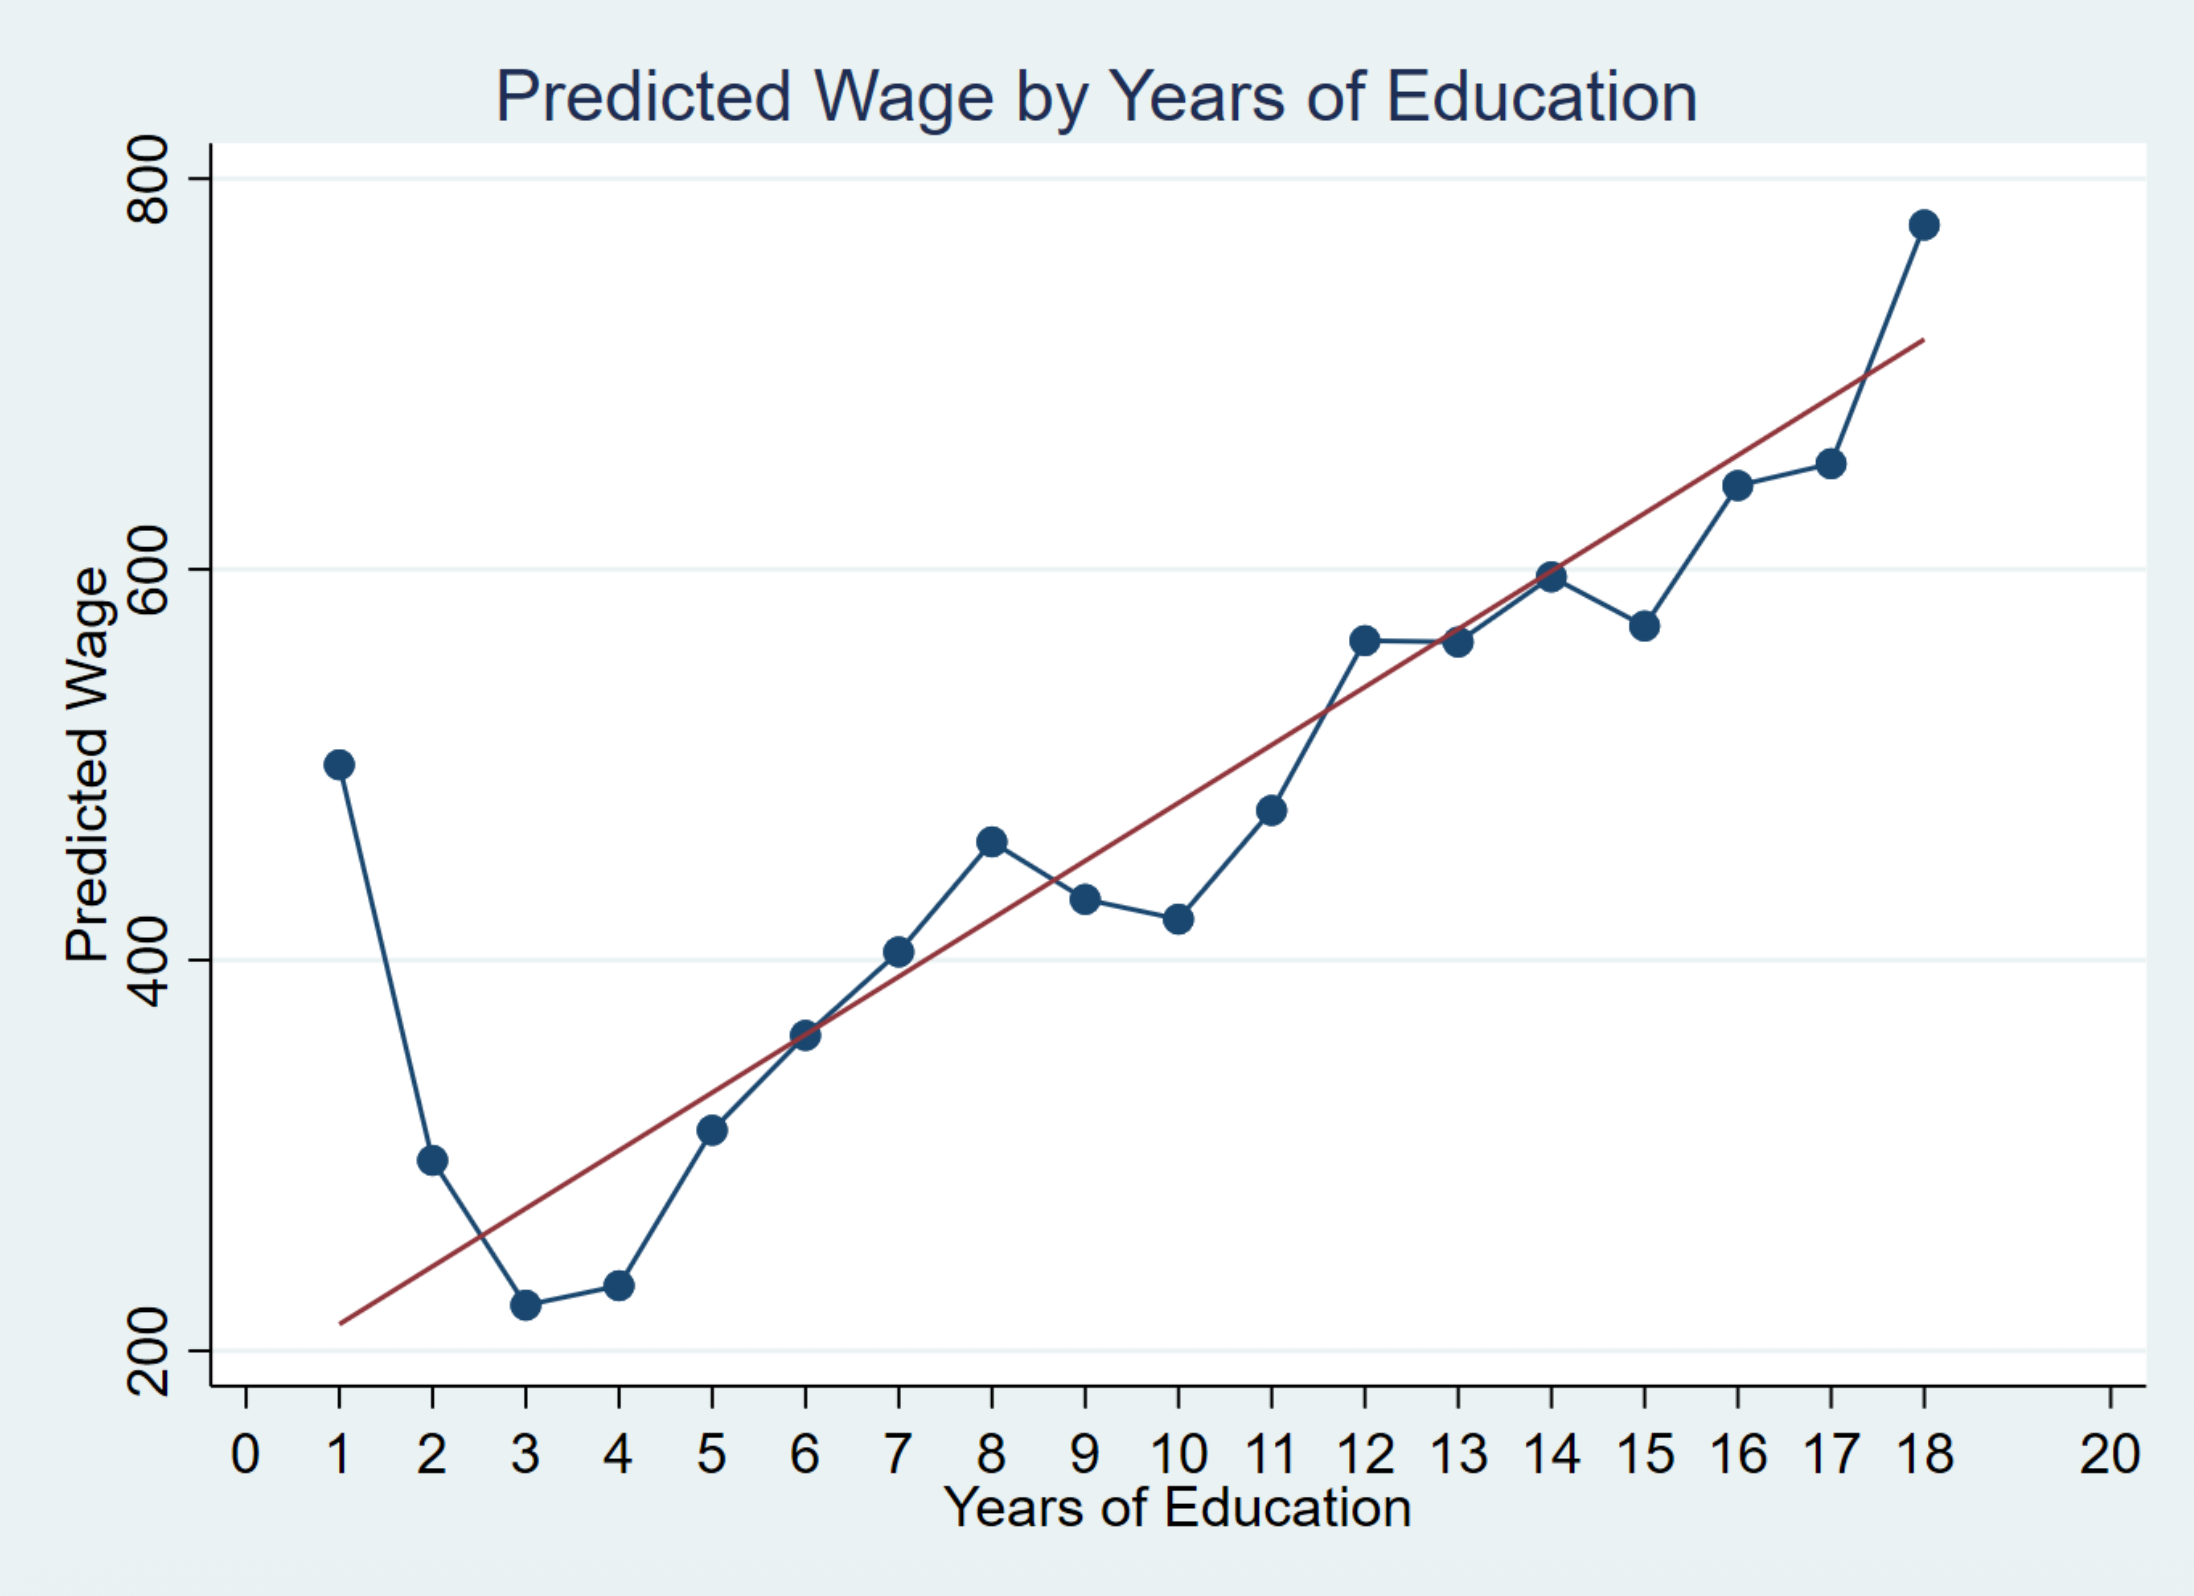
\includegraphics[width=0.78\textwidth]{images/1-22-1}
\end{figure}

There is a small sample problem for years of education less than 8. We trade off variance at this low end, getting a higher bias.

\begin{definition}[Best Linear Predictor]
	The best linear predictor of $y$ given $x$ is defined by
	\[
		\beta=\E\left[xx'\right]^{-1}\E\left[xy\right],
	\]
	where the FOC implies $\E\left[xy\right]=\E\left[xx'\right]\beta$. In order for these equations to have a unique solution, $\E\left[xx'\right]$ must be full rank/invertible. This is equivalent to there being no perfect multicollinearity in $x$; i.e., there is no $a\in \R^k\setminus \{0\}$ such that $x'a = 0$ with probability $1$.
\end{definition}

\section{OLS Estimation}

\begin{remark}	Given a sample $\{y_i,x_i\}_{i=1}^n$, we can apply the sample analogue principle\footnote{Now, $\theta(f)$ is defined as an $\argmin$ of an objective function. We find $\theta(\hat{f})$ now.} and solve the analogous in-sample problem:
	\[
		\min_{b\in\R^k}\frac{1}{n}\sum_{i=1}^n\left(y_i-x_i'b\right)^2
	\]
	to yield an estimator of $\beta$.\boxednote{The solution is $\hat{\beta} = (\frac{1}{n} \sum_i X_iX_i')^{-1} \frac{1}{n} \sum_i X_i Y_i$.} The first order conditions with respect to each $b_j$ imply that at the solution\boxednote{We think of a matrix of $x$ with the rows as observations $1:n$ and the columns as dimensions of $x$ from $1:k$. The first column will be $\vec 1$. Basically, we attach a $1$ to the meaningful characteristics of $x_i$ to get the intercept $\beta_0$ when multiplying by $X$. For example, if we want to consider predicting house price with number of bedrooms, a house would be represented by $(x_i;ly_i) = (1, \text{rooms}; \text{price})$. We want to allow the prediction line to not pass through the origin so the $\beta$s are interpretable as partial covariances.}:
	\[
		-2\cdot\frac{1}{n}\sum_{i=1}^n x_{ij}\left(y_i-x_i'\hat\beta\right)=0\quad\text{for all }1\le j\le k.
	\]

	Stacking these first order conditions gives
	\[
		\begin{pmatrix}
			\frac{1}{n}\sum_{i=1}^n x_{i1}(y_i-x_i'\hat\beta) \\
			\vdots                                            \\
			\frac{1}{n}\sum_{i=1}^n x_{ik}(y_i-x_i'\hat\beta)
		\end{pmatrix}
		=
		\frac{1}{n}\sum_{i=1}^n x_i(y_i-x_i'\hat\beta)=0.
	\]

	Adding $\left( \frac{1}{n} \sum_i x_i x_i' \right)\hat{\beta}$, we get that the FOCs imply
	\[
		\frac{1}{n}\sum_{i=1}^n x_iy_i=\left(\frac{1}{n}\sum_{i=1}^n x_ix_i'\right)\hat\beta.
	\]
	Provided $\frac{1}{n}\sum_{i=1}^n x_ix_i'$ is invertible, which occurs iff none of the columns $x_{\cdot j}$ are collinear, we obtain\boxednote{We can think of $(X_i,Y_i) \in \R^{k+1}$ so our estimator is an object in $\R^{k}$.}
	\[
		\hat\beta=\left(\frac{1}{n}\sum_{i=1}^n x_ix_i'\right)^{-1}\frac{1}{n}\sum_{i=1}^n x_iy_i.
	\]
\end{remark}

\begin{definition}[Fitted Values and Residuals]
	The $i$-th fitted value is:
	\[
		\hat y_i=x_i'\hat\beta.
	\]
	The $i$-th residual is
	\[
		\hat u_i=y_i-\hat y_i.
	\]
\end{definition}

\begin{remark}[FOC of OLS]
	The first order condition of the least squares minimization problem implies
	\[
		\sum_{i=1}^n x_i(y_i-x_i'\hat\beta)=\sum_{i=1}^n x_i\hat u_i=0.
	\]
	We can write this compactly as $X'\hat{u} = 0$.
\end{remark}

\begin{example}[Simple Linear Regression]
	Consider the simple linear model:
	\[
		y=\beta_0+\beta_1x_1+u,
	\]
	where now $x=(1,x_1)'$, and $\beta=(\beta_0,\beta_1)'$. Our earlier work implies\boxednote{Note that this expression for $\beta$ holds regardless of the dimension of $X$.}
	\[
		\beta=\E\left[xx'\right]^{-1}\E\left[xy\right].
	\]
	We have
	\begin{align*}
		\E\left[xx'\right]^{-1}
		&=\begin{pmatrix}
			1   & x_1   \\
			x_1 & x_1^2
		\end{pmatrix}^{-1}
		=\frac{1}{\E\left[x_1^2\right]-\E\left[x_1\right]^2}\begin{pmatrix}
			\E\left[x_1^2\right] & -x_1 \\
			-x_1                 & 1
		\end{pmatrix}, \\
		\E\left[xy\right]
		&=\begin{pmatrix}
			\E\left[y\right] \\
			\E\left[x_1y\right]
		\end{pmatrix}.
	\end{align*}
	It follows that\boxednote{\texthl{apparently this was done in the hw??}}
	\[
		\beta=\frac{1}{\operatorname{Var}(x_1)}\cdot\begin{pmatrix}
			\E\left[x_1^2\right] & -\E\left[x_1\right] \\
			-\E\left[x_1\right]  & 1
		\end{pmatrix}\begin{pmatrix}
			\E\left[y\right] \\
			\E\left[x_1y\right]
		\end{pmatrix}
		=\begin{pmatrix}
			\E\left[y\right]-\beta_1\E\left[x_1\right] \\
			\frac{\operatorname{Cov}(y,x_1)}{\operatorname{Var}(x_1)}
		\end{pmatrix}.
	\]
\end{example}

\begin{remark}[Slope Parameter and Correlation]
	Notice that
	\[
		\beta_1=\frac{\operatorname{Cov}(W,S)}{\operatorname{Var}(S)}=\sqrt{\frac{\operatorname{Var}(W)}{\operatorname{Var}(S)}}\cdot\operatorname{Corr}(W,S),
	\]
	so the slope coefficient is proportional to the correlation between wages and education (likely $>0$).

	Notice that increasing $\operatorname{Var}(W)$ stretches the scatter plot vertically (but leaves the correlation unchanged). The slope coefficient should increase in magnitude.

	Increasing $\operatorname{Var}(S)$ stretches the scatter plot horizontally (but leaves the correlation unchanged). The slope coefficient should decrease in magnitude.
\end{remark}

\begin{example}[Changing units of measurement]
	Suppose wages are now measured in cents per hour rather than dollars per hour. Let $\tilde W$ denote wages in cents:
	\[
		\tilde W=100W.
	\]
	Find the best linear predictor of $\tilde W$ given $S$, i.e. find $(\alpha_0,\alpha_1)$ such that\boxednote{\texthl{ why is including the condition on the expectation of $SU$, $U$ and finding the best linear predictor equivalent to the minimization problem without the error term?}}
	\[
		\tilde W=\alpha_0+\alpha_1S+U;\qquad \E\left[SU\right]=\E\left[U\right]=0.
	\]
	Find that
	\[
		\alpha_1=\frac{\operatorname{Cov}(\tilde W,S)}{\operatorname{Var}(S)}=\frac{100\operatorname{Cov}(W,S)}{\operatorname{Var}(S)}=100\beta_1,
	\]
	\[
		\alpha_0=\E\left[\tilde W\right]-\alpha_1\E\left[S\right]=100(\E\left[W\right]-\beta_1\E\left[S\right])=100\beta_0.
	\]
\end{example}

\begin{example}[Simple Linear Regression Estimation]
	Write the model for each individual $i=1,\ldots,n$ in the sample:
	\[
		y_i=\beta_0+\beta_1x_{i1}+u_i,
	\]
	and estimate the parameters using ordinary least squares:
	\[
		\hat\beta=\left(\frac{1}{n}\sum_{i=1}^n x_ix_i'\right)^{-1}\frac{1}{n}\sum_{i=1}^n x_iy_i
		=\begin{pmatrix}
			\bar y_n-\hat\beta_1\bar x_{1,n} \\
			\frac{\frac{1}{n}\sum_{i=1}^n x_{i1}y_i-\bar x_{1,n}\cdot\bar y_n}{\frac{1}{n}\sum_{i=1}^n x_{i1}^2-(\bar x_{1,n})^2}
		\end{pmatrix}.
	\]
\end{example}

\section{Matrix Notation and Projection}

\begin{remark}[Matrix Notation]
	First write the model for each observation $i=1,\ldots,n$:
	\[
		y_i=x_i'\beta+u_i.
	\]
	Stack the observations into matrices:
	\[
		\begin{pmatrix}
			y_1    \\
			y_2    \\
			\vdots \\
			y_n
		\end{pmatrix}
		=
		\underbrace{\begin{pmatrix}
			-x_1'- \\
			-x_2'- \\
			\vdots \\
			-x_n'-
		\end{pmatrix}}_{\text{design matrix}}
		\beta
		+
		\begin{pmatrix}
			u_1    \\
			u_2    \\
			\vdots \\
			u_n
		\end{pmatrix}.
	\]
	Therefore
	\[
		Y=X\beta+U,
	\]
	where the matrix $X$ is called the design matrix, with columns $X_1,\ldots,X_k\in\R^n$. If we have an intercept, then the first feature $X_1$ is a column of $1$s.

	The least squares minimization problem is
	\[
		\min_{b\in\R^k}\sum_{i=1}^n(y_i-x_i'b)^2\equiv\min_{b\in\R^k}(Y-Xb)'(Y-Xb) = \min_{B \in \R^k} \|Y - Xb\|^2
	\]
	because the sum of squares is just the inner product of $Y-Xb$ with itself.
	To see this, write \[
		\R^n \ni Y - Xb = \begin{bmatrix}
		y_1-x_1'b \\
		\vdots \\
		y_n - x_n'b
		\end{bmatrix} 
	,\] so \[
	\left( Y-Xb \right)'(Y-Xb) = \sum\limits_{i=1}^{n} \left( y_i - x_i'b \right)^2
	.\] Hence, we want to pick $b$ to minimize the distance from $Xb \in \operatorname{Span}(X)$ to $Y\in \R^n$ in the Euclidean norm. This is the point that is the orthogonal projection of $Y$ onto $\operatorname{Span}(X)$.

	We can expand the objective function as
	\[
		(Y-Xb)'(Y-Xb)=Y'Y-Y'Xb-b'X'Y+b'X'Xb=Y'Y-2Y'Xb+b'X'Xb,
	\]
	so the first order condition with respect to $b_j$ is
	\[
		-2\sum_{i=1}^n y_i\cdot x_{ij}+2\sum_{i=1}^n x_{ij}\cdot x_i'\hat\beta=0.
	\]
	Stack the first order conditions into a $k\times 1$ vector:
	\[
		-2\sum_{i=1}^n y_i\cdot x_i+2\left[\sum_{i=1}^n x_ix_i'\right]\hat\beta=0;\quad\text{or}\quad
		-2X'Y+2X'X\hat\beta=0.
	\]
	This yields $X'\left( Y- X\hat{\beta} \right) = 0$,\footnote{This says that every column of $X$ (row of $X'$) is orthogonal to the residual (row).} which is equivalent to (provided $X$ is full column rank):
	\[
		\hat\beta=(X'X)^{-1}X'Y.
	\]
\end{remark}

\begin{remark}	We have used the fact that
	\[
		\sum_{i=1}^n x_ix_i'=X'X,\qquad
		\sum_{i=1}^n y_ix_i=X'Y.
	\]
	To see why these identities hold, consider $X \in \R^{n\times k}$ and $X' \in \R^{k\times n}$, so \[
		X'X = \begin{bmatrix}
			\sum\limits_{i=1}^{n} x_{i_1}^2 & \sum\limits_{i=1}^{n} x_{i 1} x_{i 2} & \cdots \\
		\sum\limits_{i=1}^{n} x_{i 2}x_{i 1} & \sum\limits_{i=1}^{n} x_{i 2}^2 & \cdots \\
		\vdots & & \ddots
		\end{bmatrix} = \sum\limits_{i=1}^{n} X_i X_i'
	.\] Switching a transpose between matrices and vectors moves the transpose.

	The vector of fitted values is $\hat Y=X\hat\beta$, and the vector of residuals is $\hat U=Y-\hat Y$. The FOC of the least squares problem is equivalently written as $X'\hat U=0$. These are the normal equations.
\end{remark}

\begin{proposition}	$(X'X)^{-1}$ exists iff $X$ is full column rank.

	If $X$ is not full column rank, there exists $c\neq 0$ such that $Xc=0$, so $X'Xc=0$, implying $X'X$ is not invertible.

	If $X'X$ is not invertible, there exists $a\neq 0$ such that $X'Xa=0$, so $a'X'Xa=0$. But
	\[
		a'X'Xa=[Xa]'(Xa),
	\]
	which is a sum of squares which equals zero iff $Xa=0$. Since $a\neq 0$, $X$ is not full rank.

	In a simple linear regression, need there to be some variation in $\left( X_i \right)_{1:n}$ so it isn't collinear with the constant. Equivalently, need $\det(X'X)=(n-1)\cdot\widehat{\operatorname{Var}}(x)\neq 0$. When $X_i \in R^2$ with a column of $1$s, then we require that the 2nd column of $X$ is not identically some constant.
\end{proposition}

\begin{theorem}[Projection Theorem]
	Let $y\in\R^n$ and let $S$ be any nonempty subspace of $\R^n$ equipped with the dot product. There exists a unique point $\hat y$ such that $\|y-\hat y\|$ is minimized over $S$.\boxednote{Here, we are thinking of $S$ as a $k$-dimensional subspace of $\R^n$ --- the subset of $\R^n$ spanned by the columns of $X$.} A necessary and sufficient condition for $\hat y$ is that $\hat{y} \in S$ and $\hat y-y$ is orthogonal to every vector in $S$.

	By definition of $\hat\beta$, the vector $X\hat\beta$ is the closest (in the Euclidean norm) to $Y$ in the set of all vectors
	\[
		\{Xb:b\in\R^k\}=S(X),
	\]
	where $S(X)$ denotes the span of the columns of $X$. Given a vector $Y\in\R^n$ and a matrix $X\in\R^{n\times k}$, the projection of $Y$ onto $S(X)$ is the vector\footnote{We previously found $v^* = X\hat{\beta}$.}
	\[
		v^*\in\argmin_{v\in S(X)}\|Y-v\|^2.	
	\]

	While the coefficients $\hat{\beta}$ may not be unique (if $X$ is not full column rank), this theorem guarantees that $X\hat{\beta}$ is unique. 
\end{theorem}

\begin{example}	We can draw the following to provide intuition. Consider $n=2$, $k=2$, and a model with no intercept, so $y_i = \beta x_i + u_i$. Suppose $X = \begin{pmatrix}
	x_1 \\
	x_2
	\end{pmatrix} = \begin{pmatrix}
	1 \\
	0
	\end{pmatrix} $ and $Y = \begin{pmatrix}
	3 \\
	3
	\end{pmatrix} $.

	In this case, $S(X) = \{c \begin{pmatrix}
	1 \\
	0
	\end{pmatrix} : c\in \R\}$, so \[\hat{Y} = P_X Y = \begin{pmatrix}
	3 \\
	0
	\end{pmatrix}, \quad\hat{U} = \begin{pmatrix}
	0 \\
	3
\end{pmatrix}.\]

	We note that $P_X Y$ is the closest point to $Y$ in $S(X)$, while $\hat{U}$ is orthogonal to $S(X)$.
\end{example}


\begin{remark}	Restricting the minimizer to vectors in $S(X)$, the necessary and sufficient condition for the minimizer is
	\[
		x'(Y-\hat Y)=0
	\]
	for all $x\in S(X)$. Since the columns of $X$ are a basis of $S(X)$, this condition is equivalent to
	\[
		X'(Y-\hat Y)=0.
	\]
	$\hat Y\in S(X)$ means $\hat Y=Xb$ for some $b\in\R^k$. Thus
	\[
		X'Y=X'Xb\implies b=(X'X)^{-1}X'Y\implies\hat Y=X(X'X)^{-1}X'Y.
	\]
	That is, the projection of $Y$ onto $S(X)$ is given by $\hat Y=P_XY$, where $P_X$ is the projection matrix defined below.
\end{remark}

\begin{definition}[Projection Matrix]
	Since $X\hat\beta=X(X'X)^{-1}X'Y$, we call $P_X=X(X'X)^{-1}X'$ the projection matrix (it projects $Y$).

	The projection matrix is symmetric:
	\[
		P_X'=[X(X'X)^{-1}X']'=X[(X'X)^{-1}]'=X[(X'X)']^{-1}X'=P_X.
	\]
\end{definition}

\begin{remark}	$P_X$ is also idempotent (meaning $P_X\cdot P_X=P_X$), since:
	\[
		P_XP_X=X(X'X)^{-1}X'X(X'X)^{-1}X'=X(X'X)^{-1}X'=P_X,
	\]
	which reflects the fact that after a vector has been projected on to the span of the columns of $X$, it does not change as a result of the second projection. This is because the projected vector is already a linear combination of the columns of $X$.
\end{remark}

\begin{definition}[Residual Maker Matrix]
	The residual of the projection of $Y$ onto the columns of $X$ is
	\[
		Y-\hat Y=Y-P_XY=(I_n-X(X'X)^{-1}X')Y.
	\]
	Therefore, the matrix $M_X:=I_n-X(X'X)^{-1}X' = I_n - P_X$ is called the residual maker.

	$M_XY$ is the residual of the projection of $Y$ onto the space spanned by the columns of $X$.
\end{definition}

\begin{proposition}[Properties of Residual Maker]
	$M_X$ projects a vector onto the $n-k$ dimensional vector space orthogonal to the column space of $X$. This is called the orthogonal complement of $S(X)$.

	The residual of the projection $M_X y$ is $y - M_X y = P_X y \in S(X) \perp OC(S(X))$.

	Some properties:
	\begin{itemize}
		\item $P_XM_X=M_XP_X=0$, since $P_X(I-P_X)=P_X-P_XP_X=0$.
		\item $P_XX=X(X'X)^{-1}X'X=X$: Projecting $X$ onto its own span does nothing.
		\item $M_XX=X-P_XX=0$: Residual of projecting $X$ onto its own span is $0$.
		\item For any vector $y$, $y=P_Xy+M_Xy=\hat y+\hat u$.
	\end{itemize}
\end{proposition}

\section{$R^2$ and Goodness of Fit}

\begin{definition}[$R^2$]
	\begin{itemize}
		\item $\sum_{i=1}^n(y_i-\bar y)^2:=\text{TSS}$ is called the total sum of squares.
		\item $\sum_{i=1}^n(y_i-x_i'\hat\beta)^2:=\text{SSR}$ is the sum of squared residuals.
		\item $\sum_{i=1}^n(\hat y_i-\bar y)^2:=\text{ESS}$ is the explained sum of squares.
	\end{itemize}
	The coefficient of determination ($R^2$) is given by
	\[
		R^2=\frac{\text{ESS}}{\text{TSS}}.
	\]
\end{definition}

\begin{remark}	Immediately, we see that $SSR \le TSS$ because the $SSR$ is the residuals from letting our line of fit to have a free intercept and slope, while $TSS$ fixes a slope of $0$.
	$R^2$ measures how well OLS estimation of a linear model which includes a constant as a regressor fits a given dataset relative to a model only containing a constant. In other words, we are comparing two models:
	\begin{enumerate}[label=(\roman*)]
		\item $y = \beta_0 + u$, which implies $\hat{\beta}0^{OLS} = \overline{y}$
		\item $y = \beta_0 + \beta_1 x + \epsilon$,
	\end{enumerate}
	and seeing what fraction the SSR of the second model is of the SSR of the first model.
	

	We have:
	\[
		R^2=\frac{\text{ESS}}{\text{TSS}}=\frac{\sum_{i=1}^n(\hat y_i-\bar y_n)^2}{\sum_{i=1}^n(y_i-\bar y_n)^2}=1-\frac{\sum_{i=1}^n(y_i-x_i'\hat\beta)^2}{\sum_{i=1}^n(y_i-\bar y_n)^2},
	\]
	where the third equality follows from $SSR + ESS = TSS$ (shown later).

	The second and third equalities imply $0\le R^2\le 1$.

	$R^2=1$ iff $\text{SSR}=0$, which means $\hat U=0$.

	$R^2=0$ iff $\text{SSR}=\text{TSS}$, which implies all $y_i$ are identical and $\hat\beta=(\bar y,0,\ldots,0)$ provided $X$ is full column rank. In this case the model fits the data no better than a constant would; knowing $x$ does not help us predict $y$.
\end{remark}

\begin{proof} (Decomposition of $R^2$)
	Let $P_c=\mathbf{1}(\mathbf{1}'\mathbf{1})^{-1}\mathbf{1}'=\frac{1}{n}\mathbf{1}\mathbf{1}'$ be the projection matrix onto the span of the column vector of ones in $\R^n$. Then $P_cY=\frac{1}{n}\mathbf{1}\mathbf{1}'Y=\bar y_n\mathbf{1}$, so:
	\begin{align*}
		\text{TSS}&=\|Y-P_cY\|^2=\|M_cY\|^2 \\
		\text{ESS}&=\|P_XY-P_cY\|^2=\|P_XY-P_XP_cY\|^2=\|P_XM_cY\|^2 \\
		\text{SSR}&=\|Y-P_XY\|^2=\|M_XY\|^2=\|M_XM_cY\|^2.
	\end{align*}\boxednote{We see that \begin{align*}
		M_X M_c Y &= M_X Y - M_X P_c Y \\
		           &= M_X Y,
	\end{align*}since $P_c Y\in S(X)$ means $M_X P_c Y=0$.}

	Finally, since $P_XM_cY \in S(X)$ and $M_XM_cY \in OC(S(X))$ are orthogonal:
	\[
		\|M_XM_cY\|^2+\|P_XM_cY\|^2=\|M_XM_cY+P_XM_cY\|^2=\|M_cY\|^2,
	\]
	so $\text{ESS}+\text{SSR}=\text{TSS}$. This shows that
	\[
		R^2=\frac{\text{ESS}}{\text{TSS}}=1-\frac{\text{SSR}}{\text{TSS}}.
	\]
\end{proof}

\begin{remark}	High $R^2$ does not mean the linear model is ``correct'' in the sense that it provides a causal explanation of the relationship between $x$ and $y$.

	On the other hand, low $R^2$ does not preclude a causal relationship between $x$ and $y$ in a linear model.

	$R^2$ is an estimator of the population $R^2$, defined by
	\[
		R^2_{\text{pop}}=1-\frac{\operatorname{Var}(u)}{\operatorname{Var}(y)},
	\]
	since $\text{SSR}/n$ is an estimate of $\operatorname{Var}(u)$ and $\text{TSS}/n$ is an estimate of $\operatorname{Var}(y)$.

	Decomposing variance in $y$ as
	\[
		\operatorname{Var}(y):=\E\left[\operatorname{Var}(y\mid x)\right]+\operatorname{Var}(\E\left[y\mid x\right]).
	,\]
	the first term represents the unexplained variation in $y$\footnote{Since $\operatorname{Var}\left(y \mid x\right) = \E\left[\left( y - \E\left[y\mid x\right]  \right)^2\right]$ is the square of expected residual against the best linear predictor.}, while the second term represents variation in $y$ that is explained by the model.
\end{remark}

\begin{remark}	Note that SSR always weakly decreases when a regressor is added to the model.

	Suppose we estimate the intercept and slope parameters in the following models by OLS:
	\[
		A:y_i=\alpha_0+\alpha_1x_{i1}+u_i;\qquad
		B:y_i=\beta_0+\beta_1x_{i1}+\beta_2x_{i2}+v_i.
	\]
	Let $\text{SSR}_A$ be the SSR resulting from OLS estimation of $A$, and $\text{SSR}_B$ be the SSR resulting from OLS estimation of $B$.

	We have
	\[
		\text{SSR}_A=\min_{a_0,a_1}\sum_{i=1}^n(y_i-a_0-a_1x_{i1})^2=\sum_{i=1}^n(y_i-\hat\alpha_0-\hat\alpha_1x_{i1})^2;
	\]
	\[
		\text{SSR}_B=\min_{b_0,b_1,b_2}\sum_{i=1}^n(y_i-b_0-b_1x_{i1}-b_2x_{i2})^2=\sum_{i=1}^n(y_i-\hat\beta_0-\hat\beta_1x_{i1}-\hat\beta_2x_{i2})^2.
	\]

	$\text{SSR}_B\le\text{SSR}_A$: after finding $(\hat\alpha_0,\hat\alpha_1)$, setting $(b_0,b_1,b_2)=(\hat\alpha_0,\hat\alpha_1,0)$ is always feasible. In general, the optimal $b_2\ne0$, so adding $x_2$ strictly reduces SSR.

	This also means $R^2$ increases when adding regressors, because
	\[
		R^2_A=1-\frac{\text{SSR}_A}{\text{TSS}}\le 1-\frac{\text{SSR}_B}{\text{TSS}}=R^2_B.
	\]
\end{remark}

\begin{definition}[Adjusted $R^2$]
	Adjusted $R^2$ penalizes additional regressors, and is defined by
	\[
		\bar R^2=1-\frac{n-1}{n-k-1}\frac{\text{SSR}}{\text{TSS}}=1-\frac{n-1}{n-k-1}(1-R^2)\le R^2
	,\]
	where $k$ is the number of regressors (excluding the intercept) and $n$ is the sample size.
\end{definition}

\section{Finite Sample Properties of OLS}

Economists don't care too much about $R^2$ because it's a measure of prediction accuracy, not causality.

\begin{remark}[Gauss Markov Assumptions]
	We will work with the following assumptions to provide an ideal setting for linear regression, then derive the expectation and variance of OLS estimators:
	\begin{itemize}
		\item MLR.1: The model under consideration is
		      \[y=\beta_0+\beta_1x_1+\cdots+\beta_kx_k+u\equiv x'\beta+u.\]
		      \boxednote{By itself, MLR.1 imposes no restriction on $x$ because we can put $u = y - x'\beta$ and always represent $y$ in this way.}
		\item MLR.2: We observe an iid sample of $\{y_i,x_i\}_{i=1}^n$.
		\item MLR.3: There is no perfect collinearity in the sample (so $\left( X'X \right)^{-1}$ exists with probability $1$ and a unique $\hat\beta$ exists).
		\item MLR.4: $\E\left[u\mid x\right]=0$.\footnote{Hence, $\E\left[y \mid x\right] $ is a linear function of $x$.}
		\item MLR.5: (Homoskedasticity) $\operatorname{Var}(y\mid x)=\sigma^2$.\footnote{There is generally no good reason to believe in homoskedasticity. Correcting for heteroskedasticity would weight sample points where the error variance is lower, since these points give more information on the relationship between $y$ and $x$. This leads to generalized OLS, which is not used often because a heteroskedasticity correction is difficult (the standard deviation of the error as a function of $x$ is not known).}
	\end{itemize}
	MLR stands for multiple linear regression.
\end{remark}

\begin{proposition}	Suppose MLR.1--MLR.4 hold. By $\E\left[u\mid x\right] =0$ and since $(u_i,x_i)$ is independent of $x_j$ for $j\neq i$, we obtain for each $i$:
	\[
		0=\E\left[u_i\mid x_i\right]=\E\left[u_i\mid x_1,\ldots,x_n\right].
	\]
	This is equivalently written as
	\[
		\E\left[U\mid X\right]=0.
	\]
	This is in turn equivalent to
	\[
		\E\left[Y\mid X\right]=X\beta.
	\]
\end{proposition}
\begin{proof}
	(Bias.) It follows that
	\begin{align*}
		\E\left[\hat\beta\mid X\right]
		&=\E\left[(X'X)^{-1}X'Y\mid X\right]=(X'X)^{-1}X'\E\left[Y\mid X\right] \\
		&=(X'X)^{-1}X'X\beta=\beta.
	\end{align*}
	By the Law of Iterated Expectation:
	\[
		\E\left[\hat\beta\right]=\E\left[\E\left[\hat\beta\mid X\right]\right]=\beta,
	\]
	so $\hat\beta$ is unbiased.

	(Variance.) Suppose in addition that $\operatorname{Var}(u_i\mid x_i)=\sigma^2$. (MLR.5)

	Since the error variance does not depend on the value of $x_i$, it is called homoskedastic. If the error variance depends on $x_i$, $u_i$ is heteroskedastic and MLR.5 fails.

	Under homoskedasticity,
	\[
		\operatorname{Var}(U\mid X)=\sigma^2I_n.
	\]
	To see this, note that the $(i,j)$ entry is given by
	\[
		\operatorname{Var}(U\mid X)_{i,j}=\E\left[UU'\mid X\right]_{i,j}=\E\left[u_iu_j\mid X\right]=
		\begin{cases}
			\E\left[u_i^2\mid x_i\right]      & i=j      \\
			\E\left[u_iu_j\mid x_i,x_j\right] & i\neq j.
		\end{cases}
	\]

	We have $\E\left[u_i^2\mid x_i\right]=\sigma^2$ because
	\[
		\E\left[u_i^2\mid x_i\right]-\underbrace{(\E\left[u_i\mid x_i\right])^2}_{=0}=\operatorname{Var}(u_i\mid x_i)=\sigma^2.
	\]
	We also have that for $i\ne j$,
	\[
		\E\left[u_iu_j\mid x_i,x_j\right]=\E\left[u_i\E\left[u_j\mid u_i,x_i,x_j\right]\mid x_i,x_j\right]=\E\left[u_i\E\left[u_j\mid x_j\right]\mid x_i,x_j\right]=0.
	\] The off diagonal elements are $0$ because of MLR.2,\footnote{MK: and because of MLR.4, I think.} \emph{not} because of MLR.5.

	Under heteroskedasticity, the off diagonal elements are still $0$ but\[\E[u_i^2\mid x_i]=f(x_i),\]so
	\[
		\operatorname{Var}(U\mid X)=
		\begin{pmatrix}
			f(x_1) & 0      & 0      & 0      \\
			0      & f(x_2) & 0      & 0      \\
			0      & 0      & \ddots & 0      \\
			0      & 0      & 0      & f(x_n)
		\end{pmatrix} =: \Omega
		.\]

	We now conclude that (*)
	\[
		\operatorname{Var}(\hat\beta\mid X)=\operatorname{Var}(\beta+(X'X)^{-1}X'U\mid X)=(X'X)^{-1}X'\Omega X(X'X)^{-1}.
	\]
	Under homoskedasticity, $\Omega=\sigma^2I_n$, and so the variance becomes
	\[
		\operatorname{Var}(\hat\beta\mid X)=\sigma^2(X'X)^{-1}X'I_nX(X'X)^{-1}=\sigma^2(X'X)^{-1}.
	\]

	(*) follows from $\hat{\beta} = \beta + \left( \underbrace{\left( X'X \right)^{-1}X'}_{A(X)} U \mid X \right)$, so \[
		\operatorname{Var}\left(\left( \hat{\beta} \mid X \right)\right)= A(X) \operatorname{Var}\left(U \mid X\right) A(X)' = \sigma^2 \left( X'X \right)^{-1}
	,\] where the last equality follows from MLR.5.
\end{proof}

\begin{theorem}[Gauss-Markov Theorem]
	Under MLR.1--5, the OLS estimator is the ``best linear unbiased estimator'', which means it has the ``smallest'' variance in the class of linear estimators that are also unbiased conditional on $X$. This result is known as the Gauss-Markov Theorem.

	Our goal is to show that
	\[
		\operatorname{Var}(\hat\beta\mid X)=\sigma^2(X'X)^{-1}
	\]
	is ``smaller'' than the conditional variance of any other estimator $\tilde\beta=A(X)Y$ which also satisfies $\E\left[\tilde\beta\mid X\right]=\beta$. Precisely: $\operatorname{Var}(\tilde\beta\mid X)-\operatorname{Var}(\hat\beta\mid X)=D$ is a positive-semidefinite matrix.
\end{theorem}

\begin{remark}	In particular, let $r$ be a $k\times 1$ vector, and let $r'\beta$ denote a linear combination of the $\beta_j$. The Gauss-Markov theorem implies that $r'\hat\beta$ is the Best Linear Unbiased Estimator of $r'\beta$, since
	\[
		\operatorname{Var}(r'\tilde\beta\mid X)-\operatorname{Var}(r'\hat\beta\mid X)=r'\operatorname{Var}(\tilde\beta\mid X)r-r'\operatorname{Var}(\hat\beta\mid X)r=r'Dr\ge 0.
	\]
	For example, if $r=(0,0\ldots,0,\underbrace{1}_{\text{$j$-th position}},0,\ldots,0)$, then $r'\hat\beta=\hat\beta_j$, and so $\operatorname{Var}(\hat\beta_j\mid X)\le\operatorname{Var}(\tilde\beta_j\mid X)$.
\end{remark}

\begin{proof}(Gauss-Markov Theorem)
	Now consider any other linear unbiased (conditional on $X$) estimator of $\beta$ defined by \[
		\tilde{\beta} = A(X) Y
	.\] Recall that $\hat{\beta} = A(X) = \left( X'X \right)^{-1}X'$. Note that 
	\begin{align*}
		\E\left[\tilde{\beta} \mid X\right]  &= \E\left[A(X) Y \mid X\right]  \\
		&= A(X) \E\left[Y \mid X\right]  \\
		&= A(X) X \beta
	,\end{align*}
	which must be equal to $\beta$ for any $\beta \in \R^k$ if $\tilde{\beta}$ is unbiased. In this case, for any $\beta \in \R^k$, \[
		\left( A(X) X - I_k \right)\beta = 0
	,\] so \[
		A(X)X = I_k
	.\] 
	Therefore, if we require $\hat{\beta}$ to be unbiased, we require $A(X) X = I_k$. Note that $A(X)$ as defined in OLS satisfies this.

	From now on, write $A := A\left( X \right)$.

	Next, we compute the variance of $\tilde{\beta} = AY$ conditional on $X$:
	\[
		\operatorname{Var}\left(\tilde{\beta} \mid X\right) = \operatorname{Var}(AY\mid X)=A\operatorname{Var}(Y\mid X)A'=A\operatorname{Var}(U\mid X)A'=\sigma^2AA'.
	\]
	If $A=(X'X)^{-1}X'$, we obtain the OLS estimator, with variance $\sigma^2(X'X)^{-1}$.

	We really want to show that $\operatorname{Var}\left(\tilde{\beta}\mid X\right) \ge \operatorname{Var}\left(\hat{\beta} \mid X\right)$. But how should we define an ordering of matrices? One way is to say that the first matrix is larger if the difference of the first minus the second is positive semidefinite. This is because taking a linear combination of the $\hat{\beta}$ estimate's components with a vector $r$ multiplies the variance by $r$ and $r'$ on either side, respectively.

	Define $C = A - (X'X)^{-1}X'$, so that $A = C + (X'X)^{-1}X'$. Note that the unbiasedness constraint $AX = I_k$ gives
	\[
		CX = AX - (X'X)^{-1}X'X = I_k - I_k = 0.
	\]
	Expanding $AA'$:
	\begin{align*}
		AA' &= \Bigl(C + (X'X)^{-1}X'\Bigr)\Bigl(C + (X'X)^{-1}X'\Bigr)' \\
		    &= CC' + \underbrace{CX}_{=\,0}(X'X)^{-1} + (X'X)^{-1}\underbrace{(CX)'}_{=\,0} + (X'X)^{-1}X'X(X'X)^{-1} \\
		    &= CC' + (X'X)^{-1}.
	\end{align*}
	Therefore,
	\begin{align*}
		\operatorname{Var}\left(\tilde{\beta} \mid X\right) - \operatorname{Var}\left(\hat{\beta} \mid X\right)
			&= \sigma^2 AA' - \sigma^2(X'X)^{-1} \\
			&= \sigma^2\bigl[CC' + (X'X)^{-1}\bigr] - \sigma^2(X'X)^{-1} \\
			&= \sigma^2 CC'.
	\end{align*}
	Because $CC'$ is always positive semidefinite, we are done.

\end{proof}

\begin{remark}[Why positive semidefiniteness?]
	In particular,
	\begin{align*}
		\operatorname{Var}\left(\left( r' \hat{\beta} \mid X \right)\right) - \operatorname{Var}\left( r' \hat{\beta} \mid X\right) &=  r' \operatorname{Var}\left(\tilde{\beta} \mid X\right)r - r' \operatorname{Var}\left(\hat{\beta} \mid X\right)r \\
		&= r' \left[ \operatorname{Var}\left(\tilde{\beta }\mid X\right) - \operatorname{Var}\left(\hat{\beta} \mid X\right) \right]r \\
		&= \sigma^2 r' C C' r \ge 0
	,\end{align*}
	where the inequality follows from positive semidefiniteness of $C C'$. Therefore $r' \hat{\beta}$ is at least as efficient as $r' \tilde{\beta}$ for estimate $r' \beta$.
	In particular, \[
		\operatorname{Var}\left(\hat{\beta}_j \mid X\right) \le \operatorname{Var}\left( \left( \tilde{\beta}_j \mid X \right)\right)
	\] for any $j$. The OLS estimator $\hat{\beta}$ is efficient in the sense that componentwise, it achieves the lowest variance of an unbiased linear estimator of the conditional mean.\footnote{In fact, OLS is the best unbiased estimator (not restricting to just linear estimators). But doubly in fact, the only unbiased estimators are linear.}
\end{remark}


% Week 4 Slides
\section{Large Sample Properties of OLS}

\begin{assumption}	Now drop the assumptions that $\E\left[u_i \mid x_i\right] = 0$\footnote{i.e. that the relationship between $y$ and $x$ is linear.} and $\operatorname{Var}(u_i \mid x_i) = \sigma^2$ but assume we have an iid sample $\{y_i, x_i\}_{i=1}^n$.
	
	The model is \[
		y = x'\beta + u
	.\] 
	
	Suppose that $\E\left[ux\right] = 0$ and that $\E\left[xx'\right] $ is invertible. Note that $\frac{1}{n} \sum_{i=1}^{n} x_i x_i'$ may not be invertible under these assumptions (which was MLR.3), but it is invertible with probability approaching one because $\E\left[xx'\right] ^{-1}$ exists.
	
	In other words, the population condition that $\E\left[x x'\right]^{-1}$ existing is stronger (as in implies the sample condition) than the sample condition of $\frac{1}{n}\sum_{i=1}^{n} x_i x_i'$ being invertible.\boxednote{This is because if $\E\left[x x'\right] ^{-1}$ exists, the determinant of $\E\left[x x'\right] $ as a continuous function of $x$ is nonzero; convergence in probability gives a neighborhood of invertible matrices for which the determinant is nonzero. By the WLLN/convergence in probability, $\frac{1}{n}\sum x_i x_i'$ is eventually within this ball a.s.}
\end{assumption}

\begin{proposition}[Consistency]
	Under these weaker assumptions, the OLS estimator is consistent.
\end{proposition}
\begin{proof}
	First, note that \[
		\frac{1}{n} \sum_{i=1}^{n} x_i x_i' \xrightarrow{p} \E\left[xx'\right] ; \quad \frac{1}{n} \sum_{i=1}^{n} x_i y_i \xrightarrow{p} \E\left[xy\right] 
	.\] 
	by the law of large numbers, because $\{x_i x_i'\}_{i \ge 1}$ is an iid sequence of random matrices with expectation $\E\left[xx'\right] $, and $\{x_i y_i\}_{i \ge 1}$ is an iid sequence of random vectors with expectation $\E\left[xy\right] $.

	Marginal convergence in probability implies joint convergence in probability: \[
		\left( \frac{1}{n} \sum_{i=1}^{n} x_i x_i', \frac{1}{n} \sum_{i=1}^{n} x_i y_i \right) \xrightarrow{p} \left( \E\left[xx'\right] , \E\left[xy\right]  \right) 
	.\] 
	
	Now let $g(x,y) = x^{-1}y$, where $x^{-1}$ denotes a matrix inverse. $g$ is continuous if $x$ is invertible (matrix version of $x \ne 0$).
	
	It therefore follows by the continuous mapping theorem that \[
		\left( \frac{1}{n} \sum_{i=1}^{n} x_i x_i' \right)^{-1} \frac{1}{n} \sum_{i=1}^{n} x_i y_i \xrightarrow{p} \E\left[xx'\right] ^{-1} \E\left[xy\right] = \beta + \E\left[xx'\right] ^{-1} \E\left[xu\right] = \beta
	\] by plugging in $y = x' \beta + u$. 
\end{proof}

\begin{proposition}[Asymptotic Normality of OLS]
	Assume $\operatorname{Var}(xu)$ exists also. Then because $\E\left[xu\right] = 0 \implies \left( \E\left[xu\right]  \right)^2 = 0$, \[
		\operatorname{Var}(xu) = \E\left[xu(xu)'\right] = \E\left[u^2 xx'\right] 
	.\] 
	
	We have \[
		\sqrt{n} \left( \hat{\beta}_n - \beta \right) \xrightarrow{d} N(0, \Sigma)
	,\] where $\Sigma = \E\left[xx'\right] ^{-1} \operatorname{Var}(xu) \E\left[xx'\right] ^{-1}$.
\end{proposition}

\begin{proof}
	First note that \[
		\sqrt{n} \left( \hat{\beta}_n - \beta \right) = \left( \frac{1}{n} \sum_{i=1}^{n} x_i x_i' \right)^{-1} \frac{1}{\sqrt{n}} \sum_{i=1}^{n} x_i u_i
	.\] 

	Since the sequence of vectors $\left\{ (y_i, x_i')' \right\}_{i \ge 1}$ is iid, the sequence $\{x_i (y_i - x_i' \beta)\}_{i \ge 1}$ is iid. Therefore, the CLT implies:\boxednote{CLT applies:\begin{align*}\tfrac{1}{\sqrt{n}}\sum_i (X_i-\mu)&=\sqrt{n}(\bar X_n-\mu).\end{align*}} \[
		\frac{1}{\sqrt{n}} \sum_{i=1}^{n} x_i u_i \xrightarrow{d} N(0, \operatorname{Var}(xu))
	.\] 
	
	Applying Slutsky's Theorem gives \[
		\left( \frac{1}{n} \sum_{i=1}^{n} x_i x_i' \right)^{-1} \frac{1}{\sqrt{n}} \sum_{i=1}^{n} x_i u_i \xrightarrow{d} N(0, \Sigma)
	,\] as desired.
\end{proof}

\section{Estimation of $\Sigma$}

Deriving asymptotic normality of $\hat{\beta}$ will enable us to conduct hypothesis tests about the unknown parameter $\beta$.

Since we do not know $\Sigma$, we must construct a consistent estimator of it to yield an asymptotic distribution whose quantiles are known so we may conduct tests.

For the time being (the next two propositions), suppose MLR.4 and MLR.5 hold, so we have an easy case in which $\E\left[u \mid x\right] = 0$ and $\operatorname{Var}(u \mid x) = \sigma^2$. Then \[
	\operatorname{Var}(xu) = \E\left[u^2 xx'\right] = \E\left[\E\left[u^2 \mid x\right] xx'\right] = \E\left[\operatorname{Var}\left(u \mid x\right) x x'\right] = \sigma^2 \E\left[xx'\right] 
.\] 

It follows that \[
	\Sigma =  \E\left[x x'\right] ^{-1} \sigma^2  \E\left[x x'\right]  \E\left[x x'\right] ^{-1} = \sigma^2 \E\left[xx'\right] ^{-1}
.\] 


\begin{proposition}[$\hat{\sigma}^2$ is consistent]
	A natural estimator of $\E\left[xx'\right] ^{-1}$ is $\left( \frac{1}{n} \sum_{i=1}^{n} x_i x_i' \right)^{-1}$.\boxednote{The degree of freedom correction $k$ is the number of $\beta_j$s we are estimating. It is the width of the design matrix. Note that the adjusted $R^2$ does not count the intercept in its $k$, but when $k$ is the df correction, it is just always the number of $\beta$s to be estimated.}
	
	It remains to find a consistent estimator of $\sigma^2$. We use \[
		\hat{\sigma}^2 = \frac{1}{n-k} \sum_{i=1}^{n} \hat{u}_i^2 = \frac{\text{SSR}}{n-k}
	.\] 
	
	Next, note that $\hat{U} = M_X Y = M_X (X\beta + U) = M_X U$, so\footnote{The third equality follows from symmetry and idempotency of $M_X$.} \[
		\text{SSR} = \|M_X U\|^2 = U' M_X' M_X U = U' M_X U = U'U - U' P_X U
	.\] 
	Therefore, \[
		\begin{aligned}
			\hat{\sigma}^2
			&= \frac{\operatorname{SSR}}{n-k}
			= \frac{\operatorname{SSR}}{n}\frac{n}{n-k} \\
			&= \frac{n}{n-k} \left( \frac{1}{n} \sum_{i=1}^{n} u_i^2 - \left( \frac{1}{n} \sum_{i=1}^{n} u_i x_i' \right) \left( \frac{1}{n} \sum_{i=1}^{n} x_i x_i' \right)^{-1} \left( \frac{1}{n} \sum_{i=1}^{n} x_i u_i \right) \right) \\
			&\xrightarrow{p} \sigma^2 - 0 \cdot \E\left[xx'\right]^{-1} \cdot 0
			= \sigma^2
		\end{aligned}
	,\] by the continuous mapping theorem.
	
	Another application of the continuous mapping theorem implies that a consistent estimator of $\Sigma$ is given by \[
		\hat{\Sigma} = \hat{\sigma}^2 \left( \frac{1}{n} \sum_{i=1}^{n} x_i x_i' \right)^{-1} \xrightarrow{p} \sigma^2 \E\left[x x'\right]^{-1} = \Sigma
	.\] 
\end{proposition}

\begin{proposition}[$\hat{\sigma}^2$ is unbiased]
	We now show the degrees of freedom correction $n-k$ yields an unbiased estimate of $\sigma^2$. To see this, note that \[
		(n-k) \hat{\sigma}^2 = \text{SSR}
	,\] and
	\[
		\begin{aligned}
			\E\left[\text{SSR} \mid X\right]
			&= \E\left[U'U \mid X\right] - \E\left[U' P_X U \mid X\right] \\
			&= \sum_{i=1}^{n} \E\left[u_i^2 \mid X\right] - \E\left[U' P_X U \mid X\right] \\
			&= n\sigma^2 - \E\left[U' P_X U \mid X\right]
		\end{aligned}
	.\]
	We want to remove $P_X$ from the expectation, but it is in the middle of the product.

	Since expectations can be exchanged with summations, for a random matrix $A$: \[
		\E\left[\operatorname{tr}(A)\right] = \operatorname{tr}(\E\left[A\right] )
	.\] 
	
	The trace has a special property called invariance under cyclic permutations.
	
	For our purposes, this means that for any matrices $A, B$ such that $AB$ and $BA$ are well defined: \[
		\operatorname{tr}(AB) = \operatorname{tr}(BA)
	.\] 
	Since $U' P_X U$ is a scalar, it equals its trace, so \begin{align*}
		\E\left[U' P_X U \mid X\right] &= \E\left[\operatorname{tr}(U' P_X U) \mid X\right] \\ &= \E\left[\operatorname{tr}(P_X U U') \mid X\right] \\
									   &= \operatorname{tr}\left( P_X \E\left[UU' \mid X\right]  \right) \\
									   &= \operatorname{tr}(P_X \sigma^2 I_n) \\ &= \sigma^2 \operatorname{tr}\left( X(X'X)^{-1}X' \right)  \\ &= \sigma^2 \operatorname{tr}\left( X'X (X'X)^{-1} \right) \\ &= \sigma^2 \operatorname{tr}(I_k) \\ &= k\sigma^2
	.\end{align*} 
	
	This implies $\E\left[\text{SSR} \mid X\right] = n\sigma^2 - k\sigma^2 = (n-k)\sigma^2$, so $ \hat{\sigma}^2 = \frac{\E\left[\operatorname{SSR}\mid X\right] }{n-k}$ is an unbiased estimator of $\sigma^2$.
\end{proposition}

\begin{remark}
	If we do not assume $\E\left[u \mid x\right] = 0$ and $\operatorname{Var}(u \mid x) = \sigma^2$, $\Sigma$ does not simplify, and we use \[
		\hat{\Sigma} = \left( \frac{1}{n} \sum_{i=1}^{n} x_i x_i' \right)^{-1} \left( \frac{1}{n} \sum_{i=1}^{n} \hat{u}_i^2 x_i x_i' \right) \left( \frac{1}{n} \sum_{i=1}^{n} x_i x_i' \right)^{-1}
	.\] 
	
	Note that this is identical to $n \cdot (X'X)^{-1} X' \hat{\Omega} X (X'X)^{-1}$, where \[
		\hat{\Omega} = 
		\begin{pmatrix}
			\hat{u}_1^2 & 0 & 0 & 0 \\
			0 & \hat{u}_2^2 & 0 & 0 \\
			0 & 0 & \ddots & 0 \\
			0 & 0 & 0 & \hat{u}_n^2
		\end{pmatrix}
	.\] 

	Proving consistency boils down to showing that \[
		\frac{1}{n} \sum_{i=1}^{n} \hat{u}_i^2 x_i x_i' \xrightarrow{p} \E\left[u^2 xx'\right] 
	.\] 
	
	First, decompose this quantity as \[
		\frac{1}{n} \sum_{i=1}^{n} \hat{u}_i^2 x_i x_i' = \frac{1}{n} \sum_{i=1}^{n} u_i^2 x_i x_i' + \frac{1}{n} \sum_{i=1}^{n} (\hat{u}_i^2 - u_i^2) x_i x_i'
	.\] 

	We have \[
		\frac{1}{n} \sum_{i=1}^{n} u_i^2 x_i x_i' \xrightarrow{p} \E\left[u^2 xx'\right] 
	,\] so it remains to show that \[
		\frac{1}{n} \sum_{i=1}^{n} (\hat{u}_i^2 - u_i^2) x_i x_i' = o_p(1)
	.\] 
	
	We prove that every element of this matrix converges to zero in probability.

	Fix $j,k$ element $\frac{1}{n} \sum_{i=1}^{n} (\hat{u}_i^2 - u_i^2) x_{i,j} x_{i,k}$, and observe that \[
		\begin{aligned}
			\left| \frac{1}{n} \sum_{i=1}^{n} (\hat{u}_i^2 - u_i^2) x_{i,j} x_{i,k} \right|
			&\le \frac{1}{n} \sum_{i=1}^{n} |\hat{u}_i^2 - u_i^2| |x_{i,j} x_{i,k}| \\
			&\le \max_{1 \le i \le n} |\hat{u}_i^2 - u_i^2| \frac{1}{n} \sum_{i=1}^{n} |x_{i,j} x_{i,k}|
		\end{aligned}
	.\] 
	
	Since \[
		\frac{1}{n} \sum_{i=1}^{n} |x_{i,j} x_{i,k}| \xrightarrow{p} \E\left[|x_{i,j} x_{i,k}|\right] 
	,\] it is sufficient to prove \[
		\max_{1 \le i \le n} |\hat{u}_i^2 - u_i^2| \xrightarrow{p} 0
	.\] 

	To this end, note that \[
		\hat{u}_i - u_i = x_i' (\beta - \hat{\beta}_n)
	,\] so since $\hat{u}_i = y_i - x_i' \hat{\beta}_n = x_i' (\beta - \hat{\beta}_n) + u_i$, we have: \[
		\begin{aligned}
			|\hat{u}_i^2 - u_i^2|
			&= |x_i' (\beta - \hat{\beta}_n) (\hat{u}_i + u_i)| \\
			&= |x_i' (\beta - \hat{\beta}_n) (x_i' (\beta - \hat{\beta}_n) + 2u_i)| \\
			&= \left| \left( x_i' (\beta - \hat{\beta}_n) \right)^2 + 2u_i x_i' (\beta - \hat{\beta}_n) \right| \\
			&\le \left| \left( x_i' (\beta - \hat{\beta}_n) \right)^2 \right| + 2 \left| u_i x_i' (\beta - \hat{\beta}_n) \right|
		\end{aligned}
	.\] 

	Next, using the Cauchy-Schwarz inequality, we obtain \[
		\begin{aligned}
			\max_{1 \le i \le n} |\hat{u}_i^2 - u_i^2|
			&\le \|\beta - \hat{\beta}_n\|^2 \max_{1 \le i \le n} \|x_i\|^2 + 2 \|\beta - \hat{\beta}_n\| \max_{1 \le i \le n} \|x_i u_i\| \\
			&= \left\| \sqrt{n} (\beta - \hat{\beta}_n) \right\|^2 \frac{\max_{1 \le i \le n} \|x_i\|^2}{n} \\
			&\quad + 2 \left\| \sqrt{n} (\beta - \hat{\beta}_n) \right\| \frac{\max_{1 \le i \le n} \|x_i u_i\|}{\sqrt{n}}
		\end{aligned}
	.\] 

	Since $\sqrt{n} (\beta - \hat{\beta}_n)$ converges in distribution, we must show: \[
		\frac{\max_{1 \le i \le n} \|x_i\|^2}{n} \xrightarrow{p} 0
		\qquad \text{and} \qquad
		\frac{\max_{1 \le i \le n} \|x_i u_i\|}{\sqrt{n}} \xrightarrow{p} 0
	.\] 
\end{remark}

\begin{lemma}	Let $\{Z_i\}_{i \ge 1}$ be a sequence of identically distributed random vectors such that $\E\left[\|Z_i\|^r\right] < \infty$. Then \[
		\frac{\max_{1 \le i \le n} \|Z_i\|}{n^{1/r}} \xrightarrow{p} 0
	.\] 
\end{lemma}

\begin{proof}
	Fix $\epsilon > 0$ and note that
	\begin{align*}
		\P\left( \max_{1 \le i \le n} \|Z_i\| > \epsilon n^{1/r} \right) &= \P\left( \cup_{i=1}^n \{\|Z_i\|^r > \epsilon^r n\} \right) \\
		&\le \sum_{i=1}^{n} \P\left( \|Z_i\|^r > \epsilon^r n \right) \\
		&= \sum_{i=1}^{n} \P\left( \|Z_i\|^r \mathds{1}(\|Z_i\|^r > \epsilon^r n) > \epsilon^r n \right) \\
		&\le \frac{1}{n\epsilon^r} \sum_{i=1}^{n} \E\left[\|Z_i\|^r \mathds{1}(\|Z_i\|^r > \epsilon^r n)\right] \\
		&= \frac{1}{\epsilon^r} \E\left[\|Z_i\|^r \mathds{1}(\|Z_i\|^r > \epsilon^r n)\right] \\
		&\to 0
	.\end{align*}
\end{proof}

\begin{remark}	The second equality holds because \[
		\{\|Z_i\|^r > \epsilon^r n\} = \{\|Z_i\|^r \mathds{1}(\|Z_i\|^r > \epsilon^r n) > \epsilon^r n\}
	.\] 
	
	The second inequality follows by Markov's inequality and the third equality because the $Z_i$ have identical distribution.
	
	Convergence to $0$ holds by an application of the dominated convergence theorem, since $\E\left[\|Z_i\|^r\right] < \infty$.
	
	Finally, since $\E\left[\|x\|^2\right] < \infty$ and $\E\left[\|ux\|^2\right] < \infty$, we conclude that \[
		\max_{1 \le i \le n} |\hat{u}_i^2 - u_i^2| \xrightarrow{p} 0
	,\] so \[
		\frac{1}{n} \sum_{i=1}^{n} (\hat{u}_i^2 - u_i^2) x_i x_i' \xrightarrow{p} 0
	.\] 
\end{remark}

\begin{remark}[Asymptotic vs. finite sample variance]
	Under assumptions MLR.1-5 (stronger than necessary for asymptotic results): \[
		\operatorname{Var}\left( \sqrt{n} (\hat{\beta} - \beta) \mid X \right) = \sigma^2 \left( \frac{1}{n} \sum_{i=1}^{n} x_i x_i' \right)^{-1}
	.\] 
	
	This quantity converges in probability to the variance of the asymptotic distribution: \[
		\operatorname{AVar}(\hat{\beta}) = \sigma^2 \E\left[x_i x_i'\right] ^{-1}
	.\] 
\end{remark}

\section{Partitioned Regression and Coefficient Interpretation}

Motivation (``partialling out'').
Consider a regression with a single regressor of interest and a set of controls,
\[
	y_i = \beta_1 x_{i1} + x_{i2}'\beta_2 + u_i,
\]
and suppose $x_{i1}$ can be decomposed into the part explained by $x_{i2}$ and an orthogonal residual,
\[
	x_{i1} = x_{i2}'\gamma + v_i, \qquad \E[x_{i2} v_i] = 0.
\]
If (as in the linear projection/OLS setup) we also have $\E[x_{i2}u_i]=0$, then only the variation in $x_{i1}$ that is orthogonal to the span of $x_{i2}$ can identify $\beta_1$.
This is the sense in which $\beta_1$ measures the effect of $x_{1}$ on $y$ ``holding $x_2$ fixed''.

\begin{proposition}[Frisch--Waugh--Lovell in sample form]
	Suppose the (sample) linear regression model is written as
	\[
		Y = X_1\beta_1 + X_2\beta_2 + U
	\]
	with $X=[X_1 \mid X_2]$ full column rank and let $\hat{\beta}=(\hat{\beta}_1',\hat{\beta}_2')'$ be the OLS estimator from regressing $Y$ on $X$.
	Then
	\[
		\hat{\beta}_1
		= (X_1' M_{X_2} X_1)^{-1} X_1' M_{X_2} Y
		= (X_1^{*'}X_1^*)^{-1} X_1^{*'} Y^*
	\]
	where $M_{X_2} := I_n - P_{X_2}$, $X_1^* := M_{X_2}X_1$ and $Y^* := M_{X_2}Y$.
	Moreover, because $X_1^{*'}P_{X_2} = 0$, we can equivalently replace $Y^*$ with $Y$:
	\[
		\hat{\beta}_1 = (X_1^{*'}X_1^*)^{-1} X_1^{*'} Y.
	\]
\end{proposition}
\begin{proof}
	Write the OLS fitted equation as
	\[
		Y = X_1\hat{\beta}_1 + X_2\hat{\beta}_2 + \hat{U},
	\]
	with $X'\hat{U}=0$.
	Pre-multiply by $M_{X_2}$ to obtain
	\[
		M_{X_2}Y = M_{X_2}X_1\hat{\beta}_1 + M_{X_2}\hat{U},
	\]
	since $M_{X_2}X_2=0$.
	Also $M_{X_2}\hat{U}=\hat{U}-P_{X_2}\hat{U}=\hat{U}$ because $P_{X_2}\hat{U}=0$ (this follows from $X_2'\hat{U}=0$).
	Now pre-multiply by $X_1' M_{X_2}$:
	\[
		X_1'M_{X_2}Y = X_1'M_{X_2}X_1\hat{\beta}_1 + X_1'M_{X_2}\hat{U}.
	\]
	The last term is $X_1'\hat{U} - X_1'P_{X_2}\hat{U}=0-0=0$, so
	\[
		\hat{\beta}_1 = (X_1'M_{X_2}X_1)^{-1}X_1'M_{X_2}Y.
	\]
	Finally, $X_1^{*'}Y^* = X_1^{*'}(Y-P_{X_2}Y)=X_1^{*'}Y$ because
	\[
		X_1^{*'}P_{X_2} = (M_{X_2}X_1)'P_{X_2} = X_1' M_{X_2} P_{X_2} = 0.
	\]
\end{proof}

\begin{remark}[How to compute $\hat{\beta}_1$ (and what it means)]
	In words:
	\begin{enumerate}[label=(\roman*)]
		\item Regress each column of $X_1$ on $X_2$ and collect residuals: $X_1^* = M_{X_2}X_1$.
		\item (Optionally) regress $Y$ on $X_2$ and collect residuals: $Y^* = M_{X_2}Y$.
		\item Regress $Y^*$ (or just $Y$) on $X_1^*$ to obtain $\hat{\beta}_1$.
	\end{enumerate}
	Step (2) is optional because $X_1^{*'}P_{X_2}Y=0$.
	\boxednote{There is a meaningful interpretation here.
	Why does this optionality hold in sample form, and what is the corresponding population statement?}
\end{remark}

\begin{remark}[Coefficient interpretation (``controlling for $X_2$'')]
	The formula $\hat{\beta}_1 = (X_1^{*'}X_1^*)^{-1}X_1^{*'}Y$ shows that $\hat{\beta}_1$ is determined by the relationship between $Y$ and the component of $X_1$ that is orthogonal to (i.e.\ unexplained by) $X_2$.
	In particular, if $X_1$ and $X_2$ are correlated, then moving $X_1$ typically also changes our best linear predictor of $X_2$; the ``partialling out'' step isolates the variation in $X_1$ that does \emph{not} mechanically move with $X_2$.
\end{remark}

\begin{remark}[Summary]
	\begin{enumerate}[label=(\roman*)]
		\item The best linear predictor decomposes as
		      \[\mathrm{BLP}(y\mid x)=x_1'\beta_1 + x_2'\beta_2.\]
		\item We can equivalently characterize the subvector $\beta_2$ as describing the best linear predictor of $y$ given the residualized regressor $\tilde{x}_2$ (defined in Section~\ref{sec:pop-partitioned-reg}).
		\item Since $\tilde{x}_2$ is the residual of a linear projection of $x_2$ on $x_1$, we can think of $x_2'\beta_2$ as the best linear predictor of $y$ given $x_2$ after ``controlling for'' $x_1$.
		\item $x_1$ and $x_2$ are generally correlated, so an increase in $x_1$ would change our best linear predictor of $x_2$ by $\tilde{\gamma}(\Delta x_1)$. If we don't account for this, we may falsely attribute an increase in $y$ to $x_2$, when in fact changes in $x_1$ drive both changes in $x_2$ and $y$.
		\item $\beta_2 x_2$ is generally \emph{not} the best linear predictor of $y$ given $x_2$.
	\end{enumerate}
\end{remark}

\begin{example}[Causal Models]
	For example, if we assume a linear causal relationship between wages, schooling, and unobserved determinants of wage $(W,S,U)$, then
	\[
		W = g(S,U) = \beta_0 + \beta_1 S + U.
	\]
	This way of writing the causal relationship is sometimes called an \emph{all-causes} framework.
	In this model, the parameter $\beta_1$ has the following causal interpretation:
	\begin{enumerate}[label=(\roman*)]
		\item $\beta_1$ is the causal effect of an extra year of schooling on wage, holding $U$ fixed.
		\item We are modelling counterfactuals: what would happen if an individual's schooling were increased by $1$ year, holding all else fixed.
	\end{enumerate}
\end{example}


\section{Computing Individual Coefficients and Their Variances}

\begin{proposition}[OLS formula for a subset of coefficients]
	Partition $X=[X_1\mid X_2]$ and $\hat{\beta}=(\hat{\beta}_1',\hat{\beta}_2')'$ as above.
	Let $M_{X_1}$ be the residual maker for $X_1$.
	Then
	\[
		\hat{\beta}_2 = (X_2' M_{X_1} X_2)^{-1} X_2' M_{X_1} Y.
	\]
	Equivalently, letting $X_2^* := M_{X_1}X_2$ and $Y^* := M_{X_1}Y$, we have
	\[
		\hat{\beta}_2 = (X_2^{*'}X_2^*)^{-1} X_2^{*'} Y^*.
	\]
\end{proposition}
\begin{proof}
	Start from $Y=X\hat{\beta}+\hat{U}=X_1\hat{\beta}_1+X_2\hat{\beta}_2+\hat{U}$ and pre-multiply by $M_{X_1}$:
	\[
		M_{X_1}Y = M_{X_1}X_2\hat{\beta}_2 + M_{X_1}\hat{U},
	\]
	since $M_{X_1}X_1=0$.
	Now pre-multiply by $X_2'$:
	\[
		X_2'M_{X_1}Y = X_2'M_{X_1}X_2\hat{\beta}_2 + X_2'M_{X_1}\hat{U}.
	\]
	The last term is
	\[
		X_2'M_{X_1}\hat{U}
		= X_2'\hat{U} - X_2'X_1(X_1'X_1)^{-1}X_1'\hat{U}
		= 0,
	\]
	using $X'\hat{U}=0$.
	Solving gives the claimed formula.
\end{proof}

\begin{remark}[A single coefficient as a regression on residuals]
	If $X_2$ is a single regressor $x_j$ (a column vector), then $X_2^*=M_{X_1}x_j$ is the vector of residuals from regressing $x_j$ on the variables in $X_1$.
	Writing $r := M_{X_1}x_j$, we have
	\[
		\hat{\beta}_j = (r'r)^{-1}r'Y = \frac{\sum_{i=1}^n r_i Y_i}{\sum_{i=1}^n r_i^2}.
	\]
	In the housing example ($Y=\texttt{price}$, regressors $(1,\texttt{sqft},\texttt{bdrms})$), the coefficient on \texttt{bdrms} equals the slope from regressing $Y$ on $r$, the residual of \texttt{bdrms} on $(1,\texttt{sqft})$.
	\boxednote{If \texttt{sqft} explains \texttt{bdrms} well, then $r'r$ (the SSR from regressing \texttt{bdrms} on $(1,\texttt{sqft})$) is small, so estimating the ceteris paribus effect of \texttt{bdrms} becomes noisy.}
\end{remark}

\begin{proposition}[Variance of a subset of coefficients]
	If MLR.5 holds, then
	\[
		\operatorname{Var}(\hat{\beta}_2\mid X) = \sigma^2 (X_2' M_{X_1} X_2)^{-1}.
	\]
	If $X_2$ contains a single slope regressor $x_j$, then
	\[
		\operatorname{Var}(\hat{\beta}_j\mid X)=\frac{\sigma^2}{SSR_j},
	\]
	where $SSR_j := \sum_{i=1}^n r_i^2$ is the SSR from regressing $x_j$ on the other regressors (including a constant).
	Writing $SST_j:=\sum_{i=1}^n (x_{ij}-\bar{x}_j)^2$ and denoting the corresponding $R^2$ by $R_j^2$, we have
	\[
		\operatorname{Var}(\hat{\beta}_j\mid X)=\frac{\sigma^2}{SST_j(1-R_j^2)}.
	\]
\end{proposition}
\begin{proof}
	From the previous proposition,
	\[
		\hat{\beta}_2 = (X_2'M_{X_1}X_2)^{-1}X_2'M_{X_1}Y.
	\]
	Conditional on $X$, this is an affine transformation of $Y$, so
	\begin{align*}
		\operatorname{Var}(\hat{\beta}_2\mid X)
		&= (X_2'M_{X_1}X_2)^{-1} X_2' M_{X_1} \operatorname{Var}(Y\mid X) M_{X_1}' X_2 (X_2'M_{X_1}X_2)^{-1}.
	\end{align*}
	Under MLR.5, $\operatorname{Var}(Y\mid X)=\operatorname{Var}(U\mid X)=\sigma^2 I_n$. Plugging this in,
	\begin{align*}
		\operatorname{Var}(\hat{\beta}_2\mid X)
		&= \left( X_2'M_{X_1}X_2 \right)^{-1} X_2' M_{X_1} \operatorname{Var}(Y\mid X) M_{X_1}' X_2 \left( X_2'M_{X_1}X_2 \right)^{-1} \\
		&= \left( X_2'M_{X_1}X_2 \right)^{-1} X_2' M_{X_1} \left( \sigma^2 I_n \right) M_{X_1}' X_2 \left( X_2'M_{X_1}X_2 \right)^{-1} \\
		&= \sigma^2 \left( X_2'M_{X_1}X_2 \right)^{-1} X_2' M_{X_1} M_{X_1}' X_2 \left( X_2'M_{X_1}X_2 \right)^{-1}
	.\end{align*}
	By symmetry and idempotency of the residual maker,
	\begin{align*}
		\operatorname{Var}(\hat{\beta}_2\mid X)
		&= \sigma^2 \left( X_2'M_{X_1}X_2 \right)^{-1} X_2' M_{X_1}^2 X_2 \left( X_2'M_{X_1}X_2 \right)^{-1} \\
		&= \sigma^2 \left( X_2'M_{X_1}X_2 \right)^{-1} \left( X_2' M_{X_1} X_2 \right) \left( X_2'M_{X_1}X_2 \right)^{-1} \\
		&= \sigma^2 \left( X_2'M_{X_1}X_2 \right)^{-1}
	.\end{align*}
	The single-regressor formulas follow by setting $r=M_{X_1}x_j$, so that
	\[X_2'M_{X_1}X_2=r'r=SSR_j,\qquad R_j^2=1-SSR_j/SST_j.\]
\end{proof}

\begin{remark}[What drives $\operatorname{Var}(\hat{\beta}_j\mid X)$?]
	The decomposition
	\[
		\operatorname{Var}(\hat{\beta}_j\mid X)=\frac{\sigma^2}{SST_j(1-R_j^2)}
	\]
	is useful for intuition:
	\begin{enumerate}[label=(\roman*)]
		\item Larger $\sigma^2=\operatorname{Var}(U\mid X)$ increases sampling variability (the regression fit is worse in population).
		\item Larger $SST_j$ makes it easier to estimate a slope (more variation in $x_j$).
		\item Larger $R_j^2$ (i.e.\ $x_j$ is well-explained by the other regressors) makes it harder to estimate the ceteris paribus effect of $x_j$.
	\end{enumerate}
	This is the ``near perfect multicollinearity'' channel: not a violation of MLR.3, but it can force $SST_j(1-R_j^2)$ to be small.
\end{remark}


\section{Population Partitioned Regression}\label{sec:pop-partitioned-reg}

We can compare coefficients in short and long regressions.
Suppose the long regression is
\[
	y = \delta_0 + \delta_1 x_4 + \delta_2 x_5 + \epsilon,
\]
while the short regression omits $x_5$:
\[
	y = \gamma_0 + \gamma_1 x_4 + u.
\]
Then the corresponding OLS slope coefficients satisfy
\[
	\hat{\gamma}_1 = \hat{\delta}_1 + \frac{\widehat{\operatorname{Cov}}(x_4,x_5)}{\widehat{\operatorname{Var}}(x_4)}\hat{\delta}_2.
\]
We see $\hat{\gamma}_1=\hat{\delta}_1$ if either
\begin{enumerate}[label=(\roman*)]
	\item $\widehat{\operatorname{Cov}}(x_4,x_5)=0$ (the omitted regressor is linearly unrelated to the included regressor in sample), or
	\item $\hat{\delta}_2=0$ (the omitted regressor has no partial effect on $y$ in the long regression).
\end{enumerate}
\boxednote{In the housing example, $x_4=\texttt{bdrms}$ and $x_5=\texttt{sqft}$.
If \texttt{bdrms} and \texttt{sqft} are positively correlated and $\hat{\delta}_2>0$, then $\hat{\gamma}_1>\hat{\delta}_1$ because the short regression loads part of the \texttt{sqft} effect onto \texttt{bdrms}.}

\begin{proposition}[Partitioned regression formula (population)]
	Suppose we partition $x$ into $x = (x_1',x_2')'$ and $\beta$ into $\beta=(\beta_1',\beta_2')'$, each with dimensions $(k_1,k_2)$, and write
	\[
		y = x_1'\beta_1 + x_2'\beta_2 + u, \qquad \E[xu]=0.
	\]
	Define $\tilde{\beta}_1$ as the coefficient vector in the best linear predictor of $y$ given $x_1$ and set
	\[
		\tilde{y} := y - x_1'\tilde{\beta}_1.
	\]
	For each component $x_{2j}$ of $x_2$, let $\tilde{\gamma}_j$ be the coefficient vector in the best linear predictor of $x_{2j}$ given $x_1$, and stack these into the matrix
	\[
		\tilde{\gamma}
		=
		\begin{pmatrix}
			\tilde{\gamma}_1'\\
			\tilde{\gamma}_2'\\
			\vdots\\
			\tilde{\gamma}_{k_2}'
		\end{pmatrix},
		\qquad
		\tilde{\gamma}_j
		=
		\E[x_1x_1']^{-1}\E[x_1 x_{2j}].
	\]
	Now define the residualized regressor
	\[
		\tilde{x}_2 := x_2 - \tilde{\gamma}x_1,
	\]
	so that $\E[\tilde{x}_2 x_1']=0$.
	Finally, let $\bar{\beta}_2$ be the coefficient vector in the best linear predictor of $\tilde{y}$ given $\tilde{x}_2$:
	\[
		\tilde{y} = \tilde{x}_2'\bar{\beta}_2 + v, \qquad \E[\tilde{x}_2 v]=0.
	\]
	Then $\bar{\beta}_2=\beta_2$.
\end{proposition}
\begin{proof}
	By definition,
	\[
		\bar{\beta}_2 = \E[\tilde{x}_2\tilde{x}_2']^{-1}\E[\tilde{x}_2\tilde{y}].
	\]
	Since $\tilde{y}=y-x_1'\tilde{\beta}_1$ and $\E[\tilde{x}_2 x_1']=0$, we have
	\[
		\E[\tilde{x}_2\tilde{y}] = \E[\tilde{x}_2 y] - \E[\tilde{x}_2 x_1']\tilde{\beta}_1 = \E[\tilde{x}_2 y].
	\]
	Substitute $y=x_1'\beta_1+x_2'\beta_2+u$:
	\begin{align*}
		\E[\tilde{x}_2 y]
		&= \E\!\left[\tilde{x}_2(x_1'\beta_1 + x_2'\beta_2 + u)\right] \\
		&= \E[\tilde{x}_2 x_1']\beta_1 + \E[\tilde{x}_2 x_2']\beta_2 + \E[\tilde{x}_2 u] \\
		&= \E[\tilde{x}_2 x_2']\beta_2,
	\end{align*}
	where $\E[\tilde{x}_2 x_1']=0$ by construction and $\E[\tilde{x}_2 u]=0$ follows from $\E[xu]=0$ and $\tilde{x}_2$ being a linear function of $x$.
	Also,
	\[
		\E[\tilde{x}_2\tilde{x}_2'] = \E[\tilde{x}_2(x_2-\tilde{\gamma}x_1)'] = \E[\tilde{x}_2 x_2'] - \E[\tilde{x}_2 x_1']\tilde{\gamma}' = \E[\tilde{x}_2 x_2'].
	\]
	Therefore,
	\[
		\bar{\beta}_2
		= \E[\tilde{x}_2\tilde{x}_2']^{-1}\E[\tilde{x}_2 y]
		= \E[\tilde{x}_2 x_2']^{-1}\E[\tilde{x}_2 x_2']\beta_2
		= \beta_2.
	\]
\end{proof}

\begin{remark}[Sample vs.\ population]
	The population projection coefficient satisfies
	\[
		\beta = \E[xx']^{-1}\E[xy],
	\]
	while in sample the OLS estimator satisfies $\hat{\beta}=(X'X)^{-1}X'Y$.
	The population partitioned regression result above is the analogue of the sample ``partialling out'' result: residualizing $\tilde{y}$ is optional because $\E[\tilde{x}_2 x_1']=0$ (just as residualizing $Y$ is optional in the sample FWL formula because $X_1^{*'}P_{X_2}Y=0$).
\end{remark}

\section{Omitted Variables and Short vs. Long Regressions}\label{sec:ovb-short-long}

\begin{example}	Suppose a realtor wants to determine the relationship between house attributes and sales prices of new homes.
	
	Collect data on prior sales prices and house attributes. (We use hprice1 dataset)
	
	Specify a log-level pricing model (Price measured in \$1000's.) \[
		\ln(\text{price}) = \beta_0 + \beta_1 \text{bdrms} + u
	.\] 
	
	Logarithms often used to model percentage changes - more on this later.
	
	Let's see how the OLS estimate of the coefficient on bdrms changes with the addition of $\ln(\text{sqrft})$:
	
	Long Regression: \[
		\ln(\text{price}) = \beta_0 + \beta_1 \text{bdrms} + \beta_2 \ln(\text{sqrft}) + u
	.\] 
	
	Short Regression: \[
		\ln(\text{price}) = b_0 + b_1 \text{bdrms} + v
	.\] 
	
	It's not correct to write $v = \beta_2 \ln(\text{sqrft}) + u$ unless this is a causal model, and $b_1 = \beta_1$ represents the causal effect of an additional bedroom holding other determinants of $\ln(\text{price})$ fixed. In a predictive/descriptive model, $b_1 = \beta_1$ may not hold.
\end{example}

\begin{proposition}[Population: short vs.\ long best linear predictors]
	Suppose $x_1$ and $x_2$ are scalar random variables and
	\[
		y = \beta_0 + \beta_1 x_1 + \beta_2 x_2 + u,
	\]
	where $(\beta_0,\beta_1,\beta_2)$ defines the best linear predictor of $y$ given $(x_1,x_2)$ (so $\E[u]=0$ and $\E[u x_j]=0$ for $j=1,2$).
	If we instead omit $x_2$ and specify the best linear predictor of $y$ given $x_1$,
	\[
		y = b_0 + b_1 x_1 + v,
	\]
	then in general $b_1\ne \beta_1$, and in fact
	\[
		b_1
		= \beta_1 + \beta_2 \frac{\operatorname{Cov}\left(x_1,x_2\right)}{\operatorname{Var}\left(x_1\right)}
	\]
\end{proposition}
\begin{proof}
	Because $(b_0,b_1)$ defines the best linear predictor of $y$ given $(1,x_1)$, the projection residual $v:=y-b_0-b_1x_1$ satisfies
	\[
		\E[v]=0
		\qquad \text{and} \qquad
		\E[v x_1]=0.
	\]
	The second condition gives
	\[
		0=\E[(y-b_0-b_1x_1)x_1]
		=\E[yx_1]-b_0\E[x_1]-b_1\E[x_1^2].
	\]
	Since also $0=\E[y-b_0-b_1x_1]=\E[y]-b_0-b_1\E[x_1]$, we have $b_0=\E[y]-b_1\E[x_1]$.
	Substitute this into the first-order condition for $b_1$ and rearrange:
	\[
		b_1=\frac{\E[yx_1]-\E[y]\E[x_1]}{\E[x_1^2]-\E[x_1]^2}
		= \frac{\operatorname{Cov}\left(x_1,y\right)}{\operatorname{Var}\left(x_1\right)}
	\]
	Now plug in the long BLP representation $y=\beta_0+\beta_1x_1+\beta_2x_2+u$:
	\begin{align*}
		\operatorname{Cov}\left(y,x_1\right)
		&= \operatorname{Cov}(\beta_0+\beta_1x_1+\beta_2x_2+u,\ x_1) \\
		&= \beta_1\operatorname{Var}\left(x_1\right) + \beta_2\operatorname{Cov}\left(x_2,x_1\right) + \operatorname{Cov}\left(u,x_1\right).
	\end{align*}
	Since $(\beta_0,\beta_1,\beta_2)$ defines the best linear predictor of $y$ given $(1,x_1,x_2)$, we have $\E[u]=0$ and $\E[ux_1]=0$.
	Hence $\operatorname{Cov}\left(u,x_1\right)=0$.
	Therefore
	\[
		\operatorname{Cov}\left(y,x_1\right) = \beta_1 \operatorname{Var}\left(x_1\right) + \beta_2 \operatorname{Cov}\left(x_1,x_2\right)
	.\]
	Dividing by $\operatorname{Var}(x_1)$ yields the stated identity.
	\end{proof}

	\begin{remark}[How do coefficients in short vs.\ long regressions compare?]
		Consider the following equations:
		\[
			\begin{aligned}
				\ln(\widehat{\text{price}}) &= \hat{\beta}_0 + \hat{\beta}_1 \text{bdrms} + \hat{\beta}_2 \ln(\text{sqrft}), \\
				\ln(\widehat{\text{price}}) &= \tilde{\beta}_0 + \tilde{\beta}_1 \text{bdrms}.
			\end{aligned}
		\]

		We find in the data that
		\[
			\begin{aligned}
				\ln(\widehat{\text{price}}) &= -0.6234 + 0.0381 \cdot \text{bdrms} + 0.808 \cdot \ln(\text{sqrft}), \\
				\ln(\widehat{\text{price}}) &= 5.036 + 0.167 \cdot \text{bdrms}.
			\end{aligned}
		\]

	As we would expect, once we include floor area, an additional bedroom has a smaller estimated association with price.
	Can we show analytically why this is the case?

		Notation.
		Let
		\[
			\begin{aligned}
				y &:= \ln(\text{price}) \in \R^{n\times 1}, \\
				X_4 &:= \text{bdrms} \in \R^{n\times 1}, \\
				X_5 &:= \ln(\text{sqrft}) \in \R^{n\times 1}, \\
				c &:= \mathbf{1}_n \in \R^{n\times 1}.
			\end{aligned}
		\]
		and define the ``other columns'' in the long regression by
		\[
			X_3 := [\,c \mid X_5\,] \in \R^{n\times 2}.
		\]
		The subscripts $3,4,5$ are just labels from the handwritten notes.
		Here $X_4$ is the regressor we keep in both regressions, and $X_5$ is the regressor we omit in the short regression.

	Setup.
	Write the (sample) long and short regressions as
	\begin{align*}
		y &= c\hat{\beta}_0 + X_4\hat{\beta}_1 + X_5\hat{\beta}_2 + \hat{u}
		\qquad \text{(long regression),} \\
		y &= c\tilde{\beta}_0 + X_4\tilde{\beta}_1 + \tilde{v}
		\qquad \text{(short regression).}
	\end{align*}
	We want to relate $\tilde{\beta}_1$ to $(\hat{\beta}_1,\hat{\beta}_2)$. Consider $c$ to be a column of $1$s in $\R^k$.

	Derivation.
	We have
	\[
		M_c := I_n - P_c, \qquad P_c := c(c'c)^{-1}c' = \frac{1}{n}cc'.
	\]
	By FWL applied to the short regression (partialling out the intercept), we can write
	\[
		\tilde{\beta}_1 = (X_4' M_c X_4)^{-1} X_4' M_c y.
	\]
	Substitute the fitted long-regression equation for $y$:
	\begin{align*}
		\tilde{\beta}_1
		&= (X_4' M_c X_4)^{-1} X_4' M_c (c\hat{\beta}_0 + X_4\hat{\beta}_1 + X_5\hat{\beta}_2 + \hat{u}) \\
		&= (X_4' M_c X_4)^{-1}\Bigl[
			\underbrace{X_4'M_c c}_{=0}\hat{\beta}_0
			+ X_4'M_c X_4\,\hat{\beta}_1
			+ X_4'M_c X_5\,\hat{\beta}_2
			+ \underbrace{X_4'M_c \hat{u}}_{=0}
		\Bigr] \\
		&= \hat{\beta}_1 + (X_4' M_c X_4)^{-1} X_4' M_c X_5 \,\hat{\beta}_2.
	\end{align*}
	The term $X_4'M_cc=0$ because $M_c c=0$.
	The term $X_4'M_c\hat{u}=0$ holds because the long-regression residual is orthogonal to both $X_4$ and $c$:
	$X_4'\hat{u}=0$ and $c'\hat{u}=0$.

	Define the ``slope from regressing the omitted variable on the kept regressor (with an intercept)''
	\[
		\hat{\delta}_1 := (X_4' M_c X_4)^{-1} X_4' M_c X_5,
	\]
	so the short and long slopes satisfy the exact sample identity
	\[
		\tilde{\beta}_1 = \hat{\beta}_1 + \hat{\beta}_2 \hat{\delta}_1.
	\]
	\boxednote{Interpretation: if $X_4$ and $X_5$ move together, then the short regression loads part of the $X_5$ effect onto $X_4$.}

	Why covariance/variance shows up.
	Because $M_c = I_n - \frac{1}{n}cc'$, we have $M_cX_4=X_4-\bar{x}_4 c$ and $M_cX_5=X_5-\bar{x}_5 c$, where
	\[
		\bar{x}_4 := \frac{1}{n}c'X_4, \qquad \bar{x}_5 := \frac{1}{n}c'X_5.
	\]
		Demeaning $X_5$ is optional because $X_4'M_cX_5 = X_4'M_c M_cX_5$ and
		\[
			\sum_i (x_{4i} - \bar{x}_4)\bar{x}_5 = \bar{x}_5 \sum_i (x_{4i} - \bar{x}_4) = 0
		.\]
		Therefore,
	\begin{align*}
		X_4' M_c X_5
		&= (M_cX_4)'(M_cX_5)
		= \sum_{i=1}^n (x_{4i}-\bar{x}_4)(x_{5i}-\bar{x}_5), \\
		X_4' M_c X_4
		&= (M_cX_4)'(M_cX_4)
		= \sum_{i=1}^n (x_{4i}-\bar{x}_4)^2.
	\end{align*}
	Thus,
	\[
		\hat{\delta}_1 = \frac{\widehat{\operatorname{Cov}}(x_4,x_5)}{\widehat{\operatorname{Var}}(x_4)},
	\]
	and so
	\[
		\tilde{\beta}_1
		= \hat{\beta}_1 + \hat{\beta}_2 \frac{\widehat{\operatorname{Cov}}(x_4,x_5)}{\widehat{\operatorname{Var}}(x_4)}.
	\]

	In particular, the short and long slopes coincide if either:
	\begin{enumerate}[label=(\arabic*)]
		\item $\widehat{\operatorname{Cov}}(x_4,x_5)=0$ (in sample, $X_4$ is linearly unrelated to $X_5$ once we include an intercept), or
		\item $\hat{\beta}_2=0$ (in the long regression, the omitted regressor has no partial effect).
	\end{enumerate}
\end{remark}

\begin{example}[Participation in 401(k) pension plans]
	Want to learn what makes people take part in employer sponsored retirement programs.
	
	Data:
	\begin{itemize}
		\item Outcome: Percentage of eligible employees participating (prate)
		\item Covariates:
		\begin{itemize}
			\item Match rate (proportion of the worker's contribution matched by employer) (mrate)
			\item Age (in years) (age)
			\item Firm size, measured by total number of employees. (totemp)
		\end{itemize}
	\end{itemize}
	
	We model participation rate as a function of employer match rate, employee age, and firm size: \[
		\text{prate} = \beta_0 + \beta_1 \text{mrate} + \beta_2 \text{age} + \beta_3 \text{totemp} + u
	.\] 
	
	What are the expected signs?
	\begin{itemize}
		\item $\beta_1 > 0$: The more contributions an employer matches the higher incentive there is to save.
		\item $\beta_2 > 0$: Older employees may shift towards saving rather than consumption as they near retirement.
		\item $\beta_3$? Larger firms may offer greater share of employees a plan, but prate is already proportion of eligible employees.
	\end{itemize}
	
	Results:
	\[
		\begin{aligned}
			\widehat{\text{prate}} &= 80.3 + 5.44 \cdot \text{mrate} + 0.27 \cdot \text{age} - 0.00013 \cdot \text{totemp}, \\
			\widehat{\text{prate}} &= 83.1 + 5.86 \cdot \text{mrate}
		\end{aligned}
	.\]
	
	Let $\tilde{\beta}_1 = 5.86$ and $\hat{\beta}_1 = 5.44$ be the two OLS estimates of $\beta_1$. Why are they similar?
\end{example}

\begin{definition}[Omitted Variables Bias]
	Let $X$ be a matrix containing all observations of (mrate, age, totemp).
	
	If the long regression \[
		\text{prate} = \beta_0 + \beta_1 \text{mrate} + \beta_2 \text{age} + \beta_3 \text{totemp} + u
	\] is interpreted causally and satisifies MLR.1 - MLR.4, then $\tilde{\beta}_1$ suffers from omitted variables bias (OVB) since: \[
		\E\left[\tilde{\beta}_1 \mid X\right] = \E\left[\hat{\beta}_1 + \hat{\beta}_2 \hat{\delta}_1 + \hat{\beta}_3 \hat{\gamma}_1 \mid X\right] = \beta_1 + \beta_2 \hat{\delta}_1 + \beta_3 \hat{\gamma}_1 \ne \beta_1
	.\] 
\end{definition}

For $\tilde{\beta}_1 = \hat{\beta}_1 + \hat{\beta}_2 \hat{\delta} + \hat{\beta}_3 \hat{\gamma}$, the \emph{bias} of $\tilde{\beta}_1$ \emph{conditional on $X$} is \[\E\left[\tilde{\beta} \mid X\right] - \beta_1 = \E\left[\hat{\beta}_1 + \hat{\beta}_2 \hat{\delta} + \hat{\beta}_3 \hat{\gamma}\right] = \E\left[\hat{\beta}_2 \hat{\delta} \mid X\right]  + \E\left[\hat{\beta}_3 \hat{\gamma} \mid X\right] = \beta_2 \hat{\delta} + \beta_4 \hat{\gamma}.\] Note that the coefficients $\hat{\gamma}, \hat{\delta}$ still have hats because we are examining the bias conditional on $X$. In contrast to \emph{bias conditions on $X$}, the \emph{inconsistency} is a property of the asymptotic distribution of $\tilde{\beta}_1$: the inconsistency is $\tilde{\beta}_1 - \beta_1 \xrightarrow{p} \beta_2 \delta + \beta_3 \gamma$.\footnote{See slide 52 of the Week 4 slides.}

For there to be omitted variable \emph{bias}, there must be correlation between the omitted and outcome variables and also correlation between the omitted variable and covariate(s).

\section{Summary}

\begin{remark}[OLS estimator]
	Given $n$ observations $(y_i,x_i)$ stacked into $Y\in\R^n$ and $X\in\R^{n\times k}$, the OLS estimator minimises $\|Y-X\beta\|^2$:
	\[
		\hat\beta=(X'X)^{-1}X'Y,\qquad \hat Y=P_X Y,\qquad \hat U=M_X Y.
	\]
	The projection and annihilator matrices\[P_X=X(X'X)^{-1}X',\qquad M_X=I_n-P_X\]are symmetric and idempotent.
\end{remark}

\begin{remark}[Goodness of fit]
	Summation forms:
	\[
		\text{TSS}=\sum_{i=1}^n(y_i-\bar y)^2,\quad
		\text{SSR}=\sum_{i=1}^n(y_i-x_i'\hat\beta)^2=\sum_{i=1}^n\hat u_i^2,\quad
		\text{ESS}=\sum_{i=1}^n(\hat y_i-\bar y)^2.
	\]
	Matrix forms (letting $M_c=I_n-\tfrac{1}{n}\mathbf{1}\mathbf{1}'$ project off the constant):
	\[
		\text{TSS}=Y'M_cY,\qquad\text{SSR}=Y'M_XY,\qquad\text{ESS}=Y'(P_X-P_c)Y.
	\]
	ESS$+$SSR$=$TSS, and
	\[
		R^2=\frac{\text{ESS}}{\text{TSS}}=1-\frac{\text{SSR}}{\text{TSS}}\in[0,1],\qquad
		\bar R^2=1-\frac{\text{SSR}/(n-k)}{\text{TSS}/(n-1)}.
	\]
	$R^2$ is non-decreasing in the number of regressors; $\bar R^2$ penalises additional regressors and can decrease.
\end{remark}

\begin{remark}[Gauss-Markov assumptions and their implications]
	\begin{center}
		\begin{tabular}{lll}
			\hline
			\textbf{Assumption} & \textbf{Content} & \textbf{Consequence} \\
			\hline
			MLR.1 & Linear model $y=x'\beta+u$ & Defines $u$ \\
			MLR.2 & i.i.d.\ sample & Enables inference \\
			MLR.3 & No perfect collinearity & $\hat\beta$ exists uniquely \\
			MLR.4 & $\E[u\mid x]=0$ & $\hat\beta$ unbiased: $\E[\hat\beta\mid X]=\beta$ \\
			MLR.5 & $\operatorname{Var}(u\mid x)=\sigma^2$ (homoskedasticity) & $\operatorname{Var}(\hat\beta\mid X)=\sigma^2(X'X)^{-1}$ \\
			\hline
		\end{tabular}
	\end{center}
	Under MLR.1--5, $\hat\beta$ is \textbf{BLUE} (Gauss-Markov theorem): it has the smallest conditional variance among all linear unbiased estimators.
\end{remark}

\begin{remark}[Finite-sample variance and SE of $\hat\beta_j$ (MLR.1--5)]
	Under homoskedasticity, the full conditional variance is
	\[
		\operatorname{Var}(\hat\beta\mid X)=\sigma^2(X'X)^{-1}.
	\]
	For a single coefficient $\hat\beta_j$, let $r_i$ be the residual from regressing $x_j$ on all other regressors, $\text{SSR}_j=\sum_{i=1}^n r_i^2$, $\text{SST}_j=\sum_{i=1}^n(x_{ij}-\bar x_j)^2$, and $R_j^2$ the $R^2$ of that auxiliary regression. Then the three equivalent forms are:
	\begin{align*}
		\operatorname{Var}(\hat\beta_j\mid X)
		&=\sigma^2\bigl[(X'X)^{-1}\bigr]_{jj}
		&&\text{(matrix)}\\
		&=\frac{\sigma^2}{\text{SSR}_j}=\frac{\sigma^2}{\displaystyle\sum_{i=1}^n r_i^2}
		&&\text{(summation / SSR)}\\
		&=\frac{\sigma^2}{\text{SST}_j(1-R_j^2)}
		&&\text{($R^2$ form)}
	\end{align*}
	and the standard error is
	\[
		\operatorname{SE}(\hat\beta_j)
		=\frac{\hat\sigma}{\sqrt{\text{SSR}_j}}
		=\frac{\hat\sigma}{\sqrt{\text{SST}_j(1-R_j^2)}},
		\qquad\hat\sigma=\sqrt{\frac{\text{SSR}}{n-k}}.
	\]
	Variance increases with $\sigma^2$ (noisier outcomes), decreases with $\text{SST}_j$ (more spread in $x_j$), and increases with $R_j^2$ (multicollinearity).
\end{remark}

\begin{remark}[Large-sample results (MLR.1--4)]
	Without MLR.5 (allowing heteroskedasticity):
	\begin{itemize}
		\item \textbf{Consistency}: $\hat\beta_n\xrightarrow{p}\beta$.
		\item \textbf{Asymptotic normality of $\hat\beta$}:
		      \[
		      	\sqrt{n}(\hat\beta_n-\beta)\xrightarrow{d}\mathcal{N}(0,\Sigma),\quad
		      	\Sigma=\E[x_ix_i']^{-1}\,\E[x_ix_i'u_i^2]\,\E[x_ix_i']^{-1},
		      \]
		      where $\operatorname{Var}(x_iu_i)=\E[x_ix_i'u_i^2]$ because $\E[x_iu_i]=0$ under MLR.4. Under MLR.5, $\E[x_ix_i'u_i^2]=\sigma^2\E[x_ix_i']$, giving $\Sigma=\sigma^2\E[x_ix_i']^{-1}$.
		\item \textbf{Asymptotic normality of $\hat\beta_j$}: the $j$-th component satisfies
		      \[
		      	\sqrt{n}(\hat\beta_{j,n}-\beta_j)\xrightarrow{d}\mathcal{N}(0,\Sigma_{jj}),
		      \]
		      where $\Sigma_{jj}$ is the $(j,j)$ diagonal entry of $\Sigma$. The asymptotic SE used in practice is $\sqrt{\hat\Sigma_{jj}/n}$.
		\item \textbf{Variance estimation}: use heteroskedasticity-robust (sandwich) estimator $\hat\Sigma_{\mathrm{HC}}$ or, under MLR.5, the simpler $\hat\sigma^2(X'X)^{-1}$ with $\hat\sigma^2=\text{SSR}/(n-k)$.
	\end{itemize}
\end{remark}

\begin{remark}[Frisch-Waugh-Lovell (FWL) theorem]
	Partition $X=(X_1,X_2)$ and $\beta=(\beta_1',\beta_2')'$. The OLS subvector $\hat\beta_2$ equals the OLS estimator from the regression of $M_{X_1}Y$ on $M_{X_1}X_2$:
	\[
		\hat\beta_2=(X_2'M_{X_1}X_2)^{-1}X_2'M_{X_1}Y.
	\]
	$M_{X_1}X_2$ is the matrix of residuals from regressing $X_2$ on $X_1$ (``partialling out'').
\end{remark}

\begin{remark}[Omitted Variables Bias (OVB)]
	Suppose the long regression $y=x_1'\beta_1+x_2'\beta_2+u$ satisfies MLR.4, but we run the short regression omitting $X_2$. The short-regression estimator $\tilde\beta_1$ satisfies
	\[
		\E[\tilde\beta_1\mid X]=\beta_1+\hat\delta\beta_2,
	\]
	where $\hat\delta=(X_1'X_1)^{-1}X_1'X_2$ is the auxiliary regression coefficient. OVB is zero iff $\beta_2=0$ or $X_1\perp X_2$ (in sample).
\end{remark}

\begin{remark}[Decision guide: short vs.\ long regression]
	\begin{center}
		\begin{tabular}{lll}
			\hline
			\textbf{Situation} & \textbf{Use} & \textbf{Reason} \\
			\hline
			Causal $\beta_1$, $x_2$ confounds & Long regression & Eliminates OVB \\
			$x_2$ uncorrelated with $x_1$ & Either & OVB $\approx0$; short more efficient \\
			Inference on $\beta_2$ alone & Long + FWL & Residualise $x_2$ on $x_1$ \\
			Heteroskedasticity suspected & Long + robust SE & Use sandwich $\hat\Sigma_{\mathrm{HC}}$ \\
			Homoskedasticity plausible & Long + classical SE & $\hat\sigma^2(X'X)^{-1}$ \\
			\hline
		\end{tabular}
	\end{center}
\end{remark}

\styledchapter{Linear Regression}

\section{Basic Setup}

\begin{definition}	Suppose $(y,x,u)$ satisfy \[
		y = x' \beta + u; \quad \E(xu) = 0
	.\] 
	
	Suppose we have an iid sample $\{y_i, x_i\}_{i=1}^{n}$.
	
	Assume a unique ordinary least squares estimator exists: \[
		\hat{\beta} = \left( \frac{1}{n} \sum_{i=1}^{n} x_i x_i' \right)^{-1} \frac{1}{n} \sum_{i=1}^{n} x_i y_i
	.\] 
	
	In matrix notation: $Y = X\beta + U$ and $\hat{\beta} = (X'X)^{-1} X' Y$.
\end{definition}

\section{Finite Sample Inference}

\begin{assumption}[Linear conditional mean, homoskedasticity]	Suppose that $Y \mid X \sim N(X\beta, \sigma^2 I_n)$, so that \[
		Y = X\beta + U; \quad \E(U \mid X) = 0, \quad \operatorname{Var}(U \mid X) = \sigma^2 I_n
	.\] 
\end{assumption}

\begin{remark}	These assumptions (linear conditional mean, homoskedasticity) would be satisfied if the iid observations of $(y_i, x_i)$ are multivariate normal, which follows from normality of $(y_i,x_i)$ and independence across $i$. (The product of two marginal normal densities of independent RVs will be the joint density, but it coincides with the bivariate normal density with zero covariance).
	\begin{itemize}
		\item Joint normality of $(y,x)$ implies $\E(y \mid x) = x' \beta$ for some $\beta$ and $\operatorname{Var}(y \mid x)$ is constant.
		\item Independence of the $(y_i, x_i)$ from each other implies $(y_1, x_1', \ldots, y_n, x_n')'$ is multivariate normal.
		\item Hence, $Y \mid x_1, \ldots, x_n$ is multivariate normal (a property of conditional distributions of multivariate normals).
	\end{itemize}
\end{remark}

\begin{remark}	Another sufficient set of conditions is MLR.1-5 with normality:
	
	MLR.6: $y_i \mid x_i \sim N(x_i' \beta, \sigma^2)$.
	
	Together these assumptions imply: \[
		\hat{\beta}^{\text{OLS}} = (X'X)^{-1} X' Y \mid X \sim N(\beta, \sigma^2 (X'X)^{-1})
	.\] 
	This is because $Y \mid X \sim N(X\beta, \sigma^2 I_n)$, so we can premultiply by $\left( X'X \right)^{-1}X'$ and immediately get the result by scaling of a multivariate Gaussian variable.
\end{remark}

\begin{proposition}[Conditional distributions of $\hat{\beta}_j$ and $\hat{\sigma}^2$]
	Let $e_j$ be a $k \times 1$ column vector consisting of zeroes, except in position $j$, where there is a $1$.
	
	Then \[
		e_j' \hat{\beta} \mid X = \hat{\beta}_j \mid X \sim N(\beta_j, [\sigma^2 (X'X)^{-1}]_{j,j})
		,\] where the subscript $j,j$ indicates the $(j,j)$ entry of the associated matrix.\boxednote{This follows because \begin{align*}
		&\operatorname{Var}\left(\hat{\beta}_j \mid X\right) \\ &= \operatorname{Var}\left(e_j' \hat{\beta} \mid X\right)\\ &= e_j' \operatorname{Var}\left(\hat{\beta}\mid X\right) e_j
.\end{align*} }
	
	It turns out that \[
		\hat{\sigma}^2 = \frac{\text{SSR}}{n-k} \sim \frac{\sigma^2}{n-k} \cdot \chi^2_{n-k}
	.\] 
	This estimate is unbiased and consistent.\boxednote{To see why, consider that the vector of errors divided by $\sigma$, $\frac{U}{\sigma}$, is a column of independent $N(0,1)$ random variables. Taking the inner product of all $n$ coordinates yields a random variable that is $\chi^2_n$ distributed. We have \begin{align*}
				&\underbrace{\frac{U'U}{\sigma^2}}_{\sim \chi^2_n} \\
				&= \underbrace{\frac{U' P_X U}{\sigma^2}}_{\chi^2_k} \\
				&+ \underbrace{\frac{\overbrace{U'M_X U}^{\left( M_X U \right)'\left( M_X U \right)
				\hat{U}' \hat{U} = SSR}}{\sigma^2}}_{= \chi^2_{n-k}}
		.\end{align*} }
	\end{proposition}
	
\begin{proposition}[Exact $t$ statistic under normality; standard error]
	If $\sigma^2$ were known, we could write \[
			\frac{\hat{\beta}_j - \beta_j}{\sigma \sqrt{e_j' (X'X)^{-1} e_j}} \mid X \sim N(0,1)
		,\] though typically we must replace it with $\hat{\sigma}^2$, which yields: \[
			\frac{\hat{\beta}_j - \beta_j}{\hat{\sigma} \sqrt{e_j' (X'X)^{-1} e_j}} \mid X \sim t_{n-k}
		,\] because $\hat{\sigma}^2 = \frac{U' M_X U}{n-k}$ is independent\footnote{Conditional on $X$, $\hat{\beta}-\beta = (X'X)^{-1}X'U$ is a function of $P_XU$, while $\hat{\sigma}^2$ is a function of $M_XU$. Since $P_XM_X = 0$, these Gaussian vectors are uncorrelated conditional on $X$, hence independent.} of $\hat{\beta} - \beta$, conditional on $X$.\boxednote{A $t_\nu$ random variable can be written as $Z/\sqrt{W/\nu}$ where $Z \sim N(0,1)$, $W \sim \chi^2_\nu$, and $Z$ and $W$ are independent.}
		
		$\hat{\sigma} \sqrt{e_j' (X'X)^{-1} e_j}$ is called the standard error of $\hat{\beta}_j$, $\operatorname{se}(\hat{\beta}_j)$.
	\end{proposition}

\begin{remark}	Note that the expression on the left (conditional on $X$) is a pivot statistic, but not a statistic (since it involves the unknown quantity $\beta_j$). Once we make a hypothesis, we can get a statistic by replacing $\beta_j$ with $\beta_j^{0}$.
\end{remark}
\begin{remark}	To test $H_0: \beta_j = \beta_j^0$, we can form the $t$-statistic: \[
		T_n = \frac{\hat{\beta}_j - \beta_j^0}{\operatorname{se}(\hat{\beta}_j)}
	,\] which has a $t_{n-k}$ distribution under $H_0$.
	
	Let $t_{n-k,1-\alpha/2}$ be the $1 - \alpha/2$ quantile of the $t_{n-k}$ distribution. The test \[
		\varphi_n = \mathds{1}\left( |T_n| > t_{n-k,1-\alpha/2} \right)
	\] has rejection probability equal to $\alpha$ when $H_0$ is true, and rejection probability strictly greater than $\alpha$ when $H_0$ is false.
	
		Therefore $\varphi_n$ is of size $\alpha$.\footnote{Size is the $\sup$ of the probability of false rejection across all $\beta^{0}$ in the null parameter space. When $H_0: \beta = \beta^{0}$, then the null parameter space is a singleton, so the size equals the rejection probability at that single value.}
	\end{remark}

\begin{remark}[Formula for two-sided p-value]
	Let $F$ denote the CDF of $t_{n-k}$. Conditional on the data, the $p$-value is given by \[
		\hat{p}_n = \inf_{\alpha \in (0,1)} \left\{ |T_n| > t_{n-k,1-\alpha/2} \right\} = \inf_{\alpha \in (0,1)} \left\{ |T_n| > F^{-1}(1-\alpha/2) \right\}
	.\] 
	It is the smallest significance level at which the test rejects.
	
	Since $F^{-1}$ is strictly increasing and continuous, we obtain:\boxednote{Because \begin{align*}
			&\left| T_n \right| >  F^{-1}\left( 1- \frac{\alpha}{2} \right) \\ &\iff F\left( \left| T_n \right| \right) > 1 - \frac{\alpha}{2}
	\end{align*} and we can isolate $\alpha$.} \[
		\alpha = 2[1 - F(|T_n|)] = 2F(-|T_n|)
	,\] 
	where the second equality follows from symmetry of the $t$-distribution.
\end{remark}

\begin{remark}[One-sided alternatives]
	If we have information a priori on $\beta$ (for example, we know that a coin cannot be biased towards tails), then we can get increased power with a one sided test over a two sided test. The corresponding one-sided $p$-value is larger than the matching two-sided tail probability.
\end{remark}

\section{Large Sample Inference}

\begin{remark}	Joint normality allows us to obtain exact finite sample distributions for these statistics, but we may also appeal to asymptotic normality.
	
	Now suppose \[
		\sqrt{n}(\hat{\beta}_n - \beta) \xrightarrow{d} N(0, V)
	,\] where $V = \E(xx')^{-1} \E(u^2 xx') \E(xx')^{-1}$. Suppose also that $V$ is non-singular and $\hat{V}_n \xrightarrow{p} V$ is a consistent estimator of $V$.
\end{remark}
\begin{example}[Hypothesis testing with firms' production]
	To motivate the following proposition, consider firms producing according to \[
		Q(K,L) = A K^{\beta_1}L^{\beta_2} U
	\] for firm-specific productivity shock $U$. We wonder: Do firms in this industry exhibit CRS?

	Recalling that the comparison of $Q(rK,rL)$ to $rQ(K,L)$ determines return to scale, we take logs and want to write \[
		\ln{\left(Q_i\right)} = \underbrace{\ln{\left(A\right)}}_{\beta_0} + \beta_1 \ln{\left(K_i\right)} + \beta_2 \ln{\left(L_i\right)} + \underbrace{\ln{\left(U_i\right)}}_{V_i}
	.\] We specify a test with $\beta = \begin{bmatrix}
	\beta_0  \\
	\beta_1 \\ \beta_2
	\end{bmatrix}$ and the test $H_0: \begin{bmatrix}
	0 & 1 & 1
	\end{bmatrix} \beta = 1$ and $H_A: \begin{bmatrix}
	0 & 1 & 1
	\end{bmatrix}  \beta \ne 1$.
\end{example}

\begin{proposition}[Testing a single linear restriction]
	Consider testing \[
		H_0: r' \beta = c \quad \text{vs.} \quad H_1: r' \beta \ne c
	,\] where $r$ is some specified vector in $\R^{k+1}$, and $c$ is a scalar.
	
	By the CMT, we have $r' \left[ \sqrt{n} \left( \hat{\beta}- \beta \right) \right] \xrightarrow{d} r' N(0,V)$, so taking the $r'$ inside yields \[
		\sqrt{n}(r' \hat{\beta} - r' \beta) \xrightarrow{d} N(0, r' V r)
	,\] and so by Slutsky's theorem: \[
		\frac{\sqrt{n}(r' \hat{\beta} - r' \beta)}{\sqrt{r' \hat{V}_n r}} \xrightarrow{d} N(0,1)
	.\] The LHS is an asymptotic pivot, as the RHS does not depend the unknown $r' \beta$.
	
	Under $H_0$, we have $r'\beta = c$, so now the LHS is known (and thus a test statistic): \[
		T_n = \frac{\sqrt{n}(r' \hat{\beta}_n - c)}{\sqrt{r' \hat{V}_n r}} \xrightarrow{d} N(0,1)
	.\] 
	
	The test we use is $\varphi_n = \mathds{1}(|T_n| > z_{1-\alpha/2})$. It is of asymptotic size $\alpha$, because under $H_0$: \begin{align*}
		\P(\text{Reject } H_0) &= \P(|T_n| > z_{1-\alpha/2}) \\
		&= \P(T_n < -z_{1-\alpha/2}) + \P(T_n > z_{1-\alpha/2}) \\
		&\to \Phi(-z_{1-\alpha/2}) + 1 - \Phi(z_{1-\alpha/2}) \\
		&= \frac{\alpha}{2} + 1 - \left(1 - \frac{\alpha}{2}\right) \\
		&= \alpha
	,\end{align*}
	where the convergence follows from definition of $T_n$ converging in distribution to a $N(0,1)$ random variable.
	
	Use $\varphi_n = \mathds{1}(T_n > z_{1-\alpha})$ for testing $H_0: r' \beta \le c$ vs. $H_1: r' \beta > c$.

	\textbf{Developing a confidence set. }
	It follows by definition of convergence in distribution that for any value of $r' \beta$: \[
		\lim_{n \to \infty} \P_{r' \beta} \left( \left| \frac{\sqrt{n}(r' \hat{\beta} - r' \beta)}{\sqrt{r' \hat{V}_n r}} \right| \le z_{1-\alpha/2} \right) = 1 - \alpha
	.\] 
	
	Since $z_{\alpha/2} = -z_{1-\alpha/2}$ by symmetry of the standard normal about $0$, rearranging to find the values of $r'\beta$ such that the test statistic is less than $z_{1-\frac{\alpha}{2}}$ in magnitude yields that \[
		C_n = \left[ r' \hat{\beta} - z_{1-\alpha/2} \sqrt{\frac{r' \hat{V}_n r}{n}}, \, r' \hat{\beta} + z_{1-\alpha/2} \sqrt{\frac{r' \hat{V}_n r}{n}} \right]
	\] is an asymptotic $1 - \alpha$ confidence interval for $r' \beta$.\boxednote{Note that it makes sense to talk about the \emph{probability} of $r'\beta \in C_n$ despite $r'\beta$ being a constant because $C_n$ is a random set.}
\end{proposition}

\begin{proposition}[Testing Multiple Linear Restrictions]
	Suppose we have the production function \[
		Q(K_i, L_i, \mu_i) = A K_i^{\beta_1} L_i^{\beta_2} \mu_i^{\beta_3} U_{i}
	.\] What if we want to test \[
		H_0: \beta_3 = 0, \quad \beta_1 + \beta_2 +\beta_3 = 1
	?\] 
	We can do this by writing multiple linear restrictions: \[
		R \beta =
		\begin{bmatrix}
			0 & 0 & 0 & 1 \\
			0 & 1 & 1 & 1
		\end{bmatrix} \begin{bmatrix}
		\beta_0 \\
		\beta_1 \\ \beta_2 \\ \beta_3
		\end{bmatrix} = \begin{bmatrix}
		0 \\
		1
		\end{bmatrix} 
	.\] 

	In general, we consider testing \[
		H_0: R\beta = c \quad \text{vs.} \quad R\beta \ne c
	,\] where $R$ is a $p \times k$-dimensional matrix of full row rank and $c$ is a $p \times 1$ vector.
	
	The full rank condition means none of our restrictions are redundant.
	
	By the CMT, we have $R \left( \sqrt{n} \left( \hat{\beta}- \beta \right) \right) \xrightarrow{d} R N(0,V)$, so bringing $R$ inside yields \[
		\sqrt{n}(R\hat{\beta}_n - R\beta) \xrightarrow{d} N(0, RVR')
	,\] where $RVR'$ is full rank (because $R$ and $V$ are), and hence positive definite (because $V$ is). We note that we do not know what $RVR'$ is because the variance is unknown.
	
	To see that $RVR'$ is positive definite, note that if $a \ne 0$, $R' a \ne 0$, so \[
		(R' a)' V(R' a) > 0
	,\] because $V$ is positive definite.
	
	A positive definite and symmetric matrix $A$ has a square root $A^{1/2}$ with inverse $A^{-1/2} = (A^{-1})^{1/2}$.
	
		Because $\left( R \hat{V}_n R' \right)^{-\frac{1}{2}} \xrightarrow{p} \left( R V_n R' \right)^{-\frac{1}{2}}$, we get from Slutsky's theorem and eliminate the problem of not knowing the asymptotic variance $RVR'$ with \[
			(R\hat{V}_n R')^{-1/2} \sqrt{n}(R\hat{\beta}_n - R\beta) \xrightarrow{d} N(0, I_p)
		.\] 
	
		\boxednote{For intuition, if $R\hat{\beta}$ is far from $c = R \beta$ in the Euclidean norm in $\R^p$, then the inner product of $R \hat{\beta} - c$ with itself should be large.} Inner producting the LHS ($\in \R^p$) with itself yields\footnote{The multivariate normality of the original random variable in $\R^p$ implies that the transformed coordinates are jointly normal. We use the CMT to get that the inner product with itself is the sum of $p$ independent $N(0,1)$ random variables, which is a $\chi^2_p$ random variable.} \[
		n \cdot (R\hat{\beta}_n - R\beta)' (R\hat{V}_n R')^{-1} (R\hat{\beta}_n - R\beta) \xrightarrow{d} \chi^2_p
	.\] 
	
	Under $H_0$, \[
		T_n = n \cdot (R\hat{\beta}_n - c)' (R\hat{V}_n R')^{-1} (R\hat{\beta}_n - c) \xrightarrow{d} \chi^2_p
	,\] and so we reject iff $T_n > \chi^2_{p,1-\alpha}$.
\end{proposition}

\begin{proposition}[Asymptotic Confidence Set for $R\beta$]
		There are generally two ways to find an asymptotic confidence set:
		\begin{enumerate}[label=(\roman*)]
			\item Test inversion: solving for $r' \beta$
			\item Acceptance region method: $r' \beta$ lies in the confidence set if the test statistic computed using $r' \beta$ does not exceed the critical value. In other words, given a value, we can conduct the test; if the test statistic is below the critical value, then the value would be in the confidence set.
				This is particularly useful when inverting the test statistic (in $r'\beta$) is difficult.
		\end{enumerate}

	Our example is well-suited to this second approach due to difficulty in inverting the test statistic.
	We simply define \[
		C_n = \left\{ c \in \R^p : n \cdot (R\hat{\beta} - c)' (R\hat{V}_n R')^{-1} (R\hat{\beta} - c) \le \chi^2_{p,1-\alpha} \right\}
	\] is an asymptotic $1 - \alpha$ confidence set for $R\beta$.
	
	This set is an ellipsoid centered at $R\hat{\beta}$, and satisfies \[
		\P_{R\beta}(R\beta \in C_n) \to 1 - \alpha
	.\] 
	
		Taking $R = I_k$ yields an asymptotic $1 - \alpha$ confidence set for $\beta$ (we essentially conduct $k$ tests on each of the individual components).
	\end{proposition}

\section{Heteroskedasticity}

Recall that \[
	\operatorname{Var}\left(\hat{\beta}^{OLS} \mid X\right) = \left( X'X \right)^{-1}X' \Omega X \left( X'X \right)^{-1}
,\] where \[
	\Omega = \operatorname{diag}\left( \E\left[u_1^2 \mid X_1\right] ,\ldots,\E\left[u_n^2 \mid X_n\right]  \right)
.\] This yields \[
	\operatorname{Var}\left(\hat{\beta}^{OLS} \mid X\right) = \left( \sum x_i x_i' \right)^{-1} \sum \E\left[u_i ^2 \mid x_i\right] x_i x_i ' \left( \sum x_i x_i' \right)^{-1}
.\]\boxednote{
	The robust variance uses the sandwich form with $\hat{\Omega}=\operatorname{diag}(\hat{u}_1^2,\ldots,\hat{u}_n^2)$.
} 
Earlier, we replaced $\E\left[u_i^2 \mid X_i\right] $ with $\hat{u}_i^2$ to form $\widehat{\operatorname{Var}(\hat{\beta}^{OLS}\mid X)}$.

In the univariate case, we had that \[
	\operatorname{Var}\left(\hat{\beta}_1\right) = \frac{\sigma^2}{\sum \left( x_i - \overline{x} \right)^2}
,\] so \[
	se(\hat{\beta}_1) = \sqrt{\frac{\hat{\sigma}^2}{\sum \left( x_i - \overline{x} \right)^2}} 
.\] The heteroskedasticity-robust standard error is \[
	se_{\text{rob}}(\hat{\beta}_1) = \sqrt{\frac{\sum \hat{u}_i^2 \left( x_i - \overline{x} \right)^2}{\sum\left( x_i - \overline{x} \right)^2}} 
.\] 

This expression makes sense. Consider the following data distribution:
\begin{figure}[htpb]
	\centering
	\caption{Benefits of robust standard errors}
	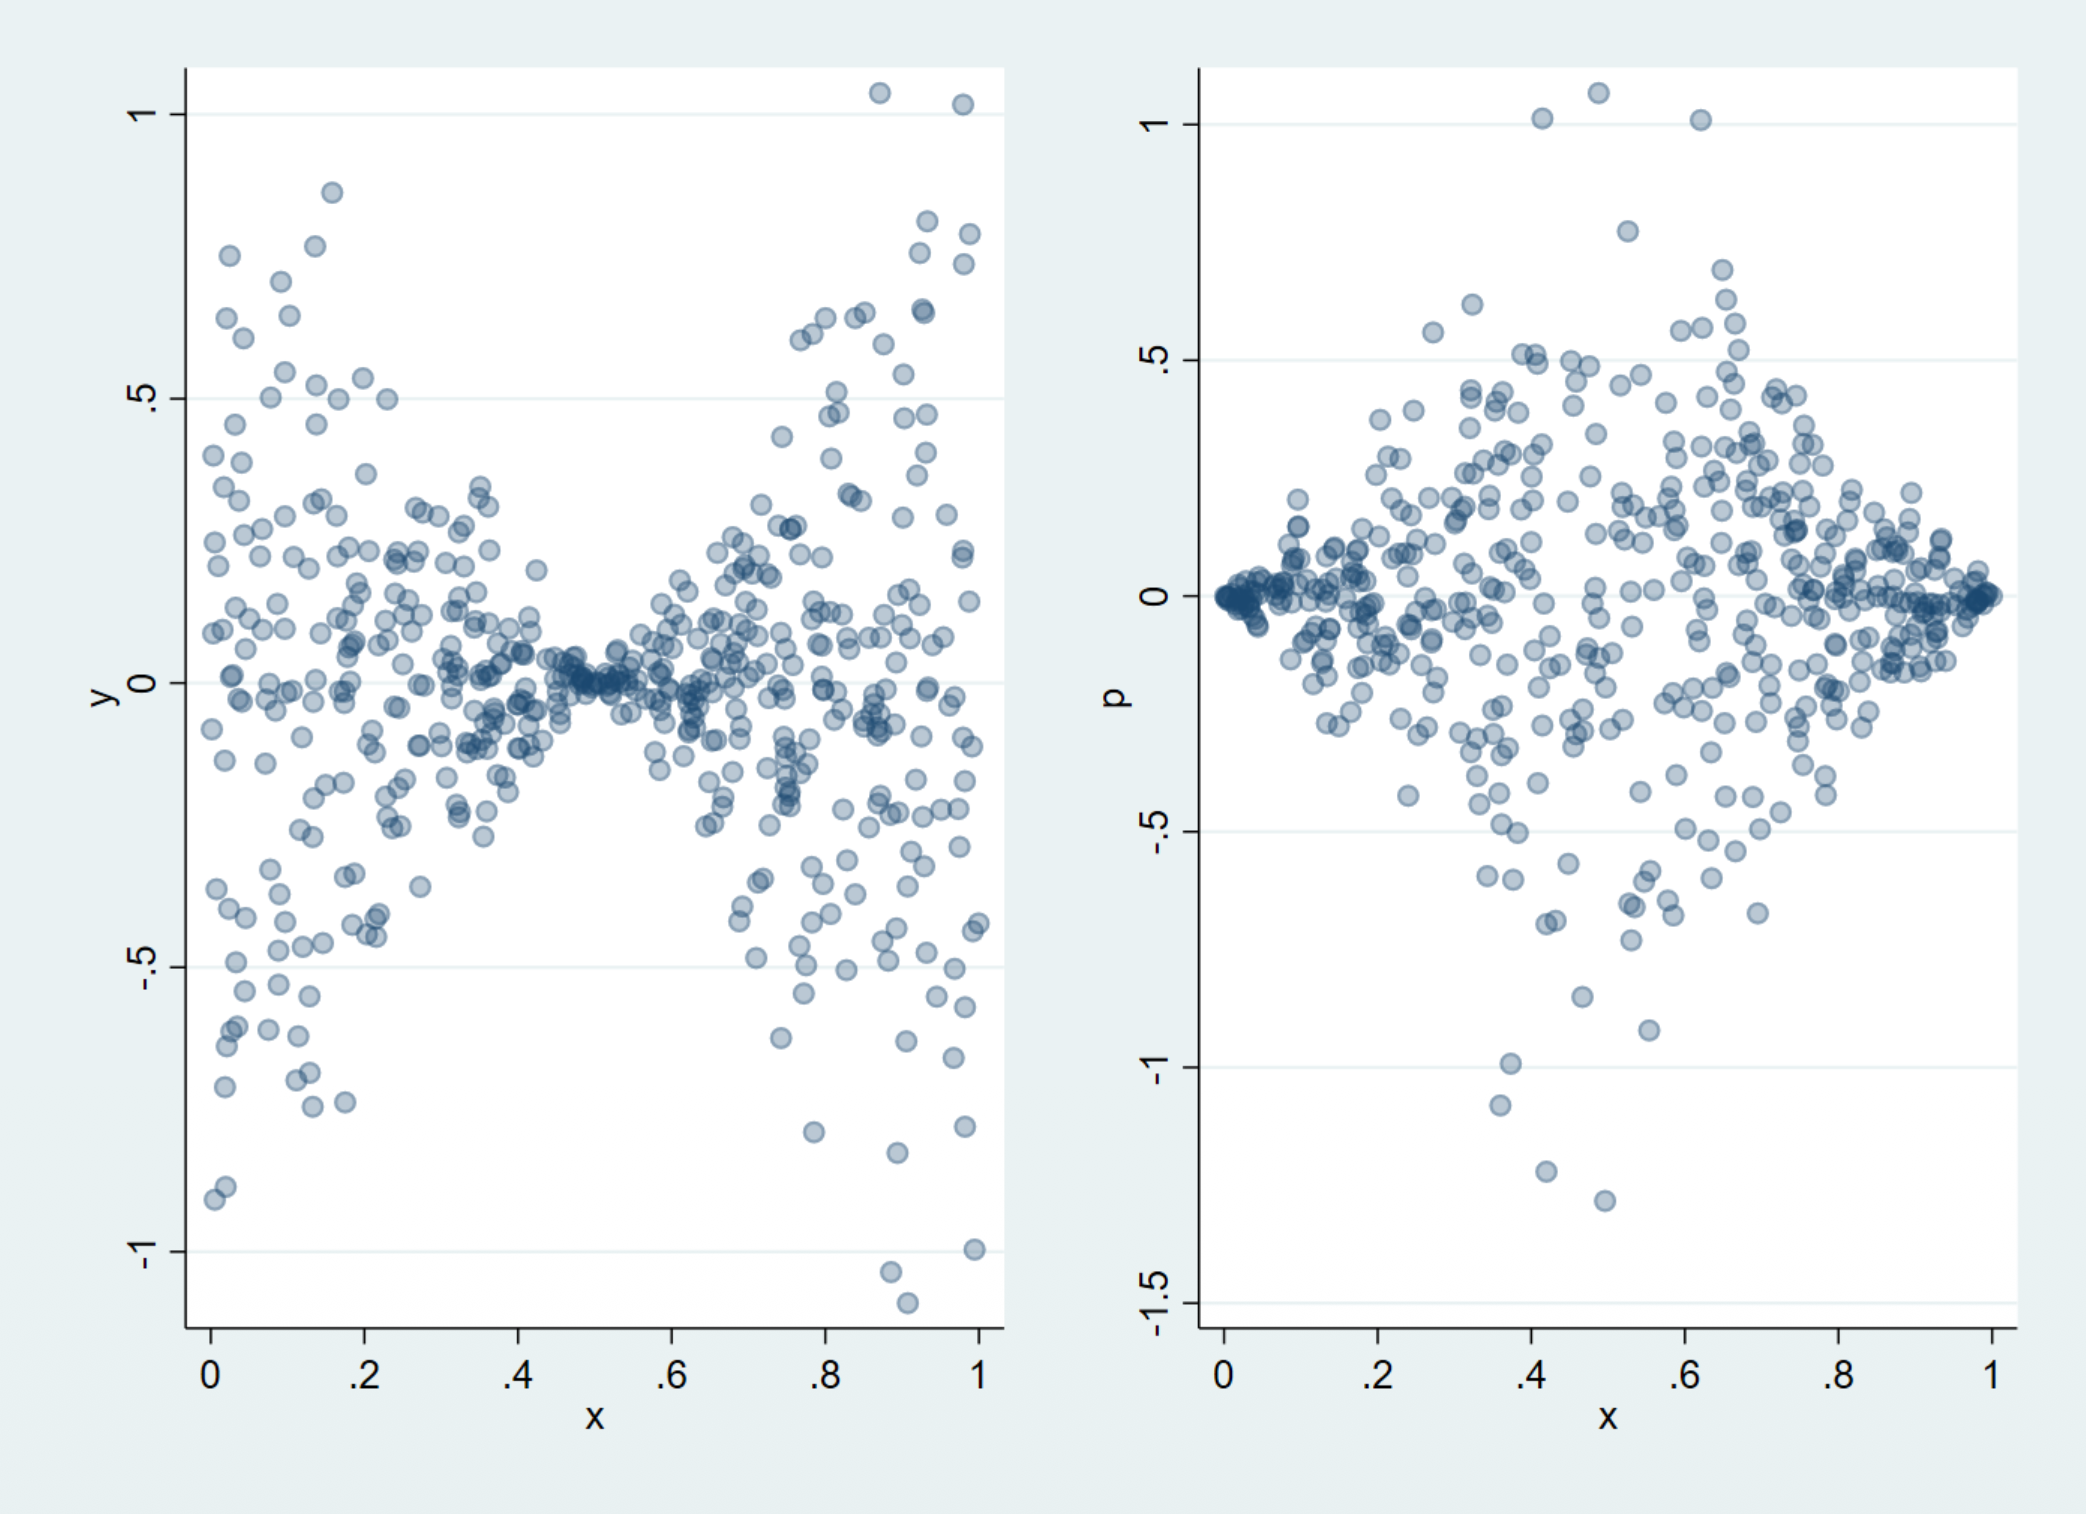
\includegraphics[width=0.78\textwidth]{images/2-12-1}
\end{figure}
Recalling a previous example, it should be much easier to estimate the slope $\beta_1$ from the data on the right, because the concentrations of mass are spread apart.
In fact, the heteroskedastic-robust standard error is smaller than the nonrobust standard error, so it is \emph{not} true that heteroskedastic-robust standard errors are always larger than nonrobust ones.

\begin{remark}	If MLR.5 holds: $\operatorname{Var}(u_i \mid x_i) = \sigma^2$. Since the error variance does not depend on the value of $x_i$, it is called homoskedastic.
	
	If the error variance depends on $x_i$, $u_i$ is heteroskedastic and MLR.5 fails.
	
	If MLR.1-4 are maintained, OLS is still unbiased and consistent under heteroskedasticity, but now the error variance depends on $x_i$: \[
		\operatorname{Var}(u_i \mid x_i) = \sigma_i^2
	,\] which in turn changes $\operatorname{Var}(\hat{\beta}_j \mid X)$.
\end{remark}

	\begin{remark}	If MLR.5 fails, and we use the wrong standard error, we may conclude that our result is significant because we mis-specified the variance of the estimator. This is why generalised least squares is not typically used and instead people do OLS with heteroskedasticity-robust standard errors (using the long form of asymptotic variance).

	Hence, while OLS will be unbiased and consistent, if we end up using the wrong test statistic in our hypothesis test, we may come to a wrong conclusion.

		We also note that using robust standard errors is valid when we have homoskedasticity, but we cannot use non-robust standard errors with heteroskedasticity. (Obviously, but we just need to emphasize this.) For example, consider the two regressions that use nonrobust and robust standard errors and the test statistic $\frac{\hat{\beta}_{\text{lotsize}}}{se\left( \hat{\beta}_{\text{lotsize}} \right)}$.
	\begin{figure}[htpb]
	  \centering
	  \begin{minipage}{0.49\textwidth}
	    \centering
	    \caption{Non-robust standard errors}
	    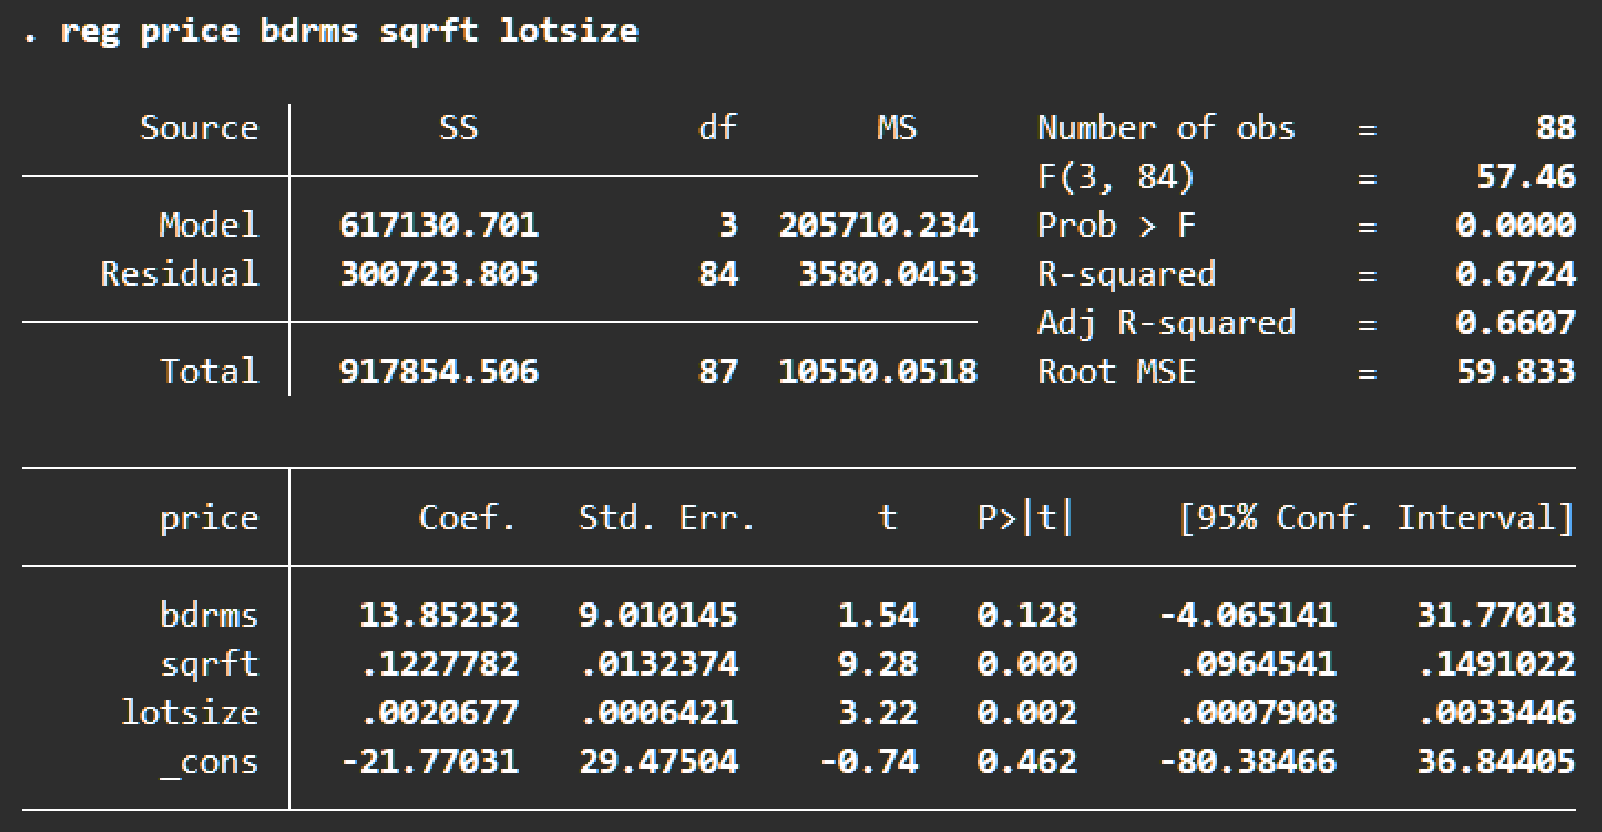
\includegraphics[width=\textwidth]{images/2-12-2}
	  \end{minipage}
	  \hfill
	  \begin{minipage}{0.49\textwidth}
	    \centering
	    \caption{Robust standard errors}
	    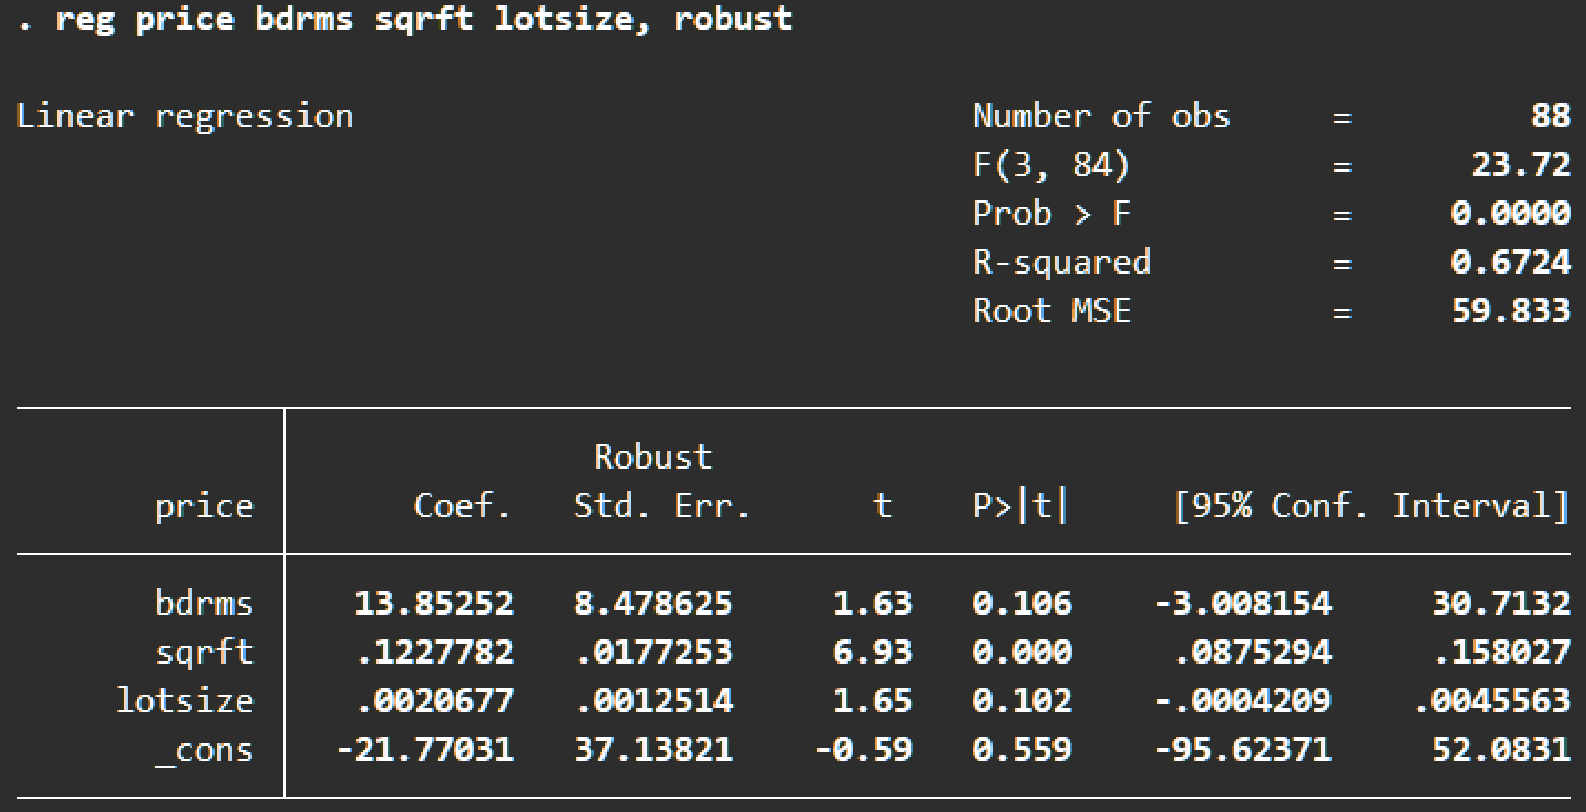
\includegraphics[width=\textwidth]{images/2-12-3}
	  \end{minipage}
	\end{figure}

	When would we ever use non-robust standard errors, then? 
	The advantage of non-robust standard errors is that $t$-stats have exact $t$-distributions under MLR.1-6.
	
	With robust standard errors, we need to use the approximation: \[
		\frac{\hat{\beta}_j - \beta_j}{\operatorname{se}_{\text{rob}}(\hat{\beta}_j)} \approx N(0,1)
	.\] 
	
	In practice, robust standard errors are used because they are valid with any form of heteroskedasticity, while justifying either of MLR.5 (homoskedasticity) or MLR.6 (normality of errors conditional on $X$) is difficult.
\end{remark}

	\begin{proposition}[Variance for individual coefficients]
		When $y_i = \beta_0 + \beta_1 x_{i1} + \cdots + \beta_k x_{ik} + u_i$, we find
		\begin{align*}
			\hat{\beta}_j = \left( X_j' M_{X_{-j}} X_j \right)^{-1} X_j' M_{X_{-j}} Y
		,\end{align*} so \[
			\hat{\beta}_j = \frac{\sum_{i=1}^{n} \hat{r}_{ij} y_i}{\sum_{i=1}^{n} \hat{r}_{ij}^2}
		,\] where $\hat{r}_{ij}$ denotes the $i$-th residual of a regression of $x_j$ on all other regressors.
	
	We find: \[
		\operatorname{Var}(\hat{\beta}_j \mid X) = \frac{\sum_{i=1}^{n} \hat{r}_{ij}^2 \operatorname{Var}(y_i \mid x_i)}{(\sum_{i=1}^{n} \hat{r}_{ij}^2)^2} = \frac{\sum_{i=1}^{n} \hat{r}_{ij}^2 \sigma_i^2}{(\sum_{i=1}^{n} \hat{r}_{ij}^2)^2}
	.\] 
	
	Because $\sigma_i^2$ is unknown, we replace it with $\E\left[u_i^2 \mid X_i\right] = \hat{u}_i^2$ and find: \[
		\widehat{\operatorname{Var}}(\hat{\beta}_j \mid X) = \frac{\sum_{i=1}^{n} \hat{r}_{ij}^2 \hat{u}_i^2}{(\sum_{i=1}^{n} \hat{r}_{ij}^2)^2}
	.\] 
	
	The heteroskedasticity robust standard error is given by\boxednote{Plugging $r_{i 1} = x_i - \overline{x}$ for a regression of $x_1$ onto a constant yields the expression we had in this section's exposition.} \[
		\operatorname{se}(\hat{\beta}_j) = \sqrt{\frac{\sum_{i=1}^{n} \hat{r}_{ij}^2 \hat{u}_i^2}{(\sum_{i=1}^{n} \hat{r}_{ij}^2)^2}}
	.\] 
\end{proposition}

\section{Weighted Least Squares}

\begin{proposition}[Weighted least squares transformation]
	If we knew the error variance $\sigma_i^2$, we could transform the model: \[
		\frac{y_i}{\sigma_i} = \left( \frac{1}{\sigma_i}, \frac{x_{i1}}{\sigma_i}, \ldots, \frac{x_{ik}}{\sigma_i} \right) \beta + \frac{u_i}{\sigma_i}
	.\] 

Notice that this model still satisfies MLR.4 since $\sigma_i$ only depends on $x_i$: \[
	\E\left( \frac{u_i}{\sigma_i} \mid x_i \right) = \frac{1}{\sigma_i} \E(u_i \mid x_i) = 0
.\] 

MLR.1-3 are unaffected, since multiplying each row of $X$ by a non-zero constant does not cause collinearity or change the interpretation of the model.

However, MLR.5 now holds, because \[
	\E\left[ \left( \frac{u_i}{\sigma_i} \right)^2 \mid \frac{x_i}{\sigma_i} \right] = \E\left[ \E\left[ \left( \frac{u_i}{\sigma_i} \right)^2 \mid x_i \right] \mid \frac{x_i}{\sigma_i} \right]
,\] and \[
	\E\left[ \left( \frac{u_i}{\sigma_i} \right)^2 \mid x_i \right] = \frac{1}{\sigma_i^2} \E(u_i^2 \mid x_i) = \frac{\sigma_i^2}{\sigma_i^2} = 1
.\] 

	OLS on the transformed model gives the best linear unbiased estimator of $\beta$ by the Gauss--Markov Theorem.\boxednote{There is some nuance here: Gauss--Markov gives us efficiency conditional on $\left(\frac{x_i}{\sigma_i}\right)$, but we will show in another problem set that it can be efficient conditional on $x$ as well.}
\end{proposition}

We really will just consider weighted least squares with homoskedasticity at the individual level. Geralized least squares weights based on the error variance, but this is beyond the scope of this course.

\begin{example}[WLS: Grouped Data]
	Suppose the model for observation $i$ is \[
		y_i = \beta_0 + \beta_1 x_i + u_i
	,\] where MLR.1-5 hold. Let $\operatorname{Var}(u \mid x) = \sigma^2$.
	
	Our observations are group averages e.g. mean age/income by zip code.
	
	There are $K$ groups $k = 1, \ldots, K$, and we observe \[
		\bar{y}_k = \frac{1}{n_k} \sum_{i \in \text{Group } k} y_i; \quad \bar{x}_k = \frac{1}{n_k} \sum_{i \in \text{Group } k} x_i
	\] for each $k = 1, \ldots, K$.
	
	We would actually run the regression on zip-code level data, so we make clear that the model written for averages is: \[
		\bar{y}_k = \beta_0 + \beta_1 \bar{x}_k + \bar{u}_k
	.\] 
	The error variance is \[
		\operatorname{Var}(\bar{u}_k \mid X) = \frac{\sigma^2}{n_k}
	.\] 
	This would actually give a different estimator of $\beta$ (since the weighting is uniform across zip codes, and not individuals as in the granular regression), and has heteroskedasticity.

	Hence, we should multiply by $\sqrt{n_k}$ to restore MLR.5\footnote{Note: we only recover homoskedasticity with this simple weighting because the original individual data was homoskedastic.} and estimate the following by OLS: \[
		\sqrt{n_k} \cdot \bar{y}_k = \beta_0 \cdot \sqrt{n_k} + \beta_1 \sqrt{n_k} \cdot \bar{x}_k + \sqrt{n_k} \cdot \bar{u}_k
	.\] 
	Here, $\operatorname{Var}(\sqrt{n_k} \cdot \bar{u}_k \mid X) = n_k \operatorname{Var}(\bar{u}_k \mid X) = \sigma^2$.
\end{example}

\section{Regression Specification}

\begin{remark}	Multiple linear regression can be used to model non-linear patterns in the data.
	
	We discuss:
	\begin{itemize}
		\item Using logarithms and polynomials to model non-linear patterns
		\item Turning continuous variables into qualitative variables
		\item Using qualitative variables to allow categories in the data to have their own coefficients
		\item Using interactions to allow the effect of changing one explanatory variable on the conditional mean to vary with the value of another.
	\end{itemize}
\end{remark}

\begin{remark}[Logarithms]
	Logarithms are often used to approximate proportional changes. For $x'$ close to $x$: \[
		\log(x') - \log(x) \approx \frac{x' - x}{x}
	\] by a first-order Taylor expansion, which is the proportional change from $x$ to $x'$.
	
	Several specifications used for conditional mean: \begin{align*}
		\E(y \mid x = t) &\approx \alpha + \beta \log(t) \quad \text{``level-log''} \\
		\E(\log(y) \mid x = t) &\approx \alpha + \beta t \quad \text{``log-level''} \\
		\E(\log(y) \mid x = t) &\approx \alpha + \beta \log(t) \quad \text{``log-log''}
	.\end{align*}
\end{remark}

Differentiating a conditional expectation is difficult, since we don't want to move the derivative operator in the expectation. Thus, the easiest log model to interpret is the log-level specification.

\begin{remark}[level-log specification]
	Consider $\E\left[y \mid x = t\right] = \alpha + \beta \ln{\left(t\right)}$.

	We have \begin{align*}
		\E(y \mid x = t + \Delta t) - \E(y \mid x = t) &\approx \beta[\log(t + \Delta t) - \log(t)] \\
		&\approx \beta \cdot \frac{\Delta t}{t} \\
		&= \frac{\beta}{100} \cdot \frac{100\Delta t}{t}
	,\end{align*} so $\beta/100$ is approximately the change in the conditional mean of $y$ when $t$ increases by $1\%$.\boxednote{This percentage interpretation is only valid for a causal interpretation, in that we examine a level of $t$ and error, then see the change in $y$ when increasing $t$. But we cannot differentiate a random variable with respect to another carelessly.}
\end{remark}

\begin{remark}[log-level specification]
	We have \[
		\E(\log(y) \mid x = t + 1) - \E(\log(y) \mid x = t) \approx \beta
	.\] 
	
		Expectations don't pass through non-linear functions (e.g. Jensen), but the following approximation leads to the common interpretation that a unit increase in $x$ is associated with a $\beta\%$ change in the mean of $y$:\boxednote{Jensen's inequality means $\E[\log y \mid x]$ need not equal $\log \E[y \mid x]$. The approximation is exact when $y \mid x$ is log-normal.} \begin{align*}
			\beta &\approx \E(\log(y) \mid x = t + 1) - \E(\log(y) \mid x = t) \\
			&\approx \log(\E(y \mid x = t + 1)) - \log(\E(y \mid x = t)) \\
			&\approx \frac{\E(y \mid x = t + 1) - \E(y \mid x = t)}{\E(y \mid x = t)}
	,\end{align*} so $100\beta$ is approximately the percentage change in the mean of $y$ resulting from a unit increase in $x$.
	
	Alternatively, exponentiating the first approximation and subtracting $1$ gives: \begin{align*}
		\exp(\beta) - 1 &\approx \exp(\E(\log(y) \mid x = t + 1) - \E(\log(y) \mid x = t)) - 1 \\
		&= \frac{\exp(\E(\log(y) \mid x = t + 1)) - \exp(\E(\log(y) \mid x = t))}{\exp(\E(\log(y) \mid x = t))}
	.\end{align*}
	Given that $\exp(x) \approx 1 + x$ when $x \approx 0$, the left hand side is approximately equal to $\beta$ if $\beta \approx 0$.
	
	We can therefore interpret $\beta$ as the proportional change in the conditional geometric mean of $y$ given a unit increase in $x$, holding the error term fixed.
\end{remark}

\begin{remark}[log-log specification]
	Now we have \[
		\E(\log(y) \mid x = t + \Delta t) - \E(\log(y) \mid x = t) \approx \beta[\log(t + \Delta t) - \log(t)]
	.\] 
	
	Combining the approximations for log-level and level-log gives: \[
		\frac{\E(y \mid x = t + \Delta t) - \E(y \mid x = t)}{\E(y \mid x = t)} \approx \beta \cdot \frac{\Delta t}{t}
	,\] so a $1\%$ increase in $t$ is associated with a $\beta\%$ change in the conditional mean of $y$ (also known as an elasticity).
\end{remark}

\begin{example}[Returns to experience]
	Consider the approximation: \[
		\E(\text{wage} \mid \text{exper}) \approx \beta_0 + \beta_1 \text{exper} + \beta_2 \text{exper}^2
	.\] 
	
	Experience estimated to have a diminishing marginal effect on wage.
	
	Turning point estimated where \[
		\frac{\partial \E(\text{wage} \mid \text{exper} = e^*)}{\partial e} = \hat{\beta}_1 + 2\hat{\beta}_2 e^* = 0 \implies e^* = -\frac{\hat{\beta}_1}{2\hat{\beta}_2} \approx 24
	.\] 
\end{example}

\begin{remark}[Returns to Experience]
	Issues with a causal interpretation:
	\begin{itemize}
		\item Omitted Variables Bias: Education impacts wage and may be correlated with/interact with exper or exper$^2$.
		\item Functional form misspecification: $w$ or $\ln(w)$? Quadratic in experience?
	\end{itemize}
	
	Average partial effect: What is the marginal effect of experience? \[
		\frac{\partial \E(\text{wage} \mid \text{exper} = e)}{\partial e} = \beta_1 + 2\beta_2 e
	.\] 
	The effect of experience diminishes if $\beta_2 < 0$. We can estimate the average partial effect: \[
		\widehat{\text{APE}} = \frac{1}{n} \sum_{i=1}^{n} (\hat{\beta}_1 + 2\hat{\beta}_2 \text{exper}_i) = \hat{\beta}_1 + 2\hat{\beta}_2 \overline{\text{exper}}_n
	.\] 
\end{remark}

\begin{remark}[Dummy Variables]
	Suppose we want to measure the difference in average wages between the tech industry and all other industries.
	
	Use a ``Dummy Variable'' to denote categories within data.
\end{remark}

\begin{remark}[Continuous variables to categorical variables]
	Suppose we are interested in estimating store sales by age category:
	\begin{itemize}
		\item Observe sales figures and age of customers.
		\item Create $k$ categories as follows: \[
			d_{i1} = \begin{cases}
				1 & \text{if } i \text{ is between 0-18 years of age} \\
				0 & \text{otherwise}
			\end{cases}
		\] \[
			d_{i2} = \begin{cases}
				1 & \text{if } i \text{ is between 18-25 years of age} \\
				0 & \text{otherwise}
			\end{cases}
		\] \[
			\vdots
		\] \[
			d_{ik} = \begin{cases}
				1 & \text{if } i \text{ is 75+ years of age} \\
				0 & \text{otherwise}
			\end{cases}
		\] 
	\end{itemize}
	
	Note: Groups are mutually exclusive ($d_{ij} d_{ik} = 0$ when $i \ne j$) and exhaustive ($d_{i1} + \cdots + d_{ik} = 1$).
	
	Means WLOG we can describe average sales by age category using \[
		\E(y_i \mid d_{i1}, \ldots, d_{ik}) = \beta_1 d_{i1} + \beta_2 d_{i2} + \cdots + \beta_k d_{ik}
	,\] where intercept is excluded to avoid perfect collinearity.
	
	Can also specify \[
		\E(y_i \mid d_{i1}, \ldots, d_{ik}) = \alpha_0 + \alpha_1 d_{i1} + \alpha_2 d_{i2} + \cdots + \alpha_{k-1} d_{ik-1}
	.\] 
	
	Note: \[
		\alpha_1 = \E(y \mid d_{i1} = 1, \ldots, d_{ik} = 0) - \E(y \mid d_{i1} = 0, \ldots, d_{ik} = 1)
	\] is interpreted as the difference in average spend between the youngest and oldest age categories.
	
	Excluding the dummy variable for the oldest category specifies that category as the base group.
	
	Intercept $\alpha_0$ is the mean for the base group.
	
	$\alpha_j$ represents difference in means between group $j$ and base group.
\end{remark}

\begin{remark}[Kinks and Jumps]
	Describe credit limits offered to new customers as a function of credit score.
	
	Sometimes outcome will change sharply at a cutoff. Suppose $y$ is credit limit and $x$ is credit score.
	
	Suppose only two categories of credit: 'Good' and 'Excellent'.
	
	Features:
	\begin{itemize}
		\item Sharp discontinuity in credit limit as soon as individual crosses 'Excellent' boundary
		\item Each additional unit of credit score improves credit limit more for individuals with excellent credit (Kink)
	\end{itemize}
	
	Let \[
		d_i = \begin{cases}
			1 & \text{if individual } x_i \ge 0.5 \\
			0 & \text{if individual } x_i < 0.5
		\end{cases}
	\] 
	
	Model: \begin{align*}
		y_i &= \beta_0 + \beta_1 x_i + d_i(\gamma + \delta x_i) + \epsilon_i \\
		&= \beta_0 + \beta_1 x_i + \gamma d_i + \delta d_i x_i + \epsilon_i
	.\end{align*}
	
	When $x_i < a$: $\E(y_i \mid x = x_i) = \beta_0 + \beta_1 x_i$.
	
	When $x_i \ge a$: $\E(y_i \mid x = x_i) = (\beta_0 + \gamma) + (\beta_1 + \delta) x_i$.
	
	Note: not all parameters have a useful interpretation: $\beta_0 + \gamma$ is the credit limit an individual with 'Excellent' credit would receive if their credit score were $0$ (We could never observe such individuals in the data).
	
	$\delta$ represents the additional return to credit score for individuals with excellent credit.
	
	Jump: $\gamma + \delta \cdot 0.5$.
\end{remark}

\begin{remark}[Saturated Regression]
	Describe wages in tech vs. not in tech, both inside and outside california: \[
		\E(W \mid T, C) = \beta_0 + \beta_1 T + \beta_2 C + \beta_3 T \cdot C
	.\] 
	We call this a saturated regression since it has one parameter for each possible value of the regressors: \[
		(T, C) \in \{(0,0), (1,0), (0,1), (1,1)\}
	.\] 
	
	The equality holds by construction, not because of an additional assumption about linearity of the conditional mean.
	
	Could also specify \[
		\E(W \mid T, C) = \alpha_0 (1-T) \cdot (1-C) + \alpha_1 T \cdot (1-C) + \alpha_2 (1-T) \cdot C + \alpha_3 T \cdot C
	.\] 
	
	Only difference is in interpretation of parameters: \begin{align*}
		\E(W \mid T = 0, C = 0) &= \beta_0 = \alpha_0 \\
		\E(W \mid T = 1, C = 0) &= \beta_0 + \beta_1 = \alpha_1 \\
		\E(W \mid T = 0, C = 1) &= \beta_0 + \beta_2 = \alpha_2 \\
		\E(W \mid T = 1, C = 1) &= \beta_0 + \beta_1 + \beta_2 + \beta_3 = \alpha_3
	.\end{align*}
	
	$\beta_1$ represents difference in average wages in tech vs. not for employees outside california.
	
	$\beta_2$ represents difference in average wages in california vs. not for employees not in tech.
	
	$\beta_3$ represents a ``difference in differences''. For example: \begin{align*}
		\beta_3 &= [(\beta_0 + \beta_1 + \beta_2 + \beta_3) - (\beta_0 + \beta_2)] - [(\beta_0 + \beta_1) - \beta_0] \\
		&= [\E(W \mid T = 1, C = 1) - \E(W \mid T = 0, C = 1)] \\
		&\quad - [\E(W \mid T = 1, C = 0) - \E(W \mid T = 0, C = 0)]
	.\end{align*}
	
	This is the difference (between california and not) in differences in wages inside and outside tech.
\end{remark}

	\begin{remark}[Interactions]
		An interaction is a product of two regressors. e.g. \[
			\text{wage} = \beta_0 + \beta_1 \text{educ} + \beta_2 \text{exper} + \beta_3 \text{educ} \cdot \text{exper} + \epsilon
	.\] 
	
		If $\E(\epsilon \mid \text{educ}, \text{exper}) = 0$, we have: \[
			\frac{\partial}{\partial \text{exper}} \E(\text{wage} \mid \text{educ}, \text{exper}) = \beta_2 + \beta_3 \text{educ}
		,\] so if $\beta_3 > 0$, average wage for those with more education differs more across experience levels.
	\end{remark}

\section{Summary}

\begin{remark}[Model and estimator]
	\leavevmode\hfill\break
	\textbf{Model}: $y = x'\beta + u$ with $\E\left[xu\right] = 0$. \\
	\textbf{Estimator}: $\hat{\beta}^{OLS} = (X'X)^{-1}X'Y$. \\
	\textbf{Interpretation}: each coefficient is the slope of the conditional mean with the remaining regressors held fixed.
\end{remark}

\begin{remark}[Finite-sample inference under normality]
	Suppose $Y \mid X \sim N(X\beta,\sigma^2 I_n)$. Exact conditional distributions:
	\[
		\begin{aligned}
			\hat{\beta} \mid X &\sim N\left(\beta,\sigma^2 (X'X)^{-1}\right), \\
			\hat{\sigma}^2 = \frac{SSR}{n-k} &\sim \frac{\sigma^2}{n-k}\chi^2_{n-k}
		\end{aligned}
	.\]
	The key finite-sample fact is that $\hat{\beta}-\beta$ and $\hat{\sigma}^2$ are conditionally independent, which yields exact $t_{n-k}$ tests and confidence intervals.
\end{remark}

\begin{remark}[Large-sample inference]
	Without normality, asymptotic normality replaces exact finite-sample formulas:
	\[
		\sqrt{n}(\hat{\beta}_n-\beta) \xrightarrow{d} N(0,V)
	.\]
	Single restrictions use asymptotic $z$-tests and confidence intervals, while multiple restrictions use $\chi^2_p$ statistics and ellipsoidal confidence sets for $R\beta$.
\end{remark}

\begin{remark}[Homoskedastic vs.\ heteroskedastic inference]
		\begin{center}
		\small
		\renewcommand{\arraystretch}{1.1}
		\begin{tabular}{p{0.20\linewidth}p{0.27\linewidth}p{0.33\linewidth}}
			\toprule
			Case & Standard error formula & Inference to use \\
			\midrule
			Homoskedastic, normal & $\hat{\sigma}^2(X'X)^{-1}$ & Exact $t$ / exact finite-sample \\
			Homoskedastic, large sample & $\hat{\sigma}^2(X'X)^{-1}$ & Asymptotic normal / $\chi^2$ \\
			Heteroskedastic & $(X'X)^{-1}X'\hat{\Omega}X(X'X)^{-1}$ & Robust asymptotic normal / $\chi^2$ \\
			\bottomrule
		\end{tabular}
		\end{center}
		Robust standard errors are valid in both homoskedastic and heteroskedastic settings, but exact $t$ inference requires the stronger homoskedastic-normal setup.
\end{remark}

\begin{remark}[Weighted least squares]
	If $\operatorname{Var}(u_i \mid x_i) = \sigma_i^2$ is known, divide the $i$-th observation by $\sigma_i$ to restore homoskedasticity. OLS on the transformed model is WLS and is efficient within the class of linear unbiased estimators under the transformed homoskedastic model.
\end{remark}

\begin{remark}[Regression specifications]
	Common specifications and their interpretation:
	\begin{itemize}
		\item \textbf{Level-log}: $\beta/100$ is the change in $\E(y \mid x)$ for a $1\%$ increase in $x$.
		\item \textbf{Log-level}: $100\beta$ approximates the percent change in $\E(y \mid x)$ for a one-unit increase in $x$.
		\item \textbf{Log-log}: $\beta$ is an elasticity.
		\item \textbf{Dummies/interactions}: allow group-specific intercepts, slopes, and difference-in-differences style comparisons.
	\end{itemize}
\end{remark}

\styledchapter{Selection on Observables}

\begin{remark}	So far we have considered counterfactuals using linear regression:
	\begin{itemize}
		\item How much does earnings potential increase with another year of experience, holding all else fixed?
		\item How much does an additional bedroom increase house price, holding floor area/lot size/air pollution (and all else) fixed?
	\end{itemize}
	OLS estimates proportional to ``partial correlations'' between outcome and regressors. ``Holding fixed'' other observable factors in this way answers counterfactual question if $y = x'\beta + u$ and $\E\left[xu\right] = 0$. In particular, $\E\left[xu\right] = 0$ implies
	\[
		\beta = \E\left[xx'\right]^{-1}\E\left[xy\right]
	,\]
	so (scaled) partial correlations are partial (causal) effects, and scaled partial correlations can be estimated.
\end{remark}

\begin{definition}[Rubin Causal Model]
	We can think about counterfactuals as `potential outcomes' under different `treatments':
	\begin{itemize}
		\item Earnings with college degree, $y(1)$, and without $y(0)$.
		\item Health outcome with drug A, $y(1)$, vs. drug B, $y(0)$.
		\item Productivity with job training, $y(1)$ vs. without, $y(0)$.
	\end{itemize}
	Define individual treatment effect for individual $i$ as $y_i(1) - y_i(0)$. Denote treatment status of individual $i$ by $D_i \in \left\{0, 1\right\}$.
\end{definition}

\section{Motivation: Store Upgrades}

Consider $100$ stores where we are trying to measure the effect of receiving an interior upgrade on sales.

\begin{example}[Store Upgrades]
	$y_i(1)$ denotes sales store $i$ would observe with an upgrade. $y_i(0)$ denotes sales store $i$ would observe without an upgrade. The outcome observed is
	\[
		Y_i =
		\begin{cases}
			y_i(1) & \text{if store $i$ is upgraded,} \\
			y_i(0) & \text{if not.}
		\end{cases}
	\]
	In other words,
	\[
		Y_i = y_i(1)D_i + y_i(0)\left(1-D_i\right)
	,\]
	where $D_i$ is an indicator for if store $i$ received an upgrade.

	We never observe the individual causal effect $y_i(1)-y_i(0)$ for any store because only one of the two potential outcomes is ever observed. However, we can try to measure average effects across treated and untreated stores by comparing averages:
	\begin{itemize}
		\item e.g. Average Treatment Effect in store population (ATE): $\E\left[y(1)-y(0)\right]$.
		\item e.g. Average Treatment Effect on the treated (ATT): $\E\left[y(1)-y(0) \mid D=1\right]$.
		\item e.g. Average Treatment Effect on untreated (ATU): $\E\left[y(1)-y(0) \mid D=0\right]$.
	\end{itemize}

	What is identified from $\E\left[Y \mid D\right]$?

	First write out the conditional mean of $Y \mid D$:
	\begin{align*}
		\E\left[Y \mid D=1\right] &= \E\left[y(1)D + y(0)(1-D) \mid D=1\right] \\
		&= \E\left[y(1) \mid D=1\right] \\
		\E\left[Y \mid D=0\right] &= \E\left[y(1)D + y(0)(1-D) \mid D=0\right] \\
		&= \E\left[y(0) \mid D=0\right]
	.\end{align*}
	We can observe $\E\left[y(1) \mid D=1\right]$ and $\E\left[y(0) \mid D=0\right]$. The data reveal an estimate of the `naive comparison':
	\[
		\E\left[y(1) \mid D=1\right] - \E\left[y(0) \mid D=0\right]
	,\]
	which is ATT plus selection effects.
\end{example}

\begin{remark}    Examining stores that are upgraded, not upgraded, and the whole population, we might see that
	\begin{center}
		\scriptsize
		\renewcommand{\arraystretch}{1.15}
		\begin{tabular}{p{0.24\linewidth}p{0.18\linewidth}p{0.18\linewidth}p{0.18\linewidth}}
			& $D_i = 0$ & $D_i = 1$ & All \\
			\hline
			average sales if upgraded
				& $\E[y(1)\mid D=0]=?$ 
				& $\E[y(1)\mid D=1]=100$
				& $\E[y(1)]=?$ \\
			average sales if not upgraded
				& $\E[y(0)\mid D=0]=50$
				& $\E[y(0)\mid D=1]=?$
				& $\E[y(0)]=?$ \\
			difference
				& $\E[y(1)-y(0)\mid D=0]=ATU$
				& $\E[y(1)-y(0)\mid D=1]=ATT$
				& $\E[y(1)-y(0)]=ATE$
		\end{tabular}
	\end{center}
\end{remark}

\begin{proposition}[Relationship between ATE, ATT, ATU]
	We can decompose the ATE as follows:
		\begin{align*}
			\E\left[y(1)-y(0)\right]
			&= \E\left[y(1)-y(0) \mid D=1\right]\P\left(D=1\right) \\
			&\quad + \E\left[y(1)-y(0) \mid D=0\right]\P\left(D=0\right) \\
			&= ATT \cdot \P\left(D=1\right) + ATU \cdot \P\left(D=0\right)
		.\end{align*}
\end{proposition}
\begin{proof}
	By the law of iterated expectation.
\end{proof}

\begin{proposition}[Regression and selection bias]
	Write out the conditional mean of $Y \mid D$:
	\[
		\E\left[Y \mid D=1\right] = \E\left[y(1) \mid D=1\right], \qquad
		\E\left[Y \mid D=0\right] = \E\left[y(0) \mid D=0\right]
	.\]
	It follows that
	\[
		\E\left[Y \mid D\right] = \beta_0 + \beta_1 D
	,\]
	where
	\[
		\beta_0 = \E\left[y(0) \mid D=0\right], \qquad
		\beta_1 = \E\left[y(1) \mid D=1\right] - \E\left[y(0) \mid D=0\right]
	.\]
\end{proposition}
\begin{proof}
	Thus $\beta_1$ equals the naive comparison. Moreover,
	\begin{align*}
		\beta_1
		&= \E\left[y(1) \mid D=1\right] - \E\left[y(0) \mid D=0\right] \\
		&= \underbrace{\E\left[y(1) \mid D=1\right] - \E\left[y(0) \mid D=1\right]}_{\text{ATT}}
		+ \underbrace{\E\left[y(0) \mid D=1\right] - \E\left[y(0) \mid D=0\right]}_{\text{Selection Bias}}
	.\end{align*}
		$\beta_1$ measures the average effect on stores that were upgraded (ATT) but is offset by ``selection bias'' in $y(0)$, which measures differences in average sales in the absence of upgrades.\boxednote{Equivalent decompositions are $\beta_1=ATT+SB_{y(0)}$ and $\beta_1=ATU+SB_{y(1)}$.}
\end{proof}

\begin{remark}	There is a big difference between selection bias in $y(0)$ vs selection bias in $y(1)$.
	
	For selection bias in $y(0)$ but not in $y(1)$, consider factories that do not get training who have scrap rates of $0.01$, factories that do get training who initially have scrap rates of $0.05$, but then $0.01$ after training.

	For selection bias in $y(1)$ but not $y(0)$, consider factories all with the same scrap rate, then factory managers who only opt into training if their employees are trainable, whose scrap rates go down after treatment. If the factories who opted out of training would have had the same scrap rate as before even if they received training, we would have selection bias in $y(1)$ only.

	Furthermore, the naive comparison can equal the ATE if the probability of selection and the magnitude of ATT/ATU cancel each other out, but this is generally not the case.
\end{remark}

\section{Random assignment}

\begin{definition}[Random assignment]
	How treatment is assigned determines whether selection bias is present. Random assignment:
	\[
		D_i \ind \left(y_i(0), y_i(1)\right)
	.\]
	This says treatment choice/assignment is independent of outcomes under treatment and no treatment.
\end{definition}

\begin{proposition}[Random assignment implies $\beta_1 = ATE$]
	Under random assignment,
	\[
		\E\left[y(0) \mid D\right] = \E\left[y(0)\right], \qquad
		\E\left[y(1) \mid D\right] = \E\left[y(1)\right]
	,\]
	i.e.\ the treatment and control groups are representative of the entire population. Hence,
	\[
		\beta_1 = \E\left[y(1)\right] - \E\left[y(0)\right] = ATE
	.\]
\end{proposition}
\begin{proof}
	\begin{align*}
		\beta_1
		&= \E\left[y(1) \mid D=1\right] - \E\left[y(0) \mid D=0\right] \text{ (naive comparison)}\\
		&= \E\left[y(1)\right] - \E\left[y(0)\right] \\
		&= ATE
	.\end{align*}
	Hence, under randomized treatment assignment, estimating a linear regression (which gives a coefficient that is the naive estimator) produces an unbiased estimate of the ATE.
\end{proof}

\begin{remark}[Multiple possible treatments]
	Suppose in a randomized clinical trial there is a control group and $k$ possible treatments for a particular health condition. Suppose participants are randomly assigned to either control or one of the treatments. Let
	\[
		x_{i1} =
		\begin{cases}
			1 & \text{if $i$ receives treatment 1,} \\
			0 & \text{otherwise,}
		\end{cases}
		\qquad
		x_{i2} =
		\begin{cases}
			1 & \text{if $i$ receives treatment 2,} \\
			0 & \text{otherwise,}
		\end{cases}
	\]
	and similarly for $x_{ik}$. There are now $k+1$ potential outcomes $y_i(0), y_i(1), \ldots, y_i(k)$ and
	\[
		Y_i = y_i(0) + x_{i1}\left(y_i(1)-y_i(0)\right) + \cdots + x_{ik}\left(y_i(k)-y_i(0)\right)
	.\]
	Now let $x_i = \left(1, x_{i1}, \ldots, x_{ik}\right)'$. We have
	\[
		\E\left[Y_i \mid x_i\right] = \beta_0 + \beta_1 x_{i1} + \cdots + \beta_k x_{ik}
	,\]
	where $\beta_0 = \E\left[y(0)\right]$ and, for each $j = 1, \ldots, k$, $\beta_j = \E\left[y(j)-y(0)\right]$.

	If we have random assignment, 
	\begin{align*}
		\E\left[Y_i \mid x_{i,1} = 0,\ldots,x_{i,k} = 0\right] &= \E\left[y_i(0) \mid x_{i,1} = 0 ,\ldots, x_{i,k} = 0\right] = \E\left[y_i(0)\right] \\
		\E\left[Y_i \mid x_{i,1} = 0 ,\ldots,x_{i,k} = 1\right] &= \E\left[y_i(k) \mid x_{i,1}= 0,\ldots,x_{i,k} = 1\right] = \E\left[y_i(k)\right] 
	.\end{align*}

	We can test whether these effects are statistically different from zero (or from each other) by forming appropriate hypotheses, e.g. $H_0:\beta_k=0$ or $H_0:\beta_1=\beta_2$.
\end{remark}

\section{Nonrandom assignment}

Now we examine when we don't have random assignment and in fact have selection bias.

\begin{example}[Job Training]
	JTRAIN98 contains data on labor market outcomes for men, some of whom enrolled in a job training program in 1997. Only men who had low earnings were allowed to enroll in the program:

	Considering the potential outcomes of earnings in 1998 without and with training, we see that the potential outcomes are correlated with treatment, because those who were eligible to be treated were lower income to begin with. (We expected both potential outcomes to be negatively correlated with $D$.) But conditioning on earnings in 1996 may remove this.

	\begin{itemize}
		\item Whether or not individual took training in 1997: $train = 1$ if training taken
		\item Earnings in 1998 (in \$1000s): $earn98$
		\item Earnings in 1996 (in \$1000s): $earn96$
		\item Whether or not individual is married: $married = 1$ if married
		\item Education in years of schooling: $educ$
		\item Age in years: $age$
	\end{itemize}
	First, compute naive comparison by running regression:
	\[
		earn98 = \beta_0 + \beta_1 train + \epsilon
	.\]Then $\hat{\beta}_1 = \overline{y}_{train} - \overline{y}_{not train} \xrightarrow{p} \E\left[Y \mid D = 1\right] - \E\left[Y \mid D = 0\right] $.
	$\hat{\beta}_1$ is a comparison of means between individuals who did/did not take training, and indicates that individuals who took training earned \$2050 less on average in 1998. This is because the selection bias is outweighing the treatment effect.

	Or, controlling for observable characteristics:
	\[
		earn98 = \beta_0 + \beta_1 train + \beta_2 educ + \beta_3 age + \beta_4 married + \beta_5 earn96 + \epsilon
	.\]

	The regression results show a negative coefficient on training when not controlling for observable characteristics, but a statistically significant positive coefficient on training when controlling for observable characteristics.
\end{example}
\begin{definition}[Covariate balance test]
	One way random assignment is justified statistically is by a ``balance test.'' We want to see if individuals with particular covariates are more likely to select into treatment. Practically: Regress treatment dummy $D_i$ on observable characteristics $x_i$:
	\[
		D_i = \gamma_0 + x_i'\gamma_1 + \epsilon_i
	.\]
	Conduct $F$-test of $H_0:\gamma_1=0$ vs. $H_1:\gamma_1 \ne 0$.\boxednote{The $F$-test is the finite sample analog of the test of multiple linear restrictions ($t$-test vs. $z$-test).}
\end{definition}

\begin{remark}[Issues with balance tests]
	The goal of a balance test is to show that $D$ is independent of potential outcomes. But this is not something that is measurable.
	A balance test can show that $x$ is uncorrelated with potential outcomes, but this is not the same thing. Both directions can fail --- there may be unobserved factors that are causally linked to the outcome, while some observables may be correlated with the outcome but have no causal relationship.

	If the significance level is 5\%, we will reject $H_0$ 5\% of the time even when $\gamma_1 = 0$. This means calling into question validity of 5\% of experimental results. If the balance test fails to reject, it doesn't mean randomization holds. $D_i$ may just be independent of observed covariates, leading to $\gamma_1 = 0$. What is really needed is
	\[
		D_i \ind \left(y_i(0), y_i(1)\right)
	.\]
\end{remark}

\begin{definition}[Unconfounded treatment assignment]
	Treatment assignment is unconfounded if, conditional on observed covariates $x_i$, treatment is as good as randomly assigned:
	\[
		D_i \ind \left(y_i(0), y_i(1)\right) \mid x_i
	.\]
	By this, we mean \[
		\P\left[D \in A, \left( y(0),y(1) \right) \in B \mid X\right] = \P\left[D \in A \mid X\right] \P\left[\left( y(0),y(1) \right) \in B \mid X\right] 
	\] for any events $A,B$. Conditional independence does not imply independence, and the converse is not true either.
\end{definition}

\begin{remark}[Conditioning on too much]
	Conditioning on too much (adding more covariates) is not always a good thing. Sometimes people argue that as long as you include all of the ``right'' covariates such that $D_i \ind \left( y_i(0), y_i(1) \right) \mid x_i$, you can add more covariates and maintain independence. But this is not true --- consider $X_{n+1}$ determining treatment assignment.
	Some machine learning fans are disappointed by this.
\end{remark}
	
\begin{example}[Selection on observables]
	Consider $W$ as earnings potential (wage) and $D = \mathds{1}_{\text{employed}}$. If we assume $W \ind D$, then $F_W(\cdot \mid D=1) = F_W(\cdot \mid D=0)$, so we could measure the population distribution of earnings potential by just looking at wages of the employed individuals.

	Now, consider a situation with a reservation wage $R$ such that $D = 1 \iff W \ge R$. Then if everyone has the same reservation wage, this independence obviously does not hold. Suppose the reservation wage is not identical and independence still holds.
	Then 
	\begin{align*}
		\E\left[W \mid D = 1, R = r\right] &= \E\left[W \mid W \ge R , R= r\right]  \\
											&= \E\left[W \mid W \ge r, R = r\right] \ge r\\
		\E\left[W \mid D=0, R = r\right]  &= \E\left[W \mid W < r, R = r\right] \\
										  &< r
	.\end{align*}
	We see that missingness at random does not imply missingness at random conditional on reservation wage. In other words, unconfoundedness may fail to hold if we condition on too much.
	
\end{example}

\begin{proposition}[Selection on observables via linear regression]
	Unconfounded treatment assignment implies
	\[
		\E\left[y(1) \mid D, x\right] = \E\left[y(1) \mid x\right], \qquad
		\E\left[y(0) \mid D, x\right] = \E\left[y(0) \mid x\right]
	,\]
	so we can estimate $\E\left[y(1) \mid D=1, x\right]$ and $\E\left[y(0) \mid D=0, x\right]$ and then estimate the ATE by aggregating over $x$.
\end{proposition}
\begin{proof}
	We see that 
	\begin{align*}
		ATE
		&= \E\left[y(1) - y(0)\right] \\
		&\overset{\text{LIE}}{=} \E\left[\E\left[y(1) - y(0) \mid X\right] \right] \\
		&= \E\left[\E\left[y(1) \mid X\right] - \E\left[y(0) \mid X\right] \right] \\
		&= \E\left[\E\left[y(1) \mid D=1,X\right] - \E\left[y(0) \mid D =0 , X\right] \right]  \text{ by unconfoundedness} \\
		&= \E\left[\E\left[Y \mid D = 1 , X\right] - \E\left[Y \mid D = 0, X\right] \right]
	.\end{align*}
	So if we can estimate $\E\left[Y \mid D=1, X\right] $, $\E\left[Y \mid D=0, X\right] $, and $F_X$, then we can estimate the ATE.
		Note that this expression is not the naive comparison, because\boxednote{The weights differ:
		$\E[Y \mid D=1]$ uses $\P(X=x \mid D=1)$, while $\E[\E[Y \mid D=1,X]]$ uses the unconditional distribution of $X$.} \[
			\E\left[Y \mid D= 1\right]  \ne \E\left[\E\left[Y \mid D=1 ,X\right] \right] 
		.\] 

	We approximated conditional means with a linear model
	\[
		\E\left[Y_i \mid D_i, x_i\right] \approx \beta_0 + \beta_1 D_i + x_i'\beta_2
	.\]
	This approximation gives
	\[
		\E\left[Y \mid D=1, x\right] - \E\left[Y \mid D=0, x\right] \approx \beta_1
	.\]
	The LIE implies that $\beta_1 = \E\left[y(1)-y(0)\right]$ (which is the ATE).

		The approximation works if\boxednote{This imposes common slopes across treated and untreated groups. It is convenient, but not necessary, for identification.}
		\[
			\E\left[y(0) \mid x\right] = \alpha_0 + x'\beta_2, \qquad
			\E\left[y(1) \mid x\right] = \alpha_1 + x'\beta_2
	,\]
	so that by the LIE,
	\[
		ATE = \E\left[y(1)-y(0)\right] = \alpha_1 - \alpha_0
	.\]
		It follows by unconfoundedness that\boxednote{Replace the observed outcome by $Y=y(0)+D(y(1)-y(0))$ and then drop the conditioning on $D$ term-by-term using unconfoundedness.}
	\begin{align*}
		\E\left[Y \mid D, x\right]
		&= \E\left[y(0) + D\left(y(1)-y(0)\right) \mid D, x\right] \\
		&= \E\left[y(0) \mid D, x\right] + D\E\left[y(1)-y(0) \mid D, x\right] \\
		&= \E\left[y(0) \mid x\right] + D\E\left[y(1)-y(0) \mid x\right] \\
		&= \alpha_0 + x'\beta_2 + D\left(\alpha_1-\alpha_0\right) \\
		&= \beta_0 + \beta_1 D + x'\beta_2
	.\end{align*}

	We turned the coefficient on $D$ from the naive comparison to the ATE.
\end{proof}

\begin{proposition}[Interaction terms and centering]
	As hinted to in the margin above, we may think that potential outcomes should have different slopes:
	\[
		\E\left[y(0) \mid x\right] = \alpha_0 + x'\beta_0, \qquad
		\E\left[y(1) \mid x\right] = \alpha_1 + x'\beta_1
	.\]
	The ATE ($\tau$) is therefore written as
	\begin{align*}
		\E\left[y(1)-y(0)\right]
		&= \E\left(\E\left[y(1) \mid x\right] - \E\left[y(0) \mid x\right]\right) \\
		&= \E\left[\left(\alpha_1-\alpha_0\right) + x'\left(\beta_1-\beta_0\right)\right]
	.\end{align*}
	Under unconfoundedness,
	\[
		\E\left[y(0) \mid D=0, x\right] = \alpha_0 + x'\beta_0, \qquad
		\E\left[y(1) \mid D=1, x\right] = \alpha_1 + x'\beta_1
	,\]
	so having different slopes changes the linear regression model:\boxednote{\begin{align*}
		Y &= y(0) + D(y(1)-y(0)) \\
		\E[Y \mid D,x] &= \E[y(0) \mid x] \\
		  &\quad{}+ D\E[y(1)-y(0) \mid x] \\
		  &= \alpha_0 + (\alpha_1-\alpha_0)D \\
		  &\quad{}+ x'\beta^0 + Dx'(\beta^1-\beta^0).
	\end{align*}}
	\[
		\E\left[Y \mid D, x\right] = \alpha_0 + \left(\alpha_1-\alpha_0\right)D + x'\beta_0 + D x'\left(\beta_1-\beta_0\right)
	.\]

	Estimating the coefficients in this model is equivalent to running two regressions:
	\begin{align*}
		Y_i &= \alpha_0 + x_i'\beta_0 \quad \text{using observations with $D_i=0$,} \\
		Y_i &= \alpha_1 + x_i'\beta_1 \quad \text{using observations with $D_i=1$.}
	.\end{align*}
	Let $\hat{y}_i(1) = \hat{\alpha}_1 + x_i'\hat{\beta}_1$ and $\hat{y}_i(0) = \hat{\alpha}_0 + x_i'\hat{\beta}_0$. Then natural to estimate $\E\left[y(1)-y(0)\right]$ as
	\[
		\hat{\tau} = \frac{1}{n}\sum\limits_{i=1}^{n}\left[\hat{y}_i(1)-\hat{y}_i(0)\right]
		= \hat{\alpha}_1 - \hat{\alpha}_0 + \bar{x}_n'\left(\hat{\beta}_1-\hat{\beta}_0\right)
	.\]

	We want the treatment effect to be the coefficient on $D$ in the combined regression, \emph{not on the interaction}. Fix: Center $x$ about $0$:
	\[
		\E\left[y(0) \mid x\right] = \delta_0 + \left(x-\mu_x\right)'\beta_0, \qquad
		\E\left[y(1) \mid x\right] = \delta_1 + \left(x-\mu_x\right)'\beta_1
	.\]
	Now the ATE is difference in intercepts:
	\[
		\E\left[y(1)-y(0)\right] = \E\left(\E\left[y(1) \mid x\right]-\E\left[y(0) \mid x\right]\right) = \delta_1-\delta_0 \equiv \tau
	.\]

	Now
	\begin{align*}
		\E\left[Y \mid D, x\right]
		&= \E\left[y(0) + D\left(y(1)-y(0)\right) \mid D, x\right] \\
		&= \E\left[y(0) \mid x\right] + D\E\left[y(1)-y(0) \mid x\right] \\
		&= \delta_0 + \tau D + \left(x-\mu_x\right)'\beta_0 + D\left(x-\mu_x\right)'\rho
	.\end{align*}
		where $\rho = \beta_1-\beta_0$. Note now that the coefficient on $D$ is $\tau = \delta_1 - \delta_0$. We don't know $\mu_x$, but replace it with $\bar{x}_n$ to obtain $\hat{\tau}$:\boxednote{Because $\bar{x}_n$ is estimated, the standard error for $\hat{\tau}$ should account for its sampling variation.}
		\[
			\begin{aligned}
				Y_i
				&= \delta_0 + \tau D_i + \left(x_i-\bar{x}_n\right)'\beta_0 \\
				&\quad + D_i\left(x_i-\bar{x}_n\right)'\rho \\
				&\quad + \epsilon_i
			\end{aligned}
		.\] 
\end{proposition}

\section{Summary}

\begin{remark}[Potential-outcomes framework]
	Potential outcomes are $y(1)$ under treatment and $y(0)$ without treatment.
	The main targets are $ATE = \E[y(1)-y(0)]$, $ATT = \E[y(1)-y(0)\mid D=1]$, and $ATU = \E[y(1)-y(0)\mid D=0]$.
	They satisfy $ATE = ATT \cdot \P(D=1) + ATU \cdot \P(D=0)$.
\end{remark}

\begin{remark}[Naive comparisons and selection bias]
	The naive regression of $Y$ on $D$ identifies
	\[
		\beta_1 = \E\left[y(1)\mid D=1\right] - \E\left[y(0)\mid D=0\right]
	.\]
	This equals $ATT$ plus selection bias in untreated potential outcomes, so a raw difference in means is not automatically causal.
\end{remark}

\begin{remark}[Random assignment]
	If $D \ind \left(y(0),y(1)\right)$, then treatment and control groups are representative of the same population:
	\[
		\E\left[y(0)\mid D\right] = \E\left[y(0)\right], \qquad
		\E\left[y(1)\mid D\right] = \E\left[y(1)\right]
	.\]
	Hence the naive comparison equals the $ATE$.
\end{remark}

\begin{remark}[Selection on observables]
	If treatment is unconfounded conditional on covariates, $D \ind \left(y(0),y(1)\right) \mid X$, then
	\[
		ATE = \E\left[\E\left[Y \mid D=1, X\right] - \E\left[Y \mid D=0, X\right]\right]
	.\]
	With the linear approximation $\E\left[Y \mid D,x\right] \approx \beta_0 + \beta_1 D + x'\beta_2$ and common slopes across treatment states, the coefficient on $D$ is the $ATE$.
\end{remark}

\begin{remark}[Different slopes and centering]
	Allowing different slopes across treatment states yields
	\[
		\E\left[Y \mid D, x\right] = \alpha_0 + \left(\alpha_1-\alpha_0\right)D + x'\beta_0 + Dx'\left(\beta_1-\beta_0\right)
	.\]
	Centering $x$ about $\mu_x$ makes the coefficient on $D$ equal to the $ATE$.
	\begin{center}
	\small
	\renewcommand{\arraystretch}{1.1}
	\begin{tabular}{p{0.22\linewidth}p{0.20\linewidth}p{0.33\linewidth}}
		\toprule
		Method & What it identifies & Key assumption \\
		\midrule
		Naive comparison & $ATT + SB$ & None \\
		Random assignment & $ATE$ & $D \ind \left(y(0),y(1)\right)$ \\
		Regression adjustment & $ATE$ & Unconfoundedness + common slopes \\
		Centered interactions & $ATE$ & Unconfoundedness + different slopes + centering \\
		\bottomrule
	\end{tabular}
	\end{center}
\end{remark}

\styledchapter{Difference-in-Differences}

\section{Example: Store Upgrades}

\begin{remark}	The common trends assumption says absent treatment, sales would follow the same trend across treated and control stores. When is this a plausible assumption? It's a counterfactual, so can't ever test it. But likely to hold if the two groups are fairly similar, or if we can add covariates to ensure they are. We can provide evidence by checking whether the two groups had similar trends before the treatment occurred (with multiple time periods).\boxednote{Note that we implicitly assume no anticipation in our notation: $Y_i(0)$ is observed for everyone for period pre-treatment, and $Y_i(1)$ is observed only for periods after the treatment time.}

	Imagine the store upgrade program happened randomly among a set of similar stores. In that context, this assumption likely holds.
\end{remark}

\begin{remark}[Data requirements]
	Comparing trends requires us to have a cross-section of outcome data before the treatment occurs, and a cross section after. Observing a random sample of observations in several time periods is called a repeated cross section. Observing the same units in several time periods is called panel data. In a repeated cross-section there is no need for the units to be the same over time. Every panel is a repeated cross-section, but not vice versa.
\end{remark}

\begin{example}[Store Upgrades setup for DiD]
	We observe sales figures $Y$ before and after upgrades for stores that were (eventually) upgraded ($G=1$) and stores that were never upgraded ($G=0$). Let $T=1$ if the sales figure is observed after upgrades, and $T=0$ otherwise. Let $y(0)$ be the sales figure we would observe without an upgrade, and $y(1)$ be the sales figure we would observe with an upgrade. Then
	\[
		Y =
		\begin{cases}
			y(1) & \text{if $G=1$, $T=1$,} \\
			y(0) & \text{otherwise.}
		\end{cases}
	\]
	We want 
	\[
		ATT = \E\left[y(1)-y(0) \mid G=1, T=1\right]
	,\]
	the effect of upgrades on sales for stores that were upgraded after they were upgraded.
\end{example}

\begin{proposition}[Before--after comparison and the trend term]
	A naive comparison across time periods gives the ATT + untreated potential outcome trend for upgraded stores.
\end{proposition}
\begin{proof}
	Comparison of means across time:
	\begin{align*}
		&\E\left[Y \mid G=1, T=1\right] - \E\left[Y \mid G=1, T=0\right] \\
		&= \E\left[Y \mid G=1, T=1\right] - \E\left[y(0) \mid G=1, T=1\right] \\
		&\quad + \E\left[y(0) \mid G=1, T=1\right] - \E\left[Y \mid G=1, T=0\right] \\
		&= \E\left[y(1)-y(0) \mid G=1, T=1\right] \\
		&\quad + \E\left[y(0) \mid G=1, T=1\right] - \E\left[y(0) \mid G=1, T=0\right]
	.\end{align*}
\end{proof}

\begin{proposition}[After-only comparison and selection bias]
	A naive comparison across groups at $T=1$ gives the ATT + differences in untreated potential outcomes across groups (selection bias).
\end{proposition}
\begin{proof}
	Comparison of means across groups after treatment:
	\begin{align*}
		&\E\left[Y \mid G=1, T=1\right] - \E\left[Y \mid G=0, T=1\right]\\
		&= \E\left[y(1) \mid G=1, T=1\right] - \E\left[y(0) \mid G=0, T=1\right] \\
		&= \E\left[y(1)-y(0) \mid G=1, T=1\right] \\
		&\quad + \E\left[y(0) \mid G=1, T=1\right] - \E\left[y(0) \mid G=0, T=1\right]
	.\end{align*}
\end{proof}

\begin{assumption}[Common Trends Assumption]
	In the absence of treatment, the trend in sales for upgraded stores and non-upgraded stores would have been the same. Formally,
	\begin{align*}
		&\E\left[y(0) \mid G=1, T=1\right] - \E\left[y(0) \mid G=1, T=0\right] \\
		&= \E\left[y(0) \mid G=0, T=1\right] - \E\left[y(0) \mid G=0, T=0\right]
	.\end{align*}
\end{assumption}

\begin{proposition}[DiD identifies the ATT]
	Now compute difference in trends for treated and control groups:
	\begin{align*}
		\text{Diff-in-Diff}
		&= \left[\E\left(Y \mid G=1, T=1\right) - \E\left(Y \mid G=1, T=0\right)\right]\\
		& \quad- \left[\E\left(Y \mid G=0, T=1\right) - \E\left(Y \mid G=0, T=0\right)\right] \\
		&= \left[\E\left(Y \mid G=1, T=1\right) - \E\left(Y \mid G=1, T=0\right)\right] \\
		&\quad - \left[\E\left(y(0) \mid G=0, T=1\right) - \E\left(y(0) \mid G=0, T=0\right)\right] \\
		&= \left[\E\left(Y \mid G=1, T=1\right) - \E\left(Y \mid G=1, T=0\right)\right] \\
		&\quad - \left[ \E\left[y(0) \mid G=1, T= 1\right] - \E\left[y(0) \mid G = 1, T = 0\right]  \right] \\
		&= ATT
	,\end{align*}
	where the second-to-last equality follows from the common trends assumption.
\end{proposition}

\begin{proposition}[Regression implementation of DiD]
	The difference-in-differences estimator is implemented by using sample averages across the four groups:
	\[
		ATT = \left[\bar{Y}_{G=1,T=1} - \bar{Y}_{G=1,T=0}\right] - \left[\bar{Y}_{G=0,T=1} - \bar{Y}_{G=0,T=0}\right]
	.\]
	We can use linear regression to generate this estimate. First, note that $\E\left[y(0) \mid G, T\right]$ can take 4 values, so WLOG:
	\[
		\E\left[y(0) \mid G, T\right] = \beta_0 + \beta_1 G + \beta_2 T + \beta_3 G \cdot T
	.\]
	The common trends assumption holds iff $\beta_3 = 0$.

	Now write the conditional mean of the observed outcome:
	\begin{align*}
		\E\left[Y \mid G, T\right]
		&= \E\left[y(0) \mid G, T\right] + \E\left[y(1)-y(0) \mid G, T\right]\cdot G \cdot T \\
		&= \E\left[y(0) \mid G, T\right] + \E\left[y(1)-y(0) \mid G=1, T=1\right]\cdot G \cdot T \\
		&= \E\left[y(0) \mid G, T\right] + ATT \cdot G \cdot T
	.\end{align*}
	since $y(1)$ is only observed if $G=T=1$. Hence
	\[
		\E\left[Y \mid G, T\right] = \beta_0 + \beta_1 G + \beta_2 T + \left[\beta_3 + ATT\right]G \cdot T
	,\]
	so under common trends, the coefficient on $G \cdot T$ is the ATT.
\end{proposition}

\begin{example}[Effect of Incinerator on Home Prices]
	Wooldridge Example 13.3: Have home values in 1978 ($y81=0$) and in 1981 ($y81=1$), when a new garbage incinerator was built. Hypothesise that house prices fell as a result of the incinerator. House defined to be near the incinerator ($nearinc$) if within 3 miles. Price ($rprice$) measured in 1978 dollars for each house. Define
	\[
		y81 =
		\begin{cases}
			1 & \text{if year = 1981} \\
			0 & \text{if year = 1978}
		\end{cases}
	.\]
	Model:
	\begin{align*}
		y
		&= \beta_0 + \beta_1 \cdot y81 + nearinc\left(\gamma_0 + \gamma_1 y81\right) + v \\
		&= \beta_0 + \beta_1 \cdot y81 + \gamma_0 nearinc + \gamma_1 y81 \cdot nearinc + v
	.\end{align*}
	Under the assumption of common trends, $\gamma_1$ is the ATT, the effect of building the incinerator on house prices near where it was built.
\end{example}

\begin{remark}[Incinerator example: selection concern]
	We could compare average house prices in 1981 across near and far. But this does not imply the incinerator caused the reduction in house prices because it might be the case that the houses in the treatment group were systematically different from the control group. The incinerator might have been built in a low-income area, where house prices would have been lower anyway.
\end{remark}

\section{Including Controls}

\begin{remark}[Including controls in DiD]
	We may include controls in main regression to:
	\begin{enumerate}[label=(\roman*)]
		\item Modify common trends assumption to hold conditional on controls.
		\item Reduce standard error on interaction term.
	\end{enumerate}
\end{remark}

\begin{assumption}[Common trends conditional on controls $X$]
	Common trends conditional on controls $X$:
	\begin{align*}
		&\E\left[y(0) \mid G=1, T=1, X=x\right] - \E\left[y(0) \mid G=1, T=0, X=x\right] \\
		&= \E\left[y(0) \mid G=0, T=1, X=x\right] - \E\left[y(0) \mid G=0, T=0, X=x\right]
	.\end{align*}
	This doesn't imply common trends because covariates can adjust over time differently for both groups.
\end{assumption}

\begin{remark}[Linearity with controls]
	If we do impose conditional common trends and linearity, then we can write
	\[
		\E\left[y(0) \mid G, T, X\right] = \beta_0 + \beta_1 G + \beta_2 T + X'\delta
	.\]
	\boxednote{This specification excludes interactions $X \times G$ and $X \times T$ by assumption. Including $X \times G$ would allow the relationship between covariates and $y(0)$ to differ between treated and control groups (e.g.\ house size matters more for treated stores). Including $X \times T$ would allow this relationship to change over time (e.g.\ the premium on house size grows post-incinerator). The no-interaction model imposes that the marginal effect of $X$ on $y(0)$ is the same across groups and time periods --- a strong but tractable restriction. Without it, one would need to explicitly interact $X$ with $G$ and $T$ in the regression, and the common trends calculation in the next line would require those additional terms to cancel as well.}
	Then
	\begin{align*}
		& \E\left[y(0) \mid G=1, T=1\right] - \E\left[y(0) \mid G=1, T=0\right]\\
		&= \beta_2 + \left[\E\left(X \mid G=1, T=1\right) - \E\left(X \mid G=1, T=0\right)\right]'\delta
	.\end{align*}
	The same calculation for $G=0$ shows that common trends only holds if the composition of covariates across time changes in the same way in both groups, or if $\delta=0$.

\end{remark}

We can write the conditional mean of the observed outcome as 
\begin{align*}
	\E\left[Y \mid G, T, X\right]
	&= \E\left[y(0) \mid G, T, X\right] + \E\left[y(1)-y(0) \mid G=1, T=1, X\right]\cdot G \cdot T \\
	&= \E\left[y(0) \mid G, T, X\right] + ATT(X)\cdot G \cdot T
.\end{align*}
since $y(1)$ is only observed if $G=T=1$. Hence
\[
	\E\left[Y \mid G, T, X\right] = \beta_0 + \beta_1 G + \beta_2 T + X'\delta + ATT(X)\cdot G \cdot T
,\]
so under conditional common trends\footnote{This is what gives the coefficient $ATT(X)$ and not $ATT(X) + \beta_3$.} and assuming a homogeneous effect across covariate values, the coefficient on $G \cdot T$ is the ATT.

If the composition of covariates doesn't change differently across groups, the standard error may still reduce significantly as a result of their inclusion. Let $\tilde{d}_i$ denote the residual from regressing $G_i T_i$ on $(1, G_i, T_i, X_i)$. By Frisch--Waugh, the variance and standard error of the ATT estimator are
\[
	\operatorname{Var}(\hat\beta_{GT} \mid G,T,X)
	= \frac{\sigma^2}{\displaystyle\sum_{i=1}^n \tilde d_i^2},
	\qquad
	\operatorname{SE}(\hat\beta_{GT})
	= \frac{\hat\sigma}{\sqrt{\displaystyle\sum_{i=1}^n \tilde d_i^2}}
.\]
More precisely, if $G \cdot T \perp X \mid G, T$ (no differential composition change), then $\tilde{d}_i$ equals the residual from projecting $G_i T_i$ on $(1, G_i, T_i)$ alone, so $\sum_i \tilde{d}_i^2$ is the same with or without $X$. We saw in homework that including more regressors weakly decreases the error variance (both population and in finite sample), so the standard error weakly decreases.

We have that $\sigma$ decreases strictly whenever $X$ has explanatory power (in sample!) for $Y$ beyond group and time indicators. Hence conditioning on $X$ \emph{always} reduces the SE under this condition, and the reduction is larger when $X$ is more predictive of $Y$.

\section{Triple Difference-in-Differences}

In the store upgrades example, parallel trends between urban and suburban stores may fail---urban stores might follow systematically different sales dynamics than suburban ones. If we observe a second city where no upgrades occurred, we can difference out these group-specific trends by running a diff-in-diff across cities.

Formally, let $G \in \{0,1\}$ denote group membership (treated subgroup vs.\ control subgroup), $T \in \{0,1\}$ denote the time period (pre vs.\ post), and $C \in \{0,1\}$ denote location (treated vs.\ control location). Treatment occurs only when $G=T=C=1$:
\[
	Y = \begin{cases} y(1) & \text{if } G=1,\ T=1,\ C=1, \\ y(0) & \text{otherwise.} \end{cases}
\]
The ATT is $\E\left[y(1)-y(0) \mid G=1, T=1, C=1\right]$.

\begin{assumption}[Common difference-in-trends across locations]
	In the absence of treatment, the difference in trends between the treated and control groups is the same across locations. Formally,
	\begin{align*}
		&\bigl[\E\left[y(0)\mid G=1,T=1,C=1\right] - \E\left[y(0)\mid G=1,T=0,C=1\right]\bigr] \\
		&\quad - \bigl[\E\left[y(0)\mid G=0,T=1,C=1\right] - \E\left[y(0)\mid G=0,T=0,C=1\right]\bigr] \\
		&= \bigl[\E\left[y(0)\mid G=1,T=1,C=0\right] - \E\left[y(0)\mid G=1,T=0,C=0\right]\bigr] \\
		&\quad - \bigl[\E\left[y(0)\mid G=0,T=1,C=0\right] - \E\left[y(0)\mid G=0,T=0,C=0\right]\bigr].
	\end{align*}
	This is weaker than requiring parallel trends within either location: group-specific trends are permitted, as long as they do not differ across locations.
\end{assumption}

\begin{proposition}[Triple difference in differences]
	We now define the ATT as
	\[
		ATT = \E\left[y(1)-y(0) \mid G=1, T=1, C=1\right]
	,\]
	where $G=1$ denotes urban stores, $C=1$ denotes city A, and $T=1$ denotes the time period after upgrades.

	Compute a diff-in-diff for city A, where treatment occured, and city B, where no treatment occurred, and difference them:
	\begin{align*}
		\E\left(Y \mid G, T, C\right)
		&= \underbrace{\beta_0 + \beta_1 G + \beta_2 T + \underbrace{\beta_3}_{\mathclap{\text{DiD, city B}}} G \cdot T}_{\text{city B base}} \\
		& \quad+ \underbrace{C\left(\gamma_0 + \gamma_1 G + \gamma_2 T + \underbrace{\left[\gamma_3 + ATT\right]}_{\mathclap{\text{DiD, city A}}}G \cdot T\right)}_{\text{deviation in city A}}
	.\end{align*}
	Under the assumption that the difference in trends is the same across the two cities, $\gamma_3 = 0$, so the triple diff-in-diff estimate of the ATT is the coefficient on $C \cdot G \cdot T$:
	\begin{align*}
		ATT &=
		\left[\bar{Y}_{G=1,T=1,C=1} - \bar{Y}_{G=1,T=0,C=1}\right]
		- \left[\bar{Y}_{G=0,T=1,C=1} - \bar{Y}_{G=0,T=0,C=1}\right]
		 \\ &- \left(
		\left[\bar{Y}_{G=1,T=1,C=0} - \bar{Y}_{G=1,T=0,C=0}\right]
		- \left[\bar{Y}_{G=0,T=1,C=0} - \bar{Y}_{G=0,T=0,C=0}\right]
		\right)
	.\end{align*}
	Running a diff in diff in $y_0$ for $C=0$ gives $\beta_3$, while on $C=1$ gives $\beta_3 + \gamma_3$, so $\gamma_3$ is the difference in violation of parallel trends. This is why we need $\gamma_3 = 0$ as the assumption for triple diff-in-diff.
\end{proposition}

\begin{remark}	Triple diff-in-diff and regular diff-in-diff produce the same estimate when there are parallel trends in both groups the triple diff-in-diff is running across.

	Both fail when there are no parallel trends in either group and the violation is different between the groups.
\end{remark}

\begin{remark}[A note on standard errors]
	Computing standard errors assuming all observations are independent may be inappropriate. Heteroskedasticity robust standard errors maintain the independence assumption. The concern is that the house price in 1978 will be correlated with its price in 1981, so we should not compute standard errors assuming independence. Often, cluster-robust standard errors are used, where a `cluster' contains groups of observations that are likely to exhibit correlation over time, or within a particular subset of the cross section (say, at the state level).
\end{remark}

\styledchapter{Instrumental Variables}

Consider the simple linear regression model \[
	y = \beta_0 + \beta_1 x_1 + u
.\]
We want to interpret $\beta_1$ as the causal effect of increasing $x_1$ by one unit on $y$, holding unobserved determinants fixed. OLS produces a scaled correlation between $x_1$ and $y$, but this is not causal unless \[
	\E\left[u\right] = \E\left[x_1 u\right] = 0
.\]
Hence, if $\E\left[x_1 u\right] \ne 0$, then $x_1$ is correlated with unobserved determinants of $y$.

\section{Simple IV Estimator}

\begin{remark}[When controls may fail]
	Control variables may not solve endogeneity when:
	\begin{itemize}
		\item We do not observe key confounders.
		\item $x_1$ is measured with error.
		\item $y$ and $x_1$ are determined simultaneously.
	\end{itemize}
	So selection on observables may be implausible if unobserved factors affect both treatment choice and outcomes.
	\boxednote{With classical measurement error in a regressor, OLS slopes are attenuated toward zero.}
\end{remark}

\begin{definition}[Exogenous, Endogenous, Instrument]
	In \[
		y = \beta_0 + \beta_1 x_1 + u
	,\]
	$x_1$ is \emph{exogenous} if $\E\left[x_1 u\right] = 0$, and \emph{endogenous} if $\E\left[x_1 u\right] \ne 0$. An instrumental variable $z$ satisfies:
	\begin{enumerate}[label=(\roman*)]
		\item \textbf{Relevance}: $\operatorname{Cov}(x_1, z) \ne 0$.
		\item \textbf{Validity}: $\operatorname{Cov}(z, u) = 0$.
		\item \textbf{Exclusion}: $z$ is not itself a determinant of $y$.
	\end{enumerate}
\end{definition}

\begin{proposition}[Why OLS is inconsistent under endogeneity]
	Consider the simple regression.
	If $\E\left[x_1 u\right] \ne 0$, then \[
		\hat{\beta}_1 = \beta_1 + \frac{\widehat{\operatorname{Cov}}(x_1, u)}{\widehat{\operatorname{Var}}(x_1)}
	,\]
	so \[
		\hat{\beta}_1 \xrightarrow{p} \beta_1 + \frac{\operatorname{Cov}(x_1, u)}{\operatorname{Var}(x_1)} = \beta_1 + \frac{\E\left[x_1 u\right]}{\operatorname{Var}(x_1)} \ne \beta_1
	,\]
	using \[
		\operatorname{Cov}(x_1, u) = \E\left[x_1 u\right] - \E\left[x_1\right]\E\left[u\right] = \E\left[x_1 u\right]
	.\]
\end{proposition}

\begin{proposition}[Simple IV identification and estimator]
	Using validity and relevance:
	\begin{align*}
		\operatorname{Cov}(z, y)
		&= \operatorname{Cov}(z, \beta_0 + \beta_1 x_1 + u) \\
		&= \beta_1 \operatorname{Cov}(z, x_1) + \operatorname{Cov}(z, u) \\
		&= \beta_1 \operatorname{Cov}(z, x_1)
	.\end{align*}
	Hence \[
		\beta_1 = \frac{\operatorname{Cov}(z, y)}{\operatorname{Cov}(z, x_1)}
	,\]
	and the sample IV estimator is \[
		\hat{\beta}_1^{IV} = \frac{\sum_{i=1}^{n}(z_i-\bar{z}_n)(y_i-\bar{y}_n)}{\sum_{i=1}^{n}(z_i-\bar{z}_n)(x_{1i}-\bar{x}_{1n})} \xrightarrow{p} \frac{\operatorname{Cov}(z, y)}{\operatorname{Cov}(z, x_1)} = \beta_1
	.\]
\end{proposition}

\begin{proposition}[Deriving the simple IV slope with and without an intercept]
	Let $x_1$ be a scalar endogenous regressor and $z$ a scalar excluded instrument.
	\begin{enumerate}[label=(\roman*)]
		\item \textbf{With an intercept.} In the structural model $y=\beta_0+\beta_1x_1+u$, using instruments $(1,z)$ yields the moment conditions $\E[u]=0$ and $\E[zu]=0$. Substituting $u=y-\beta_0-\beta_1x_1$ gives
		\[
			\E[y]-\beta_0-\beta_1\E[x_1]=0
			\quad\text{and}\quad
			\E[zy]-\beta_0\E[z]-\beta_1\E[zx_1]=0
		.\]
		Eliminate $\beta_0$ using $\beta_0=\E[y]-\beta_1\E[x_1]$:
		\begin{align*}
			0
			&= \E[zy]-\E[z]\E[y]-\beta_1\left(\E[zx_1]-\E[z]\E[x_1]\right) \\
			&= \Cov(z,y)-\beta_1\Cov(z,x_1)
		,\end{align*}
		so
		\[
			\beta_1=\frac{\Cov(z,y)}{\Cov(z,x_1)}
		.\]

		\item \textbf{No intercept.} In the structural model $y=\beta_1x_1+u$ (no constant), using the single instrument $z$ yields
		\[
			\E\!\left[z(y-\beta_1x_1)\right]=0
		,\]
		so
		\[
			\beta_1=\frac{\E[zy]}{\E[zx_1]}
			\quad\Rightarrow\quad
			\hat{\beta}_1^{IV,\;\text{no const}}=\frac{\sum_{i=1}^{n} z_i y_i}{\sum_{i=1}^{n} z_i x_{1i}}
		.\]
	\end{enumerate}
\end{proposition}

\begin{example}[Returns to education]
	Common IV application: effect of education on wages.
	\begin{enumerate}[label=(\roman*)]
		\item Schooling is a choice, so treatment may depend on unobservables.
		\item Schooling is measured with error, creating attenuation bias.
	\end{enumerate}
	A common proposed instrument is distance to nearest college: proximity affects schooling cost (relevance) but is argued not to directly determine wages (exclusion/validity).
\end{example}

\begin{remark}[Which IV conditions are testable?]
	Relevance is testable via first stage: \[
		x_1 = \pi_0 + \pi_1 z + \epsilon
	.\]
	Since \[
		\hat{\pi}_1 = \frac{\widehat{\operatorname{Cov}}(x_1, z)}{\widehat{\operatorname{Var}}(z)}
	,\]
	we can test $\pi_1=0$ with a $t$-test. Failure to reject indicates potential weak instruments.

	Validity is not directly testable with one instrument, but with multiple instruments one can run overidentification tests (the $J$-test).

	Under the maintained assumption that $z$ is valid, endogeneity of the regressor $x$ is testable via the Hausman test. This allows us to test if we need to do IV in the first place. Under $H_0:\E[xu]=0$, both OLS and IV are consistent, so $\hat{\beta}^{OLS}-\hat{\beta}^{IV}\xrightarrow{p}0$ and $\sqrt{n}(\hat{\beta}^{OLS}-\hat{\beta}^{IV})\xrightarrow{d}N(0,V)$; under $H_1:\E[xu]\ne0$, only $\hat{\beta}^{IV}$ is consistent and the gap diverges. One rejects exogeneity of $x$ at level $\alpha$ when \[
		\left|\sqrt{n}\frac{\hat{\beta}^{OLS}-\hat{\beta}^{IV}}{\sqrt{\hat{V}}}\right|>z_{1-\alpha/2}
	,\] where $\hat{V}$ is a consistent sample-analogue estimator of $\operatorname{Avar}(\hat{\beta}^{OLS}-\hat{\beta}^{IV})$, built using IV residuals $\hat{u}_i=y_i-\hat{\beta}^{IV}x_i$.
\end{remark}

\begin{proposition}[Asymptotic distribution and standard error in simple IV]
	Suppose $\E\left[u \mid z\right]=0$ and $\operatorname{Var}(u \mid z)=\sigma^2$. Then \[
		\sqrt{n}\left(\hat{\beta}_1^{IV}-\beta_1\right) \xrightarrow{d} N\left(0, \frac{\sigma^2}{\operatorname{Var}(x_1)\operatorname{Corr}(x_1,z)^2}\right)
	.\]
	Large-sample variance is approximately \[
		\frac{\sigma^2/n}{\operatorname{Var}(x_1)\operatorname{Corr}(x_1,z)^2}
	.\]
	A standard practical formula is \[
		se\left(\hat{\beta}_1^{IV}\right) = \sqrt{\frac{\hat{\sigma}^2}{SST_{x_1} \cdot R_{x_1,z}^2}}
	,\]
	where \[
		\hat{\sigma}^2 = \frac{\sum_{i=1}^{n}\left(y_i-\hat{\beta}_0^{IV}-\hat{\beta}_1^{IV}x_{1i}\right)^2}{n-2}
	.\]
	Here $SST_{x_1}=\sum_{i=1}^{n}(x_{1i}-\bar{x}_{1n})^2$ and $R_{x_1,z}^2$ is the $R^2$ from the first-stage regression $x_1=\pi_0+\pi_1 z+\epsilon$.
	Here $\hat{\sigma}^2$ must be built from IV residuals; using OLS residuals would generally be inconsistent when regressors are endogenous.

	For comparison, if $x_1$ were exogenous, OLS would satisfy \[
		\sqrt{n}\left(\hat{\beta}_1^{OLS}-\beta_1\right) \xrightarrow{d} N\left(0, \frac{\sigma^2}{\operatorname{Var}(x_1)}\right)
	.\]
	Because of the $R_{x_1,z}^2$ term, IV standard errors are typically larger than OLS standard errors.
\end{proposition}

\begin{proof}
	We can write
	\begin{align*}
		\hat{\beta}_1^{IV} - \beta_1
		&= \frac{\sum_{i=1}^{n}(z_i-\bar{z})(y_i-\bar{y})}{\sum_{i=1}^{n}(z_i-\bar{z})(x_{1i}-\bar{x}_1)} - \beta_1 \\
		&= \frac{\sum_{i=1}^{n}(z_i-\bar{z})\bigl(\beta_1(x_{1i}-\bar{x}_1)+u_i\bigr)}{\sum_{i=1}^{n}(z_i-\bar{z})(x_{1i}-\bar{x}_1)} - \beta_1 \\
		&= \frac{\sum_{i=1}^{n}(z_i-\bar{z})u_i}{\sum_{i=1}^{n}(z_i-\bar{z})(x_{1i}-\bar{x}_1)}
	.\end{align*}
	Scaling by $\sqrt{n}$,
	\[
		\sqrt{n}\bigl(\hat{\beta}_1^{IV}-\beta_1\bigr)
		= \left(\frac{1}{n}\sum_{i=1}^{n}(z_i-\bar{z})(x_{1i}-\bar{x}_1)\right)^{-1}
		\cdot \frac{1}{\sqrt{n}}\sum_{i=1}^{n}(z_i-\bar{z})u_i
	.\]
	By the LLN, the denominator converges in probability:
	\[
		\frac{1}{n}\sum_{i=1}^{n}(z_i-\bar{z})(x_{1i}-\bar{x}_1) \xrightarrow{p} \Cov(z,x_1)
	.\]
	For the numerator, $\E[u\mid z]=0$ implies $\E[zu]=0$, so the terms $(z_i-\bar{z})u_i$ are mean-zero. By the CLT and $\Var(u\mid z)=\sigma^2$,
	\[
		\frac{1}{\sqrt{n}}\sum_{i=1}^{n}(z_i-\bar{z})u_i \xrightarrow{d} N\!\left(0,\,\sigma^2\Var(z)\right)
	.\]
	By Slutsky's theorem,
	\[
		\sqrt{n}\bigl(\hat{\beta}_1^{IV}-\beta_1\bigr) \xrightarrow{d} N\!\left(0,\,\frac{\sigma^2\Var(z)}{\Cov(z,x_1)^2}\right)
	.\]
		Using $\Cov(z,x_1)^2 = \Var(z)\Var(x_1)\Corr(x_1,z)^2$ gives
		\[
			\frac{\sigma^2}{\Var(x_1)\Corr(x_1,z)^2}
		.\]
		Since $\Corr(x_1,z)^2\le 1$, the IV variance is at least as large as the OLS variance $\sigma^2/\Var(x_1)$.
		Weak instruments ($\Corr(x_1,z)\approx 0$) therefore inflate IV standard errors severely.
	\end{proof}

\begin{remark}[Weak instruments]
	Suppose the instrument barely fails validity so that $\operatorname{Cov}(z,u)$ is small but nonzero. Then the IV estimator is inconsistent: \[
		\hat{\beta}_1^{IV} \xrightarrow{p} \beta_1 + \frac{\operatorname{Cov}(z,u)}{\operatorname{Cov}(z,x_1)}
	.\]

	If the instrument is weak, in that $\Cov\left(z,x_1\right)$ is small, then the inconsistency can be large, despite the failure of validity being small. This is why it's important for:
	\begin{enumerate}[label = (\roman*)]
		\item The instrument to be valid, and
		\item The instrument to not be weak.
	\end{enumerate}
	If both fail simultaneously, the results are bad; in very weak-IV settings, finite-sample IV estimates can behave erratically and may be centered near OLS with much larger dispersion --- a strictly worse outcome.
\end{remark}

\begin{example}[Smoking and birthweight]
	Wooldridge Example 15.3: \[
		\log(\text{bwght}) = \beta_0 + \beta_1\text{packs} + u
	,\]
	where \texttt{packs} is packs smoked per day. We expect $\beta_1<0$.

	Endogeneity concern: smoking may be correlated with unobserved maternal health factors in $u$. A proposed instrument is cigarette price.
	\begin{itemize}
		\item Validity claim: cigarette prices are unrelated to unobserved determinants of birthweight.
		\item Relevance claim: cigarette prices shift smoking intensity.
	\end{itemize}
\end{example}
\boxednote{If cigarette demand is inelastic, first-stage relevance can be weak, making IV estimates very noisy in finite samples.}

\section{Sources of Endogeneity}

Consider the following setup to analyze omitted variable bias.
Suppose \[
	y = \beta_0 + \beta_1 x_1 + \beta_2 x_2 + u, \quad \E\left[u \mid x\right]=0
.\]
If $x_2$ is unobserved, we write \[
	y = \beta_0 + \beta_1 x_1 + v, \quad v=\beta_2 x_2 + u
,\]
so \[
	\operatorname{Cov}(x_1,v)=\beta_2\operatorname{Cov}(x_1,x_2)
.\]

\begin{proposition}[OVB formula]
	OLS on $y=\beta_0+\beta_1 x_1+v$ yields an estimator $\tilde{\beta}_1$ with \[
		\tilde{\beta}_1 = \hat{\beta}_1 + \hat{\beta}_2\frac{\widehat{\operatorname{Cov}}(x_1,x_2)}{\widehat{\operatorname{Var}}(x_1)}
	,\]
	and \[
		\tilde{\beta}_1 \xrightarrow{p} \beta_1 + \beta_2\frac{\operatorname{Cov}(x_1,x_2)}{\operatorname{Var}(x_1)}
	.\]
\end{proposition}

\begin{proof}
	Let $\tilde{\beta}_1 = \widehat{\Cov}(x_1,y)/\widehat{\Var}(x_1)$ be the short-regression slope. From the long regression $y = \hat{\beta}_0 + \hat{\beta}_1 x_1 + \hat{\beta}_2 x_2 + \hat{u}$, substitute into $\widehat{\Cov}(x_1,y)$:
	\begin{align*}
		\widehat{\Cov}(x_1,y)
		&= \hat{\beta}_1\widehat{\Var}(x_1) + \hat{\beta}_2\widehat{\Cov}(x_1,x_2) + \widehat{\Cov}(x_1,\hat{u})
	.\end{align*}
	By the OLS normal equations, $\widehat{\Cov}(x_1,\hat{u})=0$. Dividing by $\widehat{\Var}(x_1)$ gives the exact finite-sample identity:
	\[
		\tilde{\beta}_1 = \hat{\beta}_1 + \hat{\beta}_2\frac{\widehat{\Cov}(x_1,x_2)}{\widehat{\Var}(x_1)}
	.\]
	Taking probability limits and using consistency of $\hat{\beta}_1,\hat{\beta}_2$,
	\[
		\tilde{\beta}_1 \xrightarrow{p} \beta_1 + \beta_2\frac{\Cov(x_1,x_2)}{\Var(x_1)}
	.\]
\end{proof}

\begin{remark}[IV solution for OVB]
	Bias sign depends on $\beta_2$ and $\operatorname{Cov}(x_1,x_2)$. If both are positive, OLS tends to overestimate $\beta_1$.

	IV conditions here:
	\begin{itemize}
		\item Validity: choose $z$ uncorrelated with $v$.
		\item Relevance: in $x_1 = \gamma_0 + \gamma_1 z + \epsilon$, require $\gamma_1\ne 0$ (equivalently $\operatorname{Cov}(x_1,z)\ne 0$).
	\end{itemize}
\end{remark}

Consider the following setup to analyze measurement error.
	Let \[
		y = \beta_0 + \beta_1 x_1^* + u
	,\]
	with $\E\left[u\right]=0$, $\operatorname{Cov}(x_1^*,u)=0$. Say we observe the noisy regressor \[
		x_1 = x_1^* + v
	,\]
	where $\E\left[v\right]=0$, $\operatorname{Cov}(x_1^*,v)=0$, and $\operatorname{Cov}(u,v)=0$.

\begin{proposition}[Attenuation bias derivation]
	Rewrite as \[
		y = \beta_0 + \beta_1 x_1 + \epsilon, \quad \epsilon = u-\beta_1 v
	.\]
	Then \[
		\operatorname{Cov}(x_1,\epsilon)=\operatorname{Cov}(x_1,u-\beta_1 v)=-\beta_1\operatorname{Var}(v)
	,\]
	and OLS converges to \[
		\hat{\beta}_1^{OLS} \xrightarrow{p}  \frac{\operatorname{Cov}\left(y,x_1\right)}{\operatorname{Var}\left(x_1\right)} = \beta_1 + \frac{\operatorname{Cov}(x_1,\epsilon)}{\operatorname{Var}(x_1)} = \beta_1\left(1-\frac{\operatorname{Var}(v)}{\operatorname{Var}(x_1)}\right)
	.\]
	Also,
	\begin{align*}
		\operatorname{Var}(x_1)
		&= \operatorname{Var}(x_1^*) + \operatorname{Var}(v) + 2\operatorname{Cov}(x_1^*,v) \\
		&= \operatorname{Var}(x_1^*) + \operatorname{Var}(v) \\
		&\ge \operatorname{Var}(v)
	.\end{align*}
	Hence $1-\operatorname{Var}(v)/\operatorname{Var}(x_1)\in[0,1]$, so OLS shrinks $\beta_1$ toward zero in magnitude.
\end{proposition}

\begin{remark}[IV for measurement error]
	A possible instrument is another noisy measure:\boxednote{Think of the example with one twin estimating the other's amount of education received.} \[
		z_1 = x_1^* + w
	,\]
	with $\E\left[w\right]=0$, $\operatorname{Cov}(x_1^*,w)=0$, $\operatorname{Cov}(u,w)=0$, and $\operatorname{Cov}(w,v)=0$.

	Validity: \[
		\operatorname{Cov}(z_1,\epsilon)=\operatorname{Cov}(x_1^*+w, u-\beta_1 v)=0
	.\]
	Relevance (from first stage $x_1=\gamma_0+\gamma_1 z_1+\eta$): \[
		\operatorname{Cov}(z_1,x_1)=\operatorname{Cov}(x_1^*+w, x_1^*+v)=\operatorname{Var}(x_1^*)
	,\]
	nonzero if $x_1^*$ is not constant.
\end{remark}

\section{IV with Potential Outcomes Notation}

\begin{definition}[IV conditions in potential outcomes notation]
	We observe outcome $y$, covariates $w$, treatment status $d$, and instrument $r$. Potential outcomes are $y(d,r)$.
	\begin{enumerate}[label=(\roman*)]
		\item \textbf{Relevance}: instrument correlated with treatment (possibly conditional on covariates).
		\item \textbf{Exclusion}: for all $d,r',r''$, $y(d,r')=y(d,r'')$. So it makes sense to write $y(d) := y(d,r')$.
		\item \textbf{Exogeneity}: for all $d$, $y(d) \perp\!\!\!\perp r \mid w$.
	\end{enumerate}
\end{definition}

\begin{assumption}[Linear potential outcomes specification]
	Assume for all $d,w$: \[
		y(d)=x(w,d)'\beta + u, \quad \E\left[u \mid w\right]=0
	,\]
	with $x$ known and $\beta$ unknown constants.

	Then $\E\left[y(d)\mid w\right]$ is linear in parameters, and treatment effects are constant conditional on $w$ (two \emph{individuals} with the same observable characteristics $w$ have the same potential outcomes/treatment effects for all treatments): \[
		y(d)-y(d') = \left[x(w,d)-x(w,d')\right]'\beta
	.\]
\end{assumption}

\begin{remark}[Equivalent assumptions]
	Given the challenge describing what $u$ is and why it is constant across potential outcomes, an equivalent route is to first assume constant effects:
	\begin{enumerate}[label=(\roman*)]
		\item For all $d,w$, $\E\left[y(d)\mid w\right] = x(w,d)'\beta$.
		\item Constant effects (between individuals) conditional on $w$: for all $d,d^*$, there exists $c$ with \[
			y(d)-y(d^*) = c(w,d,d^*)
		.\]
	\end{enumerate}
	These imply that for each individual, there exists a common $u_i$ (not depending on $d$) such that \[
		y_i(d)=x(w_i,d)'\beta + u_i, \quad \E\left[u_i\mid w_i\right]=0, \quad \forall\ d
	.\]

	To see why, let $u_d = y(d)-x(w,d)'\beta$, so $\E\left[u_d \mid w\right]=0$. Using constant effects and linear conditional means gives \[
		y(d)=\left[x(w,d)-x(w,d^*)\right]'\beta + y(d^*)
	,\]
	which implies $u_d=u_{d^*}$ for all $d,d^*$. Denote this common term by $u$.\boxednote{$u$ is part projection residual and unobserved determinants of $y$.}
\end{remark}


\begin{remark}[Interpretation]
	``Linear'' means linear in parameters, not necessarily in observables: $x(w,d)$ may include nonlinear terms and interactions. Treatment effects may vary with covariates $w$, but conditional on the same $w$, effects are constant across individuals.
\end{remark}

\begin{proposition}[Observed outcome and orthogonality]
	Let $\mathcal{D}$ be the set of possible treatments and $D$ the realized treatment. Then \[
		Y = \sum_{d \in \mathcal{D}} y(d)\mathds{1}(D=d) \equiv y(D)
	,\]
	so \[
		Y = x(w,D)'\beta + u \equiv x'\beta + u
	.\]
	Since $u=y(d)-x(w,d)'\beta$ for any $d$, and $y(d) \perp\!\!\!\perp r \mid w$, we get
	\begin{align*}
		\E\left[u \mid r,w\right] 
		&= \E\left[y (d) - x(w,d)' \beta \mid r,w\right]  \\
		&= \E\left[Y(d) \mid r,w\right] - x(w,d)'\beta \\
		&= \E\left[y(d) \mid w\right]  - x(w,d)'\beta \\
		&= x(w,d)'\beta + \E\left[ u \mid w\right] - x(w,d)'\beta \\
		&= 0
	.\end{align*}
	In particular, this implies \[
		\E\left[ru\right]=0
	.\]

	The covariates are ``exogenous'' in the sense that we correctly specified the conditional mean $\E[y(d)\mid w]$: since the model holds by assumption, $u$ has zero conditional mean given $w$. This is distinct from the exogeneity of the instrument $r$, which requires the independence assumption $y(d) \ind r \mid w$. In particular, $w$ is not exogenous for the same reason $r$ is. $w$ is sometimes called a set of control variables.
	Meanwhile, $\E\left[ru\right] = 0 $ because of the exogeneity assumption on $r$ of $r \ind y(d) \mid w$.

	The covariate is valid (uncorrelated with $u$ because we correctly specify the conditional mean $y(d) \mid w$. On the other hand, $r$ must be argued to be conditionally independent of $y(d) \mid w$.
\end{proposition}

\section{General IV: Identification, Rank Condition, and Estimation}

\begin{definition}[General IV setup]
	Let $(y,x,u)$ satisfy $y=x'\beta+u$, where $y,u$ are scalar and $x\in\R^{k+1}$ with first component $x_0=1$. Let $\beta=(\beta_0,\ldots,\beta_k)'$.

	A regressor $x_j$ is exogenous if $\E\left[ux_j\right]=0$, endogenous if $\E\left[ux_j\right]\ne 0$.

	Let instruments be $z\in\R^{l+1}$ with $z_0=1$ (note that this makes $\E\left[u \right] =0$) and validity condition \[
		\E\left[zu\right]=0
	.\]
	Exogenous components of $x$ are included instruments; remaining instrument components are excluded instruments.
\end{definition}

\begin{remark}[Dimensions and notation]
	For the general IV/GMM results, stack the sample as $Y=(y_1,\ldots,y_n)'\in\R^{n}$, $X=(x_1,\ldots,x_n)'\in\R^{n\times(k+1)}$, and $Z=(z_1,\ldots,z_n)'\in\R^{n\times(l+1)}$. Define $Q=\E[z_i x_i']$ and $\Omega=\E[u_i^2 z_i z_i']$. The projection onto the instrument space is $P_Z = Z(Z'Z)^{-1}Z'$.

	Notation overload: in the omitted-variables discussion, $v$ denotes the composite error after omitting a regressor; in the measurement-error discussion, $v$ denotes the measurement error in the regressor. These are unrelated to the structural error $u$ in $y=x'\beta+u$.
\end{remark}

\begin{proposition}[Rank condition and identification]
	Assume $\E\left[zz'\right]<\infty$ and no perfect collinearity in $z$. Identification requires \[
		\operatorname{rank}\left(\E\left[zx'\right]\right)=k+1
	,\]
	the rank (relevance) condition, necessary and sufficient for unique $\beta$.

	If $l=k$ (exact identification), then \[
		\beta = \E\left[zx'\right]^{-1}\E\left[zy\right]
	.\]
\end{proposition}
\begin{proof}
	Our model is $y = x'\beta + u$. Premultiplying by $z$ and taking expectations gives
	\[
		\E\left[zy\right] = \E\left[zx'\right]\beta + \underbrace{\E\left[zu\right]}_{\mathclap{=0\text{ by validity}}}
		= Q\beta
	,\]
	where $Q=\E\left[zx'\right]$.

	Identification means the moment equation $Qb=\E[zy]$ has a unique solution $b$.

	If $\operatorname{rank}(Q)=k+1$ (full column rank), then $Qb_1=Qb_2$ implies $Q(b_1-b_2)=0$, hence $b_1=b_2$. Thus $\beta$ is uniquely determined. Equivalently, $Q'Q$ is invertible and a left inverse exists, e.g.\ $(Q'Q)^{-1}Q'$, so $\beta=(Q'Q)^{-1}Q'\E[zy]$.

	If $\operatorname{rank}(Q)<k+1$, there exists $h\ne 0$ with $Qh=0$, so both $\beta$ and $\beta+h$ satisfy $Qb=\E[zy]$. Hence $\beta$ is not identified.

	In the exactly identified case $l=k$, $Q$ is square and full rank, so $\beta = Q^{-1}\E[zy]$.
\end{proof}

\begin{proposition}[IV estimator when $l=k$]
	Sample analog: \[
		\hat{\beta}^{IV} = \left(\frac{1}{n}\sum_{i=1}^{n} z_i x_i'\right)^{-1}\left(\frac{1}{n}\sum_{i=1}^{n} z_i y_i\right) \xrightarrow{p} \E\left[zx'\right] ^{-1} \E\left[zy\right] = \beta
	.\]
	With stacked data ($Z'=(z_1,\ldots,z_n)$, $X'=(x_1,\ldots,x_n)$, $Y=(y_1,\ldots,y_n)'$), \[
		\hat{\beta}^{IV} = (Z'X)^{-1}Z'Y
	.\]
\end{proposition}

\begin{remark}[Order condition]
	A necessary condition for the rank condition is $l\ge k$.
	\begin{itemize}
		\item $l=k$: exactly identified.
		\item $l>k$: overidentified.
	\end{itemize}
	More than labeling something as overidentification and paying attention to the number of instruments vs. covariates, the rank condition that follows the next example is more important.
\end{remark}

\begin{example}[Underidentification: one excluded instrument for two endogenous regressors]
	Consider the structural equation
	\[
		y = \beta_0 + \beta_1 x_1 + \beta_2 x_2 + \beta_3 w + u
	,\]
	where $w$ is exogenous, but $x_1$ and $x_2$ are endogenous:
	\[
		\E\left[wu\right] = 0, \qquad \E\left[x_1u\right] \ne 0, \qquad \E\left[x_2u\right] \ne 0
	.\]

	Take instruments $z = (1,w,z_1)'$,
	where $z_1$ is a valid excluded instrument: $\E\left[z_1u\right]=0$.

	Then
	\[
		x = (1,x_1,x_2,w)'
	,\]
	so $x\in\R^{4}$ and $z\in\R^{3}$. Hence
	\[
		k+1 = 4, \qquad l+1 = 3
	,\]
	so $l+1<k+1$.

	The order condition fails immediately, as $\E\left[zx'\right]$
	is a $3\times 4$ matrix, so it cannot have full column rank $4$. Therefore
	\[
		\operatorname{rank}\left(\E\left[zx'\right]\right) < 4 = k+1
	,\]
	and $\beta$ is not identified.

	Intuitively, after accounting for the included exogenous regressor $w$, there is only one excluded instrument $z_1$ available to generate independent variation in the two endogenous regressors $x_1$ and $x_2$. One instrument is not enough to identify two endogenous coefficients.
\end{example}

\begin{remark}[Equivalent rank characterization]
	$\E\left[zx'\right]$ is full rank iff \[
		\E\left[zz'\right]^{-1}\E\left[zx'\right]
	\]
	is full rank. The proof is immediate by $\E\left[zz'\right] ^{-1}$ being full rank.

	If $x_j = z'\gamma_j + v_j$ with $\E\left[zv_j\right]=0$, then the $j$-th column of $\E\left[zz'\right]^{-1}\E\left[zx'\right]$ is $\gamma_j$, the first-stage linear projection coefficient vector. Stacking all $k+1$ regressors:
	\[
		\begin{aligned}
			\E\left[zz'\right]^{-1}\E\left[zx'\right]
			&= \begin{pmatrix} \gamma_0 & \gamma_1 & \cdots & \gamma_k \end{pmatrix} \\
			&= \begin{pmatrix}
				\E\left[zz'\right]^{-1} \E\left[zx_0\right] & \cdots & \E\left[zz'\right]^{-1}\E\left[zx_k\right]
			\end{pmatrix}
		\end{aligned}
	.\]
	This $(l+1)\times(k+1)$ matrix has full column rank $k+1$ if and only if $\E[zx']$ has full column rank.

	\textbf{Single endogenous regressor.} Partition $x = (x_{\text{inc}}', x_k)'$ where $x_{\text{inc}}$ are included (exogenous) regressors and $x_k$ is the single endogenous regressor, with excluded instruments $z_{\text{exc}}$. After absorbing included regressors, the rank condition reduces to $\gamma_{k,\text{exc}} \ne 0$: the excluded instruments must have a nonzero coefficient in the first-stage regression of $x_k$ on all included regressors plus the excluded instruments. The coefficients on included instruments do not affect the rank condition.

	\textbf{General case ($m_e$ endogenous regressors, $l_{\mathrm{ex}}\ge m_e$ excluded instruments).}
	Partition $z=(z_{\mathrm{in}}',z_{\mathrm{ex}}')'$ and $x=(x_{\mathrm{in}}',x_{\mathrm{en}}')'$, where $z_{\mathrm{in}}=x_{\mathrm{in}}$ collects the intercept and the $m_c$ exogenous included regressors, and $z_{\mathrm{ex}}$ collects the $l_{\mathrm{ex}}$ excluded instruments.
	Since $x_{\mathrm{in}}=z_{\mathrm{in}}$, first-stage linear projections of included regressors onto $z$ yield the identity in the top-left block and zero in the bottom-left block, giving
	\[
		\E[zz']^{-1}\E[zx'] =
		\begin{pmatrix}
			I_{m_c+1} & \Gamma_{\mathrm{in}} \\
			0         & \Gamma_{\mathrm{ex}}
		\end{pmatrix},
	\]
	where $\Gamma_{\mathrm{in}}\in\R^{(m_c+1)\times m_e}$ and $\Gamma_{\mathrm{ex}}\in\R^{l_{\mathrm{ex}}\times m_e}$ are the first-stage coefficients on included and excluded instruments, respectively, for the $m_e$ endogenous regressors.
	Subtracting $\Gamma_{\mathrm{in}}$ times the identity block from the last $m_e$ columns (which does not change rank) block-diagonalizes the matrix, so
	\[
		\operatorname{rank}(\E[zx'])=k+1 \iff \operatorname{rank}(\Gamma_{\mathrm{ex}})=m_e.
	\]
	Hence the rank condition is that the $l_{\mathrm{ex}}\times m_e$ submatrix of excluded-instrument first-stage coefficients has full column rank $m_e$.  The order condition $l_{\mathrm{ex}}\ge m_e$ is a necessary consequence.  In the exactly identified case $l_{\mathrm{ex}}=m_e$, this reduces to $\det(\Gamma_{\mathrm{ex}})\ne 0$.
\end{remark}

\begin{definition}[First stage and reduced form]
	For $x \in \R^{k+1}$, $z \in \R^{l+1}$, $v \in \R^{k+1}$, and $\pi \in \R^{(l+1)\times (k+1)}$,
	the first stage regression is: \[
		x' = z'\pi + v', \quad \E\left[zv'\right]=0
	,\]
	which is equivalently written \[
		x_j = z' \gamma_j + v_j, \quad \E\left[z v_j\right] = 0
	.\] 
	Reduced form: \[
		y = z'\delta + \epsilon, \quad \E\left[z\epsilon\right]=0
	.\]
	Under exact identification:\footnote{We use that $\left( AB \right)^{-1} = B^{-1}A^{-1}$, so we can add the $\E\left[zz'\right] ^{-1}$ terms freely.} \begin{align*}
		\beta &= \E\left[zx'\right] ^{-1} \E\left[zy\right] \\
			  &=\underbrace{\left[\E\left[zz'\right]^{-1}\E\left[zx'\right]\right]^{-1}}_{\text{First Stage Coefficients}}\underbrace{\E\left[zz'\right]^{-1}\E\left[zy\right]}_{\text{Reduced Form Coefficients}}
	.\end{align*}
\end{definition}

\begin{example}[Simultaneous equations: supply and demand]
	Consider \[
		q_D = \beta_0 + \beta_1 p + u, \quad \E\left[u\right]=0
	,\] \[
		q_S = \gamma_0 + \gamma_1 p + v, \quad \E\left[v\right]=0
	,\]
	with $\E\left[uv\right]=0$. Equilibrium $q_D=q_S$ gives \[
		p = \frac{1}{\beta_1-\gamma_1}(\gamma_0-\beta_0+v-u)
	,\]
	so \[
		\operatorname{Cov}(p,u) = -\frac{\operatorname{Var}(u)}{\beta_1-\gamma_1}, \quad \operatorname{Cov}(p,v)=\frac{\operatorname{Var}(v)}{\beta_1-\gamma_1}
	,\]
	and price is endogenous.

	Now add an exogenous supply shifter $z$: \[
		q_S = \gamma_0 + \gamma_1 p + \gamma_2 z + v, \quad \E\left[vz\right]=0, \quad \E\left[uz\right]=0
	.\]
	Then \[
		p = \frac{1}{\beta_1-\gamma_1}(\gamma_0-\beta_0+\gamma_2 z+v-u)
	,\]
	and \[
		\operatorname{Cov}(p,z) = \frac{\gamma_2\operatorname{Var}(z)}{\beta_1-\gamma_1}
	.\]
	If $\gamma_2\ne 0$, $z$ is relevant and excluded from demand, so it can identify demand parameters.
\end{example}

\section{Overidentification: Generalized Method of Moments and Two-Stage Least Squares}

\begin{remark}[Why GMM when $l>k$]
	The moment condition is\boxednote{There are $l+1$ instruments (which includes some covariates and excluded instruments) and $k+1$ covariates, which are split into exogenous and endogenous observables.} \[
		\E\left[z(y-x'\beta)\right]=0
	.\]
	When overidentified, the sample analog may have no exact solution because there are more moment equations than parameters.
	We cannot guarantee that there exists $\hat{\beta}$ such that \[
		\frac{1}{n} \sum\limits_{i=1}^{n} z_i y_i  = \frac{1}{n} \sum\limits_{i=1}^{n} z_i x_i' \hat{\beta}
	,\] 
	and this requires that the $(l+1)\times 1$ vector on the left is a linear combination of the $k+1 < l+1$ columns of $\frac{1}{n} \sum_{i=1}^{n} z_i x_i'$.

	A poor fix is discarding instruments. Better: take $k+1$ linear combinations of moments.
\end{remark}

\boxednote{\textbf{Remark 8.4.7 analogue.}
Let $Q_{zx}=\E[zx']$.

If $l=k$ and $C$ is square and invertible, then
\[
	\begin{aligned}
		Q_{zx}\text{ invertible}
		&\iff \\
		CQ_{zx}\text{ invertible}.
	\end{aligned}
\]

If $l>k$, then $Q_{zx}$ is not square, so replace invertibility by
\[
	\operatorname{rank}(Q_{zx})=k+1.
\]
Equivalently, for any fixed $W\succ0$,
\[
	Q_{zx}'WQ_{zx}
	\text{ is invertible}.
\]
To the left, for rectangular $C \in \R^{(k+1) \times (l+1)}$,
$C\in\R^{(k+1)\times(l+1)}$,
\[
	CQ_{zx}\text{ full rank}
\]
is sufficient for $Q_{zx}$ full rank of $k+1$. For a fixed $C$, it is not equivalent; $C$ could be destructive.}

\begin{definition}[Linear-combination GMM estimator]
	Let $C\in\R^{(k+1)\times(l+1)}$ with $C\E\left[zx'\right]$ full rank. By premultiplying the model by $Cz$, we have $Czy = Czx'\beta + Czu$, where $\E\left[Czx'\right] $ is square in $\R^{(k+1)\times (k+1)}$. Thus, \[
		\beta = \E\left[Czx'\right]^{-1}\E\left[Czy\right]
	,\]
	yielding multiple equivalent ways of representing $\beta$.
	Sample analog: \[
		\hat{\beta}(C) = \left(C\frac{Z'X}{n}\right)^{-1}C\frac{Z'Y}{n}
	,\]
	whenever $CZ'X$ is invertible.
\end{definition}

Above, note that if $k=l$, $C$ is square, so $\hat{\beta}(C) = \hat{\beta}_{\text{IV}}$ for all $C$.

Note that with our free choice of $C$, we have infinitely many representations of $\beta$ in the population. But using the sample analogue principle leaves us with different $\hat{\beta}$s. This is analogous to the method of moments, where representations of $\theta$ are all equal in the continuous population distribution but their analogues $\hat{\theta}$ are not equal in population.

Furthermore, we must be careful that $C$ picks out linear combinations of the instruments that satisfy the population rank condition $C\E[zx']$ being full rank---identification is a population concept, not a sample one, as asymptotic theory governs our inference.

\begin{proposition}[Consistency and asymptotic normality of GMM]
	Suppose we are given $\hat{C}\xrightarrow{p}C$. (We have not yet determined any $\hat{C}$ such that this holds.) Then \[
		\hat{\beta} = \left(\hat{C}\frac{Z'X}{n}\right)^{-1}\hat{C}\frac{Z'Y}{n} \xrightarrow{p} \beta
	.\]
	Also, \[
		\sqrt{n}(\hat{\beta}-\beta) \xrightarrow{d} N(0,V)
	,\]
	where \[
		V = \left(C\E\left[z_i x_i'\right]\right)^{-1}C\Omega C'\left(\E\left[z_i x_i'\right]'C'\right)^{-1}, \quad \Omega = \E\left[u_i^2 z_i z_i'\right]
	.\]
\end{proposition}

This formula is very very important! It is the asymptotic variance of the estimator given a $C$. Notably, it does not depend on anything other than $C$ having a consistent estimator $\hat{C}$ we can compute.

\begin{proof}
	Let $U=(u_1,\ldots,u_n)'$. Since $Y=X\beta+U$,
	\[
		\hat{\beta}
		= \left(\hat{C}\frac{Z'X}{n}\right)^{-1}\hat{C}\frac{Z'Y}{n}
		= \beta + \left(\hat{C}\frac{Z'X}{n}\right)^{-1}\hat{C}\frac{Z'U}{n}
	.\]
	By the LLN, $Z'X/n\xrightarrow{p}\E[z_i x_i']$ and $Z'U/n\xrightarrow{p}\E[z_i u_i]=0$ by validity. With $\hat{C}\xrightarrow{p}C$ and invertibility of $C\E[z_i x_i']$, it follows that $\hat{\beta}\xrightarrow{p}\beta$.

	For asymptotic normality,
	\[
		\sqrt{n}(\hat{\beta}-\beta)=\left(\hat{C}\frac{Z'X}{n}\right)^{-1}\hat{C}\frac{Z'U}{\sqrt{n}}
	.\]
	By the multivariate CLT,
	\[
		\frac{1}{\sqrt{n}}\sum_{i=1}^{n} z_i u_i \xrightarrow{d} N(0,\Omega), \quad \Omega=\E\left[u_i^2 z_i z_i'\right]
	.\]
	Slutsky's theorem gives $\sqrt{n}(\hat{\beta}-\beta)\xrightarrow{d}N(0,V)$ with
	\[
		V = \left(C\E\left[z_i x_i'\right]\right)^{-1}C\Omega C'\left(\E\left[z_i x_i'\right]'C'\right)^{-1}
	.\]
\end{proof}

\begin{proposition}[Optimal GMM weighting]
	Let $Q=\E\left[z_i x_i'\right]$ and assume $\Omega= \E\left[u_i^2 z_iz_i'\right] $ is invertible. The asymptotically optimal choice is \[
		C^{OGMM}=Q'\Omega^{-1}
	,\]
	giving \[
		V^{OGMM} = (Q'\Omega^{-1}Q)^{-1}
	.\]
	For any $C$, the difference in asymptotic covariance matrices is positive semidefinite.

	If $\hat{\Omega}\xrightarrow{p}\Omega$, the feasible optimal GMM is \[
		\hat{\beta}^{OGMM} = (\overbrace{X'Z\hat{\Omega}^{-1}}^{n \hat{C}}Z'X)^{-1}\overbrace{X'Z\hat{\Omega}^{-1}}^{n \hat{C}}Z'Y
	,\]
	with \[
		\sqrt{n}(\hat{\beta}^{OGMM}-\beta) \xrightarrow{d} N\left(0,(Q'\Omega^{-1}Q)^{-1}\right)
	.\]
\end{proposition}

\begin{proof}
	Let $R = \Omega^{-1/2}Q$ where $\Omega^{1/2}$ is the symmetric positive-definite square root of $\Omega$.

	\textbf{Step 1: Verify $V^{OGMM}$.} Substituting $C^{OGMM} = Q'\Omega^{-1}$ into $V(C)$:
	\begin{align*}
		V(C^{OGMM})
		&= (Q'\Omega^{-1}Q)^{-1}Q'\Omega^{-1}\cdot\Omega\cdot\Omega^{-1}Q(Q'\Omega^{-1}Q)^{-1} \\
		&= (Q'\Omega^{-1}Q)^{-1}
	.\end{align*}

	\textbf{Step 2: Show $V(C) - V^{OGMM} \succeq 0$.} Let $B = C\Omega^{1/2}$. Use the orthogonal decomposition $I = R(R'R)^{-1}R' + M_R$ where $M_R = I - R(R'R)^{-1}R'$ is the residual maker of $R$:
	\begin{align*}
		BB' &= C\Omega^{1/2}\bigl[R(R'R)^{-1}R' + M_R\bigr]\Omega^{1/2}C' \\
			&= CQ(Q'\Omega^{-1}Q)^{-1}Q'C' + C\Omega^{1/2}M_R\Omega^{1/2}C'
	,\end{align*}
	using $\Omega^{1/2}R = Q$. Writing $V(C) = (CQ)^{-1}BB'(Q'C')^{-1}$ and substituting:
	\begin{align*}
		V(C)
		&= (Q'\Omega^{-1}Q)^{-1} + (CQ)^{-1}C\Omega^{1/2}M_R\Omega^{1/2}C'(Q'C')^{-1}
	.\end{align*}
	Since $M_R$ is symmetric and idempotent, $M_R \succeq 0$, so $C\Omega^{1/2}M_R\Omega^{1/2}C' \succeq 0$, hence
	\[
		V(C) - V^{OGMM} = (CQ)^{-1}C\Omega^{1/2}M_R\Omega^{1/2}C'(Q'C')^{-1} \succeq 0
	.\]
	This is the same projection argument as in the Gauss--Markov theorem.
\end{proof}

Hence, the asymptotically optimal linear combination of moments is found by setting \[
	\hat{\beta} = \left( \hat{C} Z' X \right)^{-1} \hat{C} Z' Y
,\] where $\hat{C}$ is a consistent estimator of $\E\left[z_i x_i'\right] \Omega^{-1}$. The first term is easy to estimate, but $\Omega^{-1} = \E\left[u_i^2 z_i z_i'\right] ^{-1}$ is difficult to estimate.

\begin{proposition}[Conditional homoskedasticity and 2 Stage Least-Squares]
	If $\E\left[u\mid z\right]=0$ and $\E\left[u^2\mid z\right]=\sigma^2$, then \[
		\Omega = \E\left[u^2 zz'\right] = \sigma^2\E\left[zz'\right]
	.\]
	So feasible optimal GMM becomes \[
		\hat{\beta}^{OGMM} =  (X'P_ZX)^{-1}X'P_ZY =: \hat{\beta}^{2SLS}, \quad P_Z = Z(Z'Z)^{-1}Z'
	.\]

	The interpretation of two-stage least squares is as follows:
	\begin{enumerate}[label=(\roman*)]
		\item First stage: regress each column of $X$ on $Z$, so $P_ZX=Z\hat{\Pi}$.
		\item Second stage: regress $Y$ on $P_ZX$.
	\end{enumerate}
	Included instruments are unchanged by projection. If $l=k$, $\hat{\beta}^{2SLS}=\hat{\beta}^{IV}$.

	In the first stage, we do prediction on the model $x' = z' \Pi + v'$, or $x = \Pi' z + v$ and find the error minimizer $\hat{\Pi}$ to solve in matrix form \[
		X = Z \hat{\Pi} + V
	.\] This yields $\hat{\Pi} = (Z'Z)^{-1}Z'X$, and we put $P_Z X = Z\hat{\Pi}$.
\end{proposition}

\begin{proof}
	Under $\E[u^2\mid z]=\sigma^2$, we have $\Omega = \sigma^2\E[z_iz_i']$. Substituting $\hat{\Omega} = \hat{\sigma}^2(Z'Z/n)$ into the OGMM formula and cancelling $\hat{\sigma}^2$:
	\begin{align*}
		\hat{\beta}^{OGMM}
		&= \left( X'Z \left[ \hat{\sigma}^2 \frac{Z'Z}{n} \right]^{-1} Z'X \right)^{-1} X'Z \left[ \hat{\sigma}^2\frac{Z'Z}{n} \right]^{-1} Z' Y \\
		&= \left( X'Z (Z'Z)^{-1} Z'X \right)^{-1} X'Z (Z'Z)^{-1} Z' Y \\
		&= \left( X'P_Z X \right)^{-1} X'P_ZY =: \hat{\beta}^{2SLS}
	.\end{align*}
	The definition of $\hat{\beta}^{2SLS}$ comes from the following procedure: the first stage regresses each column of $X$ on $Z$: $P_Z X = Z\hat{\Pi}$, where $\hat{\Pi} = (Z'Z)^{-1}Z'X$. The second stage regresses $Y$ on $P_Z X$, the projection of $X$ onto the instrument space.

	When $l=k$ (exact identification), $Z'Z$ and $Z'X$ are square. Let $A=Z'X$ and $B=(Z'Z)^{-1}$. Then
	\[
		\hat{\beta}^{2SLS} = (A'BA)^{-1}A'BZ'Y
	.\]
	Since $(A'BA)^{-1}A'B$ is a left inverse of $A$ and $A$ is invertible under the rank condition, it equals $A^{-1}$. Hence $\hat{\beta}^{2SLS} = (Z'X)^{-1}Z'Y = \hat{\beta}^{IV}$.
\end{proof}

Under conditional homoskedasticity, the optimal weighting matrix leads to $C^{2SLS} = [\E[zz']^{-1}\E[zx']]'$. Concretely, the first-stage fitted values $P_Z X$ are the optimal linear combinations of the instruments: regressing $X$ on $Z$ extracts the variation in $X$ that is explained by and therefore exogenous to $Z$.

Under conditional homoskedasticity, adding valid and relevant instruments can reduce 2SLS standard errors by enlarging the instrument space and thereby increasing the exogenous variation in $X$ captured by the first stage. In matrix terms, this works through an increase in $X'P_ZX$, which lowers the homoskedastic variance formula $n\hat{\sigma}^2(X'P_ZX)^{-1}$. In the special case of a single endogenous regressor, this appears as a higher first-stage $R^2$; with several endogenous regressors, there is no single scalar $R^2$ governing all standard errors. However, when $l$ is large relative to $n$, the first-stage projection overfits: $P_Z X \approx X$, and 2SLS approaches OLS. There is therefore a tradeoff between adding instruments (variance reduction from a stronger first stage) and overfitting (finite-sample bias when instruments are numerous but weak).

In the second stage, the exogenous regressors in $X$ are unchanged by $P_Z$, while the endogenous regressors are replaced by their projections onto the column space of the instruments. This removes the endogenous component from the regressors.

The \emph{only} thing that heteroskedasticity changes is the asymptotic variance of $\hat{\beta}^{OGMM}$. Under homoskedasticity, $\hat{\beta}^{OGMM} = \hat{\beta}^{2SLS}$. Under heteroskedasticity, $\hat{\beta}^{2SLS}$ is no longer the asymptotically efficient GMM estimator, but it remains consistent and asymptotically normal.

\begin{proposition}[Asymptotic distribution and inference for 2SLS]
	Under conditional homoskedasticity, \[
		\sqrt{n}(\hat{\beta}^{2SLS}-\beta) \xrightarrow{d} N\left(0, \sigma^2\left(Q'\E\left[z_i z_i'\right]^{-1}Q\right)^{-1}\right)
	.\]
	With $\hat{U}=Y-X\hat{\beta}^{2SLS}$, a consistent estimator is \[
		\hat{\sigma}^2 = \frac{\hat{U}'\hat{U}}{n}
	.\]
	Then \[
		\hat{V}^{hom} = n\hat{\sigma}^2(X'P_ZX)^{-1}
	.\]
	For any constant vector $r\in\R^{k+1}$, \[
		\frac{\sqrt{n}\,r'\left(\hat{\beta}^{2SLS}-\beta\right)}{\sqrt{r'\hat{V}^{hom}r}} \xrightarrow{d} N(0,1)
	,\]
	which gives confidence sets and tests.
\end{proposition}
\begin{proof}
	The general GMM asymptotic variance is $(Q'\Omega^{-1}Q)^{-1}$.
	Under homoskedasticity $\Omega = \sigma^2\E[zz']$, so substituting $\Omega^{-1}$:
	\[
		V^{hom} = \left(Q'\cdot\sigma^{-2}\E[zz']^{-1}\cdot Q\right)^{-1} = \sigma^2\left(Q'\E[zz']^{-1}Q\right)^{-1}
	,\]
	which matches the stated expression.

	To see that $\hat{\sigma}^2=\hat{U}'\hat{U}/n$ is consistent, write
	\[\hat{U}=Y-X\hat{\beta}^{2SLS}=U-X(\hat{\beta}^{2SLS}-\beta).\]
	Expanding,
	\[
		\frac{\hat{U}'\hat{U}}{n}
		= \frac{U'U}{n}
		-2(\hat{\beta}^{2SLS}-\beta)'\frac{X'U}{n}
		+(\hat{\beta}^{2SLS}-\beta)'\frac{X'X}{n}(\hat{\beta}^{2SLS}-\beta)
	.\]
	Since $\hat{\beta}^{2SLS}-\beta=O_p(n^{-1/2})$ and $X'U/n$ and $X'X/n$ are $O_p(1)$, the last two terms are $o_p(1)$, so $\hat{\sigma}^2=U'U/n+o_p(1)\xrightarrow{p}\E[u_i^2]=\sigma^2$.

	For the consistent estimator, rescaling gives
	\begin{align*}
		\hat{V}^{hom} &= \hat{\sigma}^2 \left( \frac{X'Z}{n}\left( \frac{Z'Z}{n} \right)^{-1} \left( \frac{Z'X}{n} \right) \right)^{-1}\\
		&= n\hat{\sigma}^2 \left( X'Z \left( Z'Z \right)^{-1}Z'X \right)^{-1}
	.\end{align*}
	
	The convergence expression follows from
	\begin{align*}
		r' \left( \sqrt{n} \left( \hat{\beta}^{2SLS} - \beta \right) \right)
		&\xrightarrow{d} r' N\left( 0, V^{hom} \right)\\
		&\overset{d}{=} N\left( 0, r' V^{hom}r \right)
	.\end{align*}
\end{proof}

Importantly, $\hat{U}$ must be estimated using $\hat{\beta}^{2SLS}$ because $\hat{\beta}^{OLS}$ is inconsistent, which leaves us with something that does not converge to $0$. 

\begin{proposition}[Heteroskedasticity and feasible optimal GMM]
	Under heteroskedasticity, estimate \[
		\hat{\Omega} = \frac{1}{n}\sum_{i=1}^{n}\hat{u}_i^2 z_i z_i', \quad \hat{u}_i = y_i - x_i'\hat{\beta}^{2SLS}
	.\]
	Then optimal feasible GMM is \[
		\hat{\beta}^{OGMM} = (X'Z\hat{\Omega}^{-1}Z'X)^{-1}X'Z\hat{\Omega}^{-1}Z'Y
	,\]
	and \[
		\sqrt{n}(\hat{\beta}^{OGMM}-\beta) \xrightarrow{d} N(0,V^{het}), \quad V^{het} = (Q'\Omega^{-1}Q)^{-1}
	.\]
	A consistent estimator is \[
		\hat{V}^{het} = \left(\frac{X'Z}{n}\hat{\Omega}^{-1}\frac{Z'X}{n}\right)^{-1}
	.\]
\end{proposition}

\begin{proof}
	\textbf{Step 1: Consistency of $\hat{\Omega}$.} Since $\hat{\beta}^{2SLS}\xrightarrow{p}\beta$, we have $\hat{u}_i=y_i-x_i'\hat{\beta}^{2SLS}=u_i-x_i'(\hat{\beta}^{2SLS}-\beta)\xrightarrow{p}u_i$. Under finite-moment assumptions, the LLN gives
	\[
		\hat{\Omega}=\frac{1}{n}\sum_{i=1}^{n}\hat{u}_i^2 z_i z_i' \xrightarrow{p} \E\left[u_i^2 z_i z_i'\right]=\Omega
	.\]

	\textbf{Step 2: Consistency of the estimated weighting.} If $\Omega$ is invertible, then $\hat{\Omega}^{-1}\xrightarrow{p}\Omega^{-1}$ by continuous mapping. Also $X'Z/n\xrightarrow{p}Q'$. Hence
	\[
		\hat{C}^{OGMM}:=\frac{X'Z}{n}\hat{\Omega}^{-1}\xrightarrow{p}Q'\Omega^{-1}=C^{OGMM}
	.\]

	\textbf{Step 3: Asymptotic normality.} Write the feasible OGMM estimator in the linear-combination form with $\hat{C}^{OGMM}$:
	\[
		\hat{\beta}^{OGMM}=\left(\hat{C}^{OGMM}\frac{Z'X}{n}\right)^{-1}\hat{C}^{OGMM}\frac{Z'Y}{n}
	.\]
	Since $\hat{C}^{OGMM}\xrightarrow{p}C^{OGMM}$, the general GMM asymptotic normality result gives
	\[
		\sqrt{n}(\hat{\beta}^{OGMM}-\beta)\xrightarrow{d}N(0,V(C^{OGMM}))
	.\]
	With $C^{OGMM}=Q'\Omega^{-1}$, optimality implies $V(C^{OGMM})=(Q'\Omega^{-1}Q)^{-1}=V^{het}$.

	\textbf{Step 4: Consistency of $\hat{V}^{het}$.} Using $X'Z/n\xrightarrow{p}Q'$, $Z'X/n\xrightarrow{p}Q$, and $\hat{\Omega}^{-1}\xrightarrow{p}\Omega^{-1}$,
	\[
		\hat{V}^{het}=\left(\frac{X'Z}{n}\hat{\Omega}^{-1}\frac{Z'X}{n}\right)^{-1}\xrightarrow{p}(Q'\Omega^{-1}Q)^{-1}=V^{het}
	.\]
\end{proof}

Note that the feasible $\hat{\beta}^{OGMM}$ depends on $\hat{\Omega}$, and $\hat{\Omega}$ depends on residuals $\hat{u}_i = y_i - x_i'\hat{\beta}$. This creates a circularity. A standard approach is 2-step GMM: compute $\hat{\beta}^{2SLS}$, build $\hat{\Omega}$ from $\hat{u}_i = y_i - x_i'\hat{\beta}^{2SLS}$, then compute $\hat{\beta}^{OGMM}$.
This is called a 2-step GMM estimator.

Under heteroskedasticity, why would we use $\hat{\beta}^{2SLS}$, when $\hat{\beta}^{OGMM}$ and $\hat{\Omega}$ as asymptotically more efficient? It turns out that the estimation $\hat{\Omega}$ of a fourth moment is quite noisy in finite sample, and running 2SLS then finding $\hat{\beta}^{OGMM}$ often yields better \emph{finite-sample} results. We still have that $\hat{\beta}^{2SLS}$ is consistent and asymptotically normal.

All inference theory requires that $\sqrt{n} \left( \hat{\beta} - \beta \right)$ converges to a Gaussian distribution with a variance we can estimate consistently. Thus, once we get to a place like \[
	\sqrt{n} \left( \hat{\beta}^{OGMM}- \beta \right) \xrightarrow{d} N\left( 0, V^{het} \right)
,\] we can do inference.

\begin{remark}[Inference for feasible OGMM]
	Suppose
	\[
		\sqrt{n}\left(\hat{\beta}^{OGMM}-\beta\right)\xrightarrow{d}N(0,V)
	\]
	and let $\hat{V}^{OGMM}\xrightarrow{p}V$ be a consistent estimator of $V$.
	This covers both cases:
	\begin{itemize}
		\item Under conditional homoskedasticity, use $\hat{V}^{OGMM}=\hat{V}^{hom}$.
		\item Under heteroskedasticity, use $\hat{V}^{OGMM}=\hat{V}^{het}$.
	\end{itemize}
	Then inference proceeds exactly as in the generic asymptotic normal setup: only the variance estimator changes.
\end{remark}

\begin{example}[Single-coefficient inference for $\hat{\beta}^{OGMM}$]
	Suppose we want to test whether the coefficient on an endogenous regressor $x_1$ is zero:
	\[
		H_0:\beta_1=0
		\qquad\text{vs.}\qquad
		H_1:\beta_1\ne 0
	.\]
	Write $e_2=(0,1,0,\ldots,0)'$, so that $e_2'\beta=\beta_1$.

	By the continuous mapping theorem,
	\[
		\sqrt{n}\left(e_2'\hat{\beta}^{OGMM}-e_2'\beta\right)
		\xrightarrow{d}N\left(0,e_2'Ve_2\right)
	.\]
	Using the consistent variance estimator $\hat{V}^{OGMM}$ and Slutsky's theorem,
	\[
		T_n
		:=
		\frac{\sqrt{n}\left(e_2'\hat{\beta}^{OGMM}-0\right)}
		{\sqrt{e_2'\hat{V}^{OGMM}e_2}}
		\xrightarrow{d}N(0,1)
	\]
	under $H_0$.

	Hence, an asymptotic level-$\alpha$ two-sided test rejects when
	\[
		|T_n|>z_{1-\alpha/2}
	.\]
	Equivalently, an asymptotic $1-\alpha$ confidence interval for $\beta_1$ is
	\[
		e_2'\hat{\beta}^{OGMM} \pm z_{1-\alpha/2}\sqrt{\frac{e_2'\hat{V}^{OGMM}e_2}{n}}
	.\]
\end{example}

\begin{example}[Joint Wald test for $\hat{\beta}^{OGMM}$]
	Suppose we want to test two linear restrictions simultaneously:
	\[
		H_0:\beta_1=0,\qquad \beta_2+\beta_3=1
	.\]
	Write this as
	\[
		H_0:R\beta=c
	\]
	with
	\[
		R=
		\begin{pmatrix}
			0 & 1 & 0 & 0 & \cdots \\
			0 & 0 & 1 & 1 & \cdots
		\end{pmatrix},
		\qquad
		c=
		\begin{pmatrix}
			0\\
			1
		\end{pmatrix}
	.\]

	Then
	\[
		\sqrt{n}\left(R\hat{\beta}^{OGMM}-R\beta\right)\xrightarrow{d}N(0,RVR')
	.\]
	Using $\hat{V}^{OGMM}$, the Wald statistic is
	\[
		W_n
		:=
		n\left(R\hat{\beta}^{OGMM}-c\right)'
		\left(R\hat{V}^{OGMM}R'\right)^{-1}
		\left(R\hat{\beta}^{OGMM}-c\right)
		\xrightarrow{d}\chi^2_2
	\]
	under $H_0$.

	The degrees of freedom are $2$ because there are $2$ linearly independent restrictions being tested. More generally, if $R$ has $p$ rows and full row rank, then the Wald statistic converges to $\chi^2_p$.

	The intuition is that after standardizing,
	\[
		\left(R\hat{V}^{OGMM}R'\right)^{-1/2}\sqrt{n}\left(R\hat{\beta}^{OGMM}-R\beta\right)
		\xrightarrow{d}N(0,I_p),
	\]
	so under $H_0$ the Wald statistic is asymptotically the sum of squares of $p$ independent standard normal random variables, which is $\chi^2_p$.

	Thus, an asymptotic level-$\alpha$ test rejects when
	\[
		W_n>\chi^2_{2,\,1-\alpha}
	.\]
\end{example}
\section{Summary}

\begin{remark}[Models and setup]
	\leavevmode\hfill\break
	\textbf{Simple IV}: one endogenous regressor, one excluded instrument ($k=l=1$). \\
	\textbf{General IV}: $k$ regressors (some endogenous), $l$ instruments (including exogenous regressors as included instruments).
\end{remark}

\begin{remark}[Core assumptions]
	\leavevmode\hfill\break
	\begin{enumerate}[label=(\roman*)]
		\item \textbf{Relevance (rank condition)}: $\operatorname{rank}(\E[zx'])=k+1$, necessary and sufficient for identification.
		\item \textbf{Validity}: $\E[zu]=0$ (instruments uncorrelated with the error).
		\item \textbf{Exclusion}: $z$ does not directly determine $y$.
		\item \textbf{Exogeneity (PO notation)}: $y(d)\ind r\mid w$.
	\end{enumerate}
\end{remark}

\begin{remark}[Order vs.\ rank condition]
	The \emph{order condition} $l\ge k$ is necessary but not sufficient. The \emph{rank condition} $\operatorname{rank}(\E[zx'])=k+1$ is necessary and sufficient. Exact identification: $l=k$; overidentification: $l>k$.
\end{remark}

\begin{remark}[Estimator formulas]
	\begin{center}
		\small
		\renewcommand{\arraystretch}{1.1}
		\begin{tabular}{p{0.30\linewidth}p{0.10\linewidth}p{0.45\linewidth}}
			\toprule
			Estimator & Formula & When to use \\
			\midrule
			Simple IV (with intercept) & $\hat{\beta}_{SIV,c}$ & $l=k=1$, structural has constant \\
			Simple IV (no intercept) & $\hat{\beta}_{SIV,0}$ & $l=k=1$, structural has no constant \\
			General IV & $\hat{\beta}_{IV}$ & $l=k$ \\
			GMM($C$) & $\hat{\beta}_{GMM(C)}$ & Any $C$ with $C\E[zx']$ full rank \\
			2SLS & $\hat{\beta}_{2SLS}$ & $l\ge k$, default choice \\
			Feasible OGMM & $\hat{\beta}_{OGMM}$ & $l>k$, heteroskedastic, large $n$, \\
			\bottomrule
		\end{tabular}
		\end{center}
		where
		\begin{align*}
			\hat{\beta}_{SIV,c} &= \widehat{\Cov}(z,y)/\widehat{\Cov}(z,x), \\
			\hat{\beta}_{SIV,0} &= \sum_i z_i y_i\big/\sum_i z_i x_i, \\
			\hat{\beta}_{IV} &= (Z'X)^{-1}Z'Y, \\
			\hat{\beta}_{GMM(C)} &= (CZ'X/n)^{-1}CZ'Y/n, \\
			\hat{\beta}_{2SLS} &= (X'P_ZX)^{-1}X'P_ZY, \\
			\hat{\beta}_{OGMM} &= (X'Z\hat{\Omega}^{-1}Z'X)^{-1}X'Z\hat{\Omega}^{-1}Z'Y,
		\end{align*}
		and $P_Z = Z(Z'Z)^{-1}Z'$.
\end{remark}

\begin{remark}[Population vs.\ finite sample]
	Identification is a population-level concept (rank of $\E[zx']$); estimators are sample analogs. Under heteroskedasticity, feasible OGMM is asymptotically efficient, but because $\hat{\Omega}$ estimation is noisy, 2SLS often has better finite-sample performance.
\end{remark}

\begin{remark}[Asymptotic distributions]
	\begin{itemize}
		\item \textbf{Homoskedastic}: $\Omega = \sigma^2\E[zz']$, so 2SLS is OGMM and
		\[
			V^{hom} = \sigma^2(Q'\E[zz']^{-1}Q)^{-1}
		.\]
		\item \textbf{Heteroskedastic}: 2SLS is still consistent and asymptotically normal, but not efficient. Feasible OGMM achieves
		\[
			V^{het} = (Q'\Omega^{-1}Q)^{-1}
		.\]
	\end{itemize}
\end{remark}

\begin{remark}[Variance formulas]
	\leavevmode\hfill\break
	Throughout, let $Q = \E\left[z_i x_i'\right]$, $\Omega = \E\left[u_i^2 z_i z_i'\right] = \frac{1}{n}\sum_{i=1}^{n} \E\left[u_i^2 z_i z_i'\right]$, estimated by $\hat{\Omega} = \frac{1}{n}\sum_{i=1}^{n}\hat{u}_i^2 z_i z_i'$ with $\hat{u}_i = y_i - x_i'\hat{\beta}^{2SLS}$.

	For independent observations, $\Omega_{jk}=\E[u_i^2 z_{ij}z_{ik}]$ and $\hat\Omega_{jk}=\frac{1}{n}\sum_{i=1}^n\hat u_i^2 z_{ij}z_{ik}$:
	\[
		\Omega = \E\!\left[u_i^2 z_iz_i'\right] =
		\begin{pmatrix}
			\E[u_i^2 z_{i0}^2]     & \E[u_i^2 z_{i0}z_{i1}] & \cdots & \E[u_i^2 z_{i0}z_{il}] \\
			\E[u_i^2 z_{i1}z_{i0}] & \E[u_i^2 z_{i1}^2]     & \cdots & \E[u_i^2 z_{i1}z_{il}] \\
			\vdots                  & \vdots                  & \ddots & \vdots                  \\
			\E[u_i^2 z_{il}z_{i0}] & \E[u_i^2 z_{il}z_{i1}] & \cdots & \E[u_i^2 z_{il}^2]
		\end{pmatrix},
	\]
	\[
		\hat\Omega = \frac{1}{n}\sum_{i=1}^n \hat u_i^2 z_iz_i' =
		\frac{1}{n}
		\begin{pmatrix}
			\textstyle\sum_i \hat u_i^2 z_{i0}^2     & \textstyle\sum_i \hat u_i^2 z_{i0}z_{i1} & \cdots & \textstyle\sum_i \hat u_i^2 z_{i0}z_{il} \\
			\textstyle\sum_i \hat u_i^2 z_{i1}z_{i0} & \textstyle\sum_i \hat u_i^2 z_{i1}^2     & \cdots & \textstyle\sum_i \hat u_i^2 z_{i1}z_{il} \\
			\vdots                                    & \vdots                                    & \ddots & \vdots                                   \\
			\textstyle\sum_i \hat u_i^2 z_{il}z_{i0} & \textstyle\sum_i \hat u_i^2 z_{il}z_{i1} & \cdots & \textstyle\sum_i \hat u_i^2 z_{il}^2
		\end{pmatrix}.
	\]
	Under instrument validity, $\E[u_iz_i]=0$, so every entry satisfies $\E[u_i^2 z_{ij}z_{ik}] = \Cov(u_iz_{ij},\,u_iz_{ik})$, simplifying the matrix to
	\[
		\Omega \;=\; \operatorname{Var}(u_i z_i) \;=\;
		\begin{pmatrix}
			\Var(u_iz_{i0})           & \Cov(u_iz_{i0},u_iz_{i1}) & \cdots & \Cov(u_iz_{i0},u_iz_{il}) \\
			\Cov(u_iz_{i1},u_iz_{i0}) & \Var(u_iz_{i1})           & \cdots & \Cov(u_iz_{i1},u_iz_{il}) \\
			\vdots                    & \vdots                    & \ddots & \vdots                    \\
			\Cov(u_iz_{il},u_iz_{i0}) & \Cov(u_iz_{il},u_iz_{i1}) & \cdots & \Var(u_iz_{il})
		\end{pmatrix}
		\quad\text{(if $z$ valid).}
	\]
	This equality is why the CLT step in the asymptotic normality proof works cleanly: validity ensures $\E[u_iz_i]=0$, so the $n$ summands $u_iz_i$ are i.i.d.\ with mean zero, and the CLT gives $\frac{1}{\sqrt{n}}\sum_{i=1}^n u_iz_i \xrightarrow{d} N(0,\operatorname{Var}(u_iz_i)) = N(0,\Omega)$.  Without validity, $\E[u_iz_i]\ne 0$ and the sum would diverge (not be $O_p(1)$), so no normal limit would be attained.

	\textbf{Simple IV} ($l=k=1$, $\E[u\mid z]=0$, $\Var(u\mid z)=\sigma^2$):
	\begin{itemize}
		\item \emph{Asymptotic variance} (scalar/expectation form):
		\[
			\operatorname{Avar}(\hat{\beta}_1^{IV}) = \frac{\sigma^2}{\Var(x_1)\Corr(x_1,z)^2} = \frac{\sigma^2\Var(z)}{\Cov(z,x_1)^2}
		\]
		\item \emph{Finite-sample estimator} (sum form):
		\[
			\widehat{\Var}(\hat{\beta}_1^{IV}) = \frac{\hat{\sigma}^2}{SST_{x_1}\cdot R_{x_1,z}^2}, \qquad \hat{\sigma}^2 = \frac{\sum_{i=1}^{n}(y_i - \hat{\beta}_0^{IV} - \hat{\beta}_1^{IV}x_{1i})^2}{n-2}
		\]
		where $SST_{x_1}=\sum_{i=1}^{n}(x_{1i}-\bar{x}_1)^2$ and $R_{x_1,z}^2$ is the first-stage $R^2$.
	\end{itemize}

	\textbf{GMM($C$)} (general, any $C$ with $C\E[zx']$ full rank):
	\begin{itemize}
		\item \emph{Asymptotic variance} (matrix/expectation form):
		\[
			V(C) = \bigl(C\E[z_ix_i']\bigr)^{-1}C\,\Omega\, C'\bigl(\E[z_ix_i']'C'\bigr)^{-1}
		\]
		derived from the CLT: $\frac{1}{\sqrt{n}}\sum_{i=1}^{n}z_iu_i \xrightarrow{d} N(0,\Omega)$.
	\end{itemize}

	\textbf{2SLS} (homoskedastic: $\E[u^2\mid z]=\sigma^2$, so $\Omega=\sigma^2\E[z_iz_i']$):
	\begin{itemize}
		\item \emph{Asymptotic variance} (matrix/expectation form):
		\[
			V^{hom} = \sigma^2\bigl(Q'\E[z_iz_i']^{-1}Q\bigr)^{-1}
		\]
		\item \emph{Finite-sample consistent estimator} (matrix/sum form):
		\[
			\hat{V}^{hom} = n\hat{\sigma}^2(X'P_ZX)^{-1} = \hat{\sigma}^2\left(\frac{X'Z}{n}\left(\frac{Z'Z}{n}\right)^{-1}\frac{Z'X}{n}\right)^{-1}, \qquad \hat{\sigma}^2 = \frac{\hat{U}'\hat{U}}{n} = \frac{1}{n}\sum_{i=1}^{n}\hat{u}_i^2
		\]
	\end{itemize}

	\textbf{2SLS} (heteroskedastic, robust sandwich):
	Under heteroskedasticity, 2SLS is no longer OGMM, so its asymptotic variance is not $(Q'\Omega^{-1}Q)^{-1}$.  Instead, apply the general $V(C)$ formula with $C^{2SLS} = Q'\E[zz']^{-1}$:
	\begin{align*}
		V^{2SLS,\mathrm{het}}
		&= \bigl(C^{2SLS}Q\bigr)^{-1}C^{2SLS}\,\Omega\,(C^{2SLS})'\bigl((C^{2SLS}Q)'\bigr)^{-1} \\
		&= \bigl(Q'\E[zz']^{-1}Q\bigr)^{-1}\,Q'\E[zz']^{-1}\,\Omega\,\E[zz']^{-1}Q\,\bigl(Q'\E[zz']^{-1}Q\bigr)^{-1}.
	\end{align*}
	Under homoskedasticity with $\Omega=\sigma^2\E[zz']$, the middle factor is \[Q'\E[zz']^{-1}\cdot\sigma^2\E[zz']\cdot\E[zz']^{-1}Q = \sigma^2 Q'\E[zz']^{-1}Q,\] which cancels one inverse and recovers $V^{hom}=\sigma^2(Q'\E[zz']^{-1}Q)^{-1}$.
	\begin{itemize}
		\item \emph{Asymptotic variance} (sandwich/expectation form):
		\[
			V^{2SLS,\mathrm{het}} = \bigl(Q'\E[zz']^{-1}Q\bigr)^{-1}\,Q'\E[zz']^{-1}\,\Omega\,\E[zz']^{-1}Q\,\bigl(Q'\E[zz']^{-1}Q\bigr)^{-1}
		\]
		\item \emph{Finite-sample consistent estimator} (Heteroskedasticity-robust sandwich/sum form):
		\[
			\hat{V}^{2SLS,\mathrm{het}} = \left(\frac{X'P_ZX}{n}\right)^{-1}\left(\frac{X'Z}{n}\left(\frac{Z'Z}{n}\right)^{-1}\hat\Omega\left(\frac{Z'Z}{n}\right)^{-1}\frac{Z'X}{n}\right)\left(\frac{X'P_ZX}{n}\right)^{-1}
		\]
		where $\hat\Omega = \frac{1}{n}\sum_{i=1}^n \hat{u}_i^2 z_iz_i'$.
	\end{itemize}

	\textbf{Feasible OGMM} (heteroskedastic):
	\begin{itemize}
		\item \emph{Asymptotic variance} (matrix/expectation form):
		\[
			V^{het} = (Q'\Omega^{-1}Q)^{-1} = \left(\E[z_ix_i']'\,\E[u_i^2z_iz_i']^{-1}\,\E[z_ix_i']\right)^{-1}
		\]
		\item \emph{Finite-sample consistent estimator} (matrix/sum form):
		\[
			\hat{V}^{het} = \left(\frac{X'Z}{n}\hat{\Omega}^{-1}\frac{Z'X}{n}\right)^{-1} = \left(\frac{1}{n^2}\sum_{i=1}^{n}\sum_{j=1}^{n} x_iz_i'\hat{\Omega}^{-1}z_jx_j'\right)^{-1}
		\]
	\end{itemize}
\end{remark}

\begin{remark}[Sources of endogeneity]
	\begin{enumerate}[label=(\roman*)]
		\item \textbf{Omitted variable bias}: unobserved confounder $x_2$ correlated with $x_1$; bias is $\beta_2\Cov(x_1,x_2)/\Var(x_1)$.
		\item \textbf{Measurement error}: classical errors-in-variables cause attenuation bias toward zero.
		\item \textbf{Simultaneity}: $y$ and $x_1$ jointly determined; OLS picks up the equilibrium correlation, not the causal effect.
	\end{enumerate}
\end{remark}


\end{document}
"
% Quick toggle (uncomment while editing):
% \def\notesdraft{1}
% \def\onlychapters{2_statistics_review}
\providecommand{\notesdraft}{0}
\ifnum\notesdraft=1\relax
  \PassOptionsToPackage{draft}{graphicx}
\fi
\providecommand{\onlychapters}{}

\documentclass[10pt,oneside]{book}

% Cheat-sheet compile toggle.
% Uncomment the next line for compact cheat-sheet styling.
% \notescheatsheettrue
\newif\ifnotescheatsheet
\notescheatsheetfalse
\providecommand{\notescheatsheettoggle}{0}
\ifnum\notescheatsheettoggle=1\relax
  \notescheatsheettrue
\fi

% Page geometry: narrow left margin, generous right margin for notes.
% Cheatsheet mode uses tight uniform margins with no margin column.
\ifnotescheatsheet
\usepackage[
    paper=letterpaper,
    includeheadfoot,
    left=0.5in,
    right=0.5in,
    top=0.5in,
    bottom=0.5in,
    marginparsep=0pt,
    marginparwidth=0pt,
    headheight=15pt,
    headsep=0.12in,
    footskip=0.28in
]{geometry}
\else
\usepackage[
    paper=letterpaper,
    includeheadfoot,
    left=0.50in,
    right=2.13in,
    top=0.70in,
    bottom=0.85in,
    marginparsep=0.18in,
    marginparwidth=1.66in,
    headheight=15pt,
    headsep=0.18in,
    footskip=0.38in
]{geometry}
\fi

% Typography and microtypography.
\usepackage[T1]{fontenc}
\usepackage[utf8]{inputenc}
%\usepackage[semibold]{libertine}
% Core math and theorem support.
\usepackage{amsmath, amssymb, amsthm, mathtools}
\usepackage{centernot}
%\DeclareMathSizes{10}{9.5}{7}{5}
%\DeclareMathSizes{10.5}{10}{7.25}{5.2}
%\DeclareMathSizes{11}{10.4}{7.6}{5.6}
%\DeclareMathSizes{12}{11.3}{8.1}{6}
\setlength{\jot}{0.75pt}
\setlength{\abovedisplayskip}{3pt plus 1pt minus 1pt}
\setlength{\belowdisplayskip}{3pt plus 1pt minus 1pt}
\setlength{\abovedisplayshortskip}{1.5pt plus 1pt minus 0.5pt}
\setlength{\belowdisplayshortskip}{1.5pt plus 1pt minus 0.5pt}
\usepackage{microtype}
\usepackage{textcomp}
\usepackage{setspace}
\ifnotescheatsheet
\setstretch{1.0}
\else
\setstretch{1.0}
\fi
\makeatletter
\ifnotescheatsheet
\else
\renewcommand\normalsize{%
   \@setfontsize\normalsize{10.5}{12.6}%
   \abovedisplayskip 10\p@ \@plus2\p@ \@minus5\p@
   \abovedisplayshortskip \z@ \@plus3\p@
   \belowdisplayshortskip 6\p@ \@plus3\p@ \@minus3\p@
   \belowdisplayskip \abovedisplayskip
   \let\@listi\@listI}
\normalsize
\ifx\MakeRobust\@undefined \else
    \MakeRobust\normalsize
\fi
\fi
\makeatother
\raggedbottom

\usepackage{dsfont}
\numberwithin{equation}{chapter}
\usepackage{mathrsfs}
\DeclareFontFamily{U}{rsfs}{\skewchar\font127 }
\DeclareFontShape{U}{rsfs}{m}{n}{<-6> rsfs5 <6-8> rsfs7 <8-> rsfs10}{}

% Tables, figures, colors, and graphics.
\usepackage{float}
\usepackage{graphicx}
\usepackage{booktabs}
\usepackage{threeparttable}
\usepackage{array}
\usepackage{tabularx}
\usepackage{tabularray}
\usepackage{caption}
\usepackage{siunitx}
\usepackage{codehigh}
\usepackage[normalem]{ulem}
\usepackage{cancel}
\usepackage{fontawesome5}
\usepackage{xcolor}
\usepackage{tikz}
\usetikzlibrary{calc}
\usepackage{pgfplots}
\pgfplotsset{compat=1.18}
\usepackage{soul}
\UseTblrLibrary{booktabs}
\UseTblrLibrary{siunitx}
\providecommand{\tinytableTabularrayUnderline}[1]{\underline{#1}}
\providecommand{\tinytableTabularrayStrikeout}[1]{\sout{#1}}
\NewTableCommand{\tinytableDefineColor}[3]{\definecolor{#1}{#2}{#3}}

% Boxes and marginalia.
\usepackage[most]{tcolorbox}
\tcbuselibrary{theorems}
\newcommand{\lecboxednoteribbon}{black!22}
\newcommand{\lecsetboxednoteribbon}[1]{\gdef\lecboxednoteribbon{#1}}
\newcommand{\lecresetboxednoteribbon}{\lecsetboxednoteribbon{black!22}}
\ifnotescheatsheet
\tcbset{
  lecrcodeboxstyle/.style={
    colback=white,
    colframe=black,
    boxrule=0.45pt,
    arc=0pt,
    left=4pt,
    right=4pt,
    top=4pt,
    bottom=4pt
  },
  lecnoteboxstyle/.style={
    arc=0pt,
    colback=white,
    colframe=black,
    boxrule=0.25pt,
    left=3pt,
    right=3pt,
    top=3pt,
    bottom=3pt
  },
  lecthmbasetitlestyle/.style={
    arc=0pt,
    left=4pt,
    right=4pt,
    top=3pt,
    bottom=3pt
  },
  lecthmbasestyle/.style={
    arc=0pt,
    left=5pt,
    right=5pt,
    top=5pt,
    bottom=5pt
  }
}
\newcommand{\lecnotefont}{\tiny}
\newcommand{\lecboxednotefootnotefont}{\fontsize{4.5}{6}\selectfont}
\else
\tcbset{
  lecrcodeboxstyle/.style={
    colback=gray!5,
    colframe=black!65,
    boxrule=0.45pt,
    arc=1.4mm,
    left=6pt,
    right=6pt,
    top=6pt,
    bottom=6pt
  },
  lecnoteboxstyle/.style={
    arc=0.8mm,
    outer arc=0.8mm,
    sharp corners=west,
    colback=white,
    colframe=black!45,
    boxrule=0.25pt,
    left=4pt,
    right=4pt,
    top=3pt,
    bottom=3pt
  },
  lecthmbasetitlestyle/.style={
    arc=1.4mm,
    left=6pt,
    right=6pt,
    top=4pt,
    bottom=4pt
  },
  lecthmbasestyle/.style={
    arc=1.4mm,
    left=8pt,
    right=8pt,
    top=8pt,
    bottom=8pt
  }
}
\newcommand{\lecnotefont}{\scriptsize}
\newcommand{\lecboxednotefootnotefont}{\tiny}
\fi
\usepackage{varwidth}
\usepackage{marginnote}
\usepackage{marginfix}
\usepackage{zref-savepos}
\setlength{\marginparpush}{9pt}
\renewcommand*{\marginfont}{\footnotesize}

% Links.
\usepackage{hyperref}
\hypersetup{
    colorlinks=true,
    linkcolor=black,
    citecolor=blue!70!black,
    urlcolor=blue!70!black,
    pdfauthor={Marcus Kuo},
    pdftitle={Notes}
}

% Lists and TOC helpers.
\usepackage{enumitem}
\usepackage{titling}
\usepackage{titlesec}
\usepackage{tocloft}
\usepackage{etoc}
\usepackage{xparse}
\renewcommand{\cfttoctitlefont}{\fontsize{24}{28}\selectfont\bfseries}\renewcommand{\cftaftertoctitle}{\hfill}\setlength{\cftbeforetoctitleskip}{0pt}\setlength{\cftaftertoctitleskip}{1.5em}

% Header/footer styling.
\usepackage{fancyhdr}
\usepackage{comment}
\newcommand{\notesauthor}{Marcus Kuo}
\newcommand{\notesinstitution}{The University of Chicago}
\newcommand{\notesyear}{2026}

\makeatletter
\renewcommand{\chaptermark}[1]{\markboth{\thechapter: #1}{}}
\makeatother

\fancypagestyle{notesbody}{%
    \fancyhf{}
	\fancyhead[L]{\itshape\nouppercase{\leftmark}}
    \fancyhead[R]{\itshape\notesauthor}
    \fancyfoot[L]{\itshape\notesyear}
    \fancyfoot[C]{\thepage}
    \renewcommand{\headrulewidth}{0pt}
    \renewcommand{\footrulewidth}{0pt}
}

\fancypagestyle{plain}{%
    \fancyhf{}
    \fancyfoot[C]{\thepage}
    \renewcommand{\headrulewidth}{0pt}
    \renewcommand{\footrulewidth}{0pt}
}

\pagestyle{notesbody}

% Section headings.
\titleformat{\section}
  {\normalfont\bfseries\large}
  {\thesection}
  {0.9em}
  {}
\titleformat{\subsection}
  {\normalfont\bfseries\large}
  {\thesubsection}
  {0.8em}
  {}
\titlespacing*{\section}{0pt}{1.4\baselineskip}{0.8\baselineskip}
\titlespacing*{\subsection}{0pt}{1.1\baselineskip}{0.55\baselineskip}

% TOC appearance.
\setcounter{tocdepth}{2}
\renewcommand{\contentsname}{Contents}

% Figure/table captions: centered, caption above, notes below by command.
\captionsetup{
    font=normalsize,
    labelfont=bf,
    textfont=normalfont,
    justification=centering,
    singlelinecheck=false,
    skip=8pt
}
\captionsetup[figure]{position=top}
\captionsetup[table]{position=top}

% Code block styling.
\usepackage{listings}
\lstdefinelanguage{Rnote}{
  language=R,
  morekeywords={mutate,summarize,filter,group_by,mean,sd,replicate,ggplot,labs,geom_density}
}
\ifnotescheatsheet
\lstdefinestyle{notescode}{
  language=Rnote,
  basicstyle=\ttfamily\small,
  keywordstyle=\color{black},
  commentstyle=\itshape\color{black},
  stringstyle=\color{black},
  showstringspaces=false,
  columns=fullflexible,
  keepspaces=true,
  aboveskip=0pt,
  belowskip=0pt,
  frame=none
}
\else
\lstdefinestyle{notescode}{
  language=Rnote,
  basicstyle=\ttfamily\small,
  keywordstyle=\color{blue!75!black},
  commentstyle=\itshape\color{teal!55!black},
  stringstyle=\color{red!70!black},
  showstringspaces=false,
  columns=fullflexible,
  keepspaces=true,
  aboveskip=0pt,
  belowskip=0pt,
  frame=none
}
\fi
\newtcblisting{rcodebox}{
  enhanced,
  breakable,
  lecrcodeboxstyle,
  listing only,
  listing options={style=notescode}
}

% Margin note box.
\makeatletter
\NewDocumentCommand{\lecnotebox}{ O{\lecboxednoteribbon} +m }{%
  \begin{tcolorbox}[
    enhanced,
    lecnoteboxstyle,
    borderline west={1.5pt}{0pt}{#1},
    width=\marginparwidth,
    before skip=0pt,
    after skip=0pt
  ]
  {%
    \begingroup
    \setstretch{1.0}%
    \raggedright
    \let\lec@orig@footnotetext\@footnotetext
    \long\def\@footnotetext##1{%
      \begingroup
      \let\footnotesize\lecboxednotefootnotefont
      \lec@orig@footnotetext{##1}%
      \endgroup
    }%
    \let\lec@orig@mpfootnotetext\@mpfootnotetext
    \long\def\@mpfootnotetext##1{%
      \begingroup
      \let\footnotesize\lecboxednotefootnotefont
      \lec@orig@mpfootnotetext{##1}%
      \endgroup
    }%
    \lecnotefont #2\par
    \endgroup
  }
  \end{tcolorbox}%
}
\NewDocumentCommand{\lecmarginparnotebox}{ +m }{%
  \begingroup
  \edef\lec@tmp{%
    \endgroup
    \noexpand\marginpar{%
      \noexpand\lecnotebox[\lecboxednoteribbon]{\unexpanded{#1}}%
    }%
  }%
  \lec@tmp
}
\NewDocumentCommand{\lecmarginnotenotebox}{ O{0pt} +m }{%
  \begingroup
  \edef\lec@tmp{%
    \endgroup
    \noexpand\marginnote{%
      \noexpand\lecnotebox[\lecboxednoteribbon]{\unexpanded{#2}}%
    }\unexpanded{[#1]}%
  }%
  \lec@tmp
}
\newbox\lec@inboxnotebox
\newdimen\lec@inboxnoteheight
\newdimen\lec@inboxnoteoffset
\newdimen\lec@inboxnoteprevbottom
\newcount\lec@inboxnotecount
\newcounter{lecboxednoteid}
\newcommand{\lecresetinboxnoteoffset}{%
  \global\lec@inboxnoteoffset=0pt\relax
  \global\lec@inboxnoteprevbottom=0pt\relax
  \global\lec@inboxnotecount=0\relax
}
\NewDocumentCommand{\lecstackedmarginnotenotebox}{ O{0pt} +m }{%
  \stepcounter{lecboxednoteid}%
  \edef\lec@inboxnoteposlabel{lecboxednote-\arabic{lecboxednoteid}}%
  \zsavepos{\lec@inboxnoteposlabel}%
  \begingroup
  \setbox\lec@inboxnotebox=\vbox{%
    \hsize=\marginparwidth
    \linewidth=\hsize
    \marginfont\raggedrightmarginnote\strut\hspace{\z@}%
    \lecnotebox[\lecboxednoteribbon]{#2}%
    \endgraf
  }%
  \global\lec@inboxnoteheight=\dimexpr\ht\lec@inboxnotebox+\dp\lec@inboxnotebox\relax
  \ifnum\zposy{\lec@inboxnoteposlabel}=0\relax
    \dimen@=\dimexpr#1+\lec@inboxnoteoffset\relax
    \global\advance\lec@inboxnoteoffset by \dimexpr\lec@inboxnoteheight+\marginparpush\relax
  \else
    \ifnum\lec@inboxnotecount=0\relax
      \dimen@=#1\relax
    \else
      \dimen@=\dimexpr\zposy{\lec@inboxnoteposlabel}sp-\lec@inboxnoteprevbottom+\marginparpush\relax
      \ifdim\dimen@<0pt\relax
        \dimen@=0pt\relax
      \fi
      \advance\dimen@ by #1\relax
    \fi
    \global\lec@inboxnoteprevbottom=\dimexpr\zposy{\lec@inboxnoteposlabel}sp-\dimen@-\lec@inboxnoteheight\relax
  \fi
  \global\advance\lec@inboxnotecount by 1\relax
  \xdef\lec@inboxnoteplacementoffset{\the\dimen@}%
  \endgroup
  \lecmarginnotenotebox[\lec@inboxnoteplacementoffset]{#2}%
}
\makeatother

% Boxed-note backends. Normal mode uses \marginpar so marginfix can prevent
% overlap and bottom-margin spillover. Notes with an explicit offset fall back
% to \marginnote as a manual escape hatch.
\NewDocumentCommand{\lecnormalboxednoteplace}{ O{0pt} +m }{%
  \ifdim#1=0pt\relax
    \lecmarginparnotebox{#2}%
  \else
    \lecmarginnotenotebox[#1]{#2}%
  \fi
}
\NewDocumentCommand{\leccheatsheetboxednoteplace}{ O{0pt} +m }{%
  \footnote{#2}%
}
\NewDocumentCommand{\lecboxednoteinboxplace}{ O{0pt} +m }{%
  \ifnotescheatsheet
    \leccheatsheetboxednoteplace[#1]{#2}%
  \else
    \lecstackedmarginnotenotebox[#1]{#2}%
  \fi
}
\let\lecboxednoteplace\lecnormalboxednoteplace
\ifnotescheatsheet
\let\lecboxednoteplace\leccheatsheetboxednoteplace
\fi

% Notes triggered in math mode or other inner boxes are queued until we hit
% a stable text boundary where the chosen backend can place them safely.
\makeatletter
\newcommand{\lecdeferrednotes}{}
\NewDocumentCommand{\lecdefernote}{ O{0pt} +m }{%
  \g@addto@macro\lecdeferrednotes{\lecboxednoteplace[#1]{#2}}%
}
\newcommand{\lecflushdeferrednotes}{%
  \lecdeferrednotes
  \global\let\lecdeferrednotes\@empty
}
\AtEndDocument{\lecflushdeferrednotes}
\pretocmd{\appendix}{\lecflushdeferrednotes}{}{}
\makeatother

\NewDocumentCommand{\boxednote}{ O{0pt} +m }{%
  \ifmmode
    \lecdefernote[#1]{#2}%
  \else\iflecinbox
    \lecboxednoteinboxplace[#1]{#2}%
  \else\ifinner
    \lecdefernote[#1]{#2}%
  \else
    \lecflushdeferrednotes
    \lecboxednoteplace[#1]{#2}%
  \fi\fi\fi
}

% Margin figure helper: caption (with number) above, image nearly full width.
% Usage: \marginimage[Caption][fig:label][Figure note.]{filename}
% - `filename` is relative to `images/`
% - Omit caption/label/note by leaving the optional args empty
\NewDocumentCommand{\marginimage}{ O{} o O{} m }{%
  \boxednote{%
    \begingroup
    \centering
    \if\relax\detokenize{#1}\relax
      \IfNoValueF{#2}{%
        \if\relax\detokenize{#2}\relax\else
          \refstepcounter{figure}%
          \label{#2}%
        \fi
      }%
    \else
      \refstepcounter{figure}%
      \IfNoValueF{#2}{%
        \if\relax\detokenize{#2}\relax\else\label{#2}\fi
      }%
      {\footnotesize\bfseries \figurename~\thefigure.\ \itshape #1\par}%
      \vspace{4pt}%
    \fi
    \includegraphics[width=\linewidth]{images/#4}%
    \if\relax\detokenize{#3}\relax\else
      \fignote{#3}%
    \fi
    \endgroup
  }%
}
\ifnotescheatsheet
\RenewDocumentCommand{\marginimage}{ O{} o O{} m }{}%
\fi

% Notes under tables/figures.
\newcommand{\fignote}[1]{\par\vspace{0.25em}{\footnotesize\textit{Notes:} #1\par}}
\newcommand{\tabnote}[1]{\par\vspace{0.25em}{\footnotesize\textit{Notes:} #1\par}}

% Line-break penalties: prevent mid-expression line breaks.
\relpenalty=10000
\binoppenalty=10000

% =====================================================================
% MATH SHORTHAND MACROS
% =====================================================================
\newcommand*\N{\mathbb{N}}
\newcommand*\R{\mathbb{R}}
\newcommand*\Q{\mathbb{Q}}
\newcommand*\Z{\mathbb{Z}}
\newcommand*\E{\mathbb{E}}
\let\oldd\d
\renewcommand*\d{\mathop{}\!\mathrm{d}}
\let\oldL\L
\let\oldP\P
\renewcommand*\P{\mathbb{P}}
\renewcommand*\L{\mathbb{L}}
\let\O\varnothing
\let\oldemptyset\emptyset
\let\emptyset\varnothing
\newcommand{\ind}{\perp\!\!\!\perp}

\DeclareMathOperator*{\argmax}{arg\,max}
\DeclareMathOperator*{\argmin}{arg\,min}
\DeclareMathOperator*{\plim}{plim}
\DeclareMathOperator*{\esssup}{ess\,sup}
\DeclareMathOperator*{\essinf}{ess\,inf}
\DeclareMathOperator{\opvec}{vec}
\DeclareMathOperator{\Var}{Var}
\DeclareMathOperator{\Cov}{Cov}
\DeclareMathOperator{\Corr}{Corr}
\DeclareMathOperator{\Bias}{Bias}
\DeclareMathOperator{\MSE}{MSE}

% =====================================================================
% CROSS-REFERENCE MACROS
% =====================================================================
\newcommand{\thmref}[1]{Theorem~\ref{thm:#1}}
\newcommand{\lemref}[1]{Lemma~\ref{thm:#1}}
\newcommand{\propref}[1]{Proposition~\ref{thm:#1}}
\newcommand{\defref}[1]{Definition~\ref{thm:#1}}
\newcommand{\corref}[1]{Corollary~\ref{thm:#1}}
\newcommand{\exref}[1]{Example~\ref{thm:#1}}

% =====================================================================
% THEOREM ENVIRONMENTS
% =====================================================================

% Shared counter: chapter.section.number (e.g., 1.2.3)
\newcounter{thmcounter}[section]
\renewcommand{\thethmcounter}{\thesection.\arabic{thmcounter}}

% Colors for theorem boxes.
% User palette (hex):
%  - theorem/proposition: #ccd5ae
%  - lemma/corollary:     #ecf1d3
%  - assumption:          #ddb892
%  - definition/notation: #fefae0
%  - example:             #ffd9c7
\definecolor{lecthm}{HTML}{CCD5AE}
\definecolor{leclem}{HTML}{ECF1D3}
\definecolor{lecassump}{HTML}{DDB892}
\definecolor{lecdef}{HTML}{FEFAE0}
\definecolor{lecex}{HTML}{FFD9C7}

% Main box fill shade: lower = lighter (more white mixed in),
% higher = darker (closer to the base color).
\newcommand{\lecmainmix}{32}

% Title bars are mixed with neutral gray: lower = less saturated.
\newcommand{\lectitlebarmix}{92}
\newcommand{\lecframemix}{95}
\ifnotescheatsheet
\colorlet{lecthm}{white}
\colorlet{leclem}{white}
\colorlet{lecassump}{white}
\colorlet{lecdef}{white}
\colorlet{lecex}{white}
\renewcommand{\lecmainmix}{100}
\renewcommand{\lectitlebarmix}{100}
\renewcommand{\lecframemix}{0}
\fi

% Proof-end symbol mechanism.
\newcommand{\currentproofmark}{\ensuremath{\square}}
\newcommand{\setproofmark}[1]{\gdef\currentproofmark{#1}}
\newcommand{\resetproofmark}{\setproofmark{\ensuremath{\square}}}
\DeclareRobustCommand{\leciconqed}[1]{%
  \ifmmode
    \text{\raisebox{-0.1ex}{#1}}%
  \else
    \raisebox{-0.1ex}{#1}%
  \fi
}

% Default proof label (auto-updated by theorem-like environments).
\newcommand{\lecproofname}{Proof}
\newcommand{\setlecproofname}[1]{%
  \begingroup
  \edef\lecprooftmp{#1}%
  \global\let\lecproofname\lecprooftmp
  \endgroup
}
\newcommand{\resetlecproofname}{\setlecproofname{Proof}}
\newcommand{\theoremproofstyle}{\setproofmark{\leciconqed{\faKiwiBird}}}
\newcommand{\propositionproofstyle}{\setproofmark{\leciconqed{\faKiwiBird}}}
\newcommand{\lemmaproofstyle}{\setproofmark{\leciconqed{\faLockOpen}}}
\newcommand{\corollaryproofstyle}{\setproofmark{\leciconqed{\faKiwiBird}}}
\newcommand{\exampleproofstyle}{\setproofmark{\leciconqed{\faFrog}}}
\newcommand{\remarkproofstyle}{\setproofmark{\leciconqed{\faReadme}}}

% Base tcolorbox style for theorem environments.
\tcbset{
  thmbase/.style={
    enhanced,
    breakable,
    boxrule=0.32pt,
    arc=0.6mm,
    left=6pt,
    right=6pt,
    top=4pt,
    bottom=4pt,
    before skip=4pt,
    after skip=5pt,
    fonttitle=\bfseries\fontsize{9.75}{11.7}\selectfont,
    coltitle=black,
    titlerule=0pt,
    toptitle=2pt,
    bottomtitle=2pt,
    separator sign none,
    description delimiters parenthesis,
    terminator sign={.},
  },
	  thmbluestyle/.style={
	    thmbase,
	    colback=lecthm!8!white,
	    colframe=lecthm!86!black,
	    colbacktitle=lecthm!90!gray,
	  },
	  thmbgstyle/.style={
	    thmbase,
	    colback=leclem!8!white,
	    colframe=leclem!82!black,
	    colbacktitle=leclem!90!gray,
	  },
	  thmyellowstyle/.style={
	    thmbase,
	    colback=lecdef!7!white,
	    colframe=lecdef!85!black,
	    colbacktitle=lecdef!92!gray,
	  },
	  thmpinkstyle/.style={
	    thmbase,
	    colback=lecex!7!white,
	    colframe=lecex!80!black,
	    colbacktitle=lecex!88!gray,
	  },
	  thmassumpstyle/.style={
	    thmbase,
	    colback=lecassump!7!white,
	    colframe=lecassump!82!black,
	    colbacktitle=lecassump!88!gray,
	  },
	}

% Boxed theorem environments via newtcbtheorem.
% Usage: \begin{theorem}{Name}{label} ... \end{theorem}
%   - Name appears in parentheses after "Theorem 1.2.3"
%   - Empty name: \begin{theorem}{}{label}
%   - Label is prefixed with "thm:" automatically

\newtcbtheorem[use counter=thmcounter, number freestyle={\noexpand\thesection.\noexpand\arabic{thmcounter}}]{lectheorem}{Theorem}{
  thmbluestyle,
  before upper={
    \lecsetboxednoteribbon{lecthm!90!gray}
    % theorem, proposition, corollary: faKiwiBird # the kiwibird emoji is cute
    \theoremproofstyle
    \setlecproofname{Proof of Theorem~\thethmcounter}
  },
}{thm}

\newtcbtheorem[use counter=thmcounter, number freestyle={\noexpand\thesection.\noexpand\arabic{thmcounter}}]{lecproposition}{Proposition}{
  thmbluestyle,
  before upper={
    \lecsetboxednoteribbon{lecthm!90!gray}
    % theorem, proposition, corollary: faKiwiBird # the kiwibird emoji is cute
    \propositionproofstyle
    \setlecproofname{Proof of Proposition~\thethmcounter}
  },
}{thm}

\newtcbtheorem[use counter=thmcounter, number freestyle={\noexpand\thesection.\noexpand\arabic{thmcounter}}]{leclemma}{Lemma}{
  thmbgstyle,
  before upper={
    \lecsetboxednoteribbon{leclem!90!gray}
    % lemma: faLockOpen # lemma and lightbulb start with L, and lemma proofs unlock tools for later use.
    \lemmaproofstyle
    \setlecproofname{Proof of Lemma~\thethmcounter}
  },
}{thm}

\newtcbtheorem[use counter=thmcounter, number freestyle={\noexpand\thesection.\noexpand\arabic{thmcounter}}]{leccorollary}{Corollary}{
  thmbgstyle,
  before upper={
    \lecsetboxednoteribbon{leclem!90!gray}
    % theorem, proposition, corollary: faKiwiBird # the kiwibird emoji is cute
    \corollaryproofstyle
    \setlecproofname{Proof of Corollary~\thethmcounter}
  },
}{thm}

\newtcbtheorem[use counter=thmcounter, number freestyle={\noexpand\thesection.\noexpand\arabic{thmcounter}}]{lecdefinition}{Definition}{
  thmyellowstyle,
  before upper={
    \lecsetboxednoteribbon{lecdef!92!gray}
  },
}{thm}

\newtcbtheorem[use counter=thmcounter, number freestyle={\noexpand\thesection.\noexpand\arabic{thmcounter}}]{lecexample}{Example}{
  thmpinkstyle,
  before upper={
    \lecsetboxednoteribbon{lecex!88!gray}
    % example: faFrog
    \exampleproofstyle
  },
  overlay unbroken and last={
    \node[anchor=south east, inner sep=6pt] at (frame.south east) {\leciconqed{\faFrog}};
  },
}{thm}

\newtcbtheorem[use counter=thmcounter, number freestyle={\noexpand\thesection.\noexpand\arabic{thmcounter}}]{lecassumption}{Assumption}{
  thmassumpstyle,
  before upper={
    \lecsetboxednoteribbon{lecassump!88!gray}
  },
}{thm}

\newtcbtheorem[use counter=thmcounter, number freestyle={\noexpand\thesection.\noexpand\arabic{thmcounter}}]{lecnotation}{Notation}{
  thmyellowstyle,
  before upper={
    \lecsetboxednoteribbon{lecdef!92!gray}
  },
}{thm}

% Wrapper environments: optional title, optional label.
%   - \begin{theorem}[Title] ... \end{theorem} (auto-label; use \label{...} only if you want to refer)
%   - \begin{theorem}[Title][mylabel] ... \end{theorem} (sets \label{thm:mylabel})
\newcounter{lecautolabel}
\newif\iflecinbox
\makeatletter
\newcommand{\lecsetthmcurrentlabel}{%
  \protected@edef\@currentlabel{\thethmcounter}%
}
\makeatother
\NewDocumentEnvironment{theorem}{ O{} o }{%
  \global\lecinboxtrue
  \lecresetinboxnoteoffset
  \IfNoValueTF{#2}{%
    \stepcounter{lecautolabel}%
    \begin{lectheorem}{#1}{auto-\arabic{lecautolabel}}%
    \lecsetthmcurrentlabel
  }{%
    \begin{lectheorem}{#1}{#2}%
    \lecsetthmcurrentlabel
  }%
}{\end{lectheorem}\global\lecinboxfalse\lecflushdeferrednotes\lecresetboxednoteribbon}
\NewDocumentEnvironment{proposition}{ O{} o }{%
  \global\lecinboxtrue
  \lecresetinboxnoteoffset
  \IfNoValueTF{#2}{%
    \stepcounter{lecautolabel}%
    \begin{lecproposition}{#1}{auto-\arabic{lecautolabel}}%
    \lecsetthmcurrentlabel
  }{%
    \begin{lecproposition}{#1}{#2}%
    \lecsetthmcurrentlabel
  }%
}{\end{lecproposition}\global\lecinboxfalse\lecflushdeferrednotes\lecresetboxednoteribbon}
\NewDocumentEnvironment{lemma}{ O{} o }{%
  \global\lecinboxtrue
  \lecresetinboxnoteoffset
  \IfNoValueTF{#2}{%
    \stepcounter{lecautolabel}%
    \begin{leclemma}{#1}{auto-\arabic{lecautolabel}}%
    \lecsetthmcurrentlabel
  }{%
    \begin{leclemma}{#1}{#2}%
    \lecsetthmcurrentlabel
  }%
}{\end{leclemma}\global\lecinboxfalse\lecflushdeferrednotes\lecresetboxednoteribbon}
\NewDocumentEnvironment{corollary}{ O{} o }{%
  \global\lecinboxtrue
  \lecresetinboxnoteoffset
  \IfNoValueTF{#2}{%
    \stepcounter{lecautolabel}%
    \begin{leccorollary}{#1}{auto-\arabic{lecautolabel}}%
    \lecsetthmcurrentlabel
  }{%
    \begin{leccorollary}{#1}{#2}%
    \lecsetthmcurrentlabel
  }%
}{\end{leccorollary}\global\lecinboxfalse\lecflushdeferrednotes\lecresetboxednoteribbon}
\NewDocumentEnvironment{definition}{ O{} o }{%
  \global\lecinboxtrue
  \lecresetinboxnoteoffset
  \IfNoValueTF{#2}{%
    \stepcounter{lecautolabel}%
    \begin{lecdefinition}{#1}{auto-\arabic{lecautolabel}}%
    \lecsetthmcurrentlabel
  }{%
    \begin{lecdefinition}{#1}{#2}%
    \lecsetthmcurrentlabel
  }%
}{\end{lecdefinition}\global\lecinboxfalse\lecflushdeferrednotes\lecresetboxednoteribbon}
\NewDocumentEnvironment{example}{ O{} o }{%
  \global\lecinboxtrue
  \lecresetinboxnoteoffset
  \IfNoValueTF{#2}{%
    \stepcounter{lecautolabel}%
    \begin{lecexample}{#1}{auto-\arabic{lecautolabel}}%
    \lecsetthmcurrentlabel
  }{%
    \begin{lecexample}{#1}{#2}%
    \lecsetthmcurrentlabel
  }%
}{\end{lecexample}\global\lecinboxfalse\lecflushdeferrednotes\lecresetboxednoteribbon}
\NewDocumentEnvironment{assumption}{ O{} o }{%
  \global\lecinboxtrue
  \lecresetinboxnoteoffset
  \IfNoValueTF{#2}{%
    \stepcounter{lecautolabel}%
    \begin{lecassumption}{#1}{auto-\arabic{lecautolabel}}%
    \lecsetthmcurrentlabel
  }{%
    \begin{lecassumption}{#1}{#2}%
    \lecsetthmcurrentlabel
  }%
}{\end{lecassumption}\global\lecinboxfalse\lecflushdeferrednotes\lecresetboxednoteribbon}
\NewDocumentEnvironment{notation}{ O{} o }{%
  \global\lecinboxtrue
  \lecresetinboxnoteoffset
  \IfNoValueTF{#2}{%
    \stepcounter{lecautolabel}%
    \begin{lecnotation}{#1}{auto-\arabic{lecautolabel}}%
    \lecsetthmcurrentlabel
  }{%
    \begin{lecnotation}{#1}{#2}%
    \lecsetthmcurrentlabel
  }%
}{\end{lecnotation}\global\lecinboxfalse\lecflushdeferrednotes\lecresetboxednoteribbon}

% Unboxed environments: remark and aside (amsthm, sharing thmcounter).
\theoremstyle{remark}
\newtheorem{remark}[thmcounter]{Remark}
\newtheorem{aside}[thmcounter]{Aside}
\newtheorem{conj}[thmcounter]{Conjecture}
\let\lecoriginalremark\remark
\let\endlecoriginalremark\endremark
\RenewDocumentEnvironment{remark}{ o }{%
  \remarkproofstyle
  \pushQED{\qed}%
  \IfNoValueTF{#1}{\lecoriginalremark}{\lecoriginalremark[#1]}%
}{%
  \popQED
  \endlecoriginalremark
  \resetproofmark
}

% Override proof environment to use \currentproofmark as QED symbol.
\makeatletter
\renewenvironment{proof}[1][\lecproofname]{%
  \par\pushQED{\qed}%
  \normalfont \topsep6\p@\@plus6\p@\relax
  \trivlist
  \item[\hskip\labelsep\itshape #1\@addpunct{.}]\ignorespaces
}{%
  \popQED\endtrivlist\@endpefalse
  \resetlecproofname
  \resetproofmark
}
\makeatother
\renewcommand{\qedsymbol}{\currentproofmark}

% =====================================================================
% TITLE PAGE MACRO
% =====================================================================
\newcommand{\makelectitle}[3]{%
  \begin{titlepage}
    \thispagestyle{empty}
    \begin{tikzpicture}[remember picture,overlay]
      % Title block (positions tuned to match the reference layout).
      \node[
        anchor=north,
        inner sep=0pt,
        % Use some of the outer margin for long titles, but keep within the page.
        text width=\dimexpr\textwidth+\marginparsep+\marginparwidth-0.60in\relax,
        align=center
      ] at ([yshift=-3.55in]current page.north) {%
        \setstretch{1.0}%
        \fontsize{24}{28}\selectfont\bfseries
        \spaceskip=0.35em plus 0.04em minus 0.015em\relax
        \xspaceskip=\spaceskip
        \hyphenchar\font=-1\relax
        \centering
        % Prefer non-hyphenated breaks on long titles.
        \pretolerance=10000\relax
        \tolerance=10000\relax
        \emergencystretch=2em\relax
        \hyphenpenalty=10000\relax
        \exhyphenpenalty=10000\relax
        #1%
      };

      \node[
        anchor=north,
        inner sep=0pt,
        text width=\textwidth,
        align=center
      ] at ([yshift=-5.05in]current page.north) {%
        \fontsize{17}{20}\selectfont\itshape #2%
      };

      \node[
        anchor=north,
        inner sep=0pt,
        text width=\textwidth,
        align=center
      ] at ([yshift=-6.40in]current page.north) {%
        \fontsize{14}{16}\selectfont\scshape #3%
      };
    \end{tikzpicture}
  \end{titlepage}
  \clearpage
}

% =====================================================================
% CHAPTER OPENER MACRO
% =====================================================================
\newlength{\chaptextwid}
\newcommand{\chapteropening}[1]{%
  \thispagestyle{plain}
  \vspace*{0.10in}
  \noindent
  \setlength{\chaptextwid}{\textwidth}%
  \begin{tikzpicture}[x=1in,y=1in]
    \pgfmathsetmacro{\rr}{\chaptextwid/1in}
    \pgfmathsetmacro{\chapruletop}{0.10}
    \pgfmathsetmacro{\chaprulebottom}{-0.50}
    \pgfmathsetmacro{\chaprulethickness}{0.015}
    \pgfmathsetmacro{\chapcontenty}{(\chapruletop+\chaprulebottom)/2}
    \path[fill=black] (0,\chapruletop) rectangle (\rr,\chapruletop+\chaprulethickness);
    \node[
      anchor=west,
      font=\fontsize{19}{21}\selectfont\bfseries,
      inner sep=0pt,
      text width=\dimexpr\chaptextwid-0.62in\relax,
      align=left
    ] at (0,\chapcontenty) {#1};
    \node[anchor=east,font=\fontsize{30}{30}\selectfont\bfseries] at (\rr,\chapcontenty) {\thechapter};
    \path[fill=black] (0,\chaprulebottom-\chaprulethickness) rectangle (\rr,\chaprulebottom);
  \end{tikzpicture}
  \vspace{0.26in}
  {\parindent=0pt
   \etocsettocstyle{}{}
   \etocsetnexttocdepth{section}
   \etocsetstyle{section}
     {}
     {\makebox[2.2em][l]{\etocnumber}\etocname\nobreak\leaders\hbox to 0.7em{.\hss}\hfill\etocpage\par}
     {}
     {}
   \localtableofcontents
  }
  \vspace{0.35in}
}

% Convenience wrapper: manual chapter step + styled opener.
\newcommand{\styledchapter}[1]{%
  \lecflushdeferrednotes
  \cleardoublepage
  \refstepcounter{chapter}%
  \setcounter{section}{0}%
  \setcounter{subsection}{0}%
  \setcounter{equation}{0}%
  \markboth{\thechapter: #1}{}%
  \addcontentsline{toc}{chapter}{\protect\numberline{\thechapter}#1}%
  \chapteropening{#1}%
}


\renewcommand{\notesauthor}{Marcus Kuo}
\renewcommand{\notesyear}{Winter 2026}

\usepackage{soul}
\usepackage{mathrsfs}
\usepackage{comment}

\DeclareMathOperator{\SSR}{SSR}
\DeclareMathOperator{\TSS}{TSS}
\DeclareMathOperator{\ESS}{ESS}

\setcounter{secnumdepth}{1}
\setcounter{tocdepth}{1}

\makeatletter
\def\input@path{{chapters/}}%
\makeatother

\if\relax\detokenize\expandafter{\onlychapters}\relax
\else
  \includeonly{\onlychapters}
\fi

\begin{document}

\makelectitle{ECON 21030 \\ \vspace{0.2em} Econometrics -- Honors}{Winter 2026}{Marcus Kuo \\ \small{Lectures by Joseph Hardwick}}
\tableofcontents
\clearpage

\styledchapter{Introduction}

We have a few course objectives:
\begin{enumerate}[label=(\roman*)]
	\item Description. We want to learn about some feature of the population from a finite sample. For example, we might be interested in estimating the unemployment rate by sampling from the U.S. population. Oftentimes, we are interested in measuring a difference in means.
	\item Prediction. We want to come up with best predictions of some variable given some other measurement, ignoring any question of causality. We use available data to find the best fit model.
	\item Causality. We want to learn the effect of changing an observable characteristic on an individual's outcome.
\end{enumerate}

\section{Linear Regression}

We consider linear models with explanatory variables $x_1,\ldots,x_k$ and outcome $y$. A linear regression model relating these is of the form \[
	y = h(x_1,\ldots,x_k)' \beta + u
	,\] where $h$ is a \emph{known} vector-valued function, $\beta$ is a vector of constants, and $u$ is an error term.\boxednote{In a causal model, $u$ contains determinants of $y$.} After restricting to functions that make the components of $h$, then finds the best $\beta$.\boxednote{A nonparametric model does not fix $h$ and gets rid of $\beta$.}

Note that $h$ itself does not have to be linear, or even of the same dimension as $(x_1,\ldots,x_k)$; consider $h((x_1,x_2)') = (1,x_1, x_2, x_2^2)'$. The model is called linear because it is linear in its parameters, namely $\beta$.

When doing linear regression, we need to decide what the model is actually for. If we are doing prediction, then $u$ is just a prediction error. If we are doing causal inference, then $u$ contains the unobserved determinants of $y$.

In this course, we will just consider $\beta$ to be constant, but this is a strong restriction.

Consider the model between mid-parent height ($x$) and offspring height ($y$). Galton modeled this linearly with $\E\left[y \mid x = x_i\right] = \alpha + \beta x_i$, which we call the true model, or the true regression line.
Note that $\alpha$ and $\beta$ are population features, since $\E\left[y \mid x\right]$ is a product of the joint distribution of population random variables. We can only do our best to approximate $\alpha$ and $\beta$ and will never actually know them. These estimates themselves will vary from sample to sample as the sample cloud of points changes.

How should we choose a best fit line for a given cloud of points? We will use Ordinary Least Squares, which minimizes squared differences between the cloud and the line. OLS gives us an approximation of the conditional mean, while a quantile regression, which uses absolute loss, approximates the conditional median. Quantile regression is a linear programming problem and can be done numerically.

We call $\hat{y}_i = \hat{\alpha} + \hat{\beta}x_i$ the \emph{fitted values} and $\hat{u}_i = y_i - \hat{y}_i$ the \emph{residual}. The \emph{fitted regression line} is $\hat{y}_i = \hat{\alpha} + \hat{\beta}x_i$. Note that the error $u_i = y_i - x' \beta$, which uses the true regression line, is \emph{not} the same as the residual.

To choose the fitted regression line, we can
\begin{enumerate}[label=(\roman*)]
	\item Minimize (over $a,b$) $\sum_{i=1}^{n} \left| y_i - a- b x_i \right|$. This is a quantile regression that is an estimate of the median of $y \mid x$.
	\item Minimize (over $a,b$) $\sum_{i=1}^{n} \left( y_i - a - bx_i \right)^2$. This is OLS and estimates $\E\left[y\mid x\right]$.
\end{enumerate}

It can be shown that \[
	\frac{\hat{y} - \overline{y}_n}{s_y} = \hat{\rho}_{yx} \frac{x - \overline{x}_n}{s_x}
	,\] where $s_x, s_y$ are the sample standard deviations and $\hat{\rho}_{xy}$ is the sample correlation coefficient.

If $s_x \approx s_y$, we can see $\hat{\rho}_{yx} \approx \hat{\beta}$. Galton found that $\hat{\beta} < 1$; since the units of $x$ and $y$ in this case are the same (and the sample standard deviations are approximately equal), this means that there is non-perfect correlation between parents' height and offspring height. This is where the term ``regression'' originated. When $\hat{\beta} < 1$, we call this \emph{regression to the mean} because the expected deviation of the outcome is less than the deviation of the individual sample.


\newpage

\styledchapter{Statistics Review}

\section{Basics}

If the support of a random variable has at most countable support, it is discrete.

A density function is a nonnegative function on $\R$ that integrates to $1$. A random variable $X$ is continuous if there exists a density function $f_X$ such that \[
	F_X(x) = \int_{-\infty}^{x} f_X(t) dt
\] for all $x \in \R$.

Absolutely continuous distribution assign probability $0$ to any finite set of points. (This is usually what we mean when we refer to continuous distribution.)

Properties of Expectation. We have the following properties:
\begin{enumerate}[label=(\roman*)]
	\item Linearity: $\E\left[aX + bY\right] = a\E\left[X\right]  + b\E\left[Y\right] $.
	\item If $X \le Y$ with probability $1$, then $\E\left[X\right]  \le \E\left[Y\right] $.
	\item Jensen's inequality: If $\E\left[X\right] $ and $\E\left[g(X)\right] $ exist and $g$ is convex, then \[
		      \E\left[g(X)\right] \ge g\left( \E\left[X\right]  \right)
		      .\] The inequality is strict if $g$ is strictly convex and $X$ is nonconstant.
\end{enumerate}

For the proof of Jensen's, for a convex function $g$ and the tangent line at $\E\left[X\right] $, given by $a  + bX$, we have
\begin{align*}
	a+bX                 & \le g(X)                \\
	g(\E\left[X\right] ) & = a + b\E\left[X\right] \\
	                     & = \E\left[a + bX\right] \\
	                     & \le \E\left[g(X)\right]
	.\end{align*}

\begin{example}	(Wages.) Wages are often modeled using a log-normal distribution. Consider \[
		\ln{\left(w\right)} \sim N(\mu,\sigma^2)
		.\]
	Then
	\begin{align*}
		\E\left[\ln{\left(w\right)}\right]        & = \mu, \quad \E\left[w\right] = \E\left[\operatorname{exp}\left(\ln{\left(w\right)}\right)\right] \\
		\text{Jensen's} \implies \E\left[w\right] & > e^{\mu}
		,\end{align*}
	where the inequality is strict because wages are not constant in the population if $\sigma^2 > 0$ and the exponential function is strictly convex.

	It is known that \[
		\E\left[w\right] = e^{\mu + \frac{\sigma^2}{2}}
		.\]

\end{example}

\begin{definition}[Statistical terms]
	If $\E\left[X^k\right] $ exists, it is called the $k$th moment of $X$. $\E\left[\left( X- \E\left[X\right]  \right)^{k}\right] $ is the $k$th central moment of $X$. Moments and central moments exist iff the other exists.

	Covariance is given by \[
		\operatorname{Cov}\left(X,Y\right) = \E\left[\left( X-\E\left[X\right]  \right)\left( Y - \E\left[Y\right]  \right)\right] = \E\left[XY\right] - \E\left[X\right] \E\left[Y\right]
		.\] Correlation is given by \[
		\operatorname{Corr}\left(X,Y\right) = \frac{\operatorname{Cov}\left(X,Y\right)}{\sqrt{\operatorname{Var}\left(X\right)\operatorname{Var}\left(Y\right)} }
		.\]
\end{definition}

\begin{theorem}[Existence of Moments] Suppose $\E\left[\left| X \right|^{k}\right] < \infty$ for some $k >0$. Then for $r \in (0,k)$, $\E\left[\left| X \right|^r\right] <\infty$.
\end{theorem}

\begin{proof}
	Take\marginimage[Segmenting the bound.]{1-8-1}
	an expectation of \[
		\left| X \right|^r \le 1 \cdot \mathds{1}_{\left| X \right| < 1} + \left| X \right|^{k} \mathds{1}_{\left| X \right| \ge 1}
		.\]
\end{proof}

\section{Useful Inequalities}

\begin{theorem}	(Chebyshev's Inequality.) Suppose $X^r$ is a nonnegative integrable random variable for some $r>0$ (its expectation exists). Then for any $\delta > 0$, \[
		\P\left[X \ge \delta\right] \le \frac{\E\left[X^r\right] }{\delta^r}
		.\]
\end{theorem}

\begin{proof}
	Take an expectation on \[
		X^r \ge X^r \mathds{1}_{X < \delta} + \delta^r \mathds{1}_{X \ge \delta} \ge \delta^r \mathds{1}_{X \ge \delta}
		.\] The picture is similar to the existence of moments.
\end{proof}

\begin{example}	One application is taking $X$ as $\left| X - \E\left[X\right]  \right|$ and $r=2$. We can further extend this and get \[
		\P\left[\left| \overline{X} - \E\left[X\right]  \right| \ge \delta\right] \le \frac{\sigma^2}{n \delta^2}
	\] to prove the WLLN when the second moment exists.
\end{example}

\begin{theorem}	(Cauchy-Schwartz.) If the second moments of $X,Y$ exist, \[
		\left| \E\left[XY\right]  \right|^2 \le \E\left[X^2\right] \E\left[Y^2\right]
		,\] with equality iff $X = aY$ with probability $1$ for some constant $a$.

	We normally see \[
		\left| \langle X,Y \rangle \right|^2 \le \|X\|^2 \|Y\|^2
		.\] Our inner product of random variables $X$ and $Y$ is defined as \[
		\int_{\R^2}^{} XY dx dy = \int_{}^{} XY d\mu(x,y) = \E\left[XY\right]
		.\]
\end{theorem}

\begin{proof}
	Suppose $Y \ne 0$ with positive probability. (The inequality is trivial when $Y=0$ w.p. $1$.) Then $\E\left[Y^2\right] > 0$.

	Note
	\begin{align*}
		0 & \le \min_b \E\left[\left( X-bY \right)^2\right]                             \\
		  & = \min_b \E\left[X^2\right] - 2b \E\left[XY\right] + b^2 \E\left[Y^2\right]
		.\end{align*}
	This is a quadratic in $b$ and since $\E\left[Y^2\right] > 0$, the FOC is sufficient for a minimum.
	We require
	\begin{align*}
		-2 \E\left[XY\right] + 2b^* \E\left[Y^2\right] & = 0                                              \\
		b^*                                            & = \frac{\E\left[XY\right] }{\E\left[Y^2\right] }
		.\end{align*}
	Plugging this back into the first inequality,
	\begin{align*}
		0 & \le \E\left[X^2\right] - 2 \frac{\E\left[XY\right] }{\E\left[Y^2\right] }\E\left[XY\right] + \frac{\E\left[XY\right] ^2}{\E\left[Y^2\right] ^2}\E\left[Y^2\right] \\
		  & = \E\left[X^2\right] - \frac{\E\left[XY\right] ^2}{\E\left[Y^2\right]}
		.\end{align*}

	Note that equality holds iff $X = \frac{\E\left[XY\right] }{\E\left[Y^2\right] }Y$ with probability $1$ which is iff $X = aY$ for some $a$.
\end{proof}

\begin{proposition}	$\operatorname{Corr}\left(X,Y\right) \in [-1,1]$. The correlation is $\pm 1$ iff there is an affine relationship between $X$ and $Y$.
\end{proposition}

\begin{proof}
	By Cauchy-Schwartz, \[
		\left| \operatorname{Cov}\left(X,Y\right) \right| \le \sqrt{\operatorname{Var}\left(X\right)\operatorname{Var}\left(Y\right)}
		,\] and equality holds when $X - \E\left[X\right] = b\left( Y - \E\left[Y\right]  \right)$, or iff $X = a +  bY$.
\end{proof}

\section{Random Vectors}

The expectation of a matrix $X \in \R^{N \times M}$ is the matrix of the expectations of its components. With $M=1$ we have a random vector. The variance of random $X \in \R^{N \times 1}$ is \[
	\operatorname{Var}\left(X\right) = \E\left[\left( X-\E\left[X\right]  \right)\left( X - \E\left[X\right]  \right)'\right]
	.\] This matrix has $(i,j)$ element as $\operatorname{Cov}\left(X_i,X_j\right)$ and $(i,i)$ entry as $\operatorname{Var}\left(X_i\right).$

\begin{remark}	(Properties of variance of random vectors.) Suppose $X \in \R^n$ such that its second moment (variance) exists. For $A \in \R^{M \times  N}$, $b \in \R^m$, \[
		\operatorname{Var}\left(AX + b\right) = A \operatorname{Var}\left(X\right)A'
		.\]

	We define the covariance for random vectors $X,Y \in \R^m$ as \[
		\operatorname{Cov}\left(X,Y\right) = \E\left[\left( X - \E\left[X\right]  \right)\left( Y - \E\left[Y\right]  \right)'\right]
		.\]
\end{remark}

\begin{proof}
	Exercise in HW.
\end{proof}

\begin{definition}[Conditional distributions]
	Suppose $(X,Y)$ have joint density $f_{XY}$. The conditional density of $Y$ given $X$ is \[
		f_{Y \mid X} (y \mid x) = \frac{f_{XY}(x,y)}{f_X(x)}
		,\] and it follows that \[
		f_Y(y) = \int_{-\infty}^{\infty} f_{Y \mid X}(y\mid x) f_X(x) dx
		.\]

	The definition for it $X,Y$ are jointly discrete is analogous.

	There are mixed cases as well. Their densities and expectations can be calculated.

	Conditional expectation is defined as expected\footnote{!} and conditional variance is defined by replacing all expectations with conditional expectations.
\end{definition}

\begin{example}	Suppose $Y$ models wage, and $X = 1$ if the individual is in IL, and $0$ if the individual is in $WI$.

	$\E\left[Y \mid X=1\right] $ is the average wage in IL. We can decompose the conditional wage as \[
		\E\left[Y \mid X\right] = \E\left[Y \mid X = 1\right] \mathds{1}_{X = 1} + \E\left[Y \mid X = 0\right] \mathds{1}_{X= 0}
		.\] The expectations are known; the randomness of $Y \mid X$ comes from the indicator variables.
\end{example}

\begin{remark}	(Properties of Conditional Expectation and Variance.) For conditional expectation, we have linearity, the Law of Iterated Expectation \[
		\E\left[Y\right]  = \E\left[\E\left[Y \mid X\right] \right]
		,\] and can take out known values \[
		\E\left[f(X) + g(X) Y \mid X\right] = f(X) + g(X) \E\left[Y \mid X\right]
		.\]

	We have the following property for conditional variance: \[
		\operatorname{Var}\left(Y\right) = \E\left[\operatorname{Var}\left(Y \mid X\right)\right] + \operatorname{Var}\left(\E\left[Y \mid X\right] \right)
		.\] Consider the average wages in Illinois and Wisconsin being tightly clustered around \$100k and \$80k respectively. Then the first term is small and the second term is large, making the unconditional variance large.
\end{remark}

\begin{definition}[Conditional Mean Independence]
	We say that $Y$ is mean independent of $X$ if $\E\left[Y \mid X\right] = \E\left[Y\right] $.

	Full independence is strong; it implies \[
		\P_{Y \mid X}\left[Y \in B \mid X \in A\right] = \P_Y\left[Y \in B\right]
		.\]
\end{definition}

\marginimage[Uncorrelated does not imply independence.]{1-8-2}
\begin{proposition}	We have that $X$ independent of $Y \implies Y$ mean independent of $X \implies \operatorname{Cov}\left(X,Y\right) = 0$.
	The second implication follows from the LIE:
	\begin{align*}
		\operatorname{Cov}\left(X,Y\right) & = \E\left[XY\right] - \E\left[X\right] \E\left[Y\right]                                             \\
		                                   & = \E\left[X \E\left[Y \mid X\right] \right]  - \E\left[X\right]  \E\left[Y\right]                   \\
		                                   & = \E\left[X \E\left[Y\right] \right] - \E\left[X\right] \E\left[Y\right] \quad \text{by assumption} \\
		                                   & = \E\left[X\right] \E\left[Y\right] - \E\left[X\right] \E\left[Y\right]                             \\
		                                   & = 0
		.\end{align*}

	The converse is not true.
	For example, two normally distributed RVs that are uncorrelated are not necessarily independent. (They are only independent if they are bivariate normal and uncorrelated.)
\end{proposition}

\begin{definition}[Binning estimator]
	Suppose we have sample $\{Y_i, X_i\}_{i=1}^{n}$, $X$ discrete. Let $N_x = \sum_{i=1}^{n}\mathds{1}_{X_i = x}$.
	The binning estimator of $\E\left[Y \mid X = x\right] $ is defined \[
		\hat{\mu}(x) = \frac{\sum_{i=1}^{n}Y_i \mathds{1}_{X_i = x}}{\sum_{i=1}^{n}\mathds{1}_{X_i = x}} = \frac{1}{N_x} \sum_{i:\ X_i = x} Y_i
		.\]

	$\E\left[Y\right] $ is a special case, because we can write $\E\left[Y \mid X \in \R\right] $.
\end{definition}

\begin{remark}	Consider the curse of dimensionality: we have a small-bin problem in that $N_X$ is small when $X$ takes on many values and $X$ is a random vector in $\R^k$ (equivalently, we condition on $k$ variables).

	Furthermore, imposing that $\E\left[Y \mid X\right] $ is linear makes the problem much easier. We only need the conditional mean for two values of $X$. This is called the linear conditional mean assumption. Alternatively (but equivalently), we can just find the best linear approximation to $\E\left[Y \mid X\right] $.
\end{remark}
\boxednote{A symmetric matrix $M$ is positive semidefinite iff
\[
	a'Ma \ge 0
\]
for every vector $a$; it is positive definite if the inequality is strict for all $a\ne 0$. Equivalently, it is positive (semi)definite if it is symmetric and all of its eigenvalues are positive (nonnegative). In particular, $CC'$ is always positive semidefinite since
\[
	a'CC'a=\|C'a\|^2\ge 0.
\]
This is how we compare variance matrices in efficiency arguments: if $V_1-V_2$ is positive semidefinite, then
\[
	a'V_1a \ge a'V_2a
\]
for every $a$, so every linear combination $a'\hat{\theta}$ has weakly smaller variance under $V_2$.}
\begin{example}	Suppose $(Y,X_1,\ldots,X_k)$ has distribution $P_{YX}$ and that the second moments of $Y$ and $X_j$ exist. If we want to choose $g$ to minimize $\E\left[\left( Y - g(X) \right)^2\right] $, \[
		g^* = \argmin_{g \in L^2(X)} \E\left[\left( Y - g(X) \right)^2\right]
		.\] We can show that $g^*(X) = \E\left[Y \mid X\right]$\boxednote{In the lecture slides, write the last term of the first sum as $2\E\left[a b(x)\right] $, and note \[
			\E\left[ab(x)\right] = \E\left[\E\left[ab(x) \mid x\right] \right]
			.\] }. The conditional mean $Y \mid X$ is the best predictor of $Y$ under square loss.

	If we restrict $L^2(X)$ to \[
		H(X) = \{f: f(X) = X'a,\ a \in \R^k\}
		,\] the best linear predictor of $Y$ given $X$ is given by \begin{align*}
		b* & = \argmin_{b \in \R^k} \E\left[\left( Y-X'b \right)^2	\right] \\
		   & = \argmin_{b \in \R^k} \E\left[Y^2\right]  - 2b' \E\left[XY\right]  + b' \E\left[XX'\right] b
		,\end{align*}
	where $\E\left[XX'\right] $ being positive semidefinite gives us weak convexity in $b$\boxednote{Think of everything as a scalar/random variable; but it is similar for random vectors}.
	Then the FOC gives us \[
		b^* = \E\left[XX'\right] ^{-1}\E\left[XY\right]
	\]
	when $\E\left[XX'\right] ^{-1}$ exists.

	Define the prediction error $U = Y-X'b^*$. By construction (in the FOC\boxednote{As a reminder, the FOC is \[
			2\E\left[XX'\right]b^* - 2\E\left[XY \right] = 0
			.\] }),
	\begin{align*}
		Y                                 & = X' b^* + U, \quad \E\left[XU\right] = 0     \\
		\text{because } \E\left[XU\right] & = \E\left[XY\right]  - \E\left[XX'\right] b^*
		.\end{align*}
	People make a big deal about correlation with the error term, but this is really only a problem for \emph{causal} models.
\end{example}

In the linear restriction, we only get the expression for the unique estimator $b^* = \E\left[XX'\right] ^{-1} \E\left[XY\right] $ when $\E\left[XX'\right] $ is invertible.

\begin{remark}	We can solve the following problems in decreasing difficulty:
	\begin{enumerate}[label=(\roman*)]
		\item $\min_{g \in L^2(X)} \E\left[\left(Y - g\left(X \right)\right)^2\right] $
		\item $\min_{b \in \R^k} \E\left[\left(Y - X'b\right)^2\right] $
		\item $\min_{b \in \R^k} \E\left[\left(\E\left[Y \mid X\right] - X'b\right)^2\right] $.
	\end{enumerate}

	(iii) is in fact equivalent to (ii) because taking expectations conditional on $X$ of $Y = \E\left[Y \mid X \right]  + U$ gives us $\E\left[U \mid X\right] =0$, which implies $\E\left[Uf(X)\right] = 0$; $U$ is orthogonal to any function of $X$. We formalize this in Theorem (\ref{1-13-0}).

	We generally have more observations than dimensions of $X$; the error term is because the span of $X$ is a subset of the space $Y$ lives in.

	The error term exists due to a dimensional constraint: $Y$ lives in the infinite-dimensional space $L^2(\Omega)$,\boxednote{\texthl{Or is it $\E\left[Y \mid X \right] $ that lives in this space?}} while linear functions $X'b$ span only a $k$-dimensional subspace of this space (the span of $\{X_1, \ldots, X_k\}$ as random variables). The optimal $b^*$ in problem (ii) yields $X'b^*$ as the orthogonal projection of $Y$ onto $\text{span}(X)$, and the error $U = Y - X'b^*$ is precisely the component of $Y$ orthogonal to this subspace. This orthogonality is what gives us $\E[U \mid X] = 0$: by construction, $U$ is orthogonal to every function of $X$. Unless $Y$ happens to lie exactly in $\text{span}(X)$ (i.e., $Y$ is truly linear in $X$), there must be a nonzero orthogonal component.
\end{remark}

\begin{definition}[Perfect collinearity]
	We say there is perfect collinearity in $X$ if exists a constant vector $a \ne 0$ such that \[
		\P\left[a' X = 0\right] = 1
		.\] This means that the components of $X$ are linearly independent.

	``No perfect collinearity'' is equivalent to $\E\left[XX'\right] $ is invertible, so perfect collinearity gives us uniqueness of $b^*$ as an estimator of $\E\left[Y \mid X\right]$
\end{definition}


\begin{example}
	If $X \sim \operatorname{Unif}(0,1)$, then $X,X^2$ are not perfectly collinear. However if $\operatorname{Supp}(X) = \{0,1\}$, then $X,X^2$ are perfectly collinear.
\end{example}

\begin{lemma}	Suppose $X \in \R^k$ is a random vector and $\E\left[XX'\right] $ exists. Then $\E\left[XX'\right] $ is invertible iff there is no perfect collinearty in $X$.
\end{lemma}

\begin{proof}
	($\implies$) To show the contrapositive, suppose there is perfect collinearity in $X$. Then
	\begin{align*}
		\E\left[XX'\right] a = \E\left[X \left( X'a \right)\right] = \E\left[X \cdot 0\right] = 0
		,\end{align*}so $\E\left[XX'\right]$ is not full rank and not invertible.

	($\impliedby$) If there is no perfect collinearity in $X$, for $c \in \R^k, c \ne 0$, we have $\P\left[c' X \ne 0\right] > 0$, so \[
		c' \E\left[XX'\right] c = \E\left[c'XX'c\right] = \E\left[\left( X' c \right)^2\right] > 0
		.\] Then $\E\left[XX'\right] $ is positive definite, so it is invertible.
\end{proof}


\begin{theorem}[Risk decomposition via conditional expectation] \label{1-13-0}
	We have
	\begin{align*}
		\E\left[\left( \E\left[Y \mid X\right]  - X'b \right)^2\right]
		&= \E\left[\left(\E\left[Y \mid X\right]  - Y + Y - X'b\right)^2 \right] \\
		&= \E\left[\left(Y - \E\left[Y \mid X\right]\right)^2\right] + \E\left[\left(Y - X'b\right)^2\right] \\
		&\quad - 2\E\left[\left( Y - \E\left[Y \mid X\right]  \right)\left( Y - X'b \right)\right]
	.\end{align*}
	By the law of iterated expectations, we see
	\begin{align*}
		\E\left[\left( Y - \E\left[Y \mid X\right]  \right)\left( Y - X'b \right)\right]
		&= \E\left[\E\left[\left( Y - \E\left[Y \mid X\right]  \right)\left( Y - X'b \right)\mid X\right]\right] \\
		&= \E\left[\E\left[\left( Y - \E\left[Y \mid X\right]  \right)Y\mid X\right]\right] \\
		&\quad - \E\left[X' b\, \E\left[ Y - \E\left[Y \mid X\right]\mid X\right]\right] \\
		&= \E\left[\E\left[\left( Y - \E\left[Y \mid X\right]  \right)Y\mid X\right]\right] \\
		&= \E\left[\E\left[\left( Y - \E\left[Y \mid X\right]\right)^2\mid X\right]\right] \\
		&= \E\left[\left( Y - \E\left[Y \mid X\right]\right)^2\right]
	.\end{align*}
	Thus
	\[
		\begin{aligned}
			\E\left[\left( \E\left[Y \mid X\right] - X'b \right)^2\right]
			&= \E\left[\left(Y-X'b\right)^2\right] \\
			&\quad - \E\left[\left( Y - \E\left[Y \mid X\right]\right)^2\right]
		\end{aligned}
	.\]
	Hence the minimization problems of (ii) and (iii) are equivalent because the second term does not depend on $b$. The key part is that $Y - \E\left[Y \mid X\right]$ is orthogonal to functions of $X$.
	\end{theorem}


% Week 2 slides

\section{Summary}

\begin{remark}[Key inequalities]
	\leavevmode\hfill\break
	\textbf{Chebyshev}: $\P[X\ge\delta]\le \E[X^r]/\delta^r$ for $X\ge 0$ and $r>0$. \\
	\textbf{Cauchy-Schwarz}: $|\E[XY]|^2\le\E[X^2]\E[Y^2]$, with equality iff $X=aY$ a.s. \\
	\textbf{Jensen}: If $g$ is convex and $\E[X]$ exists, $\E[g(X)]\ge g(\E[X])$.
\end{remark}

\begin{remark}[Conditional expectation]
	For random variables $Y$ and $X$:
	\begin{itemize}
		\item \textbf{LIE}: $\E[Y]=\E[\E[Y\mid X]]$.
		\item \textbf{Taking out known values}: $\E[f(X)Y\mid X]=f(X)\E[Y\mid X]$.
		\item \textbf{Variance decomposition}: $\operatorname{Var}(Y)=\E[\operatorname{Var}(Y\mid X)]+\operatorname{Var}(\E[Y\mid X])$.
		\item \textbf{Best predictor under square loss}: $g^*(X)=\E[Y\mid X]$.
	\end{itemize}
\end{remark}

\begin{remark}[Independence hierarchy]
	$X\ind Y$ (full independence) $\implies$ $Y$ mean independent of $X$ ($\E[Y\mid X]=\E[Y]$) $\implies$ $\operatorname{Cov}(X,Y)=0$. Neither implication reverses in general.
\end{remark}

\begin{remark}[Best Linear Predictor]
	The BLP of $Y$ given $X\in\R^k$ (assuming $\E[XX']$ invertible) is
	\[
		b^* = \E[XX']^{-1}\E[XY],
	\]
	obtained by minimizing $\E[(Y-X'b)^2]$ over $b\in\R^k$. The prediction error $U=Y-X'b^*$ satisfies $\E[XU]=0$ by construction. \\[0.4em]
	\textbf{Uniqueness}: $b^*$ is unique iff there is no perfect collinearity in $X$, i.e.\ $\E[XX']$ is invertible.
\end{remark}

\begin{remark}[When to use what]
	\begin{center}
	\small
	\renewcommand{\arraystretch}{1.1}
	\begin{tabular}{p{0.22\linewidth}p{0.22\linewidth}p{0.33\linewidth}}
		\toprule
		Estimand & Estimator & Required assumption \\
		\midrule
		$\E[Y\mid X=x]$, $X$ discrete & Binning estimator & Enough data per cell \\
		$\E[Y\mid X]$ (any $X$) & Best predictor $\E[Y\mid X]$ & Square-integrable $Y$ \\
		Linear approx.\ to $\E[Y\mid X]$ & BLP $b^*=\E[XX']^{-1}\E[XY]$ & No perfect collinearity \\
		\bottomrule
	\end{tabular}
	\end{center}
\end{remark}

\newpage

\styledchapter{Estimation and Large Sample Theory}

\section{Convergence of Random Variables}

\begin{definition}[Convergence in probability]
	Let $\{X_n\}_{n\ge 1}$ be a\boxednote{The value of $X_n$ compared to $X$ is irrelevant to the notion of convergence in probability.} sequence of random variables and let $X$ be a random variable. We say $X_n$ converges in probability to $X$ and write $X_n \xrightarrow{p} X$ if, for all $\epsilon>0$,
	\[
		\P\left[|X_n-X|>\epsilon\right]\to 0\quad\text{as }n\to\infty.
	\]
\end{definition}

\begin{example}	Take
	\[
		X_n=\begin{cases}
			2^n & \text{w.p. }1/n    \\
			0   & \text{w.p. }1-1/n.
		\end{cases}
	\]
	Then for any $\epsilon>0$,
	\[
		\P\left[|X_n-0|>\epsilon\right]=\frac{1}{n}\to 0,
	\]
	so $X_n\xrightarrow{p}0$.
\end{example}

\begin{theorem}[The Weak(er) Law of Large Numbers]
	Let $\{X_i\}_{i\ge 1}$ be an iid sequence with $\E\left[X_i\right]=\mu$ and finite variance.\footnote{This is what makes the theorem weaker.} Consider the sample mean
	\[
		\bar X_n=\frac{1}{n}\sum_{i=1}^n X_i.
	\]
	Then $\bar X_n\xrightarrow{p}\mu$.
\end{theorem}

\begin{proof}
	Given $\epsilon > 0$,
	\begin{align*}
		\P\left[\left| \overline{X}_n - \mu \right| > \epsilon\right] & \le \frac{\E\left[\left| \overline{X}_n - \mu \right|^2\right] }{\epsilon^2} \\
		                                                              & = \frac{\sigma^2}{n\epsilon^2} \to 0
		.\end{align*}
\end{proof}

\begin{example}	Suppose $X_1,\dots,X_n\sim N(0,1)$, and let $\bar X_n=\frac{1}{n}\sum_{i=1}^n X_i$. Then $\bar X_n\sim N(0,1/n)$, so
	\[
		\P\left[|\bar X_n-0|>\frac{1}{2}\right]\to 0.
	\]
\end{example}

\begin{remark}	The sample average of $X^k$ is
	\[
		\hat\mu_k=\frac{1}{n}\sum_{i=1}^n X_i^k.
	\]
	Assuming $\E\left[X_i^k\right]<\infty$, the LLN implies $\hat\mu_k\xrightarrow{p}\E\left[X_i^k\right]$.
\end{remark}

\begin{proposition}	Define the empiricial cumulative distribution function\boxednote{Note that the ECDF is the CDF of the discrete uniform distribution on $X_1,\ldots,X_n$. This provides intuition for why we can compute things like the mean of $F$ with the mean of $\hat{F}$. The expected value of $X^k$ under the distribution $\hat{F}$ is the $k$th sample moment; this is called the sample analogue principle.} as
	\[
		\hat F_n(x)=\frac{1}{n}\sum_{i=1}^n \mathds{1}(X_i\le x).
	\]
	By the LLN, $\hat F_n(x)\xrightarrow{p}F(x)$ for each $x$.
\end{proposition}

\begin{proof}
	Define $Z_i=\mathds{1}(X_i\le x)$. Then $\{Z_i\}_{i\ge 1}$ is iid and
	\[
		\P\left[Z_i=1\right]=\P\left[X_i\le x\right]=F_X(x).
	\]
	So by the LLN,
	\[
		\hat F_n(x)=\frac{1}{n}\sum_{i=1}^n Z_i\xrightarrow{p}\E\left[Z_i\right]=F_X(x).
	\]
\end{proof}

\begin{definition}[Convergence in $r$th mean]
	We say $X_n$ converges in $r$th mean\footnote{Equivalently, moment.} to $X$ and write $X_n\xrightarrow{r\text{th}}X$ if
	\[
		\lim_{n\to\infty}\E\left[|X_n-X|^r\right]=0.
	\]
\end{definition}

\begin{proposition}	If $X_n\xrightarrow{r\text{th}}X$, then $X_n\xrightarrow{p}X$.
\end{proposition}

\begin{proof}
	By Chebyshev's inequality,
	\[
		\P\left[|X_n-X|>\epsilon\right]\le\frac{\E\left[|X_n-X|^r\right]}{\epsilon^r}\to 0.
	\]
\end{proof}

\begin{remark}	\label{1-13-1}
	The converse does not hold. Take
	\[
		X_n =
		\begin{cases}
			2^n & \text{w.p. }1/n^2    \\
			0   & \text{w.p. }1-1/n^2.
		\end{cases}
	\]
	Then $X_n\xrightarrow{p}0$, but
	\[
		\E\left[|X_n-0|^r\right]=\frac{2^{nr}}{n^2}\to\infty.
	\]

	The reason that the converse does not hold for this example is that $X_n$ diverges quicker than the probability of large deviations shrinks. Convergence in probability implies convergence in $r$th mean if, for example, $\left| X_n \right|$ is uniformly bounded with probability $1$. To see why, suppose $\left| X_n \right|\le K$ with probability $1$ and $X_n \xrightarrow{p} 0$. Then\boxednote{For more on the convergence, refer to Vitali's convergence theorem.}
	\begin{align*}
		\left| X_n \right|^{r}                    & \le K^{r} \mathds{1}_{\left| X_n \right| > \epsilon} + \epsilon^{r} \mathds{1}_{\left| X_n \right| \le \epsilon} \\
		\E\left[\left| X_n - 0 \right|^{r}\right] & \le K^{r} \P\left[\left| X_n \right| > \epsilon\right] + \epsilon^{r}
		.\end{align*}
\end{remark}

\begin{definition}[Convergence in probability and $r$th moment (random vectors)]
	Let $X_n=\begin{pmatrix}X_{n,1}\\ \vdots\\ X_{n,K}\end{pmatrix}$ and $X=\begin{pmatrix}X_1\\ \vdots\\ X_K\end{pmatrix}$. We say $X_n\xrightarrow{p}X$ if, for all $\epsilon>0$,
	\[
		\P\left[\|X_n-X\|>\epsilon\right]\to 0.
	\]
	We say $X_n\xrightarrow{r\text{th}}X$ if
	\[
		\lim_{n\to\infty}\E\left[\|X_n-X\|^r\right]=0.
	\]
\end{definition}

\begin{proposition}	We do not assume basic facts on equivalence of norms. Instead:
	\begin{enumerate}[label=(\roman*)]
		\item  $X_n \xrightarrow{p} X$ iff for $i=1,\dots,K$, $X_{n,i}\xrightarrow{p}X_i$.
		\item $X_n \xrightarrow{r\text{th}} X$ iff for $i = 1,\ldots,K$, $X_{n,i} \xrightarrow{r\text{th}} X_i$.
	\end{enumerate}
\end{proposition}

\begin{proof} We just show (i), as (ii) was left to Problem Set 1.

	($\implies)$ Note
	\[
		|X_{n,i}-X_i|\le \|X_n-X\|\le \sqrt{K}\max_{i\le K}|X_{n,i}-X_i|.
	\]
	So if $X_{n,i}\xrightarrow{p}X_i$, then for each $\epsilon>0$,
	\begin{align*}
		\P\left[\|X_n-X\|>\epsilon\right]
		 & \le \P\left[\sqrt{K}\max_{i\le K}|X_{n,i}-X_i|>\epsilon\right]                          \\
		 & =\P\left[\max_{i\le K}|X_{n,i}-X_i|>\epsilon/\sqrt{K}\right]                            \\
		 & = \P\left[\cup_{i=1}^{K} \{\left| X_{n,i} - X_i \right| \}> \epsilon / \sqrt{K} \right] \\
		 & \le \sum_{i=1}^K \P\left[|X_{n,i}-X_i|>\epsilon/\sqrt{K}\right]\to 0.
	\end{align*}
	($\impliedby$) If $X_n\xrightarrow{p}X$ then for each $i$ and each $\epsilon$,
	\[
		\P\left[|X_{n,i}-X_i|>\epsilon\right]\le \P\left[\|X_n-X\|>\epsilon\right]\to 0.
	\]
\end{proof}

\begin{theorem}[Weak LLN for Random Vectors]
	Let $\{X_i\}_{i\ge 1}$ be iid random vectors such that each element has finite mean, and let $\E\left[X_i\right]=\mu$, where
	\[
		\mu=\begin{pmatrix}\mu_1\\ \vdots\\ \mu_K\end{pmatrix}.
	\]
	Define
	\[
		\bar X_n=\frac{1}{n}\sum_{i=1}^n X_i.
	\]
	Then $\bar X_n\xrightarrow{p}\mu$.
\end{theorem}

\begin{proof}
	We have
	\[
		\bar X_n=\begin{pmatrix}
			\frac{1}{n}\sum_{i=1}^n X_{i,1} \\
			\vdots                          \\
			\frac{1}{n}\sum_{i=1}^n X_{i,K}
		\end{pmatrix}\xrightarrow{p}
		\begin{pmatrix}
			\E\left[X_{i,1}\right] \\
			\vdots             \\
			\E\left[X_{i,K}\right]
		\end{pmatrix}
		=\E\left[X_1\right].
	\]
\end{proof}

\begin{definition}[Convergence in distribution]
	We\boxednote{Thinking of $X_n$ and $X$ as functions from some domain to $[0,1]$, the domains do not necessarily have to be the same. (I believe Hardwick means the \emph{support} of the two RVs.)} say $X_n$ converges in distribution to $X$ and write $X_n\xrightarrow{d}X$ if
	\[
		\lim_{n\to\infty}F_{X_n}(x)=F_X(x)
	\]
	for all points $x$ at which $F_X$ is continuous.
\end{definition}

\begin{remark}	Take $X_n=\frac{1}{n}$ and $X=0$. Then $F_{X_n}(0)=0$ for all $n$, but $F_X(0)=1$. This does not contradict $X_n\xrightarrow{d}X$ because $0$ is a discontinuity point of $F_X$.
\end{remark}

\begin{remark}	We have that \[
		X_n \xrightarrow{r\text{th}} X \implies X_n \xrightarrow{p} X \implies X_n \xrightarrow{d} X
		,\] but neither converse is generally true. Consider Remark (\ref{1-13-1}) for the first. For the second, consider \[
		X \sim N(0,1), \quad Y_n = (-1)^n X
		,\] so $\P\left[\left| Y_n - X \right| > \epsilon\right] > \epsilon = \P\left[\left| X \right| > \frac{\epsilon}{2}\right] $, which does not go to $0$.
\end{remark}

Despite this, if $X_n \xrightarrow{d} c$ for some $c \in \R$, then we do in fact get converge in probability. \emph{This is an exception} to the converse of ($\xrightarrow{p} \implies \xrightarrow{d}$) not being true.

\begin{proposition}	$X_n \xrightarrow{d} c \implies X_n \xrightarrow{p} c$.
\end{proposition}
\begin{proof}
	Given $\epsilon > 0$,
	\begin{align*}
		\P\left[\left| X_n - c \right| > \epsilon\right] & = \P\left[X_n > c + \epsilon\right] + \P\left[X_n < c-\epsilon\right] \\
		                                                 & \le 1 - F_{X_n}(c+ \epsilon) + F_{X_n}(c-\epsilon)
		.\end{align*}\boxednote{The inequality holds strictly if $\P\left[X_n = c-\epsilon\right] > 0$.}
	The limit distribution $F_c$ has CDF \[
		F_c(t) = \mathds{1}_{t \ge c}
		.\] So
	\begin{align*}
		F_{X_n}(c + \epsilon) \to F_c(c + \epsilon) = 1, \quad F_{X_n}(c-\epsilon) \to F_c(c-\epsilon) = 0
		.\end{align*}
	Thus $\P\left[\left| X_n - c \right| > \epsilon\right] \to 0$.
\end{proof}

\section{Asymptotic Theorems}

The following theorem is very very very important in econometrics. Since a lot of estimators are continuous functions of sample mean, which converges to population mean, we get convergence of the estimator to the function evaluated at the population mean. For instance, sample covariance converges to population covariance.

\begin{theorem}[Continuous Mapping Theorem]
	Let $\{X_n\}_{n\ge 1}$ be a sequence of random vectors in $\mathbb{R}^k$ and let $X$ be a random vector in $\mathbb{R}^k$. Let $g:\mathbb{R}^k\to\mathbb{R}^n$ be continuous on a set $S$ such that $\P\left[X\in S\right]=1$.\footnote{Take care with this condition; the limit random vector lies in the set $S$ with probability $1$. $X$ can be outside $S$ with probability $0$; the Cauchy distribution has denominator zero at one point. While the weakening makes the proof more difficult, it is important for things like instrumental variables.} Then:
	\begin{itemize}
		\item If $X_n\xrightarrow{p}X$, then $g(X_n)\xrightarrow{p}g(X)$.
		\item If $X_n\xrightarrow{d}X$, then $g(X_n)\xrightarrow{d}g(X)$.
	\end{itemize}
\end{theorem}

We will mostly use the CMT in conjunction with the WLLN (as this gives us convergence in probability of sample mean to population mean). The CMT may or may not be used for asymptotic theory of order statistics (I didn't understand the explanation), which would not use the WLLN.

\begin{remark}	The theorem does not hold for $r$th moment. Take
	\[
		X_n=\begin{cases}
			n & \text{w.p. }1/n^2    \\
			0 & \text{w.p. }1-1/n^2,
		\end{cases}
		\qquad g(x)=x^2.
	\]
	Then
	\[
		\E\left[|X_n-0|\right]=\frac{1}{n}\to 0
	\]
	but
	\[
		\E\left[|g(X_n)-g(0)|\right]=\E\left[|X_n^2-0|\right]=1
	\]
	for all $n$. $g(X_n)$ does not converge in $1$st mean to $g\left(0 \right) =0 $.
\end{remark}

\begin{remark}	Suppose $(X_n,Y_n)\xrightarrow{d}(X,c)$. Then considering $g(x,y) = \frac{x}{y}$, $g$ is continuous on $S = \R^2 \setminus \{(x,0): x \in \R\}$.
	\[
		\frac{X_n}{Y_n}\xrightarrow{d}\frac{X}{c}
	\]
	provided $c\ne 0$, as $(X,c) \in S$ with probability $1$.
\end{remark}

\begin{theorem}[Slutsky]
	Suppose $X_n\xrightarrow{d}X$ and $Y_n\xrightarrow{p}c$ for some constant $c$.\boxednote{Alternatively, by our previous result, $Y_n \xrightarrow{d}c$ is also a sufficient condition.} Then
	\[
		X_n+Y_n\xrightarrow{d}X+c;
		\qquad
		X_nY_n\xrightarrow{d}Xc;
		\qquad
		X_n/Y_n\xrightarrow{d}X/c\ \ \text{provided }c\ne 0.
	\]
\end{theorem}

\begin{proof}
	We take it as given that $X_n\xrightarrow{d}X$ and $Y_n\xrightarrow{p}c$ then
	\[
		\begin{pmatrix}X_n\\ Y_n\end{pmatrix}\xrightarrow{d}\begin{pmatrix}X\\ c\end{pmatrix}.
	\]
	The result follows by noting that $x+y$, $xy$ and $x/y$ are all continuous functions of $(x,y)$, provided $y\ne 0$ in the last case.
\end{proof}

\begin{remark}	It's important that $Y_n$ converges in probability to a constant. If $X_n\xrightarrow{d}X$ and $Y_n\xrightarrow{d}Y$, then it is not necessarily true that
	\[
		\begin{pmatrix}X_n\\ Y_n\end{pmatrix}\xrightarrow{d}\begin{pmatrix}X\\ Y\end{pmatrix}.
	\]
	For example, let $X_n \sim N(0,1)$ and $Y_n = (-1)^{n}X_n$. We have $X_n \xrightarrow{d} N(0,1)$ and $Y_n \xrightarrow{p} N(0,1)$. If Slutsky's theorem held, then $X_n + Y_n$ would converge to some distribution. We find \[F_{X_n + Y_n}(x) =
		\begin{cases}
			\mathds{1}_{x \ge 0},\quad n \text{ odd} \\
			N(0,4), \quad n \text{ even}.
		\end{cases}.\]
	$F_{X_n + Y_n}(t)$ does not converge for any $t$, so $X_n + Y_n$ cannot converge in distribution.
\end{remark}

\begin{aside}	Marginal convergence in probability/$r$th mean imply joint convergence in probability\footnote{This is easily shown with the continuous mapping theorem and putting $g(x,y) = x$.}/$r$th mean. However, this is \emph{not} true for joint convergence in distribution. This is because the marginal distributions miss out on the covariance of the joint distribution.
\end{aside}

\begin{example}[Consistency of sample correlation coefficient]
	Suppose we have an iid sample $\{(X_i,Y_i)\}_{i=1}^n$.\footnote{For this example, writing it on paper in terms of $X_i, Y_i$ might make more sense.} Then the sample correlation coefficient is
	\[
		\hat\rho_n=\frac{\widehat{\operatorname{Cov}}(X,Y)}{\sqrt{\widehat{\operatorname{Var}}(X)}\sqrt{\widehat{\operatorname{Var}\left(Y\right)}}}
	\]
	where
	\[
		\widehat{\operatorname{Cov}}(X,Y)=\frac{1}{n}\sum_{i=1}^n X_iY_i-\bar X_n\bar Y_n,
	\] \[
		\widehat{\operatorname{Var}}(X)=\frac{1}{n}\sum_{i=1}^n X_i^2-\bar X_n^2,
		\qquad
		\widehat{\operatorname{Var}}(Y)=\frac{1}{n}\sum_{i=1}^n Y_i^2-\bar Y_n^2.
	\]
	Note that we cannot apply Slutsky's Theorem because the numerator is not a sum of iid variables: $\widehat{\operatorname{Cov}}(X,Y) = \frac{1}{n} \sum (X_i - \overline{X})(Y_i - \overline{Y})$. However, we can decompose to the above expressions to get sums of iid random variables.\boxednote{Nuance: $(X_i,Y_i)$ iid implies that any function of $(x_i,y_i)$, including their product, is iid.}
	By the LLN,\footnote{We can apply the LLN to $\frac{1}{n}\sum X_i Y_i$ because the condition $\E\left[XY\right] < \infty$ is guaranteed by Cauchy-Schwarz on $\left( \E\left[X^2\right]  \right)^{\frac{1}{2}} \left( \E\left[Y^2\right]  \right)^{\frac{1}{2}}$ and assumption.} we have
	\[
		\bar X_n\xrightarrow{p}\E\left[X_i\right],
		\quad
		\bar Y_n\xrightarrow{p}\E\left[Y_i\right],
		\quad
		\frac{1}{n}\sum_{i=1}^n X_iY_i\xrightarrow{p}\E\left[X_iY_i\right],
	\] \[
		\frac{1}{n}\sum_{i=1}^n X_i^2\xrightarrow{p}\E\left[X_i^2\right],
		\quad
		\frac{1}{n}\sum_{i=1}^n Y_i^2\xrightarrow{p}\E\left[Y_i^2\right].
	\]

	Define
	\[
		g(x,y,s,t,w)=\frac{s-xy}{\sqrt{t-x^2}\sqrt{w-y^2}}.
	\]
	$g$ is continuous everywhere except $t = x^2$ or $w = y^2$. Since the limit of $t$ is $\E\left[x^2\right]$ and $x^2$ is $\E\left[x\right] ^2$ in the limit, and similarly for $w$ and $y^2$, $g$ is continuous as long as $X,Y$ are not constant random variables.\boxednote{If either is constant, it would not make much sense to talk about the correlation between $X$ and $Y$.}

	Then
	\[
		\hat\rho_n=g\Big(\bar X_n,\bar Y_n,\frac{1}{n}\sum_{i=1}^n X_iY_i,\frac{1}{n}\sum_{i=1}^n X_i^2,\frac{1}{n}\sum_{i=1}^n Y_i^2\Big).
	\] converges in probability to \[
		\rho_{YX} = g\left( \E\left[X\right] ,\E\left[Y\right] ,\E\left[XY\right] ,\E\left[X^2\right] ,\E\left[Y^2\right]  \right)
		.\]

\end{example}

\begin{proposition}[Linear transformations of asymptotically normal vectors]
	Suppose $A_n \in \R^{P \times K}$ is a sequence of ($P\times K$) random matrices such that $A_n\xrightarrow{p}A$, where $A$ is a constant matrix. Suppose $B_n$ is a sequence of ($K\times 1$) random vectors such that $B_n\xrightarrow{d}\mathcal{N}(\mu,\Sigma)$. Then
	\[
		A_nB_n\xrightarrow{d}A\,\mathcal{N}(\mu,\Sigma)\sim\mathcal{N}(A\mu,A\Sigma A').
	\]
	This is a generalized version of Slutsky's theorem, which is a common setup in econometrics. We have something converging in distribution, something converging in probability to a constant, and so their product converges in distribution to the scaled original distribution.
\end{proposition}

\begin{proof}
	Let $\operatorname{vec}(A_n)$ denote the columns of $A$, which are themselves vectors. Since $A_n \xrightarrow{p} A$ (a constant vector), we obtain\footnote{This exact property was given to us when we proved Slutsky's theorem.}
	\[
		\begin{pmatrix}
			B_n \\
			\operatorname{vec}(A_n)
		\end{pmatrix}
		\xrightarrow{d}
		\begin{pmatrix}
			\mathcal{N}(\mu,\Sigma) \\
			\operatorname{vec}(A)
		\end{pmatrix}.
	\]
	Then by the CMT, $A_nB_n\xrightarrow{d}A\,\mathcal{N}(\mu,\Sigma)$. Since we know $\E\left[AX\right]=AE(X)$ and $\operatorname{Var}(AX)=A\operatorname{Var}(X)A'$, we conclude
	\[
		A\,\mathcal{N}(\mu,\Sigma)\sim\mathcal{N}(A\mu,A\Sigma A')
	\]
	because linear transformations of multivariate normals are also normal.
\end{proof}

\boxednote{For a random vector $X_i$, we have \begin{align*}
	&\Var\left( X_i \right) \\ &= \E\left[XX'\right] - \E\left[X\right] \E\left[X'\right] 
.\end{align*} }
\begin{theorem}[Central Limit Theorem]
	Let\boxednote{We know that $\E\left[\overline{X}_n\right]  = \mu$ and $\operatorname{Var}\left(\overline{X}_n\right) = \frac{\sigma^2}{n}$. Subtracting $\mu$ from $\overline{X}_n$ and multiplying by $\sqrt{n}$ gives us intuitition for what the expectation and variance should converge to. When the $X_i$ themselves are normally distributed $\sqrt{n} \left( \overline{X}_n - \mu \right)\sim N(0,\sigma^2)$ exactly. The CLT provides an approximation to the distribution of $\sqrt{n} \left( \overline{X}_n - \mu \right)$ when $X_i$ are nonnormal. \\ We like the CLT because it means we don't have to assume things are normally distributed; if they are sample means, they are asymptotically normal.} $\{X_i\}_{i\ge 1}$ be iid with $\E\left[X_i\right]=\mu$ and $\operatorname{Var}(X_i)=\sigma^2<\infty$. Then
	\[
		\sqrt{n}(\bar X_n-\mu)\xrightarrow{d}\mathcal{N}(0,\sigma^2).
	\]
\end{theorem}
\begin{theorem}[Central Limit Theorem for Random Vectors]
	Let $\{X_i\}_{i\ge 1}$ be iid random vectors in $\mathbb{R}^K$ with $\E\left[X_i\right]=\mu$ and $\operatorname{Var}(X_i)=\Sigma$. Then
	\[
		\sqrt{n}(\bar X_n-\mu)\xrightarrow{d}\mathcal{N}(0,\Sigma).
	\]
\end{theorem}

\begin{remark}	Consider $X_i\sim \text{Unif}[0,1]$. The exact distribution of $Y_n = \sum_{i=1}^{n}X_i$ is given by the Irwin-Hall distribution, which has a very nasty density (search it up).

	The CLT provides an asymptotic approximation to $Y_n$. Then $\mu=1/2$ and $\sigma^2=1/12$, and the CLT yields
	\[
		\sqrt{n}(\bar X_n-1/2)\xrightarrow{d}\mathcal{N}\Big(0,\frac{1}{12}\Big).
	\]

	Looking at a plot of the Irwin-Hall distribution for $n=10$, we see that even for small $n$, the CLT provides a good approximation.

	However, there is no good rule of thumb for how large $n$ should be to invoke the CLT.\boxednote{The Berry-Esseen Theorem gives us a finite sample bound on the inaccuracy of the normal approximation. The bound depends on the skew of the underlying distribution.} If the skew of the distribution of the iid variables is super high, the sample average may still be obviously skewed, even for large sample averages. For an example, consider $X_i \sim \operatorname{Gamma}(k,\theta)$ for $k = \frac{1}{1000}$ (or very small) and look at the lecture slides for plots.
\end{remark}

\begin{remark}	If $X_i$ has pdf
	\[
		f_X(x)=\frac{1}{\pi(1+x^2)},
	\]
	then $X_i$ is a $\operatorname{Cauchy}(0,1)$ random variable and notably does not have a mean. Strangely, $\overline{X}_n \sim \operatorname{Cauchy}(0,1)$ as well!
\end{remark}

\section{Hypothesis testing}

\begin{example}	Suppose $X_1,\ldots,X_n$ are i.i.d.\ $\mathcal{N}(\mu,\sigma^2)$. We want to test
	\[
		H_0:\ \mu=\mu_0
		\qquad
		H_1:\ \mu\neq \mu_0.
	\]
	Under $H_0$, $\sqrt{n}(\bar{X}_n-\mu_0)/\sigma \sim \mathcal{N}(0,1)$, so
	\[
		\P\left[\frac{\sqrt{n}\,|\bar{X}_n-\mu_0|}{\sigma}\le z_{1-\alpha/2}\,\Big|\,H_0 \right]
		=1-\alpha,
	\]
	where $z_{1-\alpha}$ is the $1-\alpha$ quantile of $\mathcal{N}(0,1)$.
	Thus, reject $H_0$ if
	\[
		\frac{\sqrt{n}\,|\bar{X}_n-\mu_0|}{\sigma}>z_{1-\alpha/2}.
	\]
\end{example}

\begin{remark}	Type I Error: rejecting $H_0$ when it is true.
	\[
		\P_{\mu_0}\left[\text{reject }H_0\right]=\alpha.
	\]
	Type II Error: failing to reject $H_0$ when it is false. For some $\mu\neq \mu_0$,
	\[
		\P_{\mu}\left[\text{fail to reject }H_0\right].
	\]
	Power: the probability of rejecting $H_0$ when it is false.
	\[
		1-\P_{\mu}\left[\text{fail to reject }H_0\right].
	\]
	We aim to maximize the power while keeping the size fixed at $\alpha$.
\end{remark}

\begin{remark}	In practice $\sigma$ is unknown, and we use a sample analogue:
	\[
		S_n^2
		=
		\frac{1}{n-1}\sum_{i=1}^n (X_i-\bar{X}_n)^2
		=
		\frac{n}{n-1}\left(\frac{1}{n}\sum_{i=1}^n X_i^2-\bar{X}_n^2\right).
	\]
\end{remark}

\begin{remark}	For large $n$, we can use an approximate test based on the delta method.
	Define
	\[
		g(x,y,z)=\frac{1}{\sqrt{x(y-z^2)}}.
	\]
	Then
	\[
		g\left(n,\frac{n}{n-1},\bar{X}_n\right)\sqrt{n}\,|\bar{X}_n-\mu_0|
		=
		\frac{\sqrt{n}\,|\bar{X}_n-\mu_0|}{S_n}
		\ \xrightarrow{d}\ |N(0,1)|.
	\]
	Thus, reject $H_0$ if
	\[
		\frac{\sqrt{n}\,|\bar{X}_n-\mu_0|}{S_n}>z_{1-\alpha/2}.
	\]
\end{remark}

\section{Estimation}

\begin{remark}	Suppose $\{X_i\}_{i=1}^n$ is an i.i.d.\ sample, with density $p(x;\theta)$ (or $p_\theta(x)$).
	\begin{itemize}
		\item Goal: to estimate $\theta \in \R^d$ from observed data.
		\item Let $\theta_0$ denote the true parameter value that generated the data.
		\item Assume model is correctly specified so some $\theta_0$ exists.
		\item Let $\hat\theta_n$ denote an estimator: a function of the sample, where $\hat{\theta}_mn: \left( X_1,\ldots,X_n \right)\to \R^d$.
	\end{itemize}
\end{remark}

Because $\mu$ is unknown, we often estimate $\operatorname{Var}\left(X\right)$ by \[
	\hat{\theta}_n = \frac{1}{n-1} \left( \sum_{i=1}^{n} \left( X_i - \overline{X}_n \right)^2 \right)
.\] Note that $\argmin_a \frac{1}{n}\sum \left( X_i - a \right)^2 = \overline{X}_n$, so \[
	\frac{1}{n} \sum_{}^{} (X_i - \overline{X})^2 \le \frac{1}{n} \sum_{}^{} \left( X_i - \mu \right)^2
\] always. We can show that \[
	\frac{1}{n}\sum \left( X_i - \overline{X} \right)^2 = \frac{1}{n} \sum \left( X_i - \mu \right)^2 - \left( \overline{X}_n - \mu \right)^2
,\] so we need to correct (and make $\hat{\theta}_n$ larger) by dividing by $n-1$ instead of $n$. This correction is to get $0$ bias.\footnote{I think we actually get smaller variance here. But note that this estimator of $\operatorname{Var}\left(X\right)$ does not minimize MSE; for that, we need to correct in the other direction.}

\begin{remark}[Sample analogue principle]
	Suppose we want $\theta(F)$. We estimate it using $\theta(\hat{F})$, where $\hat{F}$ is the empirical distribution function. 
	\begin{itemize}
		\item Many important quantities depend on unknown $\theta_0$.
		\item If we can write a function of $\theta_0$ as an expectation,
		      \[
			      g(\theta_0)=\E_{\theta_0}\left[h(X_i)\right],
		      \]
		      then we can estimate it by a sample analogue:
		      \[
			      \hat g_n=\frac{1}{n}\sum_{i=1}^n h(X_i).
		      \]
		\item Generally, we can estimate $\theta_0$ itself by searching for $\theta$ such that the equality holds (in some sense).
		\item i.e., set $g(\theta)=\frac{1}{n}\sum_{i=1}^n h(X_i)$ and solve for $\theta$:
		      \[
			      \hat\theta_n=g^{-1}\left(\frac{1}{n}\sum_{i=1}^n h(X_i)\right)
		      \]
		      if $g$ invertible.
	\end{itemize}
\end{remark}

\begin{definition}[Bias]
	The\boxednote{An esimator being unbiased is a very strong property. If we suppose $X \sim N(\mu,\sigma^2)$ and we want to estimate $\mu$ with $\hat{\mu}$, $\hat{\mu}$ is unbiased if \emph{regardless of what $\mu_0$ is}, $\E\left[\hat{\mu}\right] = \mu_0$.} \emph{bias} of $\hat\theta_n$ is
	\[
		\text{Bias}(\hat\theta_n)=\E_{\theta_0}\left[\hat\theta_n\right]-\theta_0.
	\]
	If $\text{Bias}(\hat\theta_n)=0$ for all $\theta_0$, call $\hat\theta_n$ \emph{unbiased}. If $\text{Bias}(\hat\theta_n)\to 0$ as $n\to\infty$, call $\hat\theta_n$ \emph{asymptotically unbiased}.
\end{definition}

\begin{remark}	Suppose $X \sim F$ with mean $\mu$ and variance $\sigma^2$. Recall the sample variance from the sample analogue principle $S_n^2=\frac{1}{n}\sum_{i=1}^n (X_i-\bar{X}_n)^2$ is biased downward:
	\[
		\E\left[S_n^2\right]=\frac{n-1}{n}\sigma^2<\sigma^2.
	\] This is why we premultiply by $\frac{n}{n-1}$ to get an unbiased estimator of $\operatorname{Var}\left(X\right)$.
\end{remark}

\begin{definition}[Variance of a estimator]
	The \emph{variance} of $\hat\theta_n$ is
	\[
		\operatorname{Var}(\hat\theta_n)=\E_{\theta_0}\left[\left(\hat\theta_n-\E_{\theta_0}(\hat\theta_n)\right)^2\right].
	\]
	Unbiased estimators do not necessarily have small variance. We can always reduce variance by setting $\hat\theta_n=c$ for some constant $c$, but this makes the estimator biased.

	When we search for an estimator with low variance, so that the estimator concentrates most of its probability mass around the true parameter value (assuming bias is relatively small), we are thinking of using Chebyshev's inequality to bound the probability of large deviations.
\end{definition}

\begin{example}
	Suppose we want to estimate $\mu$ with a linear estimator: \[
		\hat{\mu} = \sum\limits_{i=1}^{n} a_iX_i
	.\] We see that if the estimator is unbiased, i.e. $\E\left[\hat{\mu}\right] = \mu \sum\limits_{i=1}^{n} a_i = \mu$ for all $\mu$, we require $\sum\limits_{i=1}^{n} a_i = 1$.

	What is the best (lowest variance) linear unbiased estimator of $\mu$? It is to put $a_i = \frac{1}{n}$.
\end{example}


\begin{definition}[Mean squared error (MSE)]
	The \emph{mean squared error} is
	\[
		\operatorname{MSE}(\hat\theta_n)=\E_{\theta_0}\left[(\hat\theta_n-\theta_0)^2\right]
		=
		\operatorname{Var}(\hat\theta_n)+\text{Bias}(\hat\theta_n)^2.
	\]
\end{definition}

Series regression fits a polynomial to data of order based on sample size. Kernel regression computes the sample mean subsetted to a window of $X$, and $g = \E\left[y \mid X\right]$.
\boxednote{With a uniform kernel,
\[
	\hat{\mu}(x) = \frac{\frac{1}{n} \sum Y_i \mathds{1}_{\left| X_i - x \right| < 2h}}{\frac{1}{n}\sum \mathds{1}_{\left| X_i - x \right| < 2h}}
.\]
}
A wide window (high band width) has low variance but high square bias. NPM regression picks the band width to minimize the MSE. Asymptotically, we pick $h \asymp n^{-\frac{1}{5}}$.

\begin{definition}[Consistent estimator, consistency]
	An estimator $\hat\theta_n:(X_1,\ldots,X_n)\to \R$ of $\theta$ is \emph{consistent} if
	\[
		\hat\theta_n \xrightarrow{p} \theta.
	\]
\boxednote{$\hat{\mu}=X_1$ is unbiased but inconsistent. By contrast, the variance estimator with denominator $n$ is biased but consistent.}
\end{definition}

\begin{definition}[Asymptotic distribution]
	We think of the asymptotic distribution of an estimator as a non-degenerate distribution.\footnote{For instance, the asymptotic distribution of $\hat{\mu} = \overline{X}$ is a degenerate distribution, since it converges to a constant. Instead, we consider the asymptotic distribution of $\sqrt{n} \left( \overline{X} - \mu \right)$.}

	Suppose $\hat{\theta}_n$ is a consistent estimator of $\theta$.\footnote{Consistency is stronger than necessary here. If $\tau_n \to \infty$ and $\tau_n (\hat{\theta}_n-\theta)\xrightarrow{d} X$, then
	\[
		\begin{pmatrix}
			\tau_n (\hat{\theta}_n-\theta) \\
			\tau_n^{-1}
		\end{pmatrix} \xrightarrow{d} \begin{pmatrix}
			X \\
			0
		\end{pmatrix},
	\]
	so the continuous mapping theorem gives $\hat{\theta}_n-\theta \xrightarrow{d} 0$, hence $\hat{\theta}_n \xrightarrow{p} \theta$.} If for some sequence $\tau_n \to \infty$ and non-degenerate random variable $X$, \[
		\tau_n \left( \hat{\theta}_n - \theta \right) \xrightarrow{d} X
	,\] then $F_X$ is the asymptotic distribution function of $\hat{\theta}_n$.

	We often approximate the distribution of $\hat\theta_n$ for large $n$ by an \emph{asymptotic distribution}. For example, we might have
	\[
		\sqrt{n}\big(\hat\theta_n-\theta_0\big)\xrightarrow{d}\mathcal{N}(0,\Sigma).
	.\]

	We may wonder why we do this, if we were already able to come up with $\hat{\theta}_n \to \theta$. Under the null, the probability of rejection is constant. But if the null is not true, a faster convergence of the estimator implies that our power at a given deviation from the null is higher; a more precise estimator $\hat{\theta}$ (one with smaller asymptotic variance) gives us a faster rate of convergence.
\end{definition}

The CLT gives \[
	\sqrt{n} \left( \overline{X}_n - \mu \right)\xrightarrow{d}N(0,\sigma^2)
,\] while the CMT gives \[
	g\left( \sqrt{n} \left( \overline{X}_n - \mu \right) \right)\xrightarrow{d} g\left( N(0,\sigma^2) \right)
.\] What about \[
	\sqrt{n} \left( g(\overline{X}_n) - g(\mu) \right)
?\] 
Taylor's theorem gives us
\begin{align*}
	\sqrt{n} \left( g(\overline{X}_n) - g(\mu) \right)
	&\approx \sqrt{n}\, g'(\mu)\left( \overline{X}_n - \mu \right) \\
	&= g'(\mu)\sqrt{n}\left( \overline{X}_n - \mu \right)
	\xrightarrow{d} g'(\mu)N(0,\sigma^2)
.\end{align*}

\begin{theorem}[Delta method]
	Suppose $\{X_i\}_{i=1}^n$ is an i.i.d.\ sample in $\R^k$ with $\E\left[X_i\right]=c$ and $\operatorname{Var}(X_i)=\Sigma$. Let $g:\R^k\to \R^d$ be differentiable at $c$ with derivative matrix $Dg(c)$ (a $d\times k$ matrix), where
	\[
		Dg(c)=
		\begin{bmatrix}
			\frac{\partial g_1}{\partial x_1}(c) & \frac{\partial g_1}{\partial x_2}(c) & \cdots & \frac{\partial g_1}{\partial x_k}(c) \\
			\frac{\partial g_2}{\partial x_1}(c) & \frac{\partial g_2}{\partial x_2}(c) & \cdots & \frac{\partial g_2}{\partial x_k}(c) \\
			\vdots                               & \vdots                               & \ddots & \vdots                               \\
			\frac{\partial g_d}{\partial x_1}(c) & \frac{\partial g_d}{\partial x_2}(c) & \cdots & \frac{\partial g_d}{\partial x_k}(c)
		\end{bmatrix}.
	\]
	If
	\[
		\sqrt{n}(\bar X_n-c)\xrightarrow{d}\mathcal{N}(0,\Sigma),
	\]
	then
	\[
		\sqrt{n}\big(g(\bar X_n)-g(c)\big)\xrightarrow{d}\mathcal{N}\big(0,\ Dg(c)\Sigma Dg(c)'\big).
	\]
\end{theorem}

\begin{proof}
	(Scalar case; $g: \R \to \R$.) 
	By Taylor's theorem, we can write \[
		g(x) = g(\mu) + g'(\mu) (x - \mu) + h(x) (x- \mu)
	\] for $h$ such that $\lim_{x \to \mu} h(x) = 0 = h(\mu)$.

	By assumption, we have \[
		\begin{pmatrix}
		\sqrt{n} (X_n - \mu) \\
		n^{-1/2}
		\end{pmatrix} \xrightarrow{d} \begin{pmatrix}
		X \\
		0
		\end{pmatrix} 
	.\] Hence $X_n - \mu = n^{-1/2} \left( \sqrt{n}\left( X_n - \mu \right) \right)\xrightarrow{d} 0 \cdot X \xrightarrow{d} 0$. Though convergence in distribution does not imply convergence in probability, recall that if $Y_n \xrightarrow{d} c \in \R$, we have $Y_n \xrightarrow{p} c$. So $X_n - \mu \xrightarrow{p} 0$, implying $X_n \xrightarrow{p} \mu$.

	$h$ is continuous at $\mu$ by construction, so by the CMT, we have $h(X_n) \xrightarrow{p} h(\mu) = 0$.
	By the Taylor approximation, 
	\begin{align*}
		g(X_n) &= g(\mu) + g'(\mu)(X_n - \mu) + h(X_n) (X_n - \mu) \\
		\implies \sqrt{n}  \left( g(X_n) - g(\mu) \right) &= g'(\mu) \sqrt{n} (X_n - \mu) + h(X_n) \sqrt{n}  (X_n - \mu)
	.\end{align*}
	Since $h(X_n) \xrightarrow{p}0$ and $\sqrt{n} (X_n - \mu) \xrightarrow{d}X$, we have $h(X_n)\sqrt{n}(X_n-\mu)\xrightarrow{p}0$, and because $g'(\mu)\sqrt{n} (X_{n} - \mu) \xrightarrow{d}g'(\mu)X$, by Slutsky's theorem, we get
	\begin{align*}
		\sqrt{n} \left( g(X_n) - g(\mu) \right) &= g'(\mu) \sqrt{n} \left( X_n - \mu \right) + c_n \\
												& \xrightarrow{d} \mathcal{N}\big(0,\ (g'(\mu))^2 \sigma^2\big)
	,\end{align*}
	where $c_n := h(X_n)\sqrt{n}(X_n-\mu)\xrightarrow{p}0$ and $X\sim \mathcal{N}(0,\sigma^2)$.
\end{proof}
\section{Method of Moments}

\begin{definition}[Method of moments estimator]
	Suppose we want to estimate $\theta \in \R^d$ that solves $g(\theta) = \E\left[h(X)\right] $. If we know $g: \R^d \to \R^k$ and $h$ are known functions, given a sample $\{X_i\}$, we apply the sample analogue principle to get \[
		g(\hat{\theta}_n) = \frac{1}{n} \sum\limits_{i=1}^{n} h(X_i)
	.\] A solution to this equation is called a method of moments estimator.
\end{definition}

\begin{remark}	If $\theta$ is scalar, one way to estimate it is to set a sample moment equal to the corresponding population moment. For example:
	\begin{itemize}
		\item If $\E\left[X_i\right]=\theta$, then $\hat\theta_n=\bar X_n$.
		\item If $\E\left[X_i\right]=g(\theta)$, then $\hat\theta_n=g^{-1}(\bar X_n)$.
	\end{itemize}

	If $\theta$ is one-dimensional, equating the first moment of $X$ to the first sample moment will suffice, but we could pick any of them. We cannot get the population moments and sample moments to all agree perfectly, because the population moments are derived from a continuous uniform distribution, while the sample moments are derived from a discrete uniform distribtuion (the ECDF).

	In short:
	\begin{itemize}
		\item We can use any moment, or multiple moments.
		\item Different moments yield different estimators.
		\item Different moments may yield estimators with different properties (bias, variance, MSE, etc.).
	\end{itemize}
\end{remark}

\begin{example}	Suppose $X_i\sim U[0,\theta]$. Then $p(x;\theta)=\frac{1}{\theta}$ for $x\in[0,\theta]$.
	We know
	\[
		\E\left[X_i\right]=\frac{\theta}{2},
		\qquad
		\E\left[X_i^2\right]=\frac{\theta^2}{3}.
	\]
	Using the first moment,
	\[
		\frac{\theta}{2}=\bar X_n
		\qquad\Rightarrow\qquad
		\hat\theta_{1n}=2\bar X_n.
	\]
	Using the second moment,
	\[
		\frac{\theta^2}{3}=\frac{1}{n}\sum_{i=1}^n X_i^2
		\qquad\Rightarrow\qquad
		\hat\theta_{2n}=\sqrt{\frac{3}{n}\sum_{i=1}^n X_i^2}.
	\]

	Note that $\hat\theta_{2n}$ is biased, because $\sqrt{\cdot}$ is concave and by Jensen's inequality,
	\[
		\E\left[\hat\theta_{2n}\right]
		=
		\E\left[\sqrt{\frac{3}{n}\sum_{i=1}^n X_i^2}\right]
		\le
		\sqrt{\E\left[\frac{3}{n}\sum_{i=1}^n X_i^2\right]}
		=
		\sqrt{3\cdot \E\left[X_i^2\right]}
		=
		\theta.
	\]
	We can show that $\hat{\theta}_{2n}$ is consistent:
	\begin{itemize}
		\item Step 1: Note that $\hat\theta_{2n}$ contains the sample average $\frac{1}{n}\sum_{i=1}^n X_i^2$:
		      \[
			      \hat\theta_{2n}=\sqrt{\frac{3}{n}\sum_{i=1}^n X_i^2}.
		      \]
		      Now we apply the WLLN to $\frac{1}{n}\sum_{i=1}^n X_i^2$ and conclude that
		      \[
			      \frac{1}{n}\sum_{i=1}^n X_i^2 \xrightarrow{p} \E\left[X^2\right]=\frac{\theta^2}{3}.
		      \]
		\item Step 2: Use the continuous mapping theorem. The condition we have to check is that $g(x)=\sqrt{3x}$ is continuous at the limit $\theta^2/3$ with probability $1$. Since the limit random variable is a constant, and $\theta>0$, this is satisfied, so
		      \[
			      g\left(\frac{1}{n}\sum_{i=1}^n X_i^2\right)\xrightarrow{p} g\left(\frac{\theta^2}{3}\right)=\theta.
		      \]
	  \end{itemize}
	Hence, $\hat\theta_{2n}$ is a consistent estimator of $\theta$.

	Now we derive the asymptotic distribution.

	\begin{itemize}
		\item Step 1: To establish consistency, we first found a sample average. Apply the CLT to that sample average:
		      \[
			      \sqrt{n}\left(\frac{1}{n}\sum_{i=1}^n X_i^2-\frac{\theta^2}{3}\right)\xrightarrow{d}\mathcal{N}\big(0,\operatorname{Var}(X_i^2)\big).
		      \]
		      We can show that
		      \[
			      \operatorname{Var}(X_i^2)=\E\left[X_i^4\right]-\E\left[X_i^2\right]^2=\frac{\theta^4}{5}-\left(\frac{\theta^2}{3}\right)^2=\frac{4\theta^4}{45},
		      \]
		      yielding
		      \[
			      \sqrt{n}\left(\frac{1}{n}\sum_{i=1}^n X_i^2-\frac{\theta^2}{3}\right)\xrightarrow{d}\mathcal{N}\left(0,\frac{4\theta^4}{45}\right).
		      \]
		\item Step 2: Compare CLT result with what we actually want:
		      \[
			      \sqrt{n}\big(\hat\theta_{2n}-\theta\big)
			      =
			      \sqrt{n}\left(\sqrt{\frac{3}{n}\sum_{i=1}^n X_i^2}-\sqrt{3\cdot \frac{\theta^2}{3}}\right),
		      \]
			  which we recognize as $\sqrt{n} \left(g\left( \frac{1}{n}\sum X_i^2 \right) - g\left( \frac{\theta^2}{3} \right) \right)$,
		      so we try the Delta Method with $g(x)=\sqrt{3x}$ and $g'(x)=\frac{\sqrt{3}}{2\sqrt{x}}$. This yields
		      \begin{align*}
			      \sqrt{n}\!\left(g\!\left(\tfrac{1}{n}\sum_{i=1}^n X_i^2\right)-g\!\left(\tfrac{\theta^2}{3}\right)\right)
			      &\xrightarrow{d}
			      \mathcal{N}\!\left(0,\ g'\!\left(\tfrac{\theta^2}{3}\right)^{\!2}\times \tfrac{4\theta^4}{45}\right) \\
			      &= \mathcal{N}\!\left(0,\tfrac{\theta^2}{5}\right).
		      \end{align*}
	\end{itemize}
\end{example}

% Week 3 slides

\section{Summary}

\begin{remark}[Modes of convergence]
	Let $\{Z_n\}$ be a sequence of random variables and $Z$ a random variable (or constant).
	\begin{itemize}
		\item \textbf{In probability} ($Z_n\xrightarrow{p}Z$): $\P[|Z_n-Z|>\varepsilon]\to 0$ for all $\varepsilon>0$.
		\item \textbf{In distribution} ($Z_n\xrightarrow{d}Z$): $F_{Z_n}(x)\to F_Z(x)$ at all continuity points of $F_Z$.
		\item \textbf{Almost surely} ($Z_n\xrightarrow{a.s.}Z$): $\P[\lim_{n\to\infty}Z_n=Z]=1$.
		\item Hierarchy: a.s.\ $\Rightarrow$ in probability $\Rightarrow$ in distribution.
	\end{itemize}
\end{remark}

\begin{remark}[Key limit theorems]
	Let $X_1,\ldots,X_n$ be i.i.d.\ with mean $\mu$ and variance $\sigma^2<\infty$.
	\begin{itemize}
		\item \textbf{WLLN}: $\bar X_n\xrightarrow{p}\mu$.
		\item \textbf{CLT}: $\sqrt{n}(\bar X_n-\mu)\xrightarrow{d}\mathcal{N}(0,\sigma^2)$.
		\item \textbf{CMT}: If $g$ is continuous and $Z_n\xrightarrow{p}Z$, then $g(Z_n)\xrightarrow{p}g(Z)$; same for $\xrightarrow{d}$.
		\item \textbf{Slutsky}: If $A_n\xrightarrow{d}A$ and $B_n\xrightarrow{p}b$ (constant), then $A_n+B_n\xrightarrow{d}A+b$ and $B_nA_n\xrightarrow{d}bA$.
		\item \textbf{Delta method}: If $\sqrt{n}(T_n-\theta)\xrightarrow{d}\mathcal{N}(0,V)$ and $g$ is differentiable at $\theta$, then
		      \[
			      \sqrt{n}(g(T_n)-g(\theta))\xrightarrow{d}\mathcal{N}(0,\,g'(\theta)^2 V).
		      \]
	\end{itemize}
\end{remark}

\begin{remark}[Estimator quality criteria]
	For an estimator $\hat\theta$ of $\theta$:
	\begin{itemize}
		\item \textbf{Bias}: $\Bias(\hat\theta)=\E[\hat\theta]-\theta$. Unbiased if $\Bias=0$.
		\item \textbf{MSE}: $\MSE(\hat\theta)=\E[(\hat\theta-\theta)^2]=\Var(\hat\theta)+\Bias(\hat\theta)^2$.
		\item \textbf{Consistent}: $\hat\theta_n\xrightarrow{p}\theta$.
		\item \textbf{Asymptotic distribution}: $\sqrt{n}(\hat\theta_n-\theta)\xrightarrow{d}\mathcal{N}(0,V)$; $V$ is the asymptotic variance.
	\end{itemize}
\end{remark}

\begin{remark}[Method of Moments]
	Suppose $\theta\in\R^k$. Let $m(\theta)=\E[h(X_i;\theta)]$ for some moment function $h$.
	\begin{enumerate}
		\item Choose $k$ moment conditions $m_j(\theta)=0$, $j=1,\ldots,k$.
		\item Replace population expectations with sample averages:
		      \[\hat m_j(\hat\theta)=\tfrac{1}{n}\textstyle\sum_{i=1}^n h_j(X_i;\hat\theta)=0.\]
		\item Solve for $\hat\theta$ (the MoM estimator).
	\end{enumerate}
	Under regularity conditions, $\hat\theta^{\text{MoM}}\xrightarrow{p}\theta$ and $\sqrt{n}(\hat\theta^{\text{MoM}}-\theta)\xrightarrow{d}\mathcal{N}(0,V)$; apply the Delta method if $\hat\theta=g(T_n)$.
\end{remark}

\begin{remark}[Decision guide: which result to apply]
	\begin{center}
		\begin{tabular}{lll}
			\hline
			\textbf{Goal} & \textbf{Tool} & \textbf{Condition} \\
			\hline
			Show $\hat\theta\xrightarrow{p}\theta$ & WLLN + CMT & $\hat\theta=g(\bar X_n)$, $g$ continuous \\
			CLT for $\bar X_n$ & CLT & i.i.d., finite variance \\
			CLT for $g(\bar X_n)$ & Delta method & $g$ differentiable at $\mu$ \\
			Combine limits & Slutsky & one sequence $\xrightarrow{d}$, other $\xrightarrow{p}$ constant \\
			Estimate $\theta$ from moments & MoM & $k$ params $\Leftrightarrow$ $k$ moment conditions \\
			Assess finite-sample quality & Bias / MSE & exact distribution available \\
			\hline
		\end{tabular}
	\end{center}
\end{remark}

\newpage

\styledchapter{Ordinary Least Squares Estimation}

\section{Best Predictors and Linear Approximation}

\begin{theorem}	Suppose $\E\left[y^2\right]<\infty$ and $\E\left[x_j^2\right]<\infty$ for each $j=1,\ldots,k$. The function $g(x):=\E\left[y\mid x\right]$ is the best predictor of $y$ given $x$ under square loss. That is:
	\[
		\E\left[y\mid x\right]\in\argmin_g \E\left[(y-g(x))^2\right].
	\]
\end{theorem}

\begin{remark}	We can interpret the linear model as a best linear approximation to the conditional expectation, if we don't believe the conditional expectation is linear:
	\[
		\E\left[y\mid x\right]\approx x'\beta.
	\]
	We choose $\beta$ to solve
	\[
		\min_{b\in\R^k}\E\left[\left(\E\left[y\mid x\right]-x'b\right)^2\right].
	\]
	The solution is the best linear approximation to $\E\left[y\mid x\right]$ under square loss.
\end{remark}

\begin{figure}[htpb]
	\centering
	\caption{Sample average at each $x$ ($\approx \E\left[Y \mid X\right]$, the conditional mean) and best linear approximation to conditional mean}
	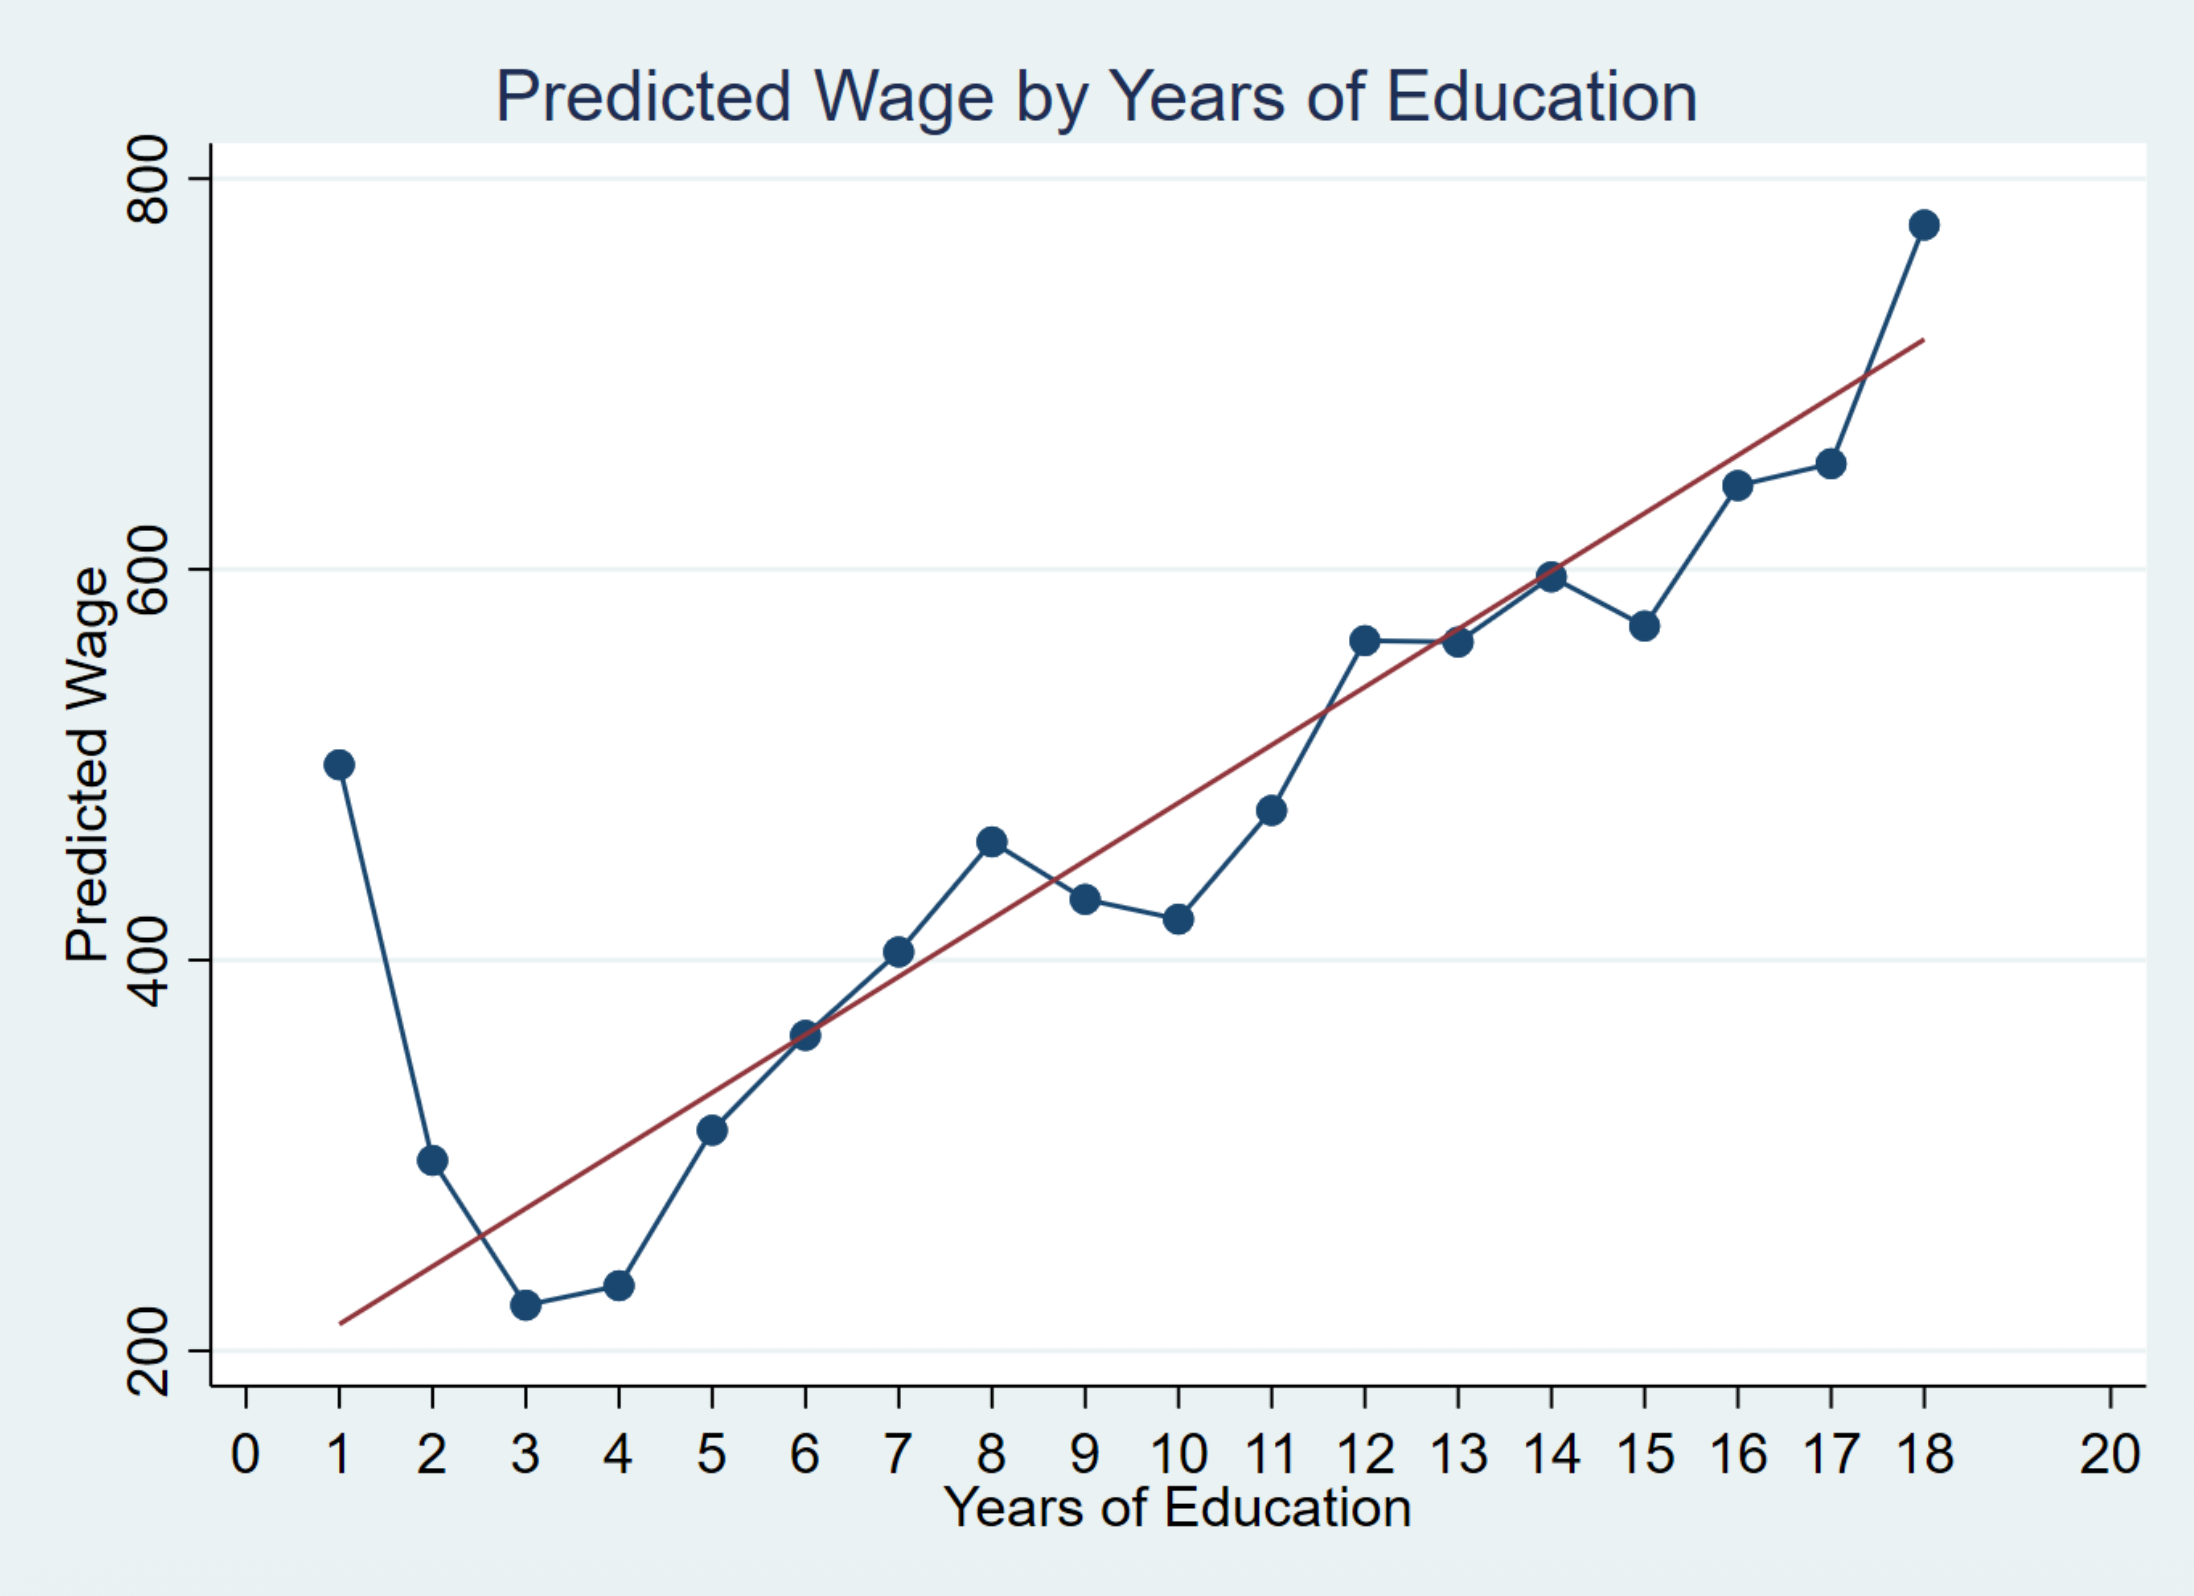
\includegraphics[width=0.78\textwidth]{images/1-22-1}
\end{figure}

There is a small sample problem for years of education less than 8. We trade off variance at this low end, getting a higher bias.

\begin{definition}[Best Linear Predictor]
	The best linear predictor of $y$ given $x$ is defined by
	\[
		\beta=\E\left[xx'\right]^{-1}\E\left[xy\right],
	\]
	where the FOC implies $\E\left[xy\right]=\E\left[xx'\right]\beta$. In order for these equations to have a unique solution, $\E\left[xx'\right]$ must be full rank/invertible. This is equivalent to there being no perfect multicollinearity in $x$; i.e., there is no $a\in \R^k\setminus \{0\}$ such that $x'a = 0$ with probability $1$.
\end{definition}

\section{OLS Estimation}

\begin{remark}	Given a sample $\{y_i,x_i\}_{i=1}^n$, we can apply the sample analogue principle\footnote{Now, $\theta(f)$ is defined as an $\argmin$ of an objective function. We find $\theta(\hat{f})$ now.} and solve the analogous in-sample problem:
	\[
		\min_{b\in\R^k}\frac{1}{n}\sum_{i=1}^n\left(y_i-x_i'b\right)^2
	\]
	to yield an estimator of $\beta$.\boxednote{The solution is $\hat{\beta} = (\frac{1}{n} \sum_i X_iX_i')^{-1} \frac{1}{n} \sum_i X_i Y_i$.} The first order conditions with respect to each $b_j$ imply that at the solution\boxednote{We think of a matrix of $x$ with the rows as observations $1:n$ and the columns as dimensions of $x$ from $1:k$. The first column will be $\vec 1$. Basically, we attach a $1$ to the meaningful characteristics of $x_i$ to get the intercept $\beta_0$ when multiplying by $X$. For example, if we want to consider predicting house price with number of bedrooms, a house would be represented by $(x_i;ly_i) = (1, \text{rooms}; \text{price})$. We want to allow the prediction line to not pass through the origin so the $\beta$s are interpretable as partial covariances.}:
	\[
		-2\cdot\frac{1}{n}\sum_{i=1}^n x_{ij}\left(y_i-x_i'\hat\beta\right)=0\quad\text{for all }1\le j\le k.
	\]

	Stacking these first order conditions gives
	\[
		\begin{pmatrix}
			\frac{1}{n}\sum_{i=1}^n x_{i1}(y_i-x_i'\hat\beta) \\
			\vdots                                            \\
			\frac{1}{n}\sum_{i=1}^n x_{ik}(y_i-x_i'\hat\beta)
		\end{pmatrix}
		=
		\frac{1}{n}\sum_{i=1}^n x_i(y_i-x_i'\hat\beta)=0.
	\]

	Adding $\left( \frac{1}{n} \sum_i x_i x_i' \right)\hat{\beta}$, we get that the FOCs imply
	\[
		\frac{1}{n}\sum_{i=1}^n x_iy_i=\left(\frac{1}{n}\sum_{i=1}^n x_ix_i'\right)\hat\beta.
	\]
	Provided $\frac{1}{n}\sum_{i=1}^n x_ix_i'$ is invertible, which occurs iff none of the columns $x_{\cdot j}$ are collinear, we obtain\boxednote{We can think of $(X_i,Y_i) \in \R^{k+1}$ so our estimator is an object in $\R^{k}$.}
	\[
		\hat\beta=\left(\frac{1}{n}\sum_{i=1}^n x_ix_i'\right)^{-1}\frac{1}{n}\sum_{i=1}^n x_iy_i.
	\]
\end{remark}

\begin{definition}[Fitted Values and Residuals]
	The $i$-th fitted value is:
	\[
		\hat y_i=x_i'\hat\beta.
	\]
	The $i$-th residual is
	\[
		\hat u_i=y_i-\hat y_i.
	\]
\end{definition}

\begin{remark}[FOC of OLS]
	The first order condition of the least squares minimization problem implies
	\[
		\sum_{i=1}^n x_i(y_i-x_i'\hat\beta)=\sum_{i=1}^n x_i\hat u_i=0.
	\]
	We can write this compactly as $X'\hat{u} = 0$.
\end{remark}

\begin{example}[Simple Linear Regression]
	Consider the simple linear model:
	\[
		y=\beta_0+\beta_1x_1+u,
	\]
	where now $x=(1,x_1)'$, and $\beta=(\beta_0,\beta_1)'$. Our earlier work implies\boxednote{Note that this expression for $\beta$ holds regardless of the dimension of $X$.}
	\[
		\beta=\E\left[xx'\right]^{-1}\E\left[xy\right].
	\]
	We have
	\begin{align*}
		\E\left[xx'\right]^{-1}
		&=\begin{pmatrix}
			1   & x_1   \\
			x_1 & x_1^2
		\end{pmatrix}^{-1}
		=\frac{1}{\E\left[x_1^2\right]-\E\left[x_1\right]^2}\begin{pmatrix}
			\E\left[x_1^2\right] & -x_1 \\
			-x_1                 & 1
		\end{pmatrix}, \\
		\E\left[xy\right]
		&=\begin{pmatrix}
			\E\left[y\right] \\
			\E\left[x_1y\right]
		\end{pmatrix}.
	\end{align*}
	It follows that\boxednote{\texthl{apparently this was done in the hw??}}
	\[
		\beta=\frac{1}{\operatorname{Var}(x_1)}\cdot\begin{pmatrix}
			\E\left[x_1^2\right] & -\E\left[x_1\right] \\
			-\E\left[x_1\right]  & 1
		\end{pmatrix}\begin{pmatrix}
			\E\left[y\right] \\
			\E\left[x_1y\right]
		\end{pmatrix}
		=\begin{pmatrix}
			\E\left[y\right]-\beta_1\E\left[x_1\right] \\
			\frac{\operatorname{Cov}(y,x_1)}{\operatorname{Var}(x_1)}
		\end{pmatrix}.
	\]
\end{example}

\begin{remark}[Slope Parameter and Correlation]
	Notice that
	\[
		\beta_1=\frac{\operatorname{Cov}(W,S)}{\operatorname{Var}(S)}=\sqrt{\frac{\operatorname{Var}(W)}{\operatorname{Var}(S)}}\cdot\operatorname{Corr}(W,S),
	\]
	so the slope coefficient is proportional to the correlation between wages and education (likely $>0$).

	Notice that increasing $\operatorname{Var}(W)$ stretches the scatter plot vertically (but leaves the correlation unchanged). The slope coefficient should increase in magnitude.

	Increasing $\operatorname{Var}(S)$ stretches the scatter plot horizontally (but leaves the correlation unchanged). The slope coefficient should decrease in magnitude.
\end{remark}

\begin{example}[Changing units of measurement]
	Suppose wages are now measured in cents per hour rather than dollars per hour. Let $\tilde W$ denote wages in cents:
	\[
		\tilde W=100W.
	\]
	Find the best linear predictor of $\tilde W$ given $S$, i.e. find $(\alpha_0,\alpha_1)$ such that\boxednote{\texthl{ why is including the condition on the expectation of $SU$, $U$ and finding the best linear predictor equivalent to the minimization problem without the error term?}}
	\[
		\tilde W=\alpha_0+\alpha_1S+U;\qquad \E\left[SU\right]=\E\left[U\right]=0.
	\]
	Find that
	\[
		\alpha_1=\frac{\operatorname{Cov}(\tilde W,S)}{\operatorname{Var}(S)}=\frac{100\operatorname{Cov}(W,S)}{\operatorname{Var}(S)}=100\beta_1,
	\]
	\[
		\alpha_0=\E\left[\tilde W\right]-\alpha_1\E\left[S\right]=100(\E\left[W\right]-\beta_1\E\left[S\right])=100\beta_0.
	\]
\end{example}

\begin{example}[Simple Linear Regression Estimation]
	Write the model for each individual $i=1,\ldots,n$ in the sample:
	\[
		y_i=\beta_0+\beta_1x_{i1}+u_i,
	\]
	and estimate the parameters using ordinary least squares:
	\[
		\hat\beta=\left(\frac{1}{n}\sum_{i=1}^n x_ix_i'\right)^{-1}\frac{1}{n}\sum_{i=1}^n x_iy_i
		=\begin{pmatrix}
			\bar y_n-\hat\beta_1\bar x_{1,n} \\
			\frac{\frac{1}{n}\sum_{i=1}^n x_{i1}y_i-\bar x_{1,n}\cdot\bar y_n}{\frac{1}{n}\sum_{i=1}^n x_{i1}^2-(\bar x_{1,n})^2}
		\end{pmatrix}.
	\]
\end{example}

\section{Matrix Notation and Projection}

\begin{remark}[Matrix Notation]
	First write the model for each observation $i=1,\ldots,n$:
	\[
		y_i=x_i'\beta+u_i.
	\]
	Stack the observations into matrices:
	\[
		\begin{pmatrix}
			y_1    \\
			y_2    \\
			\vdots \\
			y_n
		\end{pmatrix}
		=
		\underbrace{\begin{pmatrix}
			-x_1'- \\
			-x_2'- \\
			\vdots \\
			-x_n'-
		\end{pmatrix}}_{\text{design matrix}}
		\beta
		+
		\begin{pmatrix}
			u_1    \\
			u_2    \\
			\vdots \\
			u_n
		\end{pmatrix}.
	\]
	Therefore
	\[
		Y=X\beta+U,
	\]
	where the matrix $X$ is called the design matrix, with columns $X_1,\ldots,X_k\in\R^n$. If we have an intercept, then the first feature $X_1$ is a column of $1$s.

	The least squares minimization problem is
	\[
		\min_{b\in\R^k}\sum_{i=1}^n(y_i-x_i'b)^2\equiv\min_{b\in\R^k}(Y-Xb)'(Y-Xb) = \min_{B \in \R^k} \|Y - Xb\|^2
	\]
	because the sum of squares is just the inner product of $Y-Xb$ with itself.
	To see this, write \[
		\R^n \ni Y - Xb = \begin{bmatrix}
		y_1-x_1'b \\
		\vdots \\
		y_n - x_n'b
		\end{bmatrix} 
	,\] so \[
	\left( Y-Xb \right)'(Y-Xb) = \sum\limits_{i=1}^{n} \left( y_i - x_i'b \right)^2
	.\] Hence, we want to pick $b$ to minimize the distance from $Xb \in \operatorname{Span}(X)$ to $Y\in \R^n$ in the Euclidean norm. This is the point that is the orthogonal projection of $Y$ onto $\operatorname{Span}(X)$.

	We can expand the objective function as
	\[
		(Y-Xb)'(Y-Xb)=Y'Y-Y'Xb-b'X'Y+b'X'Xb=Y'Y-2Y'Xb+b'X'Xb,
	\]
	so the first order condition with respect to $b_j$ is
	\[
		-2\sum_{i=1}^n y_i\cdot x_{ij}+2\sum_{i=1}^n x_{ij}\cdot x_i'\hat\beta=0.
	\]
	Stack the first order conditions into a $k\times 1$ vector:
	\[
		-2\sum_{i=1}^n y_i\cdot x_i+2\left[\sum_{i=1}^n x_ix_i'\right]\hat\beta=0;\quad\text{or}\quad
		-2X'Y+2X'X\hat\beta=0.
	\]
	This yields $X'\left( Y- X\hat{\beta} \right) = 0$,\footnote{This says that every column of $X$ (row of $X'$) is orthogonal to the residual (row).} which is equivalent to (provided $X$ is full column rank):
	\[
		\hat\beta=(X'X)^{-1}X'Y.
	\]
\end{remark}

\begin{remark}	We have used the fact that
	\[
		\sum_{i=1}^n x_ix_i'=X'X,\qquad
		\sum_{i=1}^n y_ix_i=X'Y.
	\]
	To see why these identities hold, consider $X \in \R^{n\times k}$ and $X' \in \R^{k\times n}$, so \[
		X'X = \begin{bmatrix}
			\sum\limits_{i=1}^{n} x_{i_1}^2 & \sum\limits_{i=1}^{n} x_{i 1} x_{i 2} & \cdots \\
		\sum\limits_{i=1}^{n} x_{i 2}x_{i 1} & \sum\limits_{i=1}^{n} x_{i 2}^2 & \cdots \\
		\vdots & & \ddots
		\end{bmatrix} = \sum\limits_{i=1}^{n} X_i X_i'
	.\] Switching a transpose between matrices and vectors moves the transpose.

	The vector of fitted values is $\hat Y=X\hat\beta$, and the vector of residuals is $\hat U=Y-\hat Y$. The FOC of the least squares problem is equivalently written as $X'\hat U=0$. These are the normal equations.
\end{remark}

\begin{proposition}	$(X'X)^{-1}$ exists iff $X$ is full column rank.

	If $X$ is not full column rank, there exists $c\neq 0$ such that $Xc=0$, so $X'Xc=0$, implying $X'X$ is not invertible.

	If $X'X$ is not invertible, there exists $a\neq 0$ such that $X'Xa=0$, so $a'X'Xa=0$. But
	\[
		a'X'Xa=[Xa]'(Xa),
	\]
	which is a sum of squares which equals zero iff $Xa=0$. Since $a\neq 0$, $X$ is not full rank.

	In a simple linear regression, need there to be some variation in $\left( X_i \right)_{1:n}$ so it isn't collinear with the constant. Equivalently, need $\det(X'X)=(n-1)\cdot\widehat{\operatorname{Var}}(x)\neq 0$. When $X_i \in R^2$ with a column of $1$s, then we require that the 2nd column of $X$ is not identically some constant.
\end{proposition}

\begin{theorem}[Projection Theorem]
	Let $y\in\R^n$ and let $S$ be any nonempty subspace of $\R^n$ equipped with the dot product. There exists a unique point $\hat y$ such that $\|y-\hat y\|$ is minimized over $S$.\boxednote{Here, we are thinking of $S$ as a $k$-dimensional subspace of $\R^n$ --- the subset of $\R^n$ spanned by the columns of $X$.} A necessary and sufficient condition for $\hat y$ is that $\hat{y} \in S$ and $\hat y-y$ is orthogonal to every vector in $S$.

	By definition of $\hat\beta$, the vector $X\hat\beta$ is the closest (in the Euclidean norm) to $Y$ in the set of all vectors
	\[
		\{Xb:b\in\R^k\}=S(X),
	\]
	where $S(X)$ denotes the span of the columns of $X$. Given a vector $Y\in\R^n$ and a matrix $X\in\R^{n\times k}$, the projection of $Y$ onto $S(X)$ is the vector\footnote{We previously found $v^* = X\hat{\beta}$.}
	\[
		v^*\in\argmin_{v\in S(X)}\|Y-v\|^2.	
	\]

	While the coefficients $\hat{\beta}$ may not be unique (if $X$ is not full column rank), this theorem guarantees that $X\hat{\beta}$ is unique. 
\end{theorem}

\begin{example}	We can draw the following to provide intuition. Consider $n=2$, $k=2$, and a model with no intercept, so $y_i = \beta x_i + u_i$. Suppose $X = \begin{pmatrix}
	x_1 \\
	x_2
	\end{pmatrix} = \begin{pmatrix}
	1 \\
	0
	\end{pmatrix} $ and $Y = \begin{pmatrix}
	3 \\
	3
	\end{pmatrix} $.

	In this case, $S(X) = \{c \begin{pmatrix}
	1 \\
	0
	\end{pmatrix} : c\in \R\}$, so \[\hat{Y} = P_X Y = \begin{pmatrix}
	3 \\
	0
	\end{pmatrix}, \quad\hat{U} = \begin{pmatrix}
	0 \\
	3
\end{pmatrix}.\]

	We note that $P_X Y$ is the closest point to $Y$ in $S(X)$, while $\hat{U}$ is orthogonal to $S(X)$.
\end{example}


\begin{remark}	Restricting the minimizer to vectors in $S(X)$, the necessary and sufficient condition for the minimizer is
	\[
		x'(Y-\hat Y)=0
	\]
	for all $x\in S(X)$. Since the columns of $X$ are a basis of $S(X)$, this condition is equivalent to
	\[
		X'(Y-\hat Y)=0.
	\]
	$\hat Y\in S(X)$ means $\hat Y=Xb$ for some $b\in\R^k$. Thus
	\[
		X'Y=X'Xb\implies b=(X'X)^{-1}X'Y\implies\hat Y=X(X'X)^{-1}X'Y.
	\]
	That is, the projection of $Y$ onto $S(X)$ is given by $\hat Y=P_XY$, where $P_X$ is the projection matrix defined below.
\end{remark}

\begin{definition}[Projection Matrix]
	Since $X\hat\beta=X(X'X)^{-1}X'Y$, we call $P_X=X(X'X)^{-1}X'$ the projection matrix (it projects $Y$).

	The projection matrix is symmetric:
	\[
		P_X'=[X(X'X)^{-1}X']'=X[(X'X)^{-1}]'=X[(X'X)']^{-1}X'=P_X.
	\]
\end{definition}

\begin{remark}	$P_X$ is also idempotent (meaning $P_X\cdot P_X=P_X$), since:
	\[
		P_XP_X=X(X'X)^{-1}X'X(X'X)^{-1}X'=X(X'X)^{-1}X'=P_X,
	\]
	which reflects the fact that after a vector has been projected on to the span of the columns of $X$, it does not change as a result of the second projection. This is because the projected vector is already a linear combination of the columns of $X$.
\end{remark}

\begin{definition}[Residual Maker Matrix]
	The residual of the projection of $Y$ onto the columns of $X$ is
	\[
		Y-\hat Y=Y-P_XY=(I_n-X(X'X)^{-1}X')Y.
	\]
	Therefore, the matrix $M_X:=I_n-X(X'X)^{-1}X' = I_n - P_X$ is called the residual maker.

	$M_XY$ is the residual of the projection of $Y$ onto the space spanned by the columns of $X$.
\end{definition}

\begin{proposition}[Properties of Residual Maker]
	$M_X$ projects a vector onto the $n-k$ dimensional vector space orthogonal to the column space of $X$. This is called the orthogonal complement of $S(X)$.

	The residual of the projection $M_X y$ is $y - M_X y = P_X y \in S(X) \perp OC(S(X))$.

	Some properties:
	\begin{itemize}
		\item $P_XM_X=M_XP_X=0$, since $P_X(I-P_X)=P_X-P_XP_X=0$.
		\item $P_XX=X(X'X)^{-1}X'X=X$: Projecting $X$ onto its own span does nothing.
		\item $M_XX=X-P_XX=0$: Residual of projecting $X$ onto its own span is $0$.
		\item For any vector $y$, $y=P_Xy+M_Xy=\hat y+\hat u$.
	\end{itemize}
\end{proposition}

\section{$R^2$ and Goodness of Fit}

\begin{definition}[$R^2$]
	\begin{itemize}
		\item $\sum_{i=1}^n(y_i-\bar y)^2:=\text{TSS}$ is called the total sum of squares.
		\item $\sum_{i=1}^n(y_i-x_i'\hat\beta)^2:=\text{SSR}$ is the sum of squared residuals.
		\item $\sum_{i=1}^n(\hat y_i-\bar y)^2:=\text{ESS}$ is the explained sum of squares.
	\end{itemize}
	The coefficient of determination ($R^2$) is given by
	\[
		R^2=\frac{\text{ESS}}{\text{TSS}}.
	\]
\end{definition}

\begin{remark}	Immediately, we see that $SSR \le TSS$ because the $SSR$ is the residuals from letting our line of fit to have a free intercept and slope, while $TSS$ fixes a slope of $0$.
	$R^2$ measures how well OLS estimation of a linear model which includes a constant as a regressor fits a given dataset relative to a model only containing a constant. In other words, we are comparing two models:
	\begin{enumerate}[label=(\roman*)]
		\item $y = \beta_0 + u$, which implies $\hat{\beta}0^{OLS} = \overline{y}$
		\item $y = \beta_0 + \beta_1 x + \epsilon$,
	\end{enumerate}
	and seeing what fraction the SSR of the second model is of the SSR of the first model.
	

	We have:
	\[
		R^2=\frac{\text{ESS}}{\text{TSS}}=\frac{\sum_{i=1}^n(\hat y_i-\bar y_n)^2}{\sum_{i=1}^n(y_i-\bar y_n)^2}=1-\frac{\sum_{i=1}^n(y_i-x_i'\hat\beta)^2}{\sum_{i=1}^n(y_i-\bar y_n)^2},
	\]
	where the third equality follows from $SSR + ESS = TSS$ (shown later).

	The second and third equalities imply $0\le R^2\le 1$.

	$R^2=1$ iff $\text{SSR}=0$, which means $\hat U=0$.

	$R^2=0$ iff $\text{SSR}=\text{TSS}$, which implies all $y_i$ are identical and $\hat\beta=(\bar y,0,\ldots,0)$ provided $X$ is full column rank. In this case the model fits the data no better than a constant would; knowing $x$ does not help us predict $y$.
\end{remark}

\begin{proof} (Decomposition of $R^2$)
	Let $P_c=\mathbf{1}(\mathbf{1}'\mathbf{1})^{-1}\mathbf{1}'=\frac{1}{n}\mathbf{1}\mathbf{1}'$ be the projection matrix onto the span of the column vector of ones in $\R^n$. Then $P_cY=\frac{1}{n}\mathbf{1}\mathbf{1}'Y=\bar y_n\mathbf{1}$, so:
	\begin{align*}
		\text{TSS}&=\|Y-P_cY\|^2=\|M_cY\|^2 \\
		\text{ESS}&=\|P_XY-P_cY\|^2=\|P_XY-P_XP_cY\|^2=\|P_XM_cY\|^2 \\
		\text{SSR}&=\|Y-P_XY\|^2=\|M_XY\|^2=\|M_XM_cY\|^2.
	\end{align*}\boxednote{We see that \begin{align*}
		M_X M_c Y &= M_X Y - M_X P_c Y \\
		           &= M_X Y,
	\end{align*}since $P_c Y\in S(X)$ means $M_X P_c Y=0$.}

	Finally, since $P_XM_cY \in S(X)$ and $M_XM_cY \in OC(S(X))$ are orthogonal:
	\[
		\|M_XM_cY\|^2+\|P_XM_cY\|^2=\|M_XM_cY+P_XM_cY\|^2=\|M_cY\|^2,
	\]
	so $\text{ESS}+\text{SSR}=\text{TSS}$. This shows that
	\[
		R^2=\frac{\text{ESS}}{\text{TSS}}=1-\frac{\text{SSR}}{\text{TSS}}.
	\]
\end{proof}

\begin{remark}	High $R^2$ does not mean the linear model is ``correct'' in the sense that it provides a causal explanation of the relationship between $x$ and $y$.

	On the other hand, low $R^2$ does not preclude a causal relationship between $x$ and $y$ in a linear model.

	$R^2$ is an estimator of the population $R^2$, defined by
	\[
		R^2_{\text{pop}}=1-\frac{\operatorname{Var}(u)}{\operatorname{Var}(y)},
	\]
	since $\text{SSR}/n$ is an estimate of $\operatorname{Var}(u)$ and $\text{TSS}/n$ is an estimate of $\operatorname{Var}(y)$.

	Decomposing variance in $y$ as
	\[
		\operatorname{Var}(y):=\E\left[\operatorname{Var}(y\mid x)\right]+\operatorname{Var}(\E\left[y\mid x\right]).
	,\]
	the first term represents the unexplained variation in $y$\footnote{Since $\operatorname{Var}\left(y \mid x\right) = \E\left[\left( y - \E\left[y\mid x\right]  \right)^2\right]$ is the square of expected residual against the best linear predictor.}, while the second term represents variation in $y$ that is explained by the model.
\end{remark}

\begin{remark}	Note that SSR always weakly decreases when a regressor is added to the model.

	Suppose we estimate the intercept and slope parameters in the following models by OLS:
	\[
		A:y_i=\alpha_0+\alpha_1x_{i1}+u_i;\qquad
		B:y_i=\beta_0+\beta_1x_{i1}+\beta_2x_{i2}+v_i.
	\]
	Let $\text{SSR}_A$ be the SSR resulting from OLS estimation of $A$, and $\text{SSR}_B$ be the SSR resulting from OLS estimation of $B$.

	We have
	\[
		\text{SSR}_A=\min_{a_0,a_1}\sum_{i=1}^n(y_i-a_0-a_1x_{i1})^2=\sum_{i=1}^n(y_i-\hat\alpha_0-\hat\alpha_1x_{i1})^2;
	\]
	\[
		\text{SSR}_B=\min_{b_0,b_1,b_2}\sum_{i=1}^n(y_i-b_0-b_1x_{i1}-b_2x_{i2})^2=\sum_{i=1}^n(y_i-\hat\beta_0-\hat\beta_1x_{i1}-\hat\beta_2x_{i2})^2.
	\]

	$\text{SSR}_B\le\text{SSR}_A$: after finding $(\hat\alpha_0,\hat\alpha_1)$, setting $(b_0,b_1,b_2)=(\hat\alpha_0,\hat\alpha_1,0)$ is always feasible. In general, the optimal $b_2\ne0$, so adding $x_2$ strictly reduces SSR.

	This also means $R^2$ increases when adding regressors, because
	\[
		R^2_A=1-\frac{\text{SSR}_A}{\text{TSS}}\le 1-\frac{\text{SSR}_B}{\text{TSS}}=R^2_B.
	\]
\end{remark}

\begin{definition}[Adjusted $R^2$]
	Adjusted $R^2$ penalizes additional regressors, and is defined by
	\[
		\bar R^2=1-\frac{n-1}{n-k-1}\frac{\text{SSR}}{\text{TSS}}=1-\frac{n-1}{n-k-1}(1-R^2)\le R^2
	,\]
	where $k$ is the number of regressors (excluding the intercept) and $n$ is the sample size.
\end{definition}

\section{Finite Sample Properties of OLS}

Economists don't care too much about $R^2$ because it's a measure of prediction accuracy, not causality.

\begin{remark}[Gauss Markov Assumptions]
	We will work with the following assumptions to provide an ideal setting for linear regression, then derive the expectation and variance of OLS estimators:
	\begin{itemize}
		\item MLR.1: The model under consideration is
		      \[y=\beta_0+\beta_1x_1+\cdots+\beta_kx_k+u\equiv x'\beta+u.\]
		      \boxednote{By itself, MLR.1 imposes no restriction on $x$ because we can put $u = y - x'\beta$ and always represent $y$ in this way.}
		\item MLR.2: We observe an iid sample of $\{y_i,x_i\}_{i=1}^n$.
		\item MLR.3: There is no perfect collinearity in the sample (so $\left( X'X \right)^{-1}$ exists with probability $1$ and a unique $\hat\beta$ exists).
		\item MLR.4: $\E\left[u\mid x\right]=0$.\footnote{Hence, $\E\left[y \mid x\right] $ is a linear function of $x$.}
		\item MLR.5: (Homoskedasticity) $\operatorname{Var}(y\mid x)=\sigma^2$.\footnote{There is generally no good reason to believe in homoskedasticity. Correcting for heteroskedasticity would weight sample points where the error variance is lower, since these points give more information on the relationship between $y$ and $x$. This leads to generalized OLS, which is not used often because a heteroskedasticity correction is difficult (the standard deviation of the error as a function of $x$ is not known).}
	\end{itemize}
	MLR stands for multiple linear regression.
\end{remark}

\begin{proposition}	Suppose MLR.1--MLR.4 hold. By $\E\left[u\mid x\right] =0$ and since $(u_i,x_i)$ is independent of $x_j$ for $j\neq i$, we obtain for each $i$:
	\[
		0=\E\left[u_i\mid x_i\right]=\E\left[u_i\mid x_1,\ldots,x_n\right].
	\]
	This is equivalently written as
	\[
		\E\left[U\mid X\right]=0.
	\]
	This is in turn equivalent to
	\[
		\E\left[Y\mid X\right]=X\beta.
	\]
\end{proposition}
\begin{proof}
	(Bias.) It follows that
	\begin{align*}
		\E\left[\hat\beta\mid X\right]
		&=\E\left[(X'X)^{-1}X'Y\mid X\right]=(X'X)^{-1}X'\E\left[Y\mid X\right] \\
		&=(X'X)^{-1}X'X\beta=\beta.
	\end{align*}
	By the Law of Iterated Expectation:
	\[
		\E\left[\hat\beta\right]=\E\left[\E\left[\hat\beta\mid X\right]\right]=\beta,
	\]
	so $\hat\beta$ is unbiased.

	(Variance.) Suppose in addition that $\operatorname{Var}(u_i\mid x_i)=\sigma^2$. (MLR.5)

	Since the error variance does not depend on the value of $x_i$, it is called homoskedastic. If the error variance depends on $x_i$, $u_i$ is heteroskedastic and MLR.5 fails.

	Under homoskedasticity,
	\[
		\operatorname{Var}(U\mid X)=\sigma^2I_n.
	\]
	To see this, note that the $(i,j)$ entry is given by
	\[
		\operatorname{Var}(U\mid X)_{i,j}=\E\left[UU'\mid X\right]_{i,j}=\E\left[u_iu_j\mid X\right]=
		\begin{cases}
			\E\left[u_i^2\mid x_i\right]      & i=j      \\
			\E\left[u_iu_j\mid x_i,x_j\right] & i\neq j.
		\end{cases}
	\]

	We have $\E\left[u_i^2\mid x_i\right]=\sigma^2$ because
	\[
		\E\left[u_i^2\mid x_i\right]-\underbrace{(\E\left[u_i\mid x_i\right])^2}_{=0}=\operatorname{Var}(u_i\mid x_i)=\sigma^2.
	\]
	We also have that for $i\ne j$,
	\[
		\E\left[u_iu_j\mid x_i,x_j\right]=\E\left[u_i\E\left[u_j\mid u_i,x_i,x_j\right]\mid x_i,x_j\right]=\E\left[u_i\E\left[u_j\mid x_j\right]\mid x_i,x_j\right]=0.
	\] The off diagonal elements are $0$ because of MLR.2,\footnote{MK: and because of MLR.4, I think.} \emph{not} because of MLR.5.

	Under heteroskedasticity, the off diagonal elements are still $0$ but\[\E[u_i^2\mid x_i]=f(x_i),\]so
	\[
		\operatorname{Var}(U\mid X)=
		\begin{pmatrix}
			f(x_1) & 0      & 0      & 0      \\
			0      & f(x_2) & 0      & 0      \\
			0      & 0      & \ddots & 0      \\
			0      & 0      & 0      & f(x_n)
		\end{pmatrix} =: \Omega
		.\]

	We now conclude that (*)
	\[
		\operatorname{Var}(\hat\beta\mid X)=\operatorname{Var}(\beta+(X'X)^{-1}X'U\mid X)=(X'X)^{-1}X'\Omega X(X'X)^{-1}.
	\]
	Under homoskedasticity, $\Omega=\sigma^2I_n$, and so the variance becomes
	\[
		\operatorname{Var}(\hat\beta\mid X)=\sigma^2(X'X)^{-1}X'I_nX(X'X)^{-1}=\sigma^2(X'X)^{-1}.
	\]

	(*) follows from $\hat{\beta} = \beta + \left( \underbrace{\left( X'X \right)^{-1}X'}_{A(X)} U \mid X \right)$, so \[
		\operatorname{Var}\left(\left( \hat{\beta} \mid X \right)\right)= A(X) \operatorname{Var}\left(U \mid X\right) A(X)' = \sigma^2 \left( X'X \right)^{-1}
	,\] where the last equality follows from MLR.5.
\end{proof}

\begin{theorem}[Gauss-Markov Theorem]
	Under MLR.1--5, the OLS estimator is the ``best linear unbiased estimator'', which means it has the ``smallest'' variance in the class of linear estimators that are also unbiased conditional on $X$. This result is known as the Gauss-Markov Theorem.

	Our goal is to show that
	\[
		\operatorname{Var}(\hat\beta\mid X)=\sigma^2(X'X)^{-1}
	\]
	is ``smaller'' than the conditional variance of any other estimator $\tilde\beta=A(X)Y$ which also satisfies $\E\left[\tilde\beta\mid X\right]=\beta$. Precisely: $\operatorname{Var}(\tilde\beta\mid X)-\operatorname{Var}(\hat\beta\mid X)=D$ is a positive-semidefinite matrix.
\end{theorem}

\begin{remark}	In particular, let $r$ be a $k\times 1$ vector, and let $r'\beta$ denote a linear combination of the $\beta_j$. The Gauss-Markov theorem implies that $r'\hat\beta$ is the Best Linear Unbiased Estimator of $r'\beta$, since
	\[
		\operatorname{Var}(r'\tilde\beta\mid X)-\operatorname{Var}(r'\hat\beta\mid X)=r'\operatorname{Var}(\tilde\beta\mid X)r-r'\operatorname{Var}(\hat\beta\mid X)r=r'Dr\ge 0.
	\]
	For example, if $r=(0,0\ldots,0,\underbrace{1}_{\text{$j$-th position}},0,\ldots,0)$, then $r'\hat\beta=\hat\beta_j$, and so $\operatorname{Var}(\hat\beta_j\mid X)\le\operatorname{Var}(\tilde\beta_j\mid X)$.
\end{remark}

\begin{proof}(Gauss-Markov Theorem)
	Now consider any other linear unbiased (conditional on $X$) estimator of $\beta$ defined by \[
		\tilde{\beta} = A(X) Y
	.\] Recall that $\hat{\beta} = A(X) = \left( X'X \right)^{-1}X'$. Note that 
	\begin{align*}
		\E\left[\tilde{\beta} \mid X\right]  &= \E\left[A(X) Y \mid X\right]  \\
		&= A(X) \E\left[Y \mid X\right]  \\
		&= A(X) X \beta
	,\end{align*}
	which must be equal to $\beta$ for any $\beta \in \R^k$ if $\tilde{\beta}$ is unbiased. In this case, for any $\beta \in \R^k$, \[
		\left( A(X) X - I_k \right)\beta = 0
	,\] so \[
		A(X)X = I_k
	.\] 
	Therefore, if we require $\hat{\beta}$ to be unbiased, we require $A(X) X = I_k$. Note that $A(X)$ as defined in OLS satisfies this.

	From now on, write $A := A\left( X \right)$.

	Next, we compute the variance of $\tilde{\beta} = AY$ conditional on $X$:
	\[
		\operatorname{Var}\left(\tilde{\beta} \mid X\right) = \operatorname{Var}(AY\mid X)=A\operatorname{Var}(Y\mid X)A'=A\operatorname{Var}(U\mid X)A'=\sigma^2AA'.
	\]
	If $A=(X'X)^{-1}X'$, we obtain the OLS estimator, with variance $\sigma^2(X'X)^{-1}$.

	We really want to show that $\operatorname{Var}\left(\tilde{\beta}\mid X\right) \ge \operatorname{Var}\left(\hat{\beta} \mid X\right)$. But how should we define an ordering of matrices? One way is to say that the first matrix is larger if the difference of the first minus the second is positive semidefinite. This is because taking a linear combination of the $\hat{\beta}$ estimate's components with a vector $r$ multiplies the variance by $r$ and $r'$ on either side, respectively.

	Define $C = A - (X'X)^{-1}X'$, so that $A = C + (X'X)^{-1}X'$. Note that the unbiasedness constraint $AX = I_k$ gives
	\[
		CX = AX - (X'X)^{-1}X'X = I_k - I_k = 0.
	\]
	Expanding $AA'$:
	\begin{align*}
		AA' &= \Bigl(C + (X'X)^{-1}X'\Bigr)\Bigl(C + (X'X)^{-1}X'\Bigr)' \\
		    &= CC' + \underbrace{CX}_{=\,0}(X'X)^{-1} + (X'X)^{-1}\underbrace{(CX)'}_{=\,0} + (X'X)^{-1}X'X(X'X)^{-1} \\
		    &= CC' + (X'X)^{-1}.
	\end{align*}
	Therefore,
	\begin{align*}
		\operatorname{Var}\left(\tilde{\beta} \mid X\right) - \operatorname{Var}\left(\hat{\beta} \mid X\right)
			&= \sigma^2 AA' - \sigma^2(X'X)^{-1} \\
			&= \sigma^2\bigl[CC' + (X'X)^{-1}\bigr] - \sigma^2(X'X)^{-1} \\
			&= \sigma^2 CC'.
	\end{align*}
	Because $CC'$ is always positive semidefinite, we are done.

\end{proof}

\begin{remark}[Why positive semidefiniteness?]
	In particular,
	\begin{align*}
		\operatorname{Var}\left(\left( r' \hat{\beta} \mid X \right)\right) - \operatorname{Var}\left( r' \hat{\beta} \mid X\right) &=  r' \operatorname{Var}\left(\tilde{\beta} \mid X\right)r - r' \operatorname{Var}\left(\hat{\beta} \mid X\right)r \\
		&= r' \left[ \operatorname{Var}\left(\tilde{\beta }\mid X\right) - \operatorname{Var}\left(\hat{\beta} \mid X\right) \right]r \\
		&= \sigma^2 r' C C' r \ge 0
	,\end{align*}
	where the inequality follows from positive semidefiniteness of $C C'$. Therefore $r' \hat{\beta}$ is at least as efficient as $r' \tilde{\beta}$ for estimate $r' \beta$.
	In particular, \[
		\operatorname{Var}\left(\hat{\beta}_j \mid X\right) \le \operatorname{Var}\left( \left( \tilde{\beta}_j \mid X \right)\right)
	\] for any $j$. The OLS estimator $\hat{\beta}$ is efficient in the sense that componentwise, it achieves the lowest variance of an unbiased linear estimator of the conditional mean.\footnote{In fact, OLS is the best unbiased estimator (not restricting to just linear estimators). But doubly in fact, the only unbiased estimators are linear.}
\end{remark}


% Week 4 Slides
\section{Large Sample Properties of OLS}

\begin{assumption}	Now drop the assumptions that $\E\left[u_i \mid x_i\right] = 0$\footnote{i.e. that the relationship between $y$ and $x$ is linear.} and $\operatorname{Var}(u_i \mid x_i) = \sigma^2$ but assume we have an iid sample $\{y_i, x_i\}_{i=1}^n$.
	
	The model is \[
		y = x'\beta + u
	.\] 
	
	Suppose that $\E\left[ux\right] = 0$ and that $\E\left[xx'\right] $ is invertible. Note that $\frac{1}{n} \sum_{i=1}^{n} x_i x_i'$ may not be invertible under these assumptions (which was MLR.3), but it is invertible with probability approaching one because $\E\left[xx'\right] ^{-1}$ exists.
	
	In other words, the population condition that $\E\left[x x'\right]^{-1}$ existing is stronger (as in implies the sample condition) than the sample condition of $\frac{1}{n}\sum_{i=1}^{n} x_i x_i'$ being invertible.\boxednote{This is because if $\E\left[x x'\right] ^{-1}$ exists, the determinant of $\E\left[x x'\right] $ as a continuous function of $x$ is nonzero; convergence in probability gives a neighborhood of invertible matrices for which the determinant is nonzero. By the WLLN/convergence in probability, $\frac{1}{n}\sum x_i x_i'$ is eventually within this ball a.s.}
\end{assumption}

\begin{proposition}[Consistency]
	Under these weaker assumptions, the OLS estimator is consistent.
\end{proposition}
\begin{proof}
	First, note that \[
		\frac{1}{n} \sum_{i=1}^{n} x_i x_i' \xrightarrow{p} \E\left[xx'\right] ; \quad \frac{1}{n} \sum_{i=1}^{n} x_i y_i \xrightarrow{p} \E\left[xy\right] 
	.\] 
	by the law of large numbers, because $\{x_i x_i'\}_{i \ge 1}$ is an iid sequence of random matrices with expectation $\E\left[xx'\right] $, and $\{x_i y_i\}_{i \ge 1}$ is an iid sequence of random vectors with expectation $\E\left[xy\right] $.

	Marginal convergence in probability implies joint convergence in probability: \[
		\left( \frac{1}{n} \sum_{i=1}^{n} x_i x_i', \frac{1}{n} \sum_{i=1}^{n} x_i y_i \right) \xrightarrow{p} \left( \E\left[xx'\right] , \E\left[xy\right]  \right) 
	.\] 
	
	Now let $g(x,y) = x^{-1}y$, where $x^{-1}$ denotes a matrix inverse. $g$ is continuous if $x$ is invertible (matrix version of $x \ne 0$).
	
	It therefore follows by the continuous mapping theorem that \[
		\left( \frac{1}{n} \sum_{i=1}^{n} x_i x_i' \right)^{-1} \frac{1}{n} \sum_{i=1}^{n} x_i y_i \xrightarrow{p} \E\left[xx'\right] ^{-1} \E\left[xy\right] = \beta + \E\left[xx'\right] ^{-1} \E\left[xu\right] = \beta
	\] by plugging in $y = x' \beta + u$. 
\end{proof}

\begin{proposition}[Asymptotic Normality of OLS]
	Assume $\operatorname{Var}(xu)$ exists also. Then because $\E\left[xu\right] = 0 \implies \left( \E\left[xu\right]  \right)^2 = 0$, \[
		\operatorname{Var}(xu) = \E\left[xu(xu)'\right] = \E\left[u^2 xx'\right] 
	.\] 
	
	We have \[
		\sqrt{n} \left( \hat{\beta}_n - \beta \right) \xrightarrow{d} N(0, \Sigma)
	,\] where $\Sigma = \E\left[xx'\right] ^{-1} \operatorname{Var}(xu) \E\left[xx'\right] ^{-1}$.
\end{proposition}

\begin{proof}
	First note that \[
		\sqrt{n} \left( \hat{\beta}_n - \beta \right) = \left( \frac{1}{n} \sum_{i=1}^{n} x_i x_i' \right)^{-1} \frac{1}{\sqrt{n}} \sum_{i=1}^{n} x_i u_i
	.\] 

	Since the sequence of vectors $\left\{ (y_i, x_i')' \right\}_{i \ge 1}$ is iid, the sequence $\{x_i (y_i - x_i' \beta)\}_{i \ge 1}$ is iid. Therefore, the CLT implies:\boxednote{CLT applies:\begin{align*}\tfrac{1}{\sqrt{n}}\sum_i (X_i-\mu)&=\sqrt{n}(\bar X_n-\mu).\end{align*}} \[
		\frac{1}{\sqrt{n}} \sum_{i=1}^{n} x_i u_i \xrightarrow{d} N(0, \operatorname{Var}(xu))
	.\] 
	
	Applying Slutsky's Theorem gives \[
		\left( \frac{1}{n} \sum_{i=1}^{n} x_i x_i' \right)^{-1} \frac{1}{\sqrt{n}} \sum_{i=1}^{n} x_i u_i \xrightarrow{d} N(0, \Sigma)
	,\] as desired.
\end{proof}

\section{Estimation of $\Sigma$}

Deriving asymptotic normality of $\hat{\beta}$ will enable us to conduct hypothesis tests about the unknown parameter $\beta$.

Since we do not know $\Sigma$, we must construct a consistent estimator of it to yield an asymptotic distribution whose quantiles are known so we may conduct tests.

For the time being (the next two propositions), suppose MLR.4 and MLR.5 hold, so we have an easy case in which $\E\left[u \mid x\right] = 0$ and $\operatorname{Var}(u \mid x) = \sigma^2$. Then \[
	\operatorname{Var}(xu) = \E\left[u^2 xx'\right] = \E\left[\E\left[u^2 \mid x\right] xx'\right] = \E\left[\operatorname{Var}\left(u \mid x\right) x x'\right] = \sigma^2 \E\left[xx'\right] 
.\] 

It follows that \[
	\Sigma =  \E\left[x x'\right] ^{-1} \sigma^2  \E\left[x x'\right]  \E\left[x x'\right] ^{-1} = \sigma^2 \E\left[xx'\right] ^{-1}
.\] 


\begin{proposition}[$\hat{\sigma}^2$ is consistent]
	A natural estimator of $\E\left[xx'\right] ^{-1}$ is $\left( \frac{1}{n} \sum_{i=1}^{n} x_i x_i' \right)^{-1}$.\boxednote{The degree of freedom correction $k$ is the number of $\beta_j$s we are estimating. It is the width of the design matrix. Note that the adjusted $R^2$ does not count the intercept in its $k$, but when $k$ is the df correction, it is just always the number of $\beta$s to be estimated.}
	
	It remains to find a consistent estimator of $\sigma^2$. We use \[
		\hat{\sigma}^2 = \frac{1}{n-k} \sum_{i=1}^{n} \hat{u}_i^2 = \frac{\text{SSR}}{n-k}
	.\] 
	
	Next, note that $\hat{U} = M_X Y = M_X (X\beta + U) = M_X U$, so\footnote{The third equality follows from symmetry and idempotency of $M_X$.} \[
		\text{SSR} = \|M_X U\|^2 = U' M_X' M_X U = U' M_X U = U'U - U' P_X U
	.\] 
	Therefore, \[
		\begin{aligned}
			\hat{\sigma}^2
			&= \frac{\operatorname{SSR}}{n-k}
			= \frac{\operatorname{SSR}}{n}\frac{n}{n-k} \\
			&= \frac{n}{n-k} \left( \frac{1}{n} \sum_{i=1}^{n} u_i^2 - \left( \frac{1}{n} \sum_{i=1}^{n} u_i x_i' \right) \left( \frac{1}{n} \sum_{i=1}^{n} x_i x_i' \right)^{-1} \left( \frac{1}{n} \sum_{i=1}^{n} x_i u_i \right) \right) \\
			&\xrightarrow{p} \sigma^2 - 0 \cdot \E\left[xx'\right]^{-1} \cdot 0
			= \sigma^2
		\end{aligned}
	,\] by the continuous mapping theorem.
	
	Another application of the continuous mapping theorem implies that a consistent estimator of $\Sigma$ is given by \[
		\hat{\Sigma} = \hat{\sigma}^2 \left( \frac{1}{n} \sum_{i=1}^{n} x_i x_i' \right)^{-1} \xrightarrow{p} \sigma^2 \E\left[x x'\right]^{-1} = \Sigma
	.\] 
\end{proposition}

\begin{proposition}[$\hat{\sigma}^2$ is unbiased]
	We now show the degrees of freedom correction $n-k$ yields an unbiased estimate of $\sigma^2$. To see this, note that \[
		(n-k) \hat{\sigma}^2 = \text{SSR}
	,\] and
	\[
		\begin{aligned}
			\E\left[\text{SSR} \mid X\right]
			&= \E\left[U'U \mid X\right] - \E\left[U' P_X U \mid X\right] \\
			&= \sum_{i=1}^{n} \E\left[u_i^2 \mid X\right] - \E\left[U' P_X U \mid X\right] \\
			&= n\sigma^2 - \E\left[U' P_X U \mid X\right]
		\end{aligned}
	.\]
	We want to remove $P_X$ from the expectation, but it is in the middle of the product.

	Since expectations can be exchanged with summations, for a random matrix $A$: \[
		\E\left[\operatorname{tr}(A)\right] = \operatorname{tr}(\E\left[A\right] )
	.\] 
	
	The trace has a special property called invariance under cyclic permutations.
	
	For our purposes, this means that for any matrices $A, B$ such that $AB$ and $BA$ are well defined: \[
		\operatorname{tr}(AB) = \operatorname{tr}(BA)
	.\] 
	Since $U' P_X U$ is a scalar, it equals its trace, so \begin{align*}
		\E\left[U' P_X U \mid X\right] &= \E\left[\operatorname{tr}(U' P_X U) \mid X\right] \\ &= \E\left[\operatorname{tr}(P_X U U') \mid X\right] \\
									   &= \operatorname{tr}\left( P_X \E\left[UU' \mid X\right]  \right) \\
									   &= \operatorname{tr}(P_X \sigma^2 I_n) \\ &= \sigma^2 \operatorname{tr}\left( X(X'X)^{-1}X' \right)  \\ &= \sigma^2 \operatorname{tr}\left( X'X (X'X)^{-1} \right) \\ &= \sigma^2 \operatorname{tr}(I_k) \\ &= k\sigma^2
	.\end{align*} 
	
	This implies $\E\left[\text{SSR} \mid X\right] = n\sigma^2 - k\sigma^2 = (n-k)\sigma^2$, so $ \hat{\sigma}^2 = \frac{\E\left[\operatorname{SSR}\mid X\right] }{n-k}$ is an unbiased estimator of $\sigma^2$.
\end{proposition}

\begin{remark}
	If we do not assume $\E\left[u \mid x\right] = 0$ and $\operatorname{Var}(u \mid x) = \sigma^2$, $\Sigma$ does not simplify, and we use \[
		\hat{\Sigma} = \left( \frac{1}{n} \sum_{i=1}^{n} x_i x_i' \right)^{-1} \left( \frac{1}{n} \sum_{i=1}^{n} \hat{u}_i^2 x_i x_i' \right) \left( \frac{1}{n} \sum_{i=1}^{n} x_i x_i' \right)^{-1}
	.\] 
	
	Note that this is identical to $n \cdot (X'X)^{-1} X' \hat{\Omega} X (X'X)^{-1}$, where \[
		\hat{\Omega} = 
		\begin{pmatrix}
			\hat{u}_1^2 & 0 & 0 & 0 \\
			0 & \hat{u}_2^2 & 0 & 0 \\
			0 & 0 & \ddots & 0 \\
			0 & 0 & 0 & \hat{u}_n^2
		\end{pmatrix}
	.\] 

	Proving consistency boils down to showing that \[
		\frac{1}{n} \sum_{i=1}^{n} \hat{u}_i^2 x_i x_i' \xrightarrow{p} \E\left[u^2 xx'\right] 
	.\] 
	
	First, decompose this quantity as \[
		\frac{1}{n} \sum_{i=1}^{n} \hat{u}_i^2 x_i x_i' = \frac{1}{n} \sum_{i=1}^{n} u_i^2 x_i x_i' + \frac{1}{n} \sum_{i=1}^{n} (\hat{u}_i^2 - u_i^2) x_i x_i'
	.\] 

	We have \[
		\frac{1}{n} \sum_{i=1}^{n} u_i^2 x_i x_i' \xrightarrow{p} \E\left[u^2 xx'\right] 
	,\] so it remains to show that \[
		\frac{1}{n} \sum_{i=1}^{n} (\hat{u}_i^2 - u_i^2) x_i x_i' = o_p(1)
	.\] 
	
	We prove that every element of this matrix converges to zero in probability.

	Fix $j,k$ element $\frac{1}{n} \sum_{i=1}^{n} (\hat{u}_i^2 - u_i^2) x_{i,j} x_{i,k}$, and observe that \[
		\begin{aligned}
			\left| \frac{1}{n} \sum_{i=1}^{n} (\hat{u}_i^2 - u_i^2) x_{i,j} x_{i,k} \right|
			&\le \frac{1}{n} \sum_{i=1}^{n} |\hat{u}_i^2 - u_i^2| |x_{i,j} x_{i,k}| \\
			&\le \max_{1 \le i \le n} |\hat{u}_i^2 - u_i^2| \frac{1}{n} \sum_{i=1}^{n} |x_{i,j} x_{i,k}|
		\end{aligned}
	.\] 
	
	Since \[
		\frac{1}{n} \sum_{i=1}^{n} |x_{i,j} x_{i,k}| \xrightarrow{p} \E\left[|x_{i,j} x_{i,k}|\right] 
	,\] it is sufficient to prove \[
		\max_{1 \le i \le n} |\hat{u}_i^2 - u_i^2| \xrightarrow{p} 0
	.\] 

	To this end, note that \[
		\hat{u}_i - u_i = x_i' (\beta - \hat{\beta}_n)
	,\] so since $\hat{u}_i = y_i - x_i' \hat{\beta}_n = x_i' (\beta - \hat{\beta}_n) + u_i$, we have: \[
		\begin{aligned}
			|\hat{u}_i^2 - u_i^2|
			&= |x_i' (\beta - \hat{\beta}_n) (\hat{u}_i + u_i)| \\
			&= |x_i' (\beta - \hat{\beta}_n) (x_i' (\beta - \hat{\beta}_n) + 2u_i)| \\
			&= \left| \left( x_i' (\beta - \hat{\beta}_n) \right)^2 + 2u_i x_i' (\beta - \hat{\beta}_n) \right| \\
			&\le \left| \left( x_i' (\beta - \hat{\beta}_n) \right)^2 \right| + 2 \left| u_i x_i' (\beta - \hat{\beta}_n) \right|
		\end{aligned}
	.\] 

	Next, using the Cauchy-Schwarz inequality, we obtain \[
		\begin{aligned}
			\max_{1 \le i \le n} |\hat{u}_i^2 - u_i^2|
			&\le \|\beta - \hat{\beta}_n\|^2 \max_{1 \le i \le n} \|x_i\|^2 + 2 \|\beta - \hat{\beta}_n\| \max_{1 \le i \le n} \|x_i u_i\| \\
			&= \left\| \sqrt{n} (\beta - \hat{\beta}_n) \right\|^2 \frac{\max_{1 \le i \le n} \|x_i\|^2}{n} \\
			&\quad + 2 \left\| \sqrt{n} (\beta - \hat{\beta}_n) \right\| \frac{\max_{1 \le i \le n} \|x_i u_i\|}{\sqrt{n}}
		\end{aligned}
	.\] 

	Since $\sqrt{n} (\beta - \hat{\beta}_n)$ converges in distribution, we must show: \[
		\frac{\max_{1 \le i \le n} \|x_i\|^2}{n} \xrightarrow{p} 0
		\qquad \text{and} \qquad
		\frac{\max_{1 \le i \le n} \|x_i u_i\|}{\sqrt{n}} \xrightarrow{p} 0
	.\] 
\end{remark}

\begin{lemma}	Let $\{Z_i\}_{i \ge 1}$ be a sequence of identically distributed random vectors such that $\E\left[\|Z_i\|^r\right] < \infty$. Then \[
		\frac{\max_{1 \le i \le n} \|Z_i\|}{n^{1/r}} \xrightarrow{p} 0
	.\] 
\end{lemma}

\begin{proof}
	Fix $\epsilon > 0$ and note that
	\begin{align*}
		\P\left( \max_{1 \le i \le n} \|Z_i\| > \epsilon n^{1/r} \right) &= \P\left( \cup_{i=1}^n \{\|Z_i\|^r > \epsilon^r n\} \right) \\
		&\le \sum_{i=1}^{n} \P\left( \|Z_i\|^r > \epsilon^r n \right) \\
		&= \sum_{i=1}^{n} \P\left( \|Z_i\|^r \mathds{1}(\|Z_i\|^r > \epsilon^r n) > \epsilon^r n \right) \\
		&\le \frac{1}{n\epsilon^r} \sum_{i=1}^{n} \E\left[\|Z_i\|^r \mathds{1}(\|Z_i\|^r > \epsilon^r n)\right] \\
		&= \frac{1}{\epsilon^r} \E\left[\|Z_i\|^r \mathds{1}(\|Z_i\|^r > \epsilon^r n)\right] \\
		&\to 0
	.\end{align*}
\end{proof}

\begin{remark}	The second equality holds because \[
		\{\|Z_i\|^r > \epsilon^r n\} = \{\|Z_i\|^r \mathds{1}(\|Z_i\|^r > \epsilon^r n) > \epsilon^r n\}
	.\] 
	
	The second inequality follows by Markov's inequality and the third equality because the $Z_i$ have identical distribution.
	
	Convergence to $0$ holds by an application of the dominated convergence theorem, since $\E\left[\|Z_i\|^r\right] < \infty$.
	
	Finally, since $\E\left[\|x\|^2\right] < \infty$ and $\E\left[\|ux\|^2\right] < \infty$, we conclude that \[
		\max_{1 \le i \le n} |\hat{u}_i^2 - u_i^2| \xrightarrow{p} 0
	,\] so \[
		\frac{1}{n} \sum_{i=1}^{n} (\hat{u}_i^2 - u_i^2) x_i x_i' \xrightarrow{p} 0
	.\] 
\end{remark}

\begin{remark}[Asymptotic vs. finite sample variance]
	Under assumptions MLR.1-5 (stronger than necessary for asymptotic results): \[
		\operatorname{Var}\left( \sqrt{n} (\hat{\beta} - \beta) \mid X \right) = \sigma^2 \left( \frac{1}{n} \sum_{i=1}^{n} x_i x_i' \right)^{-1}
	.\] 
	
	This quantity converges in probability to the variance of the asymptotic distribution: \[
		\operatorname{AVar}(\hat{\beta}) = \sigma^2 \E\left[x_i x_i'\right] ^{-1}
	.\] 
\end{remark}

\section{Partitioned Regression and Coefficient Interpretation}

Motivation (``partialling out'').
Consider a regression with a single regressor of interest and a set of controls,
\[
	y_i = \beta_1 x_{i1} + x_{i2}'\beta_2 + u_i,
\]
and suppose $x_{i1}$ can be decomposed into the part explained by $x_{i2}$ and an orthogonal residual,
\[
	x_{i1} = x_{i2}'\gamma + v_i, \qquad \E[x_{i2} v_i] = 0.
\]
If (as in the linear projection/OLS setup) we also have $\E[x_{i2}u_i]=0$, then only the variation in $x_{i1}$ that is orthogonal to the span of $x_{i2}$ can identify $\beta_1$.
This is the sense in which $\beta_1$ measures the effect of $x_{1}$ on $y$ ``holding $x_2$ fixed''.

\begin{proposition}[Frisch--Waugh--Lovell in sample form]
	Suppose the (sample) linear regression model is written as
	\[
		Y = X_1\beta_1 + X_2\beta_2 + U
	\]
	with $X=[X_1 \mid X_2]$ full column rank and let $\hat{\beta}=(\hat{\beta}_1',\hat{\beta}_2')'$ be the OLS estimator from regressing $Y$ on $X$.
	Then
	\[
		\hat{\beta}_1
		= (X_1' M_{X_2} X_1)^{-1} X_1' M_{X_2} Y
		= (X_1^{*'}X_1^*)^{-1} X_1^{*'} Y^*
	\]
	where $M_{X_2} := I_n - P_{X_2}$, $X_1^* := M_{X_2}X_1$ and $Y^* := M_{X_2}Y$.
	Moreover, because $X_1^{*'}P_{X_2} = 0$, we can equivalently replace $Y^*$ with $Y$:
	\[
		\hat{\beta}_1 = (X_1^{*'}X_1^*)^{-1} X_1^{*'} Y.
	\]
\end{proposition}
\begin{proof}
	Write the OLS fitted equation as
	\[
		Y = X_1\hat{\beta}_1 + X_2\hat{\beta}_2 + \hat{U},
	\]
	with $X'\hat{U}=0$.
	Pre-multiply by $M_{X_2}$ to obtain
	\[
		M_{X_2}Y = M_{X_2}X_1\hat{\beta}_1 + M_{X_2}\hat{U},
	\]
	since $M_{X_2}X_2=0$.
	Also $M_{X_2}\hat{U}=\hat{U}-P_{X_2}\hat{U}=\hat{U}$ because $P_{X_2}\hat{U}=0$ (this follows from $X_2'\hat{U}=0$).
	Now pre-multiply by $X_1' M_{X_2}$:
	\[
		X_1'M_{X_2}Y = X_1'M_{X_2}X_1\hat{\beta}_1 + X_1'M_{X_2}\hat{U}.
	\]
	The last term is $X_1'\hat{U} - X_1'P_{X_2}\hat{U}=0-0=0$, so
	\[
		\hat{\beta}_1 = (X_1'M_{X_2}X_1)^{-1}X_1'M_{X_2}Y.
	\]
	Finally, $X_1^{*'}Y^* = X_1^{*'}(Y-P_{X_2}Y)=X_1^{*'}Y$ because
	\[
		X_1^{*'}P_{X_2} = (M_{X_2}X_1)'P_{X_2} = X_1' M_{X_2} P_{X_2} = 0.
	\]
\end{proof}

\begin{remark}[How to compute $\hat{\beta}_1$ (and what it means)]
	In words:
	\begin{enumerate}[label=(\roman*)]
		\item Regress each column of $X_1$ on $X_2$ and collect residuals: $X_1^* = M_{X_2}X_1$.
		\item (Optionally) regress $Y$ on $X_2$ and collect residuals: $Y^* = M_{X_2}Y$.
		\item Regress $Y^*$ (or just $Y$) on $X_1^*$ to obtain $\hat{\beta}_1$.
	\end{enumerate}
	Step (2) is optional because $X_1^{*'}P_{X_2}Y=0$.
	\boxednote{There is a meaningful interpretation here.
	Why does this optionality hold in sample form, and what is the corresponding population statement?}
\end{remark}

\begin{remark}[Coefficient interpretation (``controlling for $X_2$'')]
	The formula $\hat{\beta}_1 = (X_1^{*'}X_1^*)^{-1}X_1^{*'}Y$ shows that $\hat{\beta}_1$ is determined by the relationship between $Y$ and the component of $X_1$ that is orthogonal to (i.e.\ unexplained by) $X_2$.
	In particular, if $X_1$ and $X_2$ are correlated, then moving $X_1$ typically also changes our best linear predictor of $X_2$; the ``partialling out'' step isolates the variation in $X_1$ that does \emph{not} mechanically move with $X_2$.
\end{remark}

\begin{remark}[Summary]
	\begin{enumerate}[label=(\roman*)]
		\item The best linear predictor decomposes as
		      \[\mathrm{BLP}(y\mid x)=x_1'\beta_1 + x_2'\beta_2.\]
		\item We can equivalently characterize the subvector $\beta_2$ as describing the best linear predictor of $y$ given the residualized regressor $\tilde{x}_2$ (defined in Section~\ref{sec:pop-partitioned-reg}).
		\item Since $\tilde{x}_2$ is the residual of a linear projection of $x_2$ on $x_1$, we can think of $x_2'\beta_2$ as the best linear predictor of $y$ given $x_2$ after ``controlling for'' $x_1$.
		\item $x_1$ and $x_2$ are generally correlated, so an increase in $x_1$ would change our best linear predictor of $x_2$ by $\tilde{\gamma}(\Delta x_1)$. If we don't account for this, we may falsely attribute an increase in $y$ to $x_2$, when in fact changes in $x_1$ drive both changes in $x_2$ and $y$.
		\item $\beta_2 x_2$ is generally \emph{not} the best linear predictor of $y$ given $x_2$.
	\end{enumerate}
\end{remark}

\begin{example}[Causal Models]
	For example, if we assume a linear causal relationship between wages, schooling, and unobserved determinants of wage $(W,S,U)$, then
	\[
		W = g(S,U) = \beta_0 + \beta_1 S + U.
	\]
	This way of writing the causal relationship is sometimes called an \emph{all-causes} framework.
	In this model, the parameter $\beta_1$ has the following causal interpretation:
	\begin{enumerate}[label=(\roman*)]
		\item $\beta_1$ is the causal effect of an extra year of schooling on wage, holding $U$ fixed.
		\item We are modelling counterfactuals: what would happen if an individual's schooling were increased by $1$ year, holding all else fixed.
	\end{enumerate}
\end{example}


\section{Computing Individual Coefficients and Their Variances}

\begin{proposition}[OLS formula for a subset of coefficients]
	Partition $X=[X_1\mid X_2]$ and $\hat{\beta}=(\hat{\beta}_1',\hat{\beta}_2')'$ as above.
	Let $M_{X_1}$ be the residual maker for $X_1$.
	Then
	\[
		\hat{\beta}_2 = (X_2' M_{X_1} X_2)^{-1} X_2' M_{X_1} Y.
	\]
	Equivalently, letting $X_2^* := M_{X_1}X_2$ and $Y^* := M_{X_1}Y$, we have
	\[
		\hat{\beta}_2 = (X_2^{*'}X_2^*)^{-1} X_2^{*'} Y^*.
	\]
\end{proposition}
\begin{proof}
	Start from $Y=X\hat{\beta}+\hat{U}=X_1\hat{\beta}_1+X_2\hat{\beta}_2+\hat{U}$ and pre-multiply by $M_{X_1}$:
	\[
		M_{X_1}Y = M_{X_1}X_2\hat{\beta}_2 + M_{X_1}\hat{U},
	\]
	since $M_{X_1}X_1=0$.
	Now pre-multiply by $X_2'$:
	\[
		X_2'M_{X_1}Y = X_2'M_{X_1}X_2\hat{\beta}_2 + X_2'M_{X_1}\hat{U}.
	\]
	The last term is
	\[
		X_2'M_{X_1}\hat{U}
		= X_2'\hat{U} - X_2'X_1(X_1'X_1)^{-1}X_1'\hat{U}
		= 0,
	\]
	using $X'\hat{U}=0$.
	Solving gives the claimed formula.
\end{proof}

\begin{remark}[A single coefficient as a regression on residuals]
	If $X_2$ is a single regressor $x_j$ (a column vector), then $X_2^*=M_{X_1}x_j$ is the vector of residuals from regressing $x_j$ on the variables in $X_1$.
	Writing $r := M_{X_1}x_j$, we have
	\[
		\hat{\beta}_j = (r'r)^{-1}r'Y = \frac{\sum_{i=1}^n r_i Y_i}{\sum_{i=1}^n r_i^2}.
	\]
	In the housing example ($Y=\texttt{price}$, regressors $(1,\texttt{sqft},\texttt{bdrms})$), the coefficient on \texttt{bdrms} equals the slope from regressing $Y$ on $r$, the residual of \texttt{bdrms} on $(1,\texttt{sqft})$.
	\boxednote{If \texttt{sqft} explains \texttt{bdrms} well, then $r'r$ (the SSR from regressing \texttt{bdrms} on $(1,\texttt{sqft})$) is small, so estimating the ceteris paribus effect of \texttt{bdrms} becomes noisy.}
\end{remark}

\begin{proposition}[Variance of a subset of coefficients]
	If MLR.5 holds, then
	\[
		\operatorname{Var}(\hat{\beta}_2\mid X) = \sigma^2 (X_2' M_{X_1} X_2)^{-1}.
	\]
	If $X_2$ contains a single slope regressor $x_j$, then
	\[
		\operatorname{Var}(\hat{\beta}_j\mid X)=\frac{\sigma^2}{SSR_j},
	\]
	where $SSR_j := \sum_{i=1}^n r_i^2$ is the SSR from regressing $x_j$ on the other regressors (including a constant).
	Writing $SST_j:=\sum_{i=1}^n (x_{ij}-\bar{x}_j)^2$ and denoting the corresponding $R^2$ by $R_j^2$, we have
	\[
		\operatorname{Var}(\hat{\beta}_j\mid X)=\frac{\sigma^2}{SST_j(1-R_j^2)}.
	\]
\end{proposition}
\begin{proof}
	From the previous proposition,
	\[
		\hat{\beta}_2 = (X_2'M_{X_1}X_2)^{-1}X_2'M_{X_1}Y.
	\]
	Conditional on $X$, this is an affine transformation of $Y$, so
	\begin{align*}
		\operatorname{Var}(\hat{\beta}_2\mid X)
		&= (X_2'M_{X_1}X_2)^{-1} X_2' M_{X_1} \operatorname{Var}(Y\mid X) M_{X_1}' X_2 (X_2'M_{X_1}X_2)^{-1}.
	\end{align*}
	Under MLR.5, $\operatorname{Var}(Y\mid X)=\operatorname{Var}(U\mid X)=\sigma^2 I_n$. Plugging this in,
	\begin{align*}
		\operatorname{Var}(\hat{\beta}_2\mid X)
		&= \left( X_2'M_{X_1}X_2 \right)^{-1} X_2' M_{X_1} \operatorname{Var}(Y\mid X) M_{X_1}' X_2 \left( X_2'M_{X_1}X_2 \right)^{-1} \\
		&= \left( X_2'M_{X_1}X_2 \right)^{-1} X_2' M_{X_1} \left( \sigma^2 I_n \right) M_{X_1}' X_2 \left( X_2'M_{X_1}X_2 \right)^{-1} \\
		&= \sigma^2 \left( X_2'M_{X_1}X_2 \right)^{-1} X_2' M_{X_1} M_{X_1}' X_2 \left( X_2'M_{X_1}X_2 \right)^{-1}
	.\end{align*}
	By symmetry and idempotency of the residual maker,
	\begin{align*}
		\operatorname{Var}(\hat{\beta}_2\mid X)
		&= \sigma^2 \left( X_2'M_{X_1}X_2 \right)^{-1} X_2' M_{X_1}^2 X_2 \left( X_2'M_{X_1}X_2 \right)^{-1} \\
		&= \sigma^2 \left( X_2'M_{X_1}X_2 \right)^{-1} \left( X_2' M_{X_1} X_2 \right) \left( X_2'M_{X_1}X_2 \right)^{-1} \\
		&= \sigma^2 \left( X_2'M_{X_1}X_2 \right)^{-1}
	.\end{align*}
	The single-regressor formulas follow by setting $r=M_{X_1}x_j$, so that
	\[X_2'M_{X_1}X_2=r'r=SSR_j,\qquad R_j^2=1-SSR_j/SST_j.\]
\end{proof}

\begin{remark}[What drives $\operatorname{Var}(\hat{\beta}_j\mid X)$?]
	The decomposition
	\[
		\operatorname{Var}(\hat{\beta}_j\mid X)=\frac{\sigma^2}{SST_j(1-R_j^2)}
	\]
	is useful for intuition:
	\begin{enumerate}[label=(\roman*)]
		\item Larger $\sigma^2=\operatorname{Var}(U\mid X)$ increases sampling variability (the regression fit is worse in population).
		\item Larger $SST_j$ makes it easier to estimate a slope (more variation in $x_j$).
		\item Larger $R_j^2$ (i.e.\ $x_j$ is well-explained by the other regressors) makes it harder to estimate the ceteris paribus effect of $x_j$.
	\end{enumerate}
	This is the ``near perfect multicollinearity'' channel: not a violation of MLR.3, but it can force $SST_j(1-R_j^2)$ to be small.
\end{remark}


\section{Population Partitioned Regression}\label{sec:pop-partitioned-reg}

We can compare coefficients in short and long regressions.
Suppose the long regression is
\[
	y = \delta_0 + \delta_1 x_4 + \delta_2 x_5 + \epsilon,
\]
while the short regression omits $x_5$:
\[
	y = \gamma_0 + \gamma_1 x_4 + u.
\]
Then the corresponding OLS slope coefficients satisfy
\[
	\hat{\gamma}_1 = \hat{\delta}_1 + \frac{\widehat{\operatorname{Cov}}(x_4,x_5)}{\widehat{\operatorname{Var}}(x_4)}\hat{\delta}_2.
\]
We see $\hat{\gamma}_1=\hat{\delta}_1$ if either
\begin{enumerate}[label=(\roman*)]
	\item $\widehat{\operatorname{Cov}}(x_4,x_5)=0$ (the omitted regressor is linearly unrelated to the included regressor in sample), or
	\item $\hat{\delta}_2=0$ (the omitted regressor has no partial effect on $y$ in the long regression).
\end{enumerate}
\boxednote{In the housing example, $x_4=\texttt{bdrms}$ and $x_5=\texttt{sqft}$.
If \texttt{bdrms} and \texttt{sqft} are positively correlated and $\hat{\delta}_2>0$, then $\hat{\gamma}_1>\hat{\delta}_1$ because the short regression loads part of the \texttt{sqft} effect onto \texttt{bdrms}.}

\begin{proposition}[Partitioned regression formula (population)]
	Suppose we partition $x$ into $x = (x_1',x_2')'$ and $\beta$ into $\beta=(\beta_1',\beta_2')'$, each with dimensions $(k_1,k_2)$, and write
	\[
		y = x_1'\beta_1 + x_2'\beta_2 + u, \qquad \E[xu]=0.
	\]
	Define $\tilde{\beta}_1$ as the coefficient vector in the best linear predictor of $y$ given $x_1$ and set
	\[
		\tilde{y} := y - x_1'\tilde{\beta}_1.
	\]
	For each component $x_{2j}$ of $x_2$, let $\tilde{\gamma}_j$ be the coefficient vector in the best linear predictor of $x_{2j}$ given $x_1$, and stack these into the matrix
	\[
		\tilde{\gamma}
		=
		\begin{pmatrix}
			\tilde{\gamma}_1'\\
			\tilde{\gamma}_2'\\
			\vdots\\
			\tilde{\gamma}_{k_2}'
		\end{pmatrix},
		\qquad
		\tilde{\gamma}_j
		=
		\E[x_1x_1']^{-1}\E[x_1 x_{2j}].
	\]
	Now define the residualized regressor
	\[
		\tilde{x}_2 := x_2 - \tilde{\gamma}x_1,
	\]
	so that $\E[\tilde{x}_2 x_1']=0$.
	Finally, let $\bar{\beta}_2$ be the coefficient vector in the best linear predictor of $\tilde{y}$ given $\tilde{x}_2$:
	\[
		\tilde{y} = \tilde{x}_2'\bar{\beta}_2 + v, \qquad \E[\tilde{x}_2 v]=0.
	\]
	Then $\bar{\beta}_2=\beta_2$.
\end{proposition}
\begin{proof}
	By definition,
	\[
		\bar{\beta}_2 = \E[\tilde{x}_2\tilde{x}_2']^{-1}\E[\tilde{x}_2\tilde{y}].
	\]
	Since $\tilde{y}=y-x_1'\tilde{\beta}_1$ and $\E[\tilde{x}_2 x_1']=0$, we have
	\[
		\E[\tilde{x}_2\tilde{y}] = \E[\tilde{x}_2 y] - \E[\tilde{x}_2 x_1']\tilde{\beta}_1 = \E[\tilde{x}_2 y].
	\]
	Substitute $y=x_1'\beta_1+x_2'\beta_2+u$:
	\begin{align*}
		\E[\tilde{x}_2 y]
		&= \E\!\left[\tilde{x}_2(x_1'\beta_1 + x_2'\beta_2 + u)\right] \\
		&= \E[\tilde{x}_2 x_1']\beta_1 + \E[\tilde{x}_2 x_2']\beta_2 + \E[\tilde{x}_2 u] \\
		&= \E[\tilde{x}_2 x_2']\beta_2,
	\end{align*}
	where $\E[\tilde{x}_2 x_1']=0$ by construction and $\E[\tilde{x}_2 u]=0$ follows from $\E[xu]=0$ and $\tilde{x}_2$ being a linear function of $x$.
	Also,
	\[
		\E[\tilde{x}_2\tilde{x}_2'] = \E[\tilde{x}_2(x_2-\tilde{\gamma}x_1)'] = \E[\tilde{x}_2 x_2'] - \E[\tilde{x}_2 x_1']\tilde{\gamma}' = \E[\tilde{x}_2 x_2'].
	\]
	Therefore,
	\[
		\bar{\beta}_2
		= \E[\tilde{x}_2\tilde{x}_2']^{-1}\E[\tilde{x}_2 y]
		= \E[\tilde{x}_2 x_2']^{-1}\E[\tilde{x}_2 x_2']\beta_2
		= \beta_2.
	\]
\end{proof}

\begin{remark}[Sample vs.\ population]
	The population projection coefficient satisfies
	\[
		\beta = \E[xx']^{-1}\E[xy],
	\]
	while in sample the OLS estimator satisfies $\hat{\beta}=(X'X)^{-1}X'Y$.
	The population partitioned regression result above is the analogue of the sample ``partialling out'' result: residualizing $\tilde{y}$ is optional because $\E[\tilde{x}_2 x_1']=0$ (just as residualizing $Y$ is optional in the sample FWL formula because $X_1^{*'}P_{X_2}Y=0$).
\end{remark}

\section{Omitted Variables and Short vs. Long Regressions}\label{sec:ovb-short-long}

\begin{example}	Suppose a realtor wants to determine the relationship between house attributes and sales prices of new homes.
	
	Collect data on prior sales prices and house attributes. (We use hprice1 dataset)
	
	Specify a log-level pricing model (Price measured in \$1000's.) \[
		\ln(\text{price}) = \beta_0 + \beta_1 \text{bdrms} + u
	.\] 
	
	Logarithms often used to model percentage changes - more on this later.
	
	Let's see how the OLS estimate of the coefficient on bdrms changes with the addition of $\ln(\text{sqrft})$:
	
	Long Regression: \[
		\ln(\text{price}) = \beta_0 + \beta_1 \text{bdrms} + \beta_2 \ln(\text{sqrft}) + u
	.\] 
	
	Short Regression: \[
		\ln(\text{price}) = b_0 + b_1 \text{bdrms} + v
	.\] 
	
	It's not correct to write $v = \beta_2 \ln(\text{sqrft}) + u$ unless this is a causal model, and $b_1 = \beta_1$ represents the causal effect of an additional bedroom holding other determinants of $\ln(\text{price})$ fixed. In a predictive/descriptive model, $b_1 = \beta_1$ may not hold.
\end{example}

\begin{proposition}[Population: short vs.\ long best linear predictors]
	Suppose $x_1$ and $x_2$ are scalar random variables and
	\[
		y = \beta_0 + \beta_1 x_1 + \beta_2 x_2 + u,
	\]
	where $(\beta_0,\beta_1,\beta_2)$ defines the best linear predictor of $y$ given $(x_1,x_2)$ (so $\E[u]=0$ and $\E[u x_j]=0$ for $j=1,2$).
	If we instead omit $x_2$ and specify the best linear predictor of $y$ given $x_1$,
	\[
		y = b_0 + b_1 x_1 + v,
	\]
	then in general $b_1\ne \beta_1$, and in fact
	\[
		b_1
		= \beta_1 + \beta_2 \frac{\operatorname{Cov}\left(x_1,x_2\right)}{\operatorname{Var}\left(x_1\right)}
	\]
\end{proposition}
\begin{proof}
	Because $(b_0,b_1)$ defines the best linear predictor of $y$ given $(1,x_1)$, the projection residual $v:=y-b_0-b_1x_1$ satisfies
	\[
		\E[v]=0
		\qquad \text{and} \qquad
		\E[v x_1]=0.
	\]
	The second condition gives
	\[
		0=\E[(y-b_0-b_1x_1)x_1]
		=\E[yx_1]-b_0\E[x_1]-b_1\E[x_1^2].
	\]
	Since also $0=\E[y-b_0-b_1x_1]=\E[y]-b_0-b_1\E[x_1]$, we have $b_0=\E[y]-b_1\E[x_1]$.
	Substitute this into the first-order condition for $b_1$ and rearrange:
	\[
		b_1=\frac{\E[yx_1]-\E[y]\E[x_1]}{\E[x_1^2]-\E[x_1]^2}
		= \frac{\operatorname{Cov}\left(x_1,y\right)}{\operatorname{Var}\left(x_1\right)}
	\]
	Now plug in the long BLP representation $y=\beta_0+\beta_1x_1+\beta_2x_2+u$:
	\begin{align*}
		\operatorname{Cov}\left(y,x_1\right)
		&= \operatorname{Cov}(\beta_0+\beta_1x_1+\beta_2x_2+u,\ x_1) \\
		&= \beta_1\operatorname{Var}\left(x_1\right) + \beta_2\operatorname{Cov}\left(x_2,x_1\right) + \operatorname{Cov}\left(u,x_1\right).
	\end{align*}
	Since $(\beta_0,\beta_1,\beta_2)$ defines the best linear predictor of $y$ given $(1,x_1,x_2)$, we have $\E[u]=0$ and $\E[ux_1]=0$.
	Hence $\operatorname{Cov}\left(u,x_1\right)=0$.
	Therefore
	\[
		\operatorname{Cov}\left(y,x_1\right) = \beta_1 \operatorname{Var}\left(x_1\right) + \beta_2 \operatorname{Cov}\left(x_1,x_2\right)
	.\]
	Dividing by $\operatorname{Var}(x_1)$ yields the stated identity.
	\end{proof}

	\begin{remark}[How do coefficients in short vs.\ long regressions compare?]
		Consider the following equations:
		\[
			\begin{aligned}
				\ln(\widehat{\text{price}}) &= \hat{\beta}_0 + \hat{\beta}_1 \text{bdrms} + \hat{\beta}_2 \ln(\text{sqrft}), \\
				\ln(\widehat{\text{price}}) &= \tilde{\beta}_0 + \tilde{\beta}_1 \text{bdrms}.
			\end{aligned}
		\]

		We find in the data that
		\[
			\begin{aligned}
				\ln(\widehat{\text{price}}) &= -0.6234 + 0.0381 \cdot \text{bdrms} + 0.808 \cdot \ln(\text{sqrft}), \\
				\ln(\widehat{\text{price}}) &= 5.036 + 0.167 \cdot \text{bdrms}.
			\end{aligned}
		\]

	As we would expect, once we include floor area, an additional bedroom has a smaller estimated association with price.
	Can we show analytically why this is the case?

		Notation.
		Let
		\[
			\begin{aligned}
				y &:= \ln(\text{price}) \in \R^{n\times 1}, \\
				X_4 &:= \text{bdrms} \in \R^{n\times 1}, \\
				X_5 &:= \ln(\text{sqrft}) \in \R^{n\times 1}, \\
				c &:= \mathbf{1}_n \in \R^{n\times 1}.
			\end{aligned}
		\]
		and define the ``other columns'' in the long regression by
		\[
			X_3 := [\,c \mid X_5\,] \in \R^{n\times 2}.
		\]
		The subscripts $3,4,5$ are just labels from the handwritten notes.
		Here $X_4$ is the regressor we keep in both regressions, and $X_5$ is the regressor we omit in the short regression.

	Setup.
	Write the (sample) long and short regressions as
	\begin{align*}
		y &= c\hat{\beta}_0 + X_4\hat{\beta}_1 + X_5\hat{\beta}_2 + \hat{u}
		\qquad \text{(long regression),} \\
		y &= c\tilde{\beta}_0 + X_4\tilde{\beta}_1 + \tilde{v}
		\qquad \text{(short regression).}
	\end{align*}
	We want to relate $\tilde{\beta}_1$ to $(\hat{\beta}_1,\hat{\beta}_2)$. Consider $c$ to be a column of $1$s in $\R^k$.

	Derivation.
	We have
	\[
		M_c := I_n - P_c, \qquad P_c := c(c'c)^{-1}c' = \frac{1}{n}cc'.
	\]
	By FWL applied to the short regression (partialling out the intercept), we can write
	\[
		\tilde{\beta}_1 = (X_4' M_c X_4)^{-1} X_4' M_c y.
	\]
	Substitute the fitted long-regression equation for $y$:
	\begin{align*}
		\tilde{\beta}_1
		&= (X_4' M_c X_4)^{-1} X_4' M_c (c\hat{\beta}_0 + X_4\hat{\beta}_1 + X_5\hat{\beta}_2 + \hat{u}) \\
		&= (X_4' M_c X_4)^{-1}\Bigl[
			\underbrace{X_4'M_c c}_{=0}\hat{\beta}_0
			+ X_4'M_c X_4\,\hat{\beta}_1
			+ X_4'M_c X_5\,\hat{\beta}_2
			+ \underbrace{X_4'M_c \hat{u}}_{=0}
		\Bigr] \\
		&= \hat{\beta}_1 + (X_4' M_c X_4)^{-1} X_4' M_c X_5 \,\hat{\beta}_2.
	\end{align*}
	The term $X_4'M_cc=0$ because $M_c c=0$.
	The term $X_4'M_c\hat{u}=0$ holds because the long-regression residual is orthogonal to both $X_4$ and $c$:
	$X_4'\hat{u}=0$ and $c'\hat{u}=0$.

	Define the ``slope from regressing the omitted variable on the kept regressor (with an intercept)''
	\[
		\hat{\delta}_1 := (X_4' M_c X_4)^{-1} X_4' M_c X_5,
	\]
	so the short and long slopes satisfy the exact sample identity
	\[
		\tilde{\beta}_1 = \hat{\beta}_1 + \hat{\beta}_2 \hat{\delta}_1.
	\]
	\boxednote{Interpretation: if $X_4$ and $X_5$ move together, then the short regression loads part of the $X_5$ effect onto $X_4$.}

	Why covariance/variance shows up.
	Because $M_c = I_n - \frac{1}{n}cc'$, we have $M_cX_4=X_4-\bar{x}_4 c$ and $M_cX_5=X_5-\bar{x}_5 c$, where
	\[
		\bar{x}_4 := \frac{1}{n}c'X_4, \qquad \bar{x}_5 := \frac{1}{n}c'X_5.
	\]
		Demeaning $X_5$ is optional because $X_4'M_cX_5 = X_4'M_c M_cX_5$ and
		\[
			\sum_i (x_{4i} - \bar{x}_4)\bar{x}_5 = \bar{x}_5 \sum_i (x_{4i} - \bar{x}_4) = 0
		.\]
		Therefore,
	\begin{align*}
		X_4' M_c X_5
		&= (M_cX_4)'(M_cX_5)
		= \sum_{i=1}^n (x_{4i}-\bar{x}_4)(x_{5i}-\bar{x}_5), \\
		X_4' M_c X_4
		&= (M_cX_4)'(M_cX_4)
		= \sum_{i=1}^n (x_{4i}-\bar{x}_4)^2.
	\end{align*}
	Thus,
	\[
		\hat{\delta}_1 = \frac{\widehat{\operatorname{Cov}}(x_4,x_5)}{\widehat{\operatorname{Var}}(x_4)},
	\]
	and so
	\[
		\tilde{\beta}_1
		= \hat{\beta}_1 + \hat{\beta}_2 \frac{\widehat{\operatorname{Cov}}(x_4,x_5)}{\widehat{\operatorname{Var}}(x_4)}.
	\]

	In particular, the short and long slopes coincide if either:
	\begin{enumerate}[label=(\arabic*)]
		\item $\widehat{\operatorname{Cov}}(x_4,x_5)=0$ (in sample, $X_4$ is linearly unrelated to $X_5$ once we include an intercept), or
		\item $\hat{\beta}_2=0$ (in the long regression, the omitted regressor has no partial effect).
	\end{enumerate}
\end{remark}

\begin{example}[Participation in 401(k) pension plans]
	Want to learn what makes people take part in employer sponsored retirement programs.
	
	Data:
	\begin{itemize}
		\item Outcome: Percentage of eligible employees participating (prate)
		\item Covariates:
		\begin{itemize}
			\item Match rate (proportion of the worker's contribution matched by employer) (mrate)
			\item Age (in years) (age)
			\item Firm size, measured by total number of employees. (totemp)
		\end{itemize}
	\end{itemize}
	
	We model participation rate as a function of employer match rate, employee age, and firm size: \[
		\text{prate} = \beta_0 + \beta_1 \text{mrate} + \beta_2 \text{age} + \beta_3 \text{totemp} + u
	.\] 
	
	What are the expected signs?
	\begin{itemize}
		\item $\beta_1 > 0$: The more contributions an employer matches the higher incentive there is to save.
		\item $\beta_2 > 0$: Older employees may shift towards saving rather than consumption as they near retirement.
		\item $\beta_3$? Larger firms may offer greater share of employees a plan, but prate is already proportion of eligible employees.
	\end{itemize}
	
	Results:
	\[
		\begin{aligned}
			\widehat{\text{prate}} &= 80.3 + 5.44 \cdot \text{mrate} + 0.27 \cdot \text{age} - 0.00013 \cdot \text{totemp}, \\
			\widehat{\text{prate}} &= 83.1 + 5.86 \cdot \text{mrate}
		\end{aligned}
	.\]
	
	Let $\tilde{\beta}_1 = 5.86$ and $\hat{\beta}_1 = 5.44$ be the two OLS estimates of $\beta_1$. Why are they similar?
\end{example}

\begin{definition}[Omitted Variables Bias]
	Let $X$ be a matrix containing all observations of (mrate, age, totemp).
	
	If the long regression \[
		\text{prate} = \beta_0 + \beta_1 \text{mrate} + \beta_2 \text{age} + \beta_3 \text{totemp} + u
	\] is interpreted causally and satisifies MLR.1 - MLR.4, then $\tilde{\beta}_1$ suffers from omitted variables bias (OVB) since: \[
		\E\left[\tilde{\beta}_1 \mid X\right] = \E\left[\hat{\beta}_1 + \hat{\beta}_2 \hat{\delta}_1 + \hat{\beta}_3 \hat{\gamma}_1 \mid X\right] = \beta_1 + \beta_2 \hat{\delta}_1 + \beta_3 \hat{\gamma}_1 \ne \beta_1
	.\] 
\end{definition}

For $\tilde{\beta}_1 = \hat{\beta}_1 + \hat{\beta}_2 \hat{\delta} + \hat{\beta}_3 \hat{\gamma}$, the \emph{bias} of $\tilde{\beta}_1$ \emph{conditional on $X$} is \[\E\left[\tilde{\beta} \mid X\right] - \beta_1 = \E\left[\hat{\beta}_1 + \hat{\beta}_2 \hat{\delta} + \hat{\beta}_3 \hat{\gamma}\right] = \E\left[\hat{\beta}_2 \hat{\delta} \mid X\right]  + \E\left[\hat{\beta}_3 \hat{\gamma} \mid X\right] = \beta_2 \hat{\delta} + \beta_4 \hat{\gamma}.\] Note that the coefficients $\hat{\gamma}, \hat{\delta}$ still have hats because we are examining the bias conditional on $X$. In contrast to \emph{bias conditions on $X$}, the \emph{inconsistency} is a property of the asymptotic distribution of $\tilde{\beta}_1$: the inconsistency is $\tilde{\beta}_1 - \beta_1 \xrightarrow{p} \beta_2 \delta + \beta_3 \gamma$.\footnote{See slide 52 of the Week 4 slides.}

For there to be omitted variable \emph{bias}, there must be correlation between the omitted and outcome variables and also correlation between the omitted variable and covariate(s).

\section{Summary}

\begin{remark}[OLS estimator]
	Given $n$ observations $(y_i,x_i)$ stacked into $Y\in\R^n$ and $X\in\R^{n\times k}$, the OLS estimator minimises $\|Y-X\beta\|^2$:
	\[
		\hat\beta=(X'X)^{-1}X'Y,\qquad \hat Y=P_X Y,\qquad \hat U=M_X Y.
	\]
	The projection and annihilator matrices\[P_X=X(X'X)^{-1}X',\qquad M_X=I_n-P_X\]are symmetric and idempotent.
\end{remark}

\begin{remark}[Goodness of fit]
	Summation forms:
	\[
		\text{TSS}=\sum_{i=1}^n(y_i-\bar y)^2,\quad
		\text{SSR}=\sum_{i=1}^n(y_i-x_i'\hat\beta)^2=\sum_{i=1}^n\hat u_i^2,\quad
		\text{ESS}=\sum_{i=1}^n(\hat y_i-\bar y)^2.
	\]
	Matrix forms (letting $M_c=I_n-\tfrac{1}{n}\mathbf{1}\mathbf{1}'$ project off the constant):
	\[
		\text{TSS}=Y'M_cY,\qquad\text{SSR}=Y'M_XY,\qquad\text{ESS}=Y'(P_X-P_c)Y.
	\]
	ESS$+$SSR$=$TSS, and
	\[
		R^2=\frac{\text{ESS}}{\text{TSS}}=1-\frac{\text{SSR}}{\text{TSS}}\in[0,1],\qquad
		\bar R^2=1-\frac{\text{SSR}/(n-k)}{\text{TSS}/(n-1)}.
	\]
	$R^2$ is non-decreasing in the number of regressors; $\bar R^2$ penalises additional regressors and can decrease.
\end{remark}

\begin{remark}[Gauss-Markov assumptions and their implications]
	\begin{center}
		\begin{tabular}{lll}
			\hline
			\textbf{Assumption} & \textbf{Content} & \textbf{Consequence} \\
			\hline
			MLR.1 & Linear model $y=x'\beta+u$ & Defines $u$ \\
			MLR.2 & i.i.d.\ sample & Enables inference \\
			MLR.3 & No perfect collinearity & $\hat\beta$ exists uniquely \\
			MLR.4 & $\E[u\mid x]=0$ & $\hat\beta$ unbiased: $\E[\hat\beta\mid X]=\beta$ \\
			MLR.5 & $\operatorname{Var}(u\mid x)=\sigma^2$ (homoskedasticity) & $\operatorname{Var}(\hat\beta\mid X)=\sigma^2(X'X)^{-1}$ \\
			\hline
		\end{tabular}
	\end{center}
	Under MLR.1--5, $\hat\beta$ is \textbf{BLUE} (Gauss-Markov theorem): it has the smallest conditional variance among all linear unbiased estimators.
\end{remark}

\begin{remark}[Finite-sample variance and SE of $\hat\beta_j$ (MLR.1--5)]
	Under homoskedasticity, the full conditional variance is
	\[
		\operatorname{Var}(\hat\beta\mid X)=\sigma^2(X'X)^{-1}.
	\]
	For a single coefficient $\hat\beta_j$, let $r_i$ be the residual from regressing $x_j$ on all other regressors, $\text{SSR}_j=\sum_{i=1}^n r_i^2$, $\text{SST}_j=\sum_{i=1}^n(x_{ij}-\bar x_j)^2$, and $R_j^2$ the $R^2$ of that auxiliary regression. Then the three equivalent forms are:
	\begin{align*}
		\operatorname{Var}(\hat\beta_j\mid X)
		&=\sigma^2\bigl[(X'X)^{-1}\bigr]_{jj}
		&&\text{(matrix)}\\
		&=\frac{\sigma^2}{\text{SSR}_j}=\frac{\sigma^2}{\displaystyle\sum_{i=1}^n r_i^2}
		&&\text{(summation / SSR)}\\
		&=\frac{\sigma^2}{\text{SST}_j(1-R_j^2)}
		&&\text{($R^2$ form)}
	\end{align*}
	and the standard error is
	\[
		\operatorname{SE}(\hat\beta_j)
		=\frac{\hat\sigma}{\sqrt{\text{SSR}_j}}
		=\frac{\hat\sigma}{\sqrt{\text{SST}_j(1-R_j^2)}},
		\qquad\hat\sigma=\sqrt{\frac{\text{SSR}}{n-k}}.
	\]
	Variance increases with $\sigma^2$ (noisier outcomes), decreases with $\text{SST}_j$ (more spread in $x_j$), and increases with $R_j^2$ (multicollinearity).
\end{remark}

\begin{remark}[Large-sample results (MLR.1--4)]
	Without MLR.5 (allowing heteroskedasticity):
	\begin{itemize}
		\item \textbf{Consistency}: $\hat\beta_n\xrightarrow{p}\beta$.
		\item \textbf{Asymptotic normality of $\hat\beta$}:
		      \[
		      	\sqrt{n}(\hat\beta_n-\beta)\xrightarrow{d}\mathcal{N}(0,\Sigma),\quad
		      	\Sigma=\E[x_ix_i']^{-1}\,\E[x_ix_i'u_i^2]\,\E[x_ix_i']^{-1},
		      \]
		      where $\operatorname{Var}(x_iu_i)=\E[x_ix_i'u_i^2]$ because $\E[x_iu_i]=0$ under MLR.4. Under MLR.5, $\E[x_ix_i'u_i^2]=\sigma^2\E[x_ix_i']$, giving $\Sigma=\sigma^2\E[x_ix_i']^{-1}$.
		\item \textbf{Asymptotic normality of $\hat\beta_j$}: the $j$-th component satisfies
		      \[
		      	\sqrt{n}(\hat\beta_{j,n}-\beta_j)\xrightarrow{d}\mathcal{N}(0,\Sigma_{jj}),
		      \]
		      where $\Sigma_{jj}$ is the $(j,j)$ diagonal entry of $\Sigma$. The asymptotic SE used in practice is $\sqrt{\hat\Sigma_{jj}/n}$.
		\item \textbf{Variance estimation}: use heteroskedasticity-robust (sandwich) estimator $\hat\Sigma_{\mathrm{HC}}$ or, under MLR.5, the simpler $\hat\sigma^2(X'X)^{-1}$ with $\hat\sigma^2=\text{SSR}/(n-k)$.
	\end{itemize}
\end{remark}

\begin{remark}[Frisch-Waugh-Lovell (FWL) theorem]
	Partition $X=(X_1,X_2)$ and $\beta=(\beta_1',\beta_2')'$. The OLS subvector $\hat\beta_2$ equals the OLS estimator from the regression of $M_{X_1}Y$ on $M_{X_1}X_2$:
	\[
		\hat\beta_2=(X_2'M_{X_1}X_2)^{-1}X_2'M_{X_1}Y.
	\]
	$M_{X_1}X_2$ is the matrix of residuals from regressing $X_2$ on $X_1$ (``partialling out'').
\end{remark}

\begin{remark}[Omitted Variables Bias (OVB)]
	Suppose the long regression $y=x_1'\beta_1+x_2'\beta_2+u$ satisfies MLR.4, but we run the short regression omitting $X_2$. The short-regression estimator $\tilde\beta_1$ satisfies
	\[
		\E[\tilde\beta_1\mid X]=\beta_1+\hat\delta\beta_2,
	\]
	where $\hat\delta=(X_1'X_1)^{-1}X_1'X_2$ is the auxiliary regression coefficient. OVB is zero iff $\beta_2=0$ or $X_1\perp X_2$ (in sample).
\end{remark}

\begin{remark}[Decision guide: short vs.\ long regression]
	\begin{center}
		\begin{tabular}{lll}
			\hline
			\textbf{Situation} & \textbf{Use} & \textbf{Reason} \\
			\hline
			Causal $\beta_1$, $x_2$ confounds & Long regression & Eliminates OVB \\
			$x_2$ uncorrelated with $x_1$ & Either & OVB $\approx0$; short more efficient \\
			Inference on $\beta_2$ alone & Long + FWL & Residualise $x_2$ on $x_1$ \\
			Heteroskedasticity suspected & Long + robust SE & Use sandwich $\hat\Sigma_{\mathrm{HC}}$ \\
			Homoskedasticity plausible & Long + classical SE & $\hat\sigma^2(X'X)^{-1}$ \\
			\hline
		\end{tabular}
	\end{center}
\end{remark}

\styledchapter{Linear Regression}

\section{Basic Setup}

\begin{definition}	Suppose $(y,x,u)$ satisfy \[
		y = x' \beta + u; \quad \E(xu) = 0
	.\] 
	
	Suppose we have an iid sample $\{y_i, x_i\}_{i=1}^{n}$.
	
	Assume a unique ordinary least squares estimator exists: \[
		\hat{\beta} = \left( \frac{1}{n} \sum_{i=1}^{n} x_i x_i' \right)^{-1} \frac{1}{n} \sum_{i=1}^{n} x_i y_i
	.\] 
	
	In matrix notation: $Y = X\beta + U$ and $\hat{\beta} = (X'X)^{-1} X' Y$.
\end{definition}

\section{Finite Sample Inference}

\begin{assumption}[Linear conditional mean, homoskedasticity]	Suppose that $Y \mid X \sim N(X\beta, \sigma^2 I_n)$, so that \[
		Y = X\beta + U; \quad \E(U \mid X) = 0, \quad \operatorname{Var}(U \mid X) = \sigma^2 I_n
	.\] 
\end{assumption}

\begin{remark}	These assumptions (linear conditional mean, homoskedasticity) would be satisfied if the iid observations of $(y_i, x_i)$ are multivariate normal, which follows from normality of $(y_i,x_i)$ and independence across $i$. (The product of two marginal normal densities of independent RVs will be the joint density, but it coincides with the bivariate normal density with zero covariance).
	\begin{itemize}
		\item Joint normality of $(y,x)$ implies $\E(y \mid x) = x' \beta$ for some $\beta$ and $\operatorname{Var}(y \mid x)$ is constant.
		\item Independence of the $(y_i, x_i)$ from each other implies $(y_1, x_1', \ldots, y_n, x_n')'$ is multivariate normal.
		\item Hence, $Y \mid x_1, \ldots, x_n$ is multivariate normal (a property of conditional distributions of multivariate normals).
	\end{itemize}
\end{remark}

\begin{remark}	Another sufficient set of conditions is MLR.1-5 with normality:
	
	MLR.6: $y_i \mid x_i \sim N(x_i' \beta, \sigma^2)$.
	
	Together these assumptions imply: \[
		\hat{\beta}^{\text{OLS}} = (X'X)^{-1} X' Y \mid X \sim N(\beta, \sigma^2 (X'X)^{-1})
	.\] 
	This is because $Y \mid X \sim N(X\beta, \sigma^2 I_n)$, so we can premultiply by $\left( X'X \right)^{-1}X'$ and immediately get the result by scaling of a multivariate Gaussian variable.
\end{remark}

\begin{proposition}[Conditional distributions of $\hat{\beta}_j$ and $\hat{\sigma}^2$]
	Let $e_j$ be a $k \times 1$ column vector consisting of zeroes, except in position $j$, where there is a $1$.
	
	Then \[
		e_j' \hat{\beta} \mid X = \hat{\beta}_j \mid X \sim N(\beta_j, [\sigma^2 (X'X)^{-1}]_{j,j})
		,\] where the subscript $j,j$ indicates the $(j,j)$ entry of the associated matrix.\boxednote{This follows because \begin{align*}
		&\operatorname{Var}\left(\hat{\beta}_j \mid X\right) \\ &= \operatorname{Var}\left(e_j' \hat{\beta} \mid X\right)\\ &= e_j' \operatorname{Var}\left(\hat{\beta}\mid X\right) e_j
.\end{align*} }
	
	It turns out that \[
		\hat{\sigma}^2 = \frac{\text{SSR}}{n-k} \sim \frac{\sigma^2}{n-k} \cdot \chi^2_{n-k}
	.\] 
	This estimate is unbiased and consistent.\boxednote{To see why, consider that the vector of errors divided by $\sigma$, $\frac{U}{\sigma}$, is a column of independent $N(0,1)$ random variables. Taking the inner product of all $n$ coordinates yields a random variable that is $\chi^2_n$ distributed. We have \begin{align*}
				&\underbrace{\frac{U'U}{\sigma^2}}_{\sim \chi^2_n} \\
				&= \underbrace{\frac{U' P_X U}{\sigma^2}}_{\chi^2_k} \\
				&+ \underbrace{\frac{\overbrace{U'M_X U}^{\left( M_X U \right)'\left( M_X U \right)
				\hat{U}' \hat{U} = SSR}}{\sigma^2}}_{= \chi^2_{n-k}}
		.\end{align*} }
	\end{proposition}
	
\begin{proposition}[Exact $t$ statistic under normality; standard error]
	If $\sigma^2$ were known, we could write \[
			\frac{\hat{\beta}_j - \beta_j}{\sigma \sqrt{e_j' (X'X)^{-1} e_j}} \mid X \sim N(0,1)
		,\] though typically we must replace it with $\hat{\sigma}^2$, which yields: \[
			\frac{\hat{\beta}_j - \beta_j}{\hat{\sigma} \sqrt{e_j' (X'X)^{-1} e_j}} \mid X \sim t_{n-k}
		,\] because $\hat{\sigma}^2 = \frac{U' M_X U}{n-k}$ is independent\footnote{Conditional on $X$, $\hat{\beta}-\beta = (X'X)^{-1}X'U$ is a function of $P_XU$, while $\hat{\sigma}^2$ is a function of $M_XU$. Since $P_XM_X = 0$, these Gaussian vectors are uncorrelated conditional on $X$, hence independent.} of $\hat{\beta} - \beta$, conditional on $X$.\boxednote{A $t_\nu$ random variable can be written as $Z/\sqrt{W/\nu}$ where $Z \sim N(0,1)$, $W \sim \chi^2_\nu$, and $Z$ and $W$ are independent.}
		
		$\hat{\sigma} \sqrt{e_j' (X'X)^{-1} e_j}$ is called the standard error of $\hat{\beta}_j$, $\operatorname{se}(\hat{\beta}_j)$.
	\end{proposition}

\begin{remark}	Note that the expression on the left (conditional on $X$) is a pivot statistic, but not a statistic (since it involves the unknown quantity $\beta_j$). Once we make a hypothesis, we can get a statistic by replacing $\beta_j$ with $\beta_j^{0}$.
\end{remark}
\begin{remark}	To test $H_0: \beta_j = \beta_j^0$, we can form the $t$-statistic: \[
		T_n = \frac{\hat{\beta}_j - \beta_j^0}{\operatorname{se}(\hat{\beta}_j)}
	,\] which has a $t_{n-k}$ distribution under $H_0$.
	
	Let $t_{n-k,1-\alpha/2}$ be the $1 - \alpha/2$ quantile of the $t_{n-k}$ distribution. The test \[
		\varphi_n = \mathds{1}\left( |T_n| > t_{n-k,1-\alpha/2} \right)
	\] has rejection probability equal to $\alpha$ when $H_0$ is true, and rejection probability strictly greater than $\alpha$ when $H_0$ is false.
	
		Therefore $\varphi_n$ is of size $\alpha$.\footnote{Size is the $\sup$ of the probability of false rejection across all $\beta^{0}$ in the null parameter space. When $H_0: \beta = \beta^{0}$, then the null parameter space is a singleton, so the size equals the rejection probability at that single value.}
	\end{remark}

\begin{remark}[Formula for two-sided p-value]
	Let $F$ denote the CDF of $t_{n-k}$. Conditional on the data, the $p$-value is given by \[
		\hat{p}_n = \inf_{\alpha \in (0,1)} \left\{ |T_n| > t_{n-k,1-\alpha/2} \right\} = \inf_{\alpha \in (0,1)} \left\{ |T_n| > F^{-1}(1-\alpha/2) \right\}
	.\] 
	It is the smallest significance level at which the test rejects.
	
	Since $F^{-1}$ is strictly increasing and continuous, we obtain:\boxednote{Because \begin{align*}
			&\left| T_n \right| >  F^{-1}\left( 1- \frac{\alpha}{2} \right) \\ &\iff F\left( \left| T_n \right| \right) > 1 - \frac{\alpha}{2}
	\end{align*} and we can isolate $\alpha$.} \[
		\alpha = 2[1 - F(|T_n|)] = 2F(-|T_n|)
	,\] 
	where the second equality follows from symmetry of the $t$-distribution.
\end{remark}

\begin{remark}[One-sided alternatives]
	If we have information a priori on $\beta$ (for example, we know that a coin cannot be biased towards tails), then we can get increased power with a one sided test over a two sided test. The corresponding one-sided $p$-value is larger than the matching two-sided tail probability.
\end{remark}

\section{Large Sample Inference}

\begin{remark}	Joint normality allows us to obtain exact finite sample distributions for these statistics, but we may also appeal to asymptotic normality.
	
	Now suppose \[
		\sqrt{n}(\hat{\beta}_n - \beta) \xrightarrow{d} N(0, V)
	,\] where $V = \E(xx')^{-1} \E(u^2 xx') \E(xx')^{-1}$. Suppose also that $V$ is non-singular and $\hat{V}_n \xrightarrow{p} V$ is a consistent estimator of $V$.
\end{remark}
\begin{example}[Hypothesis testing with firms' production]
	To motivate the following proposition, consider firms producing according to \[
		Q(K,L) = A K^{\beta_1}L^{\beta_2} U
	\] for firm-specific productivity shock $U$. We wonder: Do firms in this industry exhibit CRS?

	Recalling that the comparison of $Q(rK,rL)$ to $rQ(K,L)$ determines return to scale, we take logs and want to write \[
		\ln{\left(Q_i\right)} = \underbrace{\ln{\left(A\right)}}_{\beta_0} + \beta_1 \ln{\left(K_i\right)} + \beta_2 \ln{\left(L_i\right)} + \underbrace{\ln{\left(U_i\right)}}_{V_i}
	.\] We specify a test with $\beta = \begin{bmatrix}
	\beta_0  \\
	\beta_1 \\ \beta_2
	\end{bmatrix}$ and the test $H_0: \begin{bmatrix}
	0 & 1 & 1
	\end{bmatrix} \beta = 1$ and $H_A: \begin{bmatrix}
	0 & 1 & 1
	\end{bmatrix}  \beta \ne 1$.
\end{example}

\begin{proposition}[Testing a single linear restriction]
	Consider testing \[
		H_0: r' \beta = c \quad \text{vs.} \quad H_1: r' \beta \ne c
	,\] where $r$ is some specified vector in $\R^{k+1}$, and $c$ is a scalar.
	
	By the CMT, we have $r' \left[ \sqrt{n} \left( \hat{\beta}- \beta \right) \right] \xrightarrow{d} r' N(0,V)$, so taking the $r'$ inside yields \[
		\sqrt{n}(r' \hat{\beta} - r' \beta) \xrightarrow{d} N(0, r' V r)
	,\] and so by Slutsky's theorem: \[
		\frac{\sqrt{n}(r' \hat{\beta} - r' \beta)}{\sqrt{r' \hat{V}_n r}} \xrightarrow{d} N(0,1)
	.\] The LHS is an asymptotic pivot, as the RHS does not depend the unknown $r' \beta$.
	
	Under $H_0$, we have $r'\beta = c$, so now the LHS is known (and thus a test statistic): \[
		T_n = \frac{\sqrt{n}(r' \hat{\beta}_n - c)}{\sqrt{r' \hat{V}_n r}} \xrightarrow{d} N(0,1)
	.\] 
	
	The test we use is $\varphi_n = \mathds{1}(|T_n| > z_{1-\alpha/2})$. It is of asymptotic size $\alpha$, because under $H_0$: \begin{align*}
		\P(\text{Reject } H_0) &= \P(|T_n| > z_{1-\alpha/2}) \\
		&= \P(T_n < -z_{1-\alpha/2}) + \P(T_n > z_{1-\alpha/2}) \\
		&\to \Phi(-z_{1-\alpha/2}) + 1 - \Phi(z_{1-\alpha/2}) \\
		&= \frac{\alpha}{2} + 1 - \left(1 - \frac{\alpha}{2}\right) \\
		&= \alpha
	,\end{align*}
	where the convergence follows from definition of $T_n$ converging in distribution to a $N(0,1)$ random variable.
	
	Use $\varphi_n = \mathds{1}(T_n > z_{1-\alpha})$ for testing $H_0: r' \beta \le c$ vs. $H_1: r' \beta > c$.

	\textbf{Developing a confidence set. }
	It follows by definition of convergence in distribution that for any value of $r' \beta$: \[
		\lim_{n \to \infty} \P_{r' \beta} \left( \left| \frac{\sqrt{n}(r' \hat{\beta} - r' \beta)}{\sqrt{r' \hat{V}_n r}} \right| \le z_{1-\alpha/2} \right) = 1 - \alpha
	.\] 
	
	Since $z_{\alpha/2} = -z_{1-\alpha/2}$ by symmetry of the standard normal about $0$, rearranging to find the values of $r'\beta$ such that the test statistic is less than $z_{1-\frac{\alpha}{2}}$ in magnitude yields that \[
		C_n = \left[ r' \hat{\beta} - z_{1-\alpha/2} \sqrt{\frac{r' \hat{V}_n r}{n}}, \, r' \hat{\beta} + z_{1-\alpha/2} \sqrt{\frac{r' \hat{V}_n r}{n}} \right]
	\] is an asymptotic $1 - \alpha$ confidence interval for $r' \beta$.\boxednote{Note that it makes sense to talk about the \emph{probability} of $r'\beta \in C_n$ despite $r'\beta$ being a constant because $C_n$ is a random set.}
\end{proposition}

\begin{proposition}[Testing Multiple Linear Restrictions]
	Suppose we have the production function \[
		Q(K_i, L_i, \mu_i) = A K_i^{\beta_1} L_i^{\beta_2} \mu_i^{\beta_3} U_{i}
	.\] What if we want to test \[
		H_0: \beta_3 = 0, \quad \beta_1 + \beta_2 +\beta_3 = 1
	?\] 
	We can do this by writing multiple linear restrictions: \[
		R \beta =
		\begin{bmatrix}
			0 & 0 & 0 & 1 \\
			0 & 1 & 1 & 1
		\end{bmatrix} \begin{bmatrix}
		\beta_0 \\
		\beta_1 \\ \beta_2 \\ \beta_3
		\end{bmatrix} = \begin{bmatrix}
		0 \\
		1
		\end{bmatrix} 
	.\] 

	In general, we consider testing \[
		H_0: R\beta = c \quad \text{vs.} \quad R\beta \ne c
	,\] where $R$ is a $p \times k$-dimensional matrix of full row rank and $c$ is a $p \times 1$ vector.
	
	The full rank condition means none of our restrictions are redundant.
	
	By the CMT, we have $R \left( \sqrt{n} \left( \hat{\beta}- \beta \right) \right) \xrightarrow{d} R N(0,V)$, so bringing $R$ inside yields \[
		\sqrt{n}(R\hat{\beta}_n - R\beta) \xrightarrow{d} N(0, RVR')
	,\] where $RVR'$ is full rank (because $R$ and $V$ are), and hence positive definite (because $V$ is). We note that we do not know what $RVR'$ is because the variance is unknown.
	
	To see that $RVR'$ is positive definite, note that if $a \ne 0$, $R' a \ne 0$, so \[
		(R' a)' V(R' a) > 0
	,\] because $V$ is positive definite.
	
	A positive definite and symmetric matrix $A$ has a square root $A^{1/2}$ with inverse $A^{-1/2} = (A^{-1})^{1/2}$.
	
		Because $\left( R \hat{V}_n R' \right)^{-\frac{1}{2}} \xrightarrow{p} \left( R V_n R' \right)^{-\frac{1}{2}}$, we get from Slutsky's theorem and eliminate the problem of not knowing the asymptotic variance $RVR'$ with \[
			(R\hat{V}_n R')^{-1/2} \sqrt{n}(R\hat{\beta}_n - R\beta) \xrightarrow{d} N(0, I_p)
		.\] 
	
		\boxednote{For intuition, if $R\hat{\beta}$ is far from $c = R \beta$ in the Euclidean norm in $\R^p$, then the inner product of $R \hat{\beta} - c$ with itself should be large.} Inner producting the LHS ($\in \R^p$) with itself yields\footnote{The multivariate normality of the original random variable in $\R^p$ implies that the transformed coordinates are jointly normal. We use the CMT to get that the inner product with itself is the sum of $p$ independent $N(0,1)$ random variables, which is a $\chi^2_p$ random variable.} \[
		n \cdot (R\hat{\beta}_n - R\beta)' (R\hat{V}_n R')^{-1} (R\hat{\beta}_n - R\beta) \xrightarrow{d} \chi^2_p
	.\] 
	
	Under $H_0$, \[
		T_n = n \cdot (R\hat{\beta}_n - c)' (R\hat{V}_n R')^{-1} (R\hat{\beta}_n - c) \xrightarrow{d} \chi^2_p
	,\] and so we reject iff $T_n > \chi^2_{p,1-\alpha}$.
\end{proposition}

\begin{proposition}[Asymptotic Confidence Set for $R\beta$]
		There are generally two ways to find an asymptotic confidence set:
		\begin{enumerate}[label=(\roman*)]
			\item Test inversion: solving for $r' \beta$
			\item Acceptance region method: $r' \beta$ lies in the confidence set if the test statistic computed using $r' \beta$ does not exceed the critical value. In other words, given a value, we can conduct the test; if the test statistic is below the critical value, then the value would be in the confidence set.
				This is particularly useful when inverting the test statistic (in $r'\beta$) is difficult.
		\end{enumerate}

	Our example is well-suited to this second approach due to difficulty in inverting the test statistic.
	We simply define \[
		C_n = \left\{ c \in \R^p : n \cdot (R\hat{\beta} - c)' (R\hat{V}_n R')^{-1} (R\hat{\beta} - c) \le \chi^2_{p,1-\alpha} \right\}
	\] is an asymptotic $1 - \alpha$ confidence set for $R\beta$.
	
	This set is an ellipsoid centered at $R\hat{\beta}$, and satisfies \[
		\P_{R\beta}(R\beta \in C_n) \to 1 - \alpha
	.\] 
	
		Taking $R = I_k$ yields an asymptotic $1 - \alpha$ confidence set for $\beta$ (we essentially conduct $k$ tests on each of the individual components).
	\end{proposition}

\section{Heteroskedasticity}

Recall that \[
	\operatorname{Var}\left(\hat{\beta}^{OLS} \mid X\right) = \left( X'X \right)^{-1}X' \Omega X \left( X'X \right)^{-1}
,\] where \[
	\Omega = \operatorname{diag}\left( \E\left[u_1^2 \mid X_1\right] ,\ldots,\E\left[u_n^2 \mid X_n\right]  \right)
.\] This yields \[
	\operatorname{Var}\left(\hat{\beta}^{OLS} \mid X\right) = \left( \sum x_i x_i' \right)^{-1} \sum \E\left[u_i ^2 \mid x_i\right] x_i x_i ' \left( \sum x_i x_i' \right)^{-1}
.\]\boxednote{
	The robust variance uses the sandwich form with $\hat{\Omega}=\operatorname{diag}(\hat{u}_1^2,\ldots,\hat{u}_n^2)$.
} 
Earlier, we replaced $\E\left[u_i^2 \mid X_i\right] $ with $\hat{u}_i^2$ to form $\widehat{\operatorname{Var}(\hat{\beta}^{OLS}\mid X)}$.

In the univariate case, we had that \[
	\operatorname{Var}\left(\hat{\beta}_1\right) = \frac{\sigma^2}{\sum \left( x_i - \overline{x} \right)^2}
,\] so \[
	se(\hat{\beta}_1) = \sqrt{\frac{\hat{\sigma}^2}{\sum \left( x_i - \overline{x} \right)^2}} 
.\] The heteroskedasticity-robust standard error is \[
	se_{\text{rob}}(\hat{\beta}_1) = \sqrt{\frac{\sum \hat{u}_i^2 \left( x_i - \overline{x} \right)^2}{\sum\left( x_i - \overline{x} \right)^2}} 
.\] 

This expression makes sense. Consider the following data distribution:
\begin{figure}[htpb]
	\centering
	\caption{Benefits of robust standard errors}
	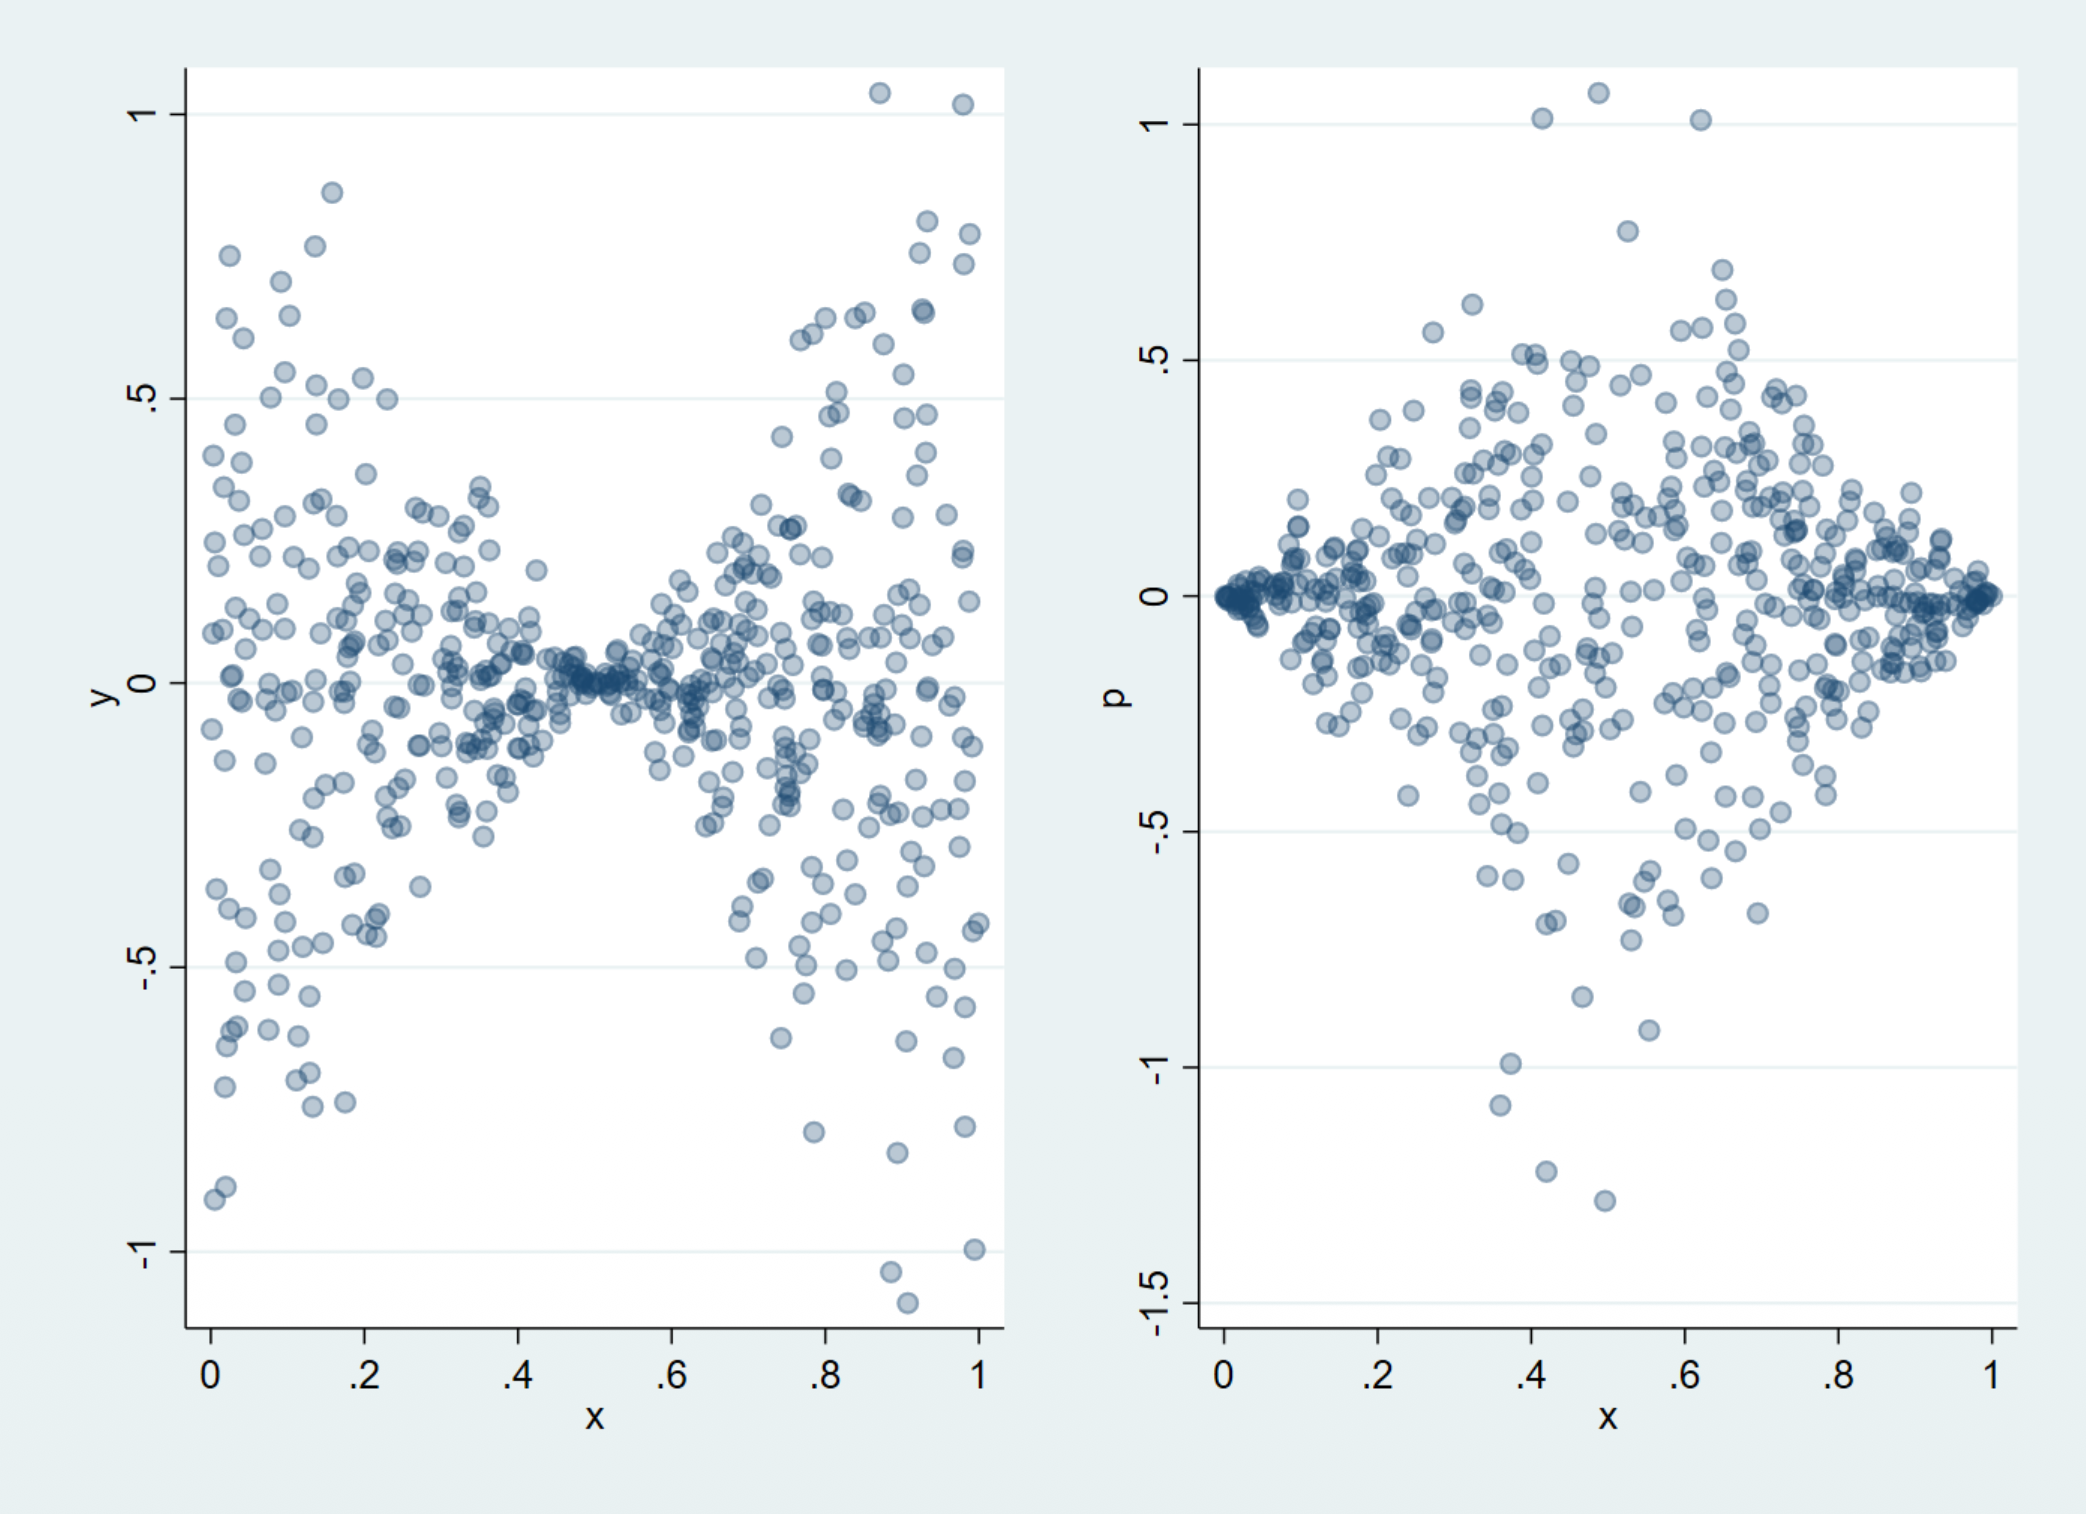
\includegraphics[width=0.78\textwidth]{images/2-12-1}
\end{figure}
Recalling a previous example, it should be much easier to estimate the slope $\beta_1$ from the data on the right, because the concentrations of mass are spread apart.
In fact, the heteroskedastic-robust standard error is smaller than the nonrobust standard error, so it is \emph{not} true that heteroskedastic-robust standard errors are always larger than nonrobust ones.

\begin{remark}	If MLR.5 holds: $\operatorname{Var}(u_i \mid x_i) = \sigma^2$. Since the error variance does not depend on the value of $x_i$, it is called homoskedastic.
	
	If the error variance depends on $x_i$, $u_i$ is heteroskedastic and MLR.5 fails.
	
	If MLR.1-4 are maintained, OLS is still unbiased and consistent under heteroskedasticity, but now the error variance depends on $x_i$: \[
		\operatorname{Var}(u_i \mid x_i) = \sigma_i^2
	,\] which in turn changes $\operatorname{Var}(\hat{\beta}_j \mid X)$.
\end{remark}

	\begin{remark}	If MLR.5 fails, and we use the wrong standard error, we may conclude that our result is significant because we mis-specified the variance of the estimator. This is why generalised least squares is not typically used and instead people do OLS with heteroskedasticity-robust standard errors (using the long form of asymptotic variance).

	Hence, while OLS will be unbiased and consistent, if we end up using the wrong test statistic in our hypothesis test, we may come to a wrong conclusion.

		We also note that using robust standard errors is valid when we have homoskedasticity, but we cannot use non-robust standard errors with heteroskedasticity. (Obviously, but we just need to emphasize this.) For example, consider the two regressions that use nonrobust and robust standard errors and the test statistic $\frac{\hat{\beta}_{\text{lotsize}}}{se\left( \hat{\beta}_{\text{lotsize}} \right)}$.
	\begin{figure}[htpb]
	  \centering
	  \begin{minipage}{0.49\textwidth}
	    \centering
	    \caption{Non-robust standard errors}
	    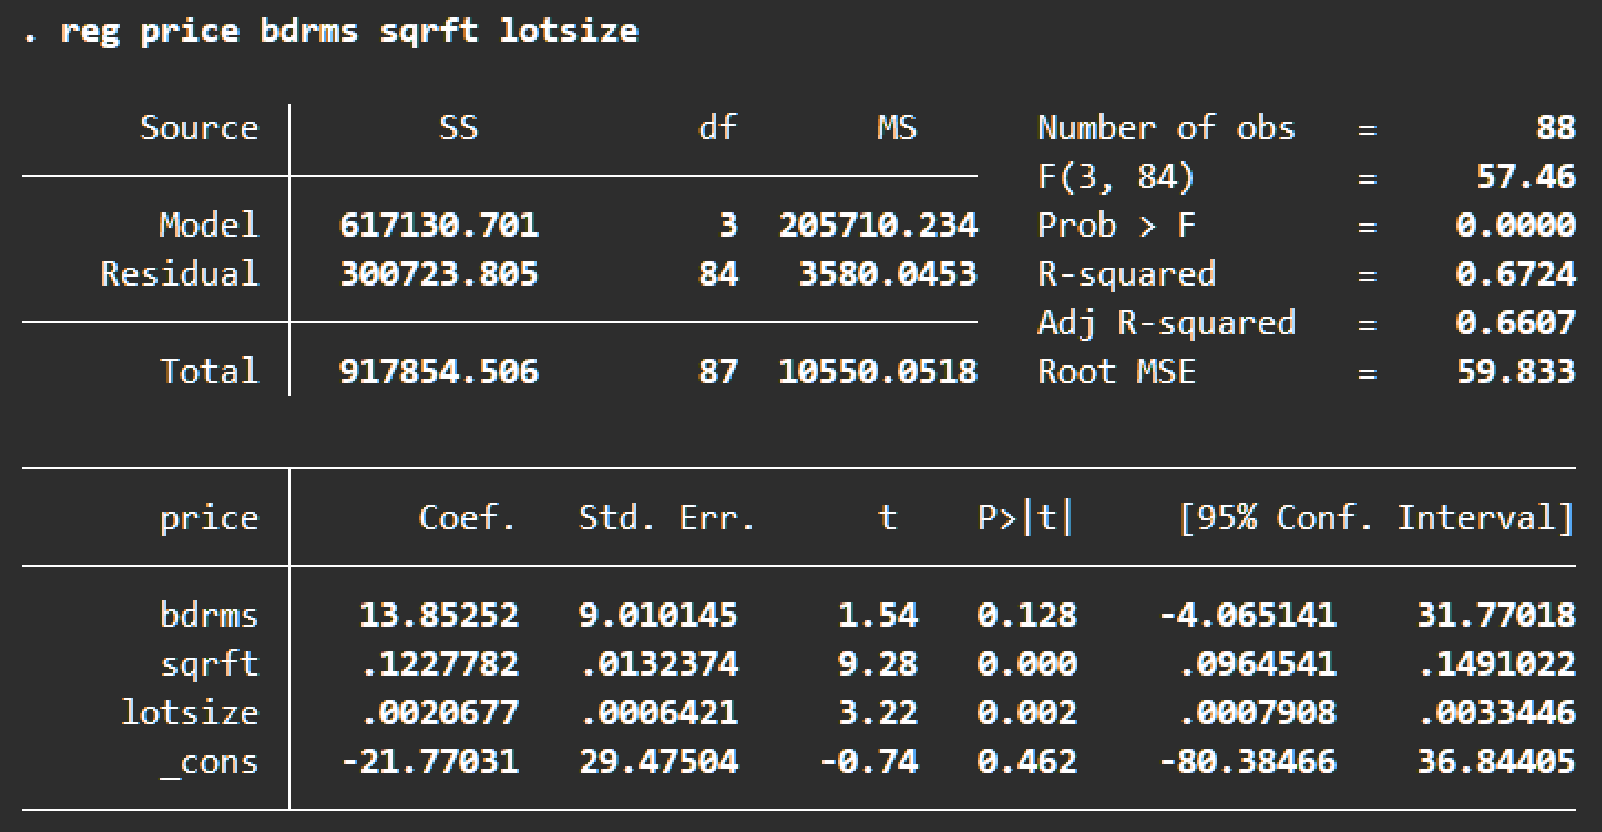
\includegraphics[width=\textwidth]{images/2-12-2}
	  \end{minipage}
	  \hfill
	  \begin{minipage}{0.49\textwidth}
	    \centering
	    \caption{Robust standard errors}
	    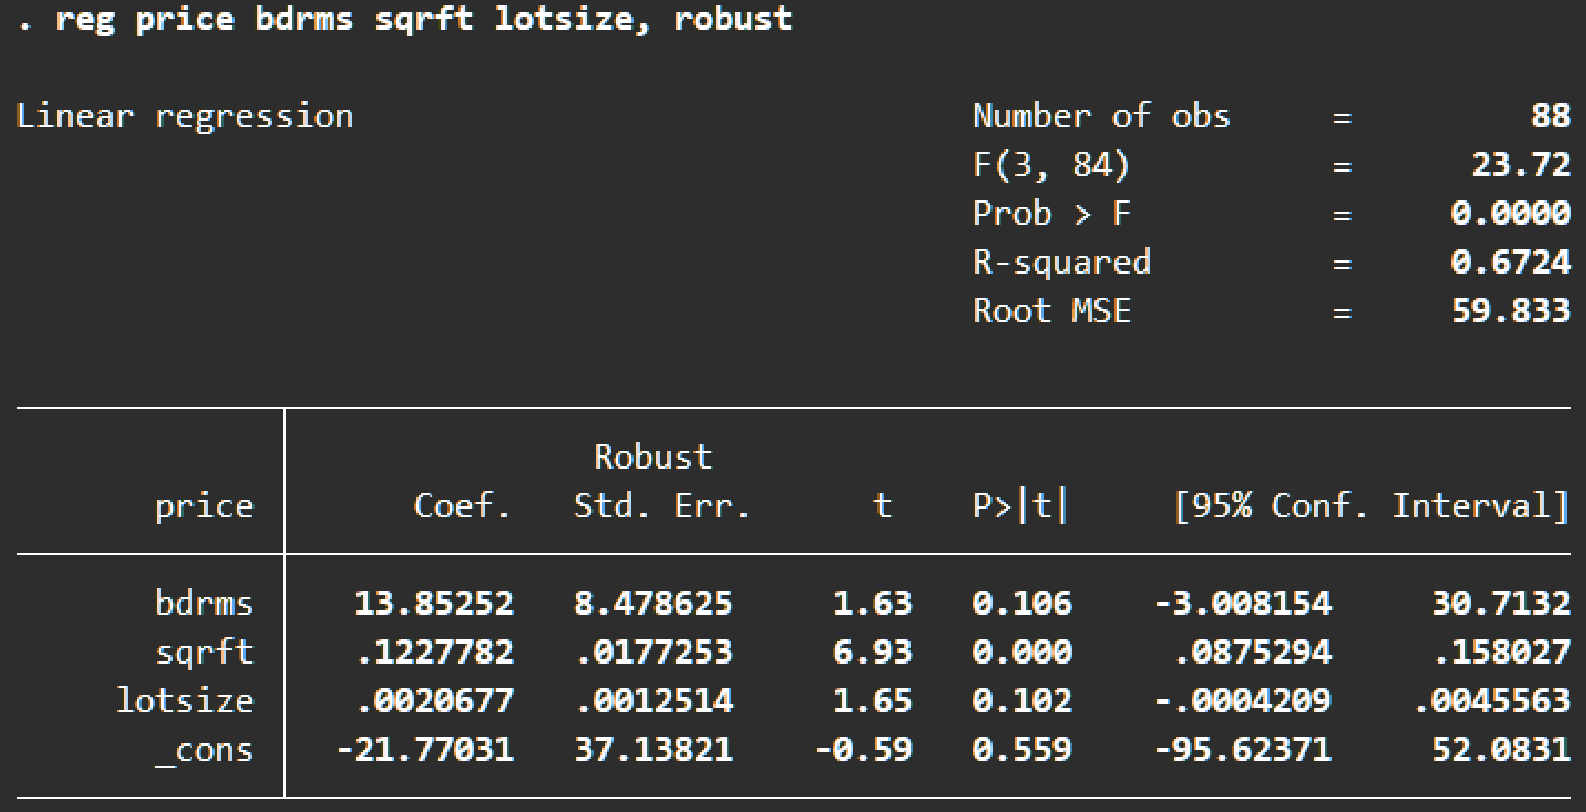
\includegraphics[width=\textwidth]{images/2-12-3}
	  \end{minipage}
	\end{figure}

	When would we ever use non-robust standard errors, then? 
	The advantage of non-robust standard errors is that $t$-stats have exact $t$-distributions under MLR.1-6.
	
	With robust standard errors, we need to use the approximation: \[
		\frac{\hat{\beta}_j - \beta_j}{\operatorname{se}_{\text{rob}}(\hat{\beta}_j)} \approx N(0,1)
	.\] 
	
	In practice, robust standard errors are used because they are valid with any form of heteroskedasticity, while justifying either of MLR.5 (homoskedasticity) or MLR.6 (normality of errors conditional on $X$) is difficult.
\end{remark}

	\begin{proposition}[Variance for individual coefficients]
		When $y_i = \beta_0 + \beta_1 x_{i1} + \cdots + \beta_k x_{ik} + u_i$, we find
		\begin{align*}
			\hat{\beta}_j = \left( X_j' M_{X_{-j}} X_j \right)^{-1} X_j' M_{X_{-j}} Y
		,\end{align*} so \[
			\hat{\beta}_j = \frac{\sum_{i=1}^{n} \hat{r}_{ij} y_i}{\sum_{i=1}^{n} \hat{r}_{ij}^2}
		,\] where $\hat{r}_{ij}$ denotes the $i$-th residual of a regression of $x_j$ on all other regressors.
	
	We find: \[
		\operatorname{Var}(\hat{\beta}_j \mid X) = \frac{\sum_{i=1}^{n} \hat{r}_{ij}^2 \operatorname{Var}(y_i \mid x_i)}{(\sum_{i=1}^{n} \hat{r}_{ij}^2)^2} = \frac{\sum_{i=1}^{n} \hat{r}_{ij}^2 \sigma_i^2}{(\sum_{i=1}^{n} \hat{r}_{ij}^2)^2}
	.\] 
	
	Because $\sigma_i^2$ is unknown, we replace it with $\E\left[u_i^2 \mid X_i\right] = \hat{u}_i^2$ and find: \[
		\widehat{\operatorname{Var}}(\hat{\beta}_j \mid X) = \frac{\sum_{i=1}^{n} \hat{r}_{ij}^2 \hat{u}_i^2}{(\sum_{i=1}^{n} \hat{r}_{ij}^2)^2}
	.\] 
	
	The heteroskedasticity robust standard error is given by\boxednote{Plugging $r_{i 1} = x_i - \overline{x}$ for a regression of $x_1$ onto a constant yields the expression we had in this section's exposition.} \[
		\operatorname{se}(\hat{\beta}_j) = \sqrt{\frac{\sum_{i=1}^{n} \hat{r}_{ij}^2 \hat{u}_i^2}{(\sum_{i=1}^{n} \hat{r}_{ij}^2)^2}}
	.\] 
\end{proposition}

\section{Weighted Least Squares}

\begin{proposition}[Weighted least squares transformation]
	If we knew the error variance $\sigma_i^2$, we could transform the model: \[
		\frac{y_i}{\sigma_i} = \left( \frac{1}{\sigma_i}, \frac{x_{i1}}{\sigma_i}, \ldots, \frac{x_{ik}}{\sigma_i} \right) \beta + \frac{u_i}{\sigma_i}
	.\] 

Notice that this model still satisfies MLR.4 since $\sigma_i$ only depends on $x_i$: \[
	\E\left( \frac{u_i}{\sigma_i} \mid x_i \right) = \frac{1}{\sigma_i} \E(u_i \mid x_i) = 0
.\] 

MLR.1-3 are unaffected, since multiplying each row of $X$ by a non-zero constant does not cause collinearity or change the interpretation of the model.

However, MLR.5 now holds, because \[
	\E\left[ \left( \frac{u_i}{\sigma_i} \right)^2 \mid \frac{x_i}{\sigma_i} \right] = \E\left[ \E\left[ \left( \frac{u_i}{\sigma_i} \right)^2 \mid x_i \right] \mid \frac{x_i}{\sigma_i} \right]
,\] and \[
	\E\left[ \left( \frac{u_i}{\sigma_i} \right)^2 \mid x_i \right] = \frac{1}{\sigma_i^2} \E(u_i^2 \mid x_i) = \frac{\sigma_i^2}{\sigma_i^2} = 1
.\] 

	OLS on the transformed model gives the best linear unbiased estimator of $\beta$ by the Gauss--Markov Theorem.\boxednote{There is some nuance here: Gauss--Markov gives us efficiency conditional on $\left(\frac{x_i}{\sigma_i}\right)$, but we will show in another problem set that it can be efficient conditional on $x$ as well.}
\end{proposition}

We really will just consider weighted least squares with homoskedasticity at the individual level. Geralized least squares weights based on the error variance, but this is beyond the scope of this course.

\begin{example}[WLS: Grouped Data]
	Suppose the model for observation $i$ is \[
		y_i = \beta_0 + \beta_1 x_i + u_i
	,\] where MLR.1-5 hold. Let $\operatorname{Var}(u \mid x) = \sigma^2$.
	
	Our observations are group averages e.g. mean age/income by zip code.
	
	There are $K$ groups $k = 1, \ldots, K$, and we observe \[
		\bar{y}_k = \frac{1}{n_k} \sum_{i \in \text{Group } k} y_i; \quad \bar{x}_k = \frac{1}{n_k} \sum_{i \in \text{Group } k} x_i
	\] for each $k = 1, \ldots, K$.
	
	We would actually run the regression on zip-code level data, so we make clear that the model written for averages is: \[
		\bar{y}_k = \beta_0 + \beta_1 \bar{x}_k + \bar{u}_k
	.\] 
	The error variance is \[
		\operatorname{Var}(\bar{u}_k \mid X) = \frac{\sigma^2}{n_k}
	.\] 
	This would actually give a different estimator of $\beta$ (since the weighting is uniform across zip codes, and not individuals as in the granular regression), and has heteroskedasticity.

	Hence, we should multiply by $\sqrt{n_k}$ to restore MLR.5\footnote{Note: we only recover homoskedasticity with this simple weighting because the original individual data was homoskedastic.} and estimate the following by OLS: \[
		\sqrt{n_k} \cdot \bar{y}_k = \beta_0 \cdot \sqrt{n_k} + \beta_1 \sqrt{n_k} \cdot \bar{x}_k + \sqrt{n_k} \cdot \bar{u}_k
	.\] 
	Here, $\operatorname{Var}(\sqrt{n_k} \cdot \bar{u}_k \mid X) = n_k \operatorname{Var}(\bar{u}_k \mid X) = \sigma^2$.
\end{example}

\section{Regression Specification}

\begin{remark}	Multiple linear regression can be used to model non-linear patterns in the data.
	
	We discuss:
	\begin{itemize}
		\item Using logarithms and polynomials to model non-linear patterns
		\item Turning continuous variables into qualitative variables
		\item Using qualitative variables to allow categories in the data to have their own coefficients
		\item Using interactions to allow the effect of changing one explanatory variable on the conditional mean to vary with the value of another.
	\end{itemize}
\end{remark}

\begin{remark}[Logarithms]
	Logarithms are often used to approximate proportional changes. For $x'$ close to $x$: \[
		\log(x') - \log(x) \approx \frac{x' - x}{x}
	\] by a first-order Taylor expansion, which is the proportional change from $x$ to $x'$.
	
	Several specifications used for conditional mean: \begin{align*}
		\E(y \mid x = t) &\approx \alpha + \beta \log(t) \quad \text{``level-log''} \\
		\E(\log(y) \mid x = t) &\approx \alpha + \beta t \quad \text{``log-level''} \\
		\E(\log(y) \mid x = t) &\approx \alpha + \beta \log(t) \quad \text{``log-log''}
	.\end{align*}
\end{remark}

Differentiating a conditional expectation is difficult, since we don't want to move the derivative operator in the expectation. Thus, the easiest log model to interpret is the log-level specification.

\begin{remark}[level-log specification]
	Consider $\E\left[y \mid x = t\right] = \alpha + \beta \ln{\left(t\right)}$.

	We have \begin{align*}
		\E(y \mid x = t + \Delta t) - \E(y \mid x = t) &\approx \beta[\log(t + \Delta t) - \log(t)] \\
		&\approx \beta \cdot \frac{\Delta t}{t} \\
		&= \frac{\beta}{100} \cdot \frac{100\Delta t}{t}
	,\end{align*} so $\beta/100$ is approximately the change in the conditional mean of $y$ when $t$ increases by $1\%$.\boxednote{This percentage interpretation is only valid for a causal interpretation, in that we examine a level of $t$ and error, then see the change in $y$ when increasing $t$. But we cannot differentiate a random variable with respect to another carelessly.}
\end{remark}

\begin{remark}[log-level specification]
	We have \[
		\E(\log(y) \mid x = t + 1) - \E(\log(y) \mid x = t) \approx \beta
	.\] 
	
		Expectations don't pass through non-linear functions (e.g. Jensen), but the following approximation leads to the common interpretation that a unit increase in $x$ is associated with a $\beta\%$ change in the mean of $y$:\boxednote{Jensen's inequality means $\E[\log y \mid x]$ need not equal $\log \E[y \mid x]$. The approximation is exact when $y \mid x$ is log-normal.} \begin{align*}
			\beta &\approx \E(\log(y) \mid x = t + 1) - \E(\log(y) \mid x = t) \\
			&\approx \log(\E(y \mid x = t + 1)) - \log(\E(y \mid x = t)) \\
			&\approx \frac{\E(y \mid x = t + 1) - \E(y \mid x = t)}{\E(y \mid x = t)}
	,\end{align*} so $100\beta$ is approximately the percentage change in the mean of $y$ resulting from a unit increase in $x$.
	
	Alternatively, exponentiating the first approximation and subtracting $1$ gives: \begin{align*}
		\exp(\beta) - 1 &\approx \exp(\E(\log(y) \mid x = t + 1) - \E(\log(y) \mid x = t)) - 1 \\
		&= \frac{\exp(\E(\log(y) \mid x = t + 1)) - \exp(\E(\log(y) \mid x = t))}{\exp(\E(\log(y) \mid x = t))}
	.\end{align*}
	Given that $\exp(x) \approx 1 + x$ when $x \approx 0$, the left hand side is approximately equal to $\beta$ if $\beta \approx 0$.
	
	We can therefore interpret $\beta$ as the proportional change in the conditional geometric mean of $y$ given a unit increase in $x$, holding the error term fixed.
\end{remark}

\begin{remark}[log-log specification]
	Now we have \[
		\E(\log(y) \mid x = t + \Delta t) - \E(\log(y) \mid x = t) \approx \beta[\log(t + \Delta t) - \log(t)]
	.\] 
	
	Combining the approximations for log-level and level-log gives: \[
		\frac{\E(y \mid x = t + \Delta t) - \E(y \mid x = t)}{\E(y \mid x = t)} \approx \beta \cdot \frac{\Delta t}{t}
	,\] so a $1\%$ increase in $t$ is associated with a $\beta\%$ change in the conditional mean of $y$ (also known as an elasticity).
\end{remark}

\begin{example}[Returns to experience]
	Consider the approximation: \[
		\E(\text{wage} \mid \text{exper}) \approx \beta_0 + \beta_1 \text{exper} + \beta_2 \text{exper}^2
	.\] 
	
	Experience estimated to have a diminishing marginal effect on wage.
	
	Turning point estimated where \[
		\frac{\partial \E(\text{wage} \mid \text{exper} = e^*)}{\partial e} = \hat{\beta}_1 + 2\hat{\beta}_2 e^* = 0 \implies e^* = -\frac{\hat{\beta}_1}{2\hat{\beta}_2} \approx 24
	.\] 
\end{example}

\begin{remark}[Returns to Experience]
	Issues with a causal interpretation:
	\begin{itemize}
		\item Omitted Variables Bias: Education impacts wage and may be correlated with/interact with exper or exper$^2$.
		\item Functional form misspecification: $w$ or $\ln(w)$? Quadratic in experience?
	\end{itemize}
	
	Average partial effect: What is the marginal effect of experience? \[
		\frac{\partial \E(\text{wage} \mid \text{exper} = e)}{\partial e} = \beta_1 + 2\beta_2 e
	.\] 
	The effect of experience diminishes if $\beta_2 < 0$. We can estimate the average partial effect: \[
		\widehat{\text{APE}} = \frac{1}{n} \sum_{i=1}^{n} (\hat{\beta}_1 + 2\hat{\beta}_2 \text{exper}_i) = \hat{\beta}_1 + 2\hat{\beta}_2 \overline{\text{exper}}_n
	.\] 
\end{remark}

\begin{remark}[Dummy Variables]
	Suppose we want to measure the difference in average wages between the tech industry and all other industries.
	
	Use a ``Dummy Variable'' to denote categories within data.
\end{remark}

\begin{remark}[Continuous variables to categorical variables]
	Suppose we are interested in estimating store sales by age category:
	\begin{itemize}
		\item Observe sales figures and age of customers.
		\item Create $k$ categories as follows: \[
			d_{i1} = \begin{cases}
				1 & \text{if } i \text{ is between 0-18 years of age} \\
				0 & \text{otherwise}
			\end{cases}
		\] \[
			d_{i2} = \begin{cases}
				1 & \text{if } i \text{ is between 18-25 years of age} \\
				0 & \text{otherwise}
			\end{cases}
		\] \[
			\vdots
		\] \[
			d_{ik} = \begin{cases}
				1 & \text{if } i \text{ is 75+ years of age} \\
				0 & \text{otherwise}
			\end{cases}
		\] 
	\end{itemize}
	
	Note: Groups are mutually exclusive ($d_{ij} d_{ik} = 0$ when $i \ne j$) and exhaustive ($d_{i1} + \cdots + d_{ik} = 1$).
	
	Means WLOG we can describe average sales by age category using \[
		\E(y_i \mid d_{i1}, \ldots, d_{ik}) = \beta_1 d_{i1} + \beta_2 d_{i2} + \cdots + \beta_k d_{ik}
	,\] where intercept is excluded to avoid perfect collinearity.
	
	Can also specify \[
		\E(y_i \mid d_{i1}, \ldots, d_{ik}) = \alpha_0 + \alpha_1 d_{i1} + \alpha_2 d_{i2} + \cdots + \alpha_{k-1} d_{ik-1}
	.\] 
	
	Note: \[
		\alpha_1 = \E(y \mid d_{i1} = 1, \ldots, d_{ik} = 0) - \E(y \mid d_{i1} = 0, \ldots, d_{ik} = 1)
	\] is interpreted as the difference in average spend between the youngest and oldest age categories.
	
	Excluding the dummy variable for the oldest category specifies that category as the base group.
	
	Intercept $\alpha_0$ is the mean for the base group.
	
	$\alpha_j$ represents difference in means between group $j$ and base group.
\end{remark}

\begin{remark}[Kinks and Jumps]
	Describe credit limits offered to new customers as a function of credit score.
	
	Sometimes outcome will change sharply at a cutoff. Suppose $y$ is credit limit and $x$ is credit score.
	
	Suppose only two categories of credit: 'Good' and 'Excellent'.
	
	Features:
	\begin{itemize}
		\item Sharp discontinuity in credit limit as soon as individual crosses 'Excellent' boundary
		\item Each additional unit of credit score improves credit limit more for individuals with excellent credit (Kink)
	\end{itemize}
	
	Let \[
		d_i = \begin{cases}
			1 & \text{if individual } x_i \ge 0.5 \\
			0 & \text{if individual } x_i < 0.5
		\end{cases}
	\] 
	
	Model: \begin{align*}
		y_i &= \beta_0 + \beta_1 x_i + d_i(\gamma + \delta x_i) + \epsilon_i \\
		&= \beta_0 + \beta_1 x_i + \gamma d_i + \delta d_i x_i + \epsilon_i
	.\end{align*}
	
	When $x_i < a$: $\E(y_i \mid x = x_i) = \beta_0 + \beta_1 x_i$.
	
	When $x_i \ge a$: $\E(y_i \mid x = x_i) = (\beta_0 + \gamma) + (\beta_1 + \delta) x_i$.
	
	Note: not all parameters have a useful interpretation: $\beta_0 + \gamma$ is the credit limit an individual with 'Excellent' credit would receive if their credit score were $0$ (We could never observe such individuals in the data).
	
	$\delta$ represents the additional return to credit score for individuals with excellent credit.
	
	Jump: $\gamma + \delta \cdot 0.5$.
\end{remark}

\begin{remark}[Saturated Regression]
	Describe wages in tech vs. not in tech, both inside and outside california: \[
		\E(W \mid T, C) = \beta_0 + \beta_1 T + \beta_2 C + \beta_3 T \cdot C
	.\] 
	We call this a saturated regression since it has one parameter for each possible value of the regressors: \[
		(T, C) \in \{(0,0), (1,0), (0,1), (1,1)\}
	.\] 
	
	The equality holds by construction, not because of an additional assumption about linearity of the conditional mean.
	
	Could also specify \[
		\E(W \mid T, C) = \alpha_0 (1-T) \cdot (1-C) + \alpha_1 T \cdot (1-C) + \alpha_2 (1-T) \cdot C + \alpha_3 T \cdot C
	.\] 
	
	Only difference is in interpretation of parameters: \begin{align*}
		\E(W \mid T = 0, C = 0) &= \beta_0 = \alpha_0 \\
		\E(W \mid T = 1, C = 0) &= \beta_0 + \beta_1 = \alpha_1 \\
		\E(W \mid T = 0, C = 1) &= \beta_0 + \beta_2 = \alpha_2 \\
		\E(W \mid T = 1, C = 1) &= \beta_0 + \beta_1 + \beta_2 + \beta_3 = \alpha_3
	.\end{align*}
	
	$\beta_1$ represents difference in average wages in tech vs. not for employees outside california.
	
	$\beta_2$ represents difference in average wages in california vs. not for employees not in tech.
	
	$\beta_3$ represents a ``difference in differences''. For example: \begin{align*}
		\beta_3 &= [(\beta_0 + \beta_1 + \beta_2 + \beta_3) - (\beta_0 + \beta_2)] - [(\beta_0 + \beta_1) - \beta_0] \\
		&= [\E(W \mid T = 1, C = 1) - \E(W \mid T = 0, C = 1)] \\
		&\quad - [\E(W \mid T = 1, C = 0) - \E(W \mid T = 0, C = 0)]
	.\end{align*}
	
	This is the difference (between california and not) in differences in wages inside and outside tech.
\end{remark}

	\begin{remark}[Interactions]
		An interaction is a product of two regressors. e.g. \[
			\text{wage} = \beta_0 + \beta_1 \text{educ} + \beta_2 \text{exper} + \beta_3 \text{educ} \cdot \text{exper} + \epsilon
	.\] 
	
		If $\E(\epsilon \mid \text{educ}, \text{exper}) = 0$, we have: \[
			\frac{\partial}{\partial \text{exper}} \E(\text{wage} \mid \text{educ}, \text{exper}) = \beta_2 + \beta_3 \text{educ}
		,\] so if $\beta_3 > 0$, average wage for those with more education differs more across experience levels.
	\end{remark}

\section{Summary}

\begin{remark}[Model and estimator]
	\leavevmode\hfill\break
	\textbf{Model}: $y = x'\beta + u$ with $\E\left[xu\right] = 0$. \\
	\textbf{Estimator}: $\hat{\beta}^{OLS} = (X'X)^{-1}X'Y$. \\
	\textbf{Interpretation}: each coefficient is the slope of the conditional mean with the remaining regressors held fixed.
\end{remark}

\begin{remark}[Finite-sample inference under normality]
	Suppose $Y \mid X \sim N(X\beta,\sigma^2 I_n)$. Exact conditional distributions:
	\[
		\begin{aligned}
			\hat{\beta} \mid X &\sim N\left(\beta,\sigma^2 (X'X)^{-1}\right), \\
			\hat{\sigma}^2 = \frac{SSR}{n-k} &\sim \frac{\sigma^2}{n-k}\chi^2_{n-k}
		\end{aligned}
	.\]
	The key finite-sample fact is that $\hat{\beta}-\beta$ and $\hat{\sigma}^2$ are conditionally independent, which yields exact $t_{n-k}$ tests and confidence intervals.
\end{remark}

\begin{remark}[Large-sample inference]
	Without normality, asymptotic normality replaces exact finite-sample formulas:
	\[
		\sqrt{n}(\hat{\beta}_n-\beta) \xrightarrow{d} N(0,V)
	.\]
	Single restrictions use asymptotic $z$-tests and confidence intervals, while multiple restrictions use $\chi^2_p$ statistics and ellipsoidal confidence sets for $R\beta$.
\end{remark}

\begin{remark}[Homoskedastic vs.\ heteroskedastic inference]
		\begin{center}
		\small
		\renewcommand{\arraystretch}{1.1}
		\begin{tabular}{p{0.20\linewidth}p{0.27\linewidth}p{0.33\linewidth}}
			\toprule
			Case & Standard error formula & Inference to use \\
			\midrule
			Homoskedastic, normal & $\hat{\sigma}^2(X'X)^{-1}$ & Exact $t$ / exact finite-sample \\
			Homoskedastic, large sample & $\hat{\sigma}^2(X'X)^{-1}$ & Asymptotic normal / $\chi^2$ \\
			Heteroskedastic & $(X'X)^{-1}X'\hat{\Omega}X(X'X)^{-1}$ & Robust asymptotic normal / $\chi^2$ \\
			\bottomrule
		\end{tabular}
		\end{center}
		Robust standard errors are valid in both homoskedastic and heteroskedastic settings, but exact $t$ inference requires the stronger homoskedastic-normal setup.
\end{remark}

\begin{remark}[Weighted least squares]
	If $\operatorname{Var}(u_i \mid x_i) = \sigma_i^2$ is known, divide the $i$-th observation by $\sigma_i$ to restore homoskedasticity. OLS on the transformed model is WLS and is efficient within the class of linear unbiased estimators under the transformed homoskedastic model.
\end{remark}

\begin{remark}[Regression specifications]
	Common specifications and their interpretation:
	\begin{itemize}
		\item \textbf{Level-log}: $\beta/100$ is the change in $\E(y \mid x)$ for a $1\%$ increase in $x$.
		\item \textbf{Log-level}: $100\beta$ approximates the percent change in $\E(y \mid x)$ for a one-unit increase in $x$.
		\item \textbf{Log-log}: $\beta$ is an elasticity.
		\item \textbf{Dummies/interactions}: allow group-specific intercepts, slopes, and difference-in-differences style comparisons.
	\end{itemize}
\end{remark}

\styledchapter{Selection on Observables}

\begin{remark}	So far we have considered counterfactuals using linear regression:
	\begin{itemize}
		\item How much does earnings potential increase with another year of experience, holding all else fixed?
		\item How much does an additional bedroom increase house price, holding floor area/lot size/air pollution (and all else) fixed?
	\end{itemize}
	OLS estimates proportional to ``partial correlations'' between outcome and regressors. ``Holding fixed'' other observable factors in this way answers counterfactual question if $y = x'\beta + u$ and $\E\left[xu\right] = 0$. In particular, $\E\left[xu\right] = 0$ implies
	\[
		\beta = \E\left[xx'\right]^{-1}\E\left[xy\right]
	,\]
	so (scaled) partial correlations are partial (causal) effects, and scaled partial correlations can be estimated.
\end{remark}

\begin{definition}[Rubin Causal Model]
	We can think about counterfactuals as `potential outcomes' under different `treatments':
	\begin{itemize}
		\item Earnings with college degree, $y(1)$, and without $y(0)$.
		\item Health outcome with drug A, $y(1)$, vs. drug B, $y(0)$.
		\item Productivity with job training, $y(1)$ vs. without, $y(0)$.
	\end{itemize}
	Define individual treatment effect for individual $i$ as $y_i(1) - y_i(0)$. Denote treatment status of individual $i$ by $D_i \in \left\{0, 1\right\}$.
\end{definition}

\section{Motivation: Store Upgrades}

Consider $100$ stores where we are trying to measure the effect of receiving an interior upgrade on sales.

\begin{example}[Store Upgrades]
	$y_i(1)$ denotes sales store $i$ would observe with an upgrade. $y_i(0)$ denotes sales store $i$ would observe without an upgrade. The outcome observed is
	\[
		Y_i =
		\begin{cases}
			y_i(1) & \text{if store $i$ is upgraded,} \\
			y_i(0) & \text{if not.}
		\end{cases}
	\]
	In other words,
	\[
		Y_i = y_i(1)D_i + y_i(0)\left(1-D_i\right)
	,\]
	where $D_i$ is an indicator for if store $i$ received an upgrade.

	We never observe the individual causal effect $y_i(1)-y_i(0)$ for any store because only one of the two potential outcomes is ever observed. However, we can try to measure average effects across treated and untreated stores by comparing averages:
	\begin{itemize}
		\item e.g. Average Treatment Effect in store population (ATE): $\E\left[y(1)-y(0)\right]$.
		\item e.g. Average Treatment Effect on the treated (ATT): $\E\left[y(1)-y(0) \mid D=1\right]$.
		\item e.g. Average Treatment Effect on untreated (ATU): $\E\left[y(1)-y(0) \mid D=0\right]$.
	\end{itemize}

	What is identified from $\E\left[Y \mid D\right]$?

	First write out the conditional mean of $Y \mid D$:
	\begin{align*}
		\E\left[Y \mid D=1\right] &= \E\left[y(1)D + y(0)(1-D) \mid D=1\right] \\
		&= \E\left[y(1) \mid D=1\right] \\
		\E\left[Y \mid D=0\right] &= \E\left[y(1)D + y(0)(1-D) \mid D=0\right] \\
		&= \E\left[y(0) \mid D=0\right]
	.\end{align*}
	We can observe $\E\left[y(1) \mid D=1\right]$ and $\E\left[y(0) \mid D=0\right]$. The data reveal an estimate of the `naive comparison':
	\[
		\E\left[y(1) \mid D=1\right] - \E\left[y(0) \mid D=0\right]
	,\]
	which is ATT plus selection effects.
\end{example}

\begin{remark}    Examining stores that are upgraded, not upgraded, and the whole population, we might see that
	\begin{center}
		\scriptsize
		\renewcommand{\arraystretch}{1.15}
		\begin{tabular}{p{0.24\linewidth}p{0.18\linewidth}p{0.18\linewidth}p{0.18\linewidth}}
			& $D_i = 0$ & $D_i = 1$ & All \\
			\hline
			average sales if upgraded
				& $\E[y(1)\mid D=0]=?$ 
				& $\E[y(1)\mid D=1]=100$
				& $\E[y(1)]=?$ \\
			average sales if not upgraded
				& $\E[y(0)\mid D=0]=50$
				& $\E[y(0)\mid D=1]=?$
				& $\E[y(0)]=?$ \\
			difference
				& $\E[y(1)-y(0)\mid D=0]=ATU$
				& $\E[y(1)-y(0)\mid D=1]=ATT$
				& $\E[y(1)-y(0)]=ATE$
		\end{tabular}
	\end{center}
\end{remark}

\begin{proposition}[Relationship between ATE, ATT, ATU]
	We can decompose the ATE as follows:
		\begin{align*}
			\E\left[y(1)-y(0)\right]
			&= \E\left[y(1)-y(0) \mid D=1\right]\P\left(D=1\right) \\
			&\quad + \E\left[y(1)-y(0) \mid D=0\right]\P\left(D=0\right) \\
			&= ATT \cdot \P\left(D=1\right) + ATU \cdot \P\left(D=0\right)
		.\end{align*}
\end{proposition}
\begin{proof}
	By the law of iterated expectation.
\end{proof}

\begin{proposition}[Regression and selection bias]
	Write out the conditional mean of $Y \mid D$:
	\[
		\E\left[Y \mid D=1\right] = \E\left[y(1) \mid D=1\right], \qquad
		\E\left[Y \mid D=0\right] = \E\left[y(0) \mid D=0\right]
	.\]
	It follows that
	\[
		\E\left[Y \mid D\right] = \beta_0 + \beta_1 D
	,\]
	where
	\[
		\beta_0 = \E\left[y(0) \mid D=0\right], \qquad
		\beta_1 = \E\left[y(1) \mid D=1\right] - \E\left[y(0) \mid D=0\right]
	.\]
\end{proposition}
\begin{proof}
	Thus $\beta_1$ equals the naive comparison. Moreover,
	\begin{align*}
		\beta_1
		&= \E\left[y(1) \mid D=1\right] - \E\left[y(0) \mid D=0\right] \\
		&= \underbrace{\E\left[y(1) \mid D=1\right] - \E\left[y(0) \mid D=1\right]}_{\text{ATT}}
		+ \underbrace{\E\left[y(0) \mid D=1\right] - \E\left[y(0) \mid D=0\right]}_{\text{Selection Bias}}
	.\end{align*}
		$\beta_1$ measures the average effect on stores that were upgraded (ATT) but is offset by ``selection bias'' in $y(0)$, which measures differences in average sales in the absence of upgrades.\boxednote{Equivalent decompositions are $\beta_1=ATT+SB_{y(0)}$ and $\beta_1=ATU+SB_{y(1)}$.}
\end{proof}

\begin{remark}	There is a big difference between selection bias in $y(0)$ vs selection bias in $y(1)$.
	
	For selection bias in $y(0)$ but not in $y(1)$, consider factories that do not get training who have scrap rates of $0.01$, factories that do get training who initially have scrap rates of $0.05$, but then $0.01$ after training.

	For selection bias in $y(1)$ but not $y(0)$, consider factories all with the same scrap rate, then factory managers who only opt into training if their employees are trainable, whose scrap rates go down after treatment. If the factories who opted out of training would have had the same scrap rate as before even if they received training, we would have selection bias in $y(1)$ only.

	Furthermore, the naive comparison can equal the ATE if the probability of selection and the magnitude of ATT/ATU cancel each other out, but this is generally not the case.
\end{remark}

\section{Random assignment}

\begin{definition}[Random assignment]
	How treatment is assigned determines whether selection bias is present. Random assignment:
	\[
		D_i \ind \left(y_i(0), y_i(1)\right)
	.\]
	This says treatment choice/assignment is independent of outcomes under treatment and no treatment.
\end{definition}

\begin{proposition}[Random assignment implies $\beta_1 = ATE$]
	Under random assignment,
	\[
		\E\left[y(0) \mid D\right] = \E\left[y(0)\right], \qquad
		\E\left[y(1) \mid D\right] = \E\left[y(1)\right]
	,\]
	i.e.\ the treatment and control groups are representative of the entire population. Hence,
	\[
		\beta_1 = \E\left[y(1)\right] - \E\left[y(0)\right] = ATE
	.\]
\end{proposition}
\begin{proof}
	\begin{align*}
		\beta_1
		&= \E\left[y(1) \mid D=1\right] - \E\left[y(0) \mid D=0\right] \text{ (naive comparison)}\\
		&= \E\left[y(1)\right] - \E\left[y(0)\right] \\
		&= ATE
	.\end{align*}
	Hence, under randomized treatment assignment, estimating a linear regression (which gives a coefficient that is the naive estimator) produces an unbiased estimate of the ATE.
\end{proof}

\begin{remark}[Multiple possible treatments]
	Suppose in a randomized clinical trial there is a control group and $k$ possible treatments for a particular health condition. Suppose participants are randomly assigned to either control or one of the treatments. Let
	\[
		x_{i1} =
		\begin{cases}
			1 & \text{if $i$ receives treatment 1,} \\
			0 & \text{otherwise,}
		\end{cases}
		\qquad
		x_{i2} =
		\begin{cases}
			1 & \text{if $i$ receives treatment 2,} \\
			0 & \text{otherwise,}
		\end{cases}
	\]
	and similarly for $x_{ik}$. There are now $k+1$ potential outcomes $y_i(0), y_i(1), \ldots, y_i(k)$ and
	\[
		Y_i = y_i(0) + x_{i1}\left(y_i(1)-y_i(0)\right) + \cdots + x_{ik}\left(y_i(k)-y_i(0)\right)
	.\]
	Now let $x_i = \left(1, x_{i1}, \ldots, x_{ik}\right)'$. We have
	\[
		\E\left[Y_i \mid x_i\right] = \beta_0 + \beta_1 x_{i1} + \cdots + \beta_k x_{ik}
	,\]
	where $\beta_0 = \E\left[y(0)\right]$ and, for each $j = 1, \ldots, k$, $\beta_j = \E\left[y(j)-y(0)\right]$.

	If we have random assignment, 
	\begin{align*}
		\E\left[Y_i \mid x_{i,1} = 0,\ldots,x_{i,k} = 0\right] &= \E\left[y_i(0) \mid x_{i,1} = 0 ,\ldots, x_{i,k} = 0\right] = \E\left[y_i(0)\right] \\
		\E\left[Y_i \mid x_{i,1} = 0 ,\ldots,x_{i,k} = 1\right] &= \E\left[y_i(k) \mid x_{i,1}= 0,\ldots,x_{i,k} = 1\right] = \E\left[y_i(k)\right] 
	.\end{align*}

	We can test whether these effects are statistically different from zero (or from each other) by forming appropriate hypotheses, e.g. $H_0:\beta_k=0$ or $H_0:\beta_1=\beta_2$.
\end{remark}

\section{Nonrandom assignment}

Now we examine when we don't have random assignment and in fact have selection bias.

\begin{example}[Job Training]
	JTRAIN98 contains data on labor market outcomes for men, some of whom enrolled in a job training program in 1997. Only men who had low earnings were allowed to enroll in the program:

	Considering the potential outcomes of earnings in 1998 without and with training, we see that the potential outcomes are correlated with treatment, because those who were eligible to be treated were lower income to begin with. (We expected both potential outcomes to be negatively correlated with $D$.) But conditioning on earnings in 1996 may remove this.

	\begin{itemize}
		\item Whether or not individual took training in 1997: $train = 1$ if training taken
		\item Earnings in 1998 (in \$1000s): $earn98$
		\item Earnings in 1996 (in \$1000s): $earn96$
		\item Whether or not individual is married: $married = 1$ if married
		\item Education in years of schooling: $educ$
		\item Age in years: $age$
	\end{itemize}
	First, compute naive comparison by running regression:
	\[
		earn98 = \beta_0 + \beta_1 train + \epsilon
	.\]Then $\hat{\beta}_1 = \overline{y}_{train} - \overline{y}_{not train} \xrightarrow{p} \E\left[Y \mid D = 1\right] - \E\left[Y \mid D = 0\right] $.
	$\hat{\beta}_1$ is a comparison of means between individuals who did/did not take training, and indicates that individuals who took training earned \$2050 less on average in 1998. This is because the selection bias is outweighing the treatment effect.

	Or, controlling for observable characteristics:
	\[
		earn98 = \beta_0 + \beta_1 train + \beta_2 educ + \beta_3 age + \beta_4 married + \beta_5 earn96 + \epsilon
	.\]

	The regression results show a negative coefficient on training when not controlling for observable characteristics, but a statistically significant positive coefficient on training when controlling for observable characteristics.
\end{example}
\begin{definition}[Covariate balance test]
	One way random assignment is justified statistically is by a ``balance test.'' We want to see if individuals with particular covariates are more likely to select into treatment. Practically: Regress treatment dummy $D_i$ on observable characteristics $x_i$:
	\[
		D_i = \gamma_0 + x_i'\gamma_1 + \epsilon_i
	.\]
	Conduct $F$-test of $H_0:\gamma_1=0$ vs. $H_1:\gamma_1 \ne 0$.\boxednote{The $F$-test is the finite sample analog of the test of multiple linear restrictions ($t$-test vs. $z$-test).}
\end{definition}

\begin{remark}[Issues with balance tests]
	The goal of a balance test is to show that $D$ is independent of potential outcomes. But this is not something that is measurable.
	A balance test can show that $x$ is uncorrelated with potential outcomes, but this is not the same thing. Both directions can fail --- there may be unobserved factors that are causally linked to the outcome, while some observables may be correlated with the outcome but have no causal relationship.

	If the significance level is 5\%, we will reject $H_0$ 5\% of the time even when $\gamma_1 = 0$. This means calling into question validity of 5\% of experimental results. If the balance test fails to reject, it doesn't mean randomization holds. $D_i$ may just be independent of observed covariates, leading to $\gamma_1 = 0$. What is really needed is
	\[
		D_i \ind \left(y_i(0), y_i(1)\right)
	.\]
\end{remark}

\begin{definition}[Unconfounded treatment assignment]
	Treatment assignment is unconfounded if, conditional on observed covariates $x_i$, treatment is as good as randomly assigned:
	\[
		D_i \ind \left(y_i(0), y_i(1)\right) \mid x_i
	.\]
	By this, we mean \[
		\P\left[D \in A, \left( y(0),y(1) \right) \in B \mid X\right] = \P\left[D \in A \mid X\right] \P\left[\left( y(0),y(1) \right) \in B \mid X\right] 
	\] for any events $A,B$. Conditional independence does not imply independence, and the converse is not true either.
\end{definition}

\begin{remark}[Conditioning on too much]
	Conditioning on too much (adding more covariates) is not always a good thing. Sometimes people argue that as long as you include all of the ``right'' covariates such that $D_i \ind \left( y_i(0), y_i(1) \right) \mid x_i$, you can add more covariates and maintain independence. But this is not true --- consider $X_{n+1}$ determining treatment assignment.
	Some machine learning fans are disappointed by this.
\end{remark}
	
\begin{example}[Selection on observables]
	Consider $W$ as earnings potential (wage) and $D = \mathds{1}_{\text{employed}}$. If we assume $W \ind D$, then $F_W(\cdot \mid D=1) = F_W(\cdot \mid D=0)$, so we could measure the population distribution of earnings potential by just looking at wages of the employed individuals.

	Now, consider a situation with a reservation wage $R$ such that $D = 1 \iff W \ge R$. Then if everyone has the same reservation wage, this independence obviously does not hold. Suppose the reservation wage is not identical and independence still holds.
	Then 
	\begin{align*}
		\E\left[W \mid D = 1, R = r\right] &= \E\left[W \mid W \ge R , R= r\right]  \\
											&= \E\left[W \mid W \ge r, R = r\right] \ge r\\
		\E\left[W \mid D=0, R = r\right]  &= \E\left[W \mid W < r, R = r\right] \\
										  &< r
	.\end{align*}
	We see that missingness at random does not imply missingness at random conditional on reservation wage. In other words, unconfoundedness may fail to hold if we condition on too much.
	
\end{example}

\begin{proposition}[Selection on observables via linear regression]
	Unconfounded treatment assignment implies
	\[
		\E\left[y(1) \mid D, x\right] = \E\left[y(1) \mid x\right], \qquad
		\E\left[y(0) \mid D, x\right] = \E\left[y(0) \mid x\right]
	,\]
	so we can estimate $\E\left[y(1) \mid D=1, x\right]$ and $\E\left[y(0) \mid D=0, x\right]$ and then estimate the ATE by aggregating over $x$.
\end{proposition}
\begin{proof}
	We see that 
	\begin{align*}
		ATE
		&= \E\left[y(1) - y(0)\right] \\
		&\overset{\text{LIE}}{=} \E\left[\E\left[y(1) - y(0) \mid X\right] \right] \\
		&= \E\left[\E\left[y(1) \mid X\right] - \E\left[y(0) \mid X\right] \right] \\
		&= \E\left[\E\left[y(1) \mid D=1,X\right] - \E\left[y(0) \mid D =0 , X\right] \right]  \text{ by unconfoundedness} \\
		&= \E\left[\E\left[Y \mid D = 1 , X\right] - \E\left[Y \mid D = 0, X\right] \right]
	.\end{align*}
	So if we can estimate $\E\left[Y \mid D=1, X\right] $, $\E\left[Y \mid D=0, X\right] $, and $F_X$, then we can estimate the ATE.
		Note that this expression is not the naive comparison, because\boxednote{The weights differ:
		$\E[Y \mid D=1]$ uses $\P(X=x \mid D=1)$, while $\E[\E[Y \mid D=1,X]]$ uses the unconditional distribution of $X$.} \[
			\E\left[Y \mid D= 1\right]  \ne \E\left[\E\left[Y \mid D=1 ,X\right] \right] 
		.\] 

	We approximated conditional means with a linear model
	\[
		\E\left[Y_i \mid D_i, x_i\right] \approx \beta_0 + \beta_1 D_i + x_i'\beta_2
	.\]
	This approximation gives
	\[
		\E\left[Y \mid D=1, x\right] - \E\left[Y \mid D=0, x\right] \approx \beta_1
	.\]
	The LIE implies that $\beta_1 = \E\left[y(1)-y(0)\right]$ (which is the ATE).

		The approximation works if\boxednote{This imposes common slopes across treated and untreated groups. It is convenient, but not necessary, for identification.}
		\[
			\E\left[y(0) \mid x\right] = \alpha_0 + x'\beta_2, \qquad
			\E\left[y(1) \mid x\right] = \alpha_1 + x'\beta_2
	,\]
	so that by the LIE,
	\[
		ATE = \E\left[y(1)-y(0)\right] = \alpha_1 - \alpha_0
	.\]
		It follows by unconfoundedness that\boxednote{Replace the observed outcome by $Y=y(0)+D(y(1)-y(0))$ and then drop the conditioning on $D$ term-by-term using unconfoundedness.}
	\begin{align*}
		\E\left[Y \mid D, x\right]
		&= \E\left[y(0) + D\left(y(1)-y(0)\right) \mid D, x\right] \\
		&= \E\left[y(0) \mid D, x\right] + D\E\left[y(1)-y(0) \mid D, x\right] \\
		&= \E\left[y(0) \mid x\right] + D\E\left[y(1)-y(0) \mid x\right] \\
		&= \alpha_0 + x'\beta_2 + D\left(\alpha_1-\alpha_0\right) \\
		&= \beta_0 + \beta_1 D + x'\beta_2
	.\end{align*}

	We turned the coefficient on $D$ from the naive comparison to the ATE.
\end{proof}

\begin{proposition}[Interaction terms and centering]
	As hinted to in the margin above, we may think that potential outcomes should have different slopes:
	\[
		\E\left[y(0) \mid x\right] = \alpha_0 + x'\beta_0, \qquad
		\E\left[y(1) \mid x\right] = \alpha_1 + x'\beta_1
	.\]
	The ATE ($\tau$) is therefore written as
	\begin{align*}
		\E\left[y(1)-y(0)\right]
		&= \E\left(\E\left[y(1) \mid x\right] - \E\left[y(0) \mid x\right]\right) \\
		&= \E\left[\left(\alpha_1-\alpha_0\right) + x'\left(\beta_1-\beta_0\right)\right]
	.\end{align*}
	Under unconfoundedness,
	\[
		\E\left[y(0) \mid D=0, x\right] = \alpha_0 + x'\beta_0, \qquad
		\E\left[y(1) \mid D=1, x\right] = \alpha_1 + x'\beta_1
	,\]
	so having different slopes changes the linear regression model:\boxednote{\begin{align*}
		Y &= y(0) + D(y(1)-y(0)) \\
		\E[Y \mid D,x] &= \E[y(0) \mid x] \\
		  &\quad{}+ D\E[y(1)-y(0) \mid x] \\
		  &= \alpha_0 + (\alpha_1-\alpha_0)D \\
		  &\quad{}+ x'\beta^0 + Dx'(\beta^1-\beta^0).
	\end{align*}}
	\[
		\E\left[Y \mid D, x\right] = \alpha_0 + \left(\alpha_1-\alpha_0\right)D + x'\beta_0 + D x'\left(\beta_1-\beta_0\right)
	.\]

	Estimating the coefficients in this model is equivalent to running two regressions:
	\begin{align*}
		Y_i &= \alpha_0 + x_i'\beta_0 \quad \text{using observations with $D_i=0$,} \\
		Y_i &= \alpha_1 + x_i'\beta_1 \quad \text{using observations with $D_i=1$.}
	.\end{align*}
	Let $\hat{y}_i(1) = \hat{\alpha}_1 + x_i'\hat{\beta}_1$ and $\hat{y}_i(0) = \hat{\alpha}_0 + x_i'\hat{\beta}_0$. Then natural to estimate $\E\left[y(1)-y(0)\right]$ as
	\[
		\hat{\tau} = \frac{1}{n}\sum\limits_{i=1}^{n}\left[\hat{y}_i(1)-\hat{y}_i(0)\right]
		= \hat{\alpha}_1 - \hat{\alpha}_0 + \bar{x}_n'\left(\hat{\beta}_1-\hat{\beta}_0\right)
	.\]

	We want the treatment effect to be the coefficient on $D$ in the combined regression, \emph{not on the interaction}. Fix: Center $x$ about $0$:
	\[
		\E\left[y(0) \mid x\right] = \delta_0 + \left(x-\mu_x\right)'\beta_0, \qquad
		\E\left[y(1) \mid x\right] = \delta_1 + \left(x-\mu_x\right)'\beta_1
	.\]
	Now the ATE is difference in intercepts:
	\[
		\E\left[y(1)-y(0)\right] = \E\left(\E\left[y(1) \mid x\right]-\E\left[y(0) \mid x\right]\right) = \delta_1-\delta_0 \equiv \tau
	.\]

	Now
	\begin{align*}
		\E\left[Y \mid D, x\right]
		&= \E\left[y(0) + D\left(y(1)-y(0)\right) \mid D, x\right] \\
		&= \E\left[y(0) \mid x\right] + D\E\left[y(1)-y(0) \mid x\right] \\
		&= \delta_0 + \tau D + \left(x-\mu_x\right)'\beta_0 + D\left(x-\mu_x\right)'\rho
	.\end{align*}
		where $\rho = \beta_1-\beta_0$. Note now that the coefficient on $D$ is $\tau = \delta_1 - \delta_0$. We don't know $\mu_x$, but replace it with $\bar{x}_n$ to obtain $\hat{\tau}$:\boxednote{Because $\bar{x}_n$ is estimated, the standard error for $\hat{\tau}$ should account for its sampling variation.}
		\[
			\begin{aligned}
				Y_i
				&= \delta_0 + \tau D_i + \left(x_i-\bar{x}_n\right)'\beta_0 \\
				&\quad + D_i\left(x_i-\bar{x}_n\right)'\rho \\
				&\quad + \epsilon_i
			\end{aligned}
		.\] 
\end{proposition}

\section{Summary}

\begin{remark}[Potential-outcomes framework]
	Potential outcomes are $y(1)$ under treatment and $y(0)$ without treatment.
	The main targets are $ATE = \E[y(1)-y(0)]$, $ATT = \E[y(1)-y(0)\mid D=1]$, and $ATU = \E[y(1)-y(0)\mid D=0]$.
	They satisfy $ATE = ATT \cdot \P(D=1) + ATU \cdot \P(D=0)$.
\end{remark}

\begin{remark}[Naive comparisons and selection bias]
	The naive regression of $Y$ on $D$ identifies
	\[
		\beta_1 = \E\left[y(1)\mid D=1\right] - \E\left[y(0)\mid D=0\right]
	.\]
	This equals $ATT$ plus selection bias in untreated potential outcomes, so a raw difference in means is not automatically causal.
\end{remark}

\begin{remark}[Random assignment]
	If $D \ind \left(y(0),y(1)\right)$, then treatment and control groups are representative of the same population:
	\[
		\E\left[y(0)\mid D\right] = \E\left[y(0)\right], \qquad
		\E\left[y(1)\mid D\right] = \E\left[y(1)\right]
	.\]
	Hence the naive comparison equals the $ATE$.
\end{remark}

\begin{remark}[Selection on observables]
	If treatment is unconfounded conditional on covariates, $D \ind \left(y(0),y(1)\right) \mid X$, then
	\[
		ATE = \E\left[\E\left[Y \mid D=1, X\right] - \E\left[Y \mid D=0, X\right]\right]
	.\]
	With the linear approximation $\E\left[Y \mid D,x\right] \approx \beta_0 + \beta_1 D + x'\beta_2$ and common slopes across treatment states, the coefficient on $D$ is the $ATE$.
\end{remark}

\begin{remark}[Different slopes and centering]
	Allowing different slopes across treatment states yields
	\[
		\E\left[Y \mid D, x\right] = \alpha_0 + \left(\alpha_1-\alpha_0\right)D + x'\beta_0 + Dx'\left(\beta_1-\beta_0\right)
	.\]
	Centering $x$ about $\mu_x$ makes the coefficient on $D$ equal to the $ATE$.
	\begin{center}
	\small
	\renewcommand{\arraystretch}{1.1}
	\begin{tabular}{p{0.22\linewidth}p{0.20\linewidth}p{0.33\linewidth}}
		\toprule
		Method & What it identifies & Key assumption \\
		\midrule
		Naive comparison & $ATT + SB$ & None \\
		Random assignment & $ATE$ & $D \ind \left(y(0),y(1)\right)$ \\
		Regression adjustment & $ATE$ & Unconfoundedness + common slopes \\
		Centered interactions & $ATE$ & Unconfoundedness + different slopes + centering \\
		\bottomrule
	\end{tabular}
	\end{center}
\end{remark}

\styledchapter{Difference-in-Differences}

\section{Example: Store Upgrades}

\begin{remark}	The common trends assumption says absent treatment, sales would follow the same trend across treated and control stores. When is this a plausible assumption? It's a counterfactual, so can't ever test it. But likely to hold if the two groups are fairly similar, or if we can add covariates to ensure they are. We can provide evidence by checking whether the two groups had similar trends before the treatment occurred (with multiple time periods).\boxednote{Note that we implicitly assume no anticipation in our notation: $Y_i(0)$ is observed for everyone for period pre-treatment, and $Y_i(1)$ is observed only for periods after the treatment time.}

	Imagine the store upgrade program happened randomly among a set of similar stores. In that context, this assumption likely holds.
\end{remark}

\begin{remark}[Data requirements]
	Comparing trends requires us to have a cross-section of outcome data before the treatment occurs, and a cross section after. Observing a random sample of observations in several time periods is called a repeated cross section. Observing the same units in several time periods is called panel data. In a repeated cross-section there is no need for the units to be the same over time. Every panel is a repeated cross-section, but not vice versa.
\end{remark}

\begin{example}[Store Upgrades setup for DiD]
	We observe sales figures $Y$ before and after upgrades for stores that were (eventually) upgraded ($G=1$) and stores that were never upgraded ($G=0$). Let $T=1$ if the sales figure is observed after upgrades, and $T=0$ otherwise. Let $y(0)$ be the sales figure we would observe without an upgrade, and $y(1)$ be the sales figure we would observe with an upgrade. Then
	\[
		Y =
		\begin{cases}
			y(1) & \text{if $G=1$, $T=1$,} \\
			y(0) & \text{otherwise.}
		\end{cases}
	\]
	We want 
	\[
		ATT = \E\left[y(1)-y(0) \mid G=1, T=1\right]
	,\]
	the effect of upgrades on sales for stores that were upgraded after they were upgraded.
\end{example}

\begin{proposition}[Before--after comparison and the trend term]
	A naive comparison across time periods gives the ATT + untreated potential outcome trend for upgraded stores.
\end{proposition}
\begin{proof}
	Comparison of means across time:
	\begin{align*}
		&\E\left[Y \mid G=1, T=1\right] - \E\left[Y \mid G=1, T=0\right] \\
		&= \E\left[Y \mid G=1, T=1\right] - \E\left[y(0) \mid G=1, T=1\right] \\
		&\quad + \E\left[y(0) \mid G=1, T=1\right] - \E\left[Y \mid G=1, T=0\right] \\
		&= \E\left[y(1)-y(0) \mid G=1, T=1\right] \\
		&\quad + \E\left[y(0) \mid G=1, T=1\right] - \E\left[y(0) \mid G=1, T=0\right]
	.\end{align*}
\end{proof}

\begin{proposition}[After-only comparison and selection bias]
	A naive comparison across groups at $T=1$ gives the ATT + differences in untreated potential outcomes across groups (selection bias).
\end{proposition}
\begin{proof}
	Comparison of means across groups after treatment:
	\begin{align*}
		&\E\left[Y \mid G=1, T=1\right] - \E\left[Y \mid G=0, T=1\right]\\
		&= \E\left[y(1) \mid G=1, T=1\right] - \E\left[y(0) \mid G=0, T=1\right] \\
		&= \E\left[y(1)-y(0) \mid G=1, T=1\right] \\
		&\quad + \E\left[y(0) \mid G=1, T=1\right] - \E\left[y(0) \mid G=0, T=1\right]
	.\end{align*}
\end{proof}

\begin{assumption}[Common Trends Assumption]
	In the absence of treatment, the trend in sales for upgraded stores and non-upgraded stores would have been the same. Formally,
	\begin{align*}
		&\E\left[y(0) \mid G=1, T=1\right] - \E\left[y(0) \mid G=1, T=0\right] \\
		&= \E\left[y(0) \mid G=0, T=1\right] - \E\left[y(0) \mid G=0, T=0\right]
	.\end{align*}
\end{assumption}

\begin{proposition}[DiD identifies the ATT]
	Now compute difference in trends for treated and control groups:
	\begin{align*}
		\text{Diff-in-Diff}
		&= \left[\E\left(Y \mid G=1, T=1\right) - \E\left(Y \mid G=1, T=0\right)\right]\\
		& \quad- \left[\E\left(Y \mid G=0, T=1\right) - \E\left(Y \mid G=0, T=0\right)\right] \\
		&= \left[\E\left(Y \mid G=1, T=1\right) - \E\left(Y \mid G=1, T=0\right)\right] \\
		&\quad - \left[\E\left(y(0) \mid G=0, T=1\right) - \E\left(y(0) \mid G=0, T=0\right)\right] \\
		&= \left[\E\left(Y \mid G=1, T=1\right) - \E\left(Y \mid G=1, T=0\right)\right] \\
		&\quad - \left[ \E\left[y(0) \mid G=1, T= 1\right] - \E\left[y(0) \mid G = 1, T = 0\right]  \right] \\
		&= ATT
	,\end{align*}
	where the second-to-last equality follows from the common trends assumption.
\end{proposition}

\begin{proposition}[Regression implementation of DiD]
	The difference-in-differences estimator is implemented by using sample averages across the four groups:
	\[
		ATT = \left[\bar{Y}_{G=1,T=1} - \bar{Y}_{G=1,T=0}\right] - \left[\bar{Y}_{G=0,T=1} - \bar{Y}_{G=0,T=0}\right]
	.\]
	We can use linear regression to generate this estimate. First, note that $\E\left[y(0) \mid G, T\right]$ can take 4 values, so WLOG:
	\[
		\E\left[y(0) \mid G, T\right] = \beta_0 + \beta_1 G + \beta_2 T + \beta_3 G \cdot T
	.\]
	The common trends assumption holds iff $\beta_3 = 0$.

	Now write the conditional mean of the observed outcome:
	\begin{align*}
		\E\left[Y \mid G, T\right]
		&= \E\left[y(0) \mid G, T\right] + \E\left[y(1)-y(0) \mid G, T\right]\cdot G \cdot T \\
		&= \E\left[y(0) \mid G, T\right] + \E\left[y(1)-y(0) \mid G=1, T=1\right]\cdot G \cdot T \\
		&= \E\left[y(0) \mid G, T\right] + ATT \cdot G \cdot T
	.\end{align*}
	since $y(1)$ is only observed if $G=T=1$. Hence
	\[
		\E\left[Y \mid G, T\right] = \beta_0 + \beta_1 G + \beta_2 T + \left[\beta_3 + ATT\right]G \cdot T
	,\]
	so under common trends, the coefficient on $G \cdot T$ is the ATT.
\end{proposition}

\begin{example}[Effect of Incinerator on Home Prices]
	Wooldridge Example 13.3: Have home values in 1978 ($y81=0$) and in 1981 ($y81=1$), when a new garbage incinerator was built. Hypothesise that house prices fell as a result of the incinerator. House defined to be near the incinerator ($nearinc$) if within 3 miles. Price ($rprice$) measured in 1978 dollars for each house. Define
	\[
		y81 =
		\begin{cases}
			1 & \text{if year = 1981} \\
			0 & \text{if year = 1978}
		\end{cases}
	.\]
	Model:
	\begin{align*}
		y
		&= \beta_0 + \beta_1 \cdot y81 + nearinc\left(\gamma_0 + \gamma_1 y81\right) + v \\
		&= \beta_0 + \beta_1 \cdot y81 + \gamma_0 nearinc + \gamma_1 y81 \cdot nearinc + v
	.\end{align*}
	Under the assumption of common trends, $\gamma_1$ is the ATT, the effect of building the incinerator on house prices near where it was built.
\end{example}

\begin{remark}[Incinerator example: selection concern]
	We could compare average house prices in 1981 across near and far. But this does not imply the incinerator caused the reduction in house prices because it might be the case that the houses in the treatment group were systematically different from the control group. The incinerator might have been built in a low-income area, where house prices would have been lower anyway.
\end{remark}

\section{Including Controls}

\begin{remark}[Including controls in DiD]
	We may include controls in main regression to:
	\begin{enumerate}[label=(\roman*)]
		\item Modify common trends assumption to hold conditional on controls.
		\item Reduce standard error on interaction term.
	\end{enumerate}
\end{remark}

\begin{assumption}[Common trends conditional on controls $X$]
	Common trends conditional on controls $X$:
	\begin{align*}
		&\E\left[y(0) \mid G=1, T=1, X=x\right] - \E\left[y(0) \mid G=1, T=0, X=x\right] \\
		&= \E\left[y(0) \mid G=0, T=1, X=x\right] - \E\left[y(0) \mid G=0, T=0, X=x\right]
	.\end{align*}
	This doesn't imply common trends because covariates can adjust over time differently for both groups.
\end{assumption}

\begin{remark}[Linearity with controls]
	If we do impose conditional common trends and linearity, then we can write
	\[
		\E\left[y(0) \mid G, T, X\right] = \beta_0 + \beta_1 G + \beta_2 T + X'\delta
	.\]
	\boxednote{This specification excludes interactions $X \times G$ and $X \times T$ by assumption. Including $X \times G$ would allow the relationship between covariates and $y(0)$ to differ between treated and control groups (e.g.\ house size matters more for treated stores). Including $X \times T$ would allow this relationship to change over time (e.g.\ the premium on house size grows post-incinerator). The no-interaction model imposes that the marginal effect of $X$ on $y(0)$ is the same across groups and time periods --- a strong but tractable restriction. Without it, one would need to explicitly interact $X$ with $G$ and $T$ in the regression, and the common trends calculation in the next line would require those additional terms to cancel as well.}
	Then
	\begin{align*}
		& \E\left[y(0) \mid G=1, T=1\right] - \E\left[y(0) \mid G=1, T=0\right]\\
		&= \beta_2 + \left[\E\left(X \mid G=1, T=1\right) - \E\left(X \mid G=1, T=0\right)\right]'\delta
	.\end{align*}
	The same calculation for $G=0$ shows that common trends only holds if the composition of covariates across time changes in the same way in both groups, or if $\delta=0$.

\end{remark}

We can write the conditional mean of the observed outcome as 
\begin{align*}
	\E\left[Y \mid G, T, X\right]
	&= \E\left[y(0) \mid G, T, X\right] + \E\left[y(1)-y(0) \mid G=1, T=1, X\right]\cdot G \cdot T \\
	&= \E\left[y(0) \mid G, T, X\right] + ATT(X)\cdot G \cdot T
.\end{align*}
since $y(1)$ is only observed if $G=T=1$. Hence
\[
	\E\left[Y \mid G, T, X\right] = \beta_0 + \beta_1 G + \beta_2 T + X'\delta + ATT(X)\cdot G \cdot T
,\]
so under conditional common trends\footnote{This is what gives the coefficient $ATT(X)$ and not $ATT(X) + \beta_3$.} and assuming a homogeneous effect across covariate values, the coefficient on $G \cdot T$ is the ATT.

If the composition of covariates doesn't change differently across groups, the standard error may still reduce significantly as a result of their inclusion. Let $\tilde{d}_i$ denote the residual from regressing $G_i T_i$ on $(1, G_i, T_i, X_i)$. By Frisch--Waugh, the variance and standard error of the ATT estimator are
\[
	\operatorname{Var}(\hat\beta_{GT} \mid G,T,X)
	= \frac{\sigma^2}{\displaystyle\sum_{i=1}^n \tilde d_i^2},
	\qquad
	\operatorname{SE}(\hat\beta_{GT})
	= \frac{\hat\sigma}{\sqrt{\displaystyle\sum_{i=1}^n \tilde d_i^2}}
.\]
More precisely, if $G \cdot T \perp X \mid G, T$ (no differential composition change), then $\tilde{d}_i$ equals the residual from projecting $G_i T_i$ on $(1, G_i, T_i)$ alone, so $\sum_i \tilde{d}_i^2$ is the same with or without $X$. We saw in homework that including more regressors weakly decreases the error variance (both population and in finite sample), so the standard error weakly decreases.

We have that $\sigma$ decreases strictly whenever $X$ has explanatory power (in sample!) for $Y$ beyond group and time indicators. Hence conditioning on $X$ \emph{always} reduces the SE under this condition, and the reduction is larger when $X$ is more predictive of $Y$.

\section{Triple Difference-in-Differences}

In the store upgrades example, parallel trends between urban and suburban stores may fail---urban stores might follow systematically different sales dynamics than suburban ones. If we observe a second city where no upgrades occurred, we can difference out these group-specific trends by running a diff-in-diff across cities.

Formally, let $G \in \{0,1\}$ denote group membership (treated subgroup vs.\ control subgroup), $T \in \{0,1\}$ denote the time period (pre vs.\ post), and $C \in \{0,1\}$ denote location (treated vs.\ control location). Treatment occurs only when $G=T=C=1$:
\[
	Y = \begin{cases} y(1) & \text{if } G=1,\ T=1,\ C=1, \\ y(0) & \text{otherwise.} \end{cases}
\]
The ATT is $\E\left[y(1)-y(0) \mid G=1, T=1, C=1\right]$.

\begin{assumption}[Common difference-in-trends across locations]
	In the absence of treatment, the difference in trends between the treated and control groups is the same across locations. Formally,
	\begin{align*}
		&\bigl[\E\left[y(0)\mid G=1,T=1,C=1\right] - \E\left[y(0)\mid G=1,T=0,C=1\right]\bigr] \\
		&\quad - \bigl[\E\left[y(0)\mid G=0,T=1,C=1\right] - \E\left[y(0)\mid G=0,T=0,C=1\right]\bigr] \\
		&= \bigl[\E\left[y(0)\mid G=1,T=1,C=0\right] - \E\left[y(0)\mid G=1,T=0,C=0\right]\bigr] \\
		&\quad - \bigl[\E\left[y(0)\mid G=0,T=1,C=0\right] - \E\left[y(0)\mid G=0,T=0,C=0\right]\bigr].
	\end{align*}
	This is weaker than requiring parallel trends within either location: group-specific trends are permitted, as long as they do not differ across locations.
\end{assumption}

\begin{proposition}[Triple difference in differences]
	We now define the ATT as
	\[
		ATT = \E\left[y(1)-y(0) \mid G=1, T=1, C=1\right]
	,\]
	where $G=1$ denotes urban stores, $C=1$ denotes city A, and $T=1$ denotes the time period after upgrades.

	Compute a diff-in-diff for city A, where treatment occured, and city B, where no treatment occurred, and difference them:
	\begin{align*}
		\E\left(Y \mid G, T, C\right)
		&= \underbrace{\beta_0 + \beta_1 G + \beta_2 T + \underbrace{\beta_3}_{\mathclap{\text{DiD, city B}}} G \cdot T}_{\text{city B base}} \\
		& \quad+ \underbrace{C\left(\gamma_0 + \gamma_1 G + \gamma_2 T + \underbrace{\left[\gamma_3 + ATT\right]}_{\mathclap{\text{DiD, city A}}}G \cdot T\right)}_{\text{deviation in city A}}
	.\end{align*}
	Under the assumption that the difference in trends is the same across the two cities, $\gamma_3 = 0$, so the triple diff-in-diff estimate of the ATT is the coefficient on $C \cdot G \cdot T$:
	\begin{align*}
		ATT &=
		\left[\bar{Y}_{G=1,T=1,C=1} - \bar{Y}_{G=1,T=0,C=1}\right]
		- \left[\bar{Y}_{G=0,T=1,C=1} - \bar{Y}_{G=0,T=0,C=1}\right]
		 \\ &- \left(
		\left[\bar{Y}_{G=1,T=1,C=0} - \bar{Y}_{G=1,T=0,C=0}\right]
		- \left[\bar{Y}_{G=0,T=1,C=0} - \bar{Y}_{G=0,T=0,C=0}\right]
		\right)
	.\end{align*}
	Running a diff in diff in $y_0$ for $C=0$ gives $\beta_3$, while on $C=1$ gives $\beta_3 + \gamma_3$, so $\gamma_3$ is the difference in violation of parallel trends. This is why we need $\gamma_3 = 0$ as the assumption for triple diff-in-diff.
\end{proposition}

\begin{remark}	Triple diff-in-diff and regular diff-in-diff produce the same estimate when there are parallel trends in both groups the triple diff-in-diff is running across.

	Both fail when there are no parallel trends in either group and the violation is different between the groups.
\end{remark}

\begin{remark}[A note on standard errors]
	Computing standard errors assuming all observations are independent may be inappropriate. Heteroskedasticity robust standard errors maintain the independence assumption. The concern is that the house price in 1978 will be correlated with its price in 1981, so we should not compute standard errors assuming independence. Often, cluster-robust standard errors are used, where a `cluster' contains groups of observations that are likely to exhibit correlation over time, or within a particular subset of the cross section (say, at the state level).
\end{remark}

\styledchapter{Instrumental Variables}

Consider the simple linear regression model \[
	y = \beta_0 + \beta_1 x_1 + u
.\]
We want to interpret $\beta_1$ as the causal effect of increasing $x_1$ by one unit on $y$, holding unobserved determinants fixed. OLS produces a scaled correlation between $x_1$ and $y$, but this is not causal unless \[
	\E\left[u\right] = \E\left[x_1 u\right] = 0
.\]
Hence, if $\E\left[x_1 u\right] \ne 0$, then $x_1$ is correlated with unobserved determinants of $y$.

\section{Simple IV Estimator}

\begin{remark}[When controls may fail]
	Control variables may not solve endogeneity when:
	\begin{itemize}
		\item We do not observe key confounders.
		\item $x_1$ is measured with error.
		\item $y$ and $x_1$ are determined simultaneously.
	\end{itemize}
	So selection on observables may be implausible if unobserved factors affect both treatment choice and outcomes.
	\boxednote{With classical measurement error in a regressor, OLS slopes are attenuated toward zero.}
\end{remark}

\begin{definition}[Exogenous, Endogenous, Instrument]
	In \[
		y = \beta_0 + \beta_1 x_1 + u
	,\]
	$x_1$ is \emph{exogenous} if $\E\left[x_1 u\right] = 0$, and \emph{endogenous} if $\E\left[x_1 u\right] \ne 0$. An instrumental variable $z$ satisfies:
	\begin{enumerate}[label=(\roman*)]
		\item \textbf{Relevance}: $\operatorname{Cov}(x_1, z) \ne 0$.
		\item \textbf{Validity}: $\operatorname{Cov}(z, u) = 0$.
		\item \textbf{Exclusion}: $z$ is not itself a determinant of $y$.
	\end{enumerate}
\end{definition}

\begin{proposition}[Why OLS is inconsistent under endogeneity]
	Consider the simple regression.
	If $\E\left[x_1 u\right] \ne 0$, then \[
		\hat{\beta}_1 = \beta_1 + \frac{\widehat{\operatorname{Cov}}(x_1, u)}{\widehat{\operatorname{Var}}(x_1)}
	,\]
	so \[
		\hat{\beta}_1 \xrightarrow{p} \beta_1 + \frac{\operatorname{Cov}(x_1, u)}{\operatorname{Var}(x_1)} = \beta_1 + \frac{\E\left[x_1 u\right]}{\operatorname{Var}(x_1)} \ne \beta_1
	,\]
	using \[
		\operatorname{Cov}(x_1, u) = \E\left[x_1 u\right] - \E\left[x_1\right]\E\left[u\right] = \E\left[x_1 u\right]
	.\]
\end{proposition}

\begin{proposition}[Simple IV identification and estimator]
	Using validity and relevance:
	\begin{align*}
		\operatorname{Cov}(z, y)
		&= \operatorname{Cov}(z, \beta_0 + \beta_1 x_1 + u) \\
		&= \beta_1 \operatorname{Cov}(z, x_1) + \operatorname{Cov}(z, u) \\
		&= \beta_1 \operatorname{Cov}(z, x_1)
	.\end{align*}
	Hence \[
		\beta_1 = \frac{\operatorname{Cov}(z, y)}{\operatorname{Cov}(z, x_1)}
	,\]
	and the sample IV estimator is \[
		\hat{\beta}_1^{IV} = \frac{\sum_{i=1}^{n}(z_i-\bar{z}_n)(y_i-\bar{y}_n)}{\sum_{i=1}^{n}(z_i-\bar{z}_n)(x_{1i}-\bar{x}_{1n})} \xrightarrow{p} \frac{\operatorname{Cov}(z, y)}{\operatorname{Cov}(z, x_1)} = \beta_1
	.\]
\end{proposition}

\begin{proposition}[Deriving the simple IV slope with and without an intercept]
	Let $x_1$ be a scalar endogenous regressor and $z$ a scalar excluded instrument.
	\begin{enumerate}[label=(\roman*)]
		\item \textbf{With an intercept.} In the structural model $y=\beta_0+\beta_1x_1+u$, using instruments $(1,z)$ yields the moment conditions $\E[u]=0$ and $\E[zu]=0$. Substituting $u=y-\beta_0-\beta_1x_1$ gives
		\[
			\E[y]-\beta_0-\beta_1\E[x_1]=0
			\quad\text{and}\quad
			\E[zy]-\beta_0\E[z]-\beta_1\E[zx_1]=0
		.\]
		Eliminate $\beta_0$ using $\beta_0=\E[y]-\beta_1\E[x_1]$:
		\begin{align*}
			0
			&= \E[zy]-\E[z]\E[y]-\beta_1\left(\E[zx_1]-\E[z]\E[x_1]\right) \\
			&= \Cov(z,y)-\beta_1\Cov(z,x_1)
		,\end{align*}
		so
		\[
			\beta_1=\frac{\Cov(z,y)}{\Cov(z,x_1)}
		.\]

		\item \textbf{No intercept.} In the structural model $y=\beta_1x_1+u$ (no constant), using the single instrument $z$ yields
		\[
			\E\!\left[z(y-\beta_1x_1)\right]=0
		,\]
		so
		\[
			\beta_1=\frac{\E[zy]}{\E[zx_1]}
			\quad\Rightarrow\quad
			\hat{\beta}_1^{IV,\;\text{no const}}=\frac{\sum_{i=1}^{n} z_i y_i}{\sum_{i=1}^{n} z_i x_{1i}}
		.\]
	\end{enumerate}
\end{proposition}

\begin{example}[Returns to education]
	Common IV application: effect of education on wages.
	\begin{enumerate}[label=(\roman*)]
		\item Schooling is a choice, so treatment may depend on unobservables.
		\item Schooling is measured with error, creating attenuation bias.
	\end{enumerate}
	A common proposed instrument is distance to nearest college: proximity affects schooling cost (relevance) but is argued not to directly determine wages (exclusion/validity).
\end{example}

\begin{remark}[Which IV conditions are testable?]
	Relevance is testable via first stage: \[
		x_1 = \pi_0 + \pi_1 z + \epsilon
	.\]
	Since \[
		\hat{\pi}_1 = \frac{\widehat{\operatorname{Cov}}(x_1, z)}{\widehat{\operatorname{Var}}(z)}
	,\]
	we can test $\pi_1=0$ with a $t$-test. Failure to reject indicates potential weak instruments.

	Validity is not directly testable with one instrument, but with multiple instruments one can run overidentification tests (the $J$-test).

	Under the maintained assumption that $z$ is valid, endogeneity of the regressor $x$ is testable via the Hausman test. This allows us to test if we need to do IV in the first place. Under $H_0:\E[xu]=0$, both OLS and IV are consistent, so $\hat{\beta}^{OLS}-\hat{\beta}^{IV}\xrightarrow{p}0$ and $\sqrt{n}(\hat{\beta}^{OLS}-\hat{\beta}^{IV})\xrightarrow{d}N(0,V)$; under $H_1:\E[xu]\ne0$, only $\hat{\beta}^{IV}$ is consistent and the gap diverges. One rejects exogeneity of $x$ at level $\alpha$ when \[
		\left|\sqrt{n}\frac{\hat{\beta}^{OLS}-\hat{\beta}^{IV}}{\sqrt{\hat{V}}}\right|>z_{1-\alpha/2}
	,\] where $\hat{V}$ is a consistent sample-analogue estimator of $\operatorname{Avar}(\hat{\beta}^{OLS}-\hat{\beta}^{IV})$, built using IV residuals $\hat{u}_i=y_i-\hat{\beta}^{IV}x_i$.
\end{remark}

\begin{proposition}[Asymptotic distribution and standard error in simple IV]
	Suppose $\E\left[u \mid z\right]=0$ and $\operatorname{Var}(u \mid z)=\sigma^2$. Then \[
		\sqrt{n}\left(\hat{\beta}_1^{IV}-\beta_1\right) \xrightarrow{d} N\left(0, \frac{\sigma^2}{\operatorname{Var}(x_1)\operatorname{Corr}(x_1,z)^2}\right)
	.\]
	Large-sample variance is approximately \[
		\frac{\sigma^2/n}{\operatorname{Var}(x_1)\operatorname{Corr}(x_1,z)^2}
	.\]
	A standard practical formula is \[
		se\left(\hat{\beta}_1^{IV}\right) = \sqrt{\frac{\hat{\sigma}^2}{SST_{x_1} \cdot R_{x_1,z}^2}}
	,\]
	where \[
		\hat{\sigma}^2 = \frac{\sum_{i=1}^{n}\left(y_i-\hat{\beta}_0^{IV}-\hat{\beta}_1^{IV}x_{1i}\right)^2}{n-2}
	.\]
	Here $SST_{x_1}=\sum_{i=1}^{n}(x_{1i}-\bar{x}_{1n})^2$ and $R_{x_1,z}^2$ is the $R^2$ from the first-stage regression $x_1=\pi_0+\pi_1 z+\epsilon$.
	Here $\hat{\sigma}^2$ must be built from IV residuals; using OLS residuals would generally be inconsistent when regressors are endogenous.

	For comparison, if $x_1$ were exogenous, OLS would satisfy \[
		\sqrt{n}\left(\hat{\beta}_1^{OLS}-\beta_1\right) \xrightarrow{d} N\left(0, \frac{\sigma^2}{\operatorname{Var}(x_1)}\right)
	.\]
	Because of the $R_{x_1,z}^2$ term, IV standard errors are typically larger than OLS standard errors.
\end{proposition}

\begin{proof}
	We can write
	\begin{align*}
		\hat{\beta}_1^{IV} - \beta_1
		&= \frac{\sum_{i=1}^{n}(z_i-\bar{z})(y_i-\bar{y})}{\sum_{i=1}^{n}(z_i-\bar{z})(x_{1i}-\bar{x}_1)} - \beta_1 \\
		&= \frac{\sum_{i=1}^{n}(z_i-\bar{z})\bigl(\beta_1(x_{1i}-\bar{x}_1)+u_i\bigr)}{\sum_{i=1}^{n}(z_i-\bar{z})(x_{1i}-\bar{x}_1)} - \beta_1 \\
		&= \frac{\sum_{i=1}^{n}(z_i-\bar{z})u_i}{\sum_{i=1}^{n}(z_i-\bar{z})(x_{1i}-\bar{x}_1)}
	.\end{align*}
	Scaling by $\sqrt{n}$,
	\[
		\sqrt{n}\bigl(\hat{\beta}_1^{IV}-\beta_1\bigr)
		= \left(\frac{1}{n}\sum_{i=1}^{n}(z_i-\bar{z})(x_{1i}-\bar{x}_1)\right)^{-1}
		\cdot \frac{1}{\sqrt{n}}\sum_{i=1}^{n}(z_i-\bar{z})u_i
	.\]
	By the LLN, the denominator converges in probability:
	\[
		\frac{1}{n}\sum_{i=1}^{n}(z_i-\bar{z})(x_{1i}-\bar{x}_1) \xrightarrow{p} \Cov(z,x_1)
	.\]
	For the numerator, $\E[u\mid z]=0$ implies $\E[zu]=0$, so the terms $(z_i-\bar{z})u_i$ are mean-zero. By the CLT and $\Var(u\mid z)=\sigma^2$,
	\[
		\frac{1}{\sqrt{n}}\sum_{i=1}^{n}(z_i-\bar{z})u_i \xrightarrow{d} N\!\left(0,\,\sigma^2\Var(z)\right)
	.\]
	By Slutsky's theorem,
	\[
		\sqrt{n}\bigl(\hat{\beta}_1^{IV}-\beta_1\bigr) \xrightarrow{d} N\!\left(0,\,\frac{\sigma^2\Var(z)}{\Cov(z,x_1)^2}\right)
	.\]
		Using $\Cov(z,x_1)^2 = \Var(z)\Var(x_1)\Corr(x_1,z)^2$ gives
		\[
			\frac{\sigma^2}{\Var(x_1)\Corr(x_1,z)^2}
		.\]
		Since $\Corr(x_1,z)^2\le 1$, the IV variance is at least as large as the OLS variance $\sigma^2/\Var(x_1)$.
		Weak instruments ($\Corr(x_1,z)\approx 0$) therefore inflate IV standard errors severely.
	\end{proof}

\begin{remark}[Weak instruments]
	Suppose the instrument barely fails validity so that $\operatorname{Cov}(z,u)$ is small but nonzero. Then the IV estimator is inconsistent: \[
		\hat{\beta}_1^{IV} \xrightarrow{p} \beta_1 + \frac{\operatorname{Cov}(z,u)}{\operatorname{Cov}(z,x_1)}
	.\]

	If the instrument is weak, in that $\Cov\left(z,x_1\right)$ is small, then the inconsistency can be large, despite the failure of validity being small. This is why it's important for:
	\begin{enumerate}[label = (\roman*)]
		\item The instrument to be valid, and
		\item The instrument to not be weak.
	\end{enumerate}
	If both fail simultaneously, the results are bad; in very weak-IV settings, finite-sample IV estimates can behave erratically and may be centered near OLS with much larger dispersion --- a strictly worse outcome.
\end{remark}

\begin{example}[Smoking and birthweight]
	Wooldridge Example 15.3: \[
		\log(\text{bwght}) = \beta_0 + \beta_1\text{packs} + u
	,\]
	where \texttt{packs} is packs smoked per day. We expect $\beta_1<0$.

	Endogeneity concern: smoking may be correlated with unobserved maternal health factors in $u$. A proposed instrument is cigarette price.
	\begin{itemize}
		\item Validity claim: cigarette prices are unrelated to unobserved determinants of birthweight.
		\item Relevance claim: cigarette prices shift smoking intensity.
	\end{itemize}
\end{example}
\boxednote{If cigarette demand is inelastic, first-stage relevance can be weak, making IV estimates very noisy in finite samples.}

\section{Sources of Endogeneity}

Consider the following setup to analyze omitted variable bias.
Suppose \[
	y = \beta_0 + \beta_1 x_1 + \beta_2 x_2 + u, \quad \E\left[u \mid x\right]=0
.\]
If $x_2$ is unobserved, we write \[
	y = \beta_0 + \beta_1 x_1 + v, \quad v=\beta_2 x_2 + u
,\]
so \[
	\operatorname{Cov}(x_1,v)=\beta_2\operatorname{Cov}(x_1,x_2)
.\]

\begin{proposition}[OVB formula]
	OLS on $y=\beta_0+\beta_1 x_1+v$ yields an estimator $\tilde{\beta}_1$ with \[
		\tilde{\beta}_1 = \hat{\beta}_1 + \hat{\beta}_2\frac{\widehat{\operatorname{Cov}}(x_1,x_2)}{\widehat{\operatorname{Var}}(x_1)}
	,\]
	and \[
		\tilde{\beta}_1 \xrightarrow{p} \beta_1 + \beta_2\frac{\operatorname{Cov}(x_1,x_2)}{\operatorname{Var}(x_1)}
	.\]
\end{proposition}

\begin{proof}
	Let $\tilde{\beta}_1 = \widehat{\Cov}(x_1,y)/\widehat{\Var}(x_1)$ be the short-regression slope. From the long regression $y = \hat{\beta}_0 + \hat{\beta}_1 x_1 + \hat{\beta}_2 x_2 + \hat{u}$, substitute into $\widehat{\Cov}(x_1,y)$:
	\begin{align*}
		\widehat{\Cov}(x_1,y)
		&= \hat{\beta}_1\widehat{\Var}(x_1) + \hat{\beta}_2\widehat{\Cov}(x_1,x_2) + \widehat{\Cov}(x_1,\hat{u})
	.\end{align*}
	By the OLS normal equations, $\widehat{\Cov}(x_1,\hat{u})=0$. Dividing by $\widehat{\Var}(x_1)$ gives the exact finite-sample identity:
	\[
		\tilde{\beta}_1 = \hat{\beta}_1 + \hat{\beta}_2\frac{\widehat{\Cov}(x_1,x_2)}{\widehat{\Var}(x_1)}
	.\]
	Taking probability limits and using consistency of $\hat{\beta}_1,\hat{\beta}_2$,
	\[
		\tilde{\beta}_1 \xrightarrow{p} \beta_1 + \beta_2\frac{\Cov(x_1,x_2)}{\Var(x_1)}
	.\]
\end{proof}

\begin{remark}[IV solution for OVB]
	Bias sign depends on $\beta_2$ and $\operatorname{Cov}(x_1,x_2)$. If both are positive, OLS tends to overestimate $\beta_1$.

	IV conditions here:
	\begin{itemize}
		\item Validity: choose $z$ uncorrelated with $v$.
		\item Relevance: in $x_1 = \gamma_0 + \gamma_1 z + \epsilon$, require $\gamma_1\ne 0$ (equivalently $\operatorname{Cov}(x_1,z)\ne 0$).
	\end{itemize}
\end{remark}

Consider the following setup to analyze measurement error.
	Let \[
		y = \beta_0 + \beta_1 x_1^* + u
	,\]
	with $\E\left[u\right]=0$, $\operatorname{Cov}(x_1^*,u)=0$. Say we observe the noisy regressor \[
		x_1 = x_1^* + v
	,\]
	where $\E\left[v\right]=0$, $\operatorname{Cov}(x_1^*,v)=0$, and $\operatorname{Cov}(u,v)=0$.

\begin{proposition}[Attenuation bias derivation]
	Rewrite as \[
		y = \beta_0 + \beta_1 x_1 + \epsilon, \quad \epsilon = u-\beta_1 v
	.\]
	Then \[
		\operatorname{Cov}(x_1,\epsilon)=\operatorname{Cov}(x_1,u-\beta_1 v)=-\beta_1\operatorname{Var}(v)
	,\]
	and OLS converges to \[
		\hat{\beta}_1^{OLS} \xrightarrow{p}  \frac{\operatorname{Cov}\left(y,x_1\right)}{\operatorname{Var}\left(x_1\right)} = \beta_1 + \frac{\operatorname{Cov}(x_1,\epsilon)}{\operatorname{Var}(x_1)} = \beta_1\left(1-\frac{\operatorname{Var}(v)}{\operatorname{Var}(x_1)}\right)
	.\]
	Also,
	\begin{align*}
		\operatorname{Var}(x_1)
		&= \operatorname{Var}(x_1^*) + \operatorname{Var}(v) + 2\operatorname{Cov}(x_1^*,v) \\
		&= \operatorname{Var}(x_1^*) + \operatorname{Var}(v) \\
		&\ge \operatorname{Var}(v)
	.\end{align*}
	Hence $1-\operatorname{Var}(v)/\operatorname{Var}(x_1)\in[0,1]$, so OLS shrinks $\beta_1$ toward zero in magnitude.
\end{proposition}

\begin{remark}[IV for measurement error]
	A possible instrument is another noisy measure:\boxednote{Think of the example with one twin estimating the other's amount of education received.} \[
		z_1 = x_1^* + w
	,\]
	with $\E\left[w\right]=0$, $\operatorname{Cov}(x_1^*,w)=0$, $\operatorname{Cov}(u,w)=0$, and $\operatorname{Cov}(w,v)=0$.

	Validity: \[
		\operatorname{Cov}(z_1,\epsilon)=\operatorname{Cov}(x_1^*+w, u-\beta_1 v)=0
	.\]
	Relevance (from first stage $x_1=\gamma_0+\gamma_1 z_1+\eta$): \[
		\operatorname{Cov}(z_1,x_1)=\operatorname{Cov}(x_1^*+w, x_1^*+v)=\operatorname{Var}(x_1^*)
	,\]
	nonzero if $x_1^*$ is not constant.
\end{remark}

\section{IV with Potential Outcomes Notation}

\begin{definition}[IV conditions in potential outcomes notation]
	We observe outcome $y$, covariates $w$, treatment status $d$, and instrument $r$. Potential outcomes are $y(d,r)$.
	\begin{enumerate}[label=(\roman*)]
		\item \textbf{Relevance}: instrument correlated with treatment (possibly conditional on covariates).
		\item \textbf{Exclusion}: for all $d,r',r''$, $y(d,r')=y(d,r'')$. So it makes sense to write $y(d) := y(d,r')$.
		\item \textbf{Exogeneity}: for all $d$, $y(d) \perp\!\!\!\perp r \mid w$.
	\end{enumerate}
\end{definition}

\begin{assumption}[Linear potential outcomes specification]
	Assume for all $d,w$: \[
		y(d)=x(w,d)'\beta + u, \quad \E\left[u \mid w\right]=0
	,\]
	with $x$ known and $\beta$ unknown constants.

	Then $\E\left[y(d)\mid w\right]$ is linear in parameters, and treatment effects are constant conditional on $w$ (two \emph{individuals} with the same observable characteristics $w$ have the same potential outcomes/treatment effects for all treatments): \[
		y(d)-y(d') = \left[x(w,d)-x(w,d')\right]'\beta
	.\]
\end{assumption}

\begin{remark}[Equivalent assumptions]
	Given the challenge describing what $u$ is and why it is constant across potential outcomes, an equivalent route is to first assume constant effects:
	\begin{enumerate}[label=(\roman*)]
		\item For all $d,w$, $\E\left[y(d)\mid w\right] = x(w,d)'\beta$.
		\item Constant effects (between individuals) conditional on $w$: for all $d,d^*$, there exists $c$ with \[
			y(d)-y(d^*) = c(w,d,d^*)
		.\]
	\end{enumerate}
	These imply that for each individual, there exists a common $u_i$ (not depending on $d$) such that \[
		y_i(d)=x(w_i,d)'\beta + u_i, \quad \E\left[u_i\mid w_i\right]=0, \quad \forall\ d
	.\]

	To see why, let $u_d = y(d)-x(w,d)'\beta$, so $\E\left[u_d \mid w\right]=0$. Using constant effects and linear conditional means gives \[
		y(d)=\left[x(w,d)-x(w,d^*)\right]'\beta + y(d^*)
	,\]
	which implies $u_d=u_{d^*}$ for all $d,d^*$. Denote this common term by $u$.\boxednote{$u$ is part projection residual and unobserved determinants of $y$.}
\end{remark}


\begin{remark}[Interpretation]
	``Linear'' means linear in parameters, not necessarily in observables: $x(w,d)$ may include nonlinear terms and interactions. Treatment effects may vary with covariates $w$, but conditional on the same $w$, effects are constant across individuals.
\end{remark}

\begin{proposition}[Observed outcome and orthogonality]
	Let $\mathcal{D}$ be the set of possible treatments and $D$ the realized treatment. Then \[
		Y = \sum_{d \in \mathcal{D}} y(d)\mathds{1}(D=d) \equiv y(D)
	,\]
	so \[
		Y = x(w,D)'\beta + u \equiv x'\beta + u
	.\]
	Since $u=y(d)-x(w,d)'\beta$ for any $d$, and $y(d) \perp\!\!\!\perp r \mid w$, we get
	\begin{align*}
		\E\left[u \mid r,w\right] 
		&= \E\left[y (d) - x(w,d)' \beta \mid r,w\right]  \\
		&= \E\left[Y(d) \mid r,w\right] - x(w,d)'\beta \\
		&= \E\left[y(d) \mid w\right]  - x(w,d)'\beta \\
		&= x(w,d)'\beta + \E\left[ u \mid w\right] - x(w,d)'\beta \\
		&= 0
	.\end{align*}
	In particular, this implies \[
		\E\left[ru\right]=0
	.\]

	The covariates are ``exogenous'' in the sense that we correctly specified the conditional mean $\E[y(d)\mid w]$: since the model holds by assumption, $u$ has zero conditional mean given $w$. This is distinct from the exogeneity of the instrument $r$, which requires the independence assumption $y(d) \ind r \mid w$. In particular, $w$ is not exogenous for the same reason $r$ is. $w$ is sometimes called a set of control variables.
	Meanwhile, $\E\left[ru\right] = 0 $ because of the exogeneity assumption on $r$ of $r \ind y(d) \mid w$.

	The covariate is valid (uncorrelated with $u$ because we correctly specify the conditional mean $y(d) \mid w$. On the other hand, $r$ must be argued to be conditionally independent of $y(d) \mid w$.
\end{proposition}

\section{General IV: Identification, Rank Condition, and Estimation}

\begin{definition}[General IV setup]
	Let $(y,x,u)$ satisfy $y=x'\beta+u$, where $y,u$ are scalar and $x\in\R^{k+1}$ with first component $x_0=1$. Let $\beta=(\beta_0,\ldots,\beta_k)'$.

	A regressor $x_j$ is exogenous if $\E\left[ux_j\right]=0$, endogenous if $\E\left[ux_j\right]\ne 0$.

	Let instruments be $z\in\R^{l+1}$ with $z_0=1$ (note that this makes $\E\left[u \right] =0$) and validity condition \[
		\E\left[zu\right]=0
	.\]
	Exogenous components of $x$ are included instruments; remaining instrument components are excluded instruments.
\end{definition}

\begin{remark}[Dimensions and notation]
	For the general IV/GMM results, stack the sample as $Y=(y_1,\ldots,y_n)'\in\R^{n}$, $X=(x_1,\ldots,x_n)'\in\R^{n\times(k+1)}$, and $Z=(z_1,\ldots,z_n)'\in\R^{n\times(l+1)}$. Define $Q=\E[z_i x_i']$ and $\Omega=\E[u_i^2 z_i z_i']$. The projection onto the instrument space is $P_Z = Z(Z'Z)^{-1}Z'$.

	Notation overload: in the omitted-variables discussion, $v$ denotes the composite error after omitting a regressor; in the measurement-error discussion, $v$ denotes the measurement error in the regressor. These are unrelated to the structural error $u$ in $y=x'\beta+u$.
\end{remark}

\begin{proposition}[Rank condition and identification]
	Assume $\E\left[zz'\right]<\infty$ and no perfect collinearity in $z$. Identification requires \[
		\operatorname{rank}\left(\E\left[zx'\right]\right)=k+1
	,\]
	the rank (relevance) condition, necessary and sufficient for unique $\beta$.

	If $l=k$ (exact identification), then \[
		\beta = \E\left[zx'\right]^{-1}\E\left[zy\right]
	.\]
\end{proposition}
\begin{proof}
	Our model is $y = x'\beta + u$. Premultiplying by $z$ and taking expectations gives
	\[
		\E\left[zy\right] = \E\left[zx'\right]\beta + \underbrace{\E\left[zu\right]}_{\mathclap{=0\text{ by validity}}}
		= Q\beta
	,\]
	where $Q=\E\left[zx'\right]$.

	Identification means the moment equation $Qb=\E[zy]$ has a unique solution $b$.

	If $\operatorname{rank}(Q)=k+1$ (full column rank), then $Qb_1=Qb_2$ implies $Q(b_1-b_2)=0$, hence $b_1=b_2$. Thus $\beta$ is uniquely determined. Equivalently, $Q'Q$ is invertible and a left inverse exists, e.g.\ $(Q'Q)^{-1}Q'$, so $\beta=(Q'Q)^{-1}Q'\E[zy]$.

	If $\operatorname{rank}(Q)<k+1$, there exists $h\ne 0$ with $Qh=0$, so both $\beta$ and $\beta+h$ satisfy $Qb=\E[zy]$. Hence $\beta$ is not identified.

	In the exactly identified case $l=k$, $Q$ is square and full rank, so $\beta = Q^{-1}\E[zy]$.
\end{proof}

\begin{proposition}[IV estimator when $l=k$]
	Sample analog: \[
		\hat{\beta}^{IV} = \left(\frac{1}{n}\sum_{i=1}^{n} z_i x_i'\right)^{-1}\left(\frac{1}{n}\sum_{i=1}^{n} z_i y_i\right) \xrightarrow{p} \E\left[zx'\right] ^{-1} \E\left[zy\right] = \beta
	.\]
	With stacked data ($Z'=(z_1,\ldots,z_n)$, $X'=(x_1,\ldots,x_n)$, $Y=(y_1,\ldots,y_n)'$), \[
		\hat{\beta}^{IV} = (Z'X)^{-1}Z'Y
	.\]
\end{proposition}

\begin{remark}[Order condition]
	A necessary condition for the rank condition is $l\ge k$.
	\begin{itemize}
		\item $l=k$: exactly identified.
		\item $l>k$: overidentified.
	\end{itemize}
	More than labeling something as overidentification and paying attention to the number of instruments vs. covariates, the rank condition that follows the next example is more important.
\end{remark}

\begin{example}[Underidentification: one excluded instrument for two endogenous regressors]
	Consider the structural equation
	\[
		y = \beta_0 + \beta_1 x_1 + \beta_2 x_2 + \beta_3 w + u
	,\]
	where $w$ is exogenous, but $x_1$ and $x_2$ are endogenous:
	\[
		\E\left[wu\right] = 0, \qquad \E\left[x_1u\right] \ne 0, \qquad \E\left[x_2u\right] \ne 0
	.\]

	Take instruments $z = (1,w,z_1)'$,
	where $z_1$ is a valid excluded instrument: $\E\left[z_1u\right]=0$.

	Then
	\[
		x = (1,x_1,x_2,w)'
	,\]
	so $x\in\R^{4}$ and $z\in\R^{3}$. Hence
	\[
		k+1 = 4, \qquad l+1 = 3
	,\]
	so $l+1<k+1$.

	The order condition fails immediately, as $\E\left[zx'\right]$
	is a $3\times 4$ matrix, so it cannot have full column rank $4$. Therefore
	\[
		\operatorname{rank}\left(\E\left[zx'\right]\right) < 4 = k+1
	,\]
	and $\beta$ is not identified.

	Intuitively, after accounting for the included exogenous regressor $w$, there is only one excluded instrument $z_1$ available to generate independent variation in the two endogenous regressors $x_1$ and $x_2$. One instrument is not enough to identify two endogenous coefficients.
\end{example}

\begin{remark}[Equivalent rank characterization]
	$\E\left[zx'\right]$ is full rank iff \[
		\E\left[zz'\right]^{-1}\E\left[zx'\right]
	\]
	is full rank. The proof is immediate by $\E\left[zz'\right] ^{-1}$ being full rank.

	If $x_j = z'\gamma_j + v_j$ with $\E\left[zv_j\right]=0$, then the $j$-th column of $\E\left[zz'\right]^{-1}\E\left[zx'\right]$ is $\gamma_j$, the first-stage linear projection coefficient vector. Stacking all $k+1$ regressors:
	\[
		\begin{aligned}
			\E\left[zz'\right]^{-1}\E\left[zx'\right]
			&= \begin{pmatrix} \gamma_0 & \gamma_1 & \cdots & \gamma_k \end{pmatrix} \\
			&= \begin{pmatrix}
				\E\left[zz'\right]^{-1} \E\left[zx_0\right] & \cdots & \E\left[zz'\right]^{-1}\E\left[zx_k\right]
			\end{pmatrix}
		\end{aligned}
	.\]
	This $(l+1)\times(k+1)$ matrix has full column rank $k+1$ if and only if $\E[zx']$ has full column rank.

	\textbf{Single endogenous regressor.} Partition $x = (x_{\text{inc}}', x_k)'$ where $x_{\text{inc}}$ are included (exogenous) regressors and $x_k$ is the single endogenous regressor, with excluded instruments $z_{\text{exc}}$. After absorbing included regressors, the rank condition reduces to $\gamma_{k,\text{exc}} \ne 0$: the excluded instruments must have a nonzero coefficient in the first-stage regression of $x_k$ on all included regressors plus the excluded instruments. The coefficients on included instruments do not affect the rank condition.

	\textbf{General case ($m_e$ endogenous regressors, $l_{\mathrm{ex}}\ge m_e$ excluded instruments).}
	Partition $z=(z_{\mathrm{in}}',z_{\mathrm{ex}}')'$ and $x=(x_{\mathrm{in}}',x_{\mathrm{en}}')'$, where $z_{\mathrm{in}}=x_{\mathrm{in}}$ collects the intercept and the $m_c$ exogenous included regressors, and $z_{\mathrm{ex}}$ collects the $l_{\mathrm{ex}}$ excluded instruments.
	Since $x_{\mathrm{in}}=z_{\mathrm{in}}$, first-stage linear projections of included regressors onto $z$ yield the identity in the top-left block and zero in the bottom-left block, giving
	\[
		\E[zz']^{-1}\E[zx'] =
		\begin{pmatrix}
			I_{m_c+1} & \Gamma_{\mathrm{in}} \\
			0         & \Gamma_{\mathrm{ex}}
		\end{pmatrix},
	\]
	where $\Gamma_{\mathrm{in}}\in\R^{(m_c+1)\times m_e}$ and $\Gamma_{\mathrm{ex}}\in\R^{l_{\mathrm{ex}}\times m_e}$ are the first-stage coefficients on included and excluded instruments, respectively, for the $m_e$ endogenous regressors.
	Subtracting $\Gamma_{\mathrm{in}}$ times the identity block from the last $m_e$ columns (which does not change rank) block-diagonalizes the matrix, so
	\[
		\operatorname{rank}(\E[zx'])=k+1 \iff \operatorname{rank}(\Gamma_{\mathrm{ex}})=m_e.
	\]
	Hence the rank condition is that the $l_{\mathrm{ex}}\times m_e$ submatrix of excluded-instrument first-stage coefficients has full column rank $m_e$.  The order condition $l_{\mathrm{ex}}\ge m_e$ is a necessary consequence.  In the exactly identified case $l_{\mathrm{ex}}=m_e$, this reduces to $\det(\Gamma_{\mathrm{ex}})\ne 0$.
\end{remark}

\begin{definition}[First stage and reduced form]
	For $x \in \R^{k+1}$, $z \in \R^{l+1}$, $v \in \R^{k+1}$, and $\pi \in \R^{(l+1)\times (k+1)}$,
	the first stage regression is: \[
		x' = z'\pi + v', \quad \E\left[zv'\right]=0
	,\]
	which is equivalently written \[
		x_j = z' \gamma_j + v_j, \quad \E\left[z v_j\right] = 0
	.\] 
	Reduced form: \[
		y = z'\delta + \epsilon, \quad \E\left[z\epsilon\right]=0
	.\]
	Under exact identification:\footnote{We use that $\left( AB \right)^{-1} = B^{-1}A^{-1}$, so we can add the $\E\left[zz'\right] ^{-1}$ terms freely.} \begin{align*}
		\beta &= \E\left[zx'\right] ^{-1} \E\left[zy\right] \\
			  &=\underbrace{\left[\E\left[zz'\right]^{-1}\E\left[zx'\right]\right]^{-1}}_{\text{First Stage Coefficients}}\underbrace{\E\left[zz'\right]^{-1}\E\left[zy\right]}_{\text{Reduced Form Coefficients}}
	.\end{align*}
\end{definition}

\begin{example}[Simultaneous equations: supply and demand]
	Consider \[
		q_D = \beta_0 + \beta_1 p + u, \quad \E\left[u\right]=0
	,\] \[
		q_S = \gamma_0 + \gamma_1 p + v, \quad \E\left[v\right]=0
	,\]
	with $\E\left[uv\right]=0$. Equilibrium $q_D=q_S$ gives \[
		p = \frac{1}{\beta_1-\gamma_1}(\gamma_0-\beta_0+v-u)
	,\]
	so \[
		\operatorname{Cov}(p,u) = -\frac{\operatorname{Var}(u)}{\beta_1-\gamma_1}, \quad \operatorname{Cov}(p,v)=\frac{\operatorname{Var}(v)}{\beta_1-\gamma_1}
	,\]
	and price is endogenous.

	Now add an exogenous supply shifter $z$: \[
		q_S = \gamma_0 + \gamma_1 p + \gamma_2 z + v, \quad \E\left[vz\right]=0, \quad \E\left[uz\right]=0
	.\]
	Then \[
		p = \frac{1}{\beta_1-\gamma_1}(\gamma_0-\beta_0+\gamma_2 z+v-u)
	,\]
	and \[
		\operatorname{Cov}(p,z) = \frac{\gamma_2\operatorname{Var}(z)}{\beta_1-\gamma_1}
	.\]
	If $\gamma_2\ne 0$, $z$ is relevant and excluded from demand, so it can identify demand parameters.
\end{example}

\section{Overidentification: Generalized Method of Moments and Two-Stage Least Squares}

\begin{remark}[Why GMM when $l>k$]
	The moment condition is\boxednote{There are $l+1$ instruments (which includes some covariates and excluded instruments) and $k+1$ covariates, which are split into exogenous and endogenous observables.} \[
		\E\left[z(y-x'\beta)\right]=0
	.\]
	When overidentified, the sample analog may have no exact solution because there are more moment equations than parameters.
	We cannot guarantee that there exists $\hat{\beta}$ such that \[
		\frac{1}{n} \sum\limits_{i=1}^{n} z_i y_i  = \frac{1}{n} \sum\limits_{i=1}^{n} z_i x_i' \hat{\beta}
	,\] 
	and this requires that the $(l+1)\times 1$ vector on the left is a linear combination of the $k+1 < l+1$ columns of $\frac{1}{n} \sum_{i=1}^{n} z_i x_i'$.

	A poor fix is discarding instruments. Better: take $k+1$ linear combinations of moments.
\end{remark}

\boxednote{\textbf{Remark 8.4.7 analogue.}
Let $Q_{zx}=\E[zx']$.

If $l=k$ and $C$ is square and invertible, then
\[
	\begin{aligned}
		Q_{zx}\text{ invertible}
		&\iff \\
		CQ_{zx}\text{ invertible}.
	\end{aligned}
\]

If $l>k$, then $Q_{zx}$ is not square, so replace invertibility by
\[
	\operatorname{rank}(Q_{zx})=k+1.
\]
Equivalently, for any fixed $W\succ0$,
\[
	Q_{zx}'WQ_{zx}
	\text{ is invertible}.
\]
To the left, for rectangular $C \in \R^{(k+1) \times (l+1)}$,
$C\in\R^{(k+1)\times(l+1)}$,
\[
	CQ_{zx}\text{ full rank}
\]
is sufficient for $Q_{zx}$ full rank of $k+1$. For a fixed $C$, it is not equivalent; $C$ could be destructive.}

\begin{definition}[Linear-combination GMM estimator]
	Let $C\in\R^{(k+1)\times(l+1)}$ with $C\E\left[zx'\right]$ full rank. By premultiplying the model by $Cz$, we have $Czy = Czx'\beta + Czu$, where $\E\left[Czx'\right] $ is square in $\R^{(k+1)\times (k+1)}$. Thus, \[
		\beta = \E\left[Czx'\right]^{-1}\E\left[Czy\right]
	,\]
	yielding multiple equivalent ways of representing $\beta$.
	Sample analog: \[
		\hat{\beta}(C) = \left(C\frac{Z'X}{n}\right)^{-1}C\frac{Z'Y}{n}
	,\]
	whenever $CZ'X$ is invertible.
\end{definition}

Above, note that if $k=l$, $C$ is square, so $\hat{\beta}(C) = \hat{\beta}_{\text{IV}}$ for all $C$.

Note that with our free choice of $C$, we have infinitely many representations of $\beta$ in the population. But using the sample analogue principle leaves us with different $\hat{\beta}$s. This is analogous to the method of moments, where representations of $\theta$ are all equal in the continuous population distribution but their analogues $\hat{\theta}$ are not equal in population.

Furthermore, we must be careful that $C$ picks out linear combinations of the instruments that satisfy the population rank condition $C\E[zx']$ being full rank---identification is a population concept, not a sample one, as asymptotic theory governs our inference.

\begin{proposition}[Consistency and asymptotic normality of GMM]
	Suppose we are given $\hat{C}\xrightarrow{p}C$. (We have not yet determined any $\hat{C}$ such that this holds.) Then \[
		\hat{\beta} = \left(\hat{C}\frac{Z'X}{n}\right)^{-1}\hat{C}\frac{Z'Y}{n} \xrightarrow{p} \beta
	.\]
	Also, \[
		\sqrt{n}(\hat{\beta}-\beta) \xrightarrow{d} N(0,V)
	,\]
	where \[
		V = \left(C\E\left[z_i x_i'\right]\right)^{-1}C\Omega C'\left(\E\left[z_i x_i'\right]'C'\right)^{-1}, \quad \Omega = \E\left[u_i^2 z_i z_i'\right]
	.\]
\end{proposition}

This formula is very very important! It is the asymptotic variance of the estimator given a $C$. Notably, it does not depend on anything other than $C$ having a consistent estimator $\hat{C}$ we can compute.

\begin{proof}
	Let $U=(u_1,\ldots,u_n)'$. Since $Y=X\beta+U$,
	\[
		\hat{\beta}
		= \left(\hat{C}\frac{Z'X}{n}\right)^{-1}\hat{C}\frac{Z'Y}{n}
		= \beta + \left(\hat{C}\frac{Z'X}{n}\right)^{-1}\hat{C}\frac{Z'U}{n}
	.\]
	By the LLN, $Z'X/n\xrightarrow{p}\E[z_i x_i']$ and $Z'U/n\xrightarrow{p}\E[z_i u_i]=0$ by validity. With $\hat{C}\xrightarrow{p}C$ and invertibility of $C\E[z_i x_i']$, it follows that $\hat{\beta}\xrightarrow{p}\beta$.

	For asymptotic normality,
	\[
		\sqrt{n}(\hat{\beta}-\beta)=\left(\hat{C}\frac{Z'X}{n}\right)^{-1}\hat{C}\frac{Z'U}{\sqrt{n}}
	.\]
	By the multivariate CLT,
	\[
		\frac{1}{\sqrt{n}}\sum_{i=1}^{n} z_i u_i \xrightarrow{d} N(0,\Omega), \quad \Omega=\E\left[u_i^2 z_i z_i'\right]
	.\]
	Slutsky's theorem gives $\sqrt{n}(\hat{\beta}-\beta)\xrightarrow{d}N(0,V)$ with
	\[
		V = \left(C\E\left[z_i x_i'\right]\right)^{-1}C\Omega C'\left(\E\left[z_i x_i'\right]'C'\right)^{-1}
	.\]
\end{proof}

\begin{proposition}[Optimal GMM weighting]
	Let $Q=\E\left[z_i x_i'\right]$ and assume $\Omega= \E\left[u_i^2 z_iz_i'\right] $ is invertible. The asymptotically optimal choice is \[
		C^{OGMM}=Q'\Omega^{-1}
	,\]
	giving \[
		V^{OGMM} = (Q'\Omega^{-1}Q)^{-1}
	.\]
	For any $C$, the difference in asymptotic covariance matrices is positive semidefinite.

	If $\hat{\Omega}\xrightarrow{p}\Omega$, the feasible optimal GMM is \[
		\hat{\beta}^{OGMM} = (\overbrace{X'Z\hat{\Omega}^{-1}}^{n \hat{C}}Z'X)^{-1}\overbrace{X'Z\hat{\Omega}^{-1}}^{n \hat{C}}Z'Y
	,\]
	with \[
		\sqrt{n}(\hat{\beta}^{OGMM}-\beta) \xrightarrow{d} N\left(0,(Q'\Omega^{-1}Q)^{-1}\right)
	.\]
\end{proposition}

\begin{proof}
	Let $R = \Omega^{-1/2}Q$ where $\Omega^{1/2}$ is the symmetric positive-definite square root of $\Omega$.

	\textbf{Step 1: Verify $V^{OGMM}$.} Substituting $C^{OGMM} = Q'\Omega^{-1}$ into $V(C)$:
	\begin{align*}
		V(C^{OGMM})
		&= (Q'\Omega^{-1}Q)^{-1}Q'\Omega^{-1}\cdot\Omega\cdot\Omega^{-1}Q(Q'\Omega^{-1}Q)^{-1} \\
		&= (Q'\Omega^{-1}Q)^{-1}
	.\end{align*}

	\textbf{Step 2: Show $V(C) - V^{OGMM} \succeq 0$.} Let $B = C\Omega^{1/2}$. Use the orthogonal decomposition $I = R(R'R)^{-1}R' + M_R$ where $M_R = I - R(R'R)^{-1}R'$ is the residual maker of $R$:
	\begin{align*}
		BB' &= C\Omega^{1/2}\bigl[R(R'R)^{-1}R' + M_R\bigr]\Omega^{1/2}C' \\
			&= CQ(Q'\Omega^{-1}Q)^{-1}Q'C' + C\Omega^{1/2}M_R\Omega^{1/2}C'
	,\end{align*}
	using $\Omega^{1/2}R = Q$. Writing $V(C) = (CQ)^{-1}BB'(Q'C')^{-1}$ and substituting:
	\begin{align*}
		V(C)
		&= (Q'\Omega^{-1}Q)^{-1} + (CQ)^{-1}C\Omega^{1/2}M_R\Omega^{1/2}C'(Q'C')^{-1}
	.\end{align*}
	Since $M_R$ is symmetric and idempotent, $M_R \succeq 0$, so $C\Omega^{1/2}M_R\Omega^{1/2}C' \succeq 0$, hence
	\[
		V(C) - V^{OGMM} = (CQ)^{-1}C\Omega^{1/2}M_R\Omega^{1/2}C'(Q'C')^{-1} \succeq 0
	.\]
	This is the same projection argument as in the Gauss--Markov theorem.
\end{proof}

Hence, the asymptotically optimal linear combination of moments is found by setting \[
	\hat{\beta} = \left( \hat{C} Z' X \right)^{-1} \hat{C} Z' Y
,\] where $\hat{C}$ is a consistent estimator of $\E\left[z_i x_i'\right] \Omega^{-1}$. The first term is easy to estimate, but $\Omega^{-1} = \E\left[u_i^2 z_i z_i'\right] ^{-1}$ is difficult to estimate.

\begin{proposition}[Conditional homoskedasticity and 2 Stage Least-Squares]
	If $\E\left[u\mid z\right]=0$ and $\E\left[u^2\mid z\right]=\sigma^2$, then \[
		\Omega = \E\left[u^2 zz'\right] = \sigma^2\E\left[zz'\right]
	.\]
	So feasible optimal GMM becomes \[
		\hat{\beta}^{OGMM} =  (X'P_ZX)^{-1}X'P_ZY =: \hat{\beta}^{2SLS}, \quad P_Z = Z(Z'Z)^{-1}Z'
	.\]

	The interpretation of two-stage least squares is as follows:
	\begin{enumerate}[label=(\roman*)]
		\item First stage: regress each column of $X$ on $Z$, so $P_ZX=Z\hat{\Pi}$.
		\item Second stage: regress $Y$ on $P_ZX$.
	\end{enumerate}
	Included instruments are unchanged by projection. If $l=k$, $\hat{\beta}^{2SLS}=\hat{\beta}^{IV}$.

	In the first stage, we do prediction on the model $x' = z' \Pi + v'$, or $x = \Pi' z + v$ and find the error minimizer $\hat{\Pi}$ to solve in matrix form \[
		X = Z \hat{\Pi} + V
	.\] This yields $\hat{\Pi} = (Z'Z)^{-1}Z'X$, and we put $P_Z X = Z\hat{\Pi}$.
\end{proposition}

\begin{proof}
	Under $\E[u^2\mid z]=\sigma^2$, we have $\Omega = \sigma^2\E[z_iz_i']$. Substituting $\hat{\Omega} = \hat{\sigma}^2(Z'Z/n)$ into the OGMM formula and cancelling $\hat{\sigma}^2$:
	\begin{align*}
		\hat{\beta}^{OGMM}
		&= \left( X'Z \left[ \hat{\sigma}^2 \frac{Z'Z}{n} \right]^{-1} Z'X \right)^{-1} X'Z \left[ \hat{\sigma}^2\frac{Z'Z}{n} \right]^{-1} Z' Y \\
		&= \left( X'Z (Z'Z)^{-1} Z'X \right)^{-1} X'Z (Z'Z)^{-1} Z' Y \\
		&= \left( X'P_Z X \right)^{-1} X'P_ZY =: \hat{\beta}^{2SLS}
	.\end{align*}
	The definition of $\hat{\beta}^{2SLS}$ comes from the following procedure: the first stage regresses each column of $X$ on $Z$: $P_Z X = Z\hat{\Pi}$, where $\hat{\Pi} = (Z'Z)^{-1}Z'X$. The second stage regresses $Y$ on $P_Z X$, the projection of $X$ onto the instrument space.

	When $l=k$ (exact identification), $Z'Z$ and $Z'X$ are square. Let $A=Z'X$ and $B=(Z'Z)^{-1}$. Then
	\[
		\hat{\beta}^{2SLS} = (A'BA)^{-1}A'BZ'Y
	.\]
	Since $(A'BA)^{-1}A'B$ is a left inverse of $A$ and $A$ is invertible under the rank condition, it equals $A^{-1}$. Hence $\hat{\beta}^{2SLS} = (Z'X)^{-1}Z'Y = \hat{\beta}^{IV}$.
\end{proof}

Under conditional homoskedasticity, the optimal weighting matrix leads to $C^{2SLS} = [\E[zz']^{-1}\E[zx']]'$. Concretely, the first-stage fitted values $P_Z X$ are the optimal linear combinations of the instruments: regressing $X$ on $Z$ extracts the variation in $X$ that is explained by and therefore exogenous to $Z$.

Under conditional homoskedasticity, adding valid and relevant instruments can reduce 2SLS standard errors by enlarging the instrument space and thereby increasing the exogenous variation in $X$ captured by the first stage. In matrix terms, this works through an increase in $X'P_ZX$, which lowers the homoskedastic variance formula $n\hat{\sigma}^2(X'P_ZX)^{-1}$. In the special case of a single endogenous regressor, this appears as a higher first-stage $R^2$; with several endogenous regressors, there is no single scalar $R^2$ governing all standard errors. However, when $l$ is large relative to $n$, the first-stage projection overfits: $P_Z X \approx X$, and 2SLS approaches OLS. There is therefore a tradeoff between adding instruments (variance reduction from a stronger first stage) and overfitting (finite-sample bias when instruments are numerous but weak).

In the second stage, the exogenous regressors in $X$ are unchanged by $P_Z$, while the endogenous regressors are replaced by their projections onto the column space of the instruments. This removes the endogenous component from the regressors.

The \emph{only} thing that heteroskedasticity changes is the asymptotic variance of $\hat{\beta}^{OGMM}$. Under homoskedasticity, $\hat{\beta}^{OGMM} = \hat{\beta}^{2SLS}$. Under heteroskedasticity, $\hat{\beta}^{2SLS}$ is no longer the asymptotically efficient GMM estimator, but it remains consistent and asymptotically normal.

\begin{proposition}[Asymptotic distribution and inference for 2SLS]
	Under conditional homoskedasticity, \[
		\sqrt{n}(\hat{\beta}^{2SLS}-\beta) \xrightarrow{d} N\left(0, \sigma^2\left(Q'\E\left[z_i z_i'\right]^{-1}Q\right)^{-1}\right)
	.\]
	With $\hat{U}=Y-X\hat{\beta}^{2SLS}$, a consistent estimator is \[
		\hat{\sigma}^2 = \frac{\hat{U}'\hat{U}}{n}
	.\]
	Then \[
		\hat{V}^{hom} = n\hat{\sigma}^2(X'P_ZX)^{-1}
	.\]
	For any constant vector $r\in\R^{k+1}$, \[
		\frac{\sqrt{n}\,r'\left(\hat{\beta}^{2SLS}-\beta\right)}{\sqrt{r'\hat{V}^{hom}r}} \xrightarrow{d} N(0,1)
	,\]
	which gives confidence sets and tests.
\end{proposition}
\begin{proof}
	The general GMM asymptotic variance is $(Q'\Omega^{-1}Q)^{-1}$.
	Under homoskedasticity $\Omega = \sigma^2\E[zz']$, so substituting $\Omega^{-1}$:
	\[
		V^{hom} = \left(Q'\cdot\sigma^{-2}\E[zz']^{-1}\cdot Q\right)^{-1} = \sigma^2\left(Q'\E[zz']^{-1}Q\right)^{-1}
	,\]
	which matches the stated expression.

	To see that $\hat{\sigma}^2=\hat{U}'\hat{U}/n$ is consistent, write
	\[\hat{U}=Y-X\hat{\beta}^{2SLS}=U-X(\hat{\beta}^{2SLS}-\beta).\]
	Expanding,
	\[
		\frac{\hat{U}'\hat{U}}{n}
		= \frac{U'U}{n}
		-2(\hat{\beta}^{2SLS}-\beta)'\frac{X'U}{n}
		+(\hat{\beta}^{2SLS}-\beta)'\frac{X'X}{n}(\hat{\beta}^{2SLS}-\beta)
	.\]
	Since $\hat{\beta}^{2SLS}-\beta=O_p(n^{-1/2})$ and $X'U/n$ and $X'X/n$ are $O_p(1)$, the last two terms are $o_p(1)$, so $\hat{\sigma}^2=U'U/n+o_p(1)\xrightarrow{p}\E[u_i^2]=\sigma^2$.

	For the consistent estimator, rescaling gives
	\begin{align*}
		\hat{V}^{hom} &= \hat{\sigma}^2 \left( \frac{X'Z}{n}\left( \frac{Z'Z}{n} \right)^{-1} \left( \frac{Z'X}{n} \right) \right)^{-1}\\
		&= n\hat{\sigma}^2 \left( X'Z \left( Z'Z \right)^{-1}Z'X \right)^{-1}
	.\end{align*}
	
	The convergence expression follows from
	\begin{align*}
		r' \left( \sqrt{n} \left( \hat{\beta}^{2SLS} - \beta \right) \right)
		&\xrightarrow{d} r' N\left( 0, V^{hom} \right)\\
		&\overset{d}{=} N\left( 0, r' V^{hom}r \right)
	.\end{align*}
\end{proof}

Importantly, $\hat{U}$ must be estimated using $\hat{\beta}^{2SLS}$ because $\hat{\beta}^{OLS}$ is inconsistent, which leaves us with something that does not converge to $0$. 

\begin{proposition}[Heteroskedasticity and feasible optimal GMM]
	Under heteroskedasticity, estimate \[
		\hat{\Omega} = \frac{1}{n}\sum_{i=1}^{n}\hat{u}_i^2 z_i z_i', \quad \hat{u}_i = y_i - x_i'\hat{\beta}^{2SLS}
	.\]
	Then optimal feasible GMM is \[
		\hat{\beta}^{OGMM} = (X'Z\hat{\Omega}^{-1}Z'X)^{-1}X'Z\hat{\Omega}^{-1}Z'Y
	,\]
	and \[
		\sqrt{n}(\hat{\beta}^{OGMM}-\beta) \xrightarrow{d} N(0,V^{het}), \quad V^{het} = (Q'\Omega^{-1}Q)^{-1}
	.\]
	A consistent estimator is \[
		\hat{V}^{het} = \left(\frac{X'Z}{n}\hat{\Omega}^{-1}\frac{Z'X}{n}\right)^{-1}
	.\]
\end{proposition}

\begin{proof}
	\textbf{Step 1: Consistency of $\hat{\Omega}$.} Since $\hat{\beta}^{2SLS}\xrightarrow{p}\beta$, we have $\hat{u}_i=y_i-x_i'\hat{\beta}^{2SLS}=u_i-x_i'(\hat{\beta}^{2SLS}-\beta)\xrightarrow{p}u_i$. Under finite-moment assumptions, the LLN gives
	\[
		\hat{\Omega}=\frac{1}{n}\sum_{i=1}^{n}\hat{u}_i^2 z_i z_i' \xrightarrow{p} \E\left[u_i^2 z_i z_i'\right]=\Omega
	.\]

	\textbf{Step 2: Consistency of the estimated weighting.} If $\Omega$ is invertible, then $\hat{\Omega}^{-1}\xrightarrow{p}\Omega^{-1}$ by continuous mapping. Also $X'Z/n\xrightarrow{p}Q'$. Hence
	\[
		\hat{C}^{OGMM}:=\frac{X'Z}{n}\hat{\Omega}^{-1}\xrightarrow{p}Q'\Omega^{-1}=C^{OGMM}
	.\]

	\textbf{Step 3: Asymptotic normality.} Write the feasible OGMM estimator in the linear-combination form with $\hat{C}^{OGMM}$:
	\[
		\hat{\beta}^{OGMM}=\left(\hat{C}^{OGMM}\frac{Z'X}{n}\right)^{-1}\hat{C}^{OGMM}\frac{Z'Y}{n}
	.\]
	Since $\hat{C}^{OGMM}\xrightarrow{p}C^{OGMM}$, the general GMM asymptotic normality result gives
	\[
		\sqrt{n}(\hat{\beta}^{OGMM}-\beta)\xrightarrow{d}N(0,V(C^{OGMM}))
	.\]
	With $C^{OGMM}=Q'\Omega^{-1}$, optimality implies $V(C^{OGMM})=(Q'\Omega^{-1}Q)^{-1}=V^{het}$.

	\textbf{Step 4: Consistency of $\hat{V}^{het}$.} Using $X'Z/n\xrightarrow{p}Q'$, $Z'X/n\xrightarrow{p}Q$, and $\hat{\Omega}^{-1}\xrightarrow{p}\Omega^{-1}$,
	\[
		\hat{V}^{het}=\left(\frac{X'Z}{n}\hat{\Omega}^{-1}\frac{Z'X}{n}\right)^{-1}\xrightarrow{p}(Q'\Omega^{-1}Q)^{-1}=V^{het}
	.\]
\end{proof}

Note that the feasible $\hat{\beta}^{OGMM}$ depends on $\hat{\Omega}$, and $\hat{\Omega}$ depends on residuals $\hat{u}_i = y_i - x_i'\hat{\beta}$. This creates a circularity. A standard approach is 2-step GMM: compute $\hat{\beta}^{2SLS}$, build $\hat{\Omega}$ from $\hat{u}_i = y_i - x_i'\hat{\beta}^{2SLS}$, then compute $\hat{\beta}^{OGMM}$.
This is called a 2-step GMM estimator.

Under heteroskedasticity, why would we use $\hat{\beta}^{2SLS}$, when $\hat{\beta}^{OGMM}$ and $\hat{\Omega}$ as asymptotically more efficient? It turns out that the estimation $\hat{\Omega}$ of a fourth moment is quite noisy in finite sample, and running 2SLS then finding $\hat{\beta}^{OGMM}$ often yields better \emph{finite-sample} results. We still have that $\hat{\beta}^{2SLS}$ is consistent and asymptotically normal.

All inference theory requires that $\sqrt{n} \left( \hat{\beta} - \beta \right)$ converges to a Gaussian distribution with a variance we can estimate consistently. Thus, once we get to a place like \[
	\sqrt{n} \left( \hat{\beta}^{OGMM}- \beta \right) \xrightarrow{d} N\left( 0, V^{het} \right)
,\] we can do inference.

\begin{remark}[Inference for feasible OGMM]
	Suppose
	\[
		\sqrt{n}\left(\hat{\beta}^{OGMM}-\beta\right)\xrightarrow{d}N(0,V)
	\]
	and let $\hat{V}^{OGMM}\xrightarrow{p}V$ be a consistent estimator of $V$.
	This covers both cases:
	\begin{itemize}
		\item Under conditional homoskedasticity, use $\hat{V}^{OGMM}=\hat{V}^{hom}$.
		\item Under heteroskedasticity, use $\hat{V}^{OGMM}=\hat{V}^{het}$.
	\end{itemize}
	Then inference proceeds exactly as in the generic asymptotic normal setup: only the variance estimator changes.
\end{remark}

\begin{example}[Single-coefficient inference for $\hat{\beta}^{OGMM}$]
	Suppose we want to test whether the coefficient on an endogenous regressor $x_1$ is zero:
	\[
		H_0:\beta_1=0
		\qquad\text{vs.}\qquad
		H_1:\beta_1\ne 0
	.\]
	Write $e_2=(0,1,0,\ldots,0)'$, so that $e_2'\beta=\beta_1$.

	By the continuous mapping theorem,
	\[
		\sqrt{n}\left(e_2'\hat{\beta}^{OGMM}-e_2'\beta\right)
		\xrightarrow{d}N\left(0,e_2'Ve_2\right)
	.\]
	Using the consistent variance estimator $\hat{V}^{OGMM}$ and Slutsky's theorem,
	\[
		T_n
		:=
		\frac{\sqrt{n}\left(e_2'\hat{\beta}^{OGMM}-0\right)}
		{\sqrt{e_2'\hat{V}^{OGMM}e_2}}
		\xrightarrow{d}N(0,1)
	\]
	under $H_0$.

	Hence, an asymptotic level-$\alpha$ two-sided test rejects when
	\[
		|T_n|>z_{1-\alpha/2}
	.\]
	Equivalently, an asymptotic $1-\alpha$ confidence interval for $\beta_1$ is
	\[
		e_2'\hat{\beta}^{OGMM} \pm z_{1-\alpha/2}\sqrt{\frac{e_2'\hat{V}^{OGMM}e_2}{n}}
	.\]
\end{example}

\begin{example}[Joint Wald test for $\hat{\beta}^{OGMM}$]
	Suppose we want to test two linear restrictions simultaneously:
	\[
		H_0:\beta_1=0,\qquad \beta_2+\beta_3=1
	.\]
	Write this as
	\[
		H_0:R\beta=c
	\]
	with
	\[
		R=
		\begin{pmatrix}
			0 & 1 & 0 & 0 & \cdots \\
			0 & 0 & 1 & 1 & \cdots
		\end{pmatrix},
		\qquad
		c=
		\begin{pmatrix}
			0\\
			1
		\end{pmatrix}
	.\]

	Then
	\[
		\sqrt{n}\left(R\hat{\beta}^{OGMM}-R\beta\right)\xrightarrow{d}N(0,RVR')
	.\]
	Using $\hat{V}^{OGMM}$, the Wald statistic is
	\[
		W_n
		:=
		n\left(R\hat{\beta}^{OGMM}-c\right)'
		\left(R\hat{V}^{OGMM}R'\right)^{-1}
		\left(R\hat{\beta}^{OGMM}-c\right)
		\xrightarrow{d}\chi^2_2
	\]
	under $H_0$.

	The degrees of freedom are $2$ because there are $2$ linearly independent restrictions being tested. More generally, if $R$ has $p$ rows and full row rank, then the Wald statistic converges to $\chi^2_p$.

	The intuition is that after standardizing,
	\[
		\left(R\hat{V}^{OGMM}R'\right)^{-1/2}\sqrt{n}\left(R\hat{\beta}^{OGMM}-R\beta\right)
		\xrightarrow{d}N(0,I_p),
	\]
	so under $H_0$ the Wald statistic is asymptotically the sum of squares of $p$ independent standard normal random variables, which is $\chi^2_p$.

	Thus, an asymptotic level-$\alpha$ test rejects when
	\[
		W_n>\chi^2_{2,\,1-\alpha}
	.\]
\end{example}
\section{Summary}

\begin{remark}[Models and setup]
	\leavevmode\hfill\break
	\textbf{Simple IV}: one endogenous regressor, one excluded instrument ($k=l=1$). \\
	\textbf{General IV}: $k$ regressors (some endogenous), $l$ instruments (including exogenous regressors as included instruments).
\end{remark}

\begin{remark}[Core assumptions]
	\leavevmode\hfill\break
	\begin{enumerate}[label=(\roman*)]
		\item \textbf{Relevance (rank condition)}: $\operatorname{rank}(\E[zx'])=k+1$, necessary and sufficient for identification.
		\item \textbf{Validity}: $\E[zu]=0$ (instruments uncorrelated with the error).
		\item \textbf{Exclusion}: $z$ does not directly determine $y$.
		\item \textbf{Exogeneity (PO notation)}: $y(d)\ind r\mid w$.
	\end{enumerate}
\end{remark}

\begin{remark}[Order vs.\ rank condition]
	The \emph{order condition} $l\ge k$ is necessary but not sufficient. The \emph{rank condition} $\operatorname{rank}(\E[zx'])=k+1$ is necessary and sufficient. Exact identification: $l=k$; overidentification: $l>k$.
\end{remark}

\begin{remark}[Estimator formulas]
	\begin{center}
		\small
		\renewcommand{\arraystretch}{1.1}
		\begin{tabular}{p{0.30\linewidth}p{0.10\linewidth}p{0.45\linewidth}}
			\toprule
			Estimator & Formula & When to use \\
			\midrule
			Simple IV (with intercept) & $\hat{\beta}_{SIV,c}$ & $l=k=1$, structural has constant \\
			Simple IV (no intercept) & $\hat{\beta}_{SIV,0}$ & $l=k=1$, structural has no constant \\
			General IV & $\hat{\beta}_{IV}$ & $l=k$ \\
			GMM($C$) & $\hat{\beta}_{GMM(C)}$ & Any $C$ with $C\E[zx']$ full rank \\
			2SLS & $\hat{\beta}_{2SLS}$ & $l\ge k$, default choice \\
			Feasible OGMM & $\hat{\beta}_{OGMM}$ & $l>k$, heteroskedastic, large $n$, \\
			\bottomrule
		\end{tabular}
		\end{center}
		where
		\begin{align*}
			\hat{\beta}_{SIV,c} &= \widehat{\Cov}(z,y)/\widehat{\Cov}(z,x), \\
			\hat{\beta}_{SIV,0} &= \sum_i z_i y_i\big/\sum_i z_i x_i, \\
			\hat{\beta}_{IV} &= (Z'X)^{-1}Z'Y, \\
			\hat{\beta}_{GMM(C)} &= (CZ'X/n)^{-1}CZ'Y/n, \\
			\hat{\beta}_{2SLS} &= (X'P_ZX)^{-1}X'P_ZY, \\
			\hat{\beta}_{OGMM} &= (X'Z\hat{\Omega}^{-1}Z'X)^{-1}X'Z\hat{\Omega}^{-1}Z'Y,
		\end{align*}
		and $P_Z = Z(Z'Z)^{-1}Z'$.
\end{remark}

\begin{remark}[Population vs.\ finite sample]
	Identification is a population-level concept (rank of $\E[zx']$); estimators are sample analogs. Under heteroskedasticity, feasible OGMM is asymptotically efficient, but because $\hat{\Omega}$ estimation is noisy, 2SLS often has better finite-sample performance.
\end{remark}

\begin{remark}[Asymptotic distributions]
	\begin{itemize}
		\item \textbf{Homoskedastic}: $\Omega = \sigma^2\E[zz']$, so 2SLS is OGMM and
		\[
			V^{hom} = \sigma^2(Q'\E[zz']^{-1}Q)^{-1}
		.\]
		\item \textbf{Heteroskedastic}: 2SLS is still consistent and asymptotically normal, but not efficient. Feasible OGMM achieves
		\[
			V^{het} = (Q'\Omega^{-1}Q)^{-1}
		.\]
	\end{itemize}
\end{remark}

\begin{remark}[Variance formulas]
	\leavevmode\hfill\break
	Throughout, let $Q = \E\left[z_i x_i'\right]$, $\Omega = \E\left[u_i^2 z_i z_i'\right] = \frac{1}{n}\sum_{i=1}^{n} \E\left[u_i^2 z_i z_i'\right]$, estimated by $\hat{\Omega} = \frac{1}{n}\sum_{i=1}^{n}\hat{u}_i^2 z_i z_i'$ with $\hat{u}_i = y_i - x_i'\hat{\beta}^{2SLS}$.

	For independent observations, $\Omega_{jk}=\E[u_i^2 z_{ij}z_{ik}]$ and $\hat\Omega_{jk}=\frac{1}{n}\sum_{i=1}^n\hat u_i^2 z_{ij}z_{ik}$:
	\[
		\Omega = \E\!\left[u_i^2 z_iz_i'\right] =
		\begin{pmatrix}
			\E[u_i^2 z_{i0}^2]     & \E[u_i^2 z_{i0}z_{i1}] & \cdots & \E[u_i^2 z_{i0}z_{il}] \\
			\E[u_i^2 z_{i1}z_{i0}] & \E[u_i^2 z_{i1}^2]     & \cdots & \E[u_i^2 z_{i1}z_{il}] \\
			\vdots                  & \vdots                  & \ddots & \vdots                  \\
			\E[u_i^2 z_{il}z_{i0}] & \E[u_i^2 z_{il}z_{i1}] & \cdots & \E[u_i^2 z_{il}^2]
		\end{pmatrix},
	\]
	\[
		\hat\Omega = \frac{1}{n}\sum_{i=1}^n \hat u_i^2 z_iz_i' =
		\frac{1}{n}
		\begin{pmatrix}
			\textstyle\sum_i \hat u_i^2 z_{i0}^2     & \textstyle\sum_i \hat u_i^2 z_{i0}z_{i1} & \cdots & \textstyle\sum_i \hat u_i^2 z_{i0}z_{il} \\
			\textstyle\sum_i \hat u_i^2 z_{i1}z_{i0} & \textstyle\sum_i \hat u_i^2 z_{i1}^2     & \cdots & \textstyle\sum_i \hat u_i^2 z_{i1}z_{il} \\
			\vdots                                    & \vdots                                    & \ddots & \vdots                                   \\
			\textstyle\sum_i \hat u_i^2 z_{il}z_{i0} & \textstyle\sum_i \hat u_i^2 z_{il}z_{i1} & \cdots & \textstyle\sum_i \hat u_i^2 z_{il}^2
		\end{pmatrix}.
	\]
	Under instrument validity, $\E[u_iz_i]=0$, so every entry satisfies $\E[u_i^2 z_{ij}z_{ik}] = \Cov(u_iz_{ij},\,u_iz_{ik})$, simplifying the matrix to
	\[
		\Omega \;=\; \operatorname{Var}(u_i z_i) \;=\;
		\begin{pmatrix}
			\Var(u_iz_{i0})           & \Cov(u_iz_{i0},u_iz_{i1}) & \cdots & \Cov(u_iz_{i0},u_iz_{il}) \\
			\Cov(u_iz_{i1},u_iz_{i0}) & \Var(u_iz_{i1})           & \cdots & \Cov(u_iz_{i1},u_iz_{il}) \\
			\vdots                    & \vdots                    & \ddots & \vdots                    \\
			\Cov(u_iz_{il},u_iz_{i0}) & \Cov(u_iz_{il},u_iz_{i1}) & \cdots & \Var(u_iz_{il})
		\end{pmatrix}
		\quad\text{(if $z$ valid).}
	\]
	This equality is why the CLT step in the asymptotic normality proof works cleanly: validity ensures $\E[u_iz_i]=0$, so the $n$ summands $u_iz_i$ are i.i.d.\ with mean zero, and the CLT gives $\frac{1}{\sqrt{n}}\sum_{i=1}^n u_iz_i \xrightarrow{d} N(0,\operatorname{Var}(u_iz_i)) = N(0,\Omega)$.  Without validity, $\E[u_iz_i]\ne 0$ and the sum would diverge (not be $O_p(1)$), so no normal limit would be attained.

	\textbf{Simple IV} ($l=k=1$, $\E[u\mid z]=0$, $\Var(u\mid z)=\sigma^2$):
	\begin{itemize}
		\item \emph{Asymptotic variance} (scalar/expectation form):
		\[
			\operatorname{Avar}(\hat{\beta}_1^{IV}) = \frac{\sigma^2}{\Var(x_1)\Corr(x_1,z)^2} = \frac{\sigma^2\Var(z)}{\Cov(z,x_1)^2}
		\]
		\item \emph{Finite-sample estimator} (sum form):
		\[
			\widehat{\Var}(\hat{\beta}_1^{IV}) = \frac{\hat{\sigma}^2}{SST_{x_1}\cdot R_{x_1,z}^2}, \qquad \hat{\sigma}^2 = \frac{\sum_{i=1}^{n}(y_i - \hat{\beta}_0^{IV} - \hat{\beta}_1^{IV}x_{1i})^2}{n-2}
		\]
		where $SST_{x_1}=\sum_{i=1}^{n}(x_{1i}-\bar{x}_1)^2$ and $R_{x_1,z}^2$ is the first-stage $R^2$.
	\end{itemize}

	\textbf{GMM($C$)} (general, any $C$ with $C\E[zx']$ full rank):
	\begin{itemize}
		\item \emph{Asymptotic variance} (matrix/expectation form):
		\[
			V(C) = \bigl(C\E[z_ix_i']\bigr)^{-1}C\,\Omega\, C'\bigl(\E[z_ix_i']'C'\bigr)^{-1}
		\]
		derived from the CLT: $\frac{1}{\sqrt{n}}\sum_{i=1}^{n}z_iu_i \xrightarrow{d} N(0,\Omega)$.
	\end{itemize}

	\textbf{2SLS} (homoskedastic: $\E[u^2\mid z]=\sigma^2$, so $\Omega=\sigma^2\E[z_iz_i']$):
	\begin{itemize}
		\item \emph{Asymptotic variance} (matrix/expectation form):
		\[
			V^{hom} = \sigma^2\bigl(Q'\E[z_iz_i']^{-1}Q\bigr)^{-1}
		\]
		\item \emph{Finite-sample consistent estimator} (matrix/sum form):
		\[
			\hat{V}^{hom} = n\hat{\sigma}^2(X'P_ZX)^{-1} = \hat{\sigma}^2\left(\frac{X'Z}{n}\left(\frac{Z'Z}{n}\right)^{-1}\frac{Z'X}{n}\right)^{-1}, \qquad \hat{\sigma}^2 = \frac{\hat{U}'\hat{U}}{n} = \frac{1}{n}\sum_{i=1}^{n}\hat{u}_i^2
		\]
	\end{itemize}

	\textbf{2SLS} (heteroskedastic, robust sandwich):
	Under heteroskedasticity, 2SLS is no longer OGMM, so its asymptotic variance is not $(Q'\Omega^{-1}Q)^{-1}$.  Instead, apply the general $V(C)$ formula with $C^{2SLS} = Q'\E[zz']^{-1}$:
	\begin{align*}
		V^{2SLS,\mathrm{het}}
		&= \bigl(C^{2SLS}Q\bigr)^{-1}C^{2SLS}\,\Omega\,(C^{2SLS})'\bigl((C^{2SLS}Q)'\bigr)^{-1} \\
		&= \bigl(Q'\E[zz']^{-1}Q\bigr)^{-1}\,Q'\E[zz']^{-1}\,\Omega\,\E[zz']^{-1}Q\,\bigl(Q'\E[zz']^{-1}Q\bigr)^{-1}.
	\end{align*}
	Under homoskedasticity with $\Omega=\sigma^2\E[zz']$, the middle factor is \[Q'\E[zz']^{-1}\cdot\sigma^2\E[zz']\cdot\E[zz']^{-1}Q = \sigma^2 Q'\E[zz']^{-1}Q,\] which cancels one inverse and recovers $V^{hom}=\sigma^2(Q'\E[zz']^{-1}Q)^{-1}$.
	\begin{itemize}
		\item \emph{Asymptotic variance} (sandwich/expectation form):
		\[
			V^{2SLS,\mathrm{het}} = \bigl(Q'\E[zz']^{-1}Q\bigr)^{-1}\,Q'\E[zz']^{-1}\,\Omega\,\E[zz']^{-1}Q\,\bigl(Q'\E[zz']^{-1}Q\bigr)^{-1}
		\]
		\item \emph{Finite-sample consistent estimator} (Heteroskedasticity-robust sandwich/sum form):
		\[
			\hat{V}^{2SLS,\mathrm{het}} = \left(\frac{X'P_ZX}{n}\right)^{-1}\left(\frac{X'Z}{n}\left(\frac{Z'Z}{n}\right)^{-1}\hat\Omega\left(\frac{Z'Z}{n}\right)^{-1}\frac{Z'X}{n}\right)\left(\frac{X'P_ZX}{n}\right)^{-1}
		\]
		where $\hat\Omega = \frac{1}{n}\sum_{i=1}^n \hat{u}_i^2 z_iz_i'$.
	\end{itemize}

	\textbf{Feasible OGMM} (heteroskedastic):
	\begin{itemize}
		\item \emph{Asymptotic variance} (matrix/expectation form):
		\[
			V^{het} = (Q'\Omega^{-1}Q)^{-1} = \left(\E[z_ix_i']'\,\E[u_i^2z_iz_i']^{-1}\,\E[z_ix_i']\right)^{-1}
		\]
		\item \emph{Finite-sample consistent estimator} (matrix/sum form):
		\[
			\hat{V}^{het} = \left(\frac{X'Z}{n}\hat{\Omega}^{-1}\frac{Z'X}{n}\right)^{-1} = \left(\frac{1}{n^2}\sum_{i=1}^{n}\sum_{j=1}^{n} x_iz_i'\hat{\Omega}^{-1}z_jx_j'\right)^{-1}
		\]
	\end{itemize}
\end{remark}

\begin{remark}[Sources of endogeneity]
	\begin{enumerate}[label=(\roman*)]
		\item \textbf{Omitted variable bias}: unobserved confounder $x_2$ correlated with $x_1$; bias is $\beta_2\Cov(x_1,x_2)/\Var(x_1)$.
		\item \textbf{Measurement error}: classical errors-in-variables cause attenuation bias toward zero.
		\item \textbf{Simultaneity}: $y$ and $x_1$ jointly determined; OLS picks up the equilibrium correlation, not the causal effect.
	\end{enumerate}
\end{remark}


\end{document}
"
% Quick toggle (uncomment while editing):
% \def\notesdraft{1}
% \def\onlychapters{2_statistics_review}
\providecommand{\notesdraft}{0}
\ifnum\notesdraft=1\relax
  \PassOptionsToPackage{draft}{graphicx}
\fi
\providecommand{\onlychapters}{}

\documentclass[10pt,oneside]{book}

% Cheat-sheet compile toggle.
% Uncomment the next line for compact cheat-sheet styling.
% \notescheatsheettrue
\newif\ifnotescheatsheet
\notescheatsheetfalse
\providecommand{\notescheatsheettoggle}{0}
\ifnum\notescheatsheettoggle=1\relax
  \notescheatsheettrue
\fi

% Page geometry: narrow left margin, generous right margin for notes.
% Cheatsheet mode uses tight uniform margins with no margin column.
\ifnotescheatsheet
\usepackage[
    paper=letterpaper,
    includeheadfoot,
    left=0.5in,
    right=0.5in,
    top=0.5in,
    bottom=0.5in,
    marginparsep=0pt,
    marginparwidth=0pt,
    headheight=15pt,
    headsep=0.12in,
    footskip=0.28in
]{geometry}
\else
\usepackage[
    paper=letterpaper,
    includeheadfoot,
    left=0.50in,
    right=2.13in,
    top=0.70in,
    bottom=0.85in,
    marginparsep=0.18in,
    marginparwidth=1.66in,
    headheight=15pt,
    headsep=0.18in,
    footskip=0.38in
]{geometry}
\fi

% Typography and microtypography.
\usepackage[T1]{fontenc}
\usepackage[utf8]{inputenc}
%\usepackage[semibold]{libertine}
% Core math and theorem support.
\usepackage{amsmath, amssymb, amsthm, mathtools}
\usepackage{centernot}
%\DeclareMathSizes{10}{9.5}{7}{5}
%\DeclareMathSizes{10.5}{10}{7.25}{5.2}
%\DeclareMathSizes{11}{10.4}{7.6}{5.6}
%\DeclareMathSizes{12}{11.3}{8.1}{6}
\setlength{\jot}{0.75pt}
\setlength{\abovedisplayskip}{3pt plus 1pt minus 1pt}
\setlength{\belowdisplayskip}{3pt plus 1pt minus 1pt}
\setlength{\abovedisplayshortskip}{1.5pt plus 1pt minus 0.5pt}
\setlength{\belowdisplayshortskip}{1.5pt plus 1pt minus 0.5pt}
\usepackage{microtype}
\usepackage{textcomp}
\usepackage{setspace}
\ifnotescheatsheet
\setstretch{1.0}
\else
\setstretch{1.0}
\fi
\makeatletter
\ifnotescheatsheet
\else
\renewcommand\normalsize{%
   \@setfontsize\normalsize{10.5}{12.6}%
   \abovedisplayskip 10\p@ \@plus2\p@ \@minus5\p@
   \abovedisplayshortskip \z@ \@plus3\p@
   \belowdisplayshortskip 6\p@ \@plus3\p@ \@minus3\p@
   \belowdisplayskip \abovedisplayskip
   \let\@listi\@listI}
\normalsize
\ifx\MakeRobust\@undefined \else
    \MakeRobust\normalsize
\fi
\fi
\makeatother
\raggedbottom

\usepackage{dsfont}
\numberwithin{equation}{chapter}
\usepackage{mathrsfs}
\DeclareFontFamily{U}{rsfs}{\skewchar\font127 }
\DeclareFontShape{U}{rsfs}{m}{n}{<-6> rsfs5 <6-8> rsfs7 <8-> rsfs10}{}

% Tables, figures, colors, and graphics.
\usepackage{float}
\usepackage{graphicx}
\usepackage{booktabs}
\usepackage{threeparttable}
\usepackage{array}
\usepackage{tabularx}
\usepackage{tabularray}
\usepackage{caption}
\usepackage{siunitx}
\usepackage{codehigh}
\usepackage[normalem]{ulem}
\usepackage{cancel}
\usepackage{fontawesome5}
\usepackage{xcolor}
\usepackage{tikz}
\usetikzlibrary{calc}
\usepackage{pgfplots}
\pgfplotsset{compat=1.18}
\usepackage{soul}
\UseTblrLibrary{booktabs}
\UseTblrLibrary{siunitx}
\providecommand{\tinytableTabularrayUnderline}[1]{\underline{#1}}
\providecommand{\tinytableTabularrayStrikeout}[1]{\sout{#1}}
\NewTableCommand{\tinytableDefineColor}[3]{\definecolor{#1}{#2}{#3}}

% Boxes and marginalia.
\usepackage[most]{tcolorbox}
\tcbuselibrary{theorems}
\newcommand{\lecboxednoteribbon}{black!22}
\newcommand{\lecsetboxednoteribbon}[1]{\gdef\lecboxednoteribbon{#1}}
\newcommand{\lecresetboxednoteribbon}{\lecsetboxednoteribbon{black!22}}
\ifnotescheatsheet
\tcbset{
  lecrcodeboxstyle/.style={
    colback=white,
    colframe=black,
    boxrule=0.45pt,
    arc=0pt,
    left=4pt,
    right=4pt,
    top=4pt,
    bottom=4pt
  },
  lecnoteboxstyle/.style={
    arc=0pt,
    colback=white,
    colframe=black,
    boxrule=0.25pt,
    left=3pt,
    right=3pt,
    top=3pt,
    bottom=3pt
  },
  lecthmbasetitlestyle/.style={
    arc=0pt,
    left=4pt,
    right=4pt,
    top=3pt,
    bottom=3pt
  },
  lecthmbasestyle/.style={
    arc=0pt,
    left=5pt,
    right=5pt,
    top=5pt,
    bottom=5pt
  }
}
\newcommand{\lecnotefont}{\tiny}
\newcommand{\lecboxednotefootnotefont}{\fontsize{4.5}{6}\selectfont}
\else
\tcbset{
  lecrcodeboxstyle/.style={
    colback=gray!5,
    colframe=black!65,
    boxrule=0.45pt,
    arc=1.4mm,
    left=6pt,
    right=6pt,
    top=6pt,
    bottom=6pt
  },
  lecnoteboxstyle/.style={
    arc=0.8mm,
    outer arc=0.8mm,
    sharp corners=west,
    colback=white,
    colframe=black!45,
    boxrule=0.25pt,
    left=4pt,
    right=4pt,
    top=3pt,
    bottom=3pt
  },
  lecthmbasetitlestyle/.style={
    arc=1.4mm,
    left=6pt,
    right=6pt,
    top=4pt,
    bottom=4pt
  },
  lecthmbasestyle/.style={
    arc=1.4mm,
    left=8pt,
    right=8pt,
    top=8pt,
    bottom=8pt
  }
}
\newcommand{\lecnotefont}{\scriptsize}
\newcommand{\lecboxednotefootnotefont}{\tiny}
\fi
\usepackage{varwidth}
\usepackage{marginnote}
\usepackage{marginfix}
\usepackage{zref-savepos}
\setlength{\marginparpush}{9pt}
\renewcommand*{\marginfont}{\footnotesize}

% Links.
\usepackage{hyperref}
\hypersetup{
    colorlinks=true,
    linkcolor=black,
    citecolor=blue!70!black,
    urlcolor=blue!70!black,
    pdfauthor={Marcus Kuo},
    pdftitle={Notes}
}

% Lists and TOC helpers.
\usepackage{enumitem}
\usepackage{titling}
\usepackage{titlesec}
\usepackage{tocloft}
\usepackage{etoc}
\usepackage{xparse}
\renewcommand{\cfttoctitlefont}{\fontsize{24}{28}\selectfont\bfseries}\renewcommand{\cftaftertoctitle}{\hfill}\setlength{\cftbeforetoctitleskip}{0pt}\setlength{\cftaftertoctitleskip}{1.5em}

% Header/footer styling.
\usepackage{fancyhdr}
\usepackage{comment}
\newcommand{\notesauthor}{Marcus Kuo}
\newcommand{\notesinstitution}{The University of Chicago}
\newcommand{\notesyear}{2026}

\makeatletter
\renewcommand{\chaptermark}[1]{\markboth{\thechapter: #1}{}}
\makeatother

\fancypagestyle{notesbody}{%
    \fancyhf{}
	\fancyhead[L]{\itshape\nouppercase{\leftmark}}
    \fancyhead[R]{\itshape\notesauthor}
    \fancyfoot[L]{\itshape\notesyear}
    \fancyfoot[C]{\thepage}
    \renewcommand{\headrulewidth}{0pt}
    \renewcommand{\footrulewidth}{0pt}
}

\fancypagestyle{plain}{%
    \fancyhf{}
    \fancyfoot[C]{\thepage}
    \renewcommand{\headrulewidth}{0pt}
    \renewcommand{\footrulewidth}{0pt}
}

\pagestyle{notesbody}

% Section headings.
\titleformat{\section}
  {\normalfont\bfseries\large}
  {\thesection}
  {0.9em}
  {}
\titleformat{\subsection}
  {\normalfont\bfseries\large}
  {\thesubsection}
  {0.8em}
  {}
\titlespacing*{\section}{0pt}{1.4\baselineskip}{0.8\baselineskip}
\titlespacing*{\subsection}{0pt}{1.1\baselineskip}{0.55\baselineskip}

% TOC appearance.
\setcounter{tocdepth}{2}
\renewcommand{\contentsname}{Contents}

% Figure/table captions: centered, caption above, notes below by command.
\captionsetup{
    font=normalsize,
    labelfont=bf,
    textfont=normalfont,
    justification=centering,
    singlelinecheck=false,
    skip=8pt
}
\captionsetup[figure]{position=top}
\captionsetup[table]{position=top}

% Code block styling.
\usepackage{listings}
\lstdefinelanguage{Rnote}{
  language=R,
  morekeywords={mutate,summarize,filter,group_by,mean,sd,replicate,ggplot,labs,geom_density}
}
\ifnotescheatsheet
\lstdefinestyle{notescode}{
  language=Rnote,
  basicstyle=\ttfamily\small,
  keywordstyle=\color{black},
  commentstyle=\itshape\color{black},
  stringstyle=\color{black},
  showstringspaces=false,
  columns=fullflexible,
  keepspaces=true,
  aboveskip=0pt,
  belowskip=0pt,
  frame=none
}
\else
\lstdefinestyle{notescode}{
  language=Rnote,
  basicstyle=\ttfamily\small,
  keywordstyle=\color{blue!75!black},
  commentstyle=\itshape\color{teal!55!black},
  stringstyle=\color{red!70!black},
  showstringspaces=false,
  columns=fullflexible,
  keepspaces=true,
  aboveskip=0pt,
  belowskip=0pt,
  frame=none
}
\fi
\newtcblisting{rcodebox}{
  enhanced,
  breakable,
  lecrcodeboxstyle,
  listing only,
  listing options={style=notescode}
}

% Margin note box.
\makeatletter
\NewDocumentCommand{\lecnotebox}{ O{\lecboxednoteribbon} +m }{%
  \begin{tcolorbox}[
    enhanced,
    lecnoteboxstyle,
    borderline west={1.5pt}{0pt}{#1},
    width=\marginparwidth,
    before skip=0pt,
    after skip=0pt
  ]
  {%
    \begingroup
    \setstretch{1.0}%
    \raggedright
    \let\lec@orig@footnotetext\@footnotetext
    \long\def\@footnotetext##1{%
      \begingroup
      \let\footnotesize\lecboxednotefootnotefont
      \lec@orig@footnotetext{##1}%
      \endgroup
    }%
    \let\lec@orig@mpfootnotetext\@mpfootnotetext
    \long\def\@mpfootnotetext##1{%
      \begingroup
      \let\footnotesize\lecboxednotefootnotefont
      \lec@orig@mpfootnotetext{##1}%
      \endgroup
    }%
    \lecnotefont #2\par
    \endgroup
  }
  \end{tcolorbox}%
}
\NewDocumentCommand{\lecmarginparnotebox}{ +m }{%
  \begingroup
  \edef\lec@tmp{%
    \endgroup
    \noexpand\marginpar{%
      \noexpand\lecnotebox[\lecboxednoteribbon]{\unexpanded{#1}}%
    }%
  }%
  \lec@tmp
}
\NewDocumentCommand{\lecmarginnotenotebox}{ O{0pt} +m }{%
  \begingroup
  \edef\lec@tmp{%
    \endgroup
    \noexpand\marginnote{%
      \noexpand\lecnotebox[\lecboxednoteribbon]{\unexpanded{#2}}%
    }\unexpanded{[#1]}%
  }%
  \lec@tmp
}
\newbox\lec@inboxnotebox
\newdimen\lec@inboxnoteheight
\newdimen\lec@inboxnoteoffset
\newdimen\lec@inboxnoteprevbottom
\newcount\lec@inboxnotecount
\newcounter{lecboxednoteid}
\newcommand{\lecresetinboxnoteoffset}{%
  \global\lec@inboxnoteoffset=0pt\relax
  \global\lec@inboxnoteprevbottom=0pt\relax
  \global\lec@inboxnotecount=0\relax
}
\NewDocumentCommand{\lecstackedmarginnotenotebox}{ O{0pt} +m }{%
  \stepcounter{lecboxednoteid}%
  \edef\lec@inboxnoteposlabel{lecboxednote-\arabic{lecboxednoteid}}%
  \zsavepos{\lec@inboxnoteposlabel}%
  \begingroup
  \setbox\lec@inboxnotebox=\vbox{%
    \hsize=\marginparwidth
    \linewidth=\hsize
    \marginfont\raggedrightmarginnote\strut\hspace{\z@}%
    \lecnotebox[\lecboxednoteribbon]{#2}%
    \endgraf
  }%
  \global\lec@inboxnoteheight=\dimexpr\ht\lec@inboxnotebox+\dp\lec@inboxnotebox\relax
  \ifnum\zposy{\lec@inboxnoteposlabel}=0\relax
    \dimen@=\dimexpr#1+\lec@inboxnoteoffset\relax
    \global\advance\lec@inboxnoteoffset by \dimexpr\lec@inboxnoteheight+\marginparpush\relax
  \else
    \ifnum\lec@inboxnotecount=0\relax
      \dimen@=#1\relax
    \else
      \dimen@=\dimexpr\zposy{\lec@inboxnoteposlabel}sp-\lec@inboxnoteprevbottom+\marginparpush\relax
      \ifdim\dimen@<0pt\relax
        \dimen@=0pt\relax
      \fi
      \advance\dimen@ by #1\relax
    \fi
    \global\lec@inboxnoteprevbottom=\dimexpr\zposy{\lec@inboxnoteposlabel}sp-\dimen@-\lec@inboxnoteheight\relax
  \fi
  \global\advance\lec@inboxnotecount by 1\relax
  \xdef\lec@inboxnoteplacementoffset{\the\dimen@}%
  \endgroup
  \lecmarginnotenotebox[\lec@inboxnoteplacementoffset]{#2}%
}
\makeatother

% Boxed-note backends. Normal mode uses \marginpar so marginfix can prevent
% overlap and bottom-margin spillover. Notes with an explicit offset fall back
% to \marginnote as a manual escape hatch.
\NewDocumentCommand{\lecnormalboxednoteplace}{ O{0pt} +m }{%
  \ifdim#1=0pt\relax
    \lecmarginparnotebox{#2}%
  \else
    \lecmarginnotenotebox[#1]{#2}%
  \fi
}
\NewDocumentCommand{\leccheatsheetboxednoteplace}{ O{0pt} +m }{%
  \footnote{#2}%
}
\NewDocumentCommand{\lecboxednoteinboxplace}{ O{0pt} +m }{%
  \ifnotescheatsheet
    \leccheatsheetboxednoteplace[#1]{#2}%
  \else
    \lecstackedmarginnotenotebox[#1]{#2}%
  \fi
}
\let\lecboxednoteplace\lecnormalboxednoteplace
\ifnotescheatsheet
\let\lecboxednoteplace\leccheatsheetboxednoteplace
\fi

% Notes triggered in math mode or other inner boxes are queued until we hit
% a stable text boundary where the chosen backend can place them safely.
\makeatletter
\newcommand{\lecdeferrednotes}{}
\NewDocumentCommand{\lecdefernote}{ O{0pt} +m }{%
  \g@addto@macro\lecdeferrednotes{\lecboxednoteplace[#1]{#2}}%
}
\newcommand{\lecflushdeferrednotes}{%
  \lecdeferrednotes
  \global\let\lecdeferrednotes\@empty
}
\AtEndDocument{\lecflushdeferrednotes}
\pretocmd{\appendix}{\lecflushdeferrednotes}{}{}
\makeatother

\NewDocumentCommand{\boxednote}{ O{0pt} +m }{%
  \ifmmode
    \lecdefernote[#1]{#2}%
  \else\iflecinbox
    \lecboxednoteinboxplace[#1]{#2}%
  \else\ifinner
    \lecdefernote[#1]{#2}%
  \else
    \lecflushdeferrednotes
    \lecboxednoteplace[#1]{#2}%
  \fi\fi\fi
}

% Margin figure helper: caption (with number) above, image nearly full width.
% Usage: \marginimage[Caption][fig:label][Figure note.]{filename}
% - `filename` is relative to `images/`
% - Omit caption/label/note by leaving the optional args empty
\NewDocumentCommand{\marginimage}{ O{} o O{} m }{%
  \boxednote{%
    \begingroup
    \centering
    \if\relax\detokenize{#1}\relax
      \IfNoValueF{#2}{%
        \if\relax\detokenize{#2}\relax\else
          \refstepcounter{figure}%
          \label{#2}%
        \fi
      }%
    \else
      \refstepcounter{figure}%
      \IfNoValueF{#2}{%
        \if\relax\detokenize{#2}\relax\else\label{#2}\fi
      }%
      {\footnotesize\bfseries \figurename~\thefigure.\ \itshape #1\par}%
      \vspace{4pt}%
    \fi
    \includegraphics[width=\linewidth]{images/#4}%
    \if\relax\detokenize{#3}\relax\else
      \fignote{#3}%
    \fi
    \endgroup
  }%
}
\ifnotescheatsheet
\RenewDocumentCommand{\marginimage}{ O{} o O{} m }{}%
\fi

% Notes under tables/figures.
\newcommand{\fignote}[1]{\par\vspace{0.25em}{\footnotesize\textit{Notes:} #1\par}}
\newcommand{\tabnote}[1]{\par\vspace{0.25em}{\footnotesize\textit{Notes:} #1\par}}

% Line-break penalties: prevent mid-expression line breaks.
\relpenalty=10000
\binoppenalty=10000

% =====================================================================
% MATH SHORTHAND MACROS
% =====================================================================
\newcommand*\N{\mathbb{N}}
\newcommand*\R{\mathbb{R}}
\newcommand*\Q{\mathbb{Q}}
\newcommand*\Z{\mathbb{Z}}
\newcommand*\E{\mathbb{E}}
\let\oldd\d
\renewcommand*\d{\mathop{}\!\mathrm{d}}
\let\oldL\L
\let\oldP\P
\renewcommand*\P{\mathbb{P}}
\renewcommand*\L{\mathbb{L}}
\let\O\varnothing
\let\oldemptyset\emptyset
\let\emptyset\varnothing
\newcommand{\ind}{\perp\!\!\!\perp}

\DeclareMathOperator*{\argmax}{arg\,max}
\DeclareMathOperator*{\argmin}{arg\,min}
\DeclareMathOperator*{\plim}{plim}
\DeclareMathOperator*{\esssup}{ess\,sup}
\DeclareMathOperator*{\essinf}{ess\,inf}
\DeclareMathOperator{\opvec}{vec}
\DeclareMathOperator{\Var}{Var}
\DeclareMathOperator{\Cov}{Cov}
\DeclareMathOperator{\Corr}{Corr}
\DeclareMathOperator{\Bias}{Bias}
\DeclareMathOperator{\MSE}{MSE}

% =====================================================================
% CROSS-REFERENCE MACROS
% =====================================================================
\newcommand{\thmref}[1]{Theorem~\ref{thm:#1}}
\newcommand{\lemref}[1]{Lemma~\ref{thm:#1}}
\newcommand{\propref}[1]{Proposition~\ref{thm:#1}}
\newcommand{\defref}[1]{Definition~\ref{thm:#1}}
\newcommand{\corref}[1]{Corollary~\ref{thm:#1}}
\newcommand{\exref}[1]{Example~\ref{thm:#1}}

% =====================================================================
% THEOREM ENVIRONMENTS
% =====================================================================

% Shared counter: chapter.section.number (e.g., 1.2.3)
\newcounter{thmcounter}[section]
\renewcommand{\thethmcounter}{\thesection.\arabic{thmcounter}}

% Colors for theorem boxes.
% User palette (hex):
%  - theorem/proposition: #ccd5ae
%  - lemma/corollary:     #ecf1d3
%  - assumption:          #ddb892
%  - definition/notation: #fefae0
%  - example:             #ffd9c7
\definecolor{lecthm}{HTML}{CCD5AE}
\definecolor{leclem}{HTML}{ECF1D3}
\definecolor{lecassump}{HTML}{DDB892}
\definecolor{lecdef}{HTML}{FEFAE0}
\definecolor{lecex}{HTML}{FFD9C7}

% Main box fill shade: lower = lighter (more white mixed in),
% higher = darker (closer to the base color).
\newcommand{\lecmainmix}{32}

% Title bars are mixed with neutral gray: lower = less saturated.
\newcommand{\lectitlebarmix}{92}
\newcommand{\lecframemix}{95}
\ifnotescheatsheet
\colorlet{lecthm}{white}
\colorlet{leclem}{white}
\colorlet{lecassump}{white}
\colorlet{lecdef}{white}
\colorlet{lecex}{white}
\renewcommand{\lecmainmix}{100}
\renewcommand{\lectitlebarmix}{100}
\renewcommand{\lecframemix}{0}
\fi

% Proof-end symbol mechanism.
\newcommand{\currentproofmark}{\ensuremath{\square}}
\newcommand{\setproofmark}[1]{\gdef\currentproofmark{#1}}
\newcommand{\resetproofmark}{\setproofmark{\ensuremath{\square}}}
\DeclareRobustCommand{\leciconqed}[1]{%
  \ifmmode
    \text{\raisebox{-0.1ex}{#1}}%
  \else
    \raisebox{-0.1ex}{#1}%
  \fi
}

% Default proof label (auto-updated by theorem-like environments).
\newcommand{\lecproofname}{Proof}
\newcommand{\setlecproofname}[1]{%
  \begingroup
  \edef\lecprooftmp{#1}%
  \global\let\lecproofname\lecprooftmp
  \endgroup
}
\newcommand{\resetlecproofname}{\setlecproofname{Proof}}
\newcommand{\theoremproofstyle}{\setproofmark{\leciconqed{\faKiwiBird}}}
\newcommand{\propositionproofstyle}{\setproofmark{\leciconqed{\faKiwiBird}}}
\newcommand{\lemmaproofstyle}{\setproofmark{\leciconqed{\faLockOpen}}}
\newcommand{\corollaryproofstyle}{\setproofmark{\leciconqed{\faKiwiBird}}}
\newcommand{\exampleproofstyle}{\setproofmark{\leciconqed{\faFrog}}}
\newcommand{\remarkproofstyle}{\setproofmark{\leciconqed{\faReadme}}}

% Base tcolorbox style for theorem environments.
\tcbset{
  thmbase/.style={
    enhanced,
    breakable,
    boxrule=0.32pt,
    arc=0.6mm,
    left=6pt,
    right=6pt,
    top=4pt,
    bottom=4pt,
    before skip=4pt,
    after skip=5pt,
    fonttitle=\bfseries\fontsize{9.75}{11.7}\selectfont,
    coltitle=black,
    titlerule=0pt,
    toptitle=2pt,
    bottomtitle=2pt,
    separator sign none,
    description delimiters parenthesis,
    terminator sign={.},
  },
	  thmbluestyle/.style={
	    thmbase,
	    colback=lecthm!8!white,
	    colframe=lecthm!86!black,
	    colbacktitle=lecthm!90!gray,
	  },
	  thmbgstyle/.style={
	    thmbase,
	    colback=leclem!8!white,
	    colframe=leclem!82!black,
	    colbacktitle=leclem!90!gray,
	  },
	  thmyellowstyle/.style={
	    thmbase,
	    colback=lecdef!7!white,
	    colframe=lecdef!85!black,
	    colbacktitle=lecdef!92!gray,
	  },
	  thmpinkstyle/.style={
	    thmbase,
	    colback=lecex!7!white,
	    colframe=lecex!80!black,
	    colbacktitle=lecex!88!gray,
	  },
	  thmassumpstyle/.style={
	    thmbase,
	    colback=lecassump!7!white,
	    colframe=lecassump!82!black,
	    colbacktitle=lecassump!88!gray,
	  },
	}

% Boxed theorem environments via newtcbtheorem.
% Usage: \begin{theorem}{Name}{label} ... \end{theorem}
%   - Name appears in parentheses after "Theorem 1.2.3"
%   - Empty name: \begin{theorem}{}{label}
%   - Label is prefixed with "thm:" automatically

\newtcbtheorem[use counter=thmcounter, number freestyle={\noexpand\thesection.\noexpand\arabic{thmcounter}}]{lectheorem}{Theorem}{
  thmbluestyle,
  before upper={
    \lecsetboxednoteribbon{lecthm!90!gray}
    % theorem, proposition, corollary: faKiwiBird # the kiwibird emoji is cute
    \theoremproofstyle
    \setlecproofname{Proof of Theorem~\thethmcounter}
  },
}{thm}

\newtcbtheorem[use counter=thmcounter, number freestyle={\noexpand\thesection.\noexpand\arabic{thmcounter}}]{lecproposition}{Proposition}{
  thmbluestyle,
  before upper={
    \lecsetboxednoteribbon{lecthm!90!gray}
    % theorem, proposition, corollary: faKiwiBird # the kiwibird emoji is cute
    \propositionproofstyle
    \setlecproofname{Proof of Proposition~\thethmcounter}
  },
}{thm}

\newtcbtheorem[use counter=thmcounter, number freestyle={\noexpand\thesection.\noexpand\arabic{thmcounter}}]{leclemma}{Lemma}{
  thmbgstyle,
  before upper={
    \lecsetboxednoteribbon{leclem!90!gray}
    % lemma: faLockOpen # lemma and lightbulb start with L, and lemma proofs unlock tools for later use.
    \lemmaproofstyle
    \setlecproofname{Proof of Lemma~\thethmcounter}
  },
}{thm}

\newtcbtheorem[use counter=thmcounter, number freestyle={\noexpand\thesection.\noexpand\arabic{thmcounter}}]{leccorollary}{Corollary}{
  thmbgstyle,
  before upper={
    \lecsetboxednoteribbon{leclem!90!gray}
    % theorem, proposition, corollary: faKiwiBird # the kiwibird emoji is cute
    \corollaryproofstyle
    \setlecproofname{Proof of Corollary~\thethmcounter}
  },
}{thm}

\newtcbtheorem[use counter=thmcounter, number freestyle={\noexpand\thesection.\noexpand\arabic{thmcounter}}]{lecdefinition}{Definition}{
  thmyellowstyle,
  before upper={
    \lecsetboxednoteribbon{lecdef!92!gray}
  },
}{thm}

\newtcbtheorem[use counter=thmcounter, number freestyle={\noexpand\thesection.\noexpand\arabic{thmcounter}}]{lecexample}{Example}{
  thmpinkstyle,
  before upper={
    \lecsetboxednoteribbon{lecex!88!gray}
    % example: faFrog
    \exampleproofstyle
  },
  overlay unbroken and last={
    \node[anchor=south east, inner sep=6pt] at (frame.south east) {\leciconqed{\faFrog}};
  },
}{thm}

\newtcbtheorem[use counter=thmcounter, number freestyle={\noexpand\thesection.\noexpand\arabic{thmcounter}}]{lecassumption}{Assumption}{
  thmassumpstyle,
  before upper={
    \lecsetboxednoteribbon{lecassump!88!gray}
  },
}{thm}

\newtcbtheorem[use counter=thmcounter, number freestyle={\noexpand\thesection.\noexpand\arabic{thmcounter}}]{lecnotation}{Notation}{
  thmyellowstyle,
  before upper={
    \lecsetboxednoteribbon{lecdef!92!gray}
  },
}{thm}

% Wrapper environments: optional title, optional label.
%   - \begin{theorem}[Title] ... \end{theorem} (auto-label; use \label{...} only if you want to refer)
%   - \begin{theorem}[Title][mylabel] ... \end{theorem} (sets \label{thm:mylabel})
\newcounter{lecautolabel}
\newif\iflecinbox
\makeatletter
\newcommand{\lecsetthmcurrentlabel}{%
  \protected@edef\@currentlabel{\thethmcounter}%
}
\makeatother
\NewDocumentEnvironment{theorem}{ O{} o }{%
  \global\lecinboxtrue
  \lecresetinboxnoteoffset
  \IfNoValueTF{#2}{%
    \stepcounter{lecautolabel}%
    \begin{lectheorem}{#1}{auto-\arabic{lecautolabel}}%
    \lecsetthmcurrentlabel
  }{%
    \begin{lectheorem}{#1}{#2}%
    \lecsetthmcurrentlabel
  }%
}{\end{lectheorem}\global\lecinboxfalse\lecflushdeferrednotes\lecresetboxednoteribbon}
\NewDocumentEnvironment{proposition}{ O{} o }{%
  \global\lecinboxtrue
  \lecresetinboxnoteoffset
  \IfNoValueTF{#2}{%
    \stepcounter{lecautolabel}%
    \begin{lecproposition}{#1}{auto-\arabic{lecautolabel}}%
    \lecsetthmcurrentlabel
  }{%
    \begin{lecproposition}{#1}{#2}%
    \lecsetthmcurrentlabel
  }%
}{\end{lecproposition}\global\lecinboxfalse\lecflushdeferrednotes\lecresetboxednoteribbon}
\NewDocumentEnvironment{lemma}{ O{} o }{%
  \global\lecinboxtrue
  \lecresetinboxnoteoffset
  \IfNoValueTF{#2}{%
    \stepcounter{lecautolabel}%
    \begin{leclemma}{#1}{auto-\arabic{lecautolabel}}%
    \lecsetthmcurrentlabel
  }{%
    \begin{leclemma}{#1}{#2}%
    \lecsetthmcurrentlabel
  }%
}{\end{leclemma}\global\lecinboxfalse\lecflushdeferrednotes\lecresetboxednoteribbon}
\NewDocumentEnvironment{corollary}{ O{} o }{%
  \global\lecinboxtrue
  \lecresetinboxnoteoffset
  \IfNoValueTF{#2}{%
    \stepcounter{lecautolabel}%
    \begin{leccorollary}{#1}{auto-\arabic{lecautolabel}}%
    \lecsetthmcurrentlabel
  }{%
    \begin{leccorollary}{#1}{#2}%
    \lecsetthmcurrentlabel
  }%
}{\end{leccorollary}\global\lecinboxfalse\lecflushdeferrednotes\lecresetboxednoteribbon}
\NewDocumentEnvironment{definition}{ O{} o }{%
  \global\lecinboxtrue
  \lecresetinboxnoteoffset
  \IfNoValueTF{#2}{%
    \stepcounter{lecautolabel}%
    \begin{lecdefinition}{#1}{auto-\arabic{lecautolabel}}%
    \lecsetthmcurrentlabel
  }{%
    \begin{lecdefinition}{#1}{#2}%
    \lecsetthmcurrentlabel
  }%
}{\end{lecdefinition}\global\lecinboxfalse\lecflushdeferrednotes\lecresetboxednoteribbon}
\NewDocumentEnvironment{example}{ O{} o }{%
  \global\lecinboxtrue
  \lecresetinboxnoteoffset
  \IfNoValueTF{#2}{%
    \stepcounter{lecautolabel}%
    \begin{lecexample}{#1}{auto-\arabic{lecautolabel}}%
    \lecsetthmcurrentlabel
  }{%
    \begin{lecexample}{#1}{#2}%
    \lecsetthmcurrentlabel
  }%
}{\end{lecexample}\global\lecinboxfalse\lecflushdeferrednotes\lecresetboxednoteribbon}
\NewDocumentEnvironment{assumption}{ O{} o }{%
  \global\lecinboxtrue
  \lecresetinboxnoteoffset
  \IfNoValueTF{#2}{%
    \stepcounter{lecautolabel}%
    \begin{lecassumption}{#1}{auto-\arabic{lecautolabel}}%
    \lecsetthmcurrentlabel
  }{%
    \begin{lecassumption}{#1}{#2}%
    \lecsetthmcurrentlabel
  }%
}{\end{lecassumption}\global\lecinboxfalse\lecflushdeferrednotes\lecresetboxednoteribbon}
\NewDocumentEnvironment{notation}{ O{} o }{%
  \global\lecinboxtrue
  \lecresetinboxnoteoffset
  \IfNoValueTF{#2}{%
    \stepcounter{lecautolabel}%
    \begin{lecnotation}{#1}{auto-\arabic{lecautolabel}}%
    \lecsetthmcurrentlabel
  }{%
    \begin{lecnotation}{#1}{#2}%
    \lecsetthmcurrentlabel
  }%
}{\end{lecnotation}\global\lecinboxfalse\lecflushdeferrednotes\lecresetboxednoteribbon}

% Unboxed environments: remark and aside (amsthm, sharing thmcounter).
\theoremstyle{remark}
\newtheorem{remark}[thmcounter]{Remark}
\newtheorem{aside}[thmcounter]{Aside}
\newtheorem{conj}[thmcounter]{Conjecture}
\let\lecoriginalremark\remark
\let\endlecoriginalremark\endremark
\RenewDocumentEnvironment{remark}{ o }{%
  \remarkproofstyle
  \pushQED{\qed}%
  \IfNoValueTF{#1}{\lecoriginalremark}{\lecoriginalremark[#1]}%
}{%
  \popQED
  \endlecoriginalremark
  \resetproofmark
}

% Override proof environment to use \currentproofmark as QED symbol.
\makeatletter
\renewenvironment{proof}[1][\lecproofname]{%
  \par\pushQED{\qed}%
  \normalfont \topsep6\p@\@plus6\p@\relax
  \trivlist
  \item[\hskip\labelsep\itshape #1\@addpunct{.}]\ignorespaces
}{%
  \popQED\endtrivlist\@endpefalse
  \resetlecproofname
  \resetproofmark
}
\makeatother
\renewcommand{\qedsymbol}{\currentproofmark}

% =====================================================================
% TITLE PAGE MACRO
% =====================================================================
\newcommand{\makelectitle}[3]{%
  \begin{titlepage}
    \thispagestyle{empty}
    \begin{tikzpicture}[remember picture,overlay]
      % Title block (positions tuned to match the reference layout).
      \node[
        anchor=north,
        inner sep=0pt,
        % Use some of the outer margin for long titles, but keep within the page.
        text width=\dimexpr\textwidth+\marginparsep+\marginparwidth-0.60in\relax,
        align=center
      ] at ([yshift=-3.55in]current page.north) {%
        \setstretch{1.0}%
        \fontsize{24}{28}\selectfont\bfseries
        \spaceskip=0.35em plus 0.04em minus 0.015em\relax
        \xspaceskip=\spaceskip
        \hyphenchar\font=-1\relax
        \centering
        % Prefer non-hyphenated breaks on long titles.
        \pretolerance=10000\relax
        \tolerance=10000\relax
        \emergencystretch=2em\relax
        \hyphenpenalty=10000\relax
        \exhyphenpenalty=10000\relax
        #1%
      };

      \node[
        anchor=north,
        inner sep=0pt,
        text width=\textwidth,
        align=center
      ] at ([yshift=-5.05in]current page.north) {%
        \fontsize{17}{20}\selectfont\itshape #2%
      };

      \node[
        anchor=north,
        inner sep=0pt,
        text width=\textwidth,
        align=center
      ] at ([yshift=-6.40in]current page.north) {%
        \fontsize{14}{16}\selectfont\scshape #3%
      };
    \end{tikzpicture}
  \end{titlepage}
  \clearpage
}

% =====================================================================
% CHAPTER OPENER MACRO
% =====================================================================
\newlength{\chaptextwid}
\newcommand{\chapteropening}[1]{%
  \thispagestyle{plain}
  \vspace*{0.10in}
  \noindent
  \setlength{\chaptextwid}{\textwidth}%
  \begin{tikzpicture}[x=1in,y=1in]
    \pgfmathsetmacro{\rr}{\chaptextwid/1in}
    \pgfmathsetmacro{\chapruletop}{0.10}
    \pgfmathsetmacro{\chaprulebottom}{-0.50}
    \pgfmathsetmacro{\chaprulethickness}{0.015}
    \pgfmathsetmacro{\chapcontenty}{(\chapruletop+\chaprulebottom)/2}
    \path[fill=black] (0,\chapruletop) rectangle (\rr,\chapruletop+\chaprulethickness);
    \node[
      anchor=west,
      font=\fontsize{19}{21}\selectfont\bfseries,
      inner sep=0pt,
      text width=\dimexpr\chaptextwid-0.62in\relax,
      align=left
    ] at (0,\chapcontenty) {#1};
    \node[anchor=east,font=\fontsize{30}{30}\selectfont\bfseries] at (\rr,\chapcontenty) {\thechapter};
    \path[fill=black] (0,\chaprulebottom-\chaprulethickness) rectangle (\rr,\chaprulebottom);
  \end{tikzpicture}
  \vspace{0.26in}
  {\parindent=0pt
   \etocsettocstyle{}{}
   \etocsetnexttocdepth{section}
   \etocsetstyle{section}
     {}
     {\makebox[2.2em][l]{\etocnumber}\etocname\nobreak\leaders\hbox to 0.7em{.\hss}\hfill\etocpage\par}
     {}
     {}
   \localtableofcontents
  }
  \vspace{0.35in}
}

% Convenience wrapper: manual chapter step + styled opener.
\newcommand{\styledchapter}[1]{%
  \lecflushdeferrednotes
  \cleardoublepage
  \refstepcounter{chapter}%
  \setcounter{section}{0}%
  \setcounter{subsection}{0}%
  \setcounter{equation}{0}%
  \markboth{\thechapter: #1}{}%
  \addcontentsline{toc}{chapter}{\protect\numberline{\thechapter}#1}%
  \chapteropening{#1}%
}


\renewcommand{\notesauthor}{Marcus Kuo}
\renewcommand{\notesyear}{Winter 2026}

\usepackage{soul}
\usepackage{mathrsfs}
\usepackage{comment}

\DeclareMathOperator{\SSR}{SSR}
\DeclareMathOperator{\TSS}{TSS}
\DeclareMathOperator{\ESS}{ESS}

\setcounter{secnumdepth}{1}
\setcounter{tocdepth}{1}

\makeatletter
\def\input@path{{chapters/}}%
\makeatother

\if\relax\detokenize\expandafter{\onlychapters}\relax
\else
  \includeonly{\onlychapters}
\fi

\begin{document}

\makelectitle{ECON 21030 \\ \vspace{0.2em} Econometrics -- Honors}{Winter 2026}{Marcus Kuo \\ \small{Lectures by Joseph Hardwick}}
\tableofcontents
\clearpage

\styledchapter{Introduction}

We have a few course objectives:
\begin{enumerate}[label=(\roman*)]
	\item Description. We want to learn about some feature of the population from a finite sample. For example, we might be interested in estimating the unemployment rate by sampling from the U.S. population. Oftentimes, we are interested in measuring a difference in means.
	\item Prediction. We want to come up with best predictions of some variable given some other measurement, ignoring any question of causality. We use available data to find the best fit model.
	\item Causality. We want to learn the effect of changing an observable characteristic on an individual's outcome.
\end{enumerate}

\section{Linear Regression}

We consider linear models with explanatory variables $x_1,\ldots,x_k$ and outcome $y$. A linear regression model relating these is of the form \[
	y = h(x_1,\ldots,x_k)' \beta + u
	,\] where $h$ is a \emph{known} vector-valued function, $\beta$ is a vector of constants, and $u$ is an error term.\boxednote{In a causal model, $u$ contains determinants of $y$.} After restricting to functions that make the components of $h$, then finds the best $\beta$.\boxednote{A nonparametric model does not fix $h$ and gets rid of $\beta$.}

Note that $h$ itself does not have to be linear, or even of the same dimension as $(x_1,\ldots,x_k)$; consider $h((x_1,x_2)') = (1,x_1, x_2, x_2^2)'$. The model is called linear because it is linear in its parameters, namely $\beta$.

When doing linear regression, we need to decide what the model is actually for. If we are doing prediction, then $u$ is just a prediction error. If we are doing causal inference, then $u$ contains the unobserved determinants of $y$.

In this course, we will just consider $\beta$ to be constant, but this is a strong restriction.

Consider the model between mid-parent height ($x$) and offspring height ($y$). Galton modeled this linearly with $\E\left[y \mid x = x_i\right] = \alpha + \beta x_i$, which we call the true model, or the true regression line.
Note that $\alpha$ and $\beta$ are population features, since $\E\left[y \mid x\right]$ is a product of the joint distribution of population random variables. We can only do our best to approximate $\alpha$ and $\beta$ and will never actually know them. These estimates themselves will vary from sample to sample as the sample cloud of points changes.

How should we choose a best fit line for a given cloud of points? We will use Ordinary Least Squares, which minimizes squared differences between the cloud and the line. OLS gives us an approximation of the conditional mean, while a quantile regression, which uses absolute loss, approximates the conditional median. Quantile regression is a linear programming problem and can be done numerically.

We call $\hat{y}_i = \hat{\alpha} + \hat{\beta}x_i$ the \emph{fitted values} and $\hat{u}_i = y_i - \hat{y}_i$ the \emph{residual}. The \emph{fitted regression line} is $\hat{y}_i = \hat{\alpha} + \hat{\beta}x_i$. Note that the error $u_i = y_i - x' \beta$, which uses the true regression line, is \emph{not} the same as the residual.

To choose the fitted regression line, we can
\begin{enumerate}[label=(\roman*)]
	\item Minimize (over $a,b$) $\sum_{i=1}^{n} \left| y_i - a- b x_i \right|$. This is a quantile regression that is an estimate of the median of $y \mid x$.
	\item Minimize (over $a,b$) $\sum_{i=1}^{n} \left( y_i - a - bx_i \right)^2$. This is OLS and estimates $\E\left[y\mid x\right]$.
\end{enumerate}

It can be shown that \[
	\frac{\hat{y} - \overline{y}_n}{s_y} = \hat{\rho}_{yx} \frac{x - \overline{x}_n}{s_x}
	,\] where $s_x, s_y$ are the sample standard deviations and $\hat{\rho}_{xy}$ is the sample correlation coefficient.

If $s_x \approx s_y$, we can see $\hat{\rho}_{yx} \approx \hat{\beta}$. Galton found that $\hat{\beta} < 1$; since the units of $x$ and $y$ in this case are the same (and the sample standard deviations are approximately equal), this means that there is non-perfect correlation between parents' height and offspring height. This is where the term ``regression'' originated. When $\hat{\beta} < 1$, we call this \emph{regression to the mean} because the expected deviation of the outcome is less than the deviation of the individual sample.


\newpage

\styledchapter{Statistics Review}

\section{Basics}

If the support of a random variable has at most countable support, it is discrete.

A density function is a nonnegative function on $\R$ that integrates to $1$. A random variable $X$ is continuous if there exists a density function $f_X$ such that \[
	F_X(x) = \int_{-\infty}^{x} f_X(t) dt
\] for all $x \in \R$.

Absolutely continuous distribution assign probability $0$ to any finite set of points. (This is usually what we mean when we refer to continuous distribution.)

Properties of Expectation. We have the following properties:
\begin{enumerate}[label=(\roman*)]
	\item Linearity: $\E\left[aX + bY\right] = a\E\left[X\right]  + b\E\left[Y\right] $.
	\item If $X \le Y$ with probability $1$, then $\E\left[X\right]  \le \E\left[Y\right] $.
	\item Jensen's inequality: If $\E\left[X\right] $ and $\E\left[g(X)\right] $ exist and $g$ is convex, then \[
		      \E\left[g(X)\right] \ge g\left( \E\left[X\right]  \right)
		      .\] The inequality is strict if $g$ is strictly convex and $X$ is nonconstant.
\end{enumerate}

For the proof of Jensen's, for a convex function $g$ and the tangent line at $\E\left[X\right] $, given by $a  + bX$, we have
\begin{align*}
	a+bX                 & \le g(X)                \\
	g(\E\left[X\right] ) & = a + b\E\left[X\right] \\
	                     & = \E\left[a + bX\right] \\
	                     & \le \E\left[g(X)\right]
	.\end{align*}

\begin{example}	(Wages.) Wages are often modeled using a log-normal distribution. Consider \[
		\ln{\left(w\right)} \sim N(\mu,\sigma^2)
		.\]
	Then
	\begin{align*}
		\E\left[\ln{\left(w\right)}\right]        & = \mu, \quad \E\left[w\right] = \E\left[\operatorname{exp}\left(\ln{\left(w\right)}\right)\right] \\
		\text{Jensen's} \implies \E\left[w\right] & > e^{\mu}
		,\end{align*}
	where the inequality is strict because wages are not constant in the population if $\sigma^2 > 0$ and the exponential function is strictly convex.

	It is known that \[
		\E\left[w\right] = e^{\mu + \frac{\sigma^2}{2}}
		.\]

\end{example}

\begin{definition}[Statistical terms]
	If $\E\left[X^k\right] $ exists, it is called the $k$th moment of $X$. $\E\left[\left( X- \E\left[X\right]  \right)^{k}\right] $ is the $k$th central moment of $X$. Moments and central moments exist iff the other exists.

	Covariance is given by \[
		\operatorname{Cov}\left(X,Y\right) = \E\left[\left( X-\E\left[X\right]  \right)\left( Y - \E\left[Y\right]  \right)\right] = \E\left[XY\right] - \E\left[X\right] \E\left[Y\right]
		.\] Correlation is given by \[
		\operatorname{Corr}\left(X,Y\right) = \frac{\operatorname{Cov}\left(X,Y\right)}{\sqrt{\operatorname{Var}\left(X\right)\operatorname{Var}\left(Y\right)} }
		.\]
\end{definition}

\begin{theorem}[Existence of Moments] Suppose $\E\left[\left| X \right|^{k}\right] < \infty$ for some $k >0$. Then for $r \in (0,k)$, $\E\left[\left| X \right|^r\right] <\infty$.
\end{theorem}

\begin{proof}
	Take\marginimage[Segmenting the bound.]{1-8-1}
	an expectation of \[
		\left| X \right|^r \le 1 \cdot \mathds{1}_{\left| X \right| < 1} + \left| X \right|^{k} \mathds{1}_{\left| X \right| \ge 1}
		.\]
\end{proof}

\section{Useful Inequalities}

\begin{theorem}	(Chebyshev's Inequality.) Suppose $X^r$ is a nonnegative integrable random variable for some $r>0$ (its expectation exists). Then for any $\delta > 0$, \[
		\P\left[X \ge \delta\right] \le \frac{\E\left[X^r\right] }{\delta^r}
		.\]
\end{theorem}

\begin{proof}
	Take an expectation on \[
		X^r \ge X^r \mathds{1}_{X < \delta} + \delta^r \mathds{1}_{X \ge \delta} \ge \delta^r \mathds{1}_{X \ge \delta}
		.\] The picture is similar to the existence of moments.
\end{proof}

\begin{example}	One application is taking $X$ as $\left| X - \E\left[X\right]  \right|$ and $r=2$. We can further extend this and get \[
		\P\left[\left| \overline{X} - \E\left[X\right]  \right| \ge \delta\right] \le \frac{\sigma^2}{n \delta^2}
	\] to prove the WLLN when the second moment exists.
\end{example}

\begin{theorem}	(Cauchy-Schwartz.) If the second moments of $X,Y$ exist, \[
		\left| \E\left[XY\right]  \right|^2 \le \E\left[X^2\right] \E\left[Y^2\right]
		,\] with equality iff $X = aY$ with probability $1$ for some constant $a$.

	We normally see \[
		\left| \langle X,Y \rangle \right|^2 \le \|X\|^2 \|Y\|^2
		.\] Our inner product of random variables $X$ and $Y$ is defined as \[
		\int_{\R^2}^{} XY dx dy = \int_{}^{} XY d\mu(x,y) = \E\left[XY\right]
		.\]
\end{theorem}

\begin{proof}
	Suppose $Y \ne 0$ with positive probability. (The inequality is trivial when $Y=0$ w.p. $1$.) Then $\E\left[Y^2\right] > 0$.

	Note
	\begin{align*}
		0 & \le \min_b \E\left[\left( X-bY \right)^2\right]                             \\
		  & = \min_b \E\left[X^2\right] - 2b \E\left[XY\right] + b^2 \E\left[Y^2\right]
		.\end{align*}
	This is a quadratic in $b$ and since $\E\left[Y^2\right] > 0$, the FOC is sufficient for a minimum.
	We require
	\begin{align*}
		-2 \E\left[XY\right] + 2b^* \E\left[Y^2\right] & = 0                                              \\
		b^*                                            & = \frac{\E\left[XY\right] }{\E\left[Y^2\right] }
		.\end{align*}
	Plugging this back into the first inequality,
	\begin{align*}
		0 & \le \E\left[X^2\right] - 2 \frac{\E\left[XY\right] }{\E\left[Y^2\right] }\E\left[XY\right] + \frac{\E\left[XY\right] ^2}{\E\left[Y^2\right] ^2}\E\left[Y^2\right] \\
		  & = \E\left[X^2\right] - \frac{\E\left[XY\right] ^2}{\E\left[Y^2\right]}
		.\end{align*}

	Note that equality holds iff $X = \frac{\E\left[XY\right] }{\E\left[Y^2\right] }Y$ with probability $1$ which is iff $X = aY$ for some $a$.
\end{proof}

\begin{proposition}	$\operatorname{Corr}\left(X,Y\right) \in [-1,1]$. The correlation is $\pm 1$ iff there is an affine relationship between $X$ and $Y$.
\end{proposition}

\begin{proof}
	By Cauchy-Schwartz, \[
		\left| \operatorname{Cov}\left(X,Y\right) \right| \le \sqrt{\operatorname{Var}\left(X\right)\operatorname{Var}\left(Y\right)}
		,\] and equality holds when $X - \E\left[X\right] = b\left( Y - \E\left[Y\right]  \right)$, or iff $X = a +  bY$.
\end{proof}

\section{Random Vectors}

The expectation of a matrix $X \in \R^{N \times M}$ is the matrix of the expectations of its components. With $M=1$ we have a random vector. The variance of random $X \in \R^{N \times 1}$ is \[
	\operatorname{Var}\left(X\right) = \E\left[\left( X-\E\left[X\right]  \right)\left( X - \E\left[X\right]  \right)'\right]
	.\] This matrix has $(i,j)$ element as $\operatorname{Cov}\left(X_i,X_j\right)$ and $(i,i)$ entry as $\operatorname{Var}\left(X_i\right).$

\begin{remark}	(Properties of variance of random vectors.) Suppose $X \in \R^n$ such that its second moment (variance) exists. For $A \in \R^{M \times  N}$, $b \in \R^m$, \[
		\operatorname{Var}\left(AX + b\right) = A \operatorname{Var}\left(X\right)A'
		.\]

	We define the covariance for random vectors $X,Y \in \R^m$ as \[
		\operatorname{Cov}\left(X,Y\right) = \E\left[\left( X - \E\left[X\right]  \right)\left( Y - \E\left[Y\right]  \right)'\right]
		.\]
\end{remark}

\begin{proof}
	Exercise in HW.
\end{proof}

\begin{definition}[Conditional distributions]
	Suppose $(X,Y)$ have joint density $f_{XY}$. The conditional density of $Y$ given $X$ is \[
		f_{Y \mid X} (y \mid x) = \frac{f_{XY}(x,y)}{f_X(x)}
		,\] and it follows that \[
		f_Y(y) = \int_{-\infty}^{\infty} f_{Y \mid X}(y\mid x) f_X(x) dx
		.\]

	The definition for it $X,Y$ are jointly discrete is analogous.

	There are mixed cases as well. Their densities and expectations can be calculated.

	Conditional expectation is defined as expected\footnote{!} and conditional variance is defined by replacing all expectations with conditional expectations.
\end{definition}

\begin{example}	Suppose $Y$ models wage, and $X = 1$ if the individual is in IL, and $0$ if the individual is in $WI$.

	$\E\left[Y \mid X=1\right] $ is the average wage in IL. We can decompose the conditional wage as \[
		\E\left[Y \mid X\right] = \E\left[Y \mid X = 1\right] \mathds{1}_{X = 1} + \E\left[Y \mid X = 0\right] \mathds{1}_{X= 0}
		.\] The expectations are known; the randomness of $Y \mid X$ comes from the indicator variables.
\end{example}

\begin{remark}	(Properties of Conditional Expectation and Variance.) For conditional expectation, we have linearity, the Law of Iterated Expectation \[
		\E\left[Y\right]  = \E\left[\E\left[Y \mid X\right] \right]
		,\] and can take out known values \[
		\E\left[f(X) + g(X) Y \mid X\right] = f(X) + g(X) \E\left[Y \mid X\right]
		.\]

	We have the following property for conditional variance: \[
		\operatorname{Var}\left(Y\right) = \E\left[\operatorname{Var}\left(Y \mid X\right)\right] + \operatorname{Var}\left(\E\left[Y \mid X\right] \right)
		.\] Consider the average wages in Illinois and Wisconsin being tightly clustered around \$100k and \$80k respectively. Then the first term is small and the second term is large, making the unconditional variance large.
\end{remark}

\begin{definition}[Conditional Mean Independence]
	We say that $Y$ is mean independent of $X$ if $\E\left[Y \mid X\right] = \E\left[Y\right] $.

	Full independence is strong; it implies \[
		\P_{Y \mid X}\left[Y \in B \mid X \in A\right] = \P_Y\left[Y \in B\right]
		.\]
\end{definition}

\marginimage[Uncorrelated does not imply independence.]{1-8-2}
\begin{proposition}	We have that $X$ independent of $Y \implies Y$ mean independent of $X \implies \operatorname{Cov}\left(X,Y\right) = 0$.
	The second implication follows from the LIE:
	\begin{align*}
		\operatorname{Cov}\left(X,Y\right) & = \E\left[XY\right] - \E\left[X\right] \E\left[Y\right]                                             \\
		                                   & = \E\left[X \E\left[Y \mid X\right] \right]  - \E\left[X\right]  \E\left[Y\right]                   \\
		                                   & = \E\left[X \E\left[Y\right] \right] - \E\left[X\right] \E\left[Y\right] \quad \text{by assumption} \\
		                                   & = \E\left[X\right] \E\left[Y\right] - \E\left[X\right] \E\left[Y\right]                             \\
		                                   & = 0
		.\end{align*}

	The converse is not true.
	For example, two normally distributed RVs that are uncorrelated are not necessarily independent. (They are only independent if they are bivariate normal and uncorrelated.)
\end{proposition}

\begin{definition}[Binning estimator]
	Suppose we have sample $\{Y_i, X_i\}_{i=1}^{n}$, $X$ discrete. Let $N_x = \sum_{i=1}^{n}\mathds{1}_{X_i = x}$.
	The binning estimator of $\E\left[Y \mid X = x\right] $ is defined \[
		\hat{\mu}(x) = \frac{\sum_{i=1}^{n}Y_i \mathds{1}_{X_i = x}}{\sum_{i=1}^{n}\mathds{1}_{X_i = x}} = \frac{1}{N_x} \sum_{i:\ X_i = x} Y_i
		.\]

	$\E\left[Y\right] $ is a special case, because we can write $\E\left[Y \mid X \in \R\right] $.
\end{definition}

\begin{remark}	Consider the curse of dimensionality: we have a small-bin problem in that $N_X$ is small when $X$ takes on many values and $X$ is a random vector in $\R^k$ (equivalently, we condition on $k$ variables).

	Furthermore, imposing that $\E\left[Y \mid X\right] $ is linear makes the problem much easier. We only need the conditional mean for two values of $X$. This is called the linear conditional mean assumption. Alternatively (but equivalently), we can just find the best linear approximation to $\E\left[Y \mid X\right] $.
\end{remark}
\boxednote{A symmetric matrix $M$ is positive semidefinite iff
\[
	a'Ma \ge 0
\]
for every vector $a$; it is positive definite if the inequality is strict for all $a\ne 0$. Equivalently, it is positive (semi)definite if it is symmetric and all of its eigenvalues are positive (nonnegative). In particular, $CC'$ is always positive semidefinite since
\[
	a'CC'a=\|C'a\|^2\ge 0.
\]
This is how we compare variance matrices in efficiency arguments: if $V_1-V_2$ is positive semidefinite, then
\[
	a'V_1a \ge a'V_2a
\]
for every $a$, so every linear combination $a'\hat{\theta}$ has weakly smaller variance under $V_2$.}
\begin{example}	Suppose $(Y,X_1,\ldots,X_k)$ has distribution $P_{YX}$ and that the second moments of $Y$ and $X_j$ exist. If we want to choose $g$ to minimize $\E\left[\left( Y - g(X) \right)^2\right] $, \[
		g^* = \argmin_{g \in L^2(X)} \E\left[\left( Y - g(X) \right)^2\right]
		.\] We can show that $g^*(X) = \E\left[Y \mid X\right]$\boxednote{In the lecture slides, write the last term of the first sum as $2\E\left[a b(x)\right] $, and note \[
			\E\left[ab(x)\right] = \E\left[\E\left[ab(x) \mid x\right] \right]
			.\] }. The conditional mean $Y \mid X$ is the best predictor of $Y$ under square loss.

	If we restrict $L^2(X)$ to \[
		H(X) = \{f: f(X) = X'a,\ a \in \R^k\}
		,\] the best linear predictor of $Y$ given $X$ is given by \begin{align*}
		b* & = \argmin_{b \in \R^k} \E\left[\left( Y-X'b \right)^2	\right] \\
		   & = \argmin_{b \in \R^k} \E\left[Y^2\right]  - 2b' \E\left[XY\right]  + b' \E\left[XX'\right] b
		,\end{align*}
	where $\E\left[XX'\right] $ being positive semidefinite gives us weak convexity in $b$\boxednote{Think of everything as a scalar/random variable; but it is similar for random vectors}.
	Then the FOC gives us \[
		b^* = \E\left[XX'\right] ^{-1}\E\left[XY\right]
	\]
	when $\E\left[XX'\right] ^{-1}$ exists.

	Define the prediction error $U = Y-X'b^*$. By construction (in the FOC\boxednote{As a reminder, the FOC is \[
			2\E\left[XX'\right]b^* - 2\E\left[XY \right] = 0
			.\] }),
	\begin{align*}
		Y                                 & = X' b^* + U, \quad \E\left[XU\right] = 0     \\
		\text{because } \E\left[XU\right] & = \E\left[XY\right]  - \E\left[XX'\right] b^*
		.\end{align*}
	People make a big deal about correlation with the error term, but this is really only a problem for \emph{causal} models.
\end{example}

In the linear restriction, we only get the expression for the unique estimator $b^* = \E\left[XX'\right] ^{-1} \E\left[XY\right] $ when $\E\left[XX'\right] $ is invertible.

\begin{remark}	We can solve the following problems in decreasing difficulty:
	\begin{enumerate}[label=(\roman*)]
		\item $\min_{g \in L^2(X)} \E\left[\left(Y - g\left(X \right)\right)^2\right] $
		\item $\min_{b \in \R^k} \E\left[\left(Y - X'b\right)^2\right] $
		\item $\min_{b \in \R^k} \E\left[\left(\E\left[Y \mid X\right] - X'b\right)^2\right] $.
	\end{enumerate}

	(iii) is in fact equivalent to (ii) because taking expectations conditional on $X$ of $Y = \E\left[Y \mid X \right]  + U$ gives us $\E\left[U \mid X\right] =0$, which implies $\E\left[Uf(X)\right] = 0$; $U$ is orthogonal to any function of $X$. We formalize this in Theorem (\ref{1-13-0}).

	We generally have more observations than dimensions of $X$; the error term is because the span of $X$ is a subset of the space $Y$ lives in.

	The error term exists due to a dimensional constraint: $Y$ lives in the infinite-dimensional space $L^2(\Omega)$,\boxednote{\texthl{Or is it $\E\left[Y \mid X \right] $ that lives in this space?}} while linear functions $X'b$ span only a $k$-dimensional subspace of this space (the span of $\{X_1, \ldots, X_k\}$ as random variables). The optimal $b^*$ in problem (ii) yields $X'b^*$ as the orthogonal projection of $Y$ onto $\text{span}(X)$, and the error $U = Y - X'b^*$ is precisely the component of $Y$ orthogonal to this subspace. This orthogonality is what gives us $\E[U \mid X] = 0$: by construction, $U$ is orthogonal to every function of $X$. Unless $Y$ happens to lie exactly in $\text{span}(X)$ (i.e., $Y$ is truly linear in $X$), there must be a nonzero orthogonal component.
\end{remark}

\begin{definition}[Perfect collinearity]
	We say there is perfect collinearity in $X$ if exists a constant vector $a \ne 0$ such that \[
		\P\left[a' X = 0\right] = 1
		.\] This means that the components of $X$ are linearly independent.

	``No perfect collinearity'' is equivalent to $\E\left[XX'\right] $ is invertible, so perfect collinearity gives us uniqueness of $b^*$ as an estimator of $\E\left[Y \mid X\right]$
\end{definition}


\begin{example}
	If $X \sim \operatorname{Unif}(0,1)$, then $X,X^2$ are not perfectly collinear. However if $\operatorname{Supp}(X) = \{0,1\}$, then $X,X^2$ are perfectly collinear.
\end{example}

\begin{lemma}	Suppose $X \in \R^k$ is a random vector and $\E\left[XX'\right] $ exists. Then $\E\left[XX'\right] $ is invertible iff there is no perfect collinearty in $X$.
\end{lemma}

\begin{proof}
	($\implies$) To show the contrapositive, suppose there is perfect collinearity in $X$. Then
	\begin{align*}
		\E\left[XX'\right] a = \E\left[X \left( X'a \right)\right] = \E\left[X \cdot 0\right] = 0
		,\end{align*}so $\E\left[XX'\right]$ is not full rank and not invertible.

	($\impliedby$) If there is no perfect collinearity in $X$, for $c \in \R^k, c \ne 0$, we have $\P\left[c' X \ne 0\right] > 0$, so \[
		c' \E\left[XX'\right] c = \E\left[c'XX'c\right] = \E\left[\left( X' c \right)^2\right] > 0
		.\] Then $\E\left[XX'\right] $ is positive definite, so it is invertible.
\end{proof}


\begin{theorem}[Risk decomposition via conditional expectation] \label{1-13-0}
	We have
	\begin{align*}
		\E\left[\left( \E\left[Y \mid X\right]  - X'b \right)^2\right]
		&= \E\left[\left(\E\left[Y \mid X\right]  - Y + Y - X'b\right)^2 \right] \\
		&= \E\left[\left(Y - \E\left[Y \mid X\right]\right)^2\right] + \E\left[\left(Y - X'b\right)^2\right] \\
		&\quad - 2\E\left[\left( Y - \E\left[Y \mid X\right]  \right)\left( Y - X'b \right)\right]
	.\end{align*}
	By the law of iterated expectations, we see
	\begin{align*}
		\E\left[\left( Y - \E\left[Y \mid X\right]  \right)\left( Y - X'b \right)\right]
		&= \E\left[\E\left[\left( Y - \E\left[Y \mid X\right]  \right)\left( Y - X'b \right)\mid X\right]\right] \\
		&= \E\left[\E\left[\left( Y - \E\left[Y \mid X\right]  \right)Y\mid X\right]\right] \\
		&\quad - \E\left[X' b\, \E\left[ Y - \E\left[Y \mid X\right]\mid X\right]\right] \\
		&= \E\left[\E\left[\left( Y - \E\left[Y \mid X\right]  \right)Y\mid X\right]\right] \\
		&= \E\left[\E\left[\left( Y - \E\left[Y \mid X\right]\right)^2\mid X\right]\right] \\
		&= \E\left[\left( Y - \E\left[Y \mid X\right]\right)^2\right]
	.\end{align*}
	Thus
	\[
		\begin{aligned}
			\E\left[\left( \E\left[Y \mid X\right] - X'b \right)^2\right]
			&= \E\left[\left(Y-X'b\right)^2\right] \\
			&\quad - \E\left[\left( Y - \E\left[Y \mid X\right]\right)^2\right]
		\end{aligned}
	.\]
	Hence the minimization problems of (ii) and (iii) are equivalent because the second term does not depend on $b$. The key part is that $Y - \E\left[Y \mid X\right]$ is orthogonal to functions of $X$.
	\end{theorem}


% Week 2 slides

\section{Summary}

\begin{remark}[Key inequalities]
	\leavevmode\hfill\break
	\textbf{Chebyshev}: $\P[X\ge\delta]\le \E[X^r]/\delta^r$ for $X\ge 0$ and $r>0$. \\
	\textbf{Cauchy-Schwarz}: $|\E[XY]|^2\le\E[X^2]\E[Y^2]$, with equality iff $X=aY$ a.s. \\
	\textbf{Jensen}: If $g$ is convex and $\E[X]$ exists, $\E[g(X)]\ge g(\E[X])$.
\end{remark}

\begin{remark}[Conditional expectation]
	For random variables $Y$ and $X$:
	\begin{itemize}
		\item \textbf{LIE}: $\E[Y]=\E[\E[Y\mid X]]$.
		\item \textbf{Taking out known values}: $\E[f(X)Y\mid X]=f(X)\E[Y\mid X]$.
		\item \textbf{Variance decomposition}: $\operatorname{Var}(Y)=\E[\operatorname{Var}(Y\mid X)]+\operatorname{Var}(\E[Y\mid X])$.
		\item \textbf{Best predictor under square loss}: $g^*(X)=\E[Y\mid X]$.
	\end{itemize}
\end{remark}

\begin{remark}[Independence hierarchy]
	$X\ind Y$ (full independence) $\implies$ $Y$ mean independent of $X$ ($\E[Y\mid X]=\E[Y]$) $\implies$ $\operatorname{Cov}(X,Y)=0$. Neither implication reverses in general.
\end{remark}

\begin{remark}[Best Linear Predictor]
	The BLP of $Y$ given $X\in\R^k$ (assuming $\E[XX']$ invertible) is
	\[
		b^* = \E[XX']^{-1}\E[XY],
	\]
	obtained by minimizing $\E[(Y-X'b)^2]$ over $b\in\R^k$. The prediction error $U=Y-X'b^*$ satisfies $\E[XU]=0$ by construction. \\[0.4em]
	\textbf{Uniqueness}: $b^*$ is unique iff there is no perfect collinearity in $X$, i.e.\ $\E[XX']$ is invertible.
\end{remark}

\begin{remark}[When to use what]
	\begin{center}
	\small
	\renewcommand{\arraystretch}{1.1}
	\begin{tabular}{p{0.22\linewidth}p{0.22\linewidth}p{0.33\linewidth}}
		\toprule
		Estimand & Estimator & Required assumption \\
		\midrule
		$\E[Y\mid X=x]$, $X$ discrete & Binning estimator & Enough data per cell \\
		$\E[Y\mid X]$ (any $X$) & Best predictor $\E[Y\mid X]$ & Square-integrable $Y$ \\
		Linear approx.\ to $\E[Y\mid X]$ & BLP $b^*=\E[XX']^{-1}\E[XY]$ & No perfect collinearity \\
		\bottomrule
	\end{tabular}
	\end{center}
\end{remark}

\newpage

\styledchapter{Estimation and Large Sample Theory}

\section{Convergence of Random Variables}

\begin{definition}[Convergence in probability]
	Let $\{X_n\}_{n\ge 1}$ be a\boxednote{The value of $X_n$ compared to $X$ is irrelevant to the notion of convergence in probability.} sequence of random variables and let $X$ be a random variable. We say $X_n$ converges in probability to $X$ and write $X_n \xrightarrow{p} X$ if, for all $\epsilon>0$,
	\[
		\P\left[|X_n-X|>\epsilon\right]\to 0\quad\text{as }n\to\infty.
	\]
\end{definition}

\begin{example}	Take
	\[
		X_n=\begin{cases}
			2^n & \text{w.p. }1/n    \\
			0   & \text{w.p. }1-1/n.
		\end{cases}
	\]
	Then for any $\epsilon>0$,
	\[
		\P\left[|X_n-0|>\epsilon\right]=\frac{1}{n}\to 0,
	\]
	so $X_n\xrightarrow{p}0$.
\end{example}

\begin{theorem}[The Weak(er) Law of Large Numbers]
	Let $\{X_i\}_{i\ge 1}$ be an iid sequence with $\E\left[X_i\right]=\mu$ and finite variance.\footnote{This is what makes the theorem weaker.} Consider the sample mean
	\[
		\bar X_n=\frac{1}{n}\sum_{i=1}^n X_i.
	\]
	Then $\bar X_n\xrightarrow{p}\mu$.
\end{theorem}

\begin{proof}
	Given $\epsilon > 0$,
	\begin{align*}
		\P\left[\left| \overline{X}_n - \mu \right| > \epsilon\right] & \le \frac{\E\left[\left| \overline{X}_n - \mu \right|^2\right] }{\epsilon^2} \\
		                                                              & = \frac{\sigma^2}{n\epsilon^2} \to 0
		.\end{align*}
\end{proof}

\begin{example}	Suppose $X_1,\dots,X_n\sim N(0,1)$, and let $\bar X_n=\frac{1}{n}\sum_{i=1}^n X_i$. Then $\bar X_n\sim N(0,1/n)$, so
	\[
		\P\left[|\bar X_n-0|>\frac{1}{2}\right]\to 0.
	\]
\end{example}

\begin{remark}	The sample average of $X^k$ is
	\[
		\hat\mu_k=\frac{1}{n}\sum_{i=1}^n X_i^k.
	\]
	Assuming $\E\left[X_i^k\right]<\infty$, the LLN implies $\hat\mu_k\xrightarrow{p}\E\left[X_i^k\right]$.
\end{remark}

\begin{proposition}	Define the empiricial cumulative distribution function\boxednote{Note that the ECDF is the CDF of the discrete uniform distribution on $X_1,\ldots,X_n$. This provides intuition for why we can compute things like the mean of $F$ with the mean of $\hat{F}$. The expected value of $X^k$ under the distribution $\hat{F}$ is the $k$th sample moment; this is called the sample analogue principle.} as
	\[
		\hat F_n(x)=\frac{1}{n}\sum_{i=1}^n \mathds{1}(X_i\le x).
	\]
	By the LLN, $\hat F_n(x)\xrightarrow{p}F(x)$ for each $x$.
\end{proposition}

\begin{proof}
	Define $Z_i=\mathds{1}(X_i\le x)$. Then $\{Z_i\}_{i\ge 1}$ is iid and
	\[
		\P\left[Z_i=1\right]=\P\left[X_i\le x\right]=F_X(x).
	\]
	So by the LLN,
	\[
		\hat F_n(x)=\frac{1}{n}\sum_{i=1}^n Z_i\xrightarrow{p}\E\left[Z_i\right]=F_X(x).
	\]
\end{proof}

\begin{definition}[Convergence in $r$th mean]
	We say $X_n$ converges in $r$th mean\footnote{Equivalently, moment.} to $X$ and write $X_n\xrightarrow{r\text{th}}X$ if
	\[
		\lim_{n\to\infty}\E\left[|X_n-X|^r\right]=0.
	\]
\end{definition}

\begin{proposition}	If $X_n\xrightarrow{r\text{th}}X$, then $X_n\xrightarrow{p}X$.
\end{proposition}

\begin{proof}
	By Chebyshev's inequality,
	\[
		\P\left[|X_n-X|>\epsilon\right]\le\frac{\E\left[|X_n-X|^r\right]}{\epsilon^r}\to 0.
	\]
\end{proof}

\begin{remark}	\label{1-13-1}
	The converse does not hold. Take
	\[
		X_n =
		\begin{cases}
			2^n & \text{w.p. }1/n^2    \\
			0   & \text{w.p. }1-1/n^2.
		\end{cases}
	\]
	Then $X_n\xrightarrow{p}0$, but
	\[
		\E\left[|X_n-0|^r\right]=\frac{2^{nr}}{n^2}\to\infty.
	\]

	The reason that the converse does not hold for this example is that $X_n$ diverges quicker than the probability of large deviations shrinks. Convergence in probability implies convergence in $r$th mean if, for example, $\left| X_n \right|$ is uniformly bounded with probability $1$. To see why, suppose $\left| X_n \right|\le K$ with probability $1$ and $X_n \xrightarrow{p} 0$. Then\boxednote{For more on the convergence, refer to Vitali's convergence theorem.}
	\begin{align*}
		\left| X_n \right|^{r}                    & \le K^{r} \mathds{1}_{\left| X_n \right| > \epsilon} + \epsilon^{r} \mathds{1}_{\left| X_n \right| \le \epsilon} \\
		\E\left[\left| X_n - 0 \right|^{r}\right] & \le K^{r} \P\left[\left| X_n \right| > \epsilon\right] + \epsilon^{r}
		.\end{align*}
\end{remark}

\begin{definition}[Convergence in probability and $r$th moment (random vectors)]
	Let $X_n=\begin{pmatrix}X_{n,1}\\ \vdots\\ X_{n,K}\end{pmatrix}$ and $X=\begin{pmatrix}X_1\\ \vdots\\ X_K\end{pmatrix}$. We say $X_n\xrightarrow{p}X$ if, for all $\epsilon>0$,
	\[
		\P\left[\|X_n-X\|>\epsilon\right]\to 0.
	\]
	We say $X_n\xrightarrow{r\text{th}}X$ if
	\[
		\lim_{n\to\infty}\E\left[\|X_n-X\|^r\right]=0.
	\]
\end{definition}

\begin{proposition}	We do not assume basic facts on equivalence of norms. Instead:
	\begin{enumerate}[label=(\roman*)]
		\item  $X_n \xrightarrow{p} X$ iff for $i=1,\dots,K$, $X_{n,i}\xrightarrow{p}X_i$.
		\item $X_n \xrightarrow{r\text{th}} X$ iff for $i = 1,\ldots,K$, $X_{n,i} \xrightarrow{r\text{th}} X_i$.
	\end{enumerate}
\end{proposition}

\begin{proof} We just show (i), as (ii) was left to Problem Set 1.

	($\implies)$ Note
	\[
		|X_{n,i}-X_i|\le \|X_n-X\|\le \sqrt{K}\max_{i\le K}|X_{n,i}-X_i|.
	\]
	So if $X_{n,i}\xrightarrow{p}X_i$, then for each $\epsilon>0$,
	\begin{align*}
		\P\left[\|X_n-X\|>\epsilon\right]
		 & \le \P\left[\sqrt{K}\max_{i\le K}|X_{n,i}-X_i|>\epsilon\right]                          \\
		 & =\P\left[\max_{i\le K}|X_{n,i}-X_i|>\epsilon/\sqrt{K}\right]                            \\
		 & = \P\left[\cup_{i=1}^{K} \{\left| X_{n,i} - X_i \right| \}> \epsilon / \sqrt{K} \right] \\
		 & \le \sum_{i=1}^K \P\left[|X_{n,i}-X_i|>\epsilon/\sqrt{K}\right]\to 0.
	\end{align*}
	($\impliedby$) If $X_n\xrightarrow{p}X$ then for each $i$ and each $\epsilon$,
	\[
		\P\left[|X_{n,i}-X_i|>\epsilon\right]\le \P\left[\|X_n-X\|>\epsilon\right]\to 0.
	\]
\end{proof}

\begin{theorem}[Weak LLN for Random Vectors]
	Let $\{X_i\}_{i\ge 1}$ be iid random vectors such that each element has finite mean, and let $\E\left[X_i\right]=\mu$, where
	\[
		\mu=\begin{pmatrix}\mu_1\\ \vdots\\ \mu_K\end{pmatrix}.
	\]
	Define
	\[
		\bar X_n=\frac{1}{n}\sum_{i=1}^n X_i.
	\]
	Then $\bar X_n\xrightarrow{p}\mu$.
\end{theorem}

\begin{proof}
	We have
	\[
		\bar X_n=\begin{pmatrix}
			\frac{1}{n}\sum_{i=1}^n X_{i,1} \\
			\vdots                          \\
			\frac{1}{n}\sum_{i=1}^n X_{i,K}
		\end{pmatrix}\xrightarrow{p}
		\begin{pmatrix}
			\E\left[X_{i,1}\right] \\
			\vdots             \\
			\E\left[X_{i,K}\right]
		\end{pmatrix}
		=\E\left[X_1\right].
	\]
\end{proof}

\begin{definition}[Convergence in distribution]
	We\boxednote{Thinking of $X_n$ and $X$ as functions from some domain to $[0,1]$, the domains do not necessarily have to be the same. (I believe Hardwick means the \emph{support} of the two RVs.)} say $X_n$ converges in distribution to $X$ and write $X_n\xrightarrow{d}X$ if
	\[
		\lim_{n\to\infty}F_{X_n}(x)=F_X(x)
	\]
	for all points $x$ at which $F_X$ is continuous.
\end{definition}

\begin{remark}	Take $X_n=\frac{1}{n}$ and $X=0$. Then $F_{X_n}(0)=0$ for all $n$, but $F_X(0)=1$. This does not contradict $X_n\xrightarrow{d}X$ because $0$ is a discontinuity point of $F_X$.
\end{remark}

\begin{remark}	We have that \[
		X_n \xrightarrow{r\text{th}} X \implies X_n \xrightarrow{p} X \implies X_n \xrightarrow{d} X
		,\] but neither converse is generally true. Consider Remark (\ref{1-13-1}) for the first. For the second, consider \[
		X \sim N(0,1), \quad Y_n = (-1)^n X
		,\] so $\P\left[\left| Y_n - X \right| > \epsilon\right] > \epsilon = \P\left[\left| X \right| > \frac{\epsilon}{2}\right] $, which does not go to $0$.
\end{remark}

Despite this, if $X_n \xrightarrow{d} c$ for some $c \in \R$, then we do in fact get converge in probability. \emph{This is an exception} to the converse of ($\xrightarrow{p} \implies \xrightarrow{d}$) not being true.

\begin{proposition}	$X_n \xrightarrow{d} c \implies X_n \xrightarrow{p} c$.
\end{proposition}
\begin{proof}
	Given $\epsilon > 0$,
	\begin{align*}
		\P\left[\left| X_n - c \right| > \epsilon\right] & = \P\left[X_n > c + \epsilon\right] + \P\left[X_n < c-\epsilon\right] \\
		                                                 & \le 1 - F_{X_n}(c+ \epsilon) + F_{X_n}(c-\epsilon)
		.\end{align*}\boxednote{The inequality holds strictly if $\P\left[X_n = c-\epsilon\right] > 0$.}
	The limit distribution $F_c$ has CDF \[
		F_c(t) = \mathds{1}_{t \ge c}
		.\] So
	\begin{align*}
		F_{X_n}(c + \epsilon) \to F_c(c + \epsilon) = 1, \quad F_{X_n}(c-\epsilon) \to F_c(c-\epsilon) = 0
		.\end{align*}
	Thus $\P\left[\left| X_n - c \right| > \epsilon\right] \to 0$.
\end{proof}

\section{Asymptotic Theorems}

The following theorem is very very very important in econometrics. Since a lot of estimators are continuous functions of sample mean, which converges to population mean, we get convergence of the estimator to the function evaluated at the population mean. For instance, sample covariance converges to population covariance.

\begin{theorem}[Continuous Mapping Theorem]
	Let $\{X_n\}_{n\ge 1}$ be a sequence of random vectors in $\mathbb{R}^k$ and let $X$ be a random vector in $\mathbb{R}^k$. Let $g:\mathbb{R}^k\to\mathbb{R}^n$ be continuous on a set $S$ such that $\P\left[X\in S\right]=1$.\footnote{Take care with this condition; the limit random vector lies in the set $S$ with probability $1$. $X$ can be outside $S$ with probability $0$; the Cauchy distribution has denominator zero at one point. While the weakening makes the proof more difficult, it is important for things like instrumental variables.} Then:
	\begin{itemize}
		\item If $X_n\xrightarrow{p}X$, then $g(X_n)\xrightarrow{p}g(X)$.
		\item If $X_n\xrightarrow{d}X$, then $g(X_n)\xrightarrow{d}g(X)$.
	\end{itemize}
\end{theorem}

We will mostly use the CMT in conjunction with the WLLN (as this gives us convergence in probability of sample mean to population mean). The CMT may or may not be used for asymptotic theory of order statistics (I didn't understand the explanation), which would not use the WLLN.

\begin{remark}	The theorem does not hold for $r$th moment. Take
	\[
		X_n=\begin{cases}
			n & \text{w.p. }1/n^2    \\
			0 & \text{w.p. }1-1/n^2,
		\end{cases}
		\qquad g(x)=x^2.
	\]
	Then
	\[
		\E\left[|X_n-0|\right]=\frac{1}{n}\to 0
	\]
	but
	\[
		\E\left[|g(X_n)-g(0)|\right]=\E\left[|X_n^2-0|\right]=1
	\]
	for all $n$. $g(X_n)$ does not converge in $1$st mean to $g\left(0 \right) =0 $.
\end{remark}

\begin{remark}	Suppose $(X_n,Y_n)\xrightarrow{d}(X,c)$. Then considering $g(x,y) = \frac{x}{y}$, $g$ is continuous on $S = \R^2 \setminus \{(x,0): x \in \R\}$.
	\[
		\frac{X_n}{Y_n}\xrightarrow{d}\frac{X}{c}
	\]
	provided $c\ne 0$, as $(X,c) \in S$ with probability $1$.
\end{remark}

\begin{theorem}[Slutsky]
	Suppose $X_n\xrightarrow{d}X$ and $Y_n\xrightarrow{p}c$ for some constant $c$.\boxednote{Alternatively, by our previous result, $Y_n \xrightarrow{d}c$ is also a sufficient condition.} Then
	\[
		X_n+Y_n\xrightarrow{d}X+c;
		\qquad
		X_nY_n\xrightarrow{d}Xc;
		\qquad
		X_n/Y_n\xrightarrow{d}X/c\ \ \text{provided }c\ne 0.
	\]
\end{theorem}

\begin{proof}
	We take it as given that $X_n\xrightarrow{d}X$ and $Y_n\xrightarrow{p}c$ then
	\[
		\begin{pmatrix}X_n\\ Y_n\end{pmatrix}\xrightarrow{d}\begin{pmatrix}X\\ c\end{pmatrix}.
	\]
	The result follows by noting that $x+y$, $xy$ and $x/y$ are all continuous functions of $(x,y)$, provided $y\ne 0$ in the last case.
\end{proof}

\begin{remark}	It's important that $Y_n$ converges in probability to a constant. If $X_n\xrightarrow{d}X$ and $Y_n\xrightarrow{d}Y$, then it is not necessarily true that
	\[
		\begin{pmatrix}X_n\\ Y_n\end{pmatrix}\xrightarrow{d}\begin{pmatrix}X\\ Y\end{pmatrix}.
	\]
	For example, let $X_n \sim N(0,1)$ and $Y_n = (-1)^{n}X_n$. We have $X_n \xrightarrow{d} N(0,1)$ and $Y_n \xrightarrow{p} N(0,1)$. If Slutsky's theorem held, then $X_n + Y_n$ would converge to some distribution. We find \[F_{X_n + Y_n}(x) =
		\begin{cases}
			\mathds{1}_{x \ge 0},\quad n \text{ odd} \\
			N(0,4), \quad n \text{ even}.
		\end{cases}.\]
	$F_{X_n + Y_n}(t)$ does not converge for any $t$, so $X_n + Y_n$ cannot converge in distribution.
\end{remark}

\begin{aside}	Marginal convergence in probability/$r$th mean imply joint convergence in probability\footnote{This is easily shown with the continuous mapping theorem and putting $g(x,y) = x$.}/$r$th mean. However, this is \emph{not} true for joint convergence in distribution. This is because the marginal distributions miss out on the covariance of the joint distribution.
\end{aside}

\begin{example}[Consistency of sample correlation coefficient]
	Suppose we have an iid sample $\{(X_i,Y_i)\}_{i=1}^n$.\footnote{For this example, writing it on paper in terms of $X_i, Y_i$ might make more sense.} Then the sample correlation coefficient is
	\[
		\hat\rho_n=\frac{\widehat{\operatorname{Cov}}(X,Y)}{\sqrt{\widehat{\operatorname{Var}}(X)}\sqrt{\widehat{\operatorname{Var}\left(Y\right)}}}
	\]
	where
	\[
		\widehat{\operatorname{Cov}}(X,Y)=\frac{1}{n}\sum_{i=1}^n X_iY_i-\bar X_n\bar Y_n,
	\] \[
		\widehat{\operatorname{Var}}(X)=\frac{1}{n}\sum_{i=1}^n X_i^2-\bar X_n^2,
		\qquad
		\widehat{\operatorname{Var}}(Y)=\frac{1}{n}\sum_{i=1}^n Y_i^2-\bar Y_n^2.
	\]
	Note that we cannot apply Slutsky's Theorem because the numerator is not a sum of iid variables: $\widehat{\operatorname{Cov}}(X,Y) = \frac{1}{n} \sum (X_i - \overline{X})(Y_i - \overline{Y})$. However, we can decompose to the above expressions to get sums of iid random variables.\boxednote{Nuance: $(X_i,Y_i)$ iid implies that any function of $(x_i,y_i)$, including their product, is iid.}
	By the LLN,\footnote{We can apply the LLN to $\frac{1}{n}\sum X_i Y_i$ because the condition $\E\left[XY\right] < \infty$ is guaranteed by Cauchy-Schwarz on $\left( \E\left[X^2\right]  \right)^{\frac{1}{2}} \left( \E\left[Y^2\right]  \right)^{\frac{1}{2}}$ and assumption.} we have
	\[
		\bar X_n\xrightarrow{p}\E\left[X_i\right],
		\quad
		\bar Y_n\xrightarrow{p}\E\left[Y_i\right],
		\quad
		\frac{1}{n}\sum_{i=1}^n X_iY_i\xrightarrow{p}\E\left[X_iY_i\right],
	\] \[
		\frac{1}{n}\sum_{i=1}^n X_i^2\xrightarrow{p}\E\left[X_i^2\right],
		\quad
		\frac{1}{n}\sum_{i=1}^n Y_i^2\xrightarrow{p}\E\left[Y_i^2\right].
	\]

	Define
	\[
		g(x,y,s,t,w)=\frac{s-xy}{\sqrt{t-x^2}\sqrt{w-y^2}}.
	\]
	$g$ is continuous everywhere except $t = x^2$ or $w = y^2$. Since the limit of $t$ is $\E\left[x^2\right]$ and $x^2$ is $\E\left[x\right] ^2$ in the limit, and similarly for $w$ and $y^2$, $g$ is continuous as long as $X,Y$ are not constant random variables.\boxednote{If either is constant, it would not make much sense to talk about the correlation between $X$ and $Y$.}

	Then
	\[
		\hat\rho_n=g\Big(\bar X_n,\bar Y_n,\frac{1}{n}\sum_{i=1}^n X_iY_i,\frac{1}{n}\sum_{i=1}^n X_i^2,\frac{1}{n}\sum_{i=1}^n Y_i^2\Big).
	\] converges in probability to \[
		\rho_{YX} = g\left( \E\left[X\right] ,\E\left[Y\right] ,\E\left[XY\right] ,\E\left[X^2\right] ,\E\left[Y^2\right]  \right)
		.\]

\end{example}

\begin{proposition}[Linear transformations of asymptotically normal vectors]
	Suppose $A_n \in \R^{P \times K}$ is a sequence of ($P\times K$) random matrices such that $A_n\xrightarrow{p}A$, where $A$ is a constant matrix. Suppose $B_n$ is a sequence of ($K\times 1$) random vectors such that $B_n\xrightarrow{d}\mathcal{N}(\mu,\Sigma)$. Then
	\[
		A_nB_n\xrightarrow{d}A\,\mathcal{N}(\mu,\Sigma)\sim\mathcal{N}(A\mu,A\Sigma A').
	\]
	This is a generalized version of Slutsky's theorem, which is a common setup in econometrics. We have something converging in distribution, something converging in probability to a constant, and so their product converges in distribution to the scaled original distribution.
\end{proposition}

\begin{proof}
	Let $\operatorname{vec}(A_n)$ denote the columns of $A$, which are themselves vectors. Since $A_n \xrightarrow{p} A$ (a constant vector), we obtain\footnote{This exact property was given to us when we proved Slutsky's theorem.}
	\[
		\begin{pmatrix}
			B_n \\
			\operatorname{vec}(A_n)
		\end{pmatrix}
		\xrightarrow{d}
		\begin{pmatrix}
			\mathcal{N}(\mu,\Sigma) \\
			\operatorname{vec}(A)
		\end{pmatrix}.
	\]
	Then by the CMT, $A_nB_n\xrightarrow{d}A\,\mathcal{N}(\mu,\Sigma)$. Since we know $\E\left[AX\right]=AE(X)$ and $\operatorname{Var}(AX)=A\operatorname{Var}(X)A'$, we conclude
	\[
		A\,\mathcal{N}(\mu,\Sigma)\sim\mathcal{N}(A\mu,A\Sigma A')
	\]
	because linear transformations of multivariate normals are also normal.
\end{proof}

\boxednote{For a random vector $X_i$, we have \begin{align*}
	&\Var\left( X_i \right) \\ &= \E\left[XX'\right] - \E\left[X\right] \E\left[X'\right] 
.\end{align*} }
\begin{theorem}[Central Limit Theorem]
	Let\boxednote{We know that $\E\left[\overline{X}_n\right]  = \mu$ and $\operatorname{Var}\left(\overline{X}_n\right) = \frac{\sigma^2}{n}$. Subtracting $\mu$ from $\overline{X}_n$ and multiplying by $\sqrt{n}$ gives us intuitition for what the expectation and variance should converge to. When the $X_i$ themselves are normally distributed $\sqrt{n} \left( \overline{X}_n - \mu \right)\sim N(0,\sigma^2)$ exactly. The CLT provides an approximation to the distribution of $\sqrt{n} \left( \overline{X}_n - \mu \right)$ when $X_i$ are nonnormal. \\ We like the CLT because it means we don't have to assume things are normally distributed; if they are sample means, they are asymptotically normal.} $\{X_i\}_{i\ge 1}$ be iid with $\E\left[X_i\right]=\mu$ and $\operatorname{Var}(X_i)=\sigma^2<\infty$. Then
	\[
		\sqrt{n}(\bar X_n-\mu)\xrightarrow{d}\mathcal{N}(0,\sigma^2).
	\]
\end{theorem}
\begin{theorem}[Central Limit Theorem for Random Vectors]
	Let $\{X_i\}_{i\ge 1}$ be iid random vectors in $\mathbb{R}^K$ with $\E\left[X_i\right]=\mu$ and $\operatorname{Var}(X_i)=\Sigma$. Then
	\[
		\sqrt{n}(\bar X_n-\mu)\xrightarrow{d}\mathcal{N}(0,\Sigma).
	\]
\end{theorem}

\begin{remark}	Consider $X_i\sim \text{Unif}[0,1]$. The exact distribution of $Y_n = \sum_{i=1}^{n}X_i$ is given by the Irwin-Hall distribution, which has a very nasty density (search it up).

	The CLT provides an asymptotic approximation to $Y_n$. Then $\mu=1/2$ and $\sigma^2=1/12$, and the CLT yields
	\[
		\sqrt{n}(\bar X_n-1/2)\xrightarrow{d}\mathcal{N}\Big(0,\frac{1}{12}\Big).
	\]

	Looking at a plot of the Irwin-Hall distribution for $n=10$, we see that even for small $n$, the CLT provides a good approximation.

	However, there is no good rule of thumb for how large $n$ should be to invoke the CLT.\boxednote{The Berry-Esseen Theorem gives us a finite sample bound on the inaccuracy of the normal approximation. The bound depends on the skew of the underlying distribution.} If the skew of the distribution of the iid variables is super high, the sample average may still be obviously skewed, even for large sample averages. For an example, consider $X_i \sim \operatorname{Gamma}(k,\theta)$ for $k = \frac{1}{1000}$ (or very small) and look at the lecture slides for plots.
\end{remark}

\begin{remark}	If $X_i$ has pdf
	\[
		f_X(x)=\frac{1}{\pi(1+x^2)},
	\]
	then $X_i$ is a $\operatorname{Cauchy}(0,1)$ random variable and notably does not have a mean. Strangely, $\overline{X}_n \sim \operatorname{Cauchy}(0,1)$ as well!
\end{remark}

\section{Hypothesis testing}

\begin{example}	Suppose $X_1,\ldots,X_n$ are i.i.d.\ $\mathcal{N}(\mu,\sigma^2)$. We want to test
	\[
		H_0:\ \mu=\mu_0
		\qquad
		H_1:\ \mu\neq \mu_0.
	\]
	Under $H_0$, $\sqrt{n}(\bar{X}_n-\mu_0)/\sigma \sim \mathcal{N}(0,1)$, so
	\[
		\P\left[\frac{\sqrt{n}\,|\bar{X}_n-\mu_0|}{\sigma}\le z_{1-\alpha/2}\,\Big|\,H_0 \right]
		=1-\alpha,
	\]
	where $z_{1-\alpha}$ is the $1-\alpha$ quantile of $\mathcal{N}(0,1)$.
	Thus, reject $H_0$ if
	\[
		\frac{\sqrt{n}\,|\bar{X}_n-\mu_0|}{\sigma}>z_{1-\alpha/2}.
	\]
\end{example}

\begin{remark}	Type I Error: rejecting $H_0$ when it is true.
	\[
		\P_{\mu_0}\left[\text{reject }H_0\right]=\alpha.
	\]
	Type II Error: failing to reject $H_0$ when it is false. For some $\mu\neq \mu_0$,
	\[
		\P_{\mu}\left[\text{fail to reject }H_0\right].
	\]
	Power: the probability of rejecting $H_0$ when it is false.
	\[
		1-\P_{\mu}\left[\text{fail to reject }H_0\right].
	\]
	We aim to maximize the power while keeping the size fixed at $\alpha$.
\end{remark}

\begin{remark}	In practice $\sigma$ is unknown, and we use a sample analogue:
	\[
		S_n^2
		=
		\frac{1}{n-1}\sum_{i=1}^n (X_i-\bar{X}_n)^2
		=
		\frac{n}{n-1}\left(\frac{1}{n}\sum_{i=1}^n X_i^2-\bar{X}_n^2\right).
	\]
\end{remark}

\begin{remark}	For large $n$, we can use an approximate test based on the delta method.
	Define
	\[
		g(x,y,z)=\frac{1}{\sqrt{x(y-z^2)}}.
	\]
	Then
	\[
		g\left(n,\frac{n}{n-1},\bar{X}_n\right)\sqrt{n}\,|\bar{X}_n-\mu_0|
		=
		\frac{\sqrt{n}\,|\bar{X}_n-\mu_0|}{S_n}
		\ \xrightarrow{d}\ |N(0,1)|.
	\]
	Thus, reject $H_0$ if
	\[
		\frac{\sqrt{n}\,|\bar{X}_n-\mu_0|}{S_n}>z_{1-\alpha/2}.
	\]
\end{remark}

\section{Estimation}

\begin{remark}	Suppose $\{X_i\}_{i=1}^n$ is an i.i.d.\ sample, with density $p(x;\theta)$ (or $p_\theta(x)$).
	\begin{itemize}
		\item Goal: to estimate $\theta \in \R^d$ from observed data.
		\item Let $\theta_0$ denote the true parameter value that generated the data.
		\item Assume model is correctly specified so some $\theta_0$ exists.
		\item Let $\hat\theta_n$ denote an estimator: a function of the sample, where $\hat{\theta}_mn: \left( X_1,\ldots,X_n \right)\to \R^d$.
	\end{itemize}
\end{remark}

Because $\mu$ is unknown, we often estimate $\operatorname{Var}\left(X\right)$ by \[
	\hat{\theta}_n = \frac{1}{n-1} \left( \sum_{i=1}^{n} \left( X_i - \overline{X}_n \right)^2 \right)
.\] Note that $\argmin_a \frac{1}{n}\sum \left( X_i - a \right)^2 = \overline{X}_n$, so \[
	\frac{1}{n} \sum_{}^{} (X_i - \overline{X})^2 \le \frac{1}{n} \sum_{}^{} \left( X_i - \mu \right)^2
\] always. We can show that \[
	\frac{1}{n}\sum \left( X_i - \overline{X} \right)^2 = \frac{1}{n} \sum \left( X_i - \mu \right)^2 - \left( \overline{X}_n - \mu \right)^2
,\] so we need to correct (and make $\hat{\theta}_n$ larger) by dividing by $n-1$ instead of $n$. This correction is to get $0$ bias.\footnote{I think we actually get smaller variance here. But note that this estimator of $\operatorname{Var}\left(X\right)$ does not minimize MSE; for that, we need to correct in the other direction.}

\begin{remark}[Sample analogue principle]
	Suppose we want $\theta(F)$. We estimate it using $\theta(\hat{F})$, where $\hat{F}$ is the empirical distribution function. 
	\begin{itemize}
		\item Many important quantities depend on unknown $\theta_0$.
		\item If we can write a function of $\theta_0$ as an expectation,
		      \[
			      g(\theta_0)=\E_{\theta_0}\left[h(X_i)\right],
		      \]
		      then we can estimate it by a sample analogue:
		      \[
			      \hat g_n=\frac{1}{n}\sum_{i=1}^n h(X_i).
		      \]
		\item Generally, we can estimate $\theta_0$ itself by searching for $\theta$ such that the equality holds (in some sense).
		\item i.e., set $g(\theta)=\frac{1}{n}\sum_{i=1}^n h(X_i)$ and solve for $\theta$:
		      \[
			      \hat\theta_n=g^{-1}\left(\frac{1}{n}\sum_{i=1}^n h(X_i)\right)
		      \]
		      if $g$ invertible.
	\end{itemize}
\end{remark}

\begin{definition}[Bias]
	The\boxednote{An esimator being unbiased is a very strong property. If we suppose $X \sim N(\mu,\sigma^2)$ and we want to estimate $\mu$ with $\hat{\mu}$, $\hat{\mu}$ is unbiased if \emph{regardless of what $\mu_0$ is}, $\E\left[\hat{\mu}\right] = \mu_0$.} \emph{bias} of $\hat\theta_n$ is
	\[
		\text{Bias}(\hat\theta_n)=\E_{\theta_0}\left[\hat\theta_n\right]-\theta_0.
	\]
	If $\text{Bias}(\hat\theta_n)=0$ for all $\theta_0$, call $\hat\theta_n$ \emph{unbiased}. If $\text{Bias}(\hat\theta_n)\to 0$ as $n\to\infty$, call $\hat\theta_n$ \emph{asymptotically unbiased}.
\end{definition}

\begin{remark}	Suppose $X \sim F$ with mean $\mu$ and variance $\sigma^2$. Recall the sample variance from the sample analogue principle $S_n^2=\frac{1}{n}\sum_{i=1}^n (X_i-\bar{X}_n)^2$ is biased downward:
	\[
		\E\left[S_n^2\right]=\frac{n-1}{n}\sigma^2<\sigma^2.
	\] This is why we premultiply by $\frac{n}{n-1}$ to get an unbiased estimator of $\operatorname{Var}\left(X\right)$.
\end{remark}

\begin{definition}[Variance of a estimator]
	The \emph{variance} of $\hat\theta_n$ is
	\[
		\operatorname{Var}(\hat\theta_n)=\E_{\theta_0}\left[\left(\hat\theta_n-\E_{\theta_0}(\hat\theta_n)\right)^2\right].
	\]
	Unbiased estimators do not necessarily have small variance. We can always reduce variance by setting $\hat\theta_n=c$ for some constant $c$, but this makes the estimator biased.

	When we search for an estimator with low variance, so that the estimator concentrates most of its probability mass around the true parameter value (assuming bias is relatively small), we are thinking of using Chebyshev's inequality to bound the probability of large deviations.
\end{definition}

\begin{example}
	Suppose we want to estimate $\mu$ with a linear estimator: \[
		\hat{\mu} = \sum\limits_{i=1}^{n} a_iX_i
	.\] We see that if the estimator is unbiased, i.e. $\E\left[\hat{\mu}\right] = \mu \sum\limits_{i=1}^{n} a_i = \mu$ for all $\mu$, we require $\sum\limits_{i=1}^{n} a_i = 1$.

	What is the best (lowest variance) linear unbiased estimator of $\mu$? It is to put $a_i = \frac{1}{n}$.
\end{example}


\begin{definition}[Mean squared error (MSE)]
	The \emph{mean squared error} is
	\[
		\operatorname{MSE}(\hat\theta_n)=\E_{\theta_0}\left[(\hat\theta_n-\theta_0)^2\right]
		=
		\operatorname{Var}(\hat\theta_n)+\text{Bias}(\hat\theta_n)^2.
	\]
\end{definition}

Series regression fits a polynomial to data of order based on sample size. Kernel regression computes the sample mean subsetted to a window of $X$, and $g = \E\left[y \mid X\right]$.
\boxednote{With a uniform kernel,
\[
	\hat{\mu}(x) = \frac{\frac{1}{n} \sum Y_i \mathds{1}_{\left| X_i - x \right| < 2h}}{\frac{1}{n}\sum \mathds{1}_{\left| X_i - x \right| < 2h}}
.\]
}
A wide window (high band width) has low variance but high square bias. NPM regression picks the band width to minimize the MSE. Asymptotically, we pick $h \asymp n^{-\frac{1}{5}}$.

\begin{definition}[Consistent estimator, consistency]
	An estimator $\hat\theta_n:(X_1,\ldots,X_n)\to \R$ of $\theta$ is \emph{consistent} if
	\[
		\hat\theta_n \xrightarrow{p} \theta.
	\]
\boxednote{$\hat{\mu}=X_1$ is unbiased but inconsistent. By contrast, the variance estimator with denominator $n$ is biased but consistent.}
\end{definition}

\begin{definition}[Asymptotic distribution]
	We think of the asymptotic distribution of an estimator as a non-degenerate distribution.\footnote{For instance, the asymptotic distribution of $\hat{\mu} = \overline{X}$ is a degenerate distribution, since it converges to a constant. Instead, we consider the asymptotic distribution of $\sqrt{n} \left( \overline{X} - \mu \right)$.}

	Suppose $\hat{\theta}_n$ is a consistent estimator of $\theta$.\footnote{Consistency is stronger than necessary here. If $\tau_n \to \infty$ and $\tau_n (\hat{\theta}_n-\theta)\xrightarrow{d} X$, then
	\[
		\begin{pmatrix}
			\tau_n (\hat{\theta}_n-\theta) \\
			\tau_n^{-1}
		\end{pmatrix} \xrightarrow{d} \begin{pmatrix}
			X \\
			0
		\end{pmatrix},
	\]
	so the continuous mapping theorem gives $\hat{\theta}_n-\theta \xrightarrow{d} 0$, hence $\hat{\theta}_n \xrightarrow{p} \theta$.} If for some sequence $\tau_n \to \infty$ and non-degenerate random variable $X$, \[
		\tau_n \left( \hat{\theta}_n - \theta \right) \xrightarrow{d} X
	,\] then $F_X$ is the asymptotic distribution function of $\hat{\theta}_n$.

	We often approximate the distribution of $\hat\theta_n$ for large $n$ by an \emph{asymptotic distribution}. For example, we might have
	\[
		\sqrt{n}\big(\hat\theta_n-\theta_0\big)\xrightarrow{d}\mathcal{N}(0,\Sigma).
	.\]

	We may wonder why we do this, if we were already able to come up with $\hat{\theta}_n \to \theta$. Under the null, the probability of rejection is constant. But if the null is not true, a faster convergence of the estimator implies that our power at a given deviation from the null is higher; a more precise estimator $\hat{\theta}$ (one with smaller asymptotic variance) gives us a faster rate of convergence.
\end{definition}

The CLT gives \[
	\sqrt{n} \left( \overline{X}_n - \mu \right)\xrightarrow{d}N(0,\sigma^2)
,\] while the CMT gives \[
	g\left( \sqrt{n} \left( \overline{X}_n - \mu \right) \right)\xrightarrow{d} g\left( N(0,\sigma^2) \right)
.\] What about \[
	\sqrt{n} \left( g(\overline{X}_n) - g(\mu) \right)
?\] 
Taylor's theorem gives us
\begin{align*}
	\sqrt{n} \left( g(\overline{X}_n) - g(\mu) \right)
	&\approx \sqrt{n}\, g'(\mu)\left( \overline{X}_n - \mu \right) \\
	&= g'(\mu)\sqrt{n}\left( \overline{X}_n - \mu \right)
	\xrightarrow{d} g'(\mu)N(0,\sigma^2)
.\end{align*}

\begin{theorem}[Delta method]
	Suppose $\{X_i\}_{i=1}^n$ is an i.i.d.\ sample in $\R^k$ with $\E\left[X_i\right]=c$ and $\operatorname{Var}(X_i)=\Sigma$. Let $g:\R^k\to \R^d$ be differentiable at $c$ with derivative matrix $Dg(c)$ (a $d\times k$ matrix), where
	\[
		Dg(c)=
		\begin{bmatrix}
			\frac{\partial g_1}{\partial x_1}(c) & \frac{\partial g_1}{\partial x_2}(c) & \cdots & \frac{\partial g_1}{\partial x_k}(c) \\
			\frac{\partial g_2}{\partial x_1}(c) & \frac{\partial g_2}{\partial x_2}(c) & \cdots & \frac{\partial g_2}{\partial x_k}(c) \\
			\vdots                               & \vdots                               & \ddots & \vdots                               \\
			\frac{\partial g_d}{\partial x_1}(c) & \frac{\partial g_d}{\partial x_2}(c) & \cdots & \frac{\partial g_d}{\partial x_k}(c)
		\end{bmatrix}.
	\]
	If
	\[
		\sqrt{n}(\bar X_n-c)\xrightarrow{d}\mathcal{N}(0,\Sigma),
	\]
	then
	\[
		\sqrt{n}\big(g(\bar X_n)-g(c)\big)\xrightarrow{d}\mathcal{N}\big(0,\ Dg(c)\Sigma Dg(c)'\big).
	\]
\end{theorem}

\begin{proof}
	(Scalar case; $g: \R \to \R$.) 
	By Taylor's theorem, we can write \[
		g(x) = g(\mu) + g'(\mu) (x - \mu) + h(x) (x- \mu)
	\] for $h$ such that $\lim_{x \to \mu} h(x) = 0 = h(\mu)$.

	By assumption, we have \[
		\begin{pmatrix}
		\sqrt{n} (X_n - \mu) \\
		n^{-1/2}
		\end{pmatrix} \xrightarrow{d} \begin{pmatrix}
		X \\
		0
		\end{pmatrix} 
	.\] Hence $X_n - \mu = n^{-1/2} \left( \sqrt{n}\left( X_n - \mu \right) \right)\xrightarrow{d} 0 \cdot X \xrightarrow{d} 0$. Though convergence in distribution does not imply convergence in probability, recall that if $Y_n \xrightarrow{d} c \in \R$, we have $Y_n \xrightarrow{p} c$. So $X_n - \mu \xrightarrow{p} 0$, implying $X_n \xrightarrow{p} \mu$.

	$h$ is continuous at $\mu$ by construction, so by the CMT, we have $h(X_n) \xrightarrow{p} h(\mu) = 0$.
	By the Taylor approximation, 
	\begin{align*}
		g(X_n) &= g(\mu) + g'(\mu)(X_n - \mu) + h(X_n) (X_n - \mu) \\
		\implies \sqrt{n}  \left( g(X_n) - g(\mu) \right) &= g'(\mu) \sqrt{n} (X_n - \mu) + h(X_n) \sqrt{n}  (X_n - \mu)
	.\end{align*}
	Since $h(X_n) \xrightarrow{p}0$ and $\sqrt{n} (X_n - \mu) \xrightarrow{d}X$, we have $h(X_n)\sqrt{n}(X_n-\mu)\xrightarrow{p}0$, and because $g'(\mu)\sqrt{n} (X_{n} - \mu) \xrightarrow{d}g'(\mu)X$, by Slutsky's theorem, we get
	\begin{align*}
		\sqrt{n} \left( g(X_n) - g(\mu) \right) &= g'(\mu) \sqrt{n} \left( X_n - \mu \right) + c_n \\
												& \xrightarrow{d} \mathcal{N}\big(0,\ (g'(\mu))^2 \sigma^2\big)
	,\end{align*}
	where $c_n := h(X_n)\sqrt{n}(X_n-\mu)\xrightarrow{p}0$ and $X\sim \mathcal{N}(0,\sigma^2)$.
\end{proof}
\section{Method of Moments}

\begin{definition}[Method of moments estimator]
	Suppose we want to estimate $\theta \in \R^d$ that solves $g(\theta) = \E\left[h(X)\right] $. If we know $g: \R^d \to \R^k$ and $h$ are known functions, given a sample $\{X_i\}$, we apply the sample analogue principle to get \[
		g(\hat{\theta}_n) = \frac{1}{n} \sum\limits_{i=1}^{n} h(X_i)
	.\] A solution to this equation is called a method of moments estimator.
\end{definition}

\begin{remark}	If $\theta$ is scalar, one way to estimate it is to set a sample moment equal to the corresponding population moment. For example:
	\begin{itemize}
		\item If $\E\left[X_i\right]=\theta$, then $\hat\theta_n=\bar X_n$.
		\item If $\E\left[X_i\right]=g(\theta)$, then $\hat\theta_n=g^{-1}(\bar X_n)$.
	\end{itemize}

	If $\theta$ is one-dimensional, equating the first moment of $X$ to the first sample moment will suffice, but we could pick any of them. We cannot get the population moments and sample moments to all agree perfectly, because the population moments are derived from a continuous uniform distribution, while the sample moments are derived from a discrete uniform distribtuion (the ECDF).

	In short:
	\begin{itemize}
		\item We can use any moment, or multiple moments.
		\item Different moments yield different estimators.
		\item Different moments may yield estimators with different properties (bias, variance, MSE, etc.).
	\end{itemize}
\end{remark}

\begin{example}	Suppose $X_i\sim U[0,\theta]$. Then $p(x;\theta)=\frac{1}{\theta}$ for $x\in[0,\theta]$.
	We know
	\[
		\E\left[X_i\right]=\frac{\theta}{2},
		\qquad
		\E\left[X_i^2\right]=\frac{\theta^2}{3}.
	\]
	Using the first moment,
	\[
		\frac{\theta}{2}=\bar X_n
		\qquad\Rightarrow\qquad
		\hat\theta_{1n}=2\bar X_n.
	\]
	Using the second moment,
	\[
		\frac{\theta^2}{3}=\frac{1}{n}\sum_{i=1}^n X_i^2
		\qquad\Rightarrow\qquad
		\hat\theta_{2n}=\sqrt{\frac{3}{n}\sum_{i=1}^n X_i^2}.
	\]

	Note that $\hat\theta_{2n}$ is biased, because $\sqrt{\cdot}$ is concave and by Jensen's inequality,
	\[
		\E\left[\hat\theta_{2n}\right]
		=
		\E\left[\sqrt{\frac{3}{n}\sum_{i=1}^n X_i^2}\right]
		\le
		\sqrt{\E\left[\frac{3}{n}\sum_{i=1}^n X_i^2\right]}
		=
		\sqrt{3\cdot \E\left[X_i^2\right]}
		=
		\theta.
	\]
	We can show that $\hat{\theta}_{2n}$ is consistent:
	\begin{itemize}
		\item Step 1: Note that $\hat\theta_{2n}$ contains the sample average $\frac{1}{n}\sum_{i=1}^n X_i^2$:
		      \[
			      \hat\theta_{2n}=\sqrt{\frac{3}{n}\sum_{i=1}^n X_i^2}.
		      \]
		      Now we apply the WLLN to $\frac{1}{n}\sum_{i=1}^n X_i^2$ and conclude that
		      \[
			      \frac{1}{n}\sum_{i=1}^n X_i^2 \xrightarrow{p} \E\left[X^2\right]=\frac{\theta^2}{3}.
		      \]
		\item Step 2: Use the continuous mapping theorem. The condition we have to check is that $g(x)=\sqrt{3x}$ is continuous at the limit $\theta^2/3$ with probability $1$. Since the limit random variable is a constant, and $\theta>0$, this is satisfied, so
		      \[
			      g\left(\frac{1}{n}\sum_{i=1}^n X_i^2\right)\xrightarrow{p} g\left(\frac{\theta^2}{3}\right)=\theta.
		      \]
	  \end{itemize}
	Hence, $\hat\theta_{2n}$ is a consistent estimator of $\theta$.

	Now we derive the asymptotic distribution.

	\begin{itemize}
		\item Step 1: To establish consistency, we first found a sample average. Apply the CLT to that sample average:
		      \[
			      \sqrt{n}\left(\frac{1}{n}\sum_{i=1}^n X_i^2-\frac{\theta^2}{3}\right)\xrightarrow{d}\mathcal{N}\big(0,\operatorname{Var}(X_i^2)\big).
		      \]
		      We can show that
		      \[
			      \operatorname{Var}(X_i^2)=\E\left[X_i^4\right]-\E\left[X_i^2\right]^2=\frac{\theta^4}{5}-\left(\frac{\theta^2}{3}\right)^2=\frac{4\theta^4}{45},
		      \]
		      yielding
		      \[
			      \sqrt{n}\left(\frac{1}{n}\sum_{i=1}^n X_i^2-\frac{\theta^2}{3}\right)\xrightarrow{d}\mathcal{N}\left(0,\frac{4\theta^4}{45}\right).
		      \]
		\item Step 2: Compare CLT result with what we actually want:
		      \[
			      \sqrt{n}\big(\hat\theta_{2n}-\theta\big)
			      =
			      \sqrt{n}\left(\sqrt{\frac{3}{n}\sum_{i=1}^n X_i^2}-\sqrt{3\cdot \frac{\theta^2}{3}}\right),
		      \]
			  which we recognize as $\sqrt{n} \left(g\left( \frac{1}{n}\sum X_i^2 \right) - g\left( \frac{\theta^2}{3} \right) \right)$,
		      so we try the Delta Method with $g(x)=\sqrt{3x}$ and $g'(x)=\frac{\sqrt{3}}{2\sqrt{x}}$. This yields
		      \begin{align*}
			      \sqrt{n}\!\left(g\!\left(\tfrac{1}{n}\sum_{i=1}^n X_i^2\right)-g\!\left(\tfrac{\theta^2}{3}\right)\right)
			      &\xrightarrow{d}
			      \mathcal{N}\!\left(0,\ g'\!\left(\tfrac{\theta^2}{3}\right)^{\!2}\times \tfrac{4\theta^4}{45}\right) \\
			      &= \mathcal{N}\!\left(0,\tfrac{\theta^2}{5}\right).
		      \end{align*}
	\end{itemize}
\end{example}

% Week 3 slides

\section{Summary}

\begin{remark}[Modes of convergence]
	Let $\{Z_n\}$ be a sequence of random variables and $Z$ a random variable (or constant).
	\begin{itemize}
		\item \textbf{In probability} ($Z_n\xrightarrow{p}Z$): $\P[|Z_n-Z|>\varepsilon]\to 0$ for all $\varepsilon>0$.
		\item \textbf{In distribution} ($Z_n\xrightarrow{d}Z$): $F_{Z_n}(x)\to F_Z(x)$ at all continuity points of $F_Z$.
		\item \textbf{Almost surely} ($Z_n\xrightarrow{a.s.}Z$): $\P[\lim_{n\to\infty}Z_n=Z]=1$.
		\item Hierarchy: a.s.\ $\Rightarrow$ in probability $\Rightarrow$ in distribution.
	\end{itemize}
\end{remark}

\begin{remark}[Key limit theorems]
	Let $X_1,\ldots,X_n$ be i.i.d.\ with mean $\mu$ and variance $\sigma^2<\infty$.
	\begin{itemize}
		\item \textbf{WLLN}: $\bar X_n\xrightarrow{p}\mu$.
		\item \textbf{CLT}: $\sqrt{n}(\bar X_n-\mu)\xrightarrow{d}\mathcal{N}(0,\sigma^2)$.
		\item \textbf{CMT}: If $g$ is continuous and $Z_n\xrightarrow{p}Z$, then $g(Z_n)\xrightarrow{p}g(Z)$; same for $\xrightarrow{d}$.
		\item \textbf{Slutsky}: If $A_n\xrightarrow{d}A$ and $B_n\xrightarrow{p}b$ (constant), then $A_n+B_n\xrightarrow{d}A+b$ and $B_nA_n\xrightarrow{d}bA$.
		\item \textbf{Delta method}: If $\sqrt{n}(T_n-\theta)\xrightarrow{d}\mathcal{N}(0,V)$ and $g$ is differentiable at $\theta$, then
		      \[
			      \sqrt{n}(g(T_n)-g(\theta))\xrightarrow{d}\mathcal{N}(0,\,g'(\theta)^2 V).
		      \]
	\end{itemize}
\end{remark}

\begin{remark}[Estimator quality criteria]
	For an estimator $\hat\theta$ of $\theta$:
	\begin{itemize}
		\item \textbf{Bias}: $\Bias(\hat\theta)=\E[\hat\theta]-\theta$. Unbiased if $\Bias=0$.
		\item \textbf{MSE}: $\MSE(\hat\theta)=\E[(\hat\theta-\theta)^2]=\Var(\hat\theta)+\Bias(\hat\theta)^2$.
		\item \textbf{Consistent}: $\hat\theta_n\xrightarrow{p}\theta$.
		\item \textbf{Asymptotic distribution}: $\sqrt{n}(\hat\theta_n-\theta)\xrightarrow{d}\mathcal{N}(0,V)$; $V$ is the asymptotic variance.
	\end{itemize}
\end{remark}

\begin{remark}[Method of Moments]
	Suppose $\theta\in\R^k$. Let $m(\theta)=\E[h(X_i;\theta)]$ for some moment function $h$.
	\begin{enumerate}
		\item Choose $k$ moment conditions $m_j(\theta)=0$, $j=1,\ldots,k$.
		\item Replace population expectations with sample averages:
		      \[\hat m_j(\hat\theta)=\tfrac{1}{n}\textstyle\sum_{i=1}^n h_j(X_i;\hat\theta)=0.\]
		\item Solve for $\hat\theta$ (the MoM estimator).
	\end{enumerate}
	Under regularity conditions, $\hat\theta^{\text{MoM}}\xrightarrow{p}\theta$ and $\sqrt{n}(\hat\theta^{\text{MoM}}-\theta)\xrightarrow{d}\mathcal{N}(0,V)$; apply the Delta method if $\hat\theta=g(T_n)$.
\end{remark}

\begin{remark}[Decision guide: which result to apply]
	\begin{center}
		\begin{tabular}{lll}
			\hline
			\textbf{Goal} & \textbf{Tool} & \textbf{Condition} \\
			\hline
			Show $\hat\theta\xrightarrow{p}\theta$ & WLLN + CMT & $\hat\theta=g(\bar X_n)$, $g$ continuous \\
			CLT for $\bar X_n$ & CLT & i.i.d., finite variance \\
			CLT for $g(\bar X_n)$ & Delta method & $g$ differentiable at $\mu$ \\
			Combine limits & Slutsky & one sequence $\xrightarrow{d}$, other $\xrightarrow{p}$ constant \\
			Estimate $\theta$ from moments & MoM & $k$ params $\Leftrightarrow$ $k$ moment conditions \\
			Assess finite-sample quality & Bias / MSE & exact distribution available \\
			\hline
		\end{tabular}
	\end{center}
\end{remark}

\newpage

\styledchapter{Ordinary Least Squares Estimation}

\section{Best Predictors and Linear Approximation}

\begin{theorem}	Suppose $\E\left[y^2\right]<\infty$ and $\E\left[x_j^2\right]<\infty$ for each $j=1,\ldots,k$. The function $g(x):=\E\left[y\mid x\right]$ is the best predictor of $y$ given $x$ under square loss. That is:
	\[
		\E\left[y\mid x\right]\in\argmin_g \E\left[(y-g(x))^2\right].
	\]
\end{theorem}

\begin{remark}	We can interpret the linear model as a best linear approximation to the conditional expectation, if we don't believe the conditional expectation is linear:
	\[
		\E\left[y\mid x\right]\approx x'\beta.
	\]
	We choose $\beta$ to solve
	\[
		\min_{b\in\R^k}\E\left[\left(\E\left[y\mid x\right]-x'b\right)^2\right].
	\]
	The solution is the best linear approximation to $\E\left[y\mid x\right]$ under square loss.
\end{remark}

\begin{figure}[htpb]
	\centering
	\caption{Sample average at each $x$ ($\approx \E\left[Y \mid X\right]$, the conditional mean) and best linear approximation to conditional mean}
	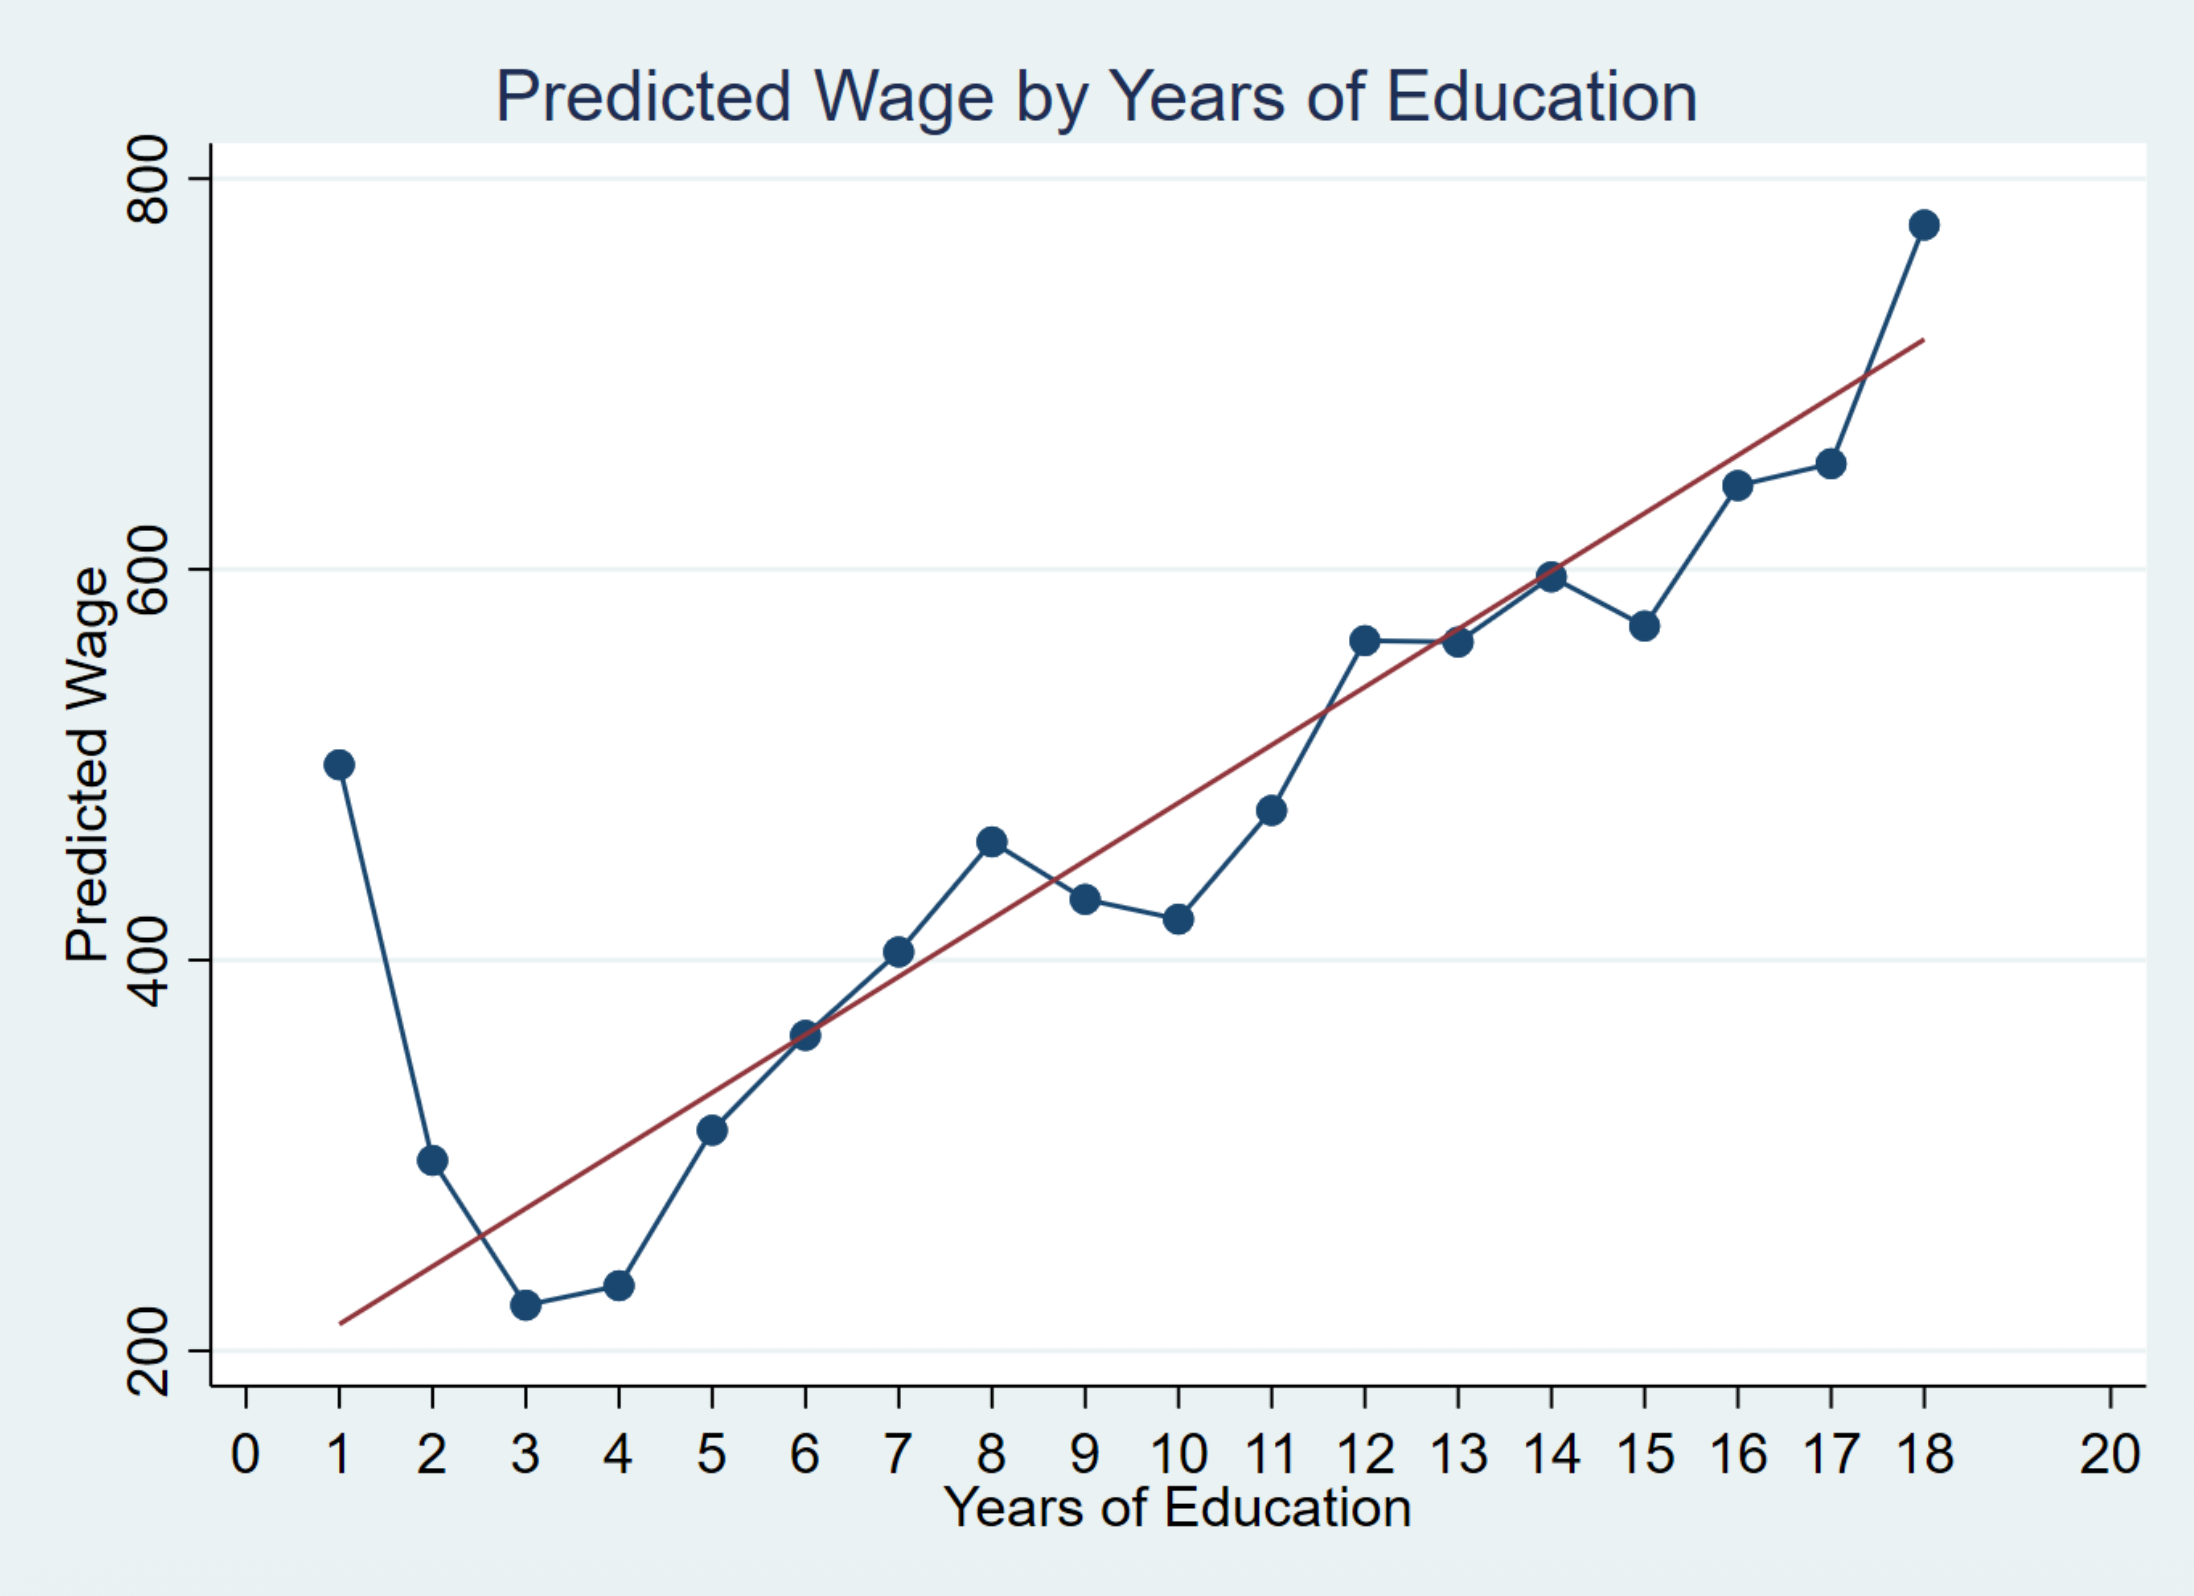
\includegraphics[width=0.78\textwidth]{images/1-22-1}
\end{figure}

There is a small sample problem for years of education less than 8. We trade off variance at this low end, getting a higher bias.

\begin{definition}[Best Linear Predictor]
	The best linear predictor of $y$ given $x$ is defined by
	\[
		\beta=\E\left[xx'\right]^{-1}\E\left[xy\right],
	\]
	where the FOC implies $\E\left[xy\right]=\E\left[xx'\right]\beta$. In order for these equations to have a unique solution, $\E\left[xx'\right]$ must be full rank/invertible. This is equivalent to there being no perfect multicollinearity in $x$; i.e., there is no $a\in \R^k\setminus \{0\}$ such that $x'a = 0$ with probability $1$.
\end{definition}

\section{OLS Estimation}

\begin{remark}	Given a sample $\{y_i,x_i\}_{i=1}^n$, we can apply the sample analogue principle\footnote{Now, $\theta(f)$ is defined as an $\argmin$ of an objective function. We find $\theta(\hat{f})$ now.} and solve the analogous in-sample problem:
	\[
		\min_{b\in\R^k}\frac{1}{n}\sum_{i=1}^n\left(y_i-x_i'b\right)^2
	\]
	to yield an estimator of $\beta$.\boxednote{The solution is $\hat{\beta} = (\frac{1}{n} \sum_i X_iX_i')^{-1} \frac{1}{n} \sum_i X_i Y_i$.} The first order conditions with respect to each $b_j$ imply that at the solution\boxednote{We think of a matrix of $x$ with the rows as observations $1:n$ and the columns as dimensions of $x$ from $1:k$. The first column will be $\vec 1$. Basically, we attach a $1$ to the meaningful characteristics of $x_i$ to get the intercept $\beta_0$ when multiplying by $X$. For example, if we want to consider predicting house price with number of bedrooms, a house would be represented by $(x_i;ly_i) = (1, \text{rooms}; \text{price})$. We want to allow the prediction line to not pass through the origin so the $\beta$s are interpretable as partial covariances.}:
	\[
		-2\cdot\frac{1}{n}\sum_{i=1}^n x_{ij}\left(y_i-x_i'\hat\beta\right)=0\quad\text{for all }1\le j\le k.
	\]

	Stacking these first order conditions gives
	\[
		\begin{pmatrix}
			\frac{1}{n}\sum_{i=1}^n x_{i1}(y_i-x_i'\hat\beta) \\
			\vdots                                            \\
			\frac{1}{n}\sum_{i=1}^n x_{ik}(y_i-x_i'\hat\beta)
		\end{pmatrix}
		=
		\frac{1}{n}\sum_{i=1}^n x_i(y_i-x_i'\hat\beta)=0.
	\]

	Adding $\left( \frac{1}{n} \sum_i x_i x_i' \right)\hat{\beta}$, we get that the FOCs imply
	\[
		\frac{1}{n}\sum_{i=1}^n x_iy_i=\left(\frac{1}{n}\sum_{i=1}^n x_ix_i'\right)\hat\beta.
	\]
	Provided $\frac{1}{n}\sum_{i=1}^n x_ix_i'$ is invertible, which occurs iff none of the columns $x_{\cdot j}$ are collinear, we obtain\boxednote{We can think of $(X_i,Y_i) \in \R^{k+1}$ so our estimator is an object in $\R^{k}$.}
	\[
		\hat\beta=\left(\frac{1}{n}\sum_{i=1}^n x_ix_i'\right)^{-1}\frac{1}{n}\sum_{i=1}^n x_iy_i.
	\]
\end{remark}

\begin{definition}[Fitted Values and Residuals]
	The $i$-th fitted value is:
	\[
		\hat y_i=x_i'\hat\beta.
	\]
	The $i$-th residual is
	\[
		\hat u_i=y_i-\hat y_i.
	\]
\end{definition}

\begin{remark}[FOC of OLS]
	The first order condition of the least squares minimization problem implies
	\[
		\sum_{i=1}^n x_i(y_i-x_i'\hat\beta)=\sum_{i=1}^n x_i\hat u_i=0.
	\]
	We can write this compactly as $X'\hat{u} = 0$.
\end{remark}

\begin{example}[Simple Linear Regression]
	Consider the simple linear model:
	\[
		y=\beta_0+\beta_1x_1+u,
	\]
	where now $x=(1,x_1)'$, and $\beta=(\beta_0,\beta_1)'$. Our earlier work implies\boxednote{Note that this expression for $\beta$ holds regardless of the dimension of $X$.}
	\[
		\beta=\E\left[xx'\right]^{-1}\E\left[xy\right].
	\]
	We have
	\begin{align*}
		\E\left[xx'\right]^{-1}
		&=\begin{pmatrix}
			1   & x_1   \\
			x_1 & x_1^2
		\end{pmatrix}^{-1}
		=\frac{1}{\E\left[x_1^2\right]-\E\left[x_1\right]^2}\begin{pmatrix}
			\E\left[x_1^2\right] & -x_1 \\
			-x_1                 & 1
		\end{pmatrix}, \\
		\E\left[xy\right]
		&=\begin{pmatrix}
			\E\left[y\right] \\
			\E\left[x_1y\right]
		\end{pmatrix}.
	\end{align*}
	It follows that\boxednote{\texthl{apparently this was done in the hw??}}
	\[
		\beta=\frac{1}{\operatorname{Var}(x_1)}\cdot\begin{pmatrix}
			\E\left[x_1^2\right] & -\E\left[x_1\right] \\
			-\E\left[x_1\right]  & 1
		\end{pmatrix}\begin{pmatrix}
			\E\left[y\right] \\
			\E\left[x_1y\right]
		\end{pmatrix}
		=\begin{pmatrix}
			\E\left[y\right]-\beta_1\E\left[x_1\right] \\
			\frac{\operatorname{Cov}(y,x_1)}{\operatorname{Var}(x_1)}
		\end{pmatrix}.
	\]
\end{example}

\begin{remark}[Slope Parameter and Correlation]
	Notice that
	\[
		\beta_1=\frac{\operatorname{Cov}(W,S)}{\operatorname{Var}(S)}=\sqrt{\frac{\operatorname{Var}(W)}{\operatorname{Var}(S)}}\cdot\operatorname{Corr}(W,S),
	\]
	so the slope coefficient is proportional to the correlation between wages and education (likely $>0$).

	Notice that increasing $\operatorname{Var}(W)$ stretches the scatter plot vertically (but leaves the correlation unchanged). The slope coefficient should increase in magnitude.

	Increasing $\operatorname{Var}(S)$ stretches the scatter plot horizontally (but leaves the correlation unchanged). The slope coefficient should decrease in magnitude.
\end{remark}

\begin{example}[Changing units of measurement]
	Suppose wages are now measured in cents per hour rather than dollars per hour. Let $\tilde W$ denote wages in cents:
	\[
		\tilde W=100W.
	\]
	Find the best linear predictor of $\tilde W$ given $S$, i.e. find $(\alpha_0,\alpha_1)$ such that\boxednote{\texthl{ why is including the condition on the expectation of $SU$, $U$ and finding the best linear predictor equivalent to the minimization problem without the error term?}}
	\[
		\tilde W=\alpha_0+\alpha_1S+U;\qquad \E\left[SU\right]=\E\left[U\right]=0.
	\]
	Find that
	\[
		\alpha_1=\frac{\operatorname{Cov}(\tilde W,S)}{\operatorname{Var}(S)}=\frac{100\operatorname{Cov}(W,S)}{\operatorname{Var}(S)}=100\beta_1,
	\]
	\[
		\alpha_0=\E\left[\tilde W\right]-\alpha_1\E\left[S\right]=100(\E\left[W\right]-\beta_1\E\left[S\right])=100\beta_0.
	\]
\end{example}

\begin{example}[Simple Linear Regression Estimation]
	Write the model for each individual $i=1,\ldots,n$ in the sample:
	\[
		y_i=\beta_0+\beta_1x_{i1}+u_i,
	\]
	and estimate the parameters using ordinary least squares:
	\[
		\hat\beta=\left(\frac{1}{n}\sum_{i=1}^n x_ix_i'\right)^{-1}\frac{1}{n}\sum_{i=1}^n x_iy_i
		=\begin{pmatrix}
			\bar y_n-\hat\beta_1\bar x_{1,n} \\
			\frac{\frac{1}{n}\sum_{i=1}^n x_{i1}y_i-\bar x_{1,n}\cdot\bar y_n}{\frac{1}{n}\sum_{i=1}^n x_{i1}^2-(\bar x_{1,n})^2}
		\end{pmatrix}.
	\]
\end{example}

\section{Matrix Notation and Projection}

\begin{remark}[Matrix Notation]
	First write the model for each observation $i=1,\ldots,n$:
	\[
		y_i=x_i'\beta+u_i.
	\]
	Stack the observations into matrices:
	\[
		\begin{pmatrix}
			y_1    \\
			y_2    \\
			\vdots \\
			y_n
		\end{pmatrix}
		=
		\underbrace{\begin{pmatrix}
			-x_1'- \\
			-x_2'- \\
			\vdots \\
			-x_n'-
		\end{pmatrix}}_{\text{design matrix}}
		\beta
		+
		\begin{pmatrix}
			u_1    \\
			u_2    \\
			\vdots \\
			u_n
		\end{pmatrix}.
	\]
	Therefore
	\[
		Y=X\beta+U,
	\]
	where the matrix $X$ is called the design matrix, with columns $X_1,\ldots,X_k\in\R^n$. If we have an intercept, then the first feature $X_1$ is a column of $1$s.

	The least squares minimization problem is
	\[
		\min_{b\in\R^k}\sum_{i=1}^n(y_i-x_i'b)^2\equiv\min_{b\in\R^k}(Y-Xb)'(Y-Xb) = \min_{B \in \R^k} \|Y - Xb\|^2
	\]
	because the sum of squares is just the inner product of $Y-Xb$ with itself.
	To see this, write \[
		\R^n \ni Y - Xb = \begin{bmatrix}
		y_1-x_1'b \\
		\vdots \\
		y_n - x_n'b
		\end{bmatrix} 
	,\] so \[
	\left( Y-Xb \right)'(Y-Xb) = \sum\limits_{i=1}^{n} \left( y_i - x_i'b \right)^2
	.\] Hence, we want to pick $b$ to minimize the distance from $Xb \in \operatorname{Span}(X)$ to $Y\in \R^n$ in the Euclidean norm. This is the point that is the orthogonal projection of $Y$ onto $\operatorname{Span}(X)$.

	We can expand the objective function as
	\[
		(Y-Xb)'(Y-Xb)=Y'Y-Y'Xb-b'X'Y+b'X'Xb=Y'Y-2Y'Xb+b'X'Xb,
	\]
	so the first order condition with respect to $b_j$ is
	\[
		-2\sum_{i=1}^n y_i\cdot x_{ij}+2\sum_{i=1}^n x_{ij}\cdot x_i'\hat\beta=0.
	\]
	Stack the first order conditions into a $k\times 1$ vector:
	\[
		-2\sum_{i=1}^n y_i\cdot x_i+2\left[\sum_{i=1}^n x_ix_i'\right]\hat\beta=0;\quad\text{or}\quad
		-2X'Y+2X'X\hat\beta=0.
	\]
	This yields $X'\left( Y- X\hat{\beta} \right) = 0$,\footnote{This says that every column of $X$ (row of $X'$) is orthogonal to the residual (row).} which is equivalent to (provided $X$ is full column rank):
	\[
		\hat\beta=(X'X)^{-1}X'Y.
	\]
\end{remark}

\begin{remark}	We have used the fact that
	\[
		\sum_{i=1}^n x_ix_i'=X'X,\qquad
		\sum_{i=1}^n y_ix_i=X'Y.
	\]
	To see why these identities hold, consider $X \in \R^{n\times k}$ and $X' \in \R^{k\times n}$, so \[
		X'X = \begin{bmatrix}
			\sum\limits_{i=1}^{n} x_{i_1}^2 & \sum\limits_{i=1}^{n} x_{i 1} x_{i 2} & \cdots \\
		\sum\limits_{i=1}^{n} x_{i 2}x_{i 1} & \sum\limits_{i=1}^{n} x_{i 2}^2 & \cdots \\
		\vdots & & \ddots
		\end{bmatrix} = \sum\limits_{i=1}^{n} X_i X_i'
	.\] Switching a transpose between matrices and vectors moves the transpose.

	The vector of fitted values is $\hat Y=X\hat\beta$, and the vector of residuals is $\hat U=Y-\hat Y$. The FOC of the least squares problem is equivalently written as $X'\hat U=0$. These are the normal equations.
\end{remark}

\begin{proposition}	$(X'X)^{-1}$ exists iff $X$ is full column rank.

	If $X$ is not full column rank, there exists $c\neq 0$ such that $Xc=0$, so $X'Xc=0$, implying $X'X$ is not invertible.

	If $X'X$ is not invertible, there exists $a\neq 0$ such that $X'Xa=0$, so $a'X'Xa=0$. But
	\[
		a'X'Xa=[Xa]'(Xa),
	\]
	which is a sum of squares which equals zero iff $Xa=0$. Since $a\neq 0$, $X$ is not full rank.

	In a simple linear regression, need there to be some variation in $\left( X_i \right)_{1:n}$ so it isn't collinear with the constant. Equivalently, need $\det(X'X)=(n-1)\cdot\widehat{\operatorname{Var}}(x)\neq 0$. When $X_i \in R^2$ with a column of $1$s, then we require that the 2nd column of $X$ is not identically some constant.
\end{proposition}

\begin{theorem}[Projection Theorem]
	Let $y\in\R^n$ and let $S$ be any nonempty subspace of $\R^n$ equipped with the dot product. There exists a unique point $\hat y$ such that $\|y-\hat y\|$ is minimized over $S$.\boxednote{Here, we are thinking of $S$ as a $k$-dimensional subspace of $\R^n$ --- the subset of $\R^n$ spanned by the columns of $X$.} A necessary and sufficient condition for $\hat y$ is that $\hat{y} \in S$ and $\hat y-y$ is orthogonal to every vector in $S$.

	By definition of $\hat\beta$, the vector $X\hat\beta$ is the closest (in the Euclidean norm) to $Y$ in the set of all vectors
	\[
		\{Xb:b\in\R^k\}=S(X),
	\]
	where $S(X)$ denotes the span of the columns of $X$. Given a vector $Y\in\R^n$ and a matrix $X\in\R^{n\times k}$, the projection of $Y$ onto $S(X)$ is the vector\footnote{We previously found $v^* = X\hat{\beta}$.}
	\[
		v^*\in\argmin_{v\in S(X)}\|Y-v\|^2.	
	\]

	While the coefficients $\hat{\beta}$ may not be unique (if $X$ is not full column rank), this theorem guarantees that $X\hat{\beta}$ is unique. 
\end{theorem}

\begin{example}	We can draw the following to provide intuition. Consider $n=2$, $k=2$, and a model with no intercept, so $y_i = \beta x_i + u_i$. Suppose $X = \begin{pmatrix}
	x_1 \\
	x_2
	\end{pmatrix} = \begin{pmatrix}
	1 \\
	0
	\end{pmatrix} $ and $Y = \begin{pmatrix}
	3 \\
	3
	\end{pmatrix} $.

	In this case, $S(X) = \{c \begin{pmatrix}
	1 \\
	0
	\end{pmatrix} : c\in \R\}$, so \[\hat{Y} = P_X Y = \begin{pmatrix}
	3 \\
	0
	\end{pmatrix}, \quad\hat{U} = \begin{pmatrix}
	0 \\
	3
\end{pmatrix}.\]

	We note that $P_X Y$ is the closest point to $Y$ in $S(X)$, while $\hat{U}$ is orthogonal to $S(X)$.
\end{example}


\begin{remark}	Restricting the minimizer to vectors in $S(X)$, the necessary and sufficient condition for the minimizer is
	\[
		x'(Y-\hat Y)=0
	\]
	for all $x\in S(X)$. Since the columns of $X$ are a basis of $S(X)$, this condition is equivalent to
	\[
		X'(Y-\hat Y)=0.
	\]
	$\hat Y\in S(X)$ means $\hat Y=Xb$ for some $b\in\R^k$. Thus
	\[
		X'Y=X'Xb\implies b=(X'X)^{-1}X'Y\implies\hat Y=X(X'X)^{-1}X'Y.
	\]
	That is, the projection of $Y$ onto $S(X)$ is given by $\hat Y=P_XY$, where $P_X$ is the projection matrix defined below.
\end{remark}

\begin{definition}[Projection Matrix]
	Since $X\hat\beta=X(X'X)^{-1}X'Y$, we call $P_X=X(X'X)^{-1}X'$ the projection matrix (it projects $Y$).

	The projection matrix is symmetric:
	\[
		P_X'=[X(X'X)^{-1}X']'=X[(X'X)^{-1}]'=X[(X'X)']^{-1}X'=P_X.
	\]
\end{definition}

\begin{remark}	$P_X$ is also idempotent (meaning $P_X\cdot P_X=P_X$), since:
	\[
		P_XP_X=X(X'X)^{-1}X'X(X'X)^{-1}X'=X(X'X)^{-1}X'=P_X,
	\]
	which reflects the fact that after a vector has been projected on to the span of the columns of $X$, it does not change as a result of the second projection. This is because the projected vector is already a linear combination of the columns of $X$.
\end{remark}

\begin{definition}[Residual Maker Matrix]
	The residual of the projection of $Y$ onto the columns of $X$ is
	\[
		Y-\hat Y=Y-P_XY=(I_n-X(X'X)^{-1}X')Y.
	\]
	Therefore, the matrix $M_X:=I_n-X(X'X)^{-1}X' = I_n - P_X$ is called the residual maker.

	$M_XY$ is the residual of the projection of $Y$ onto the space spanned by the columns of $X$.
\end{definition}

\begin{proposition}[Properties of Residual Maker]
	$M_X$ projects a vector onto the $n-k$ dimensional vector space orthogonal to the column space of $X$. This is called the orthogonal complement of $S(X)$.

	The residual of the projection $M_X y$ is $y - M_X y = P_X y \in S(X) \perp OC(S(X))$.

	Some properties:
	\begin{itemize}
		\item $P_XM_X=M_XP_X=0$, since $P_X(I-P_X)=P_X-P_XP_X=0$.
		\item $P_XX=X(X'X)^{-1}X'X=X$: Projecting $X$ onto its own span does nothing.
		\item $M_XX=X-P_XX=0$: Residual of projecting $X$ onto its own span is $0$.
		\item For any vector $y$, $y=P_Xy+M_Xy=\hat y+\hat u$.
	\end{itemize}
\end{proposition}

\section{$R^2$ and Goodness of Fit}

\begin{definition}[$R^2$]
	\begin{itemize}
		\item $\sum_{i=1}^n(y_i-\bar y)^2:=\text{TSS}$ is called the total sum of squares.
		\item $\sum_{i=1}^n(y_i-x_i'\hat\beta)^2:=\text{SSR}$ is the sum of squared residuals.
		\item $\sum_{i=1}^n(\hat y_i-\bar y)^2:=\text{ESS}$ is the explained sum of squares.
	\end{itemize}
	The coefficient of determination ($R^2$) is given by
	\[
		R^2=\frac{\text{ESS}}{\text{TSS}}.
	\]
\end{definition}

\begin{remark}	Immediately, we see that $SSR \le TSS$ because the $SSR$ is the residuals from letting our line of fit to have a free intercept and slope, while $TSS$ fixes a slope of $0$.
	$R^2$ measures how well OLS estimation of a linear model which includes a constant as a regressor fits a given dataset relative to a model only containing a constant. In other words, we are comparing two models:
	\begin{enumerate}[label=(\roman*)]
		\item $y = \beta_0 + u$, which implies $\hat{\beta}0^{OLS} = \overline{y}$
		\item $y = \beta_0 + \beta_1 x + \epsilon$,
	\end{enumerate}
	and seeing what fraction the SSR of the second model is of the SSR of the first model.
	

	We have:
	\[
		R^2=\frac{\text{ESS}}{\text{TSS}}=\frac{\sum_{i=1}^n(\hat y_i-\bar y_n)^2}{\sum_{i=1}^n(y_i-\bar y_n)^2}=1-\frac{\sum_{i=1}^n(y_i-x_i'\hat\beta)^2}{\sum_{i=1}^n(y_i-\bar y_n)^2},
	\]
	where the third equality follows from $SSR + ESS = TSS$ (shown later).

	The second and third equalities imply $0\le R^2\le 1$.

	$R^2=1$ iff $\text{SSR}=0$, which means $\hat U=0$.

	$R^2=0$ iff $\text{SSR}=\text{TSS}$, which implies all $y_i$ are identical and $\hat\beta=(\bar y,0,\ldots,0)$ provided $X$ is full column rank. In this case the model fits the data no better than a constant would; knowing $x$ does not help us predict $y$.
\end{remark}

\begin{proof} (Decomposition of $R^2$)
	Let $P_c=\mathbf{1}(\mathbf{1}'\mathbf{1})^{-1}\mathbf{1}'=\frac{1}{n}\mathbf{1}\mathbf{1}'$ be the projection matrix onto the span of the column vector of ones in $\R^n$. Then $P_cY=\frac{1}{n}\mathbf{1}\mathbf{1}'Y=\bar y_n\mathbf{1}$, so:
	\begin{align*}
		\text{TSS}&=\|Y-P_cY\|^2=\|M_cY\|^2 \\
		\text{ESS}&=\|P_XY-P_cY\|^2=\|P_XY-P_XP_cY\|^2=\|P_XM_cY\|^2 \\
		\text{SSR}&=\|Y-P_XY\|^2=\|M_XY\|^2=\|M_XM_cY\|^2.
	\end{align*}\boxednote{We see that \begin{align*}
		M_X M_c Y &= M_X Y - M_X P_c Y \\
		           &= M_X Y,
	\end{align*}since $P_c Y\in S(X)$ means $M_X P_c Y=0$.}

	Finally, since $P_XM_cY \in S(X)$ and $M_XM_cY \in OC(S(X))$ are orthogonal:
	\[
		\|M_XM_cY\|^2+\|P_XM_cY\|^2=\|M_XM_cY+P_XM_cY\|^2=\|M_cY\|^2,
	\]
	so $\text{ESS}+\text{SSR}=\text{TSS}$. This shows that
	\[
		R^2=\frac{\text{ESS}}{\text{TSS}}=1-\frac{\text{SSR}}{\text{TSS}}.
	\]
\end{proof}

\begin{remark}	High $R^2$ does not mean the linear model is ``correct'' in the sense that it provides a causal explanation of the relationship between $x$ and $y$.

	On the other hand, low $R^2$ does not preclude a causal relationship between $x$ and $y$ in a linear model.

	$R^2$ is an estimator of the population $R^2$, defined by
	\[
		R^2_{\text{pop}}=1-\frac{\operatorname{Var}(u)}{\operatorname{Var}(y)},
	\]
	since $\text{SSR}/n$ is an estimate of $\operatorname{Var}(u)$ and $\text{TSS}/n$ is an estimate of $\operatorname{Var}(y)$.

	Decomposing variance in $y$ as
	\[
		\operatorname{Var}(y):=\E\left[\operatorname{Var}(y\mid x)\right]+\operatorname{Var}(\E\left[y\mid x\right]).
	,\]
	the first term represents the unexplained variation in $y$\footnote{Since $\operatorname{Var}\left(y \mid x\right) = \E\left[\left( y - \E\left[y\mid x\right]  \right)^2\right]$ is the square of expected residual against the best linear predictor.}, while the second term represents variation in $y$ that is explained by the model.
\end{remark}

\begin{remark}	Note that SSR always weakly decreases when a regressor is added to the model.

	Suppose we estimate the intercept and slope parameters in the following models by OLS:
	\[
		A:y_i=\alpha_0+\alpha_1x_{i1}+u_i;\qquad
		B:y_i=\beta_0+\beta_1x_{i1}+\beta_2x_{i2}+v_i.
	\]
	Let $\text{SSR}_A$ be the SSR resulting from OLS estimation of $A$, and $\text{SSR}_B$ be the SSR resulting from OLS estimation of $B$.

	We have
	\[
		\text{SSR}_A=\min_{a_0,a_1}\sum_{i=1}^n(y_i-a_0-a_1x_{i1})^2=\sum_{i=1}^n(y_i-\hat\alpha_0-\hat\alpha_1x_{i1})^2;
	\]
	\[
		\text{SSR}_B=\min_{b_0,b_1,b_2}\sum_{i=1}^n(y_i-b_0-b_1x_{i1}-b_2x_{i2})^2=\sum_{i=1}^n(y_i-\hat\beta_0-\hat\beta_1x_{i1}-\hat\beta_2x_{i2})^2.
	\]

	$\text{SSR}_B\le\text{SSR}_A$: after finding $(\hat\alpha_0,\hat\alpha_1)$, setting $(b_0,b_1,b_2)=(\hat\alpha_0,\hat\alpha_1,0)$ is always feasible. In general, the optimal $b_2\ne0$, so adding $x_2$ strictly reduces SSR.

	This also means $R^2$ increases when adding regressors, because
	\[
		R^2_A=1-\frac{\text{SSR}_A}{\text{TSS}}\le 1-\frac{\text{SSR}_B}{\text{TSS}}=R^2_B.
	\]
\end{remark}

\begin{definition}[Adjusted $R^2$]
	Adjusted $R^2$ penalizes additional regressors, and is defined by
	\[
		\bar R^2=1-\frac{n-1}{n-k-1}\frac{\text{SSR}}{\text{TSS}}=1-\frac{n-1}{n-k-1}(1-R^2)\le R^2
	,\]
	where $k$ is the number of regressors (excluding the intercept) and $n$ is the sample size.
\end{definition}

\section{Finite Sample Properties of OLS}

Economists don't care too much about $R^2$ because it's a measure of prediction accuracy, not causality.

\begin{remark}[Gauss Markov Assumptions]
	We will work with the following assumptions to provide an ideal setting for linear regression, then derive the expectation and variance of OLS estimators:
	\begin{itemize}
		\item MLR.1: The model under consideration is
		      \[y=\beta_0+\beta_1x_1+\cdots+\beta_kx_k+u\equiv x'\beta+u.\]
		      \boxednote{By itself, MLR.1 imposes no restriction on $x$ because we can put $u = y - x'\beta$ and always represent $y$ in this way.}
		\item MLR.2: We observe an iid sample of $\{y_i,x_i\}_{i=1}^n$.
		\item MLR.3: There is no perfect collinearity in the sample (so $\left( X'X \right)^{-1}$ exists with probability $1$ and a unique $\hat\beta$ exists).
		\item MLR.4: $\E\left[u\mid x\right]=0$.\footnote{Hence, $\E\left[y \mid x\right] $ is a linear function of $x$.}
		\item MLR.5: (Homoskedasticity) $\operatorname{Var}(y\mid x)=\sigma^2$.\footnote{There is generally no good reason to believe in homoskedasticity. Correcting for heteroskedasticity would weight sample points where the error variance is lower, since these points give more information on the relationship between $y$ and $x$. This leads to generalized OLS, which is not used often because a heteroskedasticity correction is difficult (the standard deviation of the error as a function of $x$ is not known).}
	\end{itemize}
	MLR stands for multiple linear regression.
\end{remark}

\begin{proposition}	Suppose MLR.1--MLR.4 hold. By $\E\left[u\mid x\right] =0$ and since $(u_i,x_i)$ is independent of $x_j$ for $j\neq i$, we obtain for each $i$:
	\[
		0=\E\left[u_i\mid x_i\right]=\E\left[u_i\mid x_1,\ldots,x_n\right].
	\]
	This is equivalently written as
	\[
		\E\left[U\mid X\right]=0.
	\]
	This is in turn equivalent to
	\[
		\E\left[Y\mid X\right]=X\beta.
	\]
\end{proposition}
\begin{proof}
	(Bias.) It follows that
	\begin{align*}
		\E\left[\hat\beta\mid X\right]
		&=\E\left[(X'X)^{-1}X'Y\mid X\right]=(X'X)^{-1}X'\E\left[Y\mid X\right] \\
		&=(X'X)^{-1}X'X\beta=\beta.
	\end{align*}
	By the Law of Iterated Expectation:
	\[
		\E\left[\hat\beta\right]=\E\left[\E\left[\hat\beta\mid X\right]\right]=\beta,
	\]
	so $\hat\beta$ is unbiased.

	(Variance.) Suppose in addition that $\operatorname{Var}(u_i\mid x_i)=\sigma^2$. (MLR.5)

	Since the error variance does not depend on the value of $x_i$, it is called homoskedastic. If the error variance depends on $x_i$, $u_i$ is heteroskedastic and MLR.5 fails.

	Under homoskedasticity,
	\[
		\operatorname{Var}(U\mid X)=\sigma^2I_n.
	\]
	To see this, note that the $(i,j)$ entry is given by
	\[
		\operatorname{Var}(U\mid X)_{i,j}=\E\left[UU'\mid X\right]_{i,j}=\E\left[u_iu_j\mid X\right]=
		\begin{cases}
			\E\left[u_i^2\mid x_i\right]      & i=j      \\
			\E\left[u_iu_j\mid x_i,x_j\right] & i\neq j.
		\end{cases}
	\]

	We have $\E\left[u_i^2\mid x_i\right]=\sigma^2$ because
	\[
		\E\left[u_i^2\mid x_i\right]-\underbrace{(\E\left[u_i\mid x_i\right])^2}_{=0}=\operatorname{Var}(u_i\mid x_i)=\sigma^2.
	\]
	We also have that for $i\ne j$,
	\[
		\E\left[u_iu_j\mid x_i,x_j\right]=\E\left[u_i\E\left[u_j\mid u_i,x_i,x_j\right]\mid x_i,x_j\right]=\E\left[u_i\E\left[u_j\mid x_j\right]\mid x_i,x_j\right]=0.
	\] The off diagonal elements are $0$ because of MLR.2,\footnote{MK: and because of MLR.4, I think.} \emph{not} because of MLR.5.

	Under heteroskedasticity, the off diagonal elements are still $0$ but\[\E[u_i^2\mid x_i]=f(x_i),\]so
	\[
		\operatorname{Var}(U\mid X)=
		\begin{pmatrix}
			f(x_1) & 0      & 0      & 0      \\
			0      & f(x_2) & 0      & 0      \\
			0      & 0      & \ddots & 0      \\
			0      & 0      & 0      & f(x_n)
		\end{pmatrix} =: \Omega
		.\]

	We now conclude that (*)
	\[
		\operatorname{Var}(\hat\beta\mid X)=\operatorname{Var}(\beta+(X'X)^{-1}X'U\mid X)=(X'X)^{-1}X'\Omega X(X'X)^{-1}.
	\]
	Under homoskedasticity, $\Omega=\sigma^2I_n$, and so the variance becomes
	\[
		\operatorname{Var}(\hat\beta\mid X)=\sigma^2(X'X)^{-1}X'I_nX(X'X)^{-1}=\sigma^2(X'X)^{-1}.
	\]

	(*) follows from $\hat{\beta} = \beta + \left( \underbrace{\left( X'X \right)^{-1}X'}_{A(X)} U \mid X \right)$, so \[
		\operatorname{Var}\left(\left( \hat{\beta} \mid X \right)\right)= A(X) \operatorname{Var}\left(U \mid X\right) A(X)' = \sigma^2 \left( X'X \right)^{-1}
	,\] where the last equality follows from MLR.5.
\end{proof}

\begin{theorem}[Gauss-Markov Theorem]
	Under MLR.1--5, the OLS estimator is the ``best linear unbiased estimator'', which means it has the ``smallest'' variance in the class of linear estimators that are also unbiased conditional on $X$. This result is known as the Gauss-Markov Theorem.

	Our goal is to show that
	\[
		\operatorname{Var}(\hat\beta\mid X)=\sigma^2(X'X)^{-1}
	\]
	is ``smaller'' than the conditional variance of any other estimator $\tilde\beta=A(X)Y$ which also satisfies $\E\left[\tilde\beta\mid X\right]=\beta$. Precisely: $\operatorname{Var}(\tilde\beta\mid X)-\operatorname{Var}(\hat\beta\mid X)=D$ is a positive-semidefinite matrix.
\end{theorem}

\begin{remark}	In particular, let $r$ be a $k\times 1$ vector, and let $r'\beta$ denote a linear combination of the $\beta_j$. The Gauss-Markov theorem implies that $r'\hat\beta$ is the Best Linear Unbiased Estimator of $r'\beta$, since
	\[
		\operatorname{Var}(r'\tilde\beta\mid X)-\operatorname{Var}(r'\hat\beta\mid X)=r'\operatorname{Var}(\tilde\beta\mid X)r-r'\operatorname{Var}(\hat\beta\mid X)r=r'Dr\ge 0.
	\]
	For example, if $r=(0,0\ldots,0,\underbrace{1}_{\text{$j$-th position}},0,\ldots,0)$, then $r'\hat\beta=\hat\beta_j$, and so $\operatorname{Var}(\hat\beta_j\mid X)\le\operatorname{Var}(\tilde\beta_j\mid X)$.
\end{remark}

\begin{proof}(Gauss-Markov Theorem)
	Now consider any other linear unbiased (conditional on $X$) estimator of $\beta$ defined by \[
		\tilde{\beta} = A(X) Y
	.\] Recall that $\hat{\beta} = A(X) = \left( X'X \right)^{-1}X'$. Note that 
	\begin{align*}
		\E\left[\tilde{\beta} \mid X\right]  &= \E\left[A(X) Y \mid X\right]  \\
		&= A(X) \E\left[Y \mid X\right]  \\
		&= A(X) X \beta
	,\end{align*}
	which must be equal to $\beta$ for any $\beta \in \R^k$ if $\tilde{\beta}$ is unbiased. In this case, for any $\beta \in \R^k$, \[
		\left( A(X) X - I_k \right)\beta = 0
	,\] so \[
		A(X)X = I_k
	.\] 
	Therefore, if we require $\hat{\beta}$ to be unbiased, we require $A(X) X = I_k$. Note that $A(X)$ as defined in OLS satisfies this.

	From now on, write $A := A\left( X \right)$.

	Next, we compute the variance of $\tilde{\beta} = AY$ conditional on $X$:
	\[
		\operatorname{Var}\left(\tilde{\beta} \mid X\right) = \operatorname{Var}(AY\mid X)=A\operatorname{Var}(Y\mid X)A'=A\operatorname{Var}(U\mid X)A'=\sigma^2AA'.
	\]
	If $A=(X'X)^{-1}X'$, we obtain the OLS estimator, with variance $\sigma^2(X'X)^{-1}$.

	We really want to show that $\operatorname{Var}\left(\tilde{\beta}\mid X\right) \ge \operatorname{Var}\left(\hat{\beta} \mid X\right)$. But how should we define an ordering of matrices? One way is to say that the first matrix is larger if the difference of the first minus the second is positive semidefinite. This is because taking a linear combination of the $\hat{\beta}$ estimate's components with a vector $r$ multiplies the variance by $r$ and $r'$ on either side, respectively.

	Define $C = A - (X'X)^{-1}X'$, so that $A = C + (X'X)^{-1}X'$. Note that the unbiasedness constraint $AX = I_k$ gives
	\[
		CX = AX - (X'X)^{-1}X'X = I_k - I_k = 0.
	\]
	Expanding $AA'$:
	\begin{align*}
		AA' &= \Bigl(C + (X'X)^{-1}X'\Bigr)\Bigl(C + (X'X)^{-1}X'\Bigr)' \\
		    &= CC' + \underbrace{CX}_{=\,0}(X'X)^{-1} + (X'X)^{-1}\underbrace{(CX)'}_{=\,0} + (X'X)^{-1}X'X(X'X)^{-1} \\
		    &= CC' + (X'X)^{-1}.
	\end{align*}
	Therefore,
	\begin{align*}
		\operatorname{Var}\left(\tilde{\beta} \mid X\right) - \operatorname{Var}\left(\hat{\beta} \mid X\right)
			&= \sigma^2 AA' - \sigma^2(X'X)^{-1} \\
			&= \sigma^2\bigl[CC' + (X'X)^{-1}\bigr] - \sigma^2(X'X)^{-1} \\
			&= \sigma^2 CC'.
	\end{align*}
	Because $CC'$ is always positive semidefinite, we are done.

\end{proof}

\begin{remark}[Why positive semidefiniteness?]
	In particular,
	\begin{align*}
		\operatorname{Var}\left(\left( r' \hat{\beta} \mid X \right)\right) - \operatorname{Var}\left( r' \hat{\beta} \mid X\right) &=  r' \operatorname{Var}\left(\tilde{\beta} \mid X\right)r - r' \operatorname{Var}\left(\hat{\beta} \mid X\right)r \\
		&= r' \left[ \operatorname{Var}\left(\tilde{\beta }\mid X\right) - \operatorname{Var}\left(\hat{\beta} \mid X\right) \right]r \\
		&= \sigma^2 r' C C' r \ge 0
	,\end{align*}
	where the inequality follows from positive semidefiniteness of $C C'$. Therefore $r' \hat{\beta}$ is at least as efficient as $r' \tilde{\beta}$ for estimate $r' \beta$.
	In particular, \[
		\operatorname{Var}\left(\hat{\beta}_j \mid X\right) \le \operatorname{Var}\left( \left( \tilde{\beta}_j \mid X \right)\right)
	\] for any $j$. The OLS estimator $\hat{\beta}$ is efficient in the sense that componentwise, it achieves the lowest variance of an unbiased linear estimator of the conditional mean.\footnote{In fact, OLS is the best unbiased estimator (not restricting to just linear estimators). But doubly in fact, the only unbiased estimators are linear.}
\end{remark}


% Week 4 Slides
\section{Large Sample Properties of OLS}

\begin{assumption}	Now drop the assumptions that $\E\left[u_i \mid x_i\right] = 0$\footnote{i.e. that the relationship between $y$ and $x$ is linear.} and $\operatorname{Var}(u_i \mid x_i) = \sigma^2$ but assume we have an iid sample $\{y_i, x_i\}_{i=1}^n$.
	
	The model is \[
		y = x'\beta + u
	.\] 
	
	Suppose that $\E\left[ux\right] = 0$ and that $\E\left[xx'\right] $ is invertible. Note that $\frac{1}{n} \sum_{i=1}^{n} x_i x_i'$ may not be invertible under these assumptions (which was MLR.3), but it is invertible with probability approaching one because $\E\left[xx'\right] ^{-1}$ exists.
	
	In other words, the population condition that $\E\left[x x'\right]^{-1}$ existing is stronger (as in implies the sample condition) than the sample condition of $\frac{1}{n}\sum_{i=1}^{n} x_i x_i'$ being invertible.\boxednote{This is because if $\E\left[x x'\right] ^{-1}$ exists, the determinant of $\E\left[x x'\right] $ as a continuous function of $x$ is nonzero; convergence in probability gives a neighborhood of invertible matrices for which the determinant is nonzero. By the WLLN/convergence in probability, $\frac{1}{n}\sum x_i x_i'$ is eventually within this ball a.s.}
\end{assumption}

\begin{proposition}[Consistency]
	Under these weaker assumptions, the OLS estimator is consistent.
\end{proposition}
\begin{proof}
	First, note that \[
		\frac{1}{n} \sum_{i=1}^{n} x_i x_i' \xrightarrow{p} \E\left[xx'\right] ; \quad \frac{1}{n} \sum_{i=1}^{n} x_i y_i \xrightarrow{p} \E\left[xy\right] 
	.\] 
	by the law of large numbers, because $\{x_i x_i'\}_{i \ge 1}$ is an iid sequence of random matrices with expectation $\E\left[xx'\right] $, and $\{x_i y_i\}_{i \ge 1}$ is an iid sequence of random vectors with expectation $\E\left[xy\right] $.

	Marginal convergence in probability implies joint convergence in probability: \[
		\left( \frac{1}{n} \sum_{i=1}^{n} x_i x_i', \frac{1}{n} \sum_{i=1}^{n} x_i y_i \right) \xrightarrow{p} \left( \E\left[xx'\right] , \E\left[xy\right]  \right) 
	.\] 
	
	Now let $g(x,y) = x^{-1}y$, where $x^{-1}$ denotes a matrix inverse. $g$ is continuous if $x$ is invertible (matrix version of $x \ne 0$).
	
	It therefore follows by the continuous mapping theorem that \[
		\left( \frac{1}{n} \sum_{i=1}^{n} x_i x_i' \right)^{-1} \frac{1}{n} \sum_{i=1}^{n} x_i y_i \xrightarrow{p} \E\left[xx'\right] ^{-1} \E\left[xy\right] = \beta + \E\left[xx'\right] ^{-1} \E\left[xu\right] = \beta
	\] by plugging in $y = x' \beta + u$. 
\end{proof}

\begin{proposition}[Asymptotic Normality of OLS]
	Assume $\operatorname{Var}(xu)$ exists also. Then because $\E\left[xu\right] = 0 \implies \left( \E\left[xu\right]  \right)^2 = 0$, \[
		\operatorname{Var}(xu) = \E\left[xu(xu)'\right] = \E\left[u^2 xx'\right] 
	.\] 
	
	We have \[
		\sqrt{n} \left( \hat{\beta}_n - \beta \right) \xrightarrow{d} N(0, \Sigma)
	,\] where $\Sigma = \E\left[xx'\right] ^{-1} \operatorname{Var}(xu) \E\left[xx'\right] ^{-1}$.
\end{proposition}

\begin{proof}
	First note that \[
		\sqrt{n} \left( \hat{\beta}_n - \beta \right) = \left( \frac{1}{n} \sum_{i=1}^{n} x_i x_i' \right)^{-1} \frac{1}{\sqrt{n}} \sum_{i=1}^{n} x_i u_i
	.\] 

	Since the sequence of vectors $\left\{ (y_i, x_i')' \right\}_{i \ge 1}$ is iid, the sequence $\{x_i (y_i - x_i' \beta)\}_{i \ge 1}$ is iid. Therefore, the CLT implies:\boxednote{CLT applies:\begin{align*}\tfrac{1}{\sqrt{n}}\sum_i (X_i-\mu)&=\sqrt{n}(\bar X_n-\mu).\end{align*}} \[
		\frac{1}{\sqrt{n}} \sum_{i=1}^{n} x_i u_i \xrightarrow{d} N(0, \operatorname{Var}(xu))
	.\] 
	
	Applying Slutsky's Theorem gives \[
		\left( \frac{1}{n} \sum_{i=1}^{n} x_i x_i' \right)^{-1} \frac{1}{\sqrt{n}} \sum_{i=1}^{n} x_i u_i \xrightarrow{d} N(0, \Sigma)
	,\] as desired.
\end{proof}

\section{Estimation of $\Sigma$}

Deriving asymptotic normality of $\hat{\beta}$ will enable us to conduct hypothesis tests about the unknown parameter $\beta$.

Since we do not know $\Sigma$, we must construct a consistent estimator of it to yield an asymptotic distribution whose quantiles are known so we may conduct tests.

For the time being (the next two propositions), suppose MLR.4 and MLR.5 hold, so we have an easy case in which $\E\left[u \mid x\right] = 0$ and $\operatorname{Var}(u \mid x) = \sigma^2$. Then \[
	\operatorname{Var}(xu) = \E\left[u^2 xx'\right] = \E\left[\E\left[u^2 \mid x\right] xx'\right] = \E\left[\operatorname{Var}\left(u \mid x\right) x x'\right] = \sigma^2 \E\left[xx'\right] 
.\] 

It follows that \[
	\Sigma =  \E\left[x x'\right] ^{-1} \sigma^2  \E\left[x x'\right]  \E\left[x x'\right] ^{-1} = \sigma^2 \E\left[xx'\right] ^{-1}
.\] 


\begin{proposition}[$\hat{\sigma}^2$ is consistent]
	A natural estimator of $\E\left[xx'\right] ^{-1}$ is $\left( \frac{1}{n} \sum_{i=1}^{n} x_i x_i' \right)^{-1}$.\boxednote{The degree of freedom correction $k$ is the number of $\beta_j$s we are estimating. It is the width of the design matrix. Note that the adjusted $R^2$ does not count the intercept in its $k$, but when $k$ is the df correction, it is just always the number of $\beta$s to be estimated.}
	
	It remains to find a consistent estimator of $\sigma^2$. We use \[
		\hat{\sigma}^2 = \frac{1}{n-k} \sum_{i=1}^{n} \hat{u}_i^2 = \frac{\text{SSR}}{n-k}
	.\] 
	
	Next, note that $\hat{U} = M_X Y = M_X (X\beta + U) = M_X U$, so\footnote{The third equality follows from symmetry and idempotency of $M_X$.} \[
		\text{SSR} = \|M_X U\|^2 = U' M_X' M_X U = U' M_X U = U'U - U' P_X U
	.\] 
	Therefore, \[
		\begin{aligned}
			\hat{\sigma}^2
			&= \frac{\operatorname{SSR}}{n-k}
			= \frac{\operatorname{SSR}}{n}\frac{n}{n-k} \\
			&= \frac{n}{n-k} \left( \frac{1}{n} \sum_{i=1}^{n} u_i^2 - \left( \frac{1}{n} \sum_{i=1}^{n} u_i x_i' \right) \left( \frac{1}{n} \sum_{i=1}^{n} x_i x_i' \right)^{-1} \left( \frac{1}{n} \sum_{i=1}^{n} x_i u_i \right) \right) \\
			&\xrightarrow{p} \sigma^2 - 0 \cdot \E\left[xx'\right]^{-1} \cdot 0
			= \sigma^2
		\end{aligned}
	,\] by the continuous mapping theorem.
	
	Another application of the continuous mapping theorem implies that a consistent estimator of $\Sigma$ is given by \[
		\hat{\Sigma} = \hat{\sigma}^2 \left( \frac{1}{n} \sum_{i=1}^{n} x_i x_i' \right)^{-1} \xrightarrow{p} \sigma^2 \E\left[x x'\right]^{-1} = \Sigma
	.\] 
\end{proposition}

\begin{proposition}[$\hat{\sigma}^2$ is unbiased]
	We now show the degrees of freedom correction $n-k$ yields an unbiased estimate of $\sigma^2$. To see this, note that \[
		(n-k) \hat{\sigma}^2 = \text{SSR}
	,\] and
	\[
		\begin{aligned}
			\E\left[\text{SSR} \mid X\right]
			&= \E\left[U'U \mid X\right] - \E\left[U' P_X U \mid X\right] \\
			&= \sum_{i=1}^{n} \E\left[u_i^2 \mid X\right] - \E\left[U' P_X U \mid X\right] \\
			&= n\sigma^2 - \E\left[U' P_X U \mid X\right]
		\end{aligned}
	.\]
	We want to remove $P_X$ from the expectation, but it is in the middle of the product.

	Since expectations can be exchanged with summations, for a random matrix $A$: \[
		\E\left[\operatorname{tr}(A)\right] = \operatorname{tr}(\E\left[A\right] )
	.\] 
	
	The trace has a special property called invariance under cyclic permutations.
	
	For our purposes, this means that for any matrices $A, B$ such that $AB$ and $BA$ are well defined: \[
		\operatorname{tr}(AB) = \operatorname{tr}(BA)
	.\] 
	Since $U' P_X U$ is a scalar, it equals its trace, so \begin{align*}
		\E\left[U' P_X U \mid X\right] &= \E\left[\operatorname{tr}(U' P_X U) \mid X\right] \\ &= \E\left[\operatorname{tr}(P_X U U') \mid X\right] \\
									   &= \operatorname{tr}\left( P_X \E\left[UU' \mid X\right]  \right) \\
									   &= \operatorname{tr}(P_X \sigma^2 I_n) \\ &= \sigma^2 \operatorname{tr}\left( X(X'X)^{-1}X' \right)  \\ &= \sigma^2 \operatorname{tr}\left( X'X (X'X)^{-1} \right) \\ &= \sigma^2 \operatorname{tr}(I_k) \\ &= k\sigma^2
	.\end{align*} 
	
	This implies $\E\left[\text{SSR} \mid X\right] = n\sigma^2 - k\sigma^2 = (n-k)\sigma^2$, so $ \hat{\sigma}^2 = \frac{\E\left[\operatorname{SSR}\mid X\right] }{n-k}$ is an unbiased estimator of $\sigma^2$.
\end{proposition}

\begin{remark}
	If we do not assume $\E\left[u \mid x\right] = 0$ and $\operatorname{Var}(u \mid x) = \sigma^2$, $\Sigma$ does not simplify, and we use \[
		\hat{\Sigma} = \left( \frac{1}{n} \sum_{i=1}^{n} x_i x_i' \right)^{-1} \left( \frac{1}{n} \sum_{i=1}^{n} \hat{u}_i^2 x_i x_i' \right) \left( \frac{1}{n} \sum_{i=1}^{n} x_i x_i' \right)^{-1}
	.\] 
	
	Note that this is identical to $n \cdot (X'X)^{-1} X' \hat{\Omega} X (X'X)^{-1}$, where \[
		\hat{\Omega} = 
		\begin{pmatrix}
			\hat{u}_1^2 & 0 & 0 & 0 \\
			0 & \hat{u}_2^2 & 0 & 0 \\
			0 & 0 & \ddots & 0 \\
			0 & 0 & 0 & \hat{u}_n^2
		\end{pmatrix}
	.\] 

	Proving consistency boils down to showing that \[
		\frac{1}{n} \sum_{i=1}^{n} \hat{u}_i^2 x_i x_i' \xrightarrow{p} \E\left[u^2 xx'\right] 
	.\] 
	
	First, decompose this quantity as \[
		\frac{1}{n} \sum_{i=1}^{n} \hat{u}_i^2 x_i x_i' = \frac{1}{n} \sum_{i=1}^{n} u_i^2 x_i x_i' + \frac{1}{n} \sum_{i=1}^{n} (\hat{u}_i^2 - u_i^2) x_i x_i'
	.\] 

	We have \[
		\frac{1}{n} \sum_{i=1}^{n} u_i^2 x_i x_i' \xrightarrow{p} \E\left[u^2 xx'\right] 
	,\] so it remains to show that \[
		\frac{1}{n} \sum_{i=1}^{n} (\hat{u}_i^2 - u_i^2) x_i x_i' = o_p(1)
	.\] 
	
	We prove that every element of this matrix converges to zero in probability.

	Fix $j,k$ element $\frac{1}{n} \sum_{i=1}^{n} (\hat{u}_i^2 - u_i^2) x_{i,j} x_{i,k}$, and observe that \[
		\begin{aligned}
			\left| \frac{1}{n} \sum_{i=1}^{n} (\hat{u}_i^2 - u_i^2) x_{i,j} x_{i,k} \right|
			&\le \frac{1}{n} \sum_{i=1}^{n} |\hat{u}_i^2 - u_i^2| |x_{i,j} x_{i,k}| \\
			&\le \max_{1 \le i \le n} |\hat{u}_i^2 - u_i^2| \frac{1}{n} \sum_{i=1}^{n} |x_{i,j} x_{i,k}|
		\end{aligned}
	.\] 
	
	Since \[
		\frac{1}{n} \sum_{i=1}^{n} |x_{i,j} x_{i,k}| \xrightarrow{p} \E\left[|x_{i,j} x_{i,k}|\right] 
	,\] it is sufficient to prove \[
		\max_{1 \le i \le n} |\hat{u}_i^2 - u_i^2| \xrightarrow{p} 0
	.\] 

	To this end, note that \[
		\hat{u}_i - u_i = x_i' (\beta - \hat{\beta}_n)
	,\] so since $\hat{u}_i = y_i - x_i' \hat{\beta}_n = x_i' (\beta - \hat{\beta}_n) + u_i$, we have: \[
		\begin{aligned}
			|\hat{u}_i^2 - u_i^2|
			&= |x_i' (\beta - \hat{\beta}_n) (\hat{u}_i + u_i)| \\
			&= |x_i' (\beta - \hat{\beta}_n) (x_i' (\beta - \hat{\beta}_n) + 2u_i)| \\
			&= \left| \left( x_i' (\beta - \hat{\beta}_n) \right)^2 + 2u_i x_i' (\beta - \hat{\beta}_n) \right| \\
			&\le \left| \left( x_i' (\beta - \hat{\beta}_n) \right)^2 \right| + 2 \left| u_i x_i' (\beta - \hat{\beta}_n) \right|
		\end{aligned}
	.\] 

	Next, using the Cauchy-Schwarz inequality, we obtain \[
		\begin{aligned}
			\max_{1 \le i \le n} |\hat{u}_i^2 - u_i^2|
			&\le \|\beta - \hat{\beta}_n\|^2 \max_{1 \le i \le n} \|x_i\|^2 + 2 \|\beta - \hat{\beta}_n\| \max_{1 \le i \le n} \|x_i u_i\| \\
			&= \left\| \sqrt{n} (\beta - \hat{\beta}_n) \right\|^2 \frac{\max_{1 \le i \le n} \|x_i\|^2}{n} \\
			&\quad + 2 \left\| \sqrt{n} (\beta - \hat{\beta}_n) \right\| \frac{\max_{1 \le i \le n} \|x_i u_i\|}{\sqrt{n}}
		\end{aligned}
	.\] 

	Since $\sqrt{n} (\beta - \hat{\beta}_n)$ converges in distribution, we must show: \[
		\frac{\max_{1 \le i \le n} \|x_i\|^2}{n} \xrightarrow{p} 0
		\qquad \text{and} \qquad
		\frac{\max_{1 \le i \le n} \|x_i u_i\|}{\sqrt{n}} \xrightarrow{p} 0
	.\] 
\end{remark}

\begin{lemma}	Let $\{Z_i\}_{i \ge 1}$ be a sequence of identically distributed random vectors such that $\E\left[\|Z_i\|^r\right] < \infty$. Then \[
		\frac{\max_{1 \le i \le n} \|Z_i\|}{n^{1/r}} \xrightarrow{p} 0
	.\] 
\end{lemma}

\begin{proof}
	Fix $\epsilon > 0$ and note that
	\begin{align*}
		\P\left( \max_{1 \le i \le n} \|Z_i\| > \epsilon n^{1/r} \right) &= \P\left( \cup_{i=1}^n \{\|Z_i\|^r > \epsilon^r n\} \right) \\
		&\le \sum_{i=1}^{n} \P\left( \|Z_i\|^r > \epsilon^r n \right) \\
		&= \sum_{i=1}^{n} \P\left( \|Z_i\|^r \mathds{1}(\|Z_i\|^r > \epsilon^r n) > \epsilon^r n \right) \\
		&\le \frac{1}{n\epsilon^r} \sum_{i=1}^{n} \E\left[\|Z_i\|^r \mathds{1}(\|Z_i\|^r > \epsilon^r n)\right] \\
		&= \frac{1}{\epsilon^r} \E\left[\|Z_i\|^r \mathds{1}(\|Z_i\|^r > \epsilon^r n)\right] \\
		&\to 0
	.\end{align*}
\end{proof}

\begin{remark}	The second equality holds because \[
		\{\|Z_i\|^r > \epsilon^r n\} = \{\|Z_i\|^r \mathds{1}(\|Z_i\|^r > \epsilon^r n) > \epsilon^r n\}
	.\] 
	
	The second inequality follows by Markov's inequality and the third equality because the $Z_i$ have identical distribution.
	
	Convergence to $0$ holds by an application of the dominated convergence theorem, since $\E\left[\|Z_i\|^r\right] < \infty$.
	
	Finally, since $\E\left[\|x\|^2\right] < \infty$ and $\E\left[\|ux\|^2\right] < \infty$, we conclude that \[
		\max_{1 \le i \le n} |\hat{u}_i^2 - u_i^2| \xrightarrow{p} 0
	,\] so \[
		\frac{1}{n} \sum_{i=1}^{n} (\hat{u}_i^2 - u_i^2) x_i x_i' \xrightarrow{p} 0
	.\] 
\end{remark}

\begin{remark}[Asymptotic vs. finite sample variance]
	Under assumptions MLR.1-5 (stronger than necessary for asymptotic results): \[
		\operatorname{Var}\left( \sqrt{n} (\hat{\beta} - \beta) \mid X \right) = \sigma^2 \left( \frac{1}{n} \sum_{i=1}^{n} x_i x_i' \right)^{-1}
	.\] 
	
	This quantity converges in probability to the variance of the asymptotic distribution: \[
		\operatorname{AVar}(\hat{\beta}) = \sigma^2 \E\left[x_i x_i'\right] ^{-1}
	.\] 
\end{remark}

\section{Partitioned Regression and Coefficient Interpretation}

Motivation (``partialling out'').
Consider a regression with a single regressor of interest and a set of controls,
\[
	y_i = \beta_1 x_{i1} + x_{i2}'\beta_2 + u_i,
\]
and suppose $x_{i1}$ can be decomposed into the part explained by $x_{i2}$ and an orthogonal residual,
\[
	x_{i1} = x_{i2}'\gamma + v_i, \qquad \E[x_{i2} v_i] = 0.
\]
If (as in the linear projection/OLS setup) we also have $\E[x_{i2}u_i]=0$, then only the variation in $x_{i1}$ that is orthogonal to the span of $x_{i2}$ can identify $\beta_1$.
This is the sense in which $\beta_1$ measures the effect of $x_{1}$ on $y$ ``holding $x_2$ fixed''.

\begin{proposition}[Frisch--Waugh--Lovell in sample form]
	Suppose the (sample) linear regression model is written as
	\[
		Y = X_1\beta_1 + X_2\beta_2 + U
	\]
	with $X=[X_1 \mid X_2]$ full column rank and let $\hat{\beta}=(\hat{\beta}_1',\hat{\beta}_2')'$ be the OLS estimator from regressing $Y$ on $X$.
	Then
	\[
		\hat{\beta}_1
		= (X_1' M_{X_2} X_1)^{-1} X_1' M_{X_2} Y
		= (X_1^{*'}X_1^*)^{-1} X_1^{*'} Y^*
	\]
	where $M_{X_2} := I_n - P_{X_2}$, $X_1^* := M_{X_2}X_1$ and $Y^* := M_{X_2}Y$.
	Moreover, because $X_1^{*'}P_{X_2} = 0$, we can equivalently replace $Y^*$ with $Y$:
	\[
		\hat{\beta}_1 = (X_1^{*'}X_1^*)^{-1} X_1^{*'} Y.
	\]
\end{proposition}
\begin{proof}
	Write the OLS fitted equation as
	\[
		Y = X_1\hat{\beta}_1 + X_2\hat{\beta}_2 + \hat{U},
	\]
	with $X'\hat{U}=0$.
	Pre-multiply by $M_{X_2}$ to obtain
	\[
		M_{X_2}Y = M_{X_2}X_1\hat{\beta}_1 + M_{X_2}\hat{U},
	\]
	since $M_{X_2}X_2=0$.
	Also $M_{X_2}\hat{U}=\hat{U}-P_{X_2}\hat{U}=\hat{U}$ because $P_{X_2}\hat{U}=0$ (this follows from $X_2'\hat{U}=0$).
	Now pre-multiply by $X_1' M_{X_2}$:
	\[
		X_1'M_{X_2}Y = X_1'M_{X_2}X_1\hat{\beta}_1 + X_1'M_{X_2}\hat{U}.
	\]
	The last term is $X_1'\hat{U} - X_1'P_{X_2}\hat{U}=0-0=0$, so
	\[
		\hat{\beta}_1 = (X_1'M_{X_2}X_1)^{-1}X_1'M_{X_2}Y.
	\]
	Finally, $X_1^{*'}Y^* = X_1^{*'}(Y-P_{X_2}Y)=X_1^{*'}Y$ because
	\[
		X_1^{*'}P_{X_2} = (M_{X_2}X_1)'P_{X_2} = X_1' M_{X_2} P_{X_2} = 0.
	\]
\end{proof}

\begin{remark}[How to compute $\hat{\beta}_1$ (and what it means)]
	In words:
	\begin{enumerate}[label=(\roman*)]
		\item Regress each column of $X_1$ on $X_2$ and collect residuals: $X_1^* = M_{X_2}X_1$.
		\item (Optionally) regress $Y$ on $X_2$ and collect residuals: $Y^* = M_{X_2}Y$.
		\item Regress $Y^*$ (or just $Y$) on $X_1^*$ to obtain $\hat{\beta}_1$.
	\end{enumerate}
	Step (2) is optional because $X_1^{*'}P_{X_2}Y=0$.
	\boxednote{There is a meaningful interpretation here.
	Why does this optionality hold in sample form, and what is the corresponding population statement?}
\end{remark}

\begin{remark}[Coefficient interpretation (``controlling for $X_2$'')]
	The formula $\hat{\beta}_1 = (X_1^{*'}X_1^*)^{-1}X_1^{*'}Y$ shows that $\hat{\beta}_1$ is determined by the relationship between $Y$ and the component of $X_1$ that is orthogonal to (i.e.\ unexplained by) $X_2$.
	In particular, if $X_1$ and $X_2$ are correlated, then moving $X_1$ typically also changes our best linear predictor of $X_2$; the ``partialling out'' step isolates the variation in $X_1$ that does \emph{not} mechanically move with $X_2$.
\end{remark}

\begin{remark}[Summary]
	\begin{enumerate}[label=(\roman*)]
		\item The best linear predictor decomposes as
		      \[\mathrm{BLP}(y\mid x)=x_1'\beta_1 + x_2'\beta_2.\]
		\item We can equivalently characterize the subvector $\beta_2$ as describing the best linear predictor of $y$ given the residualized regressor $\tilde{x}_2$ (defined in Section~\ref{sec:pop-partitioned-reg}).
		\item Since $\tilde{x}_2$ is the residual of a linear projection of $x_2$ on $x_1$, we can think of $x_2'\beta_2$ as the best linear predictor of $y$ given $x_2$ after ``controlling for'' $x_1$.
		\item $x_1$ and $x_2$ are generally correlated, so an increase in $x_1$ would change our best linear predictor of $x_2$ by $\tilde{\gamma}(\Delta x_1)$. If we don't account for this, we may falsely attribute an increase in $y$ to $x_2$, when in fact changes in $x_1$ drive both changes in $x_2$ and $y$.
		\item $\beta_2 x_2$ is generally \emph{not} the best linear predictor of $y$ given $x_2$.
	\end{enumerate}
\end{remark}

\begin{example}[Causal Models]
	For example, if we assume a linear causal relationship between wages, schooling, and unobserved determinants of wage $(W,S,U)$, then
	\[
		W = g(S,U) = \beta_0 + \beta_1 S + U.
	\]
	This way of writing the causal relationship is sometimes called an \emph{all-causes} framework.
	In this model, the parameter $\beta_1$ has the following causal interpretation:
	\begin{enumerate}[label=(\roman*)]
		\item $\beta_1$ is the causal effect of an extra year of schooling on wage, holding $U$ fixed.
		\item We are modelling counterfactuals: what would happen if an individual's schooling were increased by $1$ year, holding all else fixed.
	\end{enumerate}
\end{example}


\section{Computing Individual Coefficients and Their Variances}

\begin{proposition}[OLS formula for a subset of coefficients]
	Partition $X=[X_1\mid X_2]$ and $\hat{\beta}=(\hat{\beta}_1',\hat{\beta}_2')'$ as above.
	Let $M_{X_1}$ be the residual maker for $X_1$.
	Then
	\[
		\hat{\beta}_2 = (X_2' M_{X_1} X_2)^{-1} X_2' M_{X_1} Y.
	\]
	Equivalently, letting $X_2^* := M_{X_1}X_2$ and $Y^* := M_{X_1}Y$, we have
	\[
		\hat{\beta}_2 = (X_2^{*'}X_2^*)^{-1} X_2^{*'} Y^*.
	\]
\end{proposition}
\begin{proof}
	Start from $Y=X\hat{\beta}+\hat{U}=X_1\hat{\beta}_1+X_2\hat{\beta}_2+\hat{U}$ and pre-multiply by $M_{X_1}$:
	\[
		M_{X_1}Y = M_{X_1}X_2\hat{\beta}_2 + M_{X_1}\hat{U},
	\]
	since $M_{X_1}X_1=0$.
	Now pre-multiply by $X_2'$:
	\[
		X_2'M_{X_1}Y = X_2'M_{X_1}X_2\hat{\beta}_2 + X_2'M_{X_1}\hat{U}.
	\]
	The last term is
	\[
		X_2'M_{X_1}\hat{U}
		= X_2'\hat{U} - X_2'X_1(X_1'X_1)^{-1}X_1'\hat{U}
		= 0,
	\]
	using $X'\hat{U}=0$.
	Solving gives the claimed formula.
\end{proof}

\begin{remark}[A single coefficient as a regression on residuals]
	If $X_2$ is a single regressor $x_j$ (a column vector), then $X_2^*=M_{X_1}x_j$ is the vector of residuals from regressing $x_j$ on the variables in $X_1$.
	Writing $r := M_{X_1}x_j$, we have
	\[
		\hat{\beta}_j = (r'r)^{-1}r'Y = \frac{\sum_{i=1}^n r_i Y_i}{\sum_{i=1}^n r_i^2}.
	\]
	In the housing example ($Y=\texttt{price}$, regressors $(1,\texttt{sqft},\texttt{bdrms})$), the coefficient on \texttt{bdrms} equals the slope from regressing $Y$ on $r$, the residual of \texttt{bdrms} on $(1,\texttt{sqft})$.
	\boxednote{If \texttt{sqft} explains \texttt{bdrms} well, then $r'r$ (the SSR from regressing \texttt{bdrms} on $(1,\texttt{sqft})$) is small, so estimating the ceteris paribus effect of \texttt{bdrms} becomes noisy.}
\end{remark}

\begin{proposition}[Variance of a subset of coefficients]
	If MLR.5 holds, then
	\[
		\operatorname{Var}(\hat{\beta}_2\mid X) = \sigma^2 (X_2' M_{X_1} X_2)^{-1}.
	\]
	If $X_2$ contains a single slope regressor $x_j$, then
	\[
		\operatorname{Var}(\hat{\beta}_j\mid X)=\frac{\sigma^2}{SSR_j},
	\]
	where $SSR_j := \sum_{i=1}^n r_i^2$ is the SSR from regressing $x_j$ on the other regressors (including a constant).
	Writing $SST_j:=\sum_{i=1}^n (x_{ij}-\bar{x}_j)^2$ and denoting the corresponding $R^2$ by $R_j^2$, we have
	\[
		\operatorname{Var}(\hat{\beta}_j\mid X)=\frac{\sigma^2}{SST_j(1-R_j^2)}.
	\]
\end{proposition}
\begin{proof}
	From the previous proposition,
	\[
		\hat{\beta}_2 = (X_2'M_{X_1}X_2)^{-1}X_2'M_{X_1}Y.
	\]
	Conditional on $X$, this is an affine transformation of $Y$, so
	\begin{align*}
		\operatorname{Var}(\hat{\beta}_2\mid X)
		&= (X_2'M_{X_1}X_2)^{-1} X_2' M_{X_1} \operatorname{Var}(Y\mid X) M_{X_1}' X_2 (X_2'M_{X_1}X_2)^{-1}.
	\end{align*}
	Under MLR.5, $\operatorname{Var}(Y\mid X)=\operatorname{Var}(U\mid X)=\sigma^2 I_n$. Plugging this in,
	\begin{align*}
		\operatorname{Var}(\hat{\beta}_2\mid X)
		&= \left( X_2'M_{X_1}X_2 \right)^{-1} X_2' M_{X_1} \operatorname{Var}(Y\mid X) M_{X_1}' X_2 \left( X_2'M_{X_1}X_2 \right)^{-1} \\
		&= \left( X_2'M_{X_1}X_2 \right)^{-1} X_2' M_{X_1} \left( \sigma^2 I_n \right) M_{X_1}' X_2 \left( X_2'M_{X_1}X_2 \right)^{-1} \\
		&= \sigma^2 \left( X_2'M_{X_1}X_2 \right)^{-1} X_2' M_{X_1} M_{X_1}' X_2 \left( X_2'M_{X_1}X_2 \right)^{-1}
	.\end{align*}
	By symmetry and idempotency of the residual maker,
	\begin{align*}
		\operatorname{Var}(\hat{\beta}_2\mid X)
		&= \sigma^2 \left( X_2'M_{X_1}X_2 \right)^{-1} X_2' M_{X_1}^2 X_2 \left( X_2'M_{X_1}X_2 \right)^{-1} \\
		&= \sigma^2 \left( X_2'M_{X_1}X_2 \right)^{-1} \left( X_2' M_{X_1} X_2 \right) \left( X_2'M_{X_1}X_2 \right)^{-1} \\
		&= \sigma^2 \left( X_2'M_{X_1}X_2 \right)^{-1}
	.\end{align*}
	The single-regressor formulas follow by setting $r=M_{X_1}x_j$, so that
	\[X_2'M_{X_1}X_2=r'r=SSR_j,\qquad R_j^2=1-SSR_j/SST_j.\]
\end{proof}

\begin{remark}[What drives $\operatorname{Var}(\hat{\beta}_j\mid X)$?]
	The decomposition
	\[
		\operatorname{Var}(\hat{\beta}_j\mid X)=\frac{\sigma^2}{SST_j(1-R_j^2)}
	\]
	is useful for intuition:
	\begin{enumerate}[label=(\roman*)]
		\item Larger $\sigma^2=\operatorname{Var}(U\mid X)$ increases sampling variability (the regression fit is worse in population).
		\item Larger $SST_j$ makes it easier to estimate a slope (more variation in $x_j$).
		\item Larger $R_j^2$ (i.e.\ $x_j$ is well-explained by the other regressors) makes it harder to estimate the ceteris paribus effect of $x_j$.
	\end{enumerate}
	This is the ``near perfect multicollinearity'' channel: not a violation of MLR.3, but it can force $SST_j(1-R_j^2)$ to be small.
\end{remark}


\section{Population Partitioned Regression}\label{sec:pop-partitioned-reg}

We can compare coefficients in short and long regressions.
Suppose the long regression is
\[
	y = \delta_0 + \delta_1 x_4 + \delta_2 x_5 + \epsilon,
\]
while the short regression omits $x_5$:
\[
	y = \gamma_0 + \gamma_1 x_4 + u.
\]
Then the corresponding OLS slope coefficients satisfy
\[
	\hat{\gamma}_1 = \hat{\delta}_1 + \frac{\widehat{\operatorname{Cov}}(x_4,x_5)}{\widehat{\operatorname{Var}}(x_4)}\hat{\delta}_2.
\]
We see $\hat{\gamma}_1=\hat{\delta}_1$ if either
\begin{enumerate}[label=(\roman*)]
	\item $\widehat{\operatorname{Cov}}(x_4,x_5)=0$ (the omitted regressor is linearly unrelated to the included regressor in sample), or
	\item $\hat{\delta}_2=0$ (the omitted regressor has no partial effect on $y$ in the long regression).
\end{enumerate}
\boxednote{In the housing example, $x_4=\texttt{bdrms}$ and $x_5=\texttt{sqft}$.
If \texttt{bdrms} and \texttt{sqft} are positively correlated and $\hat{\delta}_2>0$, then $\hat{\gamma}_1>\hat{\delta}_1$ because the short regression loads part of the \texttt{sqft} effect onto \texttt{bdrms}.}

\begin{proposition}[Partitioned regression formula (population)]
	Suppose we partition $x$ into $x = (x_1',x_2')'$ and $\beta$ into $\beta=(\beta_1',\beta_2')'$, each with dimensions $(k_1,k_2)$, and write
	\[
		y = x_1'\beta_1 + x_2'\beta_2 + u, \qquad \E[xu]=0.
	\]
	Define $\tilde{\beta}_1$ as the coefficient vector in the best linear predictor of $y$ given $x_1$ and set
	\[
		\tilde{y} := y - x_1'\tilde{\beta}_1.
	\]
	For each component $x_{2j}$ of $x_2$, let $\tilde{\gamma}_j$ be the coefficient vector in the best linear predictor of $x_{2j}$ given $x_1$, and stack these into the matrix
	\[
		\tilde{\gamma}
		=
		\begin{pmatrix}
			\tilde{\gamma}_1'\\
			\tilde{\gamma}_2'\\
			\vdots\\
			\tilde{\gamma}_{k_2}'
		\end{pmatrix},
		\qquad
		\tilde{\gamma}_j
		=
		\E[x_1x_1']^{-1}\E[x_1 x_{2j}].
	\]
	Now define the residualized regressor
	\[
		\tilde{x}_2 := x_2 - \tilde{\gamma}x_1,
	\]
	so that $\E[\tilde{x}_2 x_1']=0$.
	Finally, let $\bar{\beta}_2$ be the coefficient vector in the best linear predictor of $\tilde{y}$ given $\tilde{x}_2$:
	\[
		\tilde{y} = \tilde{x}_2'\bar{\beta}_2 + v, \qquad \E[\tilde{x}_2 v]=0.
	\]
	Then $\bar{\beta}_2=\beta_2$.
\end{proposition}
\begin{proof}
	By definition,
	\[
		\bar{\beta}_2 = \E[\tilde{x}_2\tilde{x}_2']^{-1}\E[\tilde{x}_2\tilde{y}].
	\]
	Since $\tilde{y}=y-x_1'\tilde{\beta}_1$ and $\E[\tilde{x}_2 x_1']=0$, we have
	\[
		\E[\tilde{x}_2\tilde{y}] = \E[\tilde{x}_2 y] - \E[\tilde{x}_2 x_1']\tilde{\beta}_1 = \E[\tilde{x}_2 y].
	\]
	Substitute $y=x_1'\beta_1+x_2'\beta_2+u$:
	\begin{align*}
		\E[\tilde{x}_2 y]
		&= \E\!\left[\tilde{x}_2(x_1'\beta_1 + x_2'\beta_2 + u)\right] \\
		&= \E[\tilde{x}_2 x_1']\beta_1 + \E[\tilde{x}_2 x_2']\beta_2 + \E[\tilde{x}_2 u] \\
		&= \E[\tilde{x}_2 x_2']\beta_2,
	\end{align*}
	where $\E[\tilde{x}_2 x_1']=0$ by construction and $\E[\tilde{x}_2 u]=0$ follows from $\E[xu]=0$ and $\tilde{x}_2$ being a linear function of $x$.
	Also,
	\[
		\E[\tilde{x}_2\tilde{x}_2'] = \E[\tilde{x}_2(x_2-\tilde{\gamma}x_1)'] = \E[\tilde{x}_2 x_2'] - \E[\tilde{x}_2 x_1']\tilde{\gamma}' = \E[\tilde{x}_2 x_2'].
	\]
	Therefore,
	\[
		\bar{\beta}_2
		= \E[\tilde{x}_2\tilde{x}_2']^{-1}\E[\tilde{x}_2 y]
		= \E[\tilde{x}_2 x_2']^{-1}\E[\tilde{x}_2 x_2']\beta_2
		= \beta_2.
	\]
\end{proof}

\begin{remark}[Sample vs.\ population]
	The population projection coefficient satisfies
	\[
		\beta = \E[xx']^{-1}\E[xy],
	\]
	while in sample the OLS estimator satisfies $\hat{\beta}=(X'X)^{-1}X'Y$.
	The population partitioned regression result above is the analogue of the sample ``partialling out'' result: residualizing $\tilde{y}$ is optional because $\E[\tilde{x}_2 x_1']=0$ (just as residualizing $Y$ is optional in the sample FWL formula because $X_1^{*'}P_{X_2}Y=0$).
\end{remark}

\section{Omitted Variables and Short vs. Long Regressions}\label{sec:ovb-short-long}

\begin{example}	Suppose a realtor wants to determine the relationship between house attributes and sales prices of new homes.
	
	Collect data on prior sales prices and house attributes. (We use hprice1 dataset)
	
	Specify a log-level pricing model (Price measured in \$1000's.) \[
		\ln(\text{price}) = \beta_0 + \beta_1 \text{bdrms} + u
	.\] 
	
	Logarithms often used to model percentage changes - more on this later.
	
	Let's see how the OLS estimate of the coefficient on bdrms changes with the addition of $\ln(\text{sqrft})$:
	
	Long Regression: \[
		\ln(\text{price}) = \beta_0 + \beta_1 \text{bdrms} + \beta_2 \ln(\text{sqrft}) + u
	.\] 
	
	Short Regression: \[
		\ln(\text{price}) = b_0 + b_1 \text{bdrms} + v
	.\] 
	
	It's not correct to write $v = \beta_2 \ln(\text{sqrft}) + u$ unless this is a causal model, and $b_1 = \beta_1$ represents the causal effect of an additional bedroom holding other determinants of $\ln(\text{price})$ fixed. In a predictive/descriptive model, $b_1 = \beta_1$ may not hold.
\end{example}

\begin{proposition}[Population: short vs.\ long best linear predictors]
	Suppose $x_1$ and $x_2$ are scalar random variables and
	\[
		y = \beta_0 + \beta_1 x_1 + \beta_2 x_2 + u,
	\]
	where $(\beta_0,\beta_1,\beta_2)$ defines the best linear predictor of $y$ given $(x_1,x_2)$ (so $\E[u]=0$ and $\E[u x_j]=0$ for $j=1,2$).
	If we instead omit $x_2$ and specify the best linear predictor of $y$ given $x_1$,
	\[
		y = b_0 + b_1 x_1 + v,
	\]
	then in general $b_1\ne \beta_1$, and in fact
	\[
		b_1
		= \beta_1 + \beta_2 \frac{\operatorname{Cov}\left(x_1,x_2\right)}{\operatorname{Var}\left(x_1\right)}
	\]
\end{proposition}
\begin{proof}
	Because $(b_0,b_1)$ defines the best linear predictor of $y$ given $(1,x_1)$, the projection residual $v:=y-b_0-b_1x_1$ satisfies
	\[
		\E[v]=0
		\qquad \text{and} \qquad
		\E[v x_1]=0.
	\]
	The second condition gives
	\[
		0=\E[(y-b_0-b_1x_1)x_1]
		=\E[yx_1]-b_0\E[x_1]-b_1\E[x_1^2].
	\]
	Since also $0=\E[y-b_0-b_1x_1]=\E[y]-b_0-b_1\E[x_1]$, we have $b_0=\E[y]-b_1\E[x_1]$.
	Substitute this into the first-order condition for $b_1$ and rearrange:
	\[
		b_1=\frac{\E[yx_1]-\E[y]\E[x_1]}{\E[x_1^2]-\E[x_1]^2}
		= \frac{\operatorname{Cov}\left(x_1,y\right)}{\operatorname{Var}\left(x_1\right)}
	\]
	Now plug in the long BLP representation $y=\beta_0+\beta_1x_1+\beta_2x_2+u$:
	\begin{align*}
		\operatorname{Cov}\left(y,x_1\right)
		&= \operatorname{Cov}(\beta_0+\beta_1x_1+\beta_2x_2+u,\ x_1) \\
		&= \beta_1\operatorname{Var}\left(x_1\right) + \beta_2\operatorname{Cov}\left(x_2,x_1\right) + \operatorname{Cov}\left(u,x_1\right).
	\end{align*}
	Since $(\beta_0,\beta_1,\beta_2)$ defines the best linear predictor of $y$ given $(1,x_1,x_2)$, we have $\E[u]=0$ and $\E[ux_1]=0$.
	Hence $\operatorname{Cov}\left(u,x_1\right)=0$.
	Therefore
	\[
		\operatorname{Cov}\left(y,x_1\right) = \beta_1 \operatorname{Var}\left(x_1\right) + \beta_2 \operatorname{Cov}\left(x_1,x_2\right)
	.\]
	Dividing by $\operatorname{Var}(x_1)$ yields the stated identity.
	\end{proof}

	\begin{remark}[How do coefficients in short vs.\ long regressions compare?]
		Consider the following equations:
		\[
			\begin{aligned}
				\ln(\widehat{\text{price}}) &= \hat{\beta}_0 + \hat{\beta}_1 \text{bdrms} + \hat{\beta}_2 \ln(\text{sqrft}), \\
				\ln(\widehat{\text{price}}) &= \tilde{\beta}_0 + \tilde{\beta}_1 \text{bdrms}.
			\end{aligned}
		\]

		We find in the data that
		\[
			\begin{aligned}
				\ln(\widehat{\text{price}}) &= -0.6234 + 0.0381 \cdot \text{bdrms} + 0.808 \cdot \ln(\text{sqrft}), \\
				\ln(\widehat{\text{price}}) &= 5.036 + 0.167 \cdot \text{bdrms}.
			\end{aligned}
		\]

	As we would expect, once we include floor area, an additional bedroom has a smaller estimated association with price.
	Can we show analytically why this is the case?

		Notation.
		Let
		\[
			\begin{aligned}
				y &:= \ln(\text{price}) \in \R^{n\times 1}, \\
				X_4 &:= \text{bdrms} \in \R^{n\times 1}, \\
				X_5 &:= \ln(\text{sqrft}) \in \R^{n\times 1}, \\
				c &:= \mathbf{1}_n \in \R^{n\times 1}.
			\end{aligned}
		\]
		and define the ``other columns'' in the long regression by
		\[
			X_3 := [\,c \mid X_5\,] \in \R^{n\times 2}.
		\]
		The subscripts $3,4,5$ are just labels from the handwritten notes.
		Here $X_4$ is the regressor we keep in both regressions, and $X_5$ is the regressor we omit in the short regression.

	Setup.
	Write the (sample) long and short regressions as
	\begin{align*}
		y &= c\hat{\beta}_0 + X_4\hat{\beta}_1 + X_5\hat{\beta}_2 + \hat{u}
		\qquad \text{(long regression),} \\
		y &= c\tilde{\beta}_0 + X_4\tilde{\beta}_1 + \tilde{v}
		\qquad \text{(short regression).}
	\end{align*}
	We want to relate $\tilde{\beta}_1$ to $(\hat{\beta}_1,\hat{\beta}_2)$. Consider $c$ to be a column of $1$s in $\R^k$.

	Derivation.
	We have
	\[
		M_c := I_n - P_c, \qquad P_c := c(c'c)^{-1}c' = \frac{1}{n}cc'.
	\]
	By FWL applied to the short regression (partialling out the intercept), we can write
	\[
		\tilde{\beta}_1 = (X_4' M_c X_4)^{-1} X_4' M_c y.
	\]
	Substitute the fitted long-regression equation for $y$:
	\begin{align*}
		\tilde{\beta}_1
		&= (X_4' M_c X_4)^{-1} X_4' M_c (c\hat{\beta}_0 + X_4\hat{\beta}_1 + X_5\hat{\beta}_2 + \hat{u}) \\
		&= (X_4' M_c X_4)^{-1}\Bigl[
			\underbrace{X_4'M_c c}_{=0}\hat{\beta}_0
			+ X_4'M_c X_4\,\hat{\beta}_1
			+ X_4'M_c X_5\,\hat{\beta}_2
			+ \underbrace{X_4'M_c \hat{u}}_{=0}
		\Bigr] \\
		&= \hat{\beta}_1 + (X_4' M_c X_4)^{-1} X_4' M_c X_5 \,\hat{\beta}_2.
	\end{align*}
	The term $X_4'M_cc=0$ because $M_c c=0$.
	The term $X_4'M_c\hat{u}=0$ holds because the long-regression residual is orthogonal to both $X_4$ and $c$:
	$X_4'\hat{u}=0$ and $c'\hat{u}=0$.

	Define the ``slope from regressing the omitted variable on the kept regressor (with an intercept)''
	\[
		\hat{\delta}_1 := (X_4' M_c X_4)^{-1} X_4' M_c X_5,
	\]
	so the short and long slopes satisfy the exact sample identity
	\[
		\tilde{\beta}_1 = \hat{\beta}_1 + \hat{\beta}_2 \hat{\delta}_1.
	\]
	\boxednote{Interpretation: if $X_4$ and $X_5$ move together, then the short regression loads part of the $X_5$ effect onto $X_4$.}

	Why covariance/variance shows up.
	Because $M_c = I_n - \frac{1}{n}cc'$, we have $M_cX_4=X_4-\bar{x}_4 c$ and $M_cX_5=X_5-\bar{x}_5 c$, where
	\[
		\bar{x}_4 := \frac{1}{n}c'X_4, \qquad \bar{x}_5 := \frac{1}{n}c'X_5.
	\]
		Demeaning $X_5$ is optional because $X_4'M_cX_5 = X_4'M_c M_cX_5$ and
		\[
			\sum_i (x_{4i} - \bar{x}_4)\bar{x}_5 = \bar{x}_5 \sum_i (x_{4i} - \bar{x}_4) = 0
		.\]
		Therefore,
	\begin{align*}
		X_4' M_c X_5
		&= (M_cX_4)'(M_cX_5)
		= \sum_{i=1}^n (x_{4i}-\bar{x}_4)(x_{5i}-\bar{x}_5), \\
		X_4' M_c X_4
		&= (M_cX_4)'(M_cX_4)
		= \sum_{i=1}^n (x_{4i}-\bar{x}_4)^2.
	\end{align*}
	Thus,
	\[
		\hat{\delta}_1 = \frac{\widehat{\operatorname{Cov}}(x_4,x_5)}{\widehat{\operatorname{Var}}(x_4)},
	\]
	and so
	\[
		\tilde{\beta}_1
		= \hat{\beta}_1 + \hat{\beta}_2 \frac{\widehat{\operatorname{Cov}}(x_4,x_5)}{\widehat{\operatorname{Var}}(x_4)}.
	\]

	In particular, the short and long slopes coincide if either:
	\begin{enumerate}[label=(\arabic*)]
		\item $\widehat{\operatorname{Cov}}(x_4,x_5)=0$ (in sample, $X_4$ is linearly unrelated to $X_5$ once we include an intercept), or
		\item $\hat{\beta}_2=0$ (in the long regression, the omitted regressor has no partial effect).
	\end{enumerate}
\end{remark}

\begin{example}[Participation in 401(k) pension plans]
	Want to learn what makes people take part in employer sponsored retirement programs.
	
	Data:
	\begin{itemize}
		\item Outcome: Percentage of eligible employees participating (prate)
		\item Covariates:
		\begin{itemize}
			\item Match rate (proportion of the worker's contribution matched by employer) (mrate)
			\item Age (in years) (age)
			\item Firm size, measured by total number of employees. (totemp)
		\end{itemize}
	\end{itemize}
	
	We model participation rate as a function of employer match rate, employee age, and firm size: \[
		\text{prate} = \beta_0 + \beta_1 \text{mrate} + \beta_2 \text{age} + \beta_3 \text{totemp} + u
	.\] 
	
	What are the expected signs?
	\begin{itemize}
		\item $\beta_1 > 0$: The more contributions an employer matches the higher incentive there is to save.
		\item $\beta_2 > 0$: Older employees may shift towards saving rather than consumption as they near retirement.
		\item $\beta_3$? Larger firms may offer greater share of employees a plan, but prate is already proportion of eligible employees.
	\end{itemize}
	
	Results:
	\[
		\begin{aligned}
			\widehat{\text{prate}} &= 80.3 + 5.44 \cdot \text{mrate} + 0.27 \cdot \text{age} - 0.00013 \cdot \text{totemp}, \\
			\widehat{\text{prate}} &= 83.1 + 5.86 \cdot \text{mrate}
		\end{aligned}
	.\]
	
	Let $\tilde{\beta}_1 = 5.86$ and $\hat{\beta}_1 = 5.44$ be the two OLS estimates of $\beta_1$. Why are they similar?
\end{example}

\begin{definition}[Omitted Variables Bias]
	Let $X$ be a matrix containing all observations of (mrate, age, totemp).
	
	If the long regression \[
		\text{prate} = \beta_0 + \beta_1 \text{mrate} + \beta_2 \text{age} + \beta_3 \text{totemp} + u
	\] is interpreted causally and satisifies MLR.1 - MLR.4, then $\tilde{\beta}_1$ suffers from omitted variables bias (OVB) since: \[
		\E\left[\tilde{\beta}_1 \mid X\right] = \E\left[\hat{\beta}_1 + \hat{\beta}_2 \hat{\delta}_1 + \hat{\beta}_3 \hat{\gamma}_1 \mid X\right] = \beta_1 + \beta_2 \hat{\delta}_1 + \beta_3 \hat{\gamma}_1 \ne \beta_1
	.\] 
\end{definition}

For $\tilde{\beta}_1 = \hat{\beta}_1 + \hat{\beta}_2 \hat{\delta} + \hat{\beta}_3 \hat{\gamma}$, the \emph{bias} of $\tilde{\beta}_1$ \emph{conditional on $X$} is \[\E\left[\tilde{\beta} \mid X\right] - \beta_1 = \E\left[\hat{\beta}_1 + \hat{\beta}_2 \hat{\delta} + \hat{\beta}_3 \hat{\gamma}\right] = \E\left[\hat{\beta}_2 \hat{\delta} \mid X\right]  + \E\left[\hat{\beta}_3 \hat{\gamma} \mid X\right] = \beta_2 \hat{\delta} + \beta_4 \hat{\gamma}.\] Note that the coefficients $\hat{\gamma}, \hat{\delta}$ still have hats because we are examining the bias conditional on $X$. In contrast to \emph{bias conditions on $X$}, the \emph{inconsistency} is a property of the asymptotic distribution of $\tilde{\beta}_1$: the inconsistency is $\tilde{\beta}_1 - \beta_1 \xrightarrow{p} \beta_2 \delta + \beta_3 \gamma$.\footnote{See slide 52 of the Week 4 slides.}

For there to be omitted variable \emph{bias}, there must be correlation between the omitted and outcome variables and also correlation between the omitted variable and covariate(s).

\section{Summary}

\begin{remark}[OLS estimator]
	Given $n$ observations $(y_i,x_i)$ stacked into $Y\in\R^n$ and $X\in\R^{n\times k}$, the OLS estimator minimises $\|Y-X\beta\|^2$:
	\[
		\hat\beta=(X'X)^{-1}X'Y,\qquad \hat Y=P_X Y,\qquad \hat U=M_X Y.
	\]
	The projection and annihilator matrices\[P_X=X(X'X)^{-1}X',\qquad M_X=I_n-P_X\]are symmetric and idempotent.
\end{remark}

\begin{remark}[Goodness of fit]
	Summation forms:
	\[
		\text{TSS}=\sum_{i=1}^n(y_i-\bar y)^2,\quad
		\text{SSR}=\sum_{i=1}^n(y_i-x_i'\hat\beta)^2=\sum_{i=1}^n\hat u_i^2,\quad
		\text{ESS}=\sum_{i=1}^n(\hat y_i-\bar y)^2.
	\]
	Matrix forms (letting $M_c=I_n-\tfrac{1}{n}\mathbf{1}\mathbf{1}'$ project off the constant):
	\[
		\text{TSS}=Y'M_cY,\qquad\text{SSR}=Y'M_XY,\qquad\text{ESS}=Y'(P_X-P_c)Y.
	\]
	ESS$+$SSR$=$TSS, and
	\[
		R^2=\frac{\text{ESS}}{\text{TSS}}=1-\frac{\text{SSR}}{\text{TSS}}\in[0,1],\qquad
		\bar R^2=1-\frac{\text{SSR}/(n-k)}{\text{TSS}/(n-1)}.
	\]
	$R^2$ is non-decreasing in the number of regressors; $\bar R^2$ penalises additional regressors and can decrease.
\end{remark}

\begin{remark}[Gauss-Markov assumptions and their implications]
	\begin{center}
		\begin{tabular}{lll}
			\hline
			\textbf{Assumption} & \textbf{Content} & \textbf{Consequence} \\
			\hline
			MLR.1 & Linear model $y=x'\beta+u$ & Defines $u$ \\
			MLR.2 & i.i.d.\ sample & Enables inference \\
			MLR.3 & No perfect collinearity & $\hat\beta$ exists uniquely \\
			MLR.4 & $\E[u\mid x]=0$ & $\hat\beta$ unbiased: $\E[\hat\beta\mid X]=\beta$ \\
			MLR.5 & $\operatorname{Var}(u\mid x)=\sigma^2$ (homoskedasticity) & $\operatorname{Var}(\hat\beta\mid X)=\sigma^2(X'X)^{-1}$ \\
			\hline
		\end{tabular}
	\end{center}
	Under MLR.1--5, $\hat\beta$ is \textbf{BLUE} (Gauss-Markov theorem): it has the smallest conditional variance among all linear unbiased estimators.
\end{remark}

\begin{remark}[Finite-sample variance and SE of $\hat\beta_j$ (MLR.1--5)]
	Under homoskedasticity, the full conditional variance is
	\[
		\operatorname{Var}(\hat\beta\mid X)=\sigma^2(X'X)^{-1}.
	\]
	For a single coefficient $\hat\beta_j$, let $r_i$ be the residual from regressing $x_j$ on all other regressors, $\text{SSR}_j=\sum_{i=1}^n r_i^2$, $\text{SST}_j=\sum_{i=1}^n(x_{ij}-\bar x_j)^2$, and $R_j^2$ the $R^2$ of that auxiliary regression. Then the three equivalent forms are:
	\begin{align*}
		\operatorname{Var}(\hat\beta_j\mid X)
		&=\sigma^2\bigl[(X'X)^{-1}\bigr]_{jj}
		&&\text{(matrix)}\\
		&=\frac{\sigma^2}{\text{SSR}_j}=\frac{\sigma^2}{\displaystyle\sum_{i=1}^n r_i^2}
		&&\text{(summation / SSR)}\\
		&=\frac{\sigma^2}{\text{SST}_j(1-R_j^2)}
		&&\text{($R^2$ form)}
	\end{align*}
	and the standard error is
	\[
		\operatorname{SE}(\hat\beta_j)
		=\frac{\hat\sigma}{\sqrt{\text{SSR}_j}}
		=\frac{\hat\sigma}{\sqrt{\text{SST}_j(1-R_j^2)}},
		\qquad\hat\sigma=\sqrt{\frac{\text{SSR}}{n-k}}.
	\]
	Variance increases with $\sigma^2$ (noisier outcomes), decreases with $\text{SST}_j$ (more spread in $x_j$), and increases with $R_j^2$ (multicollinearity).
\end{remark}

\begin{remark}[Large-sample results (MLR.1--4)]
	Without MLR.5 (allowing heteroskedasticity):
	\begin{itemize}
		\item \textbf{Consistency}: $\hat\beta_n\xrightarrow{p}\beta$.
		\item \textbf{Asymptotic normality of $\hat\beta$}:
		      \[
		      	\sqrt{n}(\hat\beta_n-\beta)\xrightarrow{d}\mathcal{N}(0,\Sigma),\quad
		      	\Sigma=\E[x_ix_i']^{-1}\,\E[x_ix_i'u_i^2]\,\E[x_ix_i']^{-1},
		      \]
		      where $\operatorname{Var}(x_iu_i)=\E[x_ix_i'u_i^2]$ because $\E[x_iu_i]=0$ under MLR.4. Under MLR.5, $\E[x_ix_i'u_i^2]=\sigma^2\E[x_ix_i']$, giving $\Sigma=\sigma^2\E[x_ix_i']^{-1}$.
		\item \textbf{Asymptotic normality of $\hat\beta_j$}: the $j$-th component satisfies
		      \[
		      	\sqrt{n}(\hat\beta_{j,n}-\beta_j)\xrightarrow{d}\mathcal{N}(0,\Sigma_{jj}),
		      \]
		      where $\Sigma_{jj}$ is the $(j,j)$ diagonal entry of $\Sigma$. The asymptotic SE used in practice is $\sqrt{\hat\Sigma_{jj}/n}$.
		\item \textbf{Variance estimation}: use heteroskedasticity-robust (sandwich) estimator $\hat\Sigma_{\mathrm{HC}}$ or, under MLR.5, the simpler $\hat\sigma^2(X'X)^{-1}$ with $\hat\sigma^2=\text{SSR}/(n-k)$.
	\end{itemize}
\end{remark}

\begin{remark}[Frisch-Waugh-Lovell (FWL) theorem]
	Partition $X=(X_1,X_2)$ and $\beta=(\beta_1',\beta_2')'$. The OLS subvector $\hat\beta_2$ equals the OLS estimator from the regression of $M_{X_1}Y$ on $M_{X_1}X_2$:
	\[
		\hat\beta_2=(X_2'M_{X_1}X_2)^{-1}X_2'M_{X_1}Y.
	\]
	$M_{X_1}X_2$ is the matrix of residuals from regressing $X_2$ on $X_1$ (``partialling out'').
\end{remark}

\begin{remark}[Omitted Variables Bias (OVB)]
	Suppose the long regression $y=x_1'\beta_1+x_2'\beta_2+u$ satisfies MLR.4, but we run the short regression omitting $X_2$. The short-regression estimator $\tilde\beta_1$ satisfies
	\[
		\E[\tilde\beta_1\mid X]=\beta_1+\hat\delta\beta_2,
	\]
	where $\hat\delta=(X_1'X_1)^{-1}X_1'X_2$ is the auxiliary regression coefficient. OVB is zero iff $\beta_2=0$ or $X_1\perp X_2$ (in sample).
\end{remark}

\begin{remark}[Decision guide: short vs.\ long regression]
	\begin{center}
		\begin{tabular}{lll}
			\hline
			\textbf{Situation} & \textbf{Use} & \textbf{Reason} \\
			\hline
			Causal $\beta_1$, $x_2$ confounds & Long regression & Eliminates OVB \\
			$x_2$ uncorrelated with $x_1$ & Either & OVB $\approx0$; short more efficient \\
			Inference on $\beta_2$ alone & Long + FWL & Residualise $x_2$ on $x_1$ \\
			Heteroskedasticity suspected & Long + robust SE & Use sandwich $\hat\Sigma_{\mathrm{HC}}$ \\
			Homoskedasticity plausible & Long + classical SE & $\hat\sigma^2(X'X)^{-1}$ \\
			\hline
		\end{tabular}
	\end{center}
\end{remark}

\styledchapter{Linear Regression}

\section{Basic Setup}

\begin{definition}	Suppose $(y,x,u)$ satisfy \[
		y = x' \beta + u; \quad \E(xu) = 0
	.\] 
	
	Suppose we have an iid sample $\{y_i, x_i\}_{i=1}^{n}$.
	
	Assume a unique ordinary least squares estimator exists: \[
		\hat{\beta} = \left( \frac{1}{n} \sum_{i=1}^{n} x_i x_i' \right)^{-1} \frac{1}{n} \sum_{i=1}^{n} x_i y_i
	.\] 
	
	In matrix notation: $Y = X\beta + U$ and $\hat{\beta} = (X'X)^{-1} X' Y$.
\end{definition}

\section{Finite Sample Inference}

\begin{assumption}[Linear conditional mean, homoskedasticity]	Suppose that $Y \mid X \sim N(X\beta, \sigma^2 I_n)$, so that \[
		Y = X\beta + U; \quad \E(U \mid X) = 0, \quad \operatorname{Var}(U \mid X) = \sigma^2 I_n
	.\] 
\end{assumption}

\begin{remark}	These assumptions (linear conditional mean, homoskedasticity) would be satisfied if the iid observations of $(y_i, x_i)$ are multivariate normal, which follows from normality of $(y_i,x_i)$ and independence across $i$. (The product of two marginal normal densities of independent RVs will be the joint density, but it coincides with the bivariate normal density with zero covariance).
	\begin{itemize}
		\item Joint normality of $(y,x)$ implies $\E(y \mid x) = x' \beta$ for some $\beta$ and $\operatorname{Var}(y \mid x)$ is constant.
		\item Independence of the $(y_i, x_i)$ from each other implies $(y_1, x_1', \ldots, y_n, x_n')'$ is multivariate normal.
		\item Hence, $Y \mid x_1, \ldots, x_n$ is multivariate normal (a property of conditional distributions of multivariate normals).
	\end{itemize}
\end{remark}

\begin{remark}	Another sufficient set of conditions is MLR.1-5 with normality:
	
	MLR.6: $y_i \mid x_i \sim N(x_i' \beta, \sigma^2)$.
	
	Together these assumptions imply: \[
		\hat{\beta}^{\text{OLS}} = (X'X)^{-1} X' Y \mid X \sim N(\beta, \sigma^2 (X'X)^{-1})
	.\] 
	This is because $Y \mid X \sim N(X\beta, \sigma^2 I_n)$, so we can premultiply by $\left( X'X \right)^{-1}X'$ and immediately get the result by scaling of a multivariate Gaussian variable.
\end{remark}

\begin{proposition}[Conditional distributions of $\hat{\beta}_j$ and $\hat{\sigma}^2$]
	Let $e_j$ be a $k \times 1$ column vector consisting of zeroes, except in position $j$, where there is a $1$.
	
	Then \[
		e_j' \hat{\beta} \mid X = \hat{\beta}_j \mid X \sim N(\beta_j, [\sigma^2 (X'X)^{-1}]_{j,j})
		,\] where the subscript $j,j$ indicates the $(j,j)$ entry of the associated matrix.\boxednote{This follows because \begin{align*}
		&\operatorname{Var}\left(\hat{\beta}_j \mid X\right) \\ &= \operatorname{Var}\left(e_j' \hat{\beta} \mid X\right)\\ &= e_j' \operatorname{Var}\left(\hat{\beta}\mid X\right) e_j
.\end{align*} }
	
	It turns out that \[
		\hat{\sigma}^2 = \frac{\text{SSR}}{n-k} \sim \frac{\sigma^2}{n-k} \cdot \chi^2_{n-k}
	.\] 
	This estimate is unbiased and consistent.\boxednote{To see why, consider that the vector of errors divided by $\sigma$, $\frac{U}{\sigma}$, is a column of independent $N(0,1)$ random variables. Taking the inner product of all $n$ coordinates yields a random variable that is $\chi^2_n$ distributed. We have \begin{align*}
				&\underbrace{\frac{U'U}{\sigma^2}}_{\sim \chi^2_n} \\
				&= \underbrace{\frac{U' P_X U}{\sigma^2}}_{\chi^2_k} \\
				&+ \underbrace{\frac{\overbrace{U'M_X U}^{\left( M_X U \right)'\left( M_X U \right)
				\hat{U}' \hat{U} = SSR}}{\sigma^2}}_{= \chi^2_{n-k}}
		.\end{align*} }
	\end{proposition}
	
\begin{proposition}[Exact $t$ statistic under normality; standard error]
	If $\sigma^2$ were known, we could write \[
			\frac{\hat{\beta}_j - \beta_j}{\sigma \sqrt{e_j' (X'X)^{-1} e_j}} \mid X \sim N(0,1)
		,\] though typically we must replace it with $\hat{\sigma}^2$, which yields: \[
			\frac{\hat{\beta}_j - \beta_j}{\hat{\sigma} \sqrt{e_j' (X'X)^{-1} e_j}} \mid X \sim t_{n-k}
		,\] because $\hat{\sigma}^2 = \frac{U' M_X U}{n-k}$ is independent\footnote{Conditional on $X$, $\hat{\beta}-\beta = (X'X)^{-1}X'U$ is a function of $P_XU$, while $\hat{\sigma}^2$ is a function of $M_XU$. Since $P_XM_X = 0$, these Gaussian vectors are uncorrelated conditional on $X$, hence independent.} of $\hat{\beta} - \beta$, conditional on $X$.\boxednote{A $t_\nu$ random variable can be written as $Z/\sqrt{W/\nu}$ where $Z \sim N(0,1)$, $W \sim \chi^2_\nu$, and $Z$ and $W$ are independent.}
		
		$\hat{\sigma} \sqrt{e_j' (X'X)^{-1} e_j}$ is called the standard error of $\hat{\beta}_j$, $\operatorname{se}(\hat{\beta}_j)$.
	\end{proposition}

\begin{remark}	Note that the expression on the left (conditional on $X$) is a pivot statistic, but not a statistic (since it involves the unknown quantity $\beta_j$). Once we make a hypothesis, we can get a statistic by replacing $\beta_j$ with $\beta_j^{0}$.
\end{remark}
\begin{remark}	To test $H_0: \beta_j = \beta_j^0$, we can form the $t$-statistic: \[
		T_n = \frac{\hat{\beta}_j - \beta_j^0}{\operatorname{se}(\hat{\beta}_j)}
	,\] which has a $t_{n-k}$ distribution under $H_0$.
	
	Let $t_{n-k,1-\alpha/2}$ be the $1 - \alpha/2$ quantile of the $t_{n-k}$ distribution. The test \[
		\varphi_n = \mathds{1}\left( |T_n| > t_{n-k,1-\alpha/2} \right)
	\] has rejection probability equal to $\alpha$ when $H_0$ is true, and rejection probability strictly greater than $\alpha$ when $H_0$ is false.
	
		Therefore $\varphi_n$ is of size $\alpha$.\footnote{Size is the $\sup$ of the probability of false rejection across all $\beta^{0}$ in the null parameter space. When $H_0: \beta = \beta^{0}$, then the null parameter space is a singleton, so the size equals the rejection probability at that single value.}
	\end{remark}

\begin{remark}[Formula for two-sided p-value]
	Let $F$ denote the CDF of $t_{n-k}$. Conditional on the data, the $p$-value is given by \[
		\hat{p}_n = \inf_{\alpha \in (0,1)} \left\{ |T_n| > t_{n-k,1-\alpha/2} \right\} = \inf_{\alpha \in (0,1)} \left\{ |T_n| > F^{-1}(1-\alpha/2) \right\}
	.\] 
	It is the smallest significance level at which the test rejects.
	
	Since $F^{-1}$ is strictly increasing and continuous, we obtain:\boxednote{Because \begin{align*}
			&\left| T_n \right| >  F^{-1}\left( 1- \frac{\alpha}{2} \right) \\ &\iff F\left( \left| T_n \right| \right) > 1 - \frac{\alpha}{2}
	\end{align*} and we can isolate $\alpha$.} \[
		\alpha = 2[1 - F(|T_n|)] = 2F(-|T_n|)
	,\] 
	where the second equality follows from symmetry of the $t$-distribution.
\end{remark}

\begin{remark}[One-sided alternatives]
	If we have information a priori on $\beta$ (for example, we know that a coin cannot be biased towards tails), then we can get increased power with a one sided test over a two sided test. The corresponding one-sided $p$-value is larger than the matching two-sided tail probability.
\end{remark}

\section{Large Sample Inference}

\begin{remark}	Joint normality allows us to obtain exact finite sample distributions for these statistics, but we may also appeal to asymptotic normality.
	
	Now suppose \[
		\sqrt{n}(\hat{\beta}_n - \beta) \xrightarrow{d} N(0, V)
	,\] where $V = \E(xx')^{-1} \E(u^2 xx') \E(xx')^{-1}$. Suppose also that $V$ is non-singular and $\hat{V}_n \xrightarrow{p} V$ is a consistent estimator of $V$.
\end{remark}
\begin{example}[Hypothesis testing with firms' production]
	To motivate the following proposition, consider firms producing according to \[
		Q(K,L) = A K^{\beta_1}L^{\beta_2} U
	\] for firm-specific productivity shock $U$. We wonder: Do firms in this industry exhibit CRS?

	Recalling that the comparison of $Q(rK,rL)$ to $rQ(K,L)$ determines return to scale, we take logs and want to write \[
		\ln{\left(Q_i\right)} = \underbrace{\ln{\left(A\right)}}_{\beta_0} + \beta_1 \ln{\left(K_i\right)} + \beta_2 \ln{\left(L_i\right)} + \underbrace{\ln{\left(U_i\right)}}_{V_i}
	.\] We specify a test with $\beta = \begin{bmatrix}
	\beta_0  \\
	\beta_1 \\ \beta_2
	\end{bmatrix}$ and the test $H_0: \begin{bmatrix}
	0 & 1 & 1
	\end{bmatrix} \beta = 1$ and $H_A: \begin{bmatrix}
	0 & 1 & 1
	\end{bmatrix}  \beta \ne 1$.
\end{example}

\begin{proposition}[Testing a single linear restriction]
	Consider testing \[
		H_0: r' \beta = c \quad \text{vs.} \quad H_1: r' \beta \ne c
	,\] where $r$ is some specified vector in $\R^{k+1}$, and $c$ is a scalar.
	
	By the CMT, we have $r' \left[ \sqrt{n} \left( \hat{\beta}- \beta \right) \right] \xrightarrow{d} r' N(0,V)$, so taking the $r'$ inside yields \[
		\sqrt{n}(r' \hat{\beta} - r' \beta) \xrightarrow{d} N(0, r' V r)
	,\] and so by Slutsky's theorem: \[
		\frac{\sqrt{n}(r' \hat{\beta} - r' \beta)}{\sqrt{r' \hat{V}_n r}} \xrightarrow{d} N(0,1)
	.\] The LHS is an asymptotic pivot, as the RHS does not depend the unknown $r' \beta$.
	
	Under $H_0$, we have $r'\beta = c$, so now the LHS is known (and thus a test statistic): \[
		T_n = \frac{\sqrt{n}(r' \hat{\beta}_n - c)}{\sqrt{r' \hat{V}_n r}} \xrightarrow{d} N(0,1)
	.\] 
	
	The test we use is $\varphi_n = \mathds{1}(|T_n| > z_{1-\alpha/2})$. It is of asymptotic size $\alpha$, because under $H_0$: \begin{align*}
		\P(\text{Reject } H_0) &= \P(|T_n| > z_{1-\alpha/2}) \\
		&= \P(T_n < -z_{1-\alpha/2}) + \P(T_n > z_{1-\alpha/2}) \\
		&\to \Phi(-z_{1-\alpha/2}) + 1 - \Phi(z_{1-\alpha/2}) \\
		&= \frac{\alpha}{2} + 1 - \left(1 - \frac{\alpha}{2}\right) \\
		&= \alpha
	,\end{align*}
	where the convergence follows from definition of $T_n$ converging in distribution to a $N(0,1)$ random variable.
	
	Use $\varphi_n = \mathds{1}(T_n > z_{1-\alpha})$ for testing $H_0: r' \beta \le c$ vs. $H_1: r' \beta > c$.

	\textbf{Developing a confidence set. }
	It follows by definition of convergence in distribution that for any value of $r' \beta$: \[
		\lim_{n \to \infty} \P_{r' \beta} \left( \left| \frac{\sqrt{n}(r' \hat{\beta} - r' \beta)}{\sqrt{r' \hat{V}_n r}} \right| \le z_{1-\alpha/2} \right) = 1 - \alpha
	.\] 
	
	Since $z_{\alpha/2} = -z_{1-\alpha/2}$ by symmetry of the standard normal about $0$, rearranging to find the values of $r'\beta$ such that the test statistic is less than $z_{1-\frac{\alpha}{2}}$ in magnitude yields that \[
		C_n = \left[ r' \hat{\beta} - z_{1-\alpha/2} \sqrt{\frac{r' \hat{V}_n r}{n}}, \, r' \hat{\beta} + z_{1-\alpha/2} \sqrt{\frac{r' \hat{V}_n r}{n}} \right]
	\] is an asymptotic $1 - \alpha$ confidence interval for $r' \beta$.\boxednote{Note that it makes sense to talk about the \emph{probability} of $r'\beta \in C_n$ despite $r'\beta$ being a constant because $C_n$ is a random set.}
\end{proposition}

\begin{proposition}[Testing Multiple Linear Restrictions]
	Suppose we have the production function \[
		Q(K_i, L_i, \mu_i) = A K_i^{\beta_1} L_i^{\beta_2} \mu_i^{\beta_3} U_{i}
	.\] What if we want to test \[
		H_0: \beta_3 = 0, \quad \beta_1 + \beta_2 +\beta_3 = 1
	?\] 
	We can do this by writing multiple linear restrictions: \[
		R \beta =
		\begin{bmatrix}
			0 & 0 & 0 & 1 \\
			0 & 1 & 1 & 1
		\end{bmatrix} \begin{bmatrix}
		\beta_0 \\
		\beta_1 \\ \beta_2 \\ \beta_3
		\end{bmatrix} = \begin{bmatrix}
		0 \\
		1
		\end{bmatrix} 
	.\] 

	In general, we consider testing \[
		H_0: R\beta = c \quad \text{vs.} \quad R\beta \ne c
	,\] where $R$ is a $p \times k$-dimensional matrix of full row rank and $c$ is a $p \times 1$ vector.
	
	The full rank condition means none of our restrictions are redundant.
	
	By the CMT, we have $R \left( \sqrt{n} \left( \hat{\beta}- \beta \right) \right) \xrightarrow{d} R N(0,V)$, so bringing $R$ inside yields \[
		\sqrt{n}(R\hat{\beta}_n - R\beta) \xrightarrow{d} N(0, RVR')
	,\] where $RVR'$ is full rank (because $R$ and $V$ are), and hence positive definite (because $V$ is). We note that we do not know what $RVR'$ is because the variance is unknown.
	
	To see that $RVR'$ is positive definite, note that if $a \ne 0$, $R' a \ne 0$, so \[
		(R' a)' V(R' a) > 0
	,\] because $V$ is positive definite.
	
	A positive definite and symmetric matrix $A$ has a square root $A^{1/2}$ with inverse $A^{-1/2} = (A^{-1})^{1/2}$.
	
		Because $\left( R \hat{V}_n R' \right)^{-\frac{1}{2}} \xrightarrow{p} \left( R V_n R' \right)^{-\frac{1}{2}}$, we get from Slutsky's theorem and eliminate the problem of not knowing the asymptotic variance $RVR'$ with \[
			(R\hat{V}_n R')^{-1/2} \sqrt{n}(R\hat{\beta}_n - R\beta) \xrightarrow{d} N(0, I_p)
		.\] 
	
		\boxednote{For intuition, if $R\hat{\beta}$ is far from $c = R \beta$ in the Euclidean norm in $\R^p$, then the inner product of $R \hat{\beta} - c$ with itself should be large.} Inner producting the LHS ($\in \R^p$) with itself yields\footnote{The multivariate normality of the original random variable in $\R^p$ implies that the transformed coordinates are jointly normal. We use the CMT to get that the inner product with itself is the sum of $p$ independent $N(0,1)$ random variables, which is a $\chi^2_p$ random variable.} \[
		n \cdot (R\hat{\beta}_n - R\beta)' (R\hat{V}_n R')^{-1} (R\hat{\beta}_n - R\beta) \xrightarrow{d} \chi^2_p
	.\] 
	
	Under $H_0$, \[
		T_n = n \cdot (R\hat{\beta}_n - c)' (R\hat{V}_n R')^{-1} (R\hat{\beta}_n - c) \xrightarrow{d} \chi^2_p
	,\] and so we reject iff $T_n > \chi^2_{p,1-\alpha}$.
\end{proposition}

\begin{proposition}[Asymptotic Confidence Set for $R\beta$]
		There are generally two ways to find an asymptotic confidence set:
		\begin{enumerate}[label=(\roman*)]
			\item Test inversion: solving for $r' \beta$
			\item Acceptance region method: $r' \beta$ lies in the confidence set if the test statistic computed using $r' \beta$ does not exceed the critical value. In other words, given a value, we can conduct the test; if the test statistic is below the critical value, then the value would be in the confidence set.
				This is particularly useful when inverting the test statistic (in $r'\beta$) is difficult.
		\end{enumerate}

	Our example is well-suited to this second approach due to difficulty in inverting the test statistic.
	We simply define \[
		C_n = \left\{ c \in \R^p : n \cdot (R\hat{\beta} - c)' (R\hat{V}_n R')^{-1} (R\hat{\beta} - c) \le \chi^2_{p,1-\alpha} \right\}
	\] is an asymptotic $1 - \alpha$ confidence set for $R\beta$.
	
	This set is an ellipsoid centered at $R\hat{\beta}$, and satisfies \[
		\P_{R\beta}(R\beta \in C_n) \to 1 - \alpha
	.\] 
	
		Taking $R = I_k$ yields an asymptotic $1 - \alpha$ confidence set for $\beta$ (we essentially conduct $k$ tests on each of the individual components).
	\end{proposition}

\section{Heteroskedasticity}

Recall that \[
	\operatorname{Var}\left(\hat{\beta}^{OLS} \mid X\right) = \left( X'X \right)^{-1}X' \Omega X \left( X'X \right)^{-1}
,\] where \[
	\Omega = \operatorname{diag}\left( \E\left[u_1^2 \mid X_1\right] ,\ldots,\E\left[u_n^2 \mid X_n\right]  \right)
.\] This yields \[
	\operatorname{Var}\left(\hat{\beta}^{OLS} \mid X\right) = \left( \sum x_i x_i' \right)^{-1} \sum \E\left[u_i ^2 \mid x_i\right] x_i x_i ' \left( \sum x_i x_i' \right)^{-1}
.\]\boxednote{
	The robust variance uses the sandwich form with $\hat{\Omega}=\operatorname{diag}(\hat{u}_1^2,\ldots,\hat{u}_n^2)$.
} 
Earlier, we replaced $\E\left[u_i^2 \mid X_i\right] $ with $\hat{u}_i^2$ to form $\widehat{\operatorname{Var}(\hat{\beta}^{OLS}\mid X)}$.

In the univariate case, we had that \[
	\operatorname{Var}\left(\hat{\beta}_1\right) = \frac{\sigma^2}{\sum \left( x_i - \overline{x} \right)^2}
,\] so \[
	se(\hat{\beta}_1) = \sqrt{\frac{\hat{\sigma}^2}{\sum \left( x_i - \overline{x} \right)^2}} 
.\] The heteroskedasticity-robust standard error is \[
	se_{\text{rob}}(\hat{\beta}_1) = \sqrt{\frac{\sum \hat{u}_i^2 \left( x_i - \overline{x} \right)^2}{\sum\left( x_i - \overline{x} \right)^2}} 
.\] 

This expression makes sense. Consider the following data distribution:
\begin{figure}[htpb]
	\centering
	\caption{Benefits of robust standard errors}
	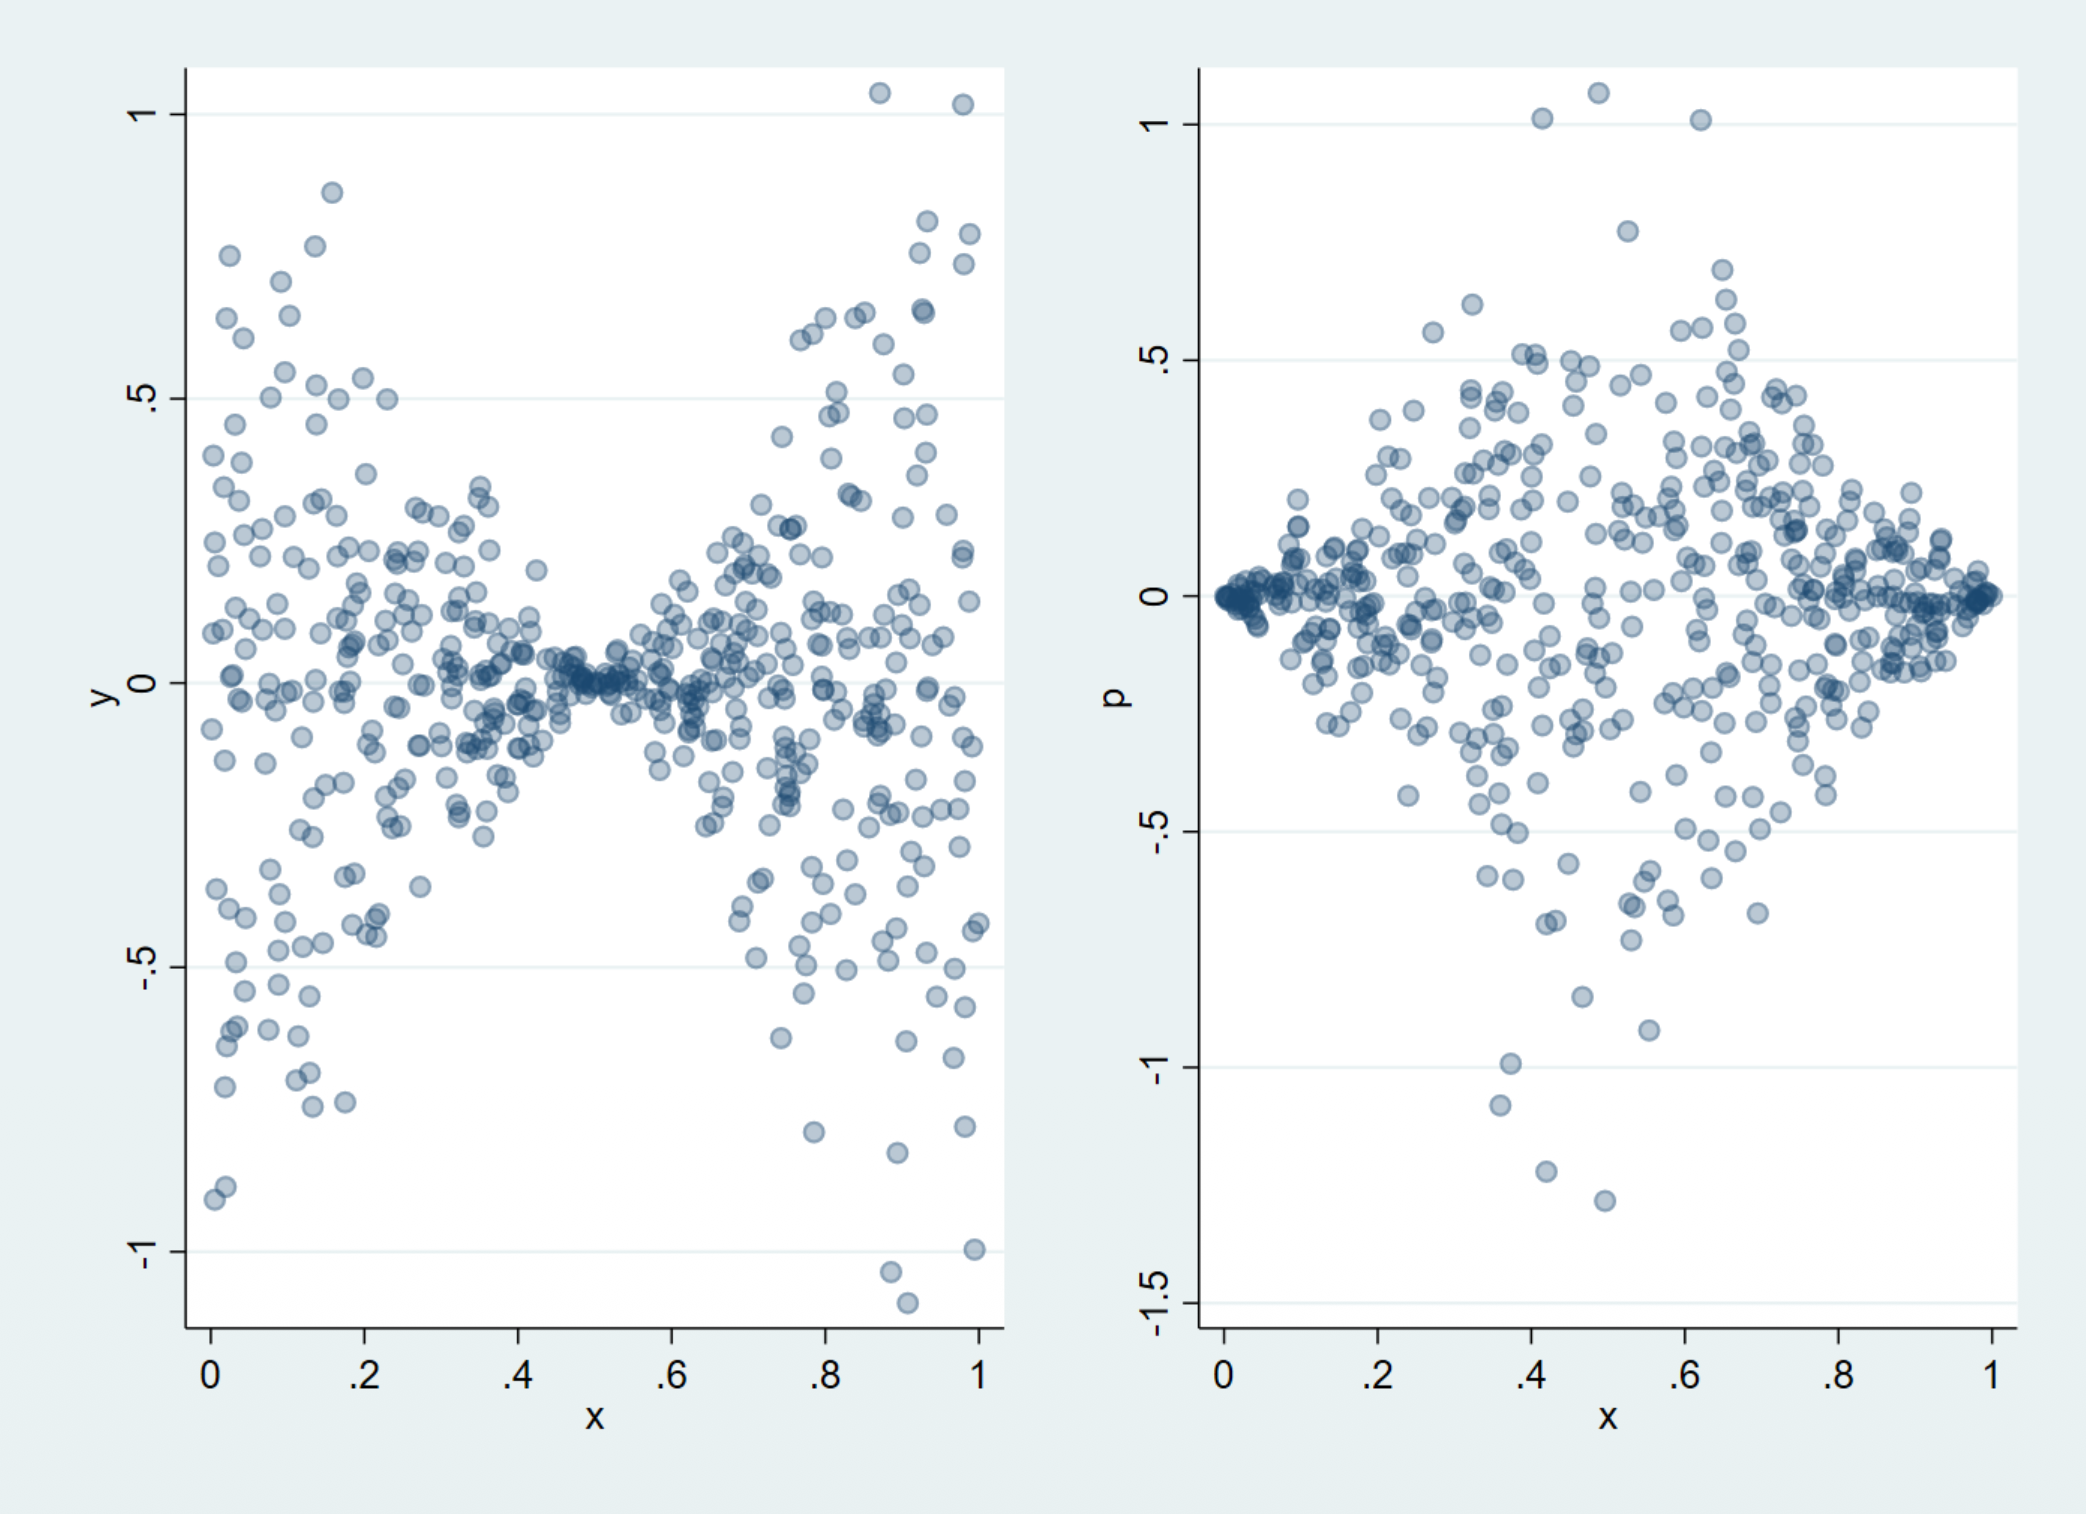
\includegraphics[width=0.78\textwidth]{images/2-12-1}
\end{figure}
Recalling a previous example, it should be much easier to estimate the slope $\beta_1$ from the data on the right, because the concentrations of mass are spread apart.
In fact, the heteroskedastic-robust standard error is smaller than the nonrobust standard error, so it is \emph{not} true that heteroskedastic-robust standard errors are always larger than nonrobust ones.

\begin{remark}	If MLR.5 holds: $\operatorname{Var}(u_i \mid x_i) = \sigma^2$. Since the error variance does not depend on the value of $x_i$, it is called homoskedastic.
	
	If the error variance depends on $x_i$, $u_i$ is heteroskedastic and MLR.5 fails.
	
	If MLR.1-4 are maintained, OLS is still unbiased and consistent under heteroskedasticity, but now the error variance depends on $x_i$: \[
		\operatorname{Var}(u_i \mid x_i) = \sigma_i^2
	,\] which in turn changes $\operatorname{Var}(\hat{\beta}_j \mid X)$.
\end{remark}

	\begin{remark}	If MLR.5 fails, and we use the wrong standard error, we may conclude that our result is significant because we mis-specified the variance of the estimator. This is why generalised least squares is not typically used and instead people do OLS with heteroskedasticity-robust standard errors (using the long form of asymptotic variance).

	Hence, while OLS will be unbiased and consistent, if we end up using the wrong test statistic in our hypothesis test, we may come to a wrong conclusion.

		We also note that using robust standard errors is valid when we have homoskedasticity, but we cannot use non-robust standard errors with heteroskedasticity. (Obviously, but we just need to emphasize this.) For example, consider the two regressions that use nonrobust and robust standard errors and the test statistic $\frac{\hat{\beta}_{\text{lotsize}}}{se\left( \hat{\beta}_{\text{lotsize}} \right)}$.
	\begin{figure}[htpb]
	  \centering
	  \begin{minipage}{0.49\textwidth}
	    \centering
	    \caption{Non-robust standard errors}
	    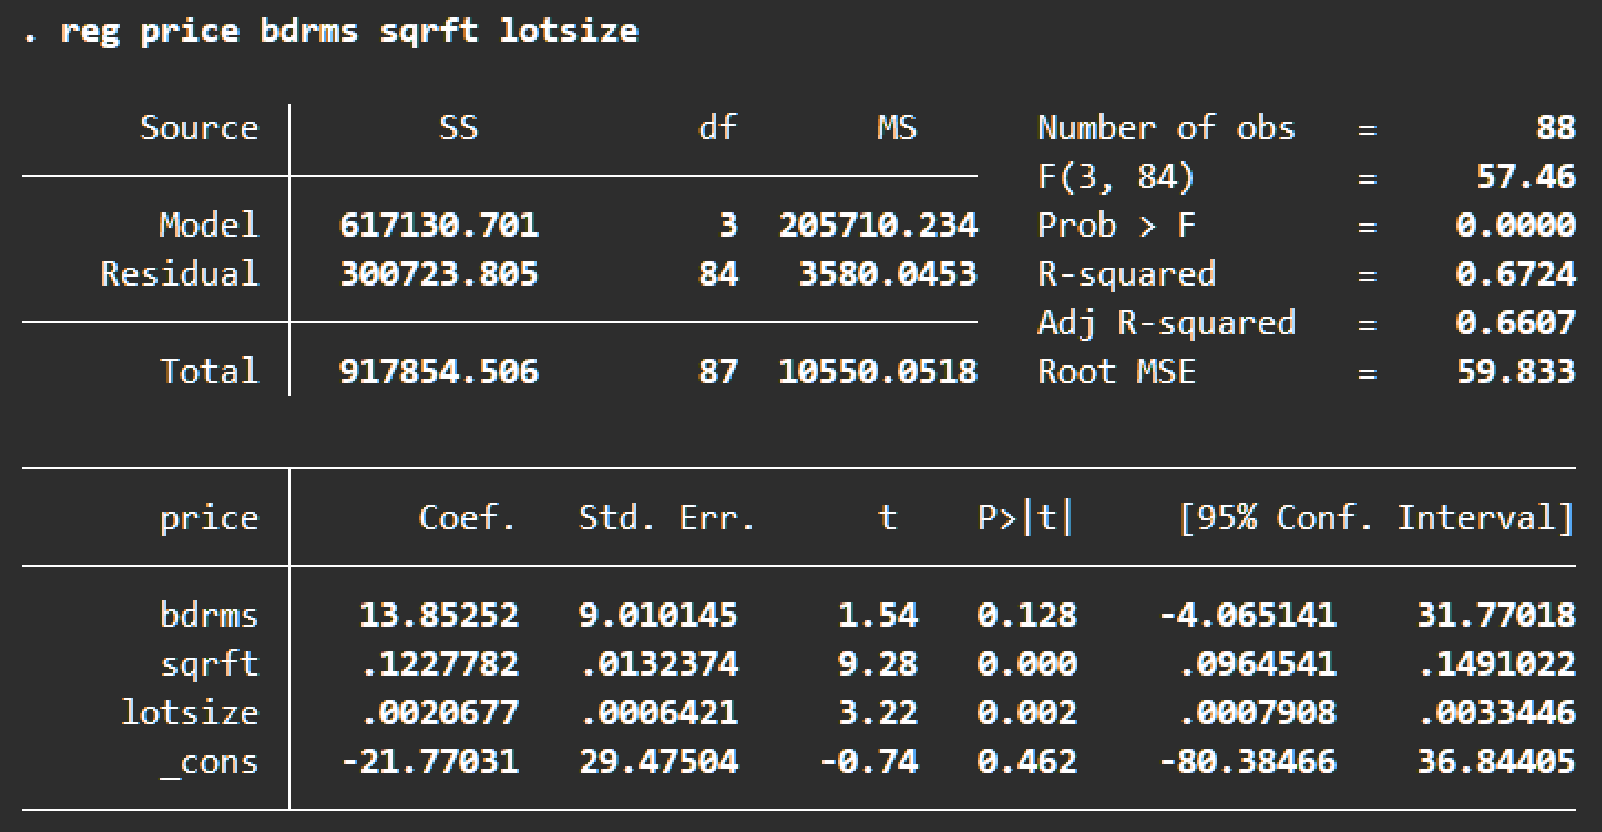
\includegraphics[width=\textwidth]{images/2-12-2}
	  \end{minipage}
	  \hfill
	  \begin{minipage}{0.49\textwidth}
	    \centering
	    \caption{Robust standard errors}
	    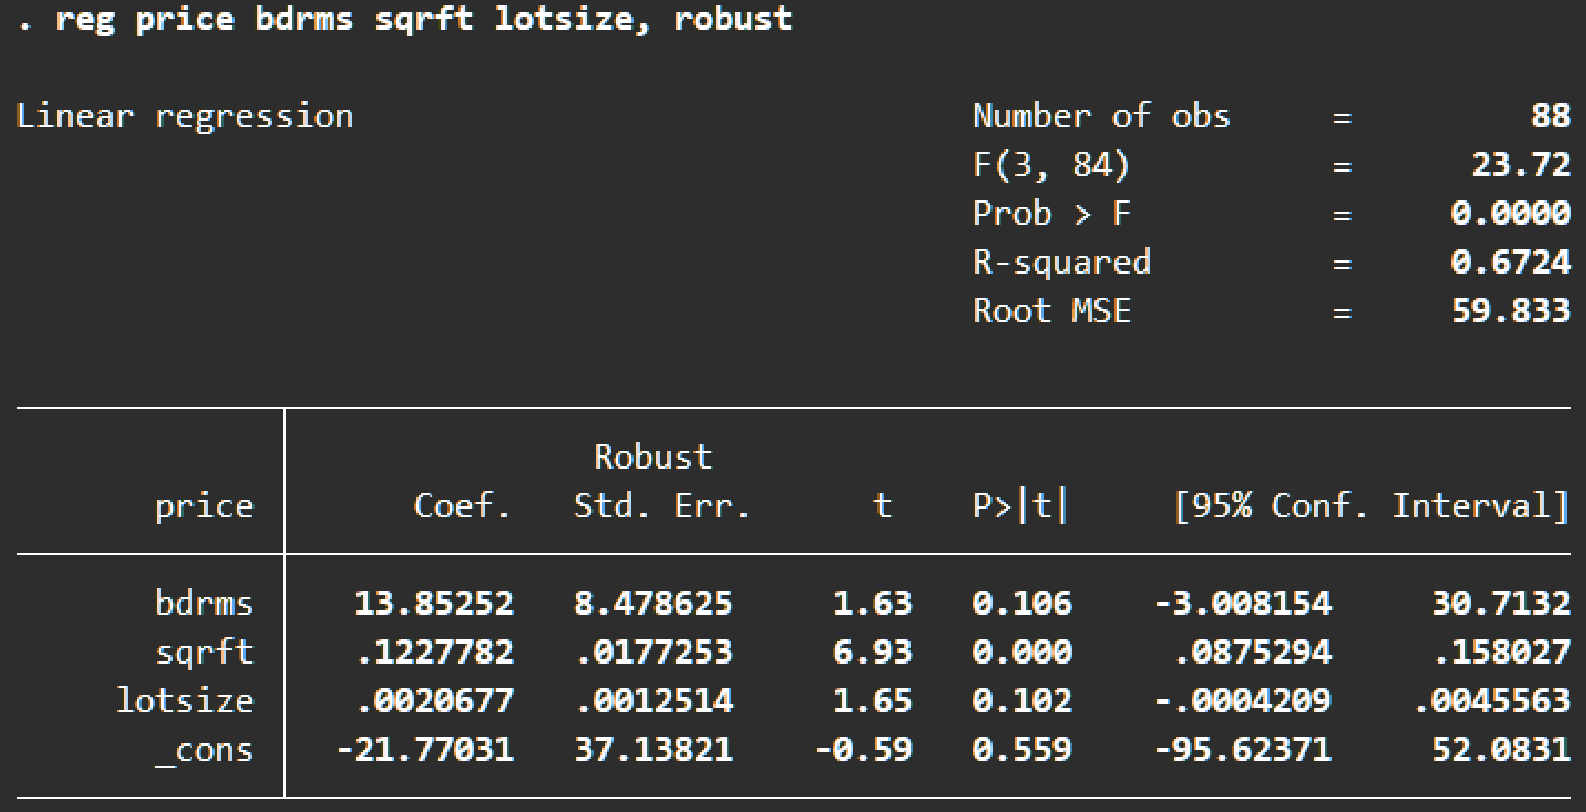
\includegraphics[width=\textwidth]{images/2-12-3}
	  \end{minipage}
	\end{figure}

	When would we ever use non-robust standard errors, then? 
	The advantage of non-robust standard errors is that $t$-stats have exact $t$-distributions under MLR.1-6.
	
	With robust standard errors, we need to use the approximation: \[
		\frac{\hat{\beta}_j - \beta_j}{\operatorname{se}_{\text{rob}}(\hat{\beta}_j)} \approx N(0,1)
	.\] 
	
	In practice, robust standard errors are used because they are valid with any form of heteroskedasticity, while justifying either of MLR.5 (homoskedasticity) or MLR.6 (normality of errors conditional on $X$) is difficult.
\end{remark}

	\begin{proposition}[Variance for individual coefficients]
		When $y_i = \beta_0 + \beta_1 x_{i1} + \cdots + \beta_k x_{ik} + u_i$, we find
		\begin{align*}
			\hat{\beta}_j = \left( X_j' M_{X_{-j}} X_j \right)^{-1} X_j' M_{X_{-j}} Y
		,\end{align*} so \[
			\hat{\beta}_j = \frac{\sum_{i=1}^{n} \hat{r}_{ij} y_i}{\sum_{i=1}^{n} \hat{r}_{ij}^2}
		,\] where $\hat{r}_{ij}$ denotes the $i$-th residual of a regression of $x_j$ on all other regressors.
	
	We find: \[
		\operatorname{Var}(\hat{\beta}_j \mid X) = \frac{\sum_{i=1}^{n} \hat{r}_{ij}^2 \operatorname{Var}(y_i \mid x_i)}{(\sum_{i=1}^{n} \hat{r}_{ij}^2)^2} = \frac{\sum_{i=1}^{n} \hat{r}_{ij}^2 \sigma_i^2}{(\sum_{i=1}^{n} \hat{r}_{ij}^2)^2}
	.\] 
	
	Because $\sigma_i^2$ is unknown, we replace it with $\E\left[u_i^2 \mid X_i\right] = \hat{u}_i^2$ and find: \[
		\widehat{\operatorname{Var}}(\hat{\beta}_j \mid X) = \frac{\sum_{i=1}^{n} \hat{r}_{ij}^2 \hat{u}_i^2}{(\sum_{i=1}^{n} \hat{r}_{ij}^2)^2}
	.\] 
	
	The heteroskedasticity robust standard error is given by\boxednote{Plugging $r_{i 1} = x_i - \overline{x}$ for a regression of $x_1$ onto a constant yields the expression we had in this section's exposition.} \[
		\operatorname{se}(\hat{\beta}_j) = \sqrt{\frac{\sum_{i=1}^{n} \hat{r}_{ij}^2 \hat{u}_i^2}{(\sum_{i=1}^{n} \hat{r}_{ij}^2)^2}}
	.\] 
\end{proposition}

\section{Weighted Least Squares}

\begin{proposition}[Weighted least squares transformation]
	If we knew the error variance $\sigma_i^2$, we could transform the model: \[
		\frac{y_i}{\sigma_i} = \left( \frac{1}{\sigma_i}, \frac{x_{i1}}{\sigma_i}, \ldots, \frac{x_{ik}}{\sigma_i} \right) \beta + \frac{u_i}{\sigma_i}
	.\] 

Notice that this model still satisfies MLR.4 since $\sigma_i$ only depends on $x_i$: \[
	\E\left( \frac{u_i}{\sigma_i} \mid x_i \right) = \frac{1}{\sigma_i} \E(u_i \mid x_i) = 0
.\] 

MLR.1-3 are unaffected, since multiplying each row of $X$ by a non-zero constant does not cause collinearity or change the interpretation of the model.

However, MLR.5 now holds, because \[
	\E\left[ \left( \frac{u_i}{\sigma_i} \right)^2 \mid \frac{x_i}{\sigma_i} \right] = \E\left[ \E\left[ \left( \frac{u_i}{\sigma_i} \right)^2 \mid x_i \right] \mid \frac{x_i}{\sigma_i} \right]
,\] and \[
	\E\left[ \left( \frac{u_i}{\sigma_i} \right)^2 \mid x_i \right] = \frac{1}{\sigma_i^2} \E(u_i^2 \mid x_i) = \frac{\sigma_i^2}{\sigma_i^2} = 1
.\] 

	OLS on the transformed model gives the best linear unbiased estimator of $\beta$ by the Gauss--Markov Theorem.\boxednote{There is some nuance here: Gauss--Markov gives us efficiency conditional on $\left(\frac{x_i}{\sigma_i}\right)$, but we will show in another problem set that it can be efficient conditional on $x$ as well.}
\end{proposition}

We really will just consider weighted least squares with homoskedasticity at the individual level. Geralized least squares weights based on the error variance, but this is beyond the scope of this course.

\begin{example}[WLS: Grouped Data]
	Suppose the model for observation $i$ is \[
		y_i = \beta_0 + \beta_1 x_i + u_i
	,\] where MLR.1-5 hold. Let $\operatorname{Var}(u \mid x) = \sigma^2$.
	
	Our observations are group averages e.g. mean age/income by zip code.
	
	There are $K$ groups $k = 1, \ldots, K$, and we observe \[
		\bar{y}_k = \frac{1}{n_k} \sum_{i \in \text{Group } k} y_i; \quad \bar{x}_k = \frac{1}{n_k} \sum_{i \in \text{Group } k} x_i
	\] for each $k = 1, \ldots, K$.
	
	We would actually run the regression on zip-code level data, so we make clear that the model written for averages is: \[
		\bar{y}_k = \beta_0 + \beta_1 \bar{x}_k + \bar{u}_k
	.\] 
	The error variance is \[
		\operatorname{Var}(\bar{u}_k \mid X) = \frac{\sigma^2}{n_k}
	.\] 
	This would actually give a different estimator of $\beta$ (since the weighting is uniform across zip codes, and not individuals as in the granular regression), and has heteroskedasticity.

	Hence, we should multiply by $\sqrt{n_k}$ to restore MLR.5\footnote{Note: we only recover homoskedasticity with this simple weighting because the original individual data was homoskedastic.} and estimate the following by OLS: \[
		\sqrt{n_k} \cdot \bar{y}_k = \beta_0 \cdot \sqrt{n_k} + \beta_1 \sqrt{n_k} \cdot \bar{x}_k + \sqrt{n_k} \cdot \bar{u}_k
	.\] 
	Here, $\operatorname{Var}(\sqrt{n_k} \cdot \bar{u}_k \mid X) = n_k \operatorname{Var}(\bar{u}_k \mid X) = \sigma^2$.
\end{example}

\section{Regression Specification}

\begin{remark}	Multiple linear regression can be used to model non-linear patterns in the data.
	
	We discuss:
	\begin{itemize}
		\item Using logarithms and polynomials to model non-linear patterns
		\item Turning continuous variables into qualitative variables
		\item Using qualitative variables to allow categories in the data to have their own coefficients
		\item Using interactions to allow the effect of changing one explanatory variable on the conditional mean to vary with the value of another.
	\end{itemize}
\end{remark}

\begin{remark}[Logarithms]
	Logarithms are often used to approximate proportional changes. For $x'$ close to $x$: \[
		\log(x') - \log(x) \approx \frac{x' - x}{x}
	\] by a first-order Taylor expansion, which is the proportional change from $x$ to $x'$.
	
	Several specifications used for conditional mean: \begin{align*}
		\E(y \mid x = t) &\approx \alpha + \beta \log(t) \quad \text{``level-log''} \\
		\E(\log(y) \mid x = t) &\approx \alpha + \beta t \quad \text{``log-level''} \\
		\E(\log(y) \mid x = t) &\approx \alpha + \beta \log(t) \quad \text{``log-log''}
	.\end{align*}
\end{remark}

Differentiating a conditional expectation is difficult, since we don't want to move the derivative operator in the expectation. Thus, the easiest log model to interpret is the log-level specification.

\begin{remark}[level-log specification]
	Consider $\E\left[y \mid x = t\right] = \alpha + \beta \ln{\left(t\right)}$.

	We have \begin{align*}
		\E(y \mid x = t + \Delta t) - \E(y \mid x = t) &\approx \beta[\log(t + \Delta t) - \log(t)] \\
		&\approx \beta \cdot \frac{\Delta t}{t} \\
		&= \frac{\beta}{100} \cdot \frac{100\Delta t}{t}
	,\end{align*} so $\beta/100$ is approximately the change in the conditional mean of $y$ when $t$ increases by $1\%$.\boxednote{This percentage interpretation is only valid for a causal interpretation, in that we examine a level of $t$ and error, then see the change in $y$ when increasing $t$. But we cannot differentiate a random variable with respect to another carelessly.}
\end{remark}

\begin{remark}[log-level specification]
	We have \[
		\E(\log(y) \mid x = t + 1) - \E(\log(y) \mid x = t) \approx \beta
	.\] 
	
		Expectations don't pass through non-linear functions (e.g. Jensen), but the following approximation leads to the common interpretation that a unit increase in $x$ is associated with a $\beta\%$ change in the mean of $y$:\boxednote{Jensen's inequality means $\E[\log y \mid x]$ need not equal $\log \E[y \mid x]$. The approximation is exact when $y \mid x$ is log-normal.} \begin{align*}
			\beta &\approx \E(\log(y) \mid x = t + 1) - \E(\log(y) \mid x = t) \\
			&\approx \log(\E(y \mid x = t + 1)) - \log(\E(y \mid x = t)) \\
			&\approx \frac{\E(y \mid x = t + 1) - \E(y \mid x = t)}{\E(y \mid x = t)}
	,\end{align*} so $100\beta$ is approximately the percentage change in the mean of $y$ resulting from a unit increase in $x$.
	
	Alternatively, exponentiating the first approximation and subtracting $1$ gives: \begin{align*}
		\exp(\beta) - 1 &\approx \exp(\E(\log(y) \mid x = t + 1) - \E(\log(y) \mid x = t)) - 1 \\
		&= \frac{\exp(\E(\log(y) \mid x = t + 1)) - \exp(\E(\log(y) \mid x = t))}{\exp(\E(\log(y) \mid x = t))}
	.\end{align*}
	Given that $\exp(x) \approx 1 + x$ when $x \approx 0$, the left hand side is approximately equal to $\beta$ if $\beta \approx 0$.
	
	We can therefore interpret $\beta$ as the proportional change in the conditional geometric mean of $y$ given a unit increase in $x$, holding the error term fixed.
\end{remark}

\begin{remark}[log-log specification]
	Now we have \[
		\E(\log(y) \mid x = t + \Delta t) - \E(\log(y) \mid x = t) \approx \beta[\log(t + \Delta t) - \log(t)]
	.\] 
	
	Combining the approximations for log-level and level-log gives: \[
		\frac{\E(y \mid x = t + \Delta t) - \E(y \mid x = t)}{\E(y \mid x = t)} \approx \beta \cdot \frac{\Delta t}{t}
	,\] so a $1\%$ increase in $t$ is associated with a $\beta\%$ change in the conditional mean of $y$ (also known as an elasticity).
\end{remark}

\begin{example}[Returns to experience]
	Consider the approximation: \[
		\E(\text{wage} \mid \text{exper}) \approx \beta_0 + \beta_1 \text{exper} + \beta_2 \text{exper}^2
	.\] 
	
	Experience estimated to have a diminishing marginal effect on wage.
	
	Turning point estimated where \[
		\frac{\partial \E(\text{wage} \mid \text{exper} = e^*)}{\partial e} = \hat{\beta}_1 + 2\hat{\beta}_2 e^* = 0 \implies e^* = -\frac{\hat{\beta}_1}{2\hat{\beta}_2} \approx 24
	.\] 
\end{example}

\begin{remark}[Returns to Experience]
	Issues with a causal interpretation:
	\begin{itemize}
		\item Omitted Variables Bias: Education impacts wage and may be correlated with/interact with exper or exper$^2$.
		\item Functional form misspecification: $w$ or $\ln(w)$? Quadratic in experience?
	\end{itemize}
	
	Average partial effect: What is the marginal effect of experience? \[
		\frac{\partial \E(\text{wage} \mid \text{exper} = e)}{\partial e} = \beta_1 + 2\beta_2 e
	.\] 
	The effect of experience diminishes if $\beta_2 < 0$. We can estimate the average partial effect: \[
		\widehat{\text{APE}} = \frac{1}{n} \sum_{i=1}^{n} (\hat{\beta}_1 + 2\hat{\beta}_2 \text{exper}_i) = \hat{\beta}_1 + 2\hat{\beta}_2 \overline{\text{exper}}_n
	.\] 
\end{remark}

\begin{remark}[Dummy Variables]
	Suppose we want to measure the difference in average wages between the tech industry and all other industries.
	
	Use a ``Dummy Variable'' to denote categories within data.
\end{remark}

\begin{remark}[Continuous variables to categorical variables]
	Suppose we are interested in estimating store sales by age category:
	\begin{itemize}
		\item Observe sales figures and age of customers.
		\item Create $k$ categories as follows: \[
			d_{i1} = \begin{cases}
				1 & \text{if } i \text{ is between 0-18 years of age} \\
				0 & \text{otherwise}
			\end{cases}
		\] \[
			d_{i2} = \begin{cases}
				1 & \text{if } i \text{ is between 18-25 years of age} \\
				0 & \text{otherwise}
			\end{cases}
		\] \[
			\vdots
		\] \[
			d_{ik} = \begin{cases}
				1 & \text{if } i \text{ is 75+ years of age} \\
				0 & \text{otherwise}
			\end{cases}
		\] 
	\end{itemize}
	
	Note: Groups are mutually exclusive ($d_{ij} d_{ik} = 0$ when $i \ne j$) and exhaustive ($d_{i1} + \cdots + d_{ik} = 1$).
	
	Means WLOG we can describe average sales by age category using \[
		\E(y_i \mid d_{i1}, \ldots, d_{ik}) = \beta_1 d_{i1} + \beta_2 d_{i2} + \cdots + \beta_k d_{ik}
	,\] where intercept is excluded to avoid perfect collinearity.
	
	Can also specify \[
		\E(y_i \mid d_{i1}, \ldots, d_{ik}) = \alpha_0 + \alpha_1 d_{i1} + \alpha_2 d_{i2} + \cdots + \alpha_{k-1} d_{ik-1}
	.\] 
	
	Note: \[
		\alpha_1 = \E(y \mid d_{i1} = 1, \ldots, d_{ik} = 0) - \E(y \mid d_{i1} = 0, \ldots, d_{ik} = 1)
	\] is interpreted as the difference in average spend between the youngest and oldest age categories.
	
	Excluding the dummy variable for the oldest category specifies that category as the base group.
	
	Intercept $\alpha_0$ is the mean for the base group.
	
	$\alpha_j$ represents difference in means between group $j$ and base group.
\end{remark}

\begin{remark}[Kinks and Jumps]
	Describe credit limits offered to new customers as a function of credit score.
	
	Sometimes outcome will change sharply at a cutoff. Suppose $y$ is credit limit and $x$ is credit score.
	
	Suppose only two categories of credit: 'Good' and 'Excellent'.
	
	Features:
	\begin{itemize}
		\item Sharp discontinuity in credit limit as soon as individual crosses 'Excellent' boundary
		\item Each additional unit of credit score improves credit limit more for individuals with excellent credit (Kink)
	\end{itemize}
	
	Let \[
		d_i = \begin{cases}
			1 & \text{if individual } x_i \ge 0.5 \\
			0 & \text{if individual } x_i < 0.5
		\end{cases}
	\] 
	
	Model: \begin{align*}
		y_i &= \beta_0 + \beta_1 x_i + d_i(\gamma + \delta x_i) + \epsilon_i \\
		&= \beta_0 + \beta_1 x_i + \gamma d_i + \delta d_i x_i + \epsilon_i
	.\end{align*}
	
	When $x_i < a$: $\E(y_i \mid x = x_i) = \beta_0 + \beta_1 x_i$.
	
	When $x_i \ge a$: $\E(y_i \mid x = x_i) = (\beta_0 + \gamma) + (\beta_1 + \delta) x_i$.
	
	Note: not all parameters have a useful interpretation: $\beta_0 + \gamma$ is the credit limit an individual with 'Excellent' credit would receive if their credit score were $0$ (We could never observe such individuals in the data).
	
	$\delta$ represents the additional return to credit score for individuals with excellent credit.
	
	Jump: $\gamma + \delta \cdot 0.5$.
\end{remark}

\begin{remark}[Saturated Regression]
	Describe wages in tech vs. not in tech, both inside and outside california: \[
		\E(W \mid T, C) = \beta_0 + \beta_1 T + \beta_2 C + \beta_3 T \cdot C
	.\] 
	We call this a saturated regression since it has one parameter for each possible value of the regressors: \[
		(T, C) \in \{(0,0), (1,0), (0,1), (1,1)\}
	.\] 
	
	The equality holds by construction, not because of an additional assumption about linearity of the conditional mean.
	
	Could also specify \[
		\E(W \mid T, C) = \alpha_0 (1-T) \cdot (1-C) + \alpha_1 T \cdot (1-C) + \alpha_2 (1-T) \cdot C + \alpha_3 T \cdot C
	.\] 
	
	Only difference is in interpretation of parameters: \begin{align*}
		\E(W \mid T = 0, C = 0) &= \beta_0 = \alpha_0 \\
		\E(W \mid T = 1, C = 0) &= \beta_0 + \beta_1 = \alpha_1 \\
		\E(W \mid T = 0, C = 1) &= \beta_0 + \beta_2 = \alpha_2 \\
		\E(W \mid T = 1, C = 1) &= \beta_0 + \beta_1 + \beta_2 + \beta_3 = \alpha_3
	.\end{align*}
	
	$\beta_1$ represents difference in average wages in tech vs. not for employees outside california.
	
	$\beta_2$ represents difference in average wages in california vs. not for employees not in tech.
	
	$\beta_3$ represents a ``difference in differences''. For example: \begin{align*}
		\beta_3 &= [(\beta_0 + \beta_1 + \beta_2 + \beta_3) - (\beta_0 + \beta_2)] - [(\beta_0 + \beta_1) - \beta_0] \\
		&= [\E(W \mid T = 1, C = 1) - \E(W \mid T = 0, C = 1)] \\
		&\quad - [\E(W \mid T = 1, C = 0) - \E(W \mid T = 0, C = 0)]
	.\end{align*}
	
	This is the difference (between california and not) in differences in wages inside and outside tech.
\end{remark}

	\begin{remark}[Interactions]
		An interaction is a product of two regressors. e.g. \[
			\text{wage} = \beta_0 + \beta_1 \text{educ} + \beta_2 \text{exper} + \beta_3 \text{educ} \cdot \text{exper} + \epsilon
	.\] 
	
		If $\E(\epsilon \mid \text{educ}, \text{exper}) = 0$, we have: \[
			\frac{\partial}{\partial \text{exper}} \E(\text{wage} \mid \text{educ}, \text{exper}) = \beta_2 + \beta_3 \text{educ}
		,\] so if $\beta_3 > 0$, average wage for those with more education differs more across experience levels.
	\end{remark}

\section{Summary}

\begin{remark}[Model and estimator]
	\leavevmode\hfill\break
	\textbf{Model}: $y = x'\beta + u$ with $\E\left[xu\right] = 0$. \\
	\textbf{Estimator}: $\hat{\beta}^{OLS} = (X'X)^{-1}X'Y$. \\
	\textbf{Interpretation}: each coefficient is the slope of the conditional mean with the remaining regressors held fixed.
\end{remark}

\begin{remark}[Finite-sample inference under normality]
	Suppose $Y \mid X \sim N(X\beta,\sigma^2 I_n)$. Exact conditional distributions:
	\[
		\begin{aligned}
			\hat{\beta} \mid X &\sim N\left(\beta,\sigma^2 (X'X)^{-1}\right), \\
			\hat{\sigma}^2 = \frac{SSR}{n-k} &\sim \frac{\sigma^2}{n-k}\chi^2_{n-k}
		\end{aligned}
	.\]
	The key finite-sample fact is that $\hat{\beta}-\beta$ and $\hat{\sigma}^2$ are conditionally independent, which yields exact $t_{n-k}$ tests and confidence intervals.
\end{remark}

\begin{remark}[Large-sample inference]
	Without normality, asymptotic normality replaces exact finite-sample formulas:
	\[
		\sqrt{n}(\hat{\beta}_n-\beta) \xrightarrow{d} N(0,V)
	.\]
	Single restrictions use asymptotic $z$-tests and confidence intervals, while multiple restrictions use $\chi^2_p$ statistics and ellipsoidal confidence sets for $R\beta$.
\end{remark}

\begin{remark}[Homoskedastic vs.\ heteroskedastic inference]
		\begin{center}
		\small
		\renewcommand{\arraystretch}{1.1}
		\begin{tabular}{p{0.20\linewidth}p{0.27\linewidth}p{0.33\linewidth}}
			\toprule
			Case & Standard error formula & Inference to use \\
			\midrule
			Homoskedastic, normal & $\hat{\sigma}^2(X'X)^{-1}$ & Exact $t$ / exact finite-sample \\
			Homoskedastic, large sample & $\hat{\sigma}^2(X'X)^{-1}$ & Asymptotic normal / $\chi^2$ \\
			Heteroskedastic & $(X'X)^{-1}X'\hat{\Omega}X(X'X)^{-1}$ & Robust asymptotic normal / $\chi^2$ \\
			\bottomrule
		\end{tabular}
		\end{center}
		Robust standard errors are valid in both homoskedastic and heteroskedastic settings, but exact $t$ inference requires the stronger homoskedastic-normal setup.
\end{remark}

\begin{remark}[Weighted least squares]
	If $\operatorname{Var}(u_i \mid x_i) = \sigma_i^2$ is known, divide the $i$-th observation by $\sigma_i$ to restore homoskedasticity. OLS on the transformed model is WLS and is efficient within the class of linear unbiased estimators under the transformed homoskedastic model.
\end{remark}

\begin{remark}[Regression specifications]
	Common specifications and their interpretation:
	\begin{itemize}
		\item \textbf{Level-log}: $\beta/100$ is the change in $\E(y \mid x)$ for a $1\%$ increase in $x$.
		\item \textbf{Log-level}: $100\beta$ approximates the percent change in $\E(y \mid x)$ for a one-unit increase in $x$.
		\item \textbf{Log-log}: $\beta$ is an elasticity.
		\item \textbf{Dummies/interactions}: allow group-specific intercepts, slopes, and difference-in-differences style comparisons.
	\end{itemize}
\end{remark}

\styledchapter{Selection on Observables}

\begin{remark}	So far we have considered counterfactuals using linear regression:
	\begin{itemize}
		\item How much does earnings potential increase with another year of experience, holding all else fixed?
		\item How much does an additional bedroom increase house price, holding floor area/lot size/air pollution (and all else) fixed?
	\end{itemize}
	OLS estimates proportional to ``partial correlations'' between outcome and regressors. ``Holding fixed'' other observable factors in this way answers counterfactual question if $y = x'\beta + u$ and $\E\left[xu\right] = 0$. In particular, $\E\left[xu\right] = 0$ implies
	\[
		\beta = \E\left[xx'\right]^{-1}\E\left[xy\right]
	,\]
	so (scaled) partial correlations are partial (causal) effects, and scaled partial correlations can be estimated.
\end{remark}

\begin{definition}[Rubin Causal Model]
	We can think about counterfactuals as `potential outcomes' under different `treatments':
	\begin{itemize}
		\item Earnings with college degree, $y(1)$, and without $y(0)$.
		\item Health outcome with drug A, $y(1)$, vs. drug B, $y(0)$.
		\item Productivity with job training, $y(1)$ vs. without, $y(0)$.
	\end{itemize}
	Define individual treatment effect for individual $i$ as $y_i(1) - y_i(0)$. Denote treatment status of individual $i$ by $D_i \in \left\{0, 1\right\}$.
\end{definition}

\section{Motivation: Store Upgrades}

Consider $100$ stores where we are trying to measure the effect of receiving an interior upgrade on sales.

\begin{example}[Store Upgrades]
	$y_i(1)$ denotes sales store $i$ would observe with an upgrade. $y_i(0)$ denotes sales store $i$ would observe without an upgrade. The outcome observed is
	\[
		Y_i =
		\begin{cases}
			y_i(1) & \text{if store $i$ is upgraded,} \\
			y_i(0) & \text{if not.}
		\end{cases}
	\]
	In other words,
	\[
		Y_i = y_i(1)D_i + y_i(0)\left(1-D_i\right)
	,\]
	where $D_i$ is an indicator for if store $i$ received an upgrade.

	We never observe the individual causal effect $y_i(1)-y_i(0)$ for any store because only one of the two potential outcomes is ever observed. However, we can try to measure average effects across treated and untreated stores by comparing averages:
	\begin{itemize}
		\item e.g. Average Treatment Effect in store population (ATE): $\E\left[y(1)-y(0)\right]$.
		\item e.g. Average Treatment Effect on the treated (ATT): $\E\left[y(1)-y(0) \mid D=1\right]$.
		\item e.g. Average Treatment Effect on untreated (ATU): $\E\left[y(1)-y(0) \mid D=0\right]$.
	\end{itemize}

	What is identified from $\E\left[Y \mid D\right]$?

	First write out the conditional mean of $Y \mid D$:
	\begin{align*}
		\E\left[Y \mid D=1\right] &= \E\left[y(1)D + y(0)(1-D) \mid D=1\right] \\
		&= \E\left[y(1) \mid D=1\right] \\
		\E\left[Y \mid D=0\right] &= \E\left[y(1)D + y(0)(1-D) \mid D=0\right] \\
		&= \E\left[y(0) \mid D=0\right]
	.\end{align*}
	We can observe $\E\left[y(1) \mid D=1\right]$ and $\E\left[y(0) \mid D=0\right]$. The data reveal an estimate of the `naive comparison':
	\[
		\E\left[y(1) \mid D=1\right] - \E\left[y(0) \mid D=0\right]
	,\]
	which is ATT plus selection effects.
\end{example}

\begin{remark}    Examining stores that are upgraded, not upgraded, and the whole population, we might see that
	\begin{center}
		\scriptsize
		\renewcommand{\arraystretch}{1.15}
		\begin{tabular}{p{0.24\linewidth}p{0.18\linewidth}p{0.18\linewidth}p{0.18\linewidth}}
			& $D_i = 0$ & $D_i = 1$ & All \\
			\hline
			average sales if upgraded
				& $\E[y(1)\mid D=0]=?$ 
				& $\E[y(1)\mid D=1]=100$
				& $\E[y(1)]=?$ \\
			average sales if not upgraded
				& $\E[y(0)\mid D=0]=50$
				& $\E[y(0)\mid D=1]=?$
				& $\E[y(0)]=?$ \\
			difference
				& $\E[y(1)-y(0)\mid D=0]=ATU$
				& $\E[y(1)-y(0)\mid D=1]=ATT$
				& $\E[y(1)-y(0)]=ATE$
		\end{tabular}
	\end{center}
\end{remark}

\begin{proposition}[Relationship between ATE, ATT, ATU]
	We can decompose the ATE as follows:
		\begin{align*}
			\E\left[y(1)-y(0)\right]
			&= \E\left[y(1)-y(0) \mid D=1\right]\P\left(D=1\right) \\
			&\quad + \E\left[y(1)-y(0) \mid D=0\right]\P\left(D=0\right) \\
			&= ATT \cdot \P\left(D=1\right) + ATU \cdot \P\left(D=0\right)
		.\end{align*}
\end{proposition}
\begin{proof}
	By the law of iterated expectation.
\end{proof}

\begin{proposition}[Regression and selection bias]
	Write out the conditional mean of $Y \mid D$:
	\[
		\E\left[Y \mid D=1\right] = \E\left[y(1) \mid D=1\right], \qquad
		\E\left[Y \mid D=0\right] = \E\left[y(0) \mid D=0\right]
	.\]
	It follows that
	\[
		\E\left[Y \mid D\right] = \beta_0 + \beta_1 D
	,\]
	where
	\[
		\beta_0 = \E\left[y(0) \mid D=0\right], \qquad
		\beta_1 = \E\left[y(1) \mid D=1\right] - \E\left[y(0) \mid D=0\right]
	.\]
\end{proposition}
\begin{proof}
	Thus $\beta_1$ equals the naive comparison. Moreover,
	\begin{align*}
		\beta_1
		&= \E\left[y(1) \mid D=1\right] - \E\left[y(0) \mid D=0\right] \\
		&= \underbrace{\E\left[y(1) \mid D=1\right] - \E\left[y(0) \mid D=1\right]}_{\text{ATT}}
		+ \underbrace{\E\left[y(0) \mid D=1\right] - \E\left[y(0) \mid D=0\right]}_{\text{Selection Bias}}
	.\end{align*}
		$\beta_1$ measures the average effect on stores that were upgraded (ATT) but is offset by ``selection bias'' in $y(0)$, which measures differences in average sales in the absence of upgrades.\boxednote{Equivalent decompositions are $\beta_1=ATT+SB_{y(0)}$ and $\beta_1=ATU+SB_{y(1)}$.}
\end{proof}

\begin{remark}	There is a big difference between selection bias in $y(0)$ vs selection bias in $y(1)$.
	
	For selection bias in $y(0)$ but not in $y(1)$, consider factories that do not get training who have scrap rates of $0.01$, factories that do get training who initially have scrap rates of $0.05$, but then $0.01$ after training.

	For selection bias in $y(1)$ but not $y(0)$, consider factories all with the same scrap rate, then factory managers who only opt into training if their employees are trainable, whose scrap rates go down after treatment. If the factories who opted out of training would have had the same scrap rate as before even if they received training, we would have selection bias in $y(1)$ only.

	Furthermore, the naive comparison can equal the ATE if the probability of selection and the magnitude of ATT/ATU cancel each other out, but this is generally not the case.
\end{remark}

\section{Random assignment}

\begin{definition}[Random assignment]
	How treatment is assigned determines whether selection bias is present. Random assignment:
	\[
		D_i \ind \left(y_i(0), y_i(1)\right)
	.\]
	This says treatment choice/assignment is independent of outcomes under treatment and no treatment.
\end{definition}

\begin{proposition}[Random assignment implies $\beta_1 = ATE$]
	Under random assignment,
	\[
		\E\left[y(0) \mid D\right] = \E\left[y(0)\right], \qquad
		\E\left[y(1) \mid D\right] = \E\left[y(1)\right]
	,\]
	i.e.\ the treatment and control groups are representative of the entire population. Hence,
	\[
		\beta_1 = \E\left[y(1)\right] - \E\left[y(0)\right] = ATE
	.\]
\end{proposition}
\begin{proof}
	\begin{align*}
		\beta_1
		&= \E\left[y(1) \mid D=1\right] - \E\left[y(0) \mid D=0\right] \text{ (naive comparison)}\\
		&= \E\left[y(1)\right] - \E\left[y(0)\right] \\
		&= ATE
	.\end{align*}
	Hence, under randomized treatment assignment, estimating a linear regression (which gives a coefficient that is the naive estimator) produces an unbiased estimate of the ATE.
\end{proof}

\begin{remark}[Multiple possible treatments]
	Suppose in a randomized clinical trial there is a control group and $k$ possible treatments for a particular health condition. Suppose participants are randomly assigned to either control or one of the treatments. Let
	\[
		x_{i1} =
		\begin{cases}
			1 & \text{if $i$ receives treatment 1,} \\
			0 & \text{otherwise,}
		\end{cases}
		\qquad
		x_{i2} =
		\begin{cases}
			1 & \text{if $i$ receives treatment 2,} \\
			0 & \text{otherwise,}
		\end{cases}
	\]
	and similarly for $x_{ik}$. There are now $k+1$ potential outcomes $y_i(0), y_i(1), \ldots, y_i(k)$ and
	\[
		Y_i = y_i(0) + x_{i1}\left(y_i(1)-y_i(0)\right) + \cdots + x_{ik}\left(y_i(k)-y_i(0)\right)
	.\]
	Now let $x_i = \left(1, x_{i1}, \ldots, x_{ik}\right)'$. We have
	\[
		\E\left[Y_i \mid x_i\right] = \beta_0 + \beta_1 x_{i1} + \cdots + \beta_k x_{ik}
	,\]
	where $\beta_0 = \E\left[y(0)\right]$ and, for each $j = 1, \ldots, k$, $\beta_j = \E\left[y(j)-y(0)\right]$.

	If we have random assignment, 
	\begin{align*}
		\E\left[Y_i \mid x_{i,1} = 0,\ldots,x_{i,k} = 0\right] &= \E\left[y_i(0) \mid x_{i,1} = 0 ,\ldots, x_{i,k} = 0\right] = \E\left[y_i(0)\right] \\
		\E\left[Y_i \mid x_{i,1} = 0 ,\ldots,x_{i,k} = 1\right] &= \E\left[y_i(k) \mid x_{i,1}= 0,\ldots,x_{i,k} = 1\right] = \E\left[y_i(k)\right] 
	.\end{align*}

	We can test whether these effects are statistically different from zero (or from each other) by forming appropriate hypotheses, e.g. $H_0:\beta_k=0$ or $H_0:\beta_1=\beta_2$.
\end{remark}

\section{Nonrandom assignment}

Now we examine when we don't have random assignment and in fact have selection bias.

\begin{example}[Job Training]
	JTRAIN98 contains data on labor market outcomes for men, some of whom enrolled in a job training program in 1997. Only men who had low earnings were allowed to enroll in the program:

	Considering the potential outcomes of earnings in 1998 without and with training, we see that the potential outcomes are correlated with treatment, because those who were eligible to be treated were lower income to begin with. (We expected both potential outcomes to be negatively correlated with $D$.) But conditioning on earnings in 1996 may remove this.

	\begin{itemize}
		\item Whether or not individual took training in 1997: $train = 1$ if training taken
		\item Earnings in 1998 (in \$1000s): $earn98$
		\item Earnings in 1996 (in \$1000s): $earn96$
		\item Whether or not individual is married: $married = 1$ if married
		\item Education in years of schooling: $educ$
		\item Age in years: $age$
	\end{itemize}
	First, compute naive comparison by running regression:
	\[
		earn98 = \beta_0 + \beta_1 train + \epsilon
	.\]Then $\hat{\beta}_1 = \overline{y}_{train} - \overline{y}_{not train} \xrightarrow{p} \E\left[Y \mid D = 1\right] - \E\left[Y \mid D = 0\right] $.
	$\hat{\beta}_1$ is a comparison of means between individuals who did/did not take training, and indicates that individuals who took training earned \$2050 less on average in 1998. This is because the selection bias is outweighing the treatment effect.

	Or, controlling for observable characteristics:
	\[
		earn98 = \beta_0 + \beta_1 train + \beta_2 educ + \beta_3 age + \beta_4 married + \beta_5 earn96 + \epsilon
	.\]

	The regression results show a negative coefficient on training when not controlling for observable characteristics, but a statistically significant positive coefficient on training when controlling for observable characteristics.
\end{example}
\begin{definition}[Covariate balance test]
	One way random assignment is justified statistically is by a ``balance test.'' We want to see if individuals with particular covariates are more likely to select into treatment. Practically: Regress treatment dummy $D_i$ on observable characteristics $x_i$:
	\[
		D_i = \gamma_0 + x_i'\gamma_1 + \epsilon_i
	.\]
	Conduct $F$-test of $H_0:\gamma_1=0$ vs. $H_1:\gamma_1 \ne 0$.\boxednote{The $F$-test is the finite sample analog of the test of multiple linear restrictions ($t$-test vs. $z$-test).}
\end{definition}

\begin{remark}[Issues with balance tests]
	The goal of a balance test is to show that $D$ is independent of potential outcomes. But this is not something that is measurable.
	A balance test can show that $x$ is uncorrelated with potential outcomes, but this is not the same thing. Both directions can fail --- there may be unobserved factors that are causally linked to the outcome, while some observables may be correlated with the outcome but have no causal relationship.

	If the significance level is 5\%, we will reject $H_0$ 5\% of the time even when $\gamma_1 = 0$. This means calling into question validity of 5\% of experimental results. If the balance test fails to reject, it doesn't mean randomization holds. $D_i$ may just be independent of observed covariates, leading to $\gamma_1 = 0$. What is really needed is
	\[
		D_i \ind \left(y_i(0), y_i(1)\right)
	.\]
\end{remark}

\begin{definition}[Unconfounded treatment assignment]
	Treatment assignment is unconfounded if, conditional on observed covariates $x_i$, treatment is as good as randomly assigned:
	\[
		D_i \ind \left(y_i(0), y_i(1)\right) \mid x_i
	.\]
	By this, we mean \[
		\P\left[D \in A, \left( y(0),y(1) \right) \in B \mid X\right] = \P\left[D \in A \mid X\right] \P\left[\left( y(0),y(1) \right) \in B \mid X\right] 
	\] for any events $A,B$. Conditional independence does not imply independence, and the converse is not true either.
\end{definition}

\begin{remark}[Conditioning on too much]
	Conditioning on too much (adding more covariates) is not always a good thing. Sometimes people argue that as long as you include all of the ``right'' covariates such that $D_i \ind \left( y_i(0), y_i(1) \right) \mid x_i$, you can add more covariates and maintain independence. But this is not true --- consider $X_{n+1}$ determining treatment assignment.
	Some machine learning fans are disappointed by this.
\end{remark}
	
\begin{example}[Selection on observables]
	Consider $W$ as earnings potential (wage) and $D = \mathds{1}_{\text{employed}}$. If we assume $W \ind D$, then $F_W(\cdot \mid D=1) = F_W(\cdot \mid D=0)$, so we could measure the population distribution of earnings potential by just looking at wages of the employed individuals.

	Now, consider a situation with a reservation wage $R$ such that $D = 1 \iff W \ge R$. Then if everyone has the same reservation wage, this independence obviously does not hold. Suppose the reservation wage is not identical and independence still holds.
	Then 
	\begin{align*}
		\E\left[W \mid D = 1, R = r\right] &= \E\left[W \mid W \ge R , R= r\right]  \\
											&= \E\left[W \mid W \ge r, R = r\right] \ge r\\
		\E\left[W \mid D=0, R = r\right]  &= \E\left[W \mid W < r, R = r\right] \\
										  &< r
	.\end{align*}
	We see that missingness at random does not imply missingness at random conditional on reservation wage. In other words, unconfoundedness may fail to hold if we condition on too much.
	
\end{example}

\begin{proposition}[Selection on observables via linear regression]
	Unconfounded treatment assignment implies
	\[
		\E\left[y(1) \mid D, x\right] = \E\left[y(1) \mid x\right], \qquad
		\E\left[y(0) \mid D, x\right] = \E\left[y(0) \mid x\right]
	,\]
	so we can estimate $\E\left[y(1) \mid D=1, x\right]$ and $\E\left[y(0) \mid D=0, x\right]$ and then estimate the ATE by aggregating over $x$.
\end{proposition}
\begin{proof}
	We see that 
	\begin{align*}
		ATE
		&= \E\left[y(1) - y(0)\right] \\
		&\overset{\text{LIE}}{=} \E\left[\E\left[y(1) - y(0) \mid X\right] \right] \\
		&= \E\left[\E\left[y(1) \mid X\right] - \E\left[y(0) \mid X\right] \right] \\
		&= \E\left[\E\left[y(1) \mid D=1,X\right] - \E\left[y(0) \mid D =0 , X\right] \right]  \text{ by unconfoundedness} \\
		&= \E\left[\E\left[Y \mid D = 1 , X\right] - \E\left[Y \mid D = 0, X\right] \right]
	.\end{align*}
	So if we can estimate $\E\left[Y \mid D=1, X\right] $, $\E\left[Y \mid D=0, X\right] $, and $F_X$, then we can estimate the ATE.
		Note that this expression is not the naive comparison, because\boxednote{The weights differ:
		$\E[Y \mid D=1]$ uses $\P(X=x \mid D=1)$, while $\E[\E[Y \mid D=1,X]]$ uses the unconditional distribution of $X$.} \[
			\E\left[Y \mid D= 1\right]  \ne \E\left[\E\left[Y \mid D=1 ,X\right] \right] 
		.\] 

	We approximated conditional means with a linear model
	\[
		\E\left[Y_i \mid D_i, x_i\right] \approx \beta_0 + \beta_1 D_i + x_i'\beta_2
	.\]
	This approximation gives
	\[
		\E\left[Y \mid D=1, x\right] - \E\left[Y \mid D=0, x\right] \approx \beta_1
	.\]
	The LIE implies that $\beta_1 = \E\left[y(1)-y(0)\right]$ (which is the ATE).

		The approximation works if\boxednote{This imposes common slopes across treated and untreated groups. It is convenient, but not necessary, for identification.}
		\[
			\E\left[y(0) \mid x\right] = \alpha_0 + x'\beta_2, \qquad
			\E\left[y(1) \mid x\right] = \alpha_1 + x'\beta_2
	,\]
	so that by the LIE,
	\[
		ATE = \E\left[y(1)-y(0)\right] = \alpha_1 - \alpha_0
	.\]
		It follows by unconfoundedness that\boxednote{Replace the observed outcome by $Y=y(0)+D(y(1)-y(0))$ and then drop the conditioning on $D$ term-by-term using unconfoundedness.}
	\begin{align*}
		\E\left[Y \mid D, x\right]
		&= \E\left[y(0) + D\left(y(1)-y(0)\right) \mid D, x\right] \\
		&= \E\left[y(0) \mid D, x\right] + D\E\left[y(1)-y(0) \mid D, x\right] \\
		&= \E\left[y(0) \mid x\right] + D\E\left[y(1)-y(0) \mid x\right] \\
		&= \alpha_0 + x'\beta_2 + D\left(\alpha_1-\alpha_0\right) \\
		&= \beta_0 + \beta_1 D + x'\beta_2
	.\end{align*}

	We turned the coefficient on $D$ from the naive comparison to the ATE.
\end{proof}

\begin{proposition}[Interaction terms and centering]
	As hinted to in the margin above, we may think that potential outcomes should have different slopes:
	\[
		\E\left[y(0) \mid x\right] = \alpha_0 + x'\beta_0, \qquad
		\E\left[y(1) \mid x\right] = \alpha_1 + x'\beta_1
	.\]
	The ATE ($\tau$) is therefore written as
	\begin{align*}
		\E\left[y(1)-y(0)\right]
		&= \E\left(\E\left[y(1) \mid x\right] - \E\left[y(0) \mid x\right]\right) \\
		&= \E\left[\left(\alpha_1-\alpha_0\right) + x'\left(\beta_1-\beta_0\right)\right]
	.\end{align*}
	Under unconfoundedness,
	\[
		\E\left[y(0) \mid D=0, x\right] = \alpha_0 + x'\beta_0, \qquad
		\E\left[y(1) \mid D=1, x\right] = \alpha_1 + x'\beta_1
	,\]
	so having different slopes changes the linear regression model:\boxednote{\begin{align*}
		Y &= y(0) + D(y(1)-y(0)) \\
		\E[Y \mid D,x] &= \E[y(0) \mid x] \\
		  &\quad{}+ D\E[y(1)-y(0) \mid x] \\
		  &= \alpha_0 + (\alpha_1-\alpha_0)D \\
		  &\quad{}+ x'\beta^0 + Dx'(\beta^1-\beta^0).
	\end{align*}}
	\[
		\E\left[Y \mid D, x\right] = \alpha_0 + \left(\alpha_1-\alpha_0\right)D + x'\beta_0 + D x'\left(\beta_1-\beta_0\right)
	.\]

	Estimating the coefficients in this model is equivalent to running two regressions:
	\begin{align*}
		Y_i &= \alpha_0 + x_i'\beta_0 \quad \text{using observations with $D_i=0$,} \\
		Y_i &= \alpha_1 + x_i'\beta_1 \quad \text{using observations with $D_i=1$.}
	.\end{align*}
	Let $\hat{y}_i(1) = \hat{\alpha}_1 + x_i'\hat{\beta}_1$ and $\hat{y}_i(0) = \hat{\alpha}_0 + x_i'\hat{\beta}_0$. Then natural to estimate $\E\left[y(1)-y(0)\right]$ as
	\[
		\hat{\tau} = \frac{1}{n}\sum\limits_{i=1}^{n}\left[\hat{y}_i(1)-\hat{y}_i(0)\right]
		= \hat{\alpha}_1 - \hat{\alpha}_0 + \bar{x}_n'\left(\hat{\beta}_1-\hat{\beta}_0\right)
	.\]

	We want the treatment effect to be the coefficient on $D$ in the combined regression, \emph{not on the interaction}. Fix: Center $x$ about $0$:
	\[
		\E\left[y(0) \mid x\right] = \delta_0 + \left(x-\mu_x\right)'\beta_0, \qquad
		\E\left[y(1) \mid x\right] = \delta_1 + \left(x-\mu_x\right)'\beta_1
	.\]
	Now the ATE is difference in intercepts:
	\[
		\E\left[y(1)-y(0)\right] = \E\left(\E\left[y(1) \mid x\right]-\E\left[y(0) \mid x\right]\right) = \delta_1-\delta_0 \equiv \tau
	.\]

	Now
	\begin{align*}
		\E\left[Y \mid D, x\right]
		&= \E\left[y(0) + D\left(y(1)-y(0)\right) \mid D, x\right] \\
		&= \E\left[y(0) \mid x\right] + D\E\left[y(1)-y(0) \mid x\right] \\
		&= \delta_0 + \tau D + \left(x-\mu_x\right)'\beta_0 + D\left(x-\mu_x\right)'\rho
	.\end{align*}
		where $\rho = \beta_1-\beta_0$. Note now that the coefficient on $D$ is $\tau = \delta_1 - \delta_0$. We don't know $\mu_x$, but replace it with $\bar{x}_n$ to obtain $\hat{\tau}$:\boxednote{Because $\bar{x}_n$ is estimated, the standard error for $\hat{\tau}$ should account for its sampling variation.}
		\[
			\begin{aligned}
				Y_i
				&= \delta_0 + \tau D_i + \left(x_i-\bar{x}_n\right)'\beta_0 \\
				&\quad + D_i\left(x_i-\bar{x}_n\right)'\rho \\
				&\quad + \epsilon_i
			\end{aligned}
		.\] 
\end{proposition}

\section{Summary}

\begin{remark}[Potential-outcomes framework]
	Potential outcomes are $y(1)$ under treatment and $y(0)$ without treatment.
	The main targets are $ATE = \E[y(1)-y(0)]$, $ATT = \E[y(1)-y(0)\mid D=1]$, and $ATU = \E[y(1)-y(0)\mid D=0]$.
	They satisfy $ATE = ATT \cdot \P(D=1) + ATU \cdot \P(D=0)$.
\end{remark}

\begin{remark}[Naive comparisons and selection bias]
	The naive regression of $Y$ on $D$ identifies
	\[
		\beta_1 = \E\left[y(1)\mid D=1\right] - \E\left[y(0)\mid D=0\right]
	.\]
	This equals $ATT$ plus selection bias in untreated potential outcomes, so a raw difference in means is not automatically causal.
\end{remark}

\begin{remark}[Random assignment]
	If $D \ind \left(y(0),y(1)\right)$, then treatment and control groups are representative of the same population:
	\[
		\E\left[y(0)\mid D\right] = \E\left[y(0)\right], \qquad
		\E\left[y(1)\mid D\right] = \E\left[y(1)\right]
	.\]
	Hence the naive comparison equals the $ATE$.
\end{remark}

\begin{remark}[Selection on observables]
	If treatment is unconfounded conditional on covariates, $D \ind \left(y(0),y(1)\right) \mid X$, then
	\[
		ATE = \E\left[\E\left[Y \mid D=1, X\right] - \E\left[Y \mid D=0, X\right]\right]
	.\]
	With the linear approximation $\E\left[Y \mid D,x\right] \approx \beta_0 + \beta_1 D + x'\beta_2$ and common slopes across treatment states, the coefficient on $D$ is the $ATE$.
\end{remark}

\begin{remark}[Different slopes and centering]
	Allowing different slopes across treatment states yields
	\[
		\E\left[Y \mid D, x\right] = \alpha_0 + \left(\alpha_1-\alpha_0\right)D + x'\beta_0 + Dx'\left(\beta_1-\beta_0\right)
	.\]
	Centering $x$ about $\mu_x$ makes the coefficient on $D$ equal to the $ATE$.
	\begin{center}
	\small
	\renewcommand{\arraystretch}{1.1}
	\begin{tabular}{p{0.22\linewidth}p{0.20\linewidth}p{0.33\linewidth}}
		\toprule
		Method & What it identifies & Key assumption \\
		\midrule
		Naive comparison & $ATT + SB$ & None \\
		Random assignment & $ATE$ & $D \ind \left(y(0),y(1)\right)$ \\
		Regression adjustment & $ATE$ & Unconfoundedness + common slopes \\
		Centered interactions & $ATE$ & Unconfoundedness + different slopes + centering \\
		\bottomrule
	\end{tabular}
	\end{center}
\end{remark}

\styledchapter{Difference-in-Differences}

\section{Example: Store Upgrades}

\begin{remark}	The common trends assumption says absent treatment, sales would follow the same trend across treated and control stores. When is this a plausible assumption? It's a counterfactual, so can't ever test it. But likely to hold if the two groups are fairly similar, or if we can add covariates to ensure they are. We can provide evidence by checking whether the two groups had similar trends before the treatment occurred (with multiple time periods).\boxednote{Note that we implicitly assume no anticipation in our notation: $Y_i(0)$ is observed for everyone for period pre-treatment, and $Y_i(1)$ is observed only for periods after the treatment time.}

	Imagine the store upgrade program happened randomly among a set of similar stores. In that context, this assumption likely holds.
\end{remark}

\begin{remark}[Data requirements]
	Comparing trends requires us to have a cross-section of outcome data before the treatment occurs, and a cross section after. Observing a random sample of observations in several time periods is called a repeated cross section. Observing the same units in several time periods is called panel data. In a repeated cross-section there is no need for the units to be the same over time. Every panel is a repeated cross-section, but not vice versa.
\end{remark}

\begin{example}[Store Upgrades setup for DiD]
	We observe sales figures $Y$ before and after upgrades for stores that were (eventually) upgraded ($G=1$) and stores that were never upgraded ($G=0$). Let $T=1$ if the sales figure is observed after upgrades, and $T=0$ otherwise. Let $y(0)$ be the sales figure we would observe without an upgrade, and $y(1)$ be the sales figure we would observe with an upgrade. Then
	\[
		Y =
		\begin{cases}
			y(1) & \text{if $G=1$, $T=1$,} \\
			y(0) & \text{otherwise.}
		\end{cases}
	\]
	We want 
	\[
		ATT = \E\left[y(1)-y(0) \mid G=1, T=1\right]
	,\]
	the effect of upgrades on sales for stores that were upgraded after they were upgraded.
\end{example}

\begin{proposition}[Before--after comparison and the trend term]
	A naive comparison across time periods gives the ATT + untreated potential outcome trend for upgraded stores.
\end{proposition}
\begin{proof}
	Comparison of means across time:
	\begin{align*}
		&\E\left[Y \mid G=1, T=1\right] - \E\left[Y \mid G=1, T=0\right] \\
		&= \E\left[Y \mid G=1, T=1\right] - \E\left[y(0) \mid G=1, T=1\right] \\
		&\quad + \E\left[y(0) \mid G=1, T=1\right] - \E\left[Y \mid G=1, T=0\right] \\
		&= \E\left[y(1)-y(0) \mid G=1, T=1\right] \\
		&\quad + \E\left[y(0) \mid G=1, T=1\right] - \E\left[y(0) \mid G=1, T=0\right]
	.\end{align*}
\end{proof}

\begin{proposition}[After-only comparison and selection bias]
	A naive comparison across groups at $T=1$ gives the ATT + differences in untreated potential outcomes across groups (selection bias).
\end{proposition}
\begin{proof}
	Comparison of means across groups after treatment:
	\begin{align*}
		&\E\left[Y \mid G=1, T=1\right] - \E\left[Y \mid G=0, T=1\right]\\
		&= \E\left[y(1) \mid G=1, T=1\right] - \E\left[y(0) \mid G=0, T=1\right] \\
		&= \E\left[y(1)-y(0) \mid G=1, T=1\right] \\
		&\quad + \E\left[y(0) \mid G=1, T=1\right] - \E\left[y(0) \mid G=0, T=1\right]
	.\end{align*}
\end{proof}

\begin{assumption}[Common Trends Assumption]
	In the absence of treatment, the trend in sales for upgraded stores and non-upgraded stores would have been the same. Formally,
	\begin{align*}
		&\E\left[y(0) \mid G=1, T=1\right] - \E\left[y(0) \mid G=1, T=0\right] \\
		&= \E\left[y(0) \mid G=0, T=1\right] - \E\left[y(0) \mid G=0, T=0\right]
	.\end{align*}
\end{assumption}

\begin{proposition}[DiD identifies the ATT]
	Now compute difference in trends for treated and control groups:
	\begin{align*}
		\text{Diff-in-Diff}
		&= \left[\E\left(Y \mid G=1, T=1\right) - \E\left(Y \mid G=1, T=0\right)\right]\\
		& \quad- \left[\E\left(Y \mid G=0, T=1\right) - \E\left(Y \mid G=0, T=0\right)\right] \\
		&= \left[\E\left(Y \mid G=1, T=1\right) - \E\left(Y \mid G=1, T=0\right)\right] \\
		&\quad - \left[\E\left(y(0) \mid G=0, T=1\right) - \E\left(y(0) \mid G=0, T=0\right)\right] \\
		&= \left[\E\left(Y \mid G=1, T=1\right) - \E\left(Y \mid G=1, T=0\right)\right] \\
		&\quad - \left[ \E\left[y(0) \mid G=1, T= 1\right] - \E\left[y(0) \mid G = 1, T = 0\right]  \right] \\
		&= ATT
	,\end{align*}
	where the second-to-last equality follows from the common trends assumption.
\end{proposition}

\begin{proposition}[Regression implementation of DiD]
	The difference-in-differences estimator is implemented by using sample averages across the four groups:
	\[
		ATT = \left[\bar{Y}_{G=1,T=1} - \bar{Y}_{G=1,T=0}\right] - \left[\bar{Y}_{G=0,T=1} - \bar{Y}_{G=0,T=0}\right]
	.\]
	We can use linear regression to generate this estimate. First, note that $\E\left[y(0) \mid G, T\right]$ can take 4 values, so WLOG:
	\[
		\E\left[y(0) \mid G, T\right] = \beta_0 + \beta_1 G + \beta_2 T + \beta_3 G \cdot T
	.\]
	The common trends assumption holds iff $\beta_3 = 0$.

	Now write the conditional mean of the observed outcome:
	\begin{align*}
		\E\left[Y \mid G, T\right]
		&= \E\left[y(0) \mid G, T\right] + \E\left[y(1)-y(0) \mid G, T\right]\cdot G \cdot T \\
		&= \E\left[y(0) \mid G, T\right] + \E\left[y(1)-y(0) \mid G=1, T=1\right]\cdot G \cdot T \\
		&= \E\left[y(0) \mid G, T\right] + ATT \cdot G \cdot T
	.\end{align*}
	since $y(1)$ is only observed if $G=T=1$. Hence
	\[
		\E\left[Y \mid G, T\right] = \beta_0 + \beta_1 G + \beta_2 T + \left[\beta_3 + ATT\right]G \cdot T
	,\]
	so under common trends, the coefficient on $G \cdot T$ is the ATT.
\end{proposition}

\begin{example}[Effect of Incinerator on Home Prices]
	Wooldridge Example 13.3: Have home values in 1978 ($y81=0$) and in 1981 ($y81=1$), when a new garbage incinerator was built. Hypothesise that house prices fell as a result of the incinerator. House defined to be near the incinerator ($nearinc$) if within 3 miles. Price ($rprice$) measured in 1978 dollars for each house. Define
	\[
		y81 =
		\begin{cases}
			1 & \text{if year = 1981} \\
			0 & \text{if year = 1978}
		\end{cases}
	.\]
	Model:
	\begin{align*}
		y
		&= \beta_0 + \beta_1 \cdot y81 + nearinc\left(\gamma_0 + \gamma_1 y81\right) + v \\
		&= \beta_0 + \beta_1 \cdot y81 + \gamma_0 nearinc + \gamma_1 y81 \cdot nearinc + v
	.\end{align*}
	Under the assumption of common trends, $\gamma_1$ is the ATT, the effect of building the incinerator on house prices near where it was built.
\end{example}

\begin{remark}[Incinerator example: selection concern]
	We could compare average house prices in 1981 across near and far. But this does not imply the incinerator caused the reduction in house prices because it might be the case that the houses in the treatment group were systematically different from the control group. The incinerator might have been built in a low-income area, where house prices would have been lower anyway.
\end{remark}

\section{Including Controls}

\begin{remark}[Including controls in DiD]
	We may include controls in main regression to:
	\begin{enumerate}[label=(\roman*)]
		\item Modify common trends assumption to hold conditional on controls.
		\item Reduce standard error on interaction term.
	\end{enumerate}
\end{remark}

\begin{assumption}[Common trends conditional on controls $X$]
	Common trends conditional on controls $X$:
	\begin{align*}
		&\E\left[y(0) \mid G=1, T=1, X=x\right] - \E\left[y(0) \mid G=1, T=0, X=x\right] \\
		&= \E\left[y(0) \mid G=0, T=1, X=x\right] - \E\left[y(0) \mid G=0, T=0, X=x\right]
	.\end{align*}
	This doesn't imply common trends because covariates can adjust over time differently for both groups.
\end{assumption}

\begin{remark}[Linearity with controls]
	If we do impose conditional common trends and linearity, then we can write
	\[
		\E\left[y(0) \mid G, T, X\right] = \beta_0 + \beta_1 G + \beta_2 T + X'\delta
	.\]
	\boxednote{This specification excludes interactions $X \times G$ and $X \times T$ by assumption. Including $X \times G$ would allow the relationship between covariates and $y(0)$ to differ between treated and control groups (e.g.\ house size matters more for treated stores). Including $X \times T$ would allow this relationship to change over time (e.g.\ the premium on house size grows post-incinerator). The no-interaction model imposes that the marginal effect of $X$ on $y(0)$ is the same across groups and time periods --- a strong but tractable restriction. Without it, one would need to explicitly interact $X$ with $G$ and $T$ in the regression, and the common trends calculation in the next line would require those additional terms to cancel as well.}
	Then
	\begin{align*}
		& \E\left[y(0) \mid G=1, T=1\right] - \E\left[y(0) \mid G=1, T=0\right]\\
		&= \beta_2 + \left[\E\left(X \mid G=1, T=1\right) - \E\left(X \mid G=1, T=0\right)\right]'\delta
	.\end{align*}
	The same calculation for $G=0$ shows that common trends only holds if the composition of covariates across time changes in the same way in both groups, or if $\delta=0$.

\end{remark}

We can write the conditional mean of the observed outcome as 
\begin{align*}
	\E\left[Y \mid G, T, X\right]
	&= \E\left[y(0) \mid G, T, X\right] + \E\left[y(1)-y(0) \mid G=1, T=1, X\right]\cdot G \cdot T \\
	&= \E\left[y(0) \mid G, T, X\right] + ATT(X)\cdot G \cdot T
.\end{align*}
since $y(1)$ is only observed if $G=T=1$. Hence
\[
	\E\left[Y \mid G, T, X\right] = \beta_0 + \beta_1 G + \beta_2 T + X'\delta + ATT(X)\cdot G \cdot T
,\]
so under conditional common trends\footnote{This is what gives the coefficient $ATT(X)$ and not $ATT(X) + \beta_3$.} and assuming a homogeneous effect across covariate values, the coefficient on $G \cdot T$ is the ATT.

If the composition of covariates doesn't change differently across groups, the standard error may still reduce significantly as a result of their inclusion. Let $\tilde{d}_i$ denote the residual from regressing $G_i T_i$ on $(1, G_i, T_i, X_i)$. By Frisch--Waugh, the variance and standard error of the ATT estimator are
\[
	\operatorname{Var}(\hat\beta_{GT} \mid G,T,X)
	= \frac{\sigma^2}{\displaystyle\sum_{i=1}^n \tilde d_i^2},
	\qquad
	\operatorname{SE}(\hat\beta_{GT})
	= \frac{\hat\sigma}{\sqrt{\displaystyle\sum_{i=1}^n \tilde d_i^2}}
.\]
More precisely, if $G \cdot T \perp X \mid G, T$ (no differential composition change), then $\tilde{d}_i$ equals the residual from projecting $G_i T_i$ on $(1, G_i, T_i)$ alone, so $\sum_i \tilde{d}_i^2$ is the same with or without $X$. We saw in homework that including more regressors weakly decreases the error variance (both population and in finite sample), so the standard error weakly decreases.

We have that $\sigma$ decreases strictly whenever $X$ has explanatory power (in sample!) for $Y$ beyond group and time indicators. Hence conditioning on $X$ \emph{always} reduces the SE under this condition, and the reduction is larger when $X$ is more predictive of $Y$.

\section{Triple Difference-in-Differences}

In the store upgrades example, parallel trends between urban and suburban stores may fail---urban stores might follow systematically different sales dynamics than suburban ones. If we observe a second city where no upgrades occurred, we can difference out these group-specific trends by running a diff-in-diff across cities.

Formally, let $G \in \{0,1\}$ denote group membership (treated subgroup vs.\ control subgroup), $T \in \{0,1\}$ denote the time period (pre vs.\ post), and $C \in \{0,1\}$ denote location (treated vs.\ control location). Treatment occurs only when $G=T=C=1$:
\[
	Y = \begin{cases} y(1) & \text{if } G=1,\ T=1,\ C=1, \\ y(0) & \text{otherwise.} \end{cases}
\]
The ATT is $\E\left[y(1)-y(0) \mid G=1, T=1, C=1\right]$.

\begin{assumption}[Common difference-in-trends across locations]
	In the absence of treatment, the difference in trends between the treated and control groups is the same across locations. Formally,
	\begin{align*}
		&\bigl[\E\left[y(0)\mid G=1,T=1,C=1\right] - \E\left[y(0)\mid G=1,T=0,C=1\right]\bigr] \\
		&\quad - \bigl[\E\left[y(0)\mid G=0,T=1,C=1\right] - \E\left[y(0)\mid G=0,T=0,C=1\right]\bigr] \\
		&= \bigl[\E\left[y(0)\mid G=1,T=1,C=0\right] - \E\left[y(0)\mid G=1,T=0,C=0\right]\bigr] \\
		&\quad - \bigl[\E\left[y(0)\mid G=0,T=1,C=0\right] - \E\left[y(0)\mid G=0,T=0,C=0\right]\bigr].
	\end{align*}
	This is weaker than requiring parallel trends within either location: group-specific trends are permitted, as long as they do not differ across locations.
\end{assumption}

\begin{proposition}[Triple difference in differences]
	We now define the ATT as
	\[
		ATT = \E\left[y(1)-y(0) \mid G=1, T=1, C=1\right]
	,\]
	where $G=1$ denotes urban stores, $C=1$ denotes city A, and $T=1$ denotes the time period after upgrades.

	Compute a diff-in-diff for city A, where treatment occured, and city B, where no treatment occurred, and difference them:
	\begin{align*}
		\E\left(Y \mid G, T, C\right)
		&= \underbrace{\beta_0 + \beta_1 G + \beta_2 T + \underbrace{\beta_3}_{\mathclap{\text{DiD, city B}}} G \cdot T}_{\text{city B base}} \\
		& \quad+ \underbrace{C\left(\gamma_0 + \gamma_1 G + \gamma_2 T + \underbrace{\left[\gamma_3 + ATT\right]}_{\mathclap{\text{DiD, city A}}}G \cdot T\right)}_{\text{deviation in city A}}
	.\end{align*}
	Under the assumption that the difference in trends is the same across the two cities, $\gamma_3 = 0$, so the triple diff-in-diff estimate of the ATT is the coefficient on $C \cdot G \cdot T$:
	\begin{align*}
		ATT &=
		\left[\bar{Y}_{G=1,T=1,C=1} - \bar{Y}_{G=1,T=0,C=1}\right]
		- \left[\bar{Y}_{G=0,T=1,C=1} - \bar{Y}_{G=0,T=0,C=1}\right]
		 \\ &- \left(
		\left[\bar{Y}_{G=1,T=1,C=0} - \bar{Y}_{G=1,T=0,C=0}\right]
		- \left[\bar{Y}_{G=0,T=1,C=0} - \bar{Y}_{G=0,T=0,C=0}\right]
		\right)
	.\end{align*}
	Running a diff in diff in $y_0$ for $C=0$ gives $\beta_3$, while on $C=1$ gives $\beta_3 + \gamma_3$, so $\gamma_3$ is the difference in violation of parallel trends. This is why we need $\gamma_3 = 0$ as the assumption for triple diff-in-diff.
\end{proposition}

\begin{remark}	Triple diff-in-diff and regular diff-in-diff produce the same estimate when there are parallel trends in both groups the triple diff-in-diff is running across.

	Both fail when there are no parallel trends in either group and the violation is different between the groups.
\end{remark}

\begin{remark}[A note on standard errors]
	Computing standard errors assuming all observations are independent may be inappropriate. Heteroskedasticity robust standard errors maintain the independence assumption. The concern is that the house price in 1978 will be correlated with its price in 1981, so we should not compute standard errors assuming independence. Often, cluster-robust standard errors are used, where a `cluster' contains groups of observations that are likely to exhibit correlation over time, or within a particular subset of the cross section (say, at the state level).
\end{remark}

\styledchapter{Instrumental Variables}

Consider the simple linear regression model \[
	y = \beta_0 + \beta_1 x_1 + u
.\]
We want to interpret $\beta_1$ as the causal effect of increasing $x_1$ by one unit on $y$, holding unobserved determinants fixed. OLS produces a scaled correlation between $x_1$ and $y$, but this is not causal unless \[
	\E\left[u\right] = \E\left[x_1 u\right] = 0
.\]
Hence, if $\E\left[x_1 u\right] \ne 0$, then $x_1$ is correlated with unobserved determinants of $y$.

\section{Simple IV Estimator}

\begin{remark}[When controls may fail]
	Control variables may not solve endogeneity when:
	\begin{itemize}
		\item We do not observe key confounders.
		\item $x_1$ is measured with error.
		\item $y$ and $x_1$ are determined simultaneously.
	\end{itemize}
	So selection on observables may be implausible if unobserved factors affect both treatment choice and outcomes.
	\boxednote{With classical measurement error in a regressor, OLS slopes are attenuated toward zero.}
\end{remark}

\begin{definition}[Exogenous, Endogenous, Instrument]
	In \[
		y = \beta_0 + \beta_1 x_1 + u
	,\]
	$x_1$ is \emph{exogenous} if $\E\left[x_1 u\right] = 0$, and \emph{endogenous} if $\E\left[x_1 u\right] \ne 0$. An instrumental variable $z$ satisfies:
	\begin{enumerate}[label=(\roman*)]
		\item \textbf{Relevance}: $\operatorname{Cov}(x_1, z) \ne 0$.
		\item \textbf{Validity}: $\operatorname{Cov}(z, u) = 0$.
		\item \textbf{Exclusion}: $z$ is not itself a determinant of $y$.
	\end{enumerate}
\end{definition}

\begin{proposition}[Why OLS is inconsistent under endogeneity]
	Consider the simple regression.
	If $\E\left[x_1 u\right] \ne 0$, then \[
		\hat{\beta}_1 = \beta_1 + \frac{\widehat{\operatorname{Cov}}(x_1, u)}{\widehat{\operatorname{Var}}(x_1)}
	,\]
	so \[
		\hat{\beta}_1 \xrightarrow{p} \beta_1 + \frac{\operatorname{Cov}(x_1, u)}{\operatorname{Var}(x_1)} = \beta_1 + \frac{\E\left[x_1 u\right]}{\operatorname{Var}(x_1)} \ne \beta_1
	,\]
	using \[
		\operatorname{Cov}(x_1, u) = \E\left[x_1 u\right] - \E\left[x_1\right]\E\left[u\right] = \E\left[x_1 u\right]
	.\]
\end{proposition}

\begin{proposition}[Simple IV identification and estimator]
	Using validity and relevance:
	\begin{align*}
		\operatorname{Cov}(z, y)
		&= \operatorname{Cov}(z, \beta_0 + \beta_1 x_1 + u) \\
		&= \beta_1 \operatorname{Cov}(z, x_1) + \operatorname{Cov}(z, u) \\
		&= \beta_1 \operatorname{Cov}(z, x_1)
	.\end{align*}
	Hence \[
		\beta_1 = \frac{\operatorname{Cov}(z, y)}{\operatorname{Cov}(z, x_1)}
	,\]
	and the sample IV estimator is \[
		\hat{\beta}_1^{IV} = \frac{\sum_{i=1}^{n}(z_i-\bar{z}_n)(y_i-\bar{y}_n)}{\sum_{i=1}^{n}(z_i-\bar{z}_n)(x_{1i}-\bar{x}_{1n})} \xrightarrow{p} \frac{\operatorname{Cov}(z, y)}{\operatorname{Cov}(z, x_1)} = \beta_1
	.\]
\end{proposition}

\begin{proposition}[Deriving the simple IV slope with and without an intercept]
	Let $x_1$ be a scalar endogenous regressor and $z$ a scalar excluded instrument.
	\begin{enumerate}[label=(\roman*)]
		\item \textbf{With an intercept.} In the structural model $y=\beta_0+\beta_1x_1+u$, using instruments $(1,z)$ yields the moment conditions $\E[u]=0$ and $\E[zu]=0$. Substituting $u=y-\beta_0-\beta_1x_1$ gives
		\[
			\E[y]-\beta_0-\beta_1\E[x_1]=0
			\quad\text{and}\quad
			\E[zy]-\beta_0\E[z]-\beta_1\E[zx_1]=0
		.\]
		Eliminate $\beta_0$ using $\beta_0=\E[y]-\beta_1\E[x_1]$:
		\begin{align*}
			0
			&= \E[zy]-\E[z]\E[y]-\beta_1\left(\E[zx_1]-\E[z]\E[x_1]\right) \\
			&= \Cov(z,y)-\beta_1\Cov(z,x_1)
		,\end{align*}
		so
		\[
			\beta_1=\frac{\Cov(z,y)}{\Cov(z,x_1)}
		.\]

		\item \textbf{No intercept.} In the structural model $y=\beta_1x_1+u$ (no constant), using the single instrument $z$ yields
		\[
			\E\!\left[z(y-\beta_1x_1)\right]=0
		,\]
		so
		\[
			\beta_1=\frac{\E[zy]}{\E[zx_1]}
			\quad\Rightarrow\quad
			\hat{\beta}_1^{IV,\;\text{no const}}=\frac{\sum_{i=1}^{n} z_i y_i}{\sum_{i=1}^{n} z_i x_{1i}}
		.\]
	\end{enumerate}
\end{proposition}

\begin{example}[Returns to education]
	Common IV application: effect of education on wages.
	\begin{enumerate}[label=(\roman*)]
		\item Schooling is a choice, so treatment may depend on unobservables.
		\item Schooling is measured with error, creating attenuation bias.
	\end{enumerate}
	A common proposed instrument is distance to nearest college: proximity affects schooling cost (relevance) but is argued not to directly determine wages (exclusion/validity).
\end{example}

\begin{remark}[Which IV conditions are testable?]
	Relevance is testable via first stage: \[
		x_1 = \pi_0 + \pi_1 z + \epsilon
	.\]
	Since \[
		\hat{\pi}_1 = \frac{\widehat{\operatorname{Cov}}(x_1, z)}{\widehat{\operatorname{Var}}(z)}
	,\]
	we can test $\pi_1=0$ with a $t$-test. Failure to reject indicates potential weak instruments.

	Validity is not directly testable with one instrument, but with multiple instruments one can run overidentification tests (the $J$-test).

	Under the maintained assumption that $z$ is valid, endogeneity of the regressor $x$ is testable via the Hausman test. This allows us to test if we need to do IV in the first place. Under $H_0:\E[xu]=0$, both OLS and IV are consistent, so $\hat{\beta}^{OLS}-\hat{\beta}^{IV}\xrightarrow{p}0$ and $\sqrt{n}(\hat{\beta}^{OLS}-\hat{\beta}^{IV})\xrightarrow{d}N(0,V)$; under $H_1:\E[xu]\ne0$, only $\hat{\beta}^{IV}$ is consistent and the gap diverges. One rejects exogeneity of $x$ at level $\alpha$ when \[
		\left|\sqrt{n}\frac{\hat{\beta}^{OLS}-\hat{\beta}^{IV}}{\sqrt{\hat{V}}}\right|>z_{1-\alpha/2}
	,\] where $\hat{V}$ is a consistent sample-analogue estimator of $\operatorname{Avar}(\hat{\beta}^{OLS}-\hat{\beta}^{IV})$, built using IV residuals $\hat{u}_i=y_i-\hat{\beta}^{IV}x_i$.
\end{remark}

\begin{proposition}[Asymptotic distribution and standard error in simple IV]
	Suppose $\E\left[u \mid z\right]=0$ and $\operatorname{Var}(u \mid z)=\sigma^2$. Then \[
		\sqrt{n}\left(\hat{\beta}_1^{IV}-\beta_1\right) \xrightarrow{d} N\left(0, \frac{\sigma^2}{\operatorname{Var}(x_1)\operatorname{Corr}(x_1,z)^2}\right)
	.\]
	Large-sample variance is approximately \[
		\frac{\sigma^2/n}{\operatorname{Var}(x_1)\operatorname{Corr}(x_1,z)^2}
	.\]
	A standard practical formula is \[
		se\left(\hat{\beta}_1^{IV}\right) = \sqrt{\frac{\hat{\sigma}^2}{SST_{x_1} \cdot R_{x_1,z}^2}}
	,\]
	where \[
		\hat{\sigma}^2 = \frac{\sum_{i=1}^{n}\left(y_i-\hat{\beta}_0^{IV}-\hat{\beta}_1^{IV}x_{1i}\right)^2}{n-2}
	.\]
	Here $SST_{x_1}=\sum_{i=1}^{n}(x_{1i}-\bar{x}_{1n})^2$ and $R_{x_1,z}^2$ is the $R^2$ from the first-stage regression $x_1=\pi_0+\pi_1 z+\epsilon$.
	Here $\hat{\sigma}^2$ must be built from IV residuals; using OLS residuals would generally be inconsistent when regressors are endogenous.

	For comparison, if $x_1$ were exogenous, OLS would satisfy \[
		\sqrt{n}\left(\hat{\beta}_1^{OLS}-\beta_1\right) \xrightarrow{d} N\left(0, \frac{\sigma^2}{\operatorname{Var}(x_1)}\right)
	.\]
	Because of the $R_{x_1,z}^2$ term, IV standard errors are typically larger than OLS standard errors.
\end{proposition}

\begin{proof}
	We can write
	\begin{align*}
		\hat{\beta}_1^{IV} - \beta_1
		&= \frac{\sum_{i=1}^{n}(z_i-\bar{z})(y_i-\bar{y})}{\sum_{i=1}^{n}(z_i-\bar{z})(x_{1i}-\bar{x}_1)} - \beta_1 \\
		&= \frac{\sum_{i=1}^{n}(z_i-\bar{z})\bigl(\beta_1(x_{1i}-\bar{x}_1)+u_i\bigr)}{\sum_{i=1}^{n}(z_i-\bar{z})(x_{1i}-\bar{x}_1)} - \beta_1 \\
		&= \frac{\sum_{i=1}^{n}(z_i-\bar{z})u_i}{\sum_{i=1}^{n}(z_i-\bar{z})(x_{1i}-\bar{x}_1)}
	.\end{align*}
	Scaling by $\sqrt{n}$,
	\[
		\sqrt{n}\bigl(\hat{\beta}_1^{IV}-\beta_1\bigr)
		= \left(\frac{1}{n}\sum_{i=1}^{n}(z_i-\bar{z})(x_{1i}-\bar{x}_1)\right)^{-1}
		\cdot \frac{1}{\sqrt{n}}\sum_{i=1}^{n}(z_i-\bar{z})u_i
	.\]
	By the LLN, the denominator converges in probability:
	\[
		\frac{1}{n}\sum_{i=1}^{n}(z_i-\bar{z})(x_{1i}-\bar{x}_1) \xrightarrow{p} \Cov(z,x_1)
	.\]
	For the numerator, $\E[u\mid z]=0$ implies $\E[zu]=0$, so the terms $(z_i-\bar{z})u_i$ are mean-zero. By the CLT and $\Var(u\mid z)=\sigma^2$,
	\[
		\frac{1}{\sqrt{n}}\sum_{i=1}^{n}(z_i-\bar{z})u_i \xrightarrow{d} N\!\left(0,\,\sigma^2\Var(z)\right)
	.\]
	By Slutsky's theorem,
	\[
		\sqrt{n}\bigl(\hat{\beta}_1^{IV}-\beta_1\bigr) \xrightarrow{d} N\!\left(0,\,\frac{\sigma^2\Var(z)}{\Cov(z,x_1)^2}\right)
	.\]
		Using $\Cov(z,x_1)^2 = \Var(z)\Var(x_1)\Corr(x_1,z)^2$ gives
		\[
			\frac{\sigma^2}{\Var(x_1)\Corr(x_1,z)^2}
		.\]
		Since $\Corr(x_1,z)^2\le 1$, the IV variance is at least as large as the OLS variance $\sigma^2/\Var(x_1)$.
		Weak instruments ($\Corr(x_1,z)\approx 0$) therefore inflate IV standard errors severely.
	\end{proof}

\begin{remark}[Weak instruments]
	Suppose the instrument barely fails validity so that $\operatorname{Cov}(z,u)$ is small but nonzero. Then the IV estimator is inconsistent: \[
		\hat{\beta}_1^{IV} \xrightarrow{p} \beta_1 + \frac{\operatorname{Cov}(z,u)}{\operatorname{Cov}(z,x_1)}
	.\]

	If the instrument is weak, in that $\Cov\left(z,x_1\right)$ is small, then the inconsistency can be large, despite the failure of validity being small. This is why it's important for:
	\begin{enumerate}[label = (\roman*)]
		\item The instrument to be valid, and
		\item The instrument to not be weak.
	\end{enumerate}
	If both fail simultaneously, the results are bad; in very weak-IV settings, finite-sample IV estimates can behave erratically and may be centered near OLS with much larger dispersion --- a strictly worse outcome.
\end{remark}

\begin{example}[Smoking and birthweight]
	Wooldridge Example 15.3: \[
		\log(\text{bwght}) = \beta_0 + \beta_1\text{packs} + u
	,\]
	where \texttt{packs} is packs smoked per day. We expect $\beta_1<0$.

	Endogeneity concern: smoking may be correlated with unobserved maternal health factors in $u$. A proposed instrument is cigarette price.
	\begin{itemize}
		\item Validity claim: cigarette prices are unrelated to unobserved determinants of birthweight.
		\item Relevance claim: cigarette prices shift smoking intensity.
	\end{itemize}
\end{example}
\boxednote{If cigarette demand is inelastic, first-stage relevance can be weak, making IV estimates very noisy in finite samples.}

\section{Sources of Endogeneity}

Consider the following setup to analyze omitted variable bias.
Suppose \[
	y = \beta_0 + \beta_1 x_1 + \beta_2 x_2 + u, \quad \E\left[u \mid x\right]=0
.\]
If $x_2$ is unobserved, we write \[
	y = \beta_0 + \beta_1 x_1 + v, \quad v=\beta_2 x_2 + u
,\]
so \[
	\operatorname{Cov}(x_1,v)=\beta_2\operatorname{Cov}(x_1,x_2)
.\]

\begin{proposition}[OVB formula]
	OLS on $y=\beta_0+\beta_1 x_1+v$ yields an estimator $\tilde{\beta}_1$ with \[
		\tilde{\beta}_1 = \hat{\beta}_1 + \hat{\beta}_2\frac{\widehat{\operatorname{Cov}}(x_1,x_2)}{\widehat{\operatorname{Var}}(x_1)}
	,\]
	and \[
		\tilde{\beta}_1 \xrightarrow{p} \beta_1 + \beta_2\frac{\operatorname{Cov}(x_1,x_2)}{\operatorname{Var}(x_1)}
	.\]
\end{proposition}

\begin{proof}
	Let $\tilde{\beta}_1 = \widehat{\Cov}(x_1,y)/\widehat{\Var}(x_1)$ be the short-regression slope. From the long regression $y = \hat{\beta}_0 + \hat{\beta}_1 x_1 + \hat{\beta}_2 x_2 + \hat{u}$, substitute into $\widehat{\Cov}(x_1,y)$:
	\begin{align*}
		\widehat{\Cov}(x_1,y)
		&= \hat{\beta}_1\widehat{\Var}(x_1) + \hat{\beta}_2\widehat{\Cov}(x_1,x_2) + \widehat{\Cov}(x_1,\hat{u})
	.\end{align*}
	By the OLS normal equations, $\widehat{\Cov}(x_1,\hat{u})=0$. Dividing by $\widehat{\Var}(x_1)$ gives the exact finite-sample identity:
	\[
		\tilde{\beta}_1 = \hat{\beta}_1 + \hat{\beta}_2\frac{\widehat{\Cov}(x_1,x_2)}{\widehat{\Var}(x_1)}
	.\]
	Taking probability limits and using consistency of $\hat{\beta}_1,\hat{\beta}_2$,
	\[
		\tilde{\beta}_1 \xrightarrow{p} \beta_1 + \beta_2\frac{\Cov(x_1,x_2)}{\Var(x_1)}
	.\]
\end{proof}

\begin{remark}[IV solution for OVB]
	Bias sign depends on $\beta_2$ and $\operatorname{Cov}(x_1,x_2)$. If both are positive, OLS tends to overestimate $\beta_1$.

	IV conditions here:
	\begin{itemize}
		\item Validity: choose $z$ uncorrelated with $v$.
		\item Relevance: in $x_1 = \gamma_0 + \gamma_1 z + \epsilon$, require $\gamma_1\ne 0$ (equivalently $\operatorname{Cov}(x_1,z)\ne 0$).
	\end{itemize}
\end{remark}

Consider the following setup to analyze measurement error.
	Let \[
		y = \beta_0 + \beta_1 x_1^* + u
	,\]
	with $\E\left[u\right]=0$, $\operatorname{Cov}(x_1^*,u)=0$. Say we observe the noisy regressor \[
		x_1 = x_1^* + v
	,\]
	where $\E\left[v\right]=0$, $\operatorname{Cov}(x_1^*,v)=0$, and $\operatorname{Cov}(u,v)=0$.

\begin{proposition}[Attenuation bias derivation]
	Rewrite as \[
		y = \beta_0 + \beta_1 x_1 + \epsilon, \quad \epsilon = u-\beta_1 v
	.\]
	Then \[
		\operatorname{Cov}(x_1,\epsilon)=\operatorname{Cov}(x_1,u-\beta_1 v)=-\beta_1\operatorname{Var}(v)
	,\]
	and OLS converges to \[
		\hat{\beta}_1^{OLS} \xrightarrow{p}  \frac{\operatorname{Cov}\left(y,x_1\right)}{\operatorname{Var}\left(x_1\right)} = \beta_1 + \frac{\operatorname{Cov}(x_1,\epsilon)}{\operatorname{Var}(x_1)} = \beta_1\left(1-\frac{\operatorname{Var}(v)}{\operatorname{Var}(x_1)}\right)
	.\]
	Also,
	\begin{align*}
		\operatorname{Var}(x_1)
		&= \operatorname{Var}(x_1^*) + \operatorname{Var}(v) + 2\operatorname{Cov}(x_1^*,v) \\
		&= \operatorname{Var}(x_1^*) + \operatorname{Var}(v) \\
		&\ge \operatorname{Var}(v)
	.\end{align*}
	Hence $1-\operatorname{Var}(v)/\operatorname{Var}(x_1)\in[0,1]$, so OLS shrinks $\beta_1$ toward zero in magnitude.
\end{proposition}

\begin{remark}[IV for measurement error]
	A possible instrument is another noisy measure:\boxednote{Think of the example with one twin estimating the other's amount of education received.} \[
		z_1 = x_1^* + w
	,\]
	with $\E\left[w\right]=0$, $\operatorname{Cov}(x_1^*,w)=0$, $\operatorname{Cov}(u,w)=0$, and $\operatorname{Cov}(w,v)=0$.

	Validity: \[
		\operatorname{Cov}(z_1,\epsilon)=\operatorname{Cov}(x_1^*+w, u-\beta_1 v)=0
	.\]
	Relevance (from first stage $x_1=\gamma_0+\gamma_1 z_1+\eta$): \[
		\operatorname{Cov}(z_1,x_1)=\operatorname{Cov}(x_1^*+w, x_1^*+v)=\operatorname{Var}(x_1^*)
	,\]
	nonzero if $x_1^*$ is not constant.
\end{remark}

\section{IV with Potential Outcomes Notation}

\begin{definition}[IV conditions in potential outcomes notation]
	We observe outcome $y$, covariates $w$, treatment status $d$, and instrument $r$. Potential outcomes are $y(d,r)$.
	\begin{enumerate}[label=(\roman*)]
		\item \textbf{Relevance}: instrument correlated with treatment (possibly conditional on covariates).
		\item \textbf{Exclusion}: for all $d,r',r''$, $y(d,r')=y(d,r'')$. So it makes sense to write $y(d) := y(d,r')$.
		\item \textbf{Exogeneity}: for all $d$, $y(d) \perp\!\!\!\perp r \mid w$.
	\end{enumerate}
\end{definition}

\begin{assumption}[Linear potential outcomes specification]
	Assume for all $d,w$: \[
		y(d)=x(w,d)'\beta + u, \quad \E\left[u \mid w\right]=0
	,\]
	with $x$ known and $\beta$ unknown constants.

	Then $\E\left[y(d)\mid w\right]$ is linear in parameters, and treatment effects are constant conditional on $w$ (two \emph{individuals} with the same observable characteristics $w$ have the same potential outcomes/treatment effects for all treatments): \[
		y(d)-y(d') = \left[x(w,d)-x(w,d')\right]'\beta
	.\]
\end{assumption}

\begin{remark}[Equivalent assumptions]
	Given the challenge describing what $u$ is and why it is constant across potential outcomes, an equivalent route is to first assume constant effects:
	\begin{enumerate}[label=(\roman*)]
		\item For all $d,w$, $\E\left[y(d)\mid w\right] = x(w,d)'\beta$.
		\item Constant effects (between individuals) conditional on $w$: for all $d,d^*$, there exists $c$ with \[
			y(d)-y(d^*) = c(w,d,d^*)
		.\]
	\end{enumerate}
	These imply that for each individual, there exists a common $u_i$ (not depending on $d$) such that \[
		y_i(d)=x(w_i,d)'\beta + u_i, \quad \E\left[u_i\mid w_i\right]=0, \quad \forall\ d
	.\]

	To see why, let $u_d = y(d)-x(w,d)'\beta$, so $\E\left[u_d \mid w\right]=0$. Using constant effects and linear conditional means gives \[
		y(d)=\left[x(w,d)-x(w,d^*)\right]'\beta + y(d^*)
	,\]
	which implies $u_d=u_{d^*}$ for all $d,d^*$. Denote this common term by $u$.\boxednote{$u$ is part projection residual and unobserved determinants of $y$.}
\end{remark}


\begin{remark}[Interpretation]
	``Linear'' means linear in parameters, not necessarily in observables: $x(w,d)$ may include nonlinear terms and interactions. Treatment effects may vary with covariates $w$, but conditional on the same $w$, effects are constant across individuals.
\end{remark}

\begin{proposition}[Observed outcome and orthogonality]
	Let $\mathcal{D}$ be the set of possible treatments and $D$ the realized treatment. Then \[
		Y = \sum_{d \in \mathcal{D}} y(d)\mathds{1}(D=d) \equiv y(D)
	,\]
	so \[
		Y = x(w,D)'\beta + u \equiv x'\beta + u
	.\]
	Since $u=y(d)-x(w,d)'\beta$ for any $d$, and $y(d) \perp\!\!\!\perp r \mid w$, we get
	\begin{align*}
		\E\left[u \mid r,w\right] 
		&= \E\left[y (d) - x(w,d)' \beta \mid r,w\right]  \\
		&= \E\left[Y(d) \mid r,w\right] - x(w,d)'\beta \\
		&= \E\left[y(d) \mid w\right]  - x(w,d)'\beta \\
		&= x(w,d)'\beta + \E\left[ u \mid w\right] - x(w,d)'\beta \\
		&= 0
	.\end{align*}
	In particular, this implies \[
		\E\left[ru\right]=0
	.\]

	The covariates are ``exogenous'' in the sense that we correctly specified the conditional mean $\E[y(d)\mid w]$: since the model holds by assumption, $u$ has zero conditional mean given $w$. This is distinct from the exogeneity of the instrument $r$, which requires the independence assumption $y(d) \ind r \mid w$. In particular, $w$ is not exogenous for the same reason $r$ is. $w$ is sometimes called a set of control variables.
	Meanwhile, $\E\left[ru\right] = 0 $ because of the exogeneity assumption on $r$ of $r \ind y(d) \mid w$.

	The covariate is valid (uncorrelated with $u$ because we correctly specify the conditional mean $y(d) \mid w$. On the other hand, $r$ must be argued to be conditionally independent of $y(d) \mid w$.
\end{proposition}

\section{General IV: Identification, Rank Condition, and Estimation}

\begin{definition}[General IV setup]
	Let $(y,x,u)$ satisfy $y=x'\beta+u$, where $y,u$ are scalar and $x\in\R^{k+1}$ with first component $x_0=1$. Let $\beta=(\beta_0,\ldots,\beta_k)'$.

	A regressor $x_j$ is exogenous if $\E\left[ux_j\right]=0$, endogenous if $\E\left[ux_j\right]\ne 0$.

	Let instruments be $z\in\R^{l+1}$ with $z_0=1$ (note that this makes $\E\left[u \right] =0$) and validity condition \[
		\E\left[zu\right]=0
	.\]
	Exogenous components of $x$ are included instruments; remaining instrument components are excluded instruments.
\end{definition}

\begin{remark}[Dimensions and notation]
	For the general IV/GMM results, stack the sample as $Y=(y_1,\ldots,y_n)'\in\R^{n}$, $X=(x_1,\ldots,x_n)'\in\R^{n\times(k+1)}$, and $Z=(z_1,\ldots,z_n)'\in\R^{n\times(l+1)}$. Define $Q=\E[z_i x_i']$ and $\Omega=\E[u_i^2 z_i z_i']$. The projection onto the instrument space is $P_Z = Z(Z'Z)^{-1}Z'$.

	Notation overload: in the omitted-variables discussion, $v$ denotes the composite error after omitting a regressor; in the measurement-error discussion, $v$ denotes the measurement error in the regressor. These are unrelated to the structural error $u$ in $y=x'\beta+u$.
\end{remark}

\begin{proposition}[Rank condition and identification]
	Assume $\E\left[zz'\right]<\infty$ and no perfect collinearity in $z$. Identification requires \[
		\operatorname{rank}\left(\E\left[zx'\right]\right)=k+1
	,\]
	the rank (relevance) condition, necessary and sufficient for unique $\beta$.

	If $l=k$ (exact identification), then \[
		\beta = \E\left[zx'\right]^{-1}\E\left[zy\right]
	.\]
\end{proposition}
\begin{proof}
	Our model is $y = x'\beta + u$. Premultiplying by $z$ and taking expectations gives
	\[
		\E\left[zy\right] = \E\left[zx'\right]\beta + \underbrace{\E\left[zu\right]}_{\mathclap{=0\text{ by validity}}}
		= Q\beta
	,\]
	where $Q=\E\left[zx'\right]$.

	Identification means the moment equation $Qb=\E[zy]$ has a unique solution $b$.

	If $\operatorname{rank}(Q)=k+1$ (full column rank), then $Qb_1=Qb_2$ implies $Q(b_1-b_2)=0$, hence $b_1=b_2$. Thus $\beta$ is uniquely determined. Equivalently, $Q'Q$ is invertible and a left inverse exists, e.g.\ $(Q'Q)^{-1}Q'$, so $\beta=(Q'Q)^{-1}Q'\E[zy]$.

	If $\operatorname{rank}(Q)<k+1$, there exists $h\ne 0$ with $Qh=0$, so both $\beta$ and $\beta+h$ satisfy $Qb=\E[zy]$. Hence $\beta$ is not identified.

	In the exactly identified case $l=k$, $Q$ is square and full rank, so $\beta = Q^{-1}\E[zy]$.
\end{proof}

\begin{proposition}[IV estimator when $l=k$]
	Sample analog: \[
		\hat{\beta}^{IV} = \left(\frac{1}{n}\sum_{i=1}^{n} z_i x_i'\right)^{-1}\left(\frac{1}{n}\sum_{i=1}^{n} z_i y_i\right) \xrightarrow{p} \E\left[zx'\right] ^{-1} \E\left[zy\right] = \beta
	.\]
	With stacked data ($Z'=(z_1,\ldots,z_n)$, $X'=(x_1,\ldots,x_n)$, $Y=(y_1,\ldots,y_n)'$), \[
		\hat{\beta}^{IV} = (Z'X)^{-1}Z'Y
	.\]
\end{proposition}

\begin{remark}[Order condition]
	A necessary condition for the rank condition is $l\ge k$.
	\begin{itemize}
		\item $l=k$: exactly identified.
		\item $l>k$: overidentified.
	\end{itemize}
	More than labeling something as overidentification and paying attention to the number of instruments vs. covariates, the rank condition that follows the next example is more important.
\end{remark}

\begin{example}[Underidentification: one excluded instrument for two endogenous regressors]
	Consider the structural equation
	\[
		y = \beta_0 + \beta_1 x_1 + \beta_2 x_2 + \beta_3 w + u
	,\]
	where $w$ is exogenous, but $x_1$ and $x_2$ are endogenous:
	\[
		\E\left[wu\right] = 0, \qquad \E\left[x_1u\right] \ne 0, \qquad \E\left[x_2u\right] \ne 0
	.\]

	Take instruments $z = (1,w,z_1)'$,
	where $z_1$ is a valid excluded instrument: $\E\left[z_1u\right]=0$.

	Then
	\[
		x = (1,x_1,x_2,w)'
	,\]
	so $x\in\R^{4}$ and $z\in\R^{3}$. Hence
	\[
		k+1 = 4, \qquad l+1 = 3
	,\]
	so $l+1<k+1$.

	The order condition fails immediately, as $\E\left[zx'\right]$
	is a $3\times 4$ matrix, so it cannot have full column rank $4$. Therefore
	\[
		\operatorname{rank}\left(\E\left[zx'\right]\right) < 4 = k+1
	,\]
	and $\beta$ is not identified.

	Intuitively, after accounting for the included exogenous regressor $w$, there is only one excluded instrument $z_1$ available to generate independent variation in the two endogenous regressors $x_1$ and $x_2$. One instrument is not enough to identify two endogenous coefficients.
\end{example}

\begin{remark}[Equivalent rank characterization]
	$\E\left[zx'\right]$ is full rank iff \[
		\E\left[zz'\right]^{-1}\E\left[zx'\right]
	\]
	is full rank. The proof is immediate by $\E\left[zz'\right] ^{-1}$ being full rank.

	If $x_j = z'\gamma_j + v_j$ with $\E\left[zv_j\right]=0$, then the $j$-th column of $\E\left[zz'\right]^{-1}\E\left[zx'\right]$ is $\gamma_j$, the first-stage linear projection coefficient vector. Stacking all $k+1$ regressors:
	\[
		\begin{aligned}
			\E\left[zz'\right]^{-1}\E\left[zx'\right]
			&= \begin{pmatrix} \gamma_0 & \gamma_1 & \cdots & \gamma_k \end{pmatrix} \\
			&= \begin{pmatrix}
				\E\left[zz'\right]^{-1} \E\left[zx_0\right] & \cdots & \E\left[zz'\right]^{-1}\E\left[zx_k\right]
			\end{pmatrix}
		\end{aligned}
	.\]
	This $(l+1)\times(k+1)$ matrix has full column rank $k+1$ if and only if $\E[zx']$ has full column rank.

	\textbf{Single endogenous regressor.} Partition $x = (x_{\text{inc}}', x_k)'$ where $x_{\text{inc}}$ are included (exogenous) regressors and $x_k$ is the single endogenous regressor, with excluded instruments $z_{\text{exc}}$. After absorbing included regressors, the rank condition reduces to $\gamma_{k,\text{exc}} \ne 0$: the excluded instruments must have a nonzero coefficient in the first-stage regression of $x_k$ on all included regressors plus the excluded instruments. The coefficients on included instruments do not affect the rank condition.

	\textbf{General case ($m_e$ endogenous regressors, $l_{\mathrm{ex}}\ge m_e$ excluded instruments).}
	Partition $z=(z_{\mathrm{in}}',z_{\mathrm{ex}}')'$ and $x=(x_{\mathrm{in}}',x_{\mathrm{en}}')'$, where $z_{\mathrm{in}}=x_{\mathrm{in}}$ collects the intercept and the $m_c$ exogenous included regressors, and $z_{\mathrm{ex}}$ collects the $l_{\mathrm{ex}}$ excluded instruments.
	Since $x_{\mathrm{in}}=z_{\mathrm{in}}$, first-stage linear projections of included regressors onto $z$ yield the identity in the top-left block and zero in the bottom-left block, giving
	\[
		\E[zz']^{-1}\E[zx'] =
		\begin{pmatrix}
			I_{m_c+1} & \Gamma_{\mathrm{in}} \\
			0         & \Gamma_{\mathrm{ex}}
		\end{pmatrix},
	\]
	where $\Gamma_{\mathrm{in}}\in\R^{(m_c+1)\times m_e}$ and $\Gamma_{\mathrm{ex}}\in\R^{l_{\mathrm{ex}}\times m_e}$ are the first-stage coefficients on included and excluded instruments, respectively, for the $m_e$ endogenous regressors.
	Subtracting $\Gamma_{\mathrm{in}}$ times the identity block from the last $m_e$ columns (which does not change rank) block-diagonalizes the matrix, so
	\[
		\operatorname{rank}(\E[zx'])=k+1 \iff \operatorname{rank}(\Gamma_{\mathrm{ex}})=m_e.
	\]
	Hence the rank condition is that the $l_{\mathrm{ex}}\times m_e$ submatrix of excluded-instrument first-stage coefficients has full column rank $m_e$.  The order condition $l_{\mathrm{ex}}\ge m_e$ is a necessary consequence.  In the exactly identified case $l_{\mathrm{ex}}=m_e$, this reduces to $\det(\Gamma_{\mathrm{ex}})\ne 0$.
\end{remark}

\begin{definition}[First stage and reduced form]
	For $x \in \R^{k+1}$, $z \in \R^{l+1}$, $v \in \R^{k+1}$, and $\pi \in \R^{(l+1)\times (k+1)}$,
	the first stage regression is: \[
		x' = z'\pi + v', \quad \E\left[zv'\right]=0
	,\]
	which is equivalently written \[
		x_j = z' \gamma_j + v_j, \quad \E\left[z v_j\right] = 0
	.\] 
	Reduced form: \[
		y = z'\delta + \epsilon, \quad \E\left[z\epsilon\right]=0
	.\]
	Under exact identification:\footnote{We use that $\left( AB \right)^{-1} = B^{-1}A^{-1}$, so we can add the $\E\left[zz'\right] ^{-1}$ terms freely.} \begin{align*}
		\beta &= \E\left[zx'\right] ^{-1} \E\left[zy\right] \\
			  &=\underbrace{\left[\E\left[zz'\right]^{-1}\E\left[zx'\right]\right]^{-1}}_{\text{First Stage Coefficients}}\underbrace{\E\left[zz'\right]^{-1}\E\left[zy\right]}_{\text{Reduced Form Coefficients}}
	.\end{align*}
\end{definition}

\begin{example}[Simultaneous equations: supply and demand]
	Consider \[
		q_D = \beta_0 + \beta_1 p + u, \quad \E\left[u\right]=0
	,\] \[
		q_S = \gamma_0 + \gamma_1 p + v, \quad \E\left[v\right]=0
	,\]
	with $\E\left[uv\right]=0$. Equilibrium $q_D=q_S$ gives \[
		p = \frac{1}{\beta_1-\gamma_1}(\gamma_0-\beta_0+v-u)
	,\]
	so \[
		\operatorname{Cov}(p,u) = -\frac{\operatorname{Var}(u)}{\beta_1-\gamma_1}, \quad \operatorname{Cov}(p,v)=\frac{\operatorname{Var}(v)}{\beta_1-\gamma_1}
	,\]
	and price is endogenous.

	Now add an exogenous supply shifter $z$: \[
		q_S = \gamma_0 + \gamma_1 p + \gamma_2 z + v, \quad \E\left[vz\right]=0, \quad \E\left[uz\right]=0
	.\]
	Then \[
		p = \frac{1}{\beta_1-\gamma_1}(\gamma_0-\beta_0+\gamma_2 z+v-u)
	,\]
	and \[
		\operatorname{Cov}(p,z) = \frac{\gamma_2\operatorname{Var}(z)}{\beta_1-\gamma_1}
	.\]
	If $\gamma_2\ne 0$, $z$ is relevant and excluded from demand, so it can identify demand parameters.
\end{example}

\section{Overidentification: Generalized Method of Moments and Two-Stage Least Squares}

\begin{remark}[Why GMM when $l>k$]
	The moment condition is\boxednote{There are $l+1$ instruments (which includes some covariates and excluded instruments) and $k+1$ covariates, which are split into exogenous and endogenous observables.} \[
		\E\left[z(y-x'\beta)\right]=0
	.\]
	When overidentified, the sample analog may have no exact solution because there are more moment equations than parameters.
	We cannot guarantee that there exists $\hat{\beta}$ such that \[
		\frac{1}{n} \sum\limits_{i=1}^{n} z_i y_i  = \frac{1}{n} \sum\limits_{i=1}^{n} z_i x_i' \hat{\beta}
	,\] 
	and this requires that the $(l+1)\times 1$ vector on the left is a linear combination of the $k+1 < l+1$ columns of $\frac{1}{n} \sum_{i=1}^{n} z_i x_i'$.

	A poor fix is discarding instruments. Better: take $k+1$ linear combinations of moments.
\end{remark}

\boxednote{\textbf{Remark 8.4.7 analogue.}
Let $Q_{zx}=\E[zx']$.

If $l=k$ and $C$ is square and invertible, then
\[
	\begin{aligned}
		Q_{zx}\text{ invertible}
		&\iff \\
		CQ_{zx}\text{ invertible}.
	\end{aligned}
\]

If $l>k$, then $Q_{zx}$ is not square, so replace invertibility by
\[
	\operatorname{rank}(Q_{zx})=k+1.
\]
Equivalently, for any fixed $W\succ0$,
\[
	Q_{zx}'WQ_{zx}
	\text{ is invertible}.
\]
To the left, for rectangular $C \in \R^{(k+1) \times (l+1)}$,
$C\in\R^{(k+1)\times(l+1)}$,
\[
	CQ_{zx}\text{ full rank}
\]
is sufficient for $Q_{zx}$ full rank of $k+1$. For a fixed $C$, it is not equivalent; $C$ could be destructive.}

\begin{definition}[Linear-combination GMM estimator]
	Let $C\in\R^{(k+1)\times(l+1)}$ with $C\E\left[zx'\right]$ full rank. By premultiplying the model by $Cz$, we have $Czy = Czx'\beta + Czu$, where $\E\left[Czx'\right] $ is square in $\R^{(k+1)\times (k+1)}$. Thus, \[
		\beta = \E\left[Czx'\right]^{-1}\E\left[Czy\right]
	,\]
	yielding multiple equivalent ways of representing $\beta$.
	Sample analog: \[
		\hat{\beta}(C) = \left(C\frac{Z'X}{n}\right)^{-1}C\frac{Z'Y}{n}
	,\]
	whenever $CZ'X$ is invertible.
\end{definition}

Above, note that if $k=l$, $C$ is square, so $\hat{\beta}(C) = \hat{\beta}_{\text{IV}}$ for all $C$.

Note that with our free choice of $C$, we have infinitely many representations of $\beta$ in the population. But using the sample analogue principle leaves us with different $\hat{\beta}$s. This is analogous to the method of moments, where representations of $\theta$ are all equal in the continuous population distribution but their analogues $\hat{\theta}$ are not equal in population.

Furthermore, we must be careful that $C$ picks out linear combinations of the instruments that satisfy the population rank condition $C\E[zx']$ being full rank---identification is a population concept, not a sample one, as asymptotic theory governs our inference.

\begin{proposition}[Consistency and asymptotic normality of GMM]
	Suppose we are given $\hat{C}\xrightarrow{p}C$. (We have not yet determined any $\hat{C}$ such that this holds.) Then \[
		\hat{\beta} = \left(\hat{C}\frac{Z'X}{n}\right)^{-1}\hat{C}\frac{Z'Y}{n} \xrightarrow{p} \beta
	.\]
	Also, \[
		\sqrt{n}(\hat{\beta}-\beta) \xrightarrow{d} N(0,V)
	,\]
	where \[
		V = \left(C\E\left[z_i x_i'\right]\right)^{-1}C\Omega C'\left(\E\left[z_i x_i'\right]'C'\right)^{-1}, \quad \Omega = \E\left[u_i^2 z_i z_i'\right]
	.\]
\end{proposition}

This formula is very very important! It is the asymptotic variance of the estimator given a $C$. Notably, it does not depend on anything other than $C$ having a consistent estimator $\hat{C}$ we can compute.

\begin{proof}
	Let $U=(u_1,\ldots,u_n)'$. Since $Y=X\beta+U$,
	\[
		\hat{\beta}
		= \left(\hat{C}\frac{Z'X}{n}\right)^{-1}\hat{C}\frac{Z'Y}{n}
		= \beta + \left(\hat{C}\frac{Z'X}{n}\right)^{-1}\hat{C}\frac{Z'U}{n}
	.\]
	By the LLN, $Z'X/n\xrightarrow{p}\E[z_i x_i']$ and $Z'U/n\xrightarrow{p}\E[z_i u_i]=0$ by validity. With $\hat{C}\xrightarrow{p}C$ and invertibility of $C\E[z_i x_i']$, it follows that $\hat{\beta}\xrightarrow{p}\beta$.

	For asymptotic normality,
	\[
		\sqrt{n}(\hat{\beta}-\beta)=\left(\hat{C}\frac{Z'X}{n}\right)^{-1}\hat{C}\frac{Z'U}{\sqrt{n}}
	.\]
	By the multivariate CLT,
	\[
		\frac{1}{\sqrt{n}}\sum_{i=1}^{n} z_i u_i \xrightarrow{d} N(0,\Omega), \quad \Omega=\E\left[u_i^2 z_i z_i'\right]
	.\]
	Slutsky's theorem gives $\sqrt{n}(\hat{\beta}-\beta)\xrightarrow{d}N(0,V)$ with
	\[
		V = \left(C\E\left[z_i x_i'\right]\right)^{-1}C\Omega C'\left(\E\left[z_i x_i'\right]'C'\right)^{-1}
	.\]
\end{proof}

\begin{proposition}[Optimal GMM weighting]
	Let $Q=\E\left[z_i x_i'\right]$ and assume $\Omega= \E\left[u_i^2 z_iz_i'\right] $ is invertible. The asymptotically optimal choice is \[
		C^{OGMM}=Q'\Omega^{-1}
	,\]
	giving \[
		V^{OGMM} = (Q'\Omega^{-1}Q)^{-1}
	.\]
	For any $C$, the difference in asymptotic covariance matrices is positive semidefinite.

	If $\hat{\Omega}\xrightarrow{p}\Omega$, the feasible optimal GMM is \[
		\hat{\beta}^{OGMM} = (\overbrace{X'Z\hat{\Omega}^{-1}}^{n \hat{C}}Z'X)^{-1}\overbrace{X'Z\hat{\Omega}^{-1}}^{n \hat{C}}Z'Y
	,\]
	with \[
		\sqrt{n}(\hat{\beta}^{OGMM}-\beta) \xrightarrow{d} N\left(0,(Q'\Omega^{-1}Q)^{-1}\right)
	.\]
\end{proposition}

\begin{proof}
	Let $R = \Omega^{-1/2}Q$ where $\Omega^{1/2}$ is the symmetric positive-definite square root of $\Omega$.

	\textbf{Step 1: Verify $V^{OGMM}$.} Substituting $C^{OGMM} = Q'\Omega^{-1}$ into $V(C)$:
	\begin{align*}
		V(C^{OGMM})
		&= (Q'\Omega^{-1}Q)^{-1}Q'\Omega^{-1}\cdot\Omega\cdot\Omega^{-1}Q(Q'\Omega^{-1}Q)^{-1} \\
		&= (Q'\Omega^{-1}Q)^{-1}
	.\end{align*}

	\textbf{Step 2: Show $V(C) - V^{OGMM} \succeq 0$.} Let $B = C\Omega^{1/2}$. Use the orthogonal decomposition $I = R(R'R)^{-1}R' + M_R$ where $M_R = I - R(R'R)^{-1}R'$ is the residual maker of $R$:
	\begin{align*}
		BB' &= C\Omega^{1/2}\bigl[R(R'R)^{-1}R' + M_R\bigr]\Omega^{1/2}C' \\
			&= CQ(Q'\Omega^{-1}Q)^{-1}Q'C' + C\Omega^{1/2}M_R\Omega^{1/2}C'
	,\end{align*}
	using $\Omega^{1/2}R = Q$. Writing $V(C) = (CQ)^{-1}BB'(Q'C')^{-1}$ and substituting:
	\begin{align*}
		V(C)
		&= (Q'\Omega^{-1}Q)^{-1} + (CQ)^{-1}C\Omega^{1/2}M_R\Omega^{1/2}C'(Q'C')^{-1}
	.\end{align*}
	Since $M_R$ is symmetric and idempotent, $M_R \succeq 0$, so $C\Omega^{1/2}M_R\Omega^{1/2}C' \succeq 0$, hence
	\[
		V(C) - V^{OGMM} = (CQ)^{-1}C\Omega^{1/2}M_R\Omega^{1/2}C'(Q'C')^{-1} \succeq 0
	.\]
	This is the same projection argument as in the Gauss--Markov theorem.
\end{proof}

Hence, the asymptotically optimal linear combination of moments is found by setting \[
	\hat{\beta} = \left( \hat{C} Z' X \right)^{-1} \hat{C} Z' Y
,\] where $\hat{C}$ is a consistent estimator of $\E\left[z_i x_i'\right] \Omega^{-1}$. The first term is easy to estimate, but $\Omega^{-1} = \E\left[u_i^2 z_i z_i'\right] ^{-1}$ is difficult to estimate.

\begin{proposition}[Conditional homoskedasticity and 2 Stage Least-Squares]
	If $\E\left[u\mid z\right]=0$ and $\E\left[u^2\mid z\right]=\sigma^2$, then \[
		\Omega = \E\left[u^2 zz'\right] = \sigma^2\E\left[zz'\right]
	.\]
	So feasible optimal GMM becomes \[
		\hat{\beta}^{OGMM} =  (X'P_ZX)^{-1}X'P_ZY =: \hat{\beta}^{2SLS}, \quad P_Z = Z(Z'Z)^{-1}Z'
	.\]

	The interpretation of two-stage least squares is as follows:
	\begin{enumerate}[label=(\roman*)]
		\item First stage: regress each column of $X$ on $Z$, so $P_ZX=Z\hat{\Pi}$.
		\item Second stage: regress $Y$ on $P_ZX$.
	\end{enumerate}
	Included instruments are unchanged by projection. If $l=k$, $\hat{\beta}^{2SLS}=\hat{\beta}^{IV}$.

	In the first stage, we do prediction on the model $x' = z' \Pi + v'$, or $x = \Pi' z + v$ and find the error minimizer $\hat{\Pi}$ to solve in matrix form \[
		X = Z \hat{\Pi} + V
	.\] This yields $\hat{\Pi} = (Z'Z)^{-1}Z'X$, and we put $P_Z X = Z\hat{\Pi}$.
\end{proposition}

\begin{proof}
	Under $\E[u^2\mid z]=\sigma^2$, we have $\Omega = \sigma^2\E[z_iz_i']$. Substituting $\hat{\Omega} = \hat{\sigma}^2(Z'Z/n)$ into the OGMM formula and cancelling $\hat{\sigma}^2$:
	\begin{align*}
		\hat{\beta}^{OGMM}
		&= \left( X'Z \left[ \hat{\sigma}^2 \frac{Z'Z}{n} \right]^{-1} Z'X \right)^{-1} X'Z \left[ \hat{\sigma}^2\frac{Z'Z}{n} \right]^{-1} Z' Y \\
		&= \left( X'Z (Z'Z)^{-1} Z'X \right)^{-1} X'Z (Z'Z)^{-1} Z' Y \\
		&= \left( X'P_Z X \right)^{-1} X'P_ZY =: \hat{\beta}^{2SLS}
	.\end{align*}
	The definition of $\hat{\beta}^{2SLS}$ comes from the following procedure: the first stage regresses each column of $X$ on $Z$: $P_Z X = Z\hat{\Pi}$, where $\hat{\Pi} = (Z'Z)^{-1}Z'X$. The second stage regresses $Y$ on $P_Z X$, the projection of $X$ onto the instrument space.

	When $l=k$ (exact identification), $Z'Z$ and $Z'X$ are square. Let $A=Z'X$ and $B=(Z'Z)^{-1}$. Then
	\[
		\hat{\beta}^{2SLS} = (A'BA)^{-1}A'BZ'Y
	.\]
	Since $(A'BA)^{-1}A'B$ is a left inverse of $A$ and $A$ is invertible under the rank condition, it equals $A^{-1}$. Hence $\hat{\beta}^{2SLS} = (Z'X)^{-1}Z'Y = \hat{\beta}^{IV}$.
\end{proof}

Under conditional homoskedasticity, the optimal weighting matrix leads to $C^{2SLS} = [\E[zz']^{-1}\E[zx']]'$. Concretely, the first-stage fitted values $P_Z X$ are the optimal linear combinations of the instruments: regressing $X$ on $Z$ extracts the variation in $X$ that is explained by and therefore exogenous to $Z$.

Under conditional homoskedasticity, adding valid and relevant instruments can reduce 2SLS standard errors by enlarging the instrument space and thereby increasing the exogenous variation in $X$ captured by the first stage. In matrix terms, this works through an increase in $X'P_ZX$, which lowers the homoskedastic variance formula $n\hat{\sigma}^2(X'P_ZX)^{-1}$. In the special case of a single endogenous regressor, this appears as a higher first-stage $R^2$; with several endogenous regressors, there is no single scalar $R^2$ governing all standard errors. However, when $l$ is large relative to $n$, the first-stage projection overfits: $P_Z X \approx X$, and 2SLS approaches OLS. There is therefore a tradeoff between adding instruments (variance reduction from a stronger first stage) and overfitting (finite-sample bias when instruments are numerous but weak).

In the second stage, the exogenous regressors in $X$ are unchanged by $P_Z$, while the endogenous regressors are replaced by their projections onto the column space of the instruments. This removes the endogenous component from the regressors.

The \emph{only} thing that heteroskedasticity changes is the asymptotic variance of $\hat{\beta}^{OGMM}$. Under homoskedasticity, $\hat{\beta}^{OGMM} = \hat{\beta}^{2SLS}$. Under heteroskedasticity, $\hat{\beta}^{2SLS}$ is no longer the asymptotically efficient GMM estimator, but it remains consistent and asymptotically normal.

\begin{proposition}[Asymptotic distribution and inference for 2SLS]
	Under conditional homoskedasticity, \[
		\sqrt{n}(\hat{\beta}^{2SLS}-\beta) \xrightarrow{d} N\left(0, \sigma^2\left(Q'\E\left[z_i z_i'\right]^{-1}Q\right)^{-1}\right)
	.\]
	With $\hat{U}=Y-X\hat{\beta}^{2SLS}$, a consistent estimator is \[
		\hat{\sigma}^2 = \frac{\hat{U}'\hat{U}}{n}
	.\]
	Then \[
		\hat{V}^{hom} = n\hat{\sigma}^2(X'P_ZX)^{-1}
	.\]
	For any constant vector $r\in\R^{k+1}$, \[
		\frac{\sqrt{n}\,r'\left(\hat{\beta}^{2SLS}-\beta\right)}{\sqrt{r'\hat{V}^{hom}r}} \xrightarrow{d} N(0,1)
	,\]
	which gives confidence sets and tests.
\end{proposition}
\begin{proof}
	The general GMM asymptotic variance is $(Q'\Omega^{-1}Q)^{-1}$.
	Under homoskedasticity $\Omega = \sigma^2\E[zz']$, so substituting $\Omega^{-1}$:
	\[
		V^{hom} = \left(Q'\cdot\sigma^{-2}\E[zz']^{-1}\cdot Q\right)^{-1} = \sigma^2\left(Q'\E[zz']^{-1}Q\right)^{-1}
	,\]
	which matches the stated expression.

	To see that $\hat{\sigma}^2=\hat{U}'\hat{U}/n$ is consistent, write
	\[\hat{U}=Y-X\hat{\beta}^{2SLS}=U-X(\hat{\beta}^{2SLS}-\beta).\]
	Expanding,
	\[
		\frac{\hat{U}'\hat{U}}{n}
		= \frac{U'U}{n}
		-2(\hat{\beta}^{2SLS}-\beta)'\frac{X'U}{n}
		+(\hat{\beta}^{2SLS}-\beta)'\frac{X'X}{n}(\hat{\beta}^{2SLS}-\beta)
	.\]
	Since $\hat{\beta}^{2SLS}-\beta=O_p(n^{-1/2})$ and $X'U/n$ and $X'X/n$ are $O_p(1)$, the last two terms are $o_p(1)$, so $\hat{\sigma}^2=U'U/n+o_p(1)\xrightarrow{p}\E[u_i^2]=\sigma^2$.

	For the consistent estimator, rescaling gives
	\begin{align*}
		\hat{V}^{hom} &= \hat{\sigma}^2 \left( \frac{X'Z}{n}\left( \frac{Z'Z}{n} \right)^{-1} \left( \frac{Z'X}{n} \right) \right)^{-1}\\
		&= n\hat{\sigma}^2 \left( X'Z \left( Z'Z \right)^{-1}Z'X \right)^{-1}
	.\end{align*}
	
	The convergence expression follows from
	\begin{align*}
		r' \left( \sqrt{n} \left( \hat{\beta}^{2SLS} - \beta \right) \right)
		&\xrightarrow{d} r' N\left( 0, V^{hom} \right)\\
		&\overset{d}{=} N\left( 0, r' V^{hom}r \right)
	.\end{align*}
\end{proof}

Importantly, $\hat{U}$ must be estimated using $\hat{\beta}^{2SLS}$ because $\hat{\beta}^{OLS}$ is inconsistent, which leaves us with something that does not converge to $0$. 

\begin{proposition}[Heteroskedasticity and feasible optimal GMM]
	Under heteroskedasticity, estimate \[
		\hat{\Omega} = \frac{1}{n}\sum_{i=1}^{n}\hat{u}_i^2 z_i z_i', \quad \hat{u}_i = y_i - x_i'\hat{\beta}^{2SLS}
	.\]
	Then optimal feasible GMM is \[
		\hat{\beta}^{OGMM} = (X'Z\hat{\Omega}^{-1}Z'X)^{-1}X'Z\hat{\Omega}^{-1}Z'Y
	,\]
	and \[
		\sqrt{n}(\hat{\beta}^{OGMM}-\beta) \xrightarrow{d} N(0,V^{het}), \quad V^{het} = (Q'\Omega^{-1}Q)^{-1}
	.\]
	A consistent estimator is \[
		\hat{V}^{het} = \left(\frac{X'Z}{n}\hat{\Omega}^{-1}\frac{Z'X}{n}\right)^{-1}
	.\]
\end{proposition}

\begin{proof}
	\textbf{Step 1: Consistency of $\hat{\Omega}$.} Since $\hat{\beta}^{2SLS}\xrightarrow{p}\beta$, we have $\hat{u}_i=y_i-x_i'\hat{\beta}^{2SLS}=u_i-x_i'(\hat{\beta}^{2SLS}-\beta)\xrightarrow{p}u_i$. Under finite-moment assumptions, the LLN gives
	\[
		\hat{\Omega}=\frac{1}{n}\sum_{i=1}^{n}\hat{u}_i^2 z_i z_i' \xrightarrow{p} \E\left[u_i^2 z_i z_i'\right]=\Omega
	.\]

	\textbf{Step 2: Consistency of the estimated weighting.} If $\Omega$ is invertible, then $\hat{\Omega}^{-1}\xrightarrow{p}\Omega^{-1}$ by continuous mapping. Also $X'Z/n\xrightarrow{p}Q'$. Hence
	\[
		\hat{C}^{OGMM}:=\frac{X'Z}{n}\hat{\Omega}^{-1}\xrightarrow{p}Q'\Omega^{-1}=C^{OGMM}
	.\]

	\textbf{Step 3: Asymptotic normality.} Write the feasible OGMM estimator in the linear-combination form with $\hat{C}^{OGMM}$:
	\[
		\hat{\beta}^{OGMM}=\left(\hat{C}^{OGMM}\frac{Z'X}{n}\right)^{-1}\hat{C}^{OGMM}\frac{Z'Y}{n}
	.\]
	Since $\hat{C}^{OGMM}\xrightarrow{p}C^{OGMM}$, the general GMM asymptotic normality result gives
	\[
		\sqrt{n}(\hat{\beta}^{OGMM}-\beta)\xrightarrow{d}N(0,V(C^{OGMM}))
	.\]
	With $C^{OGMM}=Q'\Omega^{-1}$, optimality implies $V(C^{OGMM})=(Q'\Omega^{-1}Q)^{-1}=V^{het}$.

	\textbf{Step 4: Consistency of $\hat{V}^{het}$.} Using $X'Z/n\xrightarrow{p}Q'$, $Z'X/n\xrightarrow{p}Q$, and $\hat{\Omega}^{-1}\xrightarrow{p}\Omega^{-1}$,
	\[
		\hat{V}^{het}=\left(\frac{X'Z}{n}\hat{\Omega}^{-1}\frac{Z'X}{n}\right)^{-1}\xrightarrow{p}(Q'\Omega^{-1}Q)^{-1}=V^{het}
	.\]
\end{proof}

Note that the feasible $\hat{\beta}^{OGMM}$ depends on $\hat{\Omega}$, and $\hat{\Omega}$ depends on residuals $\hat{u}_i = y_i - x_i'\hat{\beta}$. This creates a circularity. A standard approach is 2-step GMM: compute $\hat{\beta}^{2SLS}$, build $\hat{\Omega}$ from $\hat{u}_i = y_i - x_i'\hat{\beta}^{2SLS}$, then compute $\hat{\beta}^{OGMM}$.
This is called a 2-step GMM estimator.

Under heteroskedasticity, why would we use $\hat{\beta}^{2SLS}$, when $\hat{\beta}^{OGMM}$ and $\hat{\Omega}$ as asymptotically more efficient? It turns out that the estimation $\hat{\Omega}$ of a fourth moment is quite noisy in finite sample, and running 2SLS then finding $\hat{\beta}^{OGMM}$ often yields better \emph{finite-sample} results. We still have that $\hat{\beta}^{2SLS}$ is consistent and asymptotically normal.

All inference theory requires that $\sqrt{n} \left( \hat{\beta} - \beta \right)$ converges to a Gaussian distribution with a variance we can estimate consistently. Thus, once we get to a place like \[
	\sqrt{n} \left( \hat{\beta}^{OGMM}- \beta \right) \xrightarrow{d} N\left( 0, V^{het} \right)
,\] we can do inference.

\begin{remark}[Inference for feasible OGMM]
	Suppose
	\[
		\sqrt{n}\left(\hat{\beta}^{OGMM}-\beta\right)\xrightarrow{d}N(0,V)
	\]
	and let $\hat{V}^{OGMM}\xrightarrow{p}V$ be a consistent estimator of $V$.
	This covers both cases:
	\begin{itemize}
		\item Under conditional homoskedasticity, use $\hat{V}^{OGMM}=\hat{V}^{hom}$.
		\item Under heteroskedasticity, use $\hat{V}^{OGMM}=\hat{V}^{het}$.
	\end{itemize}
	Then inference proceeds exactly as in the generic asymptotic normal setup: only the variance estimator changes.
\end{remark}

\begin{example}[Single-coefficient inference for $\hat{\beta}^{OGMM}$]
	Suppose we want to test whether the coefficient on an endogenous regressor $x_1$ is zero:
	\[
		H_0:\beta_1=0
		\qquad\text{vs.}\qquad
		H_1:\beta_1\ne 0
	.\]
	Write $e_2=(0,1,0,\ldots,0)'$, so that $e_2'\beta=\beta_1$.

	By the continuous mapping theorem,
	\[
		\sqrt{n}\left(e_2'\hat{\beta}^{OGMM}-e_2'\beta\right)
		\xrightarrow{d}N\left(0,e_2'Ve_2\right)
	.\]
	Using the consistent variance estimator $\hat{V}^{OGMM}$ and Slutsky's theorem,
	\[
		T_n
		:=
		\frac{\sqrt{n}\left(e_2'\hat{\beta}^{OGMM}-0\right)}
		{\sqrt{e_2'\hat{V}^{OGMM}e_2}}
		\xrightarrow{d}N(0,1)
	\]
	under $H_0$.

	Hence, an asymptotic level-$\alpha$ two-sided test rejects when
	\[
		|T_n|>z_{1-\alpha/2}
	.\]
	Equivalently, an asymptotic $1-\alpha$ confidence interval for $\beta_1$ is
	\[
		e_2'\hat{\beta}^{OGMM} \pm z_{1-\alpha/2}\sqrt{\frac{e_2'\hat{V}^{OGMM}e_2}{n}}
	.\]
\end{example}

\begin{example}[Joint Wald test for $\hat{\beta}^{OGMM}$]
	Suppose we want to test two linear restrictions simultaneously:
	\[
		H_0:\beta_1=0,\qquad \beta_2+\beta_3=1
	.\]
	Write this as
	\[
		H_0:R\beta=c
	\]
	with
	\[
		R=
		\begin{pmatrix}
			0 & 1 & 0 & 0 & \cdots \\
			0 & 0 & 1 & 1 & \cdots
		\end{pmatrix},
		\qquad
		c=
		\begin{pmatrix}
			0\\
			1
		\end{pmatrix}
	.\]

	Then
	\[
		\sqrt{n}\left(R\hat{\beta}^{OGMM}-R\beta\right)\xrightarrow{d}N(0,RVR')
	.\]
	Using $\hat{V}^{OGMM}$, the Wald statistic is
	\[
		W_n
		:=
		n\left(R\hat{\beta}^{OGMM}-c\right)'
		\left(R\hat{V}^{OGMM}R'\right)^{-1}
		\left(R\hat{\beta}^{OGMM}-c\right)
		\xrightarrow{d}\chi^2_2
	\]
	under $H_0$.

	The degrees of freedom are $2$ because there are $2$ linearly independent restrictions being tested. More generally, if $R$ has $p$ rows and full row rank, then the Wald statistic converges to $\chi^2_p$.

	The intuition is that after standardizing,
	\[
		\left(R\hat{V}^{OGMM}R'\right)^{-1/2}\sqrt{n}\left(R\hat{\beta}^{OGMM}-R\beta\right)
		\xrightarrow{d}N(0,I_p),
	\]
	so under $H_0$ the Wald statistic is asymptotically the sum of squares of $p$ independent standard normal random variables, which is $\chi^2_p$.

	Thus, an asymptotic level-$\alpha$ test rejects when
	\[
		W_n>\chi^2_{2,\,1-\alpha}
	.\]
\end{example}
\section{Summary}

\begin{remark}[Models and setup]
	\leavevmode\hfill\break
	\textbf{Simple IV}: one endogenous regressor, one excluded instrument ($k=l=1$). \\
	\textbf{General IV}: $k$ regressors (some endogenous), $l$ instruments (including exogenous regressors as included instruments).
\end{remark}

\begin{remark}[Core assumptions]
	\leavevmode\hfill\break
	\begin{enumerate}[label=(\roman*)]
		\item \textbf{Relevance (rank condition)}: $\operatorname{rank}(\E[zx'])=k+1$, necessary and sufficient for identification.
		\item \textbf{Validity}: $\E[zu]=0$ (instruments uncorrelated with the error).
		\item \textbf{Exclusion}: $z$ does not directly determine $y$.
		\item \textbf{Exogeneity (PO notation)}: $y(d)\ind r\mid w$.
	\end{enumerate}
\end{remark}

\begin{remark}[Order vs.\ rank condition]
	The \emph{order condition} $l\ge k$ is necessary but not sufficient. The \emph{rank condition} $\operatorname{rank}(\E[zx'])=k+1$ is necessary and sufficient. Exact identification: $l=k$; overidentification: $l>k$.
\end{remark}

\begin{remark}[Estimator formulas]
	\begin{center}
		\small
		\renewcommand{\arraystretch}{1.1}
		\begin{tabular}{p{0.30\linewidth}p{0.10\linewidth}p{0.45\linewidth}}
			\toprule
			Estimator & Formula & When to use \\
			\midrule
			Simple IV (with intercept) & $\hat{\beta}_{SIV,c}$ & $l=k=1$, structural has constant \\
			Simple IV (no intercept) & $\hat{\beta}_{SIV,0}$ & $l=k=1$, structural has no constant \\
			General IV & $\hat{\beta}_{IV}$ & $l=k$ \\
			GMM($C$) & $\hat{\beta}_{GMM(C)}$ & Any $C$ with $C\E[zx']$ full rank \\
			2SLS & $\hat{\beta}_{2SLS}$ & $l\ge k$, default choice \\
			Feasible OGMM & $\hat{\beta}_{OGMM}$ & $l>k$, heteroskedastic, large $n$, \\
			\bottomrule
		\end{tabular}
		\end{center}
		where
		\begin{align*}
			\hat{\beta}_{SIV,c} &= \widehat{\Cov}(z,y)/\widehat{\Cov}(z,x), \\
			\hat{\beta}_{SIV,0} &= \sum_i z_i y_i\big/\sum_i z_i x_i, \\
			\hat{\beta}_{IV} &= (Z'X)^{-1}Z'Y, \\
			\hat{\beta}_{GMM(C)} &= (CZ'X/n)^{-1}CZ'Y/n, \\
			\hat{\beta}_{2SLS} &= (X'P_ZX)^{-1}X'P_ZY, \\
			\hat{\beta}_{OGMM} &= (X'Z\hat{\Omega}^{-1}Z'X)^{-1}X'Z\hat{\Omega}^{-1}Z'Y,
		\end{align*}
		and $P_Z = Z(Z'Z)^{-1}Z'$.
\end{remark}

\begin{remark}[Population vs.\ finite sample]
	Identification is a population-level concept (rank of $\E[zx']$); estimators are sample analogs. Under heteroskedasticity, feasible OGMM is asymptotically efficient, but because $\hat{\Omega}$ estimation is noisy, 2SLS often has better finite-sample performance.
\end{remark}

\begin{remark}[Asymptotic distributions]
	\begin{itemize}
		\item \textbf{Homoskedastic}: $\Omega = \sigma^2\E[zz']$, so 2SLS is OGMM and
		\[
			V^{hom} = \sigma^2(Q'\E[zz']^{-1}Q)^{-1}
		.\]
		\item \textbf{Heteroskedastic}: 2SLS is still consistent and asymptotically normal, but not efficient. Feasible OGMM achieves
		\[
			V^{het} = (Q'\Omega^{-1}Q)^{-1}
		.\]
	\end{itemize}
\end{remark}

\begin{remark}[Variance formulas]
	\leavevmode\hfill\break
	Throughout, let $Q = \E\left[z_i x_i'\right]$, $\Omega = \E\left[u_i^2 z_i z_i'\right] = \frac{1}{n}\sum_{i=1}^{n} \E\left[u_i^2 z_i z_i'\right]$, estimated by $\hat{\Omega} = \frac{1}{n}\sum_{i=1}^{n}\hat{u}_i^2 z_i z_i'$ with $\hat{u}_i = y_i - x_i'\hat{\beta}^{2SLS}$.

	For independent observations, $\Omega_{jk}=\E[u_i^2 z_{ij}z_{ik}]$ and $\hat\Omega_{jk}=\frac{1}{n}\sum_{i=1}^n\hat u_i^2 z_{ij}z_{ik}$:
	\[
		\Omega = \E\!\left[u_i^2 z_iz_i'\right] =
		\begin{pmatrix}
			\E[u_i^2 z_{i0}^2]     & \E[u_i^2 z_{i0}z_{i1}] & \cdots & \E[u_i^2 z_{i0}z_{il}] \\
			\E[u_i^2 z_{i1}z_{i0}] & \E[u_i^2 z_{i1}^2]     & \cdots & \E[u_i^2 z_{i1}z_{il}] \\
			\vdots                  & \vdots                  & \ddots & \vdots                  \\
			\E[u_i^2 z_{il}z_{i0}] & \E[u_i^2 z_{il}z_{i1}] & \cdots & \E[u_i^2 z_{il}^2]
		\end{pmatrix},
	\]
	\[
		\hat\Omega = \frac{1}{n}\sum_{i=1}^n \hat u_i^2 z_iz_i' =
		\frac{1}{n}
		\begin{pmatrix}
			\textstyle\sum_i \hat u_i^2 z_{i0}^2     & \textstyle\sum_i \hat u_i^2 z_{i0}z_{i1} & \cdots & \textstyle\sum_i \hat u_i^2 z_{i0}z_{il} \\
			\textstyle\sum_i \hat u_i^2 z_{i1}z_{i0} & \textstyle\sum_i \hat u_i^2 z_{i1}^2     & \cdots & \textstyle\sum_i \hat u_i^2 z_{i1}z_{il} \\
			\vdots                                    & \vdots                                    & \ddots & \vdots                                   \\
			\textstyle\sum_i \hat u_i^2 z_{il}z_{i0} & \textstyle\sum_i \hat u_i^2 z_{il}z_{i1} & \cdots & \textstyle\sum_i \hat u_i^2 z_{il}^2
		\end{pmatrix}.
	\]
	Under instrument validity, $\E[u_iz_i]=0$, so every entry satisfies $\E[u_i^2 z_{ij}z_{ik}] = \Cov(u_iz_{ij},\,u_iz_{ik})$, simplifying the matrix to
	\[
		\Omega \;=\; \operatorname{Var}(u_i z_i) \;=\;
		\begin{pmatrix}
			\Var(u_iz_{i0})           & \Cov(u_iz_{i0},u_iz_{i1}) & \cdots & \Cov(u_iz_{i0},u_iz_{il}) \\
			\Cov(u_iz_{i1},u_iz_{i0}) & \Var(u_iz_{i1})           & \cdots & \Cov(u_iz_{i1},u_iz_{il}) \\
			\vdots                    & \vdots                    & \ddots & \vdots                    \\
			\Cov(u_iz_{il},u_iz_{i0}) & \Cov(u_iz_{il},u_iz_{i1}) & \cdots & \Var(u_iz_{il})
		\end{pmatrix}
		\quad\text{(if $z$ valid).}
	\]
	This equality is why the CLT step in the asymptotic normality proof works cleanly: validity ensures $\E[u_iz_i]=0$, so the $n$ summands $u_iz_i$ are i.i.d.\ with mean zero, and the CLT gives $\frac{1}{\sqrt{n}}\sum_{i=1}^n u_iz_i \xrightarrow{d} N(0,\operatorname{Var}(u_iz_i)) = N(0,\Omega)$.  Without validity, $\E[u_iz_i]\ne 0$ and the sum would diverge (not be $O_p(1)$), so no normal limit would be attained.

	\textbf{Simple IV} ($l=k=1$, $\E[u\mid z]=0$, $\Var(u\mid z)=\sigma^2$):
	\begin{itemize}
		\item \emph{Asymptotic variance} (scalar/expectation form):
		\[
			\operatorname{Avar}(\hat{\beta}_1^{IV}) = \frac{\sigma^2}{\Var(x_1)\Corr(x_1,z)^2} = \frac{\sigma^2\Var(z)}{\Cov(z,x_1)^2}
		\]
		\item \emph{Finite-sample estimator} (sum form):
		\[
			\widehat{\Var}(\hat{\beta}_1^{IV}) = \frac{\hat{\sigma}^2}{SST_{x_1}\cdot R_{x_1,z}^2}, \qquad \hat{\sigma}^2 = \frac{\sum_{i=1}^{n}(y_i - \hat{\beta}_0^{IV} - \hat{\beta}_1^{IV}x_{1i})^2}{n-2}
		\]
		where $SST_{x_1}=\sum_{i=1}^{n}(x_{1i}-\bar{x}_1)^2$ and $R_{x_1,z}^2$ is the first-stage $R^2$.
	\end{itemize}

	\textbf{GMM($C$)} (general, any $C$ with $C\E[zx']$ full rank):
	\begin{itemize}
		\item \emph{Asymptotic variance} (matrix/expectation form):
		\[
			V(C) = \bigl(C\E[z_ix_i']\bigr)^{-1}C\,\Omega\, C'\bigl(\E[z_ix_i']'C'\bigr)^{-1}
		\]
		derived from the CLT: $\frac{1}{\sqrt{n}}\sum_{i=1}^{n}z_iu_i \xrightarrow{d} N(0,\Omega)$.
	\end{itemize}

	\textbf{2SLS} (homoskedastic: $\E[u^2\mid z]=\sigma^2$, so $\Omega=\sigma^2\E[z_iz_i']$):
	\begin{itemize}
		\item \emph{Asymptotic variance} (matrix/expectation form):
		\[
			V^{hom} = \sigma^2\bigl(Q'\E[z_iz_i']^{-1}Q\bigr)^{-1}
		\]
		\item \emph{Finite-sample consistent estimator} (matrix/sum form):
		\[
			\hat{V}^{hom} = n\hat{\sigma}^2(X'P_ZX)^{-1} = \hat{\sigma}^2\left(\frac{X'Z}{n}\left(\frac{Z'Z}{n}\right)^{-1}\frac{Z'X}{n}\right)^{-1}, \qquad \hat{\sigma}^2 = \frac{\hat{U}'\hat{U}}{n} = \frac{1}{n}\sum_{i=1}^{n}\hat{u}_i^2
		\]
	\end{itemize}

	\textbf{2SLS} (heteroskedastic, robust sandwich):
	Under heteroskedasticity, 2SLS is no longer OGMM, so its asymptotic variance is not $(Q'\Omega^{-1}Q)^{-1}$.  Instead, apply the general $V(C)$ formula with $C^{2SLS} = Q'\E[zz']^{-1}$:
	\begin{align*}
		V^{2SLS,\mathrm{het}}
		&= \bigl(C^{2SLS}Q\bigr)^{-1}C^{2SLS}\,\Omega\,(C^{2SLS})'\bigl((C^{2SLS}Q)'\bigr)^{-1} \\
		&= \bigl(Q'\E[zz']^{-1}Q\bigr)^{-1}\,Q'\E[zz']^{-1}\,\Omega\,\E[zz']^{-1}Q\,\bigl(Q'\E[zz']^{-1}Q\bigr)^{-1}.
	\end{align*}
	Under homoskedasticity with $\Omega=\sigma^2\E[zz']$, the middle factor is \[Q'\E[zz']^{-1}\cdot\sigma^2\E[zz']\cdot\E[zz']^{-1}Q = \sigma^2 Q'\E[zz']^{-1}Q,\] which cancels one inverse and recovers $V^{hom}=\sigma^2(Q'\E[zz']^{-1}Q)^{-1}$.
	\begin{itemize}
		\item \emph{Asymptotic variance} (sandwich/expectation form):
		\[
			V^{2SLS,\mathrm{het}} = \bigl(Q'\E[zz']^{-1}Q\bigr)^{-1}\,Q'\E[zz']^{-1}\,\Omega\,\E[zz']^{-1}Q\,\bigl(Q'\E[zz']^{-1}Q\bigr)^{-1}
		\]
		\item \emph{Finite-sample consistent estimator} (Heteroskedasticity-robust sandwich/sum form):
		\[
			\hat{V}^{2SLS,\mathrm{het}} = \left(\frac{X'P_ZX}{n}\right)^{-1}\left(\frac{X'Z}{n}\left(\frac{Z'Z}{n}\right)^{-1}\hat\Omega\left(\frac{Z'Z}{n}\right)^{-1}\frac{Z'X}{n}\right)\left(\frac{X'P_ZX}{n}\right)^{-1}
		\]
		where $\hat\Omega = \frac{1}{n}\sum_{i=1}^n \hat{u}_i^2 z_iz_i'$.
	\end{itemize}

	\textbf{Feasible OGMM} (heteroskedastic):
	\begin{itemize}
		\item \emph{Asymptotic variance} (matrix/expectation form):
		\[
			V^{het} = (Q'\Omega^{-1}Q)^{-1} = \left(\E[z_ix_i']'\,\E[u_i^2z_iz_i']^{-1}\,\E[z_ix_i']\right)^{-1}
		\]
		\item \emph{Finite-sample consistent estimator} (matrix/sum form):
		\[
			\hat{V}^{het} = \left(\frac{X'Z}{n}\hat{\Omega}^{-1}\frac{Z'X}{n}\right)^{-1} = \left(\frac{1}{n^2}\sum_{i=1}^{n}\sum_{j=1}^{n} x_iz_i'\hat{\Omega}^{-1}z_jx_j'\right)^{-1}
		\]
	\end{itemize}
\end{remark}

\begin{remark}[Sources of endogeneity]
	\begin{enumerate}[label=(\roman*)]
		\item \textbf{Omitted variable bias}: unobserved confounder $x_2$ correlated with $x_1$; bias is $\beta_2\Cov(x_1,x_2)/\Var(x_1)$.
		\item \textbf{Measurement error}: classical errors-in-variables cause attenuation bias toward zero.
		\item \textbf{Simultaneity}: $y$ and $x_1$ jointly determined; OLS picks up the equilibrium correlation, not the causal effect.
	\end{enumerate}
\end{remark}


\end{document}
